% Author Thomas C. Hales
% Copyright Thomas C. Hales
% Format latex.
% 

%!TEX TS-program = latex    
%% This line is for TexShop. 

% Revision history.
% Document created Dec 6, 2002
% 2007 Revision started Jan 2007, starting from published DCG version.

%%Needs newsiambook class from
% http://journals2.iranscience.net:800/www.siam.org/www.siam.org/tex/books/booktex.htm


\documentclass[onecolumn]{newsiambook}

\def\svninfo{Version -- October 30, 2007  LOCAL:SVN:64}
\usepackage{graphicx}
\usepackage{verbatim}
\usepackage{latexsym}
\usepackage{amsfonts}
%\usepackage{amsthm}
\usepackage{amsmath}
%\usepackage{mathidx}
\usepackage{makeidx}
\usepackage{multicol}
\usepackage{crop}
\usepackage{txfonts}
\usepackage{pdfsync}  %for TexShop sync.
\usepackage[letterpaper,colorlinks=true,
            ps2pdf,hyperindex=true]{hyperref} 
 \crop
 \makeindex
 


%% TAG ANNALS VERSION SECTIONS
\def\noversion#1{}
    \iftrue % longversion
        % UNABRIDGED BOOK DEFS HERE.
        \def\shortversion#1{}
        \def\longversion#1{#1}
        %
        \def\paper{book{}}
        %
        \def\Part{Part{}}
        \def\partie{part{}}
        %
        \def\chap{chapter{}}
        \def\Chap{Chapter{}}
        \def\Chaps{Chapters{}}
        \def\chaps{chapters{}}
        %
        %\renewcommand\chaptername{Section}
        %\renewcommand\partname{Paper}
    \else
    % ABRIDGED STUFF HERE.
    \fi

% 1. Give exact citation on algorithms.
% 2. Put archival material at LANL, with better title, etc.

%% non conventions:
%% non-Euclidean, non-triangular, non-strict, non-star, non-aggregated
%% rest omit the hyphen: nonoverlapping nonlinear, nonzero, nonpositive, nonnegative,
%%    nonempty, nonadjacent, nondegenerate


     
%-%
% --Repository--
%-%
% generate revision number by
% svn propset svn:keywords "LastChangedRevision" kepmacros.tex
\def\svninfo{%
  Document TeXed on \today. \hfill\break
  Repository Root: https://flyspeck.googlecode.com/svn \hfill\break
  SVN $LastChangedRevision$
  }

%-%
% --Fonts--
%-%
\font\twrm=cmr8

%-%
% --Graphics--
%-%
%set \showgraphics option in flag.tex
% flypaper graphics
 \def\szincludegraphics[#1]#2{%
      \if\showgraphics t{\includegraphics[#1]{#2}}%
      \else{\includegraphics{noimage.eps}}\fi}

% % kepler graphics
% \def\pdffigtemplatex[#1]#2#3#4{%   
% % usage: \pdffigtemplatex[width=80mm]{file.eps}{labelname}{caption}
% \begin{figure}[htb]%
%   \centering
%  \szincludegraphics[#1]{\pdfp/#2}
%  \caption{#4}
%  \label{fig:#3}%
% \end{figure}%
% }

\def\tikzfig#1#2#3{%
\begin{figure}[htb]%
  \centering
\begin{tikzpicture}#3
\end{tikzpicture}
  \caption{#2}
  \label{fig:#1}%
\end{figure}%
}

\def\tikzwrap#1#2#3#4{%
\begin{wrapfigure}{r}{#4\textwidth}
  \begin{center}
\begin{tikzpicture}#3
\end{tikzpicture}
\end{center}
  \caption{#2}
  \label{fig:#1}%
\end{wrapfigure}%
}


%\def\pdfg#1#2#3#4{\if\showgraphics t{\pdffigtemplatex[#1]{#2}{#3}{#4}}\else{}\fi}
%\def\myincludegraphics#1{%
%      \if\showgraphics t{\includegraphics{#1}}%
%      \else{\includegraphics{noimage.eps}}\fi}


%-%
% --Footnotes and Endnotes--
%-%
% http://help-csli.stanford.edu/tex/latex-footnotes.shtml
%\long\def\symbolfootnote[#1]#2{\begingroup%
%\def\thefootnote{\ensuremath{\fnsymbol{footnote}}}\footnote[#1]{#2}\endgroup}

%-%
% --Special Formatting--
%-%
% http://en.wikibooks.org/wiki/LaTeX/Formatting#List_Structures
%\renewcommand{\labelitemii}{$\star$}
\renewcommand{\labelitemii}{$\circ$}
\renewcommand{\labelenumii}{\alph{enumii}}
\newenvironment{summary}
  {\begingroup\bigskip\narrower\noindent{\bf Summary.~}\it}
%  {~\ding{98}\par\phantom{!}\endgroup\bigskip}
  {~\par\phantom{!}\endgroup\bigskip}
\newenvironment{tidbit}{\smallskip\begingroup}{\endgroup\smallskip}
%\newenvironment{enumerate}
%  {\renewcommand{\labelitemi}{}\begin{itemize}}
%  {\end{itemize}}
\def\wasitemize{\relax}
\def\uncase#1{{\sc #1}}
\def\case#1{{\sc (#1)}}
\def\claim#1{{\it  #1}}
\def\calcentry#1#2#3#4{{\smallskip{\bf #1}\quad{\tt [#2]}\quad{(#3)}\quad {#4}}} % computer calc entry
\def\id#1{\ensuremath{\text{\tt #1}}}



%-%
% --Indexing, References, Citations--
%-%
\def\indy#1#2{\index{index/#1}{#2}}
%\def\eqn#1{{\bf (\ref{#1})}}   % deprecated, use \eqref.
\def\newterm#1{\indy{Index}{#1}{\it #1}\relax}
\def\oldterm#1{\indy{Index}{#1}{#1}\relax}
\def\cc#1#2{%
  \indy{Index}{computer calculation!{#1}}{\it computer calculation}%
  \ifverbose{\footnote{\guid{#1}  #2}}~\cite{website:FlyspeckProject}} % arg dropped.


%-%
% --Endnotes
%-%
%\renewcommand{\maketextnotes}{\global\textnotesontrue
%  \newwrite\textnotes
%  \immediate\openout\textnotes=\jobname.ent
% \literaltextnote{
%\notesheadername={\the\textnotesheadername}
%%\pagestyle{endnotesstyle}
%\mark{3}
%\label{textualnotes}
%\normalfont \backmattertextfont}
%}
%\newcommand{\shipnotes}{
%   \iftextnoteson
%   \theendnotes
%   \immediate\closeout\textnotes
%   \input \jobname.ent
%   \else
%   \relax
%   \fi
%}

%-%
% --Proof Display--
%-%
% set with \displayallproof in flag_fly. If f, then proofs are swallowed.
%% "proved" environment. toggle with \displayallproof
%
\def\hide#1{}
\def\swallowed{\relax}
\def\swallow#1\swallowed{}
\newenvironment{iproved}{}{}
\newenvironment{proved}{\resetproved\begin{iproved}}{\end{iproved}}
\def\hideproof{\renewenvironment{iproved}{%
   \centerline{\it -- Proof Proofed --}
  \renewenvironment{itemize}{}{}
  \renewenvironment{enumerate}{}{}
  \def\item{\relax}
  \catcode13=12
  \swallow
}{}}
\def\showproof{\renewenvironment{iproved}{\begin{proof}}{\end{proof}}}
\def\resetproved{\if\displayallproof t\showproof\else\hideproof\fi}



%-%
% --Debugging Information--
%-%
%% verbose:
\def\rating#1{\if\displayrating t%
  {{\textsc {[rating={\ensuremath {#1}}].\ }}}\else{}\fi}
\def\rz#1{\rating{#1}}
\def\cutrate{}
\def\oldrating#1{\if\displayrating t%
  {{\textsc {[former rating={\ensuremath {#1}}].\ }}}\else{}\fi}

\def\formalauthor#1{\if\verbose t{{\tt [formal proof by #1].\ }}\else{}\fi}
\def\dcg#1#2{{\if\verbose t%
  {{\tt{[DCG-#1]}}\indy{References}{ZC{#2 #1}@{DCG-#1}|page{#2}}}\else{}\fi}}
\def\tlabel#1{\label{#1}\if\verbose t{{\tt [#1].\ }%
   \indy{References}{#1|itt}}\else{}\fi}
\def\ifcverbose#1#2{\if\verbose t{{#1}}\else{#2}\fi}
\def\ifverbose#1{\ifcverbose{#1}{}}  %\verbose t{{#1}}\else{}\fi}
%\def\formal#1{\ifverbose{[{#1}]}}
\def\formal#1{\relax }
\def\formaldef#1#2{\ifverbose{\texttt{[{#1} $\leftrightsquigarrow$ {#2}]}}}
\def\footformal#1{\if\verbose t{\footnote{#1}}\else{}\fi}
\def\guid#1{{\tt[#1].\ }\indy{References}{ZA{#1}@{#1}|itt}}
\def\guid#1{\ifverbose{{\tt [#1]}}}
\def\guid#1{{{\tt [#1]}}}
\def\ineq#1{{{\tt  [#1]}}}
%\def\guid#1{{{\tt [#1]}}}

%\def\calc#1{{\textsc{calc-#1}}\indy{Interval}{{#1}@{#1}}}
%\def\xfootnote#1{\if\verbose t{\endnote{#1}}\else{\footnote{#1}}\fi}
%\def\xfootnote#1{\footnote{#1}}
%\def\xendnote#1{\if\verbose t{\endnote{#1}}\else{}\fi}


% margin notes
\setlength{\marginparwidth}{1.2in}
\def\mar#1{}
 %\ifverbose{\marginpar{\text{\raggedright\footnotesize #1}}}}
%\def\hypermark[#1]#2{\ifcverbose{\hyperref[#1]{#2}}{#2}}


%-%
%--Formatting--
%-%
\def\dfrac#1#2{\frac{\displaystyle #1}{\displaystyle #2}}
\def\textand{\text{ \ and \ }}  % for math eqns.

%-%
%--Redefining--
%-%
\def\emptyset{\varnothing}
\def\ups{\upsilonup} % Needs txfonts; else use \upsilon


%-%
% --Symbols--
%-%
% norm and brackets
\def\|{{\hskip0.1em|\hskip-0.15em|\hskip0.1em}}
\def\mid{\ :\ }
\def\tc{\hbox{:}}
\def\cooln{:\hskip-0.02em:}
\def\norm#1#2{\hbox{\ensuremath{\|#1\unskip-\unskip{#2}\|}}}
\def\normo#1{{\|#1\|}}
\def\sland{\ \land\ }
\def\abs#1{|#1|}
% brackets
\def\leftopen{(}
\def\leftclosed{[}
\def\rightopen{)}
\def\rightclosed{]}
\def\lp#1{{\llbracket{#1}\rrbracket}} 
%\def\comp#1{\llbracket #1 \rrbracket}
\def\comp#1{[#1]}
\def\tangle#1{\langle #1\rangle}
\def\ceil#1{\lceil #1\rceil}
\def\floor#1{\lfloor #1\rfloor}
%accents:
\def\=#1{\accent"16 #1}
\def\ast{\ensuremath{{}^*}}

% mathcal
\def\CalV{{\mathcal V}}
\def\CalL{{\mathcal L}}
\def\BB{{\mathcal B}}
\def\powerset{{\mathscr P}}

% mathbb
\newcommand{\ring}[1]{\mathbb{#1}}
%\def\N{{\mathbb N}}
%\def\Rp{\ring{R}^{3\,\prime}}
%\def\A{{\mathbf A}}
\def\F{{\mathbf F}} % map on faces H to H/{cal L}

% vector notation
\def\v{{\mathbf v}}
\def\u{{\mathbf u}}
\def\w{{\mathbf w}}
\def\e{{\mathbf e} }  
\def\p{{\mathbf p}}
\def\q{{\mathbf q}}

% operatorname
\def\op#1{{\operatorname{#1}}}
\def\optt#1{{\operatorname{{\texttt{#1}}}}}

%\def\opat{{\op{@}}}
\def\atn{\op{arctan\ensuremath{_2}}}
\def\azim{\op{azim}}
\def\nd{\op{node}}
\def\sol{\operatorname{sol}}
\def\vol{\op{vol}}
\def\dih{\operatorname{dih}}
\def\Adih{\operatorname{Adih}}
\def\arc{\operatorname{arc}}
\def\rad{\operatorname{rad}}
\def\bool{\operatorname{bool}}
\def\true{\op{true}}
\def\false{\op{false}}


%\def\orz{\varthetaup} % center of packing
\def\orz{{\mathbf 0}} % center of packing
\def\Wdarto{W^0_{\text{dart}}}
\def\Wdart{W_{\text{dart}}}
%\def\Wedge{W_{\text{edge}}}
\def\cell{\operatorname{cell}}
\def\dimaff{\operatorname{dim\,aff}}
\def\aff{\operatorname{aff}}
\def\card{\op{card}}

\def\del{\partial}
\def\doct{\delta_{oct}}
\def\dtet{\delta_{tet}}
\def\hm{{h_0}} % 1.26
\def\stab{c_{{\scriptstyle \text{stab}}}} % 3.01
\def\tgt{\operatorname{\it{target}}}
\def\pqr#1{#1} % marks type (p,q,r).
\def\trunc#1#2{#1\hbox{\ensuremath{[:\hskip-0.25em plus 0em minus 0em{#2}]}}}
\def\trunc#1#2{#1[\text{:}\hskip0em plus 0em minus 0em{#2}]}
\def\trunc#1#2{d_{#2}{#1}}
%\def\trunc#1#2{#1{[\le\hskip-0.25em{ #2}]}}

%% HYPERMAP macros:
% avoid e for both hypermap edge and edge {v,w}
\def\ee{\varepsilonup}
\def\ocirc{}
\def\wild{{*}}  % wildcard char.

%% PACKNG macros:
%\def\lam{\lambda}
%\def\Lam{\Lambda}
\def\bu{{\underline{\u}}}
\def\bv{{\underline{\v}}}
\def\bw{{\underline{\w}}}
\def\bV{{\underline{V}}}
%\def\arcs#1#2#3{{\arcV(#1,\{#2,#3\})}}

%% LOCAL FAN macros:
\def\smain{S_{\scriptstyle\text{main}}} 
 
 
\def\ps{../../../../Pictures/kep07ps}  %% graphics relative path.
\def\pdffig#1#2#3{} % skip tarski graphics.
% This file contains local settings and system dependencies



% Auxiliary directories
\def\dsp{/Users/thomashales/Pictures/mathFigures/DenseSpherePackings}  % flypaper graphics
%\def\pdf{/Users/thomashales/Pictures/collect_geom} % tarski graphics
\def\pdfp{/Users/thomashales/Pictures/mathFigures/collect_geom} % kepler graphics

\def\showgraphics{t}  
% t: display graphics (there are none to show yet)
% f (default): print a "no graphics logo" where graphics would normally go.


\def\displayallproof{t} 
% t (default): display all proofs.
% f: print documents without the proofs-- theorem statements only

\def\displayrating{f}
% t (default): display all ratings (verbose is also true)
% f : don't show them.

\def\verbose{t}
% f (default): do not display debugging information,
% t : display debug information and information about the formalization.
 % local redefinitions.

% This indexes all quoted results from tarski.
\def\guid#1{\index{ZA{#1}@{#1}|itt}}
% This indexes all quoted citations.

% MACROS THAT SHOULD NOT APPEAR IN INDIVIDUAL TEMPLATES
% SIAM BOOK CLASS SPECIFIC
\newtheorem{lem}{Lemma}[chapter]
\newtheorem{thm}{Theorem}[chapter]
\newtheorem{prop}{Proposition}[chapter]
\newtheorem{cor}{Corollary}[chapter]
\newtheorem{defn}{Definition}[chapter]

\newtheorem{conjecture}[theorem]{Conjecture}
\newtheorem{calculation}[theorem]{Calculation}
\newtheorem{claim}[theorem]{Claim}
\newtheorem{observation}[theorem]{Observation}
\newtheorem{example}[theorem]{Example}
\newtheorem{remark}[theorem]{Remark}

%\newtheorem{example*}[theorem]{Example$^*$}
\newtheorem{notation}[theorem]{Notation}
\newtheorem{axiom}[theorem]{Axiom}
%\newtheorem{lemma*}[theorem]{Lemma$^*$}
\newtheorem{exercise}[theorem]{Exercise}
%\newtheorem{exercise*}[theorem]{Exercise$^*$}
\newtheorem{problem}[theorem]{Problem}
\newtheorem{assumption}[theorem]{Assumption}


%%%%%%%%%%%%%%%%%%%%%%%%%%%%%%%%%%%%%%%%%%%%%%%%%%%%
%%%%%%%%%%%%%%%%%%%%%%%%%%%%%%%%%%%%%%%%%%%%%%%%%%%%

\begin{document}
    %% Title, optional running title in brackets.
    \title{Prolegomena to the Kepler Conjecture
      \\ (2007 Blueprint Version)}
    %\authorline{Thomas C. Hales}
    \author{Thomas C. Hales}
    \maketitle
    \frontmatter
    \tableofcontents
    \thanks

\begin{thepreface}

This material is based upon work supported by the National Science
Foundation under
Grant No. 0503447.



\svninfo 

\smallskip
\newpage

\end{thepreface}
\mainmatter

%%%%%%%%%%%%%%%%%%%%%%%%%%%%%%%%%%%%%%%%%%%%%%%%%%%%
%%%%%%%%%%%%%%%%%%%%%%%%%%%%%%%%%%%%%%%%%%%%%%%%%%%%


	%\part{Lectures}
    %%\chapter{Essays}


%% XX Write essay on Formal Proof.
%% XX Finish Mathematica calc on dodec.

\clearpage
\section{Face Centered Cubic}



The face-centered cubic packing is the familiar pyramid arrangement
of balls on a square base.  It is also the pyramid arrangement on 
a triangular base.  The square base packing and triangular base
packing differ only in their orientation in space.  
Figure~\ref{fig:tri-square-cannonballs} 
shows how the triangular base packing fits between the peaks
of two adjacent square base pyramids.

%% WW not yet done.
\begin{figure}[htb]
  \centering
  \myincludegraphics{noimage.eps}
  \caption{The square and triangular based packings of cannonballs}
  \label{fig:tri-square-cannonballs}
\end{figure}

Density, defined as a ratio of volumes, is insensitive to changes
of scale.  For convenience, we will always work with balls of unit radius.
This means that the distance between centers of balls in a packing
will always be at least $2$.  We identify a packing with
its set of centers.  Thus, for our purposes a packing is just
a set of points in $\ring{R}^3$, whose elements are separated by
distances at least $2$.


% based on page 28 of kepler research scan/scan0001.tif
The fcc packing is an alternating tiling of regular
tetrahedra and regular octahedra.  See Figure~\ref{fig:tet-oct}.
%If the balls have
%unit radius, each tetrahedron and octahedron has edge length $2$.
The figure has one
tetrahedron at each vertex and one octahedron in the center.
By similarity, the total volume is $8 = 2^3$ times the volume of each
smaller tetrahedron.
This dissection exhibits
the volume of a regular octahedron as exactly four times
the volume of a regular tetrahedron of the same edge length.

%% WW not yet done.
\begin{figure}[htb]
  \centering
  \myincludegraphics{noimage.eps}
  \caption{The fcc as a tiling of tetrahedra and octahedra}
  \label{fig:tet-oct}
\end{figure}









The face-centered cubic packing is the packing obtained
from a cubic lattice, with a ball at each vertex and adding
a ball at the center of each face.  The name `face-centered cubic' comes from this construction.  The edge of each cube is
$2\sqrt2$, and the diagonal of each face $4$, for balls
of unit diameter.  The density of the packing is equal to the density
within each cube.  The cube has volume $(2\sqrt2)^3 = 16\sqrt2$.
It contains a total of four balls:  half a ball along each
of six faces and one eighth a ball at each of eight corners.
Thus, the density is
   $$
   \frac{   4 (4\pi/3)}{16\sqrt2} = \frac{\pi}{\sqrt{18}}.
   $$
See Figure~\ref{fig:fcc-cube}.

%% WW not yet done.
\begin{figure}[htb]
  \centering
  \myincludegraphics{noimage.eps}
  \caption{The face-centered cubic structure}
  \label{fig:fcc-cube}
\end{figure}


The alternating arrangement of regular tetrahedra and octahedra can be
superimposed on the cubic picture.  There is one tetrahedron at each vertex
of the cube, extending to the centers of the three adjacent faces.
An octahedron sits the center of the cube, a vertex
at the center of each face.  There is an additional quarter of an
octahedron along each edge, extending to the midpoints of the two adjacent
faces.  This gives a total of eight tetrahedra and four octahedra.  
As each
octahedron has the volume of four tetrahedra, exactly $1/3$ of
the cube is filled with tetrahedra, the other $2/3$ with octahedra.
This decomposition determines the volume $2\sqrt2/3$ of a tetrahedron.
%(pretend we didn't know). The volume $16\sqrt2$ 
%of the cube equals $24$ tetrahedra $\ldots$, giving each a volume
%of 
%$2\sqrt{2}/3$.

The density of the face-centered cubic packing is the weighted density
of the densities of the tetrahedron and octahedron.  Write $\dtet$
and $\doct$ for these densities.  For example, $\dtet$ is the ratio
of the volume
of the part within the tetrahedron of the unit balls (at the four vertices)
to the volume of the tetrahedron.  As the cube is $1/3$ filled  with
tetrahedra and $2/3$ filled with octahedra, we have
$$
  \frac{\pi}{\sqrt{18}} = \frac{1}{3}\dtet + \frac{2}{3}\doct.
$$

The Voronoi cell of a point $v$ 
in a packing $\Lambda$ consists of
all points in $\ring{R}^3$ that are closer to $v$ than to any
other point of $\Lambda$.
Each Voronoi cell of the face-centered cubic
packing is a rhombic dodecahedron (Figure~\ref{fig:rhombic}).   %% not drawn.
The rhombic dodecahedron can be constructed from a cube by placing a
square based pyramid (with height half as great as an edge of its square
base) on each of the six faces (Figure~\ref{fig:rhombic-cube}).  %% not drawn. 
For the scale to be correct, the
initial cube should have edge $\sqrt{2}$. 

The Voronoi cells can be superimposed on the cube of side $2\sqrt2$.  If we center
a cube of side $\sqrt2$ at each ball in the packing. These cubes fill
the black grid of an infinite three dimensional checkerboard,
leaving a second grid of white cubes unfilled.  Each
white cube can be partitioned into  pyramids along
its faces with apex at the center of the cube.  Attaching these pyramids
along their bases to the adjoining black cubes gives the Voronoi cell.

%% WW not yet done.
\begin{figure}[htb]
  \centering
  \myincludegraphics{noimage.eps}
  \caption{The rhombic dodecahedron as Voronoi cell}
  \label{fig:rhombic}
\end{figure}

%% WW not yet done.
\begin{figure}[htb]
  \centering
  \myincludegraphics{noimage.eps}
  \caption{The rhombic dodecahedron constructed from a cube}
  \label{fig:rhombic-cube}
\end{figure}

Each Voronoi cell contains one black cube of side $\sqrt2$ and a total
of one white cube, for a total volume of $4\sqrt2$.  This constant is one of the
fundamental constants in this book.  The volume of every Voronoi cell
is compared against the volume of the rhombic dodecahedron.
The density of the face-centered
cubic is the ratio of the volume of a ball to the volume of its Voronoi
cell, which gives $\pi/\sqrt{18}$, yet again.





\subsection{hexagonal-close packing}

There
is a popular and persistent misconception in the popular press
that the face-centered cubic packing is the only packing with
density $\pi/\sqrt{18}$. 

In the face-centered cubic packing, each ball is tangent to twelve
others.  For each ball in the packing, this arrangement of twelve
tangent balls is the same.  We call it the fcc pattern. 
In the
hexagonal-close packing, each ball is tangent to twelve others
(Figure~\ref{fig:hcp}).
For each ball in the packing, the arrangement of twelve tangent
balls is again the same.  We call it the hcp pattern.  The fcc
pattern is different from the hcp pattern.  In the fcc pattern,
there are four different planes through the center of the central
ball that contain the centers of six other balls at the vertices
of a regular hexagon.  In the hcp pattern, there is only one such
plane.  We call the arrangement of balls tangent to a given ball
the {\it local tangent arrangement} of the ball.

%% WW not yet done.
\begin{figure}[htb]
  \centering
  \myincludegraphics{noimage.eps}
  \caption{The fcc and hcp patterns}
  \label{fig:hcp}
\end{figure}

There are uncountably many packings of density $\pi/\sqrt{18}$
that have the property that every ball is tangent to twelve others
and such that the tangent arrangement around each ball is either
the fcc pattern or the hcp pattern.

By {\it hexagonal layer}, we mean a translate of the two-dimensional
lattice of points $M$ in the $A_2$ arrangement. That is, $M$ is a
translate of the planar lattice generated by two vectors of length
$2$ and angle $2\pi/3$.  The face-centered cubic packing is an
example of a packing built from hexagonal layers.

If $M$ is a hexagonal layer, a second hexagonal layer $M'$ can be
placed parallel to the first so that each lattice point of $M'$ has
distance $2$ from three different vertices of $M$.  When the second
layer is placed in the manner, it is as close to the first layer as
possible. Fix $M$ and a unit normal to the plane of $M$. The normal
allows us to speak of the second layer $M'$ as being ``above'' or
``below'' the layer $M$. There are two different positions in which
$M'$ can be placed closely above $M$ and two different positions in
which $M'$ can be placed closely below $M$  (Figure~\ref{fig:two-holes}). As we build a packing,
layer by layer, ($M$, $M'$, $M''$, and so forth), there are two
choices at each stage of the close placement of the layer above the
previous layer. Running through different sequences of choices gives
uncountably many packings.  In each of these packings the tangent
arrangement around each ball is that of the twelve balls in the
face-centered cubic or the twelve balls in the hexagonal-close
packing.

%% WW not yet done.
\begin{figure}[htb]
  \centering
  \myincludegraphics{noimage.eps}
  \caption{The two positions of hexagonal layers}
  \label{fig:two-holes}
\end{figure}

Let $\Lambda$ be a packing built as a sequence of close-packed
hexagonal layers in this fashion.  If $P$ is any plane parallel to
the hexagonal layers, then there are at most three different
orthogonal projections of the layers $M$ to $P$.  Call these
projections $A$, $B$, $C$.  Each hexagonal layer has a different
projection than the layers immediately above and below it.  In the
fcc packing, the successive layers are $A,B,C,A,B,C,\ldots$.  In
the hcp packing, the successive layers are $A,B,A,B,\ldots$.  If
we represent $A$, $B$, and $C$ as the vertices of a triangle, then
the succession of hexagonal layers can be described by a walk
along the vertices of the triangle. Different walks through the
triangle describe different packings (Figure~\ref{fig:fcc-tri}).

%% WW not yet done.
\begin{figure}[htb]
  \centering
  \myincludegraphics{noimage.eps}
  \caption{Describing layers by walks through a triangle}
  \label{fig:fcc-tri}
\end{figure}

% In the face-centered
%cubic packing, every local tangent arrangement of $12$ tangent
%balls is the same.  We call this local tangent arrangement the
%fcc-pattern. Similarly, the local tangent arrangement of the
%hexagonal-close packing will be called the hcp-pattern.  These
%patterns are uniquely determined up to rigid motion.

The different walks through a triangle give all packings of
infinitely many equal balls in which the tangent arrangement around
every ball is either the fcc pattern of twelve balls or the hcp
pattern of twelve balls.



We prove that different walks through a triangle give all
such packings. Assume first 
that $\Lambda$ does not contain any balls whose local
tangent arrangement is the hcp pattern.  Then every local tangent
arrangement is the fcc pattern, and $\Lambda$ itself is then the
face-centered cubic packing.  This completes the proof in this case.

Now assume that a packing $\Lambda$ contains some ball
(centered at $v_0$) in the hcp pattern. The hcp pattern contains a
uniquely determined plane of symmetry. This plane contains $v_0$ and
the centers of six others arranged in a regular hexagonal. If $v$ is
the center of one of the six others in the plane of symmetry, its
local tangent arrangement of twelve balls must include $v_0$ and an
additional four of the twelve balls around $v_0$. These five centers
around $v$ are not a subset of the fcc pattern. They can be uniquely
extended to twelve centers arranged in the hcp pattern. This hcp
pattern has the same plane of symmetry as the hcp pattern around
$v_0$. In this way, as soon as there is a single center with the hcp
pattern, the pattern propagates along the plane of symmetry to
create a hexagonal layer $M$.

Once a packing $\Lambda$ contains a single hexagonal layer, the
condition that each ball be tangent to twelve others forces a
hexagonal layer $M'$ above $M$ and another hexagonal layer below
$M$.  Thus, a single hexagonal layer forces an infinite sequence of
close-packed hexagonal layers.  This completes the proof.



\subsection{Gauss}

Gauss proved that the face-centered packing has the greatest density
of any lattice packing in three dimensional Eulidan space.  
There is a short proof that
does not require any calculations.

Start with an arbitrary lattice $\Lambda$ in which every point has
distance at least two from every other.  Center a unit ball at each
point in the lattice.  A lattice of greatest density has the property that some pair of balls touch.  The lattice property
then forces the the balls into parallel infinite linear strings
like beads on a string.  The lattice of greatest
density has the property that two of these 
infinite parallel strings touch.  The lattice property then arranges the strings into parallel sheets.  On each sheet the touching parallel
strings form a rhombic tiling.  The lattice of greatest density
has the property that each parallel sheet should sit
as snugly as possible on the sheet below.  That means that some ball (centered at $A$) of
one sheet touches three balls (centered at $B,C,D$) 
on a the next layer down (Figure~\ref{fig:rhombus}).

%% WW not yet done.
\begin{figure}[htb]
  \centering
  \myincludegraphics{noimage.eps}
  \caption{A ball from one sheet touches three balls centered at points of a rhombus.}
  \label{fig:rhombus}
\end{figure}

As the balls on each sheet form a rhombic tile, two of the distances
between $B,C,D$, corresponding to two edges of the rhombus, 
are equal to $2$.  This means that $A$ together with
two of $B,C,D$ form an equilateral triangle.  From the perspective of the plane
containing this equilateral triangle, the lattice property forces this entire
plane, as well as parallel planes, to be tiled with equilateral triangles.
From the earlier argument, each plane sits as snugly as possible on
the sheet below.  Some ball of one sheet touches the three balls forming
an equilateral triangle in the layer below.  These four balls form a regular
tetrahedron.  This tetrahedron 
uniquely identifies the lattice as the face-centered cubic.






\subsection{Thue}\label{sec:thue}


As mentioned, 
Thue solved the  packing problem for congruent disks in the plane.
The optimal packing is the hexagonal packing (Figure~\ref{fig:2D-hex}). 
The density of this packing is $\pi/\sqrt{12}$: the ratio of the
area of a unit disk to the area of a hexagon of inradius one.
It admits an elementary solution that we sketch here.  B. Casselman
has an animated interactive demo of this solution \cite{BC00}.

%% WW not yet done.
\begin{figure}[htb]
  \centering
  \myincludegraphics{noimage.eps}
  \caption{The optimal packing in two dimensions}
  \label{fig:2D-hex}
\end{figure}

Let $\Lambda$ be the set of centers of a collection of unit disks.
Take the Voronoi cell around each disk.  It is enough to show that
each Voronoi cell has area at least $\sqrt{12}$.  For simplicity,
we may assume that $0\in\Lambda$ is the center of our Voronoi cell.  

We truncate the Voronoi cell by intersecting it with a disk of radius
$\rho=2/\sqrt3$.  It is enough to show that the truncated Voronoi cell has
density  at most $\pi/\sqrt{12}$.  

There is not a point $w$ in the plane that has distance less than $\rho$
from three disk centers $v_1,v_2,v_3$.  Otherwise, one of the three
angles $\gamma$ at $w$ is at most $2\pi/3$; and $\cos\gamma\ge -0.5$  
The law of cosines applied
to the triangle $w,v_i,v_j$ with angle $\gamma$ gives the contradiction:
   $$
   4 \le c^2 = a^2 + b^2 - 2 a b \cos\gamma 
   \le a^2 + b^2 + a b < 3\rho^2 = 4.
   $$
Thus, the boundary of the truncated Voronoi cell consists of circular
arcs and chords of the circle of radius $\rho$ (see Figure~\ref{fig:2D-proof}).

%% WW not yet done.
\begin{figure}[htb]
  \centering
  \myincludegraphics{noimage.eps}
  \caption{The sectors and triangles of a truncated Voronoi cell}
  \label{fig:2D-proof}
\end{figure}

The
parts of the Voronoi cell that lie within a circular sector have density
$1/\rho^2 = 3/4 < \pi/\sqrt{12}$.  The
parts of the Voronoi cell that
lie within a triangle have density
   \begin{equation}\label{eqn:rog2d}
   \frac{\theta}{\rho^2 \cos\theta\sin\theta}
   \end{equation}
% checked 3/31/2008.
where $0 \le \theta\le \pi/6$.  An easy optimization gives the maximum
at $\theta=\pi/6$ with value $\pi/\sqrt{12}$.

In some ways it it unfortunate that the problem in two dimensions is so
elementary.  It gives meager hints about how to solve the problem in
three dimensions.   It suggests the
introduction of Voronoi cells and the usefulness of truncation.
The little optimization problem on triangles in Equation~\ref{eqn:rog2d}
generalizes to $n$-dimensions.  This is Rogers's lemma.
It appears as Lemma~\ref{lemma:rogers} in this book.  It is a tremendously useful lemma in the study of packing densities.

%\subsection{two dimensions}

\bigskip

There are many proofs of Thue's theorem.  Here we present a second proof
that is due to L. Fejes T\'oth.  Section~\ref{sec:13s} 
introduces the Delaunay
triangulation of a finite set $C$ of points on a sphere.
There is a corresponding Delaunay triangulation for infinite sets $\Lambda$
of points in the plane (or more generally in $n$-dimensions).  We
assume that $\Lambda$ is the set of centers of packing so that
distances between points of $\Lambda$ are at least two.  
If we enlarge a packing
$\Lambda\subset\Lambda'$, then the density can only go up.  In issues
of density, it does no harm to assume that the packing is {\it saturated}; that is, it is not a proper subset of another packing.  A saturated
packing of the plane (or $n$-space) has a Delaunay triangulation.  It
is a triangulation in which the circumscribing circle of each triangle
contains no points of $\Lambda$ in its interior.   Each Delaunay
triangle has
radius at most $2$, for otherwise the packing is not saturated: an additional point can be placed at the center of the circumscribing circle.

\begin{proof}
Admitting the existence of the Delaunay triangulation, the proof 
of the packing problem in two dimensions is
elementary.  Each Delaunay triangle contains a portion of a disk at each of
its three vertices.  The interior angles of a triangle sum to $\pi$, giving
half a disk per triangle.  If we show that each triangle has area at least
$\sqrt{3}$, then the density of the packing is at most
 $(\pi/2)/(\sqrt{3}) = \pi/\sqrt{12}$.  To minimize the area of Delaunay
triangle $ABC$, we first replace it with a smaller similar triangle whose
shortest edge (say $BC$) has length $2$.  The third vertex $A$ is constrained
to have distance at least $2$ from $B$ and $C$, and to give circumradius at most $2$.  The constraints on $A$ form three circular
arcs as shown in Figure~\ref{fig:2D-FT} % not drawn.

%% WW not yet done.
\begin{figure}[htb]
  \centering
  \myincludegraphics{noimage.eps}
  \caption{The constraints on the point $A$, vertex of a Delaunay triangle}
  \label{fig:2D-FT}
\end{figure}

The minimizing triangle is determined by the point $A$ closest to the
line $BC$.  There are three such points, all giving triangles of area
exactly $\sqrt3$.  This completes the proof.
\end{proof}

This proof suggests that the solution to the packing problem
in three dimensions might also make use of the Delaunay
decomposition.  This was the starting point of my work on the
problem, to find a three dimensional approach to the packing
problem that generalizes the proof just presented \cite{remarks}.



\clearpage






\section{Computation}

As this project  progressed, the computer  replaced conventional
mathematical arguments more and more, until now
 nearly every aspect of the proof relies on
computer verifications.  Many assertions in this book
 are results of computer calculations.
To make the solution more accessible, I have
posted extensive resources \cite{web}.

There are three major pieces of computer code that enter into the proof.

\begin{itemize}
\item  {\it Combinatorics}.  A computer program classifies all of the planar hypermaps
that are relevant to the packing problem.
\item {\it  Interval analysis}.  ``Sphere Packings
I'' describes a method of proving various inequalities in a small number
of variables by computer by interval arithmetic.
\item {\it  Linear programming}.  Many of the nonlinear optimization
    problems for the scores of centered packings are replaced by linear
    problems that dominate the original score.  They are solved
    by linear programming methods by computer.  A typical problem has
    between 100 and 200 variables and 1000 and 2000 constraints.  Nearly
    100000
    such problems enter into the proof.
\end{itemize}

Computers are used in various other ways.  They will be
discussed in the essays in this chapter.


\begin{itemize}
\item {\it Formal proof}.
    Various parts of the solution of the packing problem have now been
    formally verified.
\item  {\it Numerical optimization}.  The exploration of the problem
    has been substantially
    aided by nonlinear optimization and symbolic math packages.
\item {\it Branch and bound methods}.  When linear programming methods do not
    give sufficiently good bounds, they have been combined with branch
    and bound methods from global optimization.
\item {\it Computer Algebra Systems}  Mathematica was used for many minor calculations,
  such as the calculation of exact  explicit formulas for derivatives.
\item {\it Organization of output}.
    The organization of the few gigabytes of code and data that
    enter into the proof is in itself a nontrivial undertaking.
\end{itemize}



\section{Formal Proof}

\clearpage
\section{Tame Hypermaps}



\section{Interval Analysis}%DCG 8.3, p75
\label{sec:bounds-simplex}

Interval analysis is a method to obtain trustworthy results from a computer.
This essay gives a basic introduction to this method.

\subsection{deliberate error}

Interval arithmetic can trace its origins to the method of deliberate error.
This is an ancient method of navigation with imperfect instruments.  When William
the Conqueror
crossed the English Channel in 1066, he deliberately steered to the north of Hastings.

\begin{quote}
%``There is no direct evidence of how a twelfth-century pilot found his way across
%the English Channel $\ldots$
``Any pilot even now who had to make that crossing without a chart or compass,
as William's pilots did, would use the ancient method of Deliberate Error: he would
not steer directly towards his objective but to one side of it, so that when he
saw the coast he would know which way to turn.'' \cite[p81]{How81}
% 1066: The Year of the Conquest, Penguin paperback edition 1981. page 148.
\end{quote}

Deliberate error implements ``better safe than sorry.''
To find an address on a one-way street,  a  driver enters the
street too early, to point in the right direction.  
When searching for a familiar landmark
on a two-way street, it is more efficient  
to start the search safely to one side of the landmark, 
rather than search in ever
expanding zigzags in both directions.  
Deliberate error 
is the idea of trapping a target inside a large enough net, in the
way that
Khachiyan traps the optimal solutions of a linear program inside
an ellipsoid.


The method of deliberate error cushions the adverse effects of imperfect technology.
The method does not aim to minimize the imperfections.  It works with a faulty
chart and compass.
%The method of deliberate error seeks not to minimize the error of imperfect technolo

\subsection{arithmetic}

The method of deliberate error, implemented to control for round-off errors on a computer,
leads to interval arithmetic.  To approximate the circumference of a circle, Archimedes inscribes a polygon and circumscribes a second polygon, trapping the unknown within a known interval.  This is interval arithmetic.


Fixed precision 
floating point numbers on a computer exactly represent a finite
number of rational numbers.  The remaining uncountable set of real numbers cannot
be precisely represented.  For example, 64-bit floating point numbers can encode at most
$2^{64}$ different real numbers.    This finite set of representable numbers is not
closed under addition, multiplication, subtraction, or division.  For example,
the input $2.0 + 2.0$ returns $4.0$, because all the numbers involved
are precisely representable.  However, through round-off error, my computer returns 
\begin{verbatim}0.0
\end{verbatim} 
in response to
\begin{verbatim}
  -1.0 + (1.0 + 1.0e-16)
\end{verbatim}
and 
\begin{verbatim}1.0e-16
\end{verbatim} 
in response to 
\begin{verbatim}
  (-1.0 + 1.0) + 1.0e-16.
\end{verbatim}
As this example shows, machine addition is not even associative.  We would quickly be led to absurd
conclusions, if we were to try to reason about floating point operations as if
they formed a group, a ring, or a field.  To reason correctly about floating point, we
must accept these operations on their own terms.  To distinguish the imprecise
machine (floating point) operations from standard operations on the field of real numbers, in the rest of this section (except in computer code listings), 
we place a dot over the floating point operations $(\dot +)$, $(\dot -)$, and so forth.

The precise behavior of floating point operations on a computer is governed by 
the IEEE-754 floating point standard \cite{Gol}.  
By giving a precise specification of properties
of floating point arithmetic, the standard makes it possible to reason about the
behavior of floating point.  It is possible to prove theorems about the behavior
of IEEE floating point.  For example, it is possible to prove that a computer that
correctly implements the standard should return the values in reponse to the inputs
given above (in the nearest rounding mode).  

Let $F$ be the set of machine-representable floating point numbers.  We may assume that $F$ contains two 
 special symbols $\pm\infty$.  The total order on the real numbers is extended to $\ring{R}\cup\{\pm\infty\}$, with $-\infty < x < \infty$ for all $x\in\ring{R}$.
Because of these two special symbols, the floating point floor $x\to\floor{x}_F\in F$ and ceiling $x\mapsto\ceil{x}_F\in F$ functions, with domain $\ring{R}$ can be defined.   In this section, we drop the subscript $F$ on the
floor and ceiling functions.
We map the set of real numbers to $F^2$, by
sending $x$ to $[a,b]$, where $a = \floor{x}$ and $b=\ceil{x}$.
If $x$ is Hastings, then $b$ is a point
on the shore north of Hastings.  It is the deliberate error to one side of the target.  





On most modern processors, the rounding mode can be set to directed rounding, as
described in the standard.   When the rounding mode is set upward, the result of
any basic arithmetic floating-point operation $(\dot +)$, $(\dot -)$, $(\dot *)$, $(\dot /)$ applied to two floating
point numbers $(x,y)\mapsto x\dot\diamond y$ is defined by standard to be 
the $\ceil{x\diamond y}$.  That is, make the calculation in the field of real numbers and round up to the next floating point.
When the rounding mode is set downward, 
set $x\dot\diamond y = \floor{x\diamond y}$.  The notation $\dot\diamond$ does not
show rounding mode, but it should, because it is mode dependent.


Interval arithmetic, like the method of deliberate error, does not seek to eliminate
the sources of floating point round off error.  Rather it brings it under scientific
control.  


Let $I_F = \{[a,b] \in F^2 \mid a \le b\}$ be the set of floating point intervals.
Basic machine operations extend to intervals.  The sum $[a_3,b_3]$ of
$[a_1,b_1]$ and $[a_2,b_2]$, is defined as $a_3=\floor{a_1+a_2}$ and
$b_3 = \ceil{b_1+b_2}$.  Write $[a_3,b_3] = [a_1,b_1] \dot+ [a_2,b_2]$.
This addition of intervals
is not associative.  However, addition of intervals satisfy a crucial inclusion property.
If $x\in[a_1,b_1]$ and $y\in [a_2,b_2]$, and $z = x+y$,
then $z\in [a_3,b_3]$.  The other arithmetic operations can be extended to machine
interval operations in a similar way, so as to satisfy the corresponding inclusion
properties.    Division requires special treatment when $0$ belongs to an interval
denominator.  We will not go into those details here.  

These operations are easily implemented in code.  For example, here is the actual snippet of 
{\tt C++} code that implements the addition of intervals.  The functions
{\tt interMath::up()} and {\tt interMath::down()} set the rounding modes on the 
computer.  
\begin{verbatim}
inline interval interval::operator+(interval t2) const
        {
        interval t;
        interMath::up(); t.hi = hi+t2.hi;
        interMath::down(); t.lo = lo+ t2.lo;
        return t;
        }
\end{verbatim}

By implementing interval operations on a computer, we can develop a procedure that
takes as input 
an arbitrary arithmetic expression over the rational numbers and returns an
interval $[a,b]$ with floating point endpoints (augmented by $\pm\infty$ as usual)
that contains the rational value of that expression.
The true answer, still unknown, lies trapped between the interval endpoints.
Since the associative and distributive laws fail, the returned interval
 $[a,b]$ depends on the actual syntax of the expresssion, on  the placement of parentheses,
and so forth.



\subsection{analysis}

This essay is not a treatise on interval arithmetic.  Its purpose
is to give an introduction, to demonstrate the possibility of rigorously
bounding the error of floating point performed according to IEEE standards.
We become increasingly sketchy.

The theory of interval analysis progresses step by step, starting with
basic arithmetic and developing through higher levels of analysis.
If $p$ is a polynomial with rational coefficents $p\in\ring{Q}[x_1,\ldots,x_n]$, then it has an interval
extension $\bar p : I_F^n \to I_F$.  Just as in the case of rational
numbers, the interval extension $\bar p$ depends on the syntax used to
expressed to polynomial $p$.    The polynomial extension is {\it monotonic}:
  if $z_i\in [a_i,b_i]$ for all $i$, then
$p(z_1,\ldots,z_n) \in \bar p([a_1,b_1],\ldots,[a_n,b_n])$.
Interval extensions of rational functions is similar.

Consider a function $f:[a,b]\to\ring{R}$ that
has a rational function approximation $r$ with known
error bound:  $|f(x) - r(x)|<\epsilon$ for $x\in[a_1,b_1]$,
with $\pm\epsilon\in F$.
Define a monotonic interval extension $\bar f$ of $f$ by
$\bar f([c,d]) = \bar r([c,d]) \dot + [-\epsilon,\epsilon]$, for
$[c,d]\subset [a,b]$.  
Multivariate functions are similar.   
%
A large class of analytic functions fall within this framework.
We have interval extensions of trigonometric functions, logs, and
exponentials.  Interval extensions of real-valued functions can be
added, multiplied and composed.  

To prove that a function $f$ is positive on a rectangular domain
$[a_1,b_1]\cdots[a_n,b_n]$, compute the
value of an interval extension $[c,d]=\bar f([a_1,b_1]\cdots[a_n,b_n])$.
By the monotonic property of interval extensions, if $c>0$, then $f$
is positive on the domain.  If this is done naively, with the
first interval extension $\bar f$ that comes to mind, the image interval
$[c,d]$ may be so large that no worthwhile information results.
If we naively 
compute $x+(-x)$ by interval arithmetic for $x$ in the interval $[-1,1]$,
we find that $x+(-x)$ lies in the interval sum
$[-1,1]\dot + [-1,1] = [-2,2]$.  Useless!
There is a large mathematical literature describing various 
efficient algorithms
to compute image intervals $[c,d]$ with accuracy.
Kearfott's book is a recommended starting point, because it comes
close to describing the types of algorithms implemented for the
solution to the packing problem \cite{Kea96}. 



\subsection{archive}

Although this book is long,  it represents only a fraction of the solution of
the packing problem.  The other resources that are needed to understand
the full solution are available on the internet.

There is an archive of  several hundred
inequalities that have been proved by computer.  The list of inequalities can
be found at \cite{web}.\endnote{The archive of interval arithmetic
inequalities
appears at 
http://flyspeck.googlecode.com/svn/trunk/inequalities/kep\_inequalities.ml.
There are now multiple copies of this file on the internet.  This particular
URL is preferred because it is under active version control.  Other copies are now
out of date.}    
The list of inequalities are in computer readable
form in the rigorous mathematical syntax of HOL-Light (for Higher Order Logic).

For example, one of the inequalities from that file reads as follows.
\begin{verbatim}
let I_572068135=
   all_forall `ineq 
    [((square (#2.3)), x1, (#6.3001));
     ((#4.0), x2, (#6.3001));
     ((#4.0), x3, (#6.3001));
     ((#4.0), x4, (#6.3001));
     ((#4.0), x5, (#6.3001));
     ((#4.0), x6, (#6.3001))
    ]
    ((((tau_sigma_x x1 x2 x3 x4 x5 x6) -.  ((#0.2529) *.  
         (dih_x x1 x2 x3 x4 x5 x6))) >. (--. (#0.3442))) \/ 
     ((dih_x x1 x2 x3 x4 x5 x6) <.  (#1.51)))`;;
\end{verbatim}
The first part of this snippet of code gives lower and upper bounds on each of the six variables $x_1,\ldots,x_6$.  The final part of this code gives an inequality (or rather a disjunction of two inequalities) of nonlinear real-valued functions that holds on the given domain.
The $\#$ symbol marks exact decimal constants.  The functions {\tt dih\_x}, {\tt tau\_sigma\_x} are defined rigorously in a separate file.  They correspond to the functions 
$\dih$ and $\tau$ in this book.  The symbols for arithmetic operations are followed by periods ($*.$ and so forth) to distinguish them from the corresponding operations on natural numbers.  

The inequality carries a nine-digit identifier {\tt 572068135}.    This number
is a tracking number that can be used in a search engine to locate everything known
about a given inequality.
For example,
if one googles this number, the search engine returns 
nine matches related to this inequality, including
a preprint on the arXiv, the website of the Annals of Mathematics, a Springer Link
to the relevant issue of the journal Discrete and Computational Geometry, a flyspeck
discussion group, the {\it C++} computer code proving the inequality, and the output
file from running that code.  A search on the pdf file of this book links this inequality to
Lemma~\ref{lemma:11.16}.  Every interval arithmetic calculation in this book carries
a nine-digit identifier, for easy tracking.

The interval arithmetic code that proves the inequalities is available on the arXiv,
at the permanent website of the Annals, and at my university website.  
Currently, the most convenient
way to access it perhaps is through the Google's Code Search, 
a custom search engine for computer code.\endnote{The interval arithmetic code that proves the inequalities is available at
 http://code.google.com/p/flyspeck/ Click on the link that reads
{\it code for 1998 proof}}.  

% mentioned already below.
%Sean McLaughlin has an ongoing project to give an independent verification of all of the code in the proof of the packing problem.  The current version of that code is maintained at \cite{McL08}.
%{\tt http://code.google.com/p/kepler-code/}.

Further information about proving these inequalities by interval arithmetic can
be found in \cite{algorithm} and
\cite{part1}. 
\indy{Index}{calc@\calc{123456789}}

\subsection{code verification}

S. Ferguson and I put considerable effort into developing trustworthy
code.  The two of us made entirely independent implementations of
the code. %automated inequality proving by interval arithmetic. 
(We shared algorithms
but not source code.)  This allowed us to check our answers against each
other to ensure mutual consistency, 
and to eliminate certain sources of bugs.  We also made independent
implementations in Mathematica and {\tt C} of traditional floating point
versions of the functions used for the nonlinear
optimizations.  By requiring these different implementations to give
compatible answers, we eliminated further sources of bugs.

Each nonlinear inequality was also checked independently with the nonlinear
optimization package {\tt cfsqp}.  This is a collection of {\tt C} routines
that searches for the minimum of a smooth function on a domain described
by a system of constraints.  As is the case with many nonlinear optimization
packages, there is no guarantee that the search will converge to
the true global minimum of the function.   By repeating the search
with a large collection of initial values for the search, it becomes
more probable that the true global minimum will be found.
In practice it works remarkably well.

This package was not used
in any proofs.  The numerical testing with {\tt cfsqp} was used to
discover false inequalities before they were shipped to the interval
arithmetic prover for verification.  Those that failed never shipped.
This extra level of testing adds an extra level of robustness to
this part of the proof.  Testing gives us (nonrigorous)
reasons to believe the inequalities, even if a bug should appear in
our interval arithmetic code.  This gives us some hope that an undetected bug
would be unlikely to affect the overall design of the solution to
the packing problem.


There are certain types of bugs that would be very difficult to detect.
For example, since floating point arithmetic is not associative, a
misplaced pair of parentheses might throw a calculation off by a
machine epsilon.  
This potential source of bugs is evidence that the entire project 
was not sufficiently
automated:  the parentheses should all have been worked out automatically.
To make the calculations more robust, we have tried
to design the collection of inequalities so that they hold with a considerable
margin of error, rather than just squeeze by.  (There are only a few
inequalities that are sharp, and they are sharp for clear mathematical
reasons related to the theory of packings.)  In a bug-free environment,
such precautions would not be necessary.  Nonetheless, we take precautions.

As far as I know, no comprehensive efforts were made by the referees and
editors to check the correctness of the computer code before the
publication of the 1998 solution to the packing problem.  The editors' preface
to \cite{DCG} states that during the review process
``some computer experiments were done in a detailed check.''


The flyspeck project is a long-term project intended to make the solution
to the packing problems one of the most thoroughly checked computer
proofs of all times.  Part of this project calls for a formal proof of correctness of the
computer code used in the interval verification of inequalities.

Flyspeck is still far from completion in 2008.  Nevertheless, 
there are various ongoing
projects
related to this second-generation verification of the interval code.
S. McLaughlin has an independent implementation of the interval arithmetic
code used in the packing problem~\cite{McL08}.  
His work has exposed some data-entry bugs.  They are reported
in the comprehensive errata to the 1998 proof, 
which is maintained at \cite{errata} with additional discussion at~\cite{flydis}.  
Fortunately, no bugs have surfaced
over the past decade 
in the underlying interval arithmetic inequality proving algorithms.  The
reported errors have been at the data-entry level:  a mismatch between 
the data as typed
into the preprint and data in computer code.

One of the formal proof assistants under most active development
is the COQ system~\cite{COQ}.  R. Zumkeller
has implemented automated inequality proving with interval arithmetic
inside the theorem prover COQ, with the flyspeck project in
mind; although (as of 2008) the inequalities
that are used in this book have not yet been checked in this way \cite{Zu}.


\subsection{interval analysis and proof}


The editors of the Annals of Mathematics have posted a statement on computer-assisted proof.
At first, the editors planned to make a disclaimer directed at the
computer solution of the packing problem.  Eventually,  they formulated a general policy
on computer-assisted proofs.  The policy mentions interval arithmetic as one way to
control sources of computer error.


\begin{quote}
%Statement by the Editors on Computer-Assisted Proofs

``Computer-assisted proofs of exceptionally important mathematical theorems will be considered by the Annals.

``The human part of the proof, which reduces the original mathematical problem to one tractable by the computer, will be refereed for correctness in the traditional manner. The computer part may not be checked line-by-line, but will be examined for the methods by which the authors have eliminated or minimized possible sources of error: (e.g., round-off error eliminated by interval artihmetic, programming error minimized by transparent surveyable code and consistency checks, computer error minimized by redundant calculations, etc. [Surveyable means that an interested person can readily check that the code is essentially operating as claimed]).

``We will print the human part of the paper in an issue of the Annals. The authors will provide the computer code, documentation necessary to understand it, and the computer output, all of which will be maintained on the Annals of Mathematics website online.'' \cite{Ann06}

%http://annals.princeton.edu/EditorsStatement.html
\end{quote}

A number of proofs in pure and applied mathematics have been based on interval analysis.  W. Tucker implemented a rigorous ODE solver with interval
arithmetic and used it to prove that the Lorenz equations
have a strange attractor \cite{Tuc02}. The existence of strange attractors is problem 14 on Smale's list
of 18 Centennial Problems \cite{Sma98}.  Another prominent problem solved
by interval methods is the double bubble conjecture, a generalization of
the isoperimetric problem in three dimensional Euclidean space.  A
sphere gives the solution to the classical isoperimetric problem.  The
work of J. Hass, M. Hutchings, and R. Schlafly shows that the surface
area minimizing way to enclose two regions of equal volume is the double
bubble, which consists of two partial spheres, separated by a flat 
circular disk \cite{HHS95}.

Interval arithmetic has also yielded a number  of new results on the 
problem of packing circles in a square. M. Cs. Mark\'ot and T. Csendes
have obtained optimality proofs for packings of $28$, $29$, and $30$ circles in
a square.
See Figure~\ref{fig:optimal-circles}. 
This is an area of active research. See, for example, 
\cite{Sza07} and \cite{Mark07}.

%% WW not yet done.
\begin{figure}[htb]
  \centering
  \myincludegraphics{noimage.eps}
  \caption{Optimal circle packings in a square}
  \label{fig:optimal-circles}
\end{figure}



\subsection{note}

There are those who have tried to downplay the role of computers and interval
methods in the solution to the packing problem.  In fact,
they play an absolutely central role.  To segregate the
computation destroys the proof.
After writing the paper {\it The Sphere Packing Problem}, I had all but given up
on solving the problem.  I had an extremely difficult nonlinear optimization problem
on my hands and no rigorous mathematical method to solve it.  
In the summer  1993, 
I happened upon
book on Pascal-XSC (a language extension of Pascal for interval analysis)
at the Seminary Coop Bookstore next to the University of
Chicago.  This book described the method I had lacked.
With fresh hope, in January 1994, 
I set aside all else and devoted full
effort to the packing problem.   The interval code was the most difficult part of the computer code to implement because its speed was crucial.  Thanks to the improvements of S. Ferguson, eventually
the code could run from beginning to end in about three months.  
The interval verifications were the last part of the proof to be completed in August 1998. 


\clearpage
\section{Linear Programming}

The solution of the packing problem is based on the {\it vanishing
box trick.}  At the outset, the set of 
counterexamples to the problem has an unknown size and structure.
These counterexamples are all placed in a large box.   
The width of the box is measured and is found to be negative.
Therefore the box is empty, it contains no counterexamples, and
the problem is solved.

It may seem that such a strategy is too hopelessly naive to work.
In fact, precisely this strategy is pursued, and it works beautifully.
The act of placing a counterexample in a box is called linear 
relaxation.  The counterexamples form an unknown nonlinear set.
The box that contains them is defined by linear constraints.  
Relaxation refers to a relaxation of constraints, so that the
box contains the counterexamples -- it is not merely a linear
approximation to the set of counterexamples.  The box needn't be
rectangular.  Any polyhedron will do.  To determine that a box
has negative width is to say that it gives an {\it infeasible} linear
program.  With the strategy, there is no need to limit ourselves
to a single box, we can use a finite collection of boxes that
contain the set of counterexamples.  This leads to branch and bound
methods.


In this essay we will discuss these methods in further detail,
including linear programming, linear relaxation,  infeasibility,
and branch and bound methods.

The introduction of linear programming methods to the packing
problem was gradual and tranquil.  
Many of the
inequalities in the packing problem have an obvious linear form.
As an engineering student
at Stanford, I had studied
linear and nonlinear optimization.
Given my background, 
it was natural for me to express them as a linear program.  
Once linear programming had made an appearance, the 
repeated successes of the method led me to rely on it more and more.
In the end, approximately $10^5$ linear programs appear in the solution,
each involving some $200$ variables and around $2000$ constraints.
This is a inconsequential task for modern algorithms.  

The consequential
part is to organize the output of this many 
linear programs into a comprehensible proof narrative.  How do I convince
you the reader that this vast collection of linear programs 
constitutes the proof of a theorem?  
What is the precise statement
of that theorem, expressed in a way that does not refer to $10^5$ separate
problems? There is an entire chapter of this book devoted to these questions.
This introductory essay gives enough background to carry us through
to that chapter.


\subsection{preliminaries}

There is a vast mathematical literature describing algorithms to
solve the constrained optimization problem of finding a column vector
$x\in\ring{R}^n$ that maximizes the objective function $ x$
    \begin{equation}\label{eqn:lp1}
    \max_{x}  c x
    \end{equation}
where $c\in\ring{R}^n$ is a fixed row vector, subject to a system of linear inequalities,
    \begin{equation}\label{eqn:lp2}
    A x\le b
    \end{equation} 
for some matrix $A$ and vector $b\in
\ring{R}^m$.  (An inequality $A x\le b$ of vectors means that
each component of vectors satisfy the inequality.)
Such a maximization problem is  called a {\it linear program}, an
unusual name for what it is, not a program in the
sense of computer code, rather a program in the sense of military logistics,
growing out of G. Dantzig's war experience at the Pentagon \cite{Dan91}.
G. Dantzig proposed the simplex method to solve such problems in 
1947.  The system of constraints $A x \le b$ defines a polyhedron,
the vector $c$ gives a preferred direction in
space, and the simplex method walks along edges of the polyhedron,
from vertex to vertex, until reaching a vertex where no further
progress can be made.  The simplex method has been named
one of the top ten algorithms of the twentieth century \cite{Cip00}.

Later in 1947, within minutes of first hearing about
linear programming, von Neumann introduced linear programming
duality, as an outgrowth of his theory of games.
In 1979, L. Khachiyan found a way to solve linear programs in
polynomial time \cite{Kha79}.  Still later, 
N. Karmarkar found a polynomial
time algorithm of practical value \cite{Kar84}.  
M. Wright gives a recent survey
of interior-point algorithms (algorithms that search for the 
optimal solution by moving through the interior of the polyhedron
rather than following the simplex method's strategy of searching
along the boundary of the polyhedron) in \cite{Wri05}. 
M. Todd also gives an excellent survey of algorithms \cite{Tod02}.
These algorithms have been implemented in various
software packages.
Because of this extensive and well-developed literature on the
subject of linear programming, we will take it as given that we
can solve large-scale linear programs.


The basic linear program admits many variations.  We can minimize
the objective function
$$x \mapsto c x$$ rather than maximize it.
Any linear equation
    $a x = b$ can be written as a system of inequalities
        $$a  x \le b \text{ and } -a x \le -b.$$
This allows us to reduce constrained linear optimization with
equality constraints to a constrained linear optimization with
inequality constraints.

\subsection{duality}

A linear program is feasible if there exists an $x$ satisfying
all the constraints $A x \le b$.  A linear program is bounded
if the set $c x$ is bounded from above for all $x$ satisfying the
constraints.  

Given the linear program of Equations~\ref{eqn:lp1},\ref{eqn:lp2}
defined from $A,b,c$, there is another linear program defined by
the same data, but in dual form
    \begin{equation}
     \min_y {y b}
    \end{equation}
such that
    \begin{equation}
      y A = c \text{ and } y \ge 0,
      \end{equation}
where $y\in\ring{R}^m$ is a row vector.
To distinguish the two linear programs, the one given by
Equations~\ref{eqn:lp1} and \ref{eqn:lp2} is called the primal.
If $x$ is any feasible solution to the primal and  if
 $y$ is any feasible solution to the dual (meaning that they satisfies
the constraints but are not necessarily optimal), then by
the inequality constraints, we have trivially that
    $$y b \ge y A x = c x.$$
That is, any feasible solution $y$ to the dual linear program gives an
upper bound to the primal.  If the left-hand side is minimized
for $y=y^*$ and the right-hand side is maximized when $x=x^*$, then
    $$y^* b \ge c x^*.$$
The linear programming duality theorem asserts that if the primal
is feasible and bounded, then the dual is also feasible and bounded,
and moreover $y^* b = c x^*$.  In summary, we can bound
the primal with any feasible solution to the dual, and find
the optimal bound on the primal by minimizing the dual.

Linear programming duality produces certificates of a bound
on the primal.  Suppose we treat a linear programming package as
an untrusted 
black box without any knowledge of its internal algorithms.
To handle round-off errors, we now also assume that we have
a priori bounds $|x_i| \le m$ on the variables $x_i$.
The untrusted package produces a vector $y$, which it claims
is (approximately) a feasible solution to the dual problem.  
First, replacing
any negative coefficients in $y$ with $0$, we may assume that
it satisfies the constraint $y\ge 0$.  The quantity $\delta = c - y A$
should be exactly zero for a feasible solution to the dual program, but
because of round-off errors, it may be  off.  
Then for any feasible $x$ to the primal problem
   $$
   c x = (\delta + y A)  x \le \delta  x + y b.
   $$
Using the a priori bounds on $x$, we get $\delta x\le \sum 
m|\delta_i|=D$.  An upper bound on the primal is the value
$D + y b$, which is computed without any knowledge of the
algorithms used by the software package.  By the duality theorem
for linear programming, there exists a certificate for which this
computed value is exactly the maximum of the primal.

In the packing problem, in practice we have a priori bounds
on the variables $x$, and this method works extremely well.  Note
that the a priori bound $m$ is allowed to be an extremely crude estimate,
because in producing the estimate $D$, it is multiplied by $\delta$,
which typically has the magnitude of a machine epsilon.

\subsection{infeasibility}


In practice, many of the primal linear programs that appear
in the packing problem are infeasible.  This requires
some small adjustments to the previous discussion.   In the
linear programs that we encounter in this book, it is not
necessary to determine the exact upper bound of a the linear program.
We have an explicit constant $K$, and we wish to prove that
the maximum of the objective function is less than $K$.
Rather
than consider two separate
types of problems, feasible and infeasible, we recast all the linear
programs in this book in terms of infeasibility.
When the maximum of $c x$ is less than $K$, by
adding the constraint $c x\ge K$ to the system of constraints
$A x\le b$,  we get an infeasible linear program.
This is the vanishing box trick:  the counterexamples to a nonlinear
problem are constrained to lie inside an infeasible system of linear
inequalities.


We now drop the objective function, and work
with a system of inequalities  of the form
    \begin{equation}
    \label{eqn:lpsys}
    \begin{array}{lll}
    A x &\le c\\
    a &\le x \le b,\\
    \end{array}
    \end{equation}
with explicitly given lower and upper bounds $(a\le x\le b)$ on
the variables $x$.  The problem
is to verify that the system is infeasible; that is, there does
not exist an $x$ satisfying the system of inequalities.  By
translating dual linear program certificates into this new context
we are led to the following definition.

\begin{definition}[certificate~of~infeasibility]
  A certificate of infeasibility for the system \ref{eqn:lpsys},
  is a pair $(u,v)$ satisfying
    $$
    \begin{array}{lll}
    0&\le u\\
    0&\le v\\
    0&\le u A + v\\
    0& > u(c-Aa) + v(b-a). \\
    \end{array}
    $$
\end{definition}

\begin{example}
If there is an index $i$ for which $b_i < a_i$, then the system is
clearly infeasible.  In this case, we have an obvious certificate
of infeasibility given by $(u,v)=(0,e_i)$, where $e_i$ is the
standard basis vector at index $i$.
\end{example}

\begin{lemma}
  If a certificate of infeasibility $(u,v)$ exists for the system
  \ref{eqn:lpsys}, then the system is infeasible.
\end{lemma}

\begin{proof}
    Suppose for a contradiction that $x$ is a feasible solution.
    Then
    $$
    \begin{array}{lll}
    0 &\le (u A + v)(x-a) \\
      &= [u (c- A a) + v (b- a)] - [u (c - A x)] - [v (b - x)]\\
      &< 0.
    \end{array}
    $$
\end{proof}

As in the case of dual linear program certificates, 
to prove a system infeasible, it is not necessary to know how a
certificate of infeasibility is produced.  It can be produced 
by an untrusted computer algorithm.  All that is needed
to be known is that it is a certificate.

If an approximation $(u',v')$ to a certificate of infeasibility is
produced (say by computer), it can often be adjusted to give a
true certificate.  Given an approximation $(u',v')$, define
$(u,v)$ by
    $$
    \begin{array}{lll}
    u &= \max(0,u')\\
    v &= \max(0,v',-u A).
    \end{array}
    $$
If $(u,v)$ satisfies
    $$u( c-A a) + v(b-a) <0,$$
then it is a certificate of infeasibility.

The theory of duality for linear programming insures that if a
system is infeasible, then a certificate of infeasibility exists.
Since the equations defining a certificate of infeasibility are
linear in $u$ and $v$, linear programming algorithms may be used
to produce certificates:
    $$
    \begin{array}{rll}
        \min_{u,v} &u (c-A a) + v(b-a) \text{ such that }\\
        0 &\le u\\
        0 &\le v \\
        0& \le u A + v\\
    \end{array}
    $$
This has a feasible solution $u=v=0$.  If we add the constraint
that the objective function is at least $-1$, then there exists a
bounded feasible solution.

%\begin{remark}
%\label{rem:bounded}
%If explicit upper bounds $b_j$  are not known
%for particular variables $x_j:j\in J$, then we can search for a
%certificate $(u,v)$ that satisfies $v_j = 0:j\in J$.  This
%eliminates the dependence on $b_j$.  If explicit lower bounds
%$a_j$ are not known for particular variables $x_j:j\in J$, then we
%can search for a certificate that satisfies $v_j = 0:j\in J$ and
%$u A e_j = 0: j\in J$. This eliminates the dependence on the
%variables $x_j:j\in J$. Again, this augmented system has a
%feasible solution $u=v=0$, and we can impose a constraint to make
%the objective function bounded.
%\end{remark}
%

\subsection{linear relaxation}

Suppose that we have a continuous
nonlinear function $f$ that we wish to maximize
over a compact domain $X\subset \ring{R}^n$.    A linear relaxation
of the domain is a polyhedron defined by constraints $A x \le b$
such that the polyhedron contains the domain $X$.  That is,
$x\in X$ implies $A x \le b$.    A linear relaxation of the objective
function $f$ is a linear function $x\mapsto c x$ such that
$f(x) \le c x$ for all $x\in X$.  It then follows trivially
that the maximum of $f$ over $X$ is at most the value of 
the linear program that maximizes $c x$ such that $A x \le b$.

(A popular article about the proof of the packing problem
illustrated the method by depicting the nonlinear function $f$
as the rolling hills in the countryside, cows grazing in the background.  
A helicopter,
carrying a large roof, was slowing
descending over the hilltops, bounding the height of a hilltop
with the piecewise linear roof.)

Relaxation discards information about the nonlinear behavior of the
optimization problem.  It should be expected that the bounds
obtained by this method will often be crude.  However, it has the
definite advantage that linear programs can be solved efficiently,
while general nonlinear programming problems cannot.

For the problem to be a true linear relaxation, there must be
rigorous proofs that each $x\in X$ satisfies each linear
constraint $A_i x\le b_i$.
This means that the maximum of $A_i x$ over $X$ must be at most $b_i$.
This again, is a nonlinear optimization problem on the domain $X$
with objective function $A_i x$.  For an arbitrary constraint $A_i x\le b$,
and complicated domain $X$, there is no reason to suspect that this
is any easier to solve than the original optimization problem.  Thus,
we are in danger of replacing one intractible problem with another.

The packing problem has a special structure that avoids this
problem.  Even though the nonlinear optimization problem involves
around 150 variables, 
this special structure allows all the nonlinearities to 
be confined to small dimensions (around 6 variables).  In other words,
the packing problem can be
described as a coupled system of small nonlinear subsystems,
and all the coupling comes through linear systems of equations. 
We give a toy model of this in a moment to describe how this works.

This special structure is one of the key points of the entire proof.
If you want to know why this hard nonlinear optimization problem has
been solved, but others have not, you now know the fundamental reason.
By partitioning the linear relaxation of the domain $X$ according
to the small nonlinear subsystems, we can arrange for each inequality
$A_i x\le b_i$ to be sparsely populated, and for each relaxation
constraint to be a statement about a nonlinear inequality on a domain
of low dimension.  This is a tractible problem:
we  summon interval arithmetic to prove these
low dimensional inequalities by computer.  In this way we are able
to give a rigorous proof that we have a true linear relaxation of a
difficult nonlinear optimization problem.  In practice, the linear
relaxation  bounds  are good enough to solve the packing
problem.

\subsection{toy model}

We describe a toy model.  It is a nonlinear optimization problem in a large
number of variables with a special structure.  The problem is a coupled
system of small nonlinear subsystems, and all coupling comes through linear
systems of equations.

%% WW not yet done.
\begin{figure}[htb]
  \centering
  \myincludegraphics{noimage.eps}
  \caption{A triangulation used for the toy model}
  \label{fig:toy}
\end{figure}

Consider any triangulation of a polygonal domain in the plane such as the one
in Figure~\ref{fig:toy}. 
Let $T$ be the set of triangles.  Introduce seven variables 
  $$y^t_1,y^t_2,y^t_3,\beta_1^t,\beta_2^t,\beta_3^t,A^t$$
for each triangle $t\in T$.  The variables $y_i^t$ are the lengths of the three
edges of the triangles; the variables $\beta_i^t$ are the three angles (with
$\beta_i^t$ opposite the edge $y_i^t$), and $A^t$ the area of the triangle.
The variables $y_i^t,\beta_i^t,A^t$ satisfy various nonlinear relations separately for each $t\in T$.
For instance, we may insert superscript $t\in T$ and permute indices into the 
law of cosines and area formula to get a large collection of nonlinear constraints:
   \begin{equation}\label{eqn:loc}
   \begin{array}{lll}
   y_1^2 &= y_2^2 + y_3^2 - 2 y_2 y_3 \cos\beta_1,\\
   2 A &= y_2 y_3 \sin\beta_1,
   \end{array}
   \end{equation}
The triangles fit together into a triangulation, and this imposes additional constraints.
For each pair of adjacent triangles $s,t\in T$, we have an edge matching constraint
$y^s_i = y^t_j$, for appropriate $i,j$.  If $v$ is any vertex of the triangulation, let
   $$
   B(v) = \{(t,i)\in T\times \{1,2,3\} \mid \beta^t_i \text{ is an angle at } v \}.
   $$
Then we have the constraint for each interior vertex $v$
   \begin{equation}\label{eqn:toy1}
   \sum_{(t,i)\in B(v)} \beta^t_i = 2\pi,
   \end{equation}
and for each boundary vertex $v$
   \begin{equation}\label{eqn:toy2}
   \sum_{(t,i)\in B(v)}\beta^t_i \le 2\pi.
   \end{equation}

Suppose that we are given bounds
   \begin{equation}\label{eqn:toy3}
   a_i^t \le y_i^t \le b_i^t,\quad \alpha_i^t \le \beta_i^t \le \gamma_i^t,
   \end{equation}
for the variables for some collection of explicit constants $a_i^t,b_i^t,\alpha_i^t,\gamma_i^t$,
$i=1,2,3$, $t\in T$.  We then have the nonlinear optimization problem of maximizing the total area
   \begin{equation}\label{eqn:toy4}
   \sum_{t\in T} A^t
   \end{equation}
subject to these bounds and  nonlinear constraints.  This is our toy model.

Note the the objective function is linear in the variables $A^t$.  The constraints
of Inequalities~\ref{eqn:toy1}, \ref{eqn:toy2}, and \ref{eqn:toy3} are also linear in
the variables $y^t_i,\beta^t_i$.  This is the key point.  Linearity comes directly
from additivity of measure.
The only nonlinear constraints are those of 
Equations~\ref{eqn:loc}.  Each of these constraints is limited to the seven variables
$y_i^t,\beta_i^t,A^t$ on  a single triangle.  So the nonlinearities are limited to seven
dimensions or less, a constant independent of the number of triangles in $T$.  This is a linearly
coupled system of small nonlinear subsystems.

We define a linear relaxation as follows.  For each triangle $t\in T$, we have a function
$f^t$ with domain
  $$
   [a^t_1,b^t_1][a^t_2,b^t_2][a^t_3,b^t_3]
  $$
and range $\ring{R}^7$, sending
  $$
  (y_1,y_2,y_3)\mapsto (y_1,y_2,y_3,\beta_1(y_1,y_2,y_3),\beta_2(y_1,y_2,y_3),\beta_3(y_1,y_2,y_3),
       A(y_1,y_2,y_3)),
  $$
where now angles $\beta_i$ and area $A$ are viewed as nonlinear functions of the edge lengths $y_i$,
rather than independent variables.
Let $X^t\subset\ring{R}^7$ be the image of $f^t$.
Choose a polyhedron $P^t$ that contains $X^t$.  (Use any algorithm that approximates the
convex hull of $X^t$ with a polyhedron, and use interval arithmetic to justify the containment
$X^t\subset P^t$.)   If two images $X^t$ and $X^s$ are the same, 
we can choose the same polyhedron for them, so the number of different relaxation inequalities
can potentially be much smaller than the size of $T$.

We then have the linear programming problem
of maximizing Formula~\ref{eqn:toy4} subject to 
Inequalities~\ref{eqn:toy1}, \ref{eqn:toy2}, and \ref{eqn:toy3}, 
and $(y^t_1,\ldots,A^t)\in P^t$, for all $t\in T$.  This is the relaxation.

This completes our description of the toy model.  It gives a simple example of the
structural properties that make linear relaxation so convenient.
Note that Leech's proof of the kissing number problem has essentially the same
structure.  The estimates of the areas of spherical triangles is a small nonlinear subsystem
of the nonlinear problem of minimizing the total area of a triangulation.
The packing problem has the same structure as well.



\subsection{syntactic relaxation}





\subsection{branch and bound}

\subsection{formal linear programs}




\clearpage







\clearpage

    
%%%%%%%%%%%%%%%%%%%%%%%%%%%%%%%%%%%%%%%%%%%%%%%%%%%%
%%%%%%%%%%%%%%%%%%%%%%%%%%%%%%%%%%%%%%%%%%%%%%%%%%%%


    \part{Foundational Material}
    \chapter{Trigonometry}\label{part:trig}
    \chapter{Trigonometry}
\label{part:trig}
\indy{Index}{trigonometry}%

\begin{summary}
  This part of this book, which is the first of the four foundational
  chapters, presents a systematic development of trigonometry, volume,
  hypermap, and fan.  There is a separate chapter on each of these
  topics.  The purpose of the this material is to build a bridge
  between the foundations of mathematics, as presented in formal
  theorem proving systems such as HOL Light, and the solution to the
  packing problem.  

  In this chapter, trigonometry is developed analytically.  The basic
  trigonometric functions are defined by their power series
  representations, and calculus of a single real variable is used to
  develop the basic properties of these functions.  Basic vector
  geometry is presented.
\end{summary}


\section{Background Knowledge}

\subsection{formal proof}

We repeat that our purpose is to give a
blueprint of the formal proof of Kepler's conjecture that no packing of
congruent balls in three-dimensional Euclidean space has density
greater than the familiar cannonball packing.  The blueprint of a
formal proof is not the same as a formal proof, which is a 
fleeting pattern of bits in a computer.  The book describes to the
reader\footnote{``The words will be minced into atomized search-engine
  keywords~\dots{} copied millions of times by algorithms~\dots{}
  scanned, rehashed, and misrepresented by crowds\dots.  And yet
  it is you, the person, the rarity among my readers, I hope to
  reach.'' --Jaron Lanier \cite{Lanier}}  how to construct the
computer code that  produces and then reliably reproduces that
pattern of bits.

A more traditional book might take as its starting point the imagined
mathematical background of a typical reader.  The blueprint of a
formal proof starts instead with the current mathematical background
of a formal proof assistant.  I surveyed the knowledge of my formal
proof assistant and compared it with what is needed in the
construction of our formal proof.  It turns out that the proof
assistant already has an adequate background in real analysis, basic
topology, and plane trigonometry, including the trigonometric addition
laws, and formulas for derivatives.  Since the proof assistant already
has a significant library of theorems in real analysis and point-set topology, we
 use background facts in these areas wherever they help.


However, when this project began, the proof assistant lacked the
background in some of the less frequently used trigonometric
identities and has had nothing at all about spherical trigonometry.
While it had adequate command of general concepts of vector geometry
in $n$-dimensional Euclidean space, its knowledge of three-dimensional
analytic geometry was spotty.  For example, dihedral angles and
cylindrical and spherical coordinates were missing from the system.
%This foundational chapter supplies all of this necessary
%background in trigonometry and three-dimensional analytic geometry.

I imagine the typical reader to have a much stronger background in
trigonometry and analytic geometry than the proof assistant, which,
after all, is still in its youth.  The mathematician might want to
jump directly to the definition~\ref{def:aff} of the subsets
$\op{aff}_\pm$ of affine space.  This definition gives a compact
notation that encompasses many of the standard polyhedra (points,
lines, planes, rays, half-planes, half-spaces, convex hulls, affine
hulls) that appear throughout the book.  From there, the reader can
consult the definition of two important polynomials $\Delta$ and
$\ups$, make a note of the unorthodox notation $\arc(a,b,c)$ for the
angle opposite $c$ of a triangle with sides of lengths $a,b,c$, stop a
moment to admire Euler's formula for the solid angle of a spherical
triangle; and then jump directly to the final section, which
introduces polar cycle.

Polar cycle is a familiar concept, wrapped in an unfamiliar way
for the sake of the proof assistant: take a finite set of points in
the plane, order them by increasing angle, and then take the cyclic
permutation on the points induced by this order.  The azimuth cycle
is the corresponding permutation in three dimensions, ordering points by
increasing azimuth angle (longitude) in spherical coordinates.
Although intuitively clear, our proof assistant demands extra
assistance at this point.
\indy{Index}{longitude}%



\subsection{real analysis}
\label{back:analysis}  
This chapter assumes general facts about
real analysis at the level of a typical
undergraduate textbook.  In particular, it assumes a general working
knowledge of set theory and basic properties of the set of natural
numbers and the field of real numbers.  In real analysis, it assumes
basic properties of convergence, absolute convergence, limits, and
differentiation.  In this chapter, the term \newterm{real analysis} is
to be interpreted broadly to include even the most elementary facts of
real arithmetic, including results that do not involve limits.
\indy{Index}{real analysis}%
\indy{Index}{real arithmetic}%


\subsection{Tarski arithmetic}

\label{back:tarski}
  Certain sentences in real arithmetic can be expressed with nothing
  more than the usual logical operations (the connectives {\it and},
  {\it or}, {\it implies}, {\it logical negation}); the ring
  operations (addition, subtraction, and multiplication) for the real
  numbers; comparison ($(=)$ and $(>)$) of real numbers; the constants
  $0$ and $1$; real-valued variables; and quantifiers (universal and
  existential) over the real numbers.  Such sentences are said to
  belong to the Tarski arithmetic.  For example, the sentence
\begin{equation}\label{eqn:tarski}
\exists x.~x^7 - 4 x - 3 = 0 ~~\land~~ x > 0.
\end{equation}
falls within the Tarski arithmetic (after expanding the exponent $x^7$
as $x\cdot x\cdot x\cdot x\cdot x\cdot x\cdot x$ and the constants
$4=1+1+1+1$ and $3=1+1+1$).  Starting with Tarski, researchers have
developed algorithms to decide the truth of any sentence in the Tarski
arithmetic \cite{tarski-decision},~\cite{Mishra:1997}.  
Although these algorithms are generally too slow to be of practical
use, it is useful to identify such sentences.  To follow the details of proofs, 
reader should have the skill to solve particularly simple
problems in the Tarski arithmetic such as determining that the
sentence \eqref{eqn:tarski} is true.
\indy{Index}{Tarski arithmetic}%


\section{Trig Identities}


\subsection{sine and cosine}

The cosine and sine functions are defined\footnote{This is how the
  trigonometric functions were originally defined in the proof
  assistant HOL Light.  More recently, complex analysis has been
  developed in HOL Light sufficient for the analytic proof of
  the prime number theorem \cite{harrison:2009:pnt}.  The cosine and
  sine are now defined in the system as the real an complex parts of
  the exponential function $e^{i x}$.  To simplify the exposition, this section
  presents the original definitions.} by their infinite series:%
%\footformal{sin,\ cos,\ SIN\_0\, COS\_0}%




% from pgfmanual.pdf page 27, sec. 2.12
\begin{equation}\label{eqn:cos-def}\cos(x) = 1 - x^2/2! + x^4/4! \cdots,\qquad
  \sin(x) = x - x^3/3! + x^5/5! \cdots.
  \indy{Notation}{cos}%
  \indy{Index}{cosine}%
  \indy{Notation}{sin}%
  \indy{Index}{sine}%
  \indy{Index}{cosine!series definition}%
  \indy{Index}{sine!series definition}%
\end{equation}
%
\figODPCVGH % fig:trig

\mar{\guid{FOYTTIX} Eq.~\ref{eqn:cos-def}}
By real analysis, convergence is absolute
for every real number $x$.  Each series can be evaluated at $0$:
\begin{equation}\label{eqn:cos0}
  \cos(0) = 1,\qquad \sin(0) = 0.
\end{equation}
\mar{\guid{YIXJNJQ} Eq.~\ref{eqn:cos0}}


These series may be differentiated term by term to establish the
identities: \indy{Index}{cosine!derivative}%
\begin{equation}\label{eqn:cos'}
\frac{d\phantom{~}} {dx}\cos(x) 
= -\sin(x),\qquad \frac{ d\phantom{~} }{dx}\sin(x) = \cos(x).
\end{equation}
\mar{\guid{COHWECZ} Eq.~\ref{eqn:cos'}}%
The powers $(\cos(x))^n$ and $(\sin(x))^n$ are conventionally written
$\cos^n(x)$ and $\sin^n(x)$.

%Trigonometric identities follow easily from these definitions.    
If two functions are the {\it unique} solution of the same ordinary
linear differential equation with given initial conditions, then the
two functions are necessarily equal.  This observation gives
 a method to prove many functional identities,
including trigonometric identities.  
%This method can be developed
%further to give fully automated proofs of functional identities.  The
%intereseted reader may consult the mathematical literature of
%holonomic $D$-modules \cite{coutinho}, \cite{huishi-li},
%\cite{chyzak}.  % Chyzak % Huishi Li % Coutinho. p. 185.
The next two lemmas take this approach, by
%We do not strive to give a fully automated proof.  
 certifying a trigonometric identity with a function $f$ that
satisfies the ordinary differential equation $f' = 0$ with initial
condition $f(0)=0$.  
\indy{Index}{trigonometry!identities}%

\begin{lemma}[]\guid{WPMXVYZ}
\label{lemma:circle}\formal{SIN\_CIRCLE} 
\[ 
\sin^2(x) + \cos^2(x) = 1.
\] 
\end{lemma}
\indy{Index}{trigonometry!circle identity}%

% DEPRECATED HGMTQFG


\begin{proved}
  By real analysis and~\eqref{eqn:cos'}, the
  derivative of  $f(x) = \cos^2(x) +\sin^2(x)$ is
  identically zero, so the function itself is constant.
  From~\eqref{eqn:cos0}, it follows that $f(x)=f(0)=1$.
  \swallowed\end{proved}

%\footnote{
%  Incidentally, this trigonometric identity recently tried to crash
%  through the gates of physics.  Two robotics experts, Schmidt and
%  Lipson, wrote a computer program that automatically discovers
%  Hamiltons and Lagrangians from raw experimental data.  Discover
%  magazine reported that this program can discover the same laws in
%  hours that Newton took decades to find~\cite{discover-2009}.
%  However, one of the primary challenges of their project was to keep
%  out purely mathematical identities such as $\sin^2(x)+\cos^2(x)=1$,
%  which may try to pass as a conservation law with physical
%  significance~\cite{lipson}.
%}


\begin{lemma}[]\guid{WNYVJPE}\label{lemma:sin-add}
\formal{SIN\_ADD,\ COS\_ADD}
\begin{align*}
\sin(x+y) &= \sin(x)\cos(y) + \cos(x)\sin(y)\\
\cos(x+y)  &= \cos(x)\cos(y) - \sin(x)\sin(y).
\end{align*}
\end{lemma}
\indy{Index}{trigonometry!addition formula}%

%\figRUESSGQ % fig:cosadd  cos(x+y).

\begin{proved}
The proof is an exercise in real analysis.
Fix $y$.  Let
\begin{align*}
f(x) &=(\cos(x+y) - \cos(x)\cos(y) +
\sin(x)\sin(y))^2 \\ 
  &\quad+ (\sin(x+y) -\sin(x)\cos(y) -\cos(x)\sin(y))^2.
\end{align*}
The derivative of $f$ is identically zero.  The function is therefore
constant.  Also, $f(0)=0$.  Thus, $f$ is
identically zero.  If a sum of real squares is zero, the individual
terms are zero. The identities follow.  \swallowed\end{proved}

\begin{lemma}[]\guid{KGLLRQT}\label{lemma:cos-neg}
\formal{COS\_NEG,\ SIN\_NEG}
  The cosine is an even function.  The sine is an odd function.  That
  is,
\[ 
\cos(-x) = \cos(x),\quad\sin(-x) =
    -\sin(x).
\] 
\end{lemma}


\begin{proved}
The result can be checked directly from the definition of the trigonometric functions
as power series.  A second proof can be given by differentiation, as follows.
By real analysis, the derivative of
\[ 
(\cos(-x) - \cos(x))^2 + (\sin(-x)
  +\sin(x))^2
\] 
is identically zero.  Complete the proof as in the proof of
Lemma~\ref{lemma:sin-add}.  \swallowed\end{proved}

\subsection{periodicity}
\label{sec:pi}
\indy{Index}{periodicity}%

It is known that the cosine function has a unique root between $0$
and $2$. The constant $\pi$ is defined to be twice that root.  Thus, by
definition 
\begin{align}\label{eqn:cospi2}
\cos(\pi/2) &= 0,\nonumber\\
\cos(x) &>0,\quad \text{when } 0<x<\pi/2
\end{align}
\mar{\guid{CFXEKKP} Eq.~\ref{eqn:cospi2}}
The $\cos$ function is in fact
nonnegative on the interval $\leftclosed 0,\pi/2\rightclosed$:
\begin{equation}\label{eqn:cospos}
\cos(x)\ge 0,   \quad 0\le x \le \pi/2.
\end{equation}
\mar{\guid{ZSKECZV} Eq.~\ref{eqn:cospos}}
\indy{Index}{cosine!roots}%

\begin{lemma}[]\guid{CPIREMF}\label{lemma:sin-pi2}
\formal{SIN\_PI2}
$\sin$ is nonnegative on $[0,\pi/2]$ and  $\sin (\pi/2) = 1.$
\end{lemma}

\begin{proved}
  The proof is an exercise in real analysis.
  The derivative of $\sin$ is
  nonnegative between $0$ and $\pi/2$.  The
  value of $\sin$ at $0$ is $0$.  It follows that
  $\sin$ is nonnegative on $[0,\pi/2]$.  It is enough to check that
   $\sin^2(\pi/2)$ equals $1$.  Then $\sin^2(\pi/2)
  = {1-\cos^2(\pi/2)}
  = 1$.  \swallowed\end{proved}

\begin{lemma}[]\guid{SCEZKRH}\label{lemma:cos-sin}
\begin{align*}
\sin(\pi/2 - x)&=\cos(x),\\
\cos(\pi/2 - x)&=\sin(x).
\end{align*}
\end{lemma}

\begin{proved}
Apply the addition law  for the sine function (Lemma~\ref{lemma:sin-add}),
\[ 
\sin(\pi/2 - x) = \sin(\pi/2)\cos(-x) + \cos(\pi/2)\sin(-x)
\] 
and use $\sin(\pi/2) = 1$ and
$\cos(\pi/2) = 0$.  Then use that $\cos$ is an
even function.  The second identity is
similar.  \swallowed\end{proved}

Similarly,~%
%\footformal{SIN\_COS,\ SIN\_PERIODIC\_PI,\ COS\_PERIODIC\_PI, 
%SIN\_PERIODIC,\ COS\_PERIODIC}%
$\cos(\pi/2 + x) =
-\sin(x)$, $\sin(\pi/2 + x) = \cos(x)$.  Further,
\begin{alignat}{2}
\label{eqn:periodic}
\sin(\pi + x) &= \phantom{-}\cos(\pi/2 + x) &= -\sin(x),\nonumber\\
\cos(\pi + x) &= -\sin(\pi/2 + x) &= -\cos(x),\nonumber\\
\sin(2\pi + x) &= -\sin(\pi + x) &= \phantom{-}\sin(x),\\
\cos(2\pi + x) &= -\cos(\pi + x) &= \phantom{-}\cos(x)\nonumber.
\end{alignat}
\mar{\guid{LLOYXRK} Eq.~\ref{eqn:periodic}}%
\indy{Index}{trigonometry!periodicity}%

\begin{lemma}[]\guid{WIBGJRR}\label{lemma:sin-pos}
$\sin$ is nonnegative on $[0,\pi]$.
\end{lemma}

\begin{proof} By Lemma~\ref{lemma:sin-pi2}, $\sin$ is nonnegative on
  $[0,\pi/2]$.  Furthermore, for $x\in[\pi/2,\pi]$,
\[ 
  \sin(x) = -\sin(-x)   =  \sin(\pi-x) \ge 0.
\] 
\end{proof}



\subsection{tangent}
\label{sec:tangent}

\begin{definition}[tangent]\guid{BIRXGXP}\label{def:tan}
\formaldef{$\tan$}{tan}
Let $\tan(x) = \sin(x)/\cos(x)$, defined when $\cos(x)\ne0$.
%(See Figure~\ref{fig:trig}.)
\indy{Index}{tangent}%
\indy{Notation}{tan@$\tan$}%
\end{definition}



\begin{lemma}[]\guid{KWYPRWZ}
\label{lemma:tan-add}\formal{TAN\_ADD}
If $\cos(x)\ne 0$, $\cos(y)\ne 0$, and $\cos(x+y)\ne0$ then
\[ \tan(x+y) = \frac{\tan(x) + \tan(y) }{ 1 -
    \tan(x)\tan(y)}\] 
\end{lemma}
\indy{Index}{trigonometry!tangent}%

\begin{proved}
  Divide the first line of Lemma~\ref{lemma:sin-add} by the second
  line of the same lemma.  Then use the definition
  of $\tan$.  \swallowed\end{proved}

\begin{lemma}[]\guid{KSQDZSF}\label{lemma:tan-pi4}\formal{TAN\_PI4}
\[ \tan(\pi/4) = 1.\] 
\end{lemma}

\begin{proved}  
\[ 
\tan(\pi/4) = \sin(\pi/2-\pi/4)/\cos(\pi/4) 
  =
  \cos(\pi/4)/\cos(\pi/4) = 1.
\] 
\swallowed\end{proved}

\begin{lemma}[]\guid{UTNKIAC}\label{lemma:tan-monotone}
The function $\tan$ is strictly increasing and one-to-one on the domain
$\leftopen-\pi/2,\pi/2\rightopen$.
\end{lemma}

\begin{proof} By a derivative test, the function $\tan$ is strictly
  increasing on $\leftopen-\pi/2,\pi/2\rightopen$.  By
  real arithmetic, a strictly increasing
  function is one-to-one.
\end{proof}

\subsection{arctangent}

This section reviews the properties of the arctangent function.  

\begin{definition}[arctangent]\guid{RIQVMHH}\label{def:arctan}
\formaldef{$\arctan$}{atn}
\formal{atn,\ ATN,\ ATN\_TAN,\ ATN\_BOUNDS,\ TAN\_ATN}
  By the inverse function theorem of real
    analysis and properties of $\tan$,
  there is a unique function $\arctan:\ring{R}\to\ring{R}$ with image
  $(-\pi/2,\pi/2)$ such that
\begin{equation}\label{eqn:tanarctan}\tan(\arctan x) =x.\end{equation}
(See Figure~\ref{fig:trig}.)
\mar{\guid{EWITKLU} Eq.~\ref{eqn:tanarctan}}
\indy{Index}{arctangent}%
\end{definition}
%


Additional properties of the arctangent function are exercises in
real analysis.  If $-\pi/2 < x < \pi/2$,
then also $\arctan(\tan(x)) = x$. In particular,%
%\footformal{ATN\_1}
\begin{equation}\label{eqn:arctan-1}\
\arctan(1) = \arctan(\tan(\pi/4)) = \pi/4.
\end{equation}
\mar{\guid{YTXYLRB} Eq.~\ref{eqn:arctan-1}}  % X->Y


The function $\arctan$ is differentiable with derivative%
%\footformal{\ ATN\_MONO\_LT,\ ATN\_MONO\_LT\_EQ}
\begin{equation}\label{eqn:deriv-tan}\frac{d\phantom{~}} {dx} \arctan(x) = \frac{1}{1 +
    x^2}.\end{equation}
\mar{\guid{OKENMAM} Eq.~\ref{eqn:deriv-tan}}
The derivative is everywhere positive, and the function $\arctan$ is
strictly increasing.   \mar{\guid{LQCXGZX} increasing}
\indy{Index}{arctangent!derivative}%
Proofs in this book often need to use $\arctan(y/x)$ as  $x$ approaches $0$.
For this, the following variant of $\arctan$ is preferable because it clears the denominator.


\begin{definition}[$\atn$]\guid{GYKGARD}\label{def:atn}
\formaldef{$\atn$}{atn2}
\[ 
\atn: \ring{R}^2 \to \leftopen-\pi,\pi\rightclosed.
\] 
\[ 
\atn(x,y) = \begin{cases}
\arctan(y/x), & x > 0\\
\pi/2- \arctan(x/y), & y > 0 \\
\pi + \arctan(y/x), & x< 0,\  y\ge 0\\
-\pi/2- \arctan(x/y), & y< 0 \\
\pi, & x= y=0.\\
\end{cases}
\] 
\end{definition}
\indy{Notation}{arctan2@$\atn$}%
\indy{Notation}{arctan@$\arctan$}%
\indy{Index}{arctangent!atn@$\atn$}%
%
\figYOXQFUB % fig:atn-polar


There is some overlap between cases. Nevertheless, trig identities
similar to those already established show that this function is
well-defined.  For example, to check the equality of the first two
cases, we compute the tangent of both sides, which is sufficient,
since both sides lie between $\leftopen-\pi/2,\pi/2\rightopen$ and
$\tan$ is one-to-one:
\[ 
  \tan(\arctan(y/x)) = y/x = 
  1/\tan(\arctan(x/y)) = \tan(\pi/2 - \arctan(x/y)).
\] 
We can give a more intuitive description of
the function $\atn$:    the polar angle of $(x,y)$ with the
branch cut along the negative axis.  That is, $x = r\cos\theta$ and
$y=r\sin\theta$ for some $r\ge0$, where $\theta=\atn(x,y)$.  This definition avoids all
the case distinctions of Definition~\ref{def:atn}.

The ANSI C programming language implements this function as {\it
  arctan2}.  Note that some programming languages implement this
function with the two arguments in reverse: $(y,x)$.
\indy{Index}{arctangent!near 0}%
%\indy{Notation}{r@$r$ (coordinate)}%
\indy{Notation}{r@$r$ (polar, cylindrical, and spherical radius)}%
\indy{Notation}{xy@$(x,y)$ (Cartesian point)}%
%\indy{Notation}{zzh@$\theta$ (coordinate)}%
\indy{Notation}{zzh@$\theta$ (polar, cylindrical, and spherical angle)}%


\subsection{inverse trig}
\indy{Index}{trigonometry!inverse}%

We prefer the arctangent over other inverse trigonometric functions
because its domain is the entire field of real numbers, its range is
bounded, and its derivative is a rational function.  Wherever angles
appear in this book, the arctangent is apt to appear as well.  Other
inverse trigonometric functions are generally  reduced to the
arctangent.  This section defines the $\arccos$ function and shows how
it can be expressed in terms of $\atn$.

\begin{definition}[arccos]\guid{QZTBJMH}
\formaldef{$\arccos$}{acs}
\label{def:arccos}\formal{acs,\ ACS\_COS,\ COS\_ACS}
  By the inverse function theorem of real
    analysis, there exists a unique function $\arccos y$ on the
  interval $[-1,1]$, which takes values in $[0,\pi]$ and which is the
  inverse function of $\cos$:
\begin{align*}
y\in [-1,1] &\Rightarrow \cos(\arccos y) = y\\
x\in[0,\pi] &\Rightarrow \arccos(\cos x) = x
\end{align*}
\indy{Index}{arccosine}%
\indy{Notation}{arccos}%
%(See Figure~\ref{fig:trig}.)
\end{definition}


\begin{lemma}[]\guid{FMGMALU}\label{lemma:sin-arccos}
\formal{sin\_acs\_t} 
  If $y\in[-1,1]$, then
\[ \sin(\arccos(y)) = \sqrt{1-y^2}.\] 
\end{lemma}

\begin{proved}
  The range of $\arccos(y)$ is $[0,\pi]$.  On
  this interval, $\sin$ is nonnegative.  By
  real analysis, it is enough to check that
  the squares of the two nonnegative numbers are equal.  It then an
  arithmetic consequence of the circle identity
  (Lemma~\ref{lemma:circle}) and Definition~\ref{def:arccos}.
  \swallowed\end{proved}

The following lemma shows how to rewrite any occurrence of the $\arccos$ function
in terms of  $\atn$.   
%Our preference is to remove the $\arccos$ function whenever
%possible, by replacing it with the $\atn$ function through the
%following identity.  


\begin{lemma}[]\guid{OUIJTWY}\label{lemma:arccos-arctan}
\formal{acs\_atn2\_t}  
  If $y\in [-1,1]$, then
  \[ \arccos(y) +  \atn({
      \sqrt{1-y^2}},{y}) = \pi/2.\] 
\end{lemma}
\indy{Index}{trigonometry!arccos}%
\indy{Index}{trigonometry!arctan}%
\indy{Notation}{arccos}%
\indy{Notation}{arctan@$\arctan$}%
\mar{FIGURE:The two acute angles of a right triangle have sum $\pi/2$.}

\begin{proved}
The brief justification is simply that 
$\arccos(y/z)$ gives one acute angle of a right triangle with
hypotenuse $z$ and sides $x$ and $y$, and $\atn(x,y)$ gives the other acute angle.
The two acute angles of a right triangle have sum $\pi/2$.

A bit more detail is needed for an argument that can be turned into a formal proof.
  The endpoints $y=\pm1$ can be checked directly from definitions.  If
  $y\in (-1,1)$, $\beta = \arccos(y)$, and \[ \alpha =
    \arctan(y/\sqrt{1-y^2}) =
    \atn({\sqrt{1-y^2}},{y}),\]  then arithmetic gives
  $-\pi/2 < \pi/2 - \beta < \pi/2$, and $-\pi/2 < \alpha
    < \pi/2$.  By the injectivity of
  the function $\tan$, it is therefore enough to check that
  $\tan(\pi/2 - \beta) = \tan(\alpha)$.  But
\[ 
\tan(\pi/2-\beta)=
\frac{\cos(\beta)}{\sin(\beta)} =
\frac{y}{        \sin(\arccos(y))} 
=\frac{y}{ \sqrt{1-y^2}} 
=\tan(\alpha).
\] 
\swallowed\end{proved}



\section{Vector Geometry}

This section reviews vector geometry in $\ring{R}^N$, including
products (scalar and dot), inequalities (triangle and Cauchy-Schwarz),
and hulls (convex and affine).

\subsection{Euclidean space}

\begin{definition}[$\ring{R}^N$,~vector]\guid{KRZJIAD}
\formaldef{$\ring{R}^N$}{:real\textasciicircum N}
  For any finite set $N$, define $\ring{R}^N$ as the set of functions
  $\v:N\to\ring{R}$. Write $v_i$ for the value of the function $\v$ at
  $i\in N$. 
  \indy{Notation}{reals@$\ring{R}^N$}%
  A function in $\ring{R}^N$ is called a \newterm{vector}.  The zero
  vector $\orz$ is the function that is identically zero.
  \indy{Index}{vector}%
\end{definition}
\indy{Index}{vector!zero}%
Vectors are written in a bold face: $\u$, $\v$, $\w$, $\p$, $\q$, and
so forth.  As a general notational practice, there is a general
tendency to use $\u$, $\v$, and $\w$ to denote vectors that are
constrained to lie in some previously determined subset $V\subset
\ring{R}^N$ and to use $\p$ and $\q$ to denote vectors that run
without restriction over all of $\ring{R}^N$.

No distinction is made between vectors and points in $\ring{R}^N$, and
none is made between $\ring{R}^N$ and Euclidean space.  Write
$\ring{R}^n$ as an alias of $\ring{R}^N$ when $n\in\ring{N}$ and
$N=\{0,\ldots,n-1\}$.  
\indy{Index}{Euclidean space}%

\begin{definition}[vector addition,~scalar multiplication]\guid{WHIAXYC} % X->Y
\formaldef{vector addition}{(+)}
\formaldef{scalar multiplication}{(\%)}
  Two standard arithmetic operations, addition and scalar
  multiplication, are defined on the set $\ring{R}^N$.  These
  operations are the pointwise addition and scalar multiplication of
  functions:
\begin{align}
(\u + \v)_i &= u_i + v_i.\nonumber\\
(t \u)_i &= t u_i,\quad t\in\ring{R}.
\end{align}
\indy{Index}{vector!addition}%
\indy{Index}{vector!scalar multiplication}%
Define the difference of two vectors to be $\u - \v = \u + (-1) \v$.
\indy{Index}{vector space} %
\indy{Index}{vector!subtraction}%
\end{definition}
The operations on $\ring{R}^N$ 
satisfy the axioms of a vector space. 
In particular, addition is commutative and associative.


\begin{definition}[dot product]\guid{VFPCZBI}
\label{def:dot}
\formaldef{dot product}{(dot)}
The  \newterm{dot product} $(\,\cdot\,)$ is the
 bilinear binary operation on $\ring{R}^N$
%\[ 
%(\cdot):\ring{R}^N\to\ring{R}^N\to\ring{R}
%\] 
defined by
\[ 
\u\cdot \v = \sum_{i\in N} u_i v_i.
\] 
\indy{Index}{vector!dot product}%
\indy{Notation}{4@$\cdot $ (dot product)}%
\end{definition}


The dot product satisfies the following
properties:
\begin{align}\label{eqn:dot}
\u \cdot (\v + \w) &= \u \cdot \v + \u \cdot \w\nonumber\\
(\u + \v)\cdot \w &= \u \cdot \w + \v \cdot \w\nonumber\\
(t \u)\cdot \w &= t(\u \cdot \w) = \u \cdot (t \w)\\
0 &\le \u\cdot \u\nonumber
\end{align}


\begin{definition}[norm]\guid{XHVXJVB}
\label{def:norm}
\formaldef{norm}{vector\_norm}
The \newterm{norm} of a vector $\u\in\ring{R}^N$ is
\[ \normo{\u} = \sqrt{\u\cdot \u}.\] 
\indy{Index}{vector!norm}%
\end{definition}
%\indy{Notation}{norm@\hbox{$\normo{\u}$} (vector norm)}%

By  real arithmetic,
$\normo{\u}=0$  if and only if $\u=\orz$.  Moreover,
$\normo{ t \u } = |t| \, \normo{\u}$.   

% The distance function $d(\u,\v) = \norm{ \u }{ \v}$ makes
% $\ring{R}^N$ into a metric space.  \indy{Index}{metric space}%
% The proof that $d$ is indeed a metric depends on the Cauchy-Schwarz
% inequality:


\begin{lemma}[Cauchy-Schwarz~inequality]\guid{JJKJALK}
\formal{Jordan/metric\_spaces.ml:cauchy\_schwartz}
  \[ |\u \cdot \v| \le
    \normo{\u}\,\normo{\v}.\]  Furthermore, the case
  $\pm \u\cdot \v = \normo{\u}\,\normo{\v}$ of equality holds exactly
  when $\normo{\v} \u = \pm\normo{\u} \v$ (with matching signs).
\end{lemma}
\indy{Index}{Cauchy-Schwarz inequality}%

\begin{proved}
  This is an exercise in real arithmetic.  Let $\w = \normo{\v} \u \pm
  \normo{\u} \v$.  The expansion of $\w\cdot \w$ gives
  \[ 0\le \w\cdot \w = 2\normo{\u}^2\normo{\v}^2 \pm
    2\normo{\u}\, \normo{\v} (\u\cdot \v) = 2\normo{\u}\, \normo{\v}
    (\normo{\u}\, \normo{\v} \pm (\u \cdot \v)).\]  If
  $2\normo{\u} \,\normo{\v} = 0$, then $\u$ or $\v$ is zero, and the
  result easily ensues.  Otherwise divide both sides of the
  inequality by the positive quantity $2 \normo{\u} \,\normo{\v}$ to
  get the result.  \swallowed\end{proved}

\begin{lemma}[triangle~inequality]\guid{OIPLPTM}
\formal{Jordan/metric\_spaces.ml:norm\_triangle}
\label{lemma:triangle-ineq}
\[ 
\normo{\u + \v} \le \normo{\u} + \normo{\v }.
\] 
Equality holds exactly when $\normo{\v}\u = \normo{\u}\v$.
\end{lemma}
\indy{Index}{triangle inequality}%

\begin{proved}  This is an exercise in real arithmetic.
Both sides are nonnegative; it is enough to compare the squares of
both sides.  By the Cauchy-Schwarz inequality,
\[ \normo{\u + \v}^2 = \u\cdot \u + 2 \u\cdot \v + \v\cdot \v \le
  \u\cdot \u + 2 \normo{ \u}\,\normo{\v} + \v\cdot \v = (\normo{\u}+\normo{\v})^2.
\] 
The case of equality follows from the case of equality in the
Cauchy-Schwarz inequality.
\swallowed\end{proved}



\subsection{affine geometry}




Most of the following definitions apply to
  $n$-dimensional Euclidean space; however, this book uses them only
  in two and three dimensions.  The first definition gives the affine
  span of a finite set.  For example, the affine span of two distinct
  points is a line; the affine span of three independent points is a
  plane.  By placing additional positivity constraints on the linear
  combinations, the definitions extend to a large assortment of other
  geometric objects such as rays, half-planes, convex hulls, and
  cones.  Each of these comes in two versions: an open version defined
  by strict inequality and a closed version defined by weak
  inequality.  For example, the closed half-plane includes a bounding
  line and the open half-plane does not.  In this chapter, open and
  closed are not topological notions; rather, they indicate the
  semialgebraic conditions of strict and weak inequality.


%% No notation is introduced for a general affine hull!
\begin{definition}[affine hull]\guid{KVLZSAQ}
\formaldef{$\op{aff}$}{(hull) affine}
A set $A\subset\ring{R}^N$ is \newterm{affine}, if for
every finite nonempty subset $S\subset A$ and every function $t:S\to\ring{R}$ such that $\sum _{\v\in S} t(\v)=1$, we have
% $\v,\w\in A$ and every $t \in \ring{R}$, 
\[ 
 \sum_{\v\in S} t(\v) \v \in A.  % t \v + (1-t) \w \in A.
\] 
The \fullterm{affine hull}{affine!hull}, $\op{aff}(S)$, of a set $S\subset\ring{R}^N$ is the smallest affine set
containing $S$. 
That is, the affine hull of $S$ is the intersection of all affine
sets containing $S$. 
\end{definition}
\indy{Index}{hull!affine}%



\begin{definition}[affine]\guid{BYFLKYM}\label{def:aff} 
\formaldef{$\op{aff}_\pm$}{aff\_ge, aff\_le}
\formaldef{$\op{aff}^0_\pm$}{aff\_gt, aff\_lt}
  If $V = \{\v_1,\v_2,\ldots,\v_k\}$ and $V'=\{\v_{k+1},\ldots,\v_n\}$
  are finite subsets of $\ring{R}^N$, then set
	\begin{align*}
\op{aff}_{\pm} (V,V') &= \{t_1 \v_1 +\cdots t_n \v_n \mid
	t_1 +\cdots+t_n = 1, \pm t_j \ge 0, \text{ for } j>k\},\\
\op{aff}^0_{\pm} (V,V') &= \{t_1 \v_1 +\cdots t_n \v_n \mid
	t_1 +\cdots+t_n = 1, \pm t_j > 0, \text{ for } j>k\}.
%\op{aff}\, V &= \op{aff}_\pm(V,\emptyset).\\
		\end{align*}
To lighten the notation for singleton sets, abbreviate
$\op{aff}_\pm(\{\v\},V')$ to $\op{aff}_\pm(\v,V')$.
\indy{Notation}{aff2@$\op{aff}_{\pm}$, $\op{aff}^0_{\pm}$}%
\indy{Index}{affine}%
\indy{Notation}{V@$V\subset\ring{R}^n$}%
\end{definition}

\figITGCYIF % fig:affset. 

\begin{remark}
  When $n+1=\card(V)+\card(V')$, the generic set $\op{aff}_+(V,V')$ is
  an $n$-dimensional polyhedron bounded by $\card(V')$ hyperplanes.
  For example, $n=1$, gives a segment, a ray, or a line
  (Figure~\ref{fig:affset}).  When $n=2$, the set is a $2$-simplex, a
  planar wedge bounded by two lines, a half-plane, or a plane.  When
  $n=3$, the set is a $3$-simplex; an unbounded connected region in
  space bounded by one, two, or three intersecting planes; or all of
  $\ring{R}^3$.
\end{remark}

\begin{definition}[convex hull]\guid{OWECYNV}
\formaldef{$\op{conv}$}{(hull) convex}
A subset $C\subset\ring{R}^N$ is \newterm{convex}, if for
every $\v,\w\in C$ and every $t \in \leftclosed0,1\rightclosed]$,
\[ 
t \v + (1-t) \w \in C.
\] 
If $S\subset\ring{R}^N$, then let $\op{conv}(S)$ be the smallest convex set
(or equivalently, the intersection of all convex sets)
containing $S$.  It is called the \newterm{convex hull}.
\end{definition}

When the set is finite, the convex hull takes the following form.

\begin{lemma}[]\guid{GDCZMLO}
If $V = \{\v_1,\v_2,\ldots,\v_n\}\subset\ring{R}^N$, then
	\[ 
\op{conv}\, V = \op{aff}_+\, (\emptyset,V)
\] 
\indy{Notation}{conv}%
\indy{Index}{convex hull}%
\end{lemma}

\begin{lemma}[]\guid{UIVNNRR}
If $V\subset\ring{R}^N$ is finite, then
$\op{aff}_\pm (V,\emptyset) = \op{aff}^0_\pm(V,\emptyset)$
is the affine hull of $V$.
\end{lemma}

\begin{proof}  Both proofs are left as  exercises for the reader.
\end{proof}

In the following definition of a cone, the point $\v$ serves as apex,
and $V$ is a generating set for the positive directions.  In the
special case that $V$ is a singleton $\{\w\}$, the cone gives a ray
originating at $\v$ and passing through $\w$.  Later chapters call
a set of the form $\op{aff}_+(\v,\{\u_1,\u_2\})$ a \newterm{blade}.
Blades are planar sets bounded by two rays originating at $\v$.
\indy{Notation}{v7@$\v\in\ring{R}^3$}%
\indy{Index}{blade}%

% Cone deprecated Jan 17, 2012.
%\begin{definition}[cone]\guid{LLOUBAX}
%\formaldef{$\op{cone}$}{cone}
%Let $V$ be a finite subset of
%$\ring{R}^N$ and let $\v\in\ring{R}^N$. Set
%\[ 
%\op{cone}(\v,V) = \op{aff}_+(\{\v\},V)
%\op{cone}^0(\v,V) &= \op{aff}^0_+(\{\v\},V)\\
%\] 
%\indy{Index}{cone}%
%\indy{Notation}{cone@$\op{cone}$}%
%\end{definition}

% The Voronoi cell is one of the fundamental geometric objects in this
% book.  Earlier chapters have already discussed it at great length.
% Some authors use a weak inequality in the definition, others strict.
% The definition takes strict inequalities.


%\begin{definition}[Voronoi cell $\Omega$]\guid{VOWVHBW}
%Let $V$ be a finite set of points in 
%$\ring{R}^3$.  Let $\v\in\ring{R}^3$. Set
% \[ 
%\Omega(\v,V) = 
%\{x \mid \norm{\v}{x} \le \norm{\w}{x} forall \w\in V\setminus\{\v\}\}
%\] 
%\end{definition}

%% Changed to weak inequality May 14, 2009. -tchales.
	
\begin{definition}[line,~collinear,~parallel]\guid{SWKFLBJ}
\formaldef{line}{line}
\formaldef{collinear}{collinear}
\formaldef{parallel}{parallel}
  Any set of the form $\op{aff}\{\v,\w\}$ is a \newterm{line} when
  $\v\ne \w$.  A set that is contained in some $\aff\{\v,\w\}$ is
  \newterm{collinear}.  If $\{\orz,\v,\w\}$ is collinear, then
  $\v$ and $\w$ are said to be \newterm{parallel}. Also, $\{\v,\w\}$
  is said to be a parallel set.
\end{definition}
\indy{Index}{line}%
\indy{Index}{collinear}%

\begin{definition}[plane, half plane, coplanar]\guid{JLWZFBH}\label{def:plane}
\formaldef{plane}{plane}
\formaldef{half-plane}{closed\_half\_plane, open\_half\_plane}
\formaldef{coplanar}{coplanar}	
  An affine hull $A=\op{aff}\{\u,\v,\w\}$ is a \newterm{plane} when
  $\{\u,\v,\w\}$ is not collinear.  A set $\op{aff}_\pm(\{\u,\v\},\{\w\})$
  is a \newterm{half-plane} when $\{\u,\v,\w\}$ is not collinear. A
  set that is contained in some $\aff\{\u,\v,\w\}$ is \newterm{coplanar}.
\end{definition}
\indy{Index}{plane}%
\indy{Index}{half-plane}%
\indy{Notation}{A@$A$ (plane)}%
\indy{Index}{coplanar}%


\begin{definition}[half space]\guid{OAUVFPS} 
\formaldef{half space}{closed\_half\_space, open\_half\_space}
A set
  $\op{aff}_{\pm}(\{\u,\v,\w\},\{\v'\})$ is a \newterm{half-space},
  when $\{\u,\v,\w,\v'\}$ is not coplanar.  Under the substitution of
  $\op{aff}_{\pm}$ for $\op{aff}_{\pm}^0$, it is called an
  \newterm{open half-space}.
\end{definition}
\indy{Index}{half-space}%
\indy{Index}{half-space!open}%

\subsection{parallelepiped}\label{sec:piped}
\indy{Index}{parallelepiped}%



The following polynomial, $\Delta$, appears in many different
functions related to the geometry of three dimensions.  The formula
following the definition shows that it is closely related to the
square of the volume of a parallelepiped.  The interpretation as
volume is not relevant until the next chapter, but  its nonnegativity is
immediately relevant.  

%% WW repeated DEF.
\begin{definition}[$\Delta$]\guid{AVWKGNB}\label{def:delta}
\formaldef{$\Delta$}{delta\_x}
\formal{definitions\_kepler.ml:delta\_x}
  Let
\begin{align*}
\Delta(x_1,\ldots,x_6) &= x_1 x_4 (- x_1+x_2+x_3- x_4+x_5+x_6)\\
&\qquad+x_2 x_5 (x_1- x_2+x_3+x_4- x_5+x_6)\\
&\qquad+x_3 x_6 (x_1+x_2- x_3+x_4+x_5- x_6)\\
&\qquad- x_2 x_3 x_4- x_1 x_3 x_5- x_1 x_2 x_6- x_4 x_5 x_6.
\end{align*}
\end{definition}
\indy{Notation}{zzD@$\Delta$}%
\indy{Index}{Cayley-Menger!determinant}%
\indy{Index}{determinant!Cayley-Menger}%


\begin{remark}[Cayley-Menger determinant]\guid{DQGHCSH}\label{rem:cayley}
  The polynomial $\Delta$ first appears in the following context.
  Cayley and Menger found a formula for the square of the determinant
  $D$ of the matrix with rows $\v_1-\v_0$, $\ldots,$ $\v_n-\v_0$ for
  arbitrary vectors $\v_i\in\ring{R}^n$.  Set
\begin{equation}\label{eqn:xij}
x_{ij} = \norm{\v_i}{\v_j}^2,
\end{equation}
arranged as entries of a matrix $[x_{ij}]$.
Write $\underbar 1$ for a row vector of length $n$ 
with entries that are all equal to $1\in\ring{R}$.
They found that elementary matrix manipulations give an identity
of determinants:
\begin{align}\label{eqn:cmd}
D^2 &= \frac{(-1)^{n-1}}{2^n}
\left|\begin{matrix}[x_{ij}]& {}^t{\underbar 1}\\ {\underbar 1}& 0
\end{matrix}\right|.
\end{align}
The right-hand side is a polynomial in the squares of the edge lengths.
% The special case $n=2$ gives the polynomial $\ups$
% (Definition~\ref{def:ups}).
\indy{Notation}{D@$D$ (determinant)}%

A calculation of the determinant on the right when $n=3$ yields 
the polynomial $\Delta$.
\[ 
4 D^2 = \Delta(x_{01},x_{02},x_{03},x_{23},x_{13},x_{12}).
\] 
The left-hand side is evidently a square and the polynomial on the
right is nonnegative, whenever the variables $x_{ij}$
satisfy~\eqref{eqn:xij} for some vectors
$\v_0,\ldots,\v_3\in\ring{R}^3$.  Moreover, $D$ and hence also
$\Delta$ is positive when the set of four vectors is not
coplanar.
\end{remark}
\indy{Index}{edge!length}%
\indy{Notation}{zzu@$\ups$ (polynomial)}%
\indy{Notation}{zzD@$\Delta$}%
%\indy{Notation}{xij@$x_{ij}=\norm{\v_i}{\v_j}$}% % doesn't parse
%Write $\Delta_j$ for the $j$th partial derivative of $\Delta$. 
%Let $D = \det(\v_2-\v_1,\v_3-\v_1,\v_4-\v_1)$.
\indy{Index}{determinant}%

\begin{background}[matrix theory]\label{back:matrix}
  Very little matrix theory is required in this book.  The next lemma
  is a rare exception.  Its proof requires various very basic facts
  about $3\times 3$ matrices and determinants.  The determinant of a
  product of two matrices is the product of determinants.  The
  transpose of a matrix $A$ has the same determinant as $A$.  The
  determinant of a matrix $A$ is zero if and only if there exists a
  (row) vector $\u$ such that $\u\, A = \orz$.
\end{background}

\begin{lemma}[]\guid{CTCZHMR}\label{lemma:delta-pos}
  Let $V=\{\v_0,\v_1,\v_2,\v_3\}\subset\ring{R}^3$.  Let $x_{ij} =
  \norm{\v_i}{\v_j}^2$.  Then $\Delta(x_{ij})\ge 0$.  Moreover, the
  set $V$ is coplanar if and only if $\Delta(x_{ij}) = 0$.%
\mar{\guid{LBEVAKV} $\ge$ LEG}  % delta >=0, 
\mar{\guid{POLFLZY} $=$ LEG} % coplanar <=> delta=0.
\mar{more on $\Delta$ in LEG}
\end{lemma}

\begin{proof} The proof is an exercise in
  matrix theory and
  real arithmetic.  (The statement also
  falls within the scope of Tarski
  arithmetic.)  This lemma can be proved directly as follows, without
  recourse to the general Cayley-Menger theorem.

  Let $A$ be the $3\times 3$ matrix with rows  $\v_i - \v_0$.  Then
  $D^2 = \det(A)^2 = \det(A \,\hbox{}^t A)$.  Each entry of the
  product $A\,\hbox{}^tA$ is a dot product $(\v_i-\v_0)\cdot
  (\v_j-\v_0)$, which can be expressed in terms of the constants
  $x_{ij}$ by the following identity:
\begin{align}\label{eqn:dot-law}
  2 (\v_i-\v_0)\cdot (\v_j-\v_0) 
&= (\v_i-\v_0)\cdot(\v_i-\v_0) + (\v_j-\v_0)\cdot (\v_j-\v_0)\nonumber \\
  & \qquad - (\v_i-\v_j)\cdot (\v_i-\v_j)\nonumber\\
&= x_{i0} + x_{j0} - x_{ij}.
\end{align}
%which equals $x_{i0} + x_{j0} - x_{ij}$.
A computation of the determinant then gives $4D^2=\Delta$.
Thus, $D^2\ge0$ implies $\Delta\ge 0$.

Also $\Delta=0$ if and only if $D=0$, which holds if and only if $\u\,
A = \orz$ for some vector $\u$.  By the
definition of coplanar, this holds if and only
if $V$ is coplanar.
\end{proof}

\begin{remark}\guid{SZIHGLO}
  The calculation of the general Cayley-Menger formula~\eqref{eqn:cmd}
  for $n+1$ points in $\ring{R}^n$ is based on the same method as the
  $3\times 3$ case; the identity~\eqref{eqn:dot-law} gives a rewrite
  rule for each matrix entry of $\det(A\,\hbox{}^t A)$ as a linear
  combination of the variables $x_{ij}$.  Row and column operations
  then put the matrix in a form in which each matrix entry is a single
  variable $x_{ij}$.
\end{remark}

\begin{remark}[]\guid{KZVHHBG}\label{rem:CM5}
  The volume of a $4$-simplex in $\ring{R}^3$ is zero.  This implies
  that Cayley-Menger determinant for $\v_0,\ldots,\v_4\in\ring{R}^3$
  is zero.  %
  \mar{\guid{NUHSVLM} LEG}%
  \mar{\guid{RPFVZDI} LEG}%
  \mar{\guid{GJWYYPS} LEG}%
  \mar{\guid{GDLRUZB} LEG}% 
  \mar{\guid{LTCTBAN} LEG}%
  This gives a polynomial relation between the $10 = \tbinom{5}{2}$
  squared edge lengths $x_{ij}$.  The relation $a x^2 + b x + c=0$ is
  quadratic in the tenth edge, say $x=x_{04}$, in terms of the other
  nine. The leading coefficient $a$ is nonzero if $\{\v_1,\v_2,\v_3\}$
  is not collinear.
\end{remark}

\section{Angle}\label{sec:angle}

Until now, the discussion of trigonometric functions has been purely
analytic.  This section interprets them geometrically.  It covers
fundamental identities in both Euclidean and spherical trigonometry,
including the law of cosines, the law of sines, the spherical law of
cosines, and a beautiful formula that Euler and Lagrange gave for the area of a spherical triangle.

If $\v,\w$ are nonzero vectors, then by the
Cauchy-Schwarz inequality,
\[ -1 \le \frac{\v\cdot \w}{\normo{\v}\,\normo{\w}}
  \le 1.\]  The middle term  lies in the
domain of the function $\arccos$. The value of this function is the angle in  the following
definition.  \indy{Index}{Cauchy-Schwarz inequality}%
\indy{Notation}{v7@$\v\in\ring{R}^3$}%
\indy{Notation}{wi@$\w\in\ring{R}^3$}%

\begin{definition}[angle,\ arclength]\guid{WZYUXVC}\label{def:angle}
\formaldef{$\arc_V$}{arcV}
Let $\u,\v,\w$ be vectors with $\u\ne \v,\w$.
Define 
\[ 
  \arc_V(\u,\{\v,\w\}) = \arccos\left(\frac{(\v-\u)\cdot 
(\w-\u)}{\norm{\v}{\u}\,\norm{\w}{\u}}\right).
\] 
The value of this function is the \newterm{angle} at $\u$ formed by
$\v$ and $\w$.  
\indy{Index}{angle}%
\indy{Index}{arc}%
\indy{Index}{arclength}%
\indy{Notation}{wi@$\w\in\ring{R}^3$}%
\indy{Notation}{arcv@$\arc_V$}%
\end{definition}

\figLIKEURF % fig:arcV

\begin{remark}\guid{OAXCOPU}
  According to the formalist,  a definition requires no
  justification.  As Hilbert
  famously said, ``One must be able to say at all times -- instead of
  points, straight lines, and planes -- tables, beer mugs, and
  chairs.''  The intuitive geometer asks for more: angles should be
  invariant under isometries of $\ring{R}^n$, and when $\u,\v,\w$ are
  mapped by an isometry into a fixed plane, this definition of angle
  in $\ring{R}^n$ should agree with the accepted definition in the
  plane.  This definition meets such a standard.  The norm
  (Definition~\ref{def:norm}) also extends the intuition of the plane,
  obtained as it is by successive applications of the Pythagorean
  theorem in two dimensions.
\[
\normo{\u}^2 = u_0^2 + v_0^2,\quad v_0^2 = u_1^2 + v_1^2,\ldots
\quad v_{n-2}^2 = u_{n-1}^2 + v_{n-1}^2,\qquad v_{n-1}=0.
\]
\end{remark}

By the relation between $\arccos$ and $\atn$
(Lemma~\ref{lemma:arccos-arctan}), %if $|\u\cdot \v|\ne
                                   %\normo{\u}\,\normo{\v}$,
%then 
\begin{equation}\label{eqn:angle}
  \arc_V(\orz,\{\v,\w\}) = \frac{\pi}2 - \atn\left ({\sqrt{(\normo{\v}^2\normo{\w}^2 -
        (\v\cdot \w)^2)}}, {\v\cdot \w}\right).
\end{equation}
\mar{\guid{ACNBFRL} Eq.~\ref{eqn:angle}}
\indy{Index}{arclength}%

The notation $\arc_V$ for angle comes from its interpretation as the
length of a geodesic arc on a unit sphere
centered at $\u$ from point $\v$ to $\w$.
\indy{Index}{arc!geodesic}%
The subscript $V$ is a reminder that
the function arguments are vectors.  The function
$\arc$, without the subscript,  gives the angle as a function
of the three edge lengths of a triangle.
\indy{Notation}{V@$V$ (subscript marking vector functions)}%
\indy{Notation}{arc@$\arc$}%

% \begin{definition}[arc length]\guid{WHDSIZT} 
%The arclength of a geodesic arc on a
%   unit sphere centered at $\v_0$ from point $\v_1$ to $\v_2$ is the
%   angle formed by $\v_1$ and $\v_2$ at $\v_0$.
%\end{definition}

\begin{definition}[arc]\guid{PQQDENV}\label{def:arc}
\formaldef{arc}{arclength}
Define
\[ \arc(a,b,c) = \arccos(\frac{a^2 + b^2 - c^2}{2 a
    b}).\] 
\indy{Index}{arc}%
\end{definition}

If the triangle inequalities hold:
\[ 
a + b \ge c,\quad b + c \ge a, \quad c+a \ge b
\] 
and if $a,b >0$, then
\[ 
  2 a b = (\mp a+b+c)(a \mp b \pm c) \pm (a^2 + b^2 - c^2) 
\ge \pm  (a^2 + b^2 - c^2)
\] 
and the argument of $\arccos$ in the definition of $\arc$ falls within
its domain.

\begin{lemma}[law of cosines]\guid{HQTBPCM}\label{lemma:loc}
Let $\u,\v,\w$ be vectors with $\v\ne \u$, $\w\ne \u$.  Let $a
= \norm{\w }{ \u}$, $b = \norm{\v }{ \u}$, and $c = \norm{\v }{ \w}$.
Let $\gamma=\arc_V(\u,\{\v,\w\})$.    Then
\[ c^2 = a^2 + b^2 - 2 a b \cos\gamma.\] 
Also,
\[ 
\arc_V(\u,\{\v,\w\})= \arc(a,b,c).
\] 
%if $\v$, $\w$, and $\u$ are not collinear then

\end{lemma}
\indy{Notation}{zzc@$\gamma$ (angle)}%
\indy{Index}{arc}%
\indy{Index}{law of cosines} %
\indy{Index}{trigonometry!law of cosines}%
\indy{Index}{cosine!law of cosines}%

\begin{proved}
By the definition of $\arc_V$, the
definition of $\arccos$, and~\eqref{eqn:dot-law},
\[ 
2 a b \cos \gamma = 2 (\w - \u)\cdot (\v - \u) = a^2 + b^2 - c^2.
\] 
This identity can be solved for $\gamma$ and
 gives the final statement of the lemma.  \swallowed\end{proved}


\begin{definition}[$\ups$]\guid{OBPIOXD}\label{def:ups}
\formaldef{$\ups$}{ups\_x}
Let $\ups$ (the symbol is a Greek upsilon, which is written with a
wider stroke than a roman vee) be the polynomial
\[ \ups(x,y,z) = -x^2 - y^2 - z^2 + 2 x y + 2 y z + 2
  z x.\] 
\indy{Notation}{zzu@$\ups$ (polynomial)}%
\end{definition}



%% WW Repeated def (tarski.tex)
This polynomial is nonnegative under conditions described by the
following lemma. 


\begin{lemma}[]\guid{QRAAWFS}\label{lemma:ups} Let
  $V=\{\v_0,\v_1,\v_2\}\subset\ring{R}^3$.  Let $x_{ij} =
  \norm{\v_i}{\v_j}^2$.  Then $\ups(x_{01},x_{12},x_{02})\ge 0$.
  Moreover, the set $V$ is collinear if and only if $\ups(x_{ij}) =
  0$.%
\mar{\guid{FHFMKIY} $=$ LEG}
\end{lemma}

\begin{proof}
The polynomial factors
\begin{equation}\label{eqn:ups}
\ups(a^2,b^2,c^2) = 16 s (s-a) (s-b)
  (s-c),
\end{equation}
\mar{\guid{IHIQXLM} Eq.~\ref{eqn:ups}}
where $s = (a+b+c)/2$.  If $a,b,c$ are the sides of a triangle, then
$a,b,c\ge0$ and the triangle inequality (Lemma~\ref{lemma:triangle-ineq})
holds for all orderings of sides: $(b+c-a)\ge 0$ and so forth.
Non-negativity $0\le \ups(a^2,b^2,c^2)$ follows from the triangle
inequality applied to each factor in the factorization of $\ups$:
$2(s-a) = (b+c-a) \ge0$ and so forth.  The case of equality in the lemma is the
case of equality in the triangle inequality.
\indy{Index}{Cauchy-Schwarz inequality}%
\indy{Index}{triangle inequality}%
\end{proof}

An alternative way to view nonnegativity is
that $\ups$, like $\Delta$, is the square of a Cayley-Menger determinant
\eqref{eqn:cmd}.  
\[
0\le (2D)^2 = -
\left|\begin{matrix} 0 & a^2 & b^2 & 1\\ a^2 & 0 & c^2 & 1\\  b^2 & c^2 & 0 & 1\\
1 & 1 & 1& 1
\end{matrix}\right| = \ups(a^2,b^2,c^2).
\]
Section~\ref{sec:cross}  further identifies
the determinant $D$ as the norm of a cross product.
Volume and area are the topics of the next chapter, but it
is appropriate at this point to consider a formula for the area of a
triangle.  By means of formula \eqref{eqn:ups} for $\ups$, Heron's classical formula
for the area of a triangle with sides $a,b,c$ can be put in the form
\[ \sqrt{\ups(a^2,b^2,c^2)}/4.\] 
\indy{Index}{Heron's formula}%


\begin{lemma}[law of sines]\guid{UKBAHKV}\label{lemma:los}
Assume that $a,b>0$ and $a+b\ge c$, $b+c\ge a$, and $c+a\ge b$.
Let $\gamma=\arc(a,b,c)$.  Then
\[ 2 a b \sin\gamma =
  \sqrt{\ups(a^2,b^2,c^2)}.\] 
\end{lemma}
\indy{Index}{trigonometry!law of sines}%
\indy{Index}{law of sines}%
\indy{Index}{sine!law of sines}%
\begin{proved}
  Both sides are nonnegative, so it is
  enough to check that their squares are equal.  By the definition of
  $\arc$, we have
\[ 
4 a^2 b^2 \sin^2\gamma 
= 4 a^2 b^2 (1-\cos^2\gamma) 
= (4 a^2 b^2 - (a^2 + b^2 -
c^2)^2) 
= \ups(a^2,b^2,c^2).\] 
% checked 4/4/2008
\swallowed\end{proved}

Another useful relation writes $\arc$ in terms of $\atn$.
\begin{equation}\label{eqn:arc-atn}
\arc(a,b,c) = 
\pi/2 - \atn({\sqrt{\ups(a^2,b^2,c^2)}},{ a^2 + b^2 - c^2}).
\end{equation}
\mar{\guid{GVWTZKY} Eq.~\ref{eqn:arc-atn}}
This follows directly from Lemma~\ref{lemma:arccos-arctan} and the
definitions of $\arc$ and
  $\ups$.



\subsection{cross product} \label{sec:cross}

This book makes infrequent use of the cross product.
A definition and the most basic properties  suffice.

\begin{definition}[cross product]\guid{FCUAGAJ}\label{def:cross}
\formaldef{cross product}{(cross)}   
Let $\v =(x,y,z)$ and $\w = (x',y',z')$.  
Let the cross product be defined
by
\[ 
\v \times \w = (y z' - y' z, z x' - x z', x y' - y x').
\] 
\indy{Index}{cross product}%
\indy{Index}{vector!cross product}%
\indy{Notation}{5@$\times$ (cross product)}%
\end{definition}

\begin{lemma}[]\guid{KVVWPNA}  
\label{lemma:los-cross}
Any two vectors $\v,\w\in \ring{R}^3$ satisfy
\[ \normo{\v \times \w} =
  \normo{\v}\,\normo{\w}\sin\gamma,\] 
where $\gamma=\arc_V(\orz,\{\v,\w\})$.
Also, $\v \cdot (\v\times \w) = \w\cdot (\v\times \w) = \orz$.
\end{lemma}

\begin{proved} This proof is an exercise in
  real arithmetic and basic trigonometry.
  Both the left and
  right sides are nonnegative, so it is
  enough to compare the squares of both sides.  The square of the
  left-hand side is
\begin{align}\label{eqn:cross-dot}
  \normo{\v \times \w}^2 &= (y z'- y'z)^2 + (z x' - x z')^2 + (x y' - y x')^2 \notag\\
  &= %\qquad\qquad=
  (x^2 + y^2 + z^2)(x'^2 + y'^2 + z'^2) - (x x' + y y' + z z')^2
 \notag \\&= %\qquad\qquad =\, 
  \normo{\v}^2\normo{\w}^2 - (\v\cdot \w)^2\\
  &= %\qquad\qquad=\, 
  \normo{\v}^2\normo{\w}^2 ( 1 - \cos^2\gamma)\notag\\
  &= %\qquad\qquad=\, 
\normo{\v}^2\normo{\w}^2 \sin^2\gamma.\notag
\end{align}
The second assertion of the lemma follows by arithmetic directly from
the definitions of the dot and cross products.  \swallowed\end{proved}

\begin{lemma}[]\guid{GZPIJUR}\label{lemma:cross-collinear}
For any $\v,\w\in\ring{R}^3$,
the set $\{\orz,\v,\w\}$ is collinear if and only if $\v\times\w=\orz$.
\end{lemma}

\begin{proof}
By Equation~\eqref{eqn:cross-dot},
\[
\v\times\w = \orz \quad\text{ if and only if }\quad \normo{\v}\normo{\w} = | (\v\cdot \w) |.
\]
This is the case of equality in the Cauchy-Schwartz inequality, which is given as
%
%
%By Lemma~\ref{lemma:los-cross}, $\v\times\w=\orz$ if and only if $\v=\orz$, $\w=\orz$,
%or $\arc_V(\orz,\{\v,\w\})$ is $0$ or $\pi$.  By the definition of $\arc_V$, it equals $0$ or $\pi$
%exactly in the case of equality of the Cauchy-Schwartz inequality:
\[
\normo{\v} \,\w = \pm \normo{\w}\,\v.
\]
This is equivalent to the collinearity of $\{\orz,\v,\w\}$.
\end{proof}

\begin{lemma}[]\guid{BKMUSOX}\label{lemma:cross-id}
\[ 
\u\times \v = -\v\times \u,\quad
(\u\times \v)\cdot \w = (\v\times \w)\cdot \u,\quad
(\u\times  \v)\times \w = (\u\cdot \w)\, \v - (\v\cdot\w) \,\u.
\] 
\end{lemma}

\begin{proved}
These are arithmetic consequences of the definition of cross product.
\swallowed\end{proved}



\subsection{dihedral angle}

A dihedral angle of a tetrahedron is the angle formed between two of
its faces. In general, the dihedral angle refers to the angle formed
by two half-planes delimited by a common line.  The dihedral angle is
determined by a pair $\{\v_0,\v_1\}$ of points on the delimiting line
and another pair $\{\v_2,\v_3\}$ of two points on the respective
half-planes.  \indy{Index}{angle!dihedral}%
\indy{Index}{tetrahedron}%
\indy{Notation}{dihv@$\dih_V$}%
\indy{Index}{vector!projection}%
\indy{Index}{orthogonality} %

\begin{definition}[dihedral angle]\guid{YMHELNF}\label{def:dih}
\formaldef{$\dih_V$}{dihV}
 When $\v_0\ne \v_1$,
  write $\dih_V(\{\v_0,\v_1\},\{\v_2,\v_3\})$ for the angle
  $\gamma\in[0,\pi]$ formed by
\[ 
\bar \w_2 = (\w_1\cdot \w_1) \w_2 - (\w_1\cdot \w_2) \w_1\textand  \bar \w_3 =
(\w_1\cdot \w_1) \w_3 - (\w_1\cdot \w_3) \w_1,
\] 
where $\w_i=\v_i-\v_0$.  We call it
the dihedral angle formed by $\v_2$ and $\v_3$ along $\{\v_0,\v_1\}$.
\indy{Notation}{dih}%
\indy{Index}{angle!dihedral}%
\end{definition}
The subscript $V$ is a reminder 
that the dihedral angle takes vector arguments.
Later, a second version, without the subscript, 
computes the angle as a function of the lengths of edges of a 
tetrahedron.
\indy{Index}{edge!length}%
\indy{Notation}{V@$V$ (subscript marking vector functions)}%
As the notation suggests, the dihedral angle depends only
on the unordered pairs $\{\v_0,\v_1\}$, $\{\v_2,\v_3\}$.

\figGJRSLPT % fig:dih


The dihedral angle can be interpreted as the planar angle between two rays, obtained by
projection of the two half-planes to a plane orthogonal to both of
them.  Up to positive scalars, $\bar \w_2$ and $\bar \w_3$ are the
projections of $\w_2$ and $\w_3$ to the plane through the origin
orthogonal to the vector $\w_1$.  The dihedral angle is the angle
between the projections $\bar \w_2$ and $\bar \w_3$ at $\orz$.

\begin{remark}\label{rem:dih}\guid{LHYCNII}
  The dihedral angle is unchanged if $\w_1$ is replaced with $t \w_1$ with
  $t\ne0$. The dihedral angle is unchanged if $\w_2$ is replaced with
  $t_2 \w_2 + t_1 \w_1$ with $0 < t_2$ and $t_1$ arbitrary because
  such points project along the same ray.  It is unchanged if $\w_3$ is
  replaced with $t_3 \w_3 + t_1 \w_1$ with $0 < t_3$ and $t_1$
  arbitrary, because such points project along the same ray.  In
  particular, the dihedral angle formed by $\w_2$ and $\w_3$ along
  $\{\orz,\w_1\}$ is the same as that formed by $\w_2/\normo{\w_2}$ and
  $\w_3/\normo{\w_3}$ along $\w_1/\normo{\w_1}$.
\end{remark}

The dihedral angle is degenerate and is not be used when $\w_1 =
\orz$, $\bar \w_2 = \orz$, or $\bar \w_3 = \orz$.  Equivalently, degeneracy
occurs when $\{\v_0,\v_1,\v_2\}$ or $\{\v_0,\v_1,\v_3\}$ is a collinear set.

\begin{lemma}\guid{HVIHVEC}\label{lemma:dih-cross}
  Let $\v_0,\ldots,\v_3\in\ring{R}^3$ be given with $\v_0\ne \v_1$.
  Then $\dih_V(\{\v_0,\v_1\},\{\v_2,\v_3\})$ is the angle formed by
  $\w_1\times \w_2$ and $\w_1\times \w_3$, where $\w_i= \v_i-\v_0$.
\end{lemma}

\begin{proof}  For any  $\u,\v,~\w\in\ring{R}^3$ with $\u\cdot\w=\v\cdot\w=0$, 
we use Lemma~\ref{lemma:cross-id}
to compute
\begin{align*}
  (\u\times \w)\cdot (\v\times \w) &= - (\u\times \w)\cdot (\w\times \v) \\
  &= -\v\cdot ((\u\times \w)\times \w) \\
  &= -\v\cdot (-(\w\cdot \w) \u)\\
  &= \,\,(\u\cdot \v) (\w\cdot \w).
\end{align*}
That is, $\wild\times \w$ preserves dot products, up to a scalar
$(\w\cdot\w)$.  Thus, if $\w\ne\orz$, the angle formed by $\u$ and
$\v$ is equal to the angle formed by $\u\times \w$ and $\v \times \w$.

The dihedral angle is the angle formed by
\begin{align*}
  \bar \w_2 & = (\w_1\cdot \w_1) \w_2 - (\w_1\cdot \w_2) \w_1 = (\w_1\times \w_2)\times \w_1\\
  \bar \w_3 & = (\w_1\cdot \w_1) \w_3 - (\w_1\cdot \w_3) \w_1 = (\w_1\times \w_3)\times \w_1
\end{align*}
Let $\u=\w_1\times \w_2$, $\v=\w_1\times \w_3$, and $\w=\w_1$.  The
preceding calculation shows that the angle formed by $\bar \w_2 =
\u\times\w$ and $\bar \w_3 = \v\times \w$ is equal to the angle formed
by $\u$ and $\v$.  The lemma ensues.
\end{proof}

\begin{lemma}[spherical law of cosines]\guid{RLXWSTK}\label{lemma:sloc}
   \formalauthor{Nguyen Quang Truong} Let $\gamma$ be the
  dihedral angle formed by $\v_2$ and $\v_3$ along $\{\v_0,\v_1\}$.  Let
  $a$, $b$, and $c$ be the angle at $\v_0$ between $\v_3$ and $\v_1$, $\v_2$
  and $\v_1$, and $\v_2$ and $\v_3$, respectively. %Assume $\v_1\ne \v_0$.
  Assume that $\{\v_0,\v_1,\v_2\}$ and $\{\v_0,\v_1,\v_3\}$ are not collinear.
  Then
  \[ \cos\gamma = \frac{\cos c - \cos a \cos b}{\sin
      a\sin b}.\] 
\end{lemma}
\indy{Index}{cosine!spherical law of cosines}%
\indy{Index}{spherical!law of cosines}%
\indy{Index}{trigonometry!spherical}%

\begin{remark}
  The spherical law of cosines is the most fundamental identity of
  spherical trigonometry.  A \fullterm{spherical
    triangle}{spherical!triangle} is a figure formed by three points
  on a unit sphere, together with three minimal geodesic arcs on the
  sphere that connect each pair of points.  In the lemma, $a$, $b$,
  and $c$ are the arclengths of the sides of a spherical triangle with
  vertices $\v_2/\normo{\v_2}$, $\v_3/\normo{\v_3}$, and
  $\v_1/\normo{\v_1}$, when $\v_0=\orz$. See Figure~\ref{fig:sloc}.
  Also, $\gamma$ measures the angle of the spherical triangle opposite
  the side $c$.  
  \indy{Index}{triangle!spherical}%
\end{remark}

\figNUPFYMD % spherical law of cosines.


\begin{proof} The proof is an exercise based on previously established
  trigonometric identities.  Let $\w_i = \v_i-\v_0$.  An earlier
  remark states that the dihedral angle is
  unchanged if $\w_2$, $\w_3$, and $\w_1$ are replaced by
  $\w_2/\normo{\w_2}$, $\w_3/\normo{\w_3}$, $\w_1/\normo{\w_1}$,
  respectively.  Hence, we may assume without loss of generality that
  $\normo{\w_2}=\normo{\w_3}=\normo{\w_1}=1$.

Let $\bar \w_2$ and $\bar \w_3$ be the vectors in Definition~\ref{def:dih}.
The law of cosines gives
\[ \cos\gamma = \frac{\bar \w_2\cdot \bar \w_3}
{\normo{\bar \w_2}\,\normo{\bar \w_3}}.
\] 
The unit normalizations of $\w_3,\w_2,\w_1$ give
\[ 
\normo{\bar \w_2}^2 = \bar \w_2\cdot \bar \w_2 =
(\w_2 - (\w_1\cdot \w_2)\w_1)\cdot (\w_2 - (\w_1\cdot \w_2) \w_1) =
1 - (\w_1\cdot \w_2)^2 = \sin^2 b.
\] 
So $\normo{\bar \w_2} =\sin b$. Similarly, $\normo{\bar \w_3} = \sin a$.
These calculations give the denominator in the spherical law of cosines.  An
expansion of the dot product gives the numerator:
\begin{align*}
\bar \w_2\cdot \bar \w_3 &=
 (\w_2 - (\w_1\cdot \w_2) \w_1)\cdot (\w_3 - (\w_1\cdot \w_3) \w_1)\\
&= (\w_2\cdot \w_3) - (\w_1\cdot \w_2) (\w_1\cdot \w_3) \\
&= \cos c - \cos a \cos b.
\end{align*}
The identity ensues.
\end{proof}

The spherical law of cosines gives the angles of a spherical triangle
as a function of its sides.  In spherical geometry, a
duality%
\footnote{In three-dimensional Euclidean space, the orthogonal
  complement of a plane through the origin is a line through the
  origin, giving a duality between planes and lines through the
  origin.  The intersection of each plane and line with a unit sphere
  at the origin yields a duality between great circles and antipodal
  pairs of points (the poles of the great circle).  The three edges of
  a spherical triangle $ABC$ lie on three great circles that
  determine three antipodal pairs of points.  From each of the three
  pairs, a coherent choice can be made between the two poles (with the preferred pole closer to the opposite vertex of $ABC$).  These
  three poles are the vertices of the polar triangle $A'B'C'$.  Each
  statement about the triangle $ABC$ can be dualized to a statement
  about $A'B'C'$.  In particular, the edges $a,b,c$ and angles
  $\alpha,\beta,\gamma$ of $ABC$ are related to those $a',b',\ldots$
  of $A'B'C'$ by
\[ 
a + \alpha' = \pi,\quad a' + \alpha= \pi,
\] 
and so forth.}%
\indy{Notation}{A@$ABC$ (triangle)}%
\indy{Index}{polar!triangle}%
exists between angles and sides of a triangle.  As a result, formulas
in spherical trigonometry tend to come in pairs.  The spherical law of
cosines gives the angle of a spherical triangle as a function of its
edge lengths.  The polar form of the formula gives the edge length of
a spherical triangle as a function of its angles.  Up to signs, the
polar formula has the same form as the law of cosines.
\indy{Index}{great circle}%

\begin{lemma}[spherical law of cosines - polar form]\guid{NLVWBBW}
\label{lemma:sloc2} \formalauthor{Nguyen Quang Truong} Consider 
  $\{\v_0,\v_1,\v_2,\v_3,\}\subset\ring{R}^3$.  Let
  $\alpha,\beta,\gamma$ be the dihedral angles:
\begin{align*}
\alpha &= \dih_V(\{\v_0,\v_2\},\{\v_3,\v_1\})\\
\beta &= \dih_V(\{\v_0,\v_3\},\{\v_2,\v_1\})\\
\gamma&= \dih_V(\{\v_0,\v_1\},\{\v_3,\v_2\})\\
\end{align*}
Let $c$ be the
angle between $\v_2$ and $\v_3$ at $\v_0$. 
Assume that $\{\v_0,\v_2,\v_1\}$, $\{\v_0,\v_2,\v_3\}$, and $\{\v_0,\v_3,\v_1\}$ are not collinear.
Then
\[ 
\cos c = \frac{\cos \gamma + \cos \alpha \cos \beta}
{\sin \alpha\sin \beta}.
\] 
\end{lemma}
\indy{Index}{cosine!spherical law of cosines}%
\indy{Index}{spherical!law of cosines}%

\begin{proof}  
  What follows is a direct computational proof that avoids polarity and
is an
  application of established trigonometric identities.  Let $a$ be the
  angle between $\v_1$ and $\v_3$, and let $b$ be the angle between $\v_1$
  and $\v_2$ at $\v_0$.  Let $A=\cos a$, $B=\cos b$, $C=\cos c$,
  $A'=\sin a$, $B'=\sin b$, $C'=\sin c$.  The spherical
  law of cosines gives
\[ \sin^2\beta = 1-\left(\frac{B-A C}{A' C'}\right)^2
  = \frac{p}{A'^2 C'^2},\] 
where $p=1-A^2 - B^2 - C^2 + 2 A B C$.
In particular, $p\ge 0$.
\indy{Notation}{p@$p$ (trigonometric expression)}%
A computation of $\sin^2\alpha$ and the remaining terms in the same way gives
\begin{align*}
  \sin\alpha\sin\beta &= \frac{\displaystyle p}{\displaystyle A' B' C'^2}\\ 
  \\
  \cos\gamma + \cos\alpha \cos\beta &=
  \frac{\displaystyle C - A B}{\displaystyle A' B'} + 
\frac{\displaystyle A - B C}{\displaystyle B' C'} 
\frac{\displaystyle B - A C}{\displaystyle A' C'}
  = \frac{\displaystyle p C}{\displaystyle A' B' C'^2}.
% C &= \frac{\cos\gamma + \cos\alpha \cos\beta}{\sin\alpha \sin\beta}\\
\end{align*}
The result follows by real arithmetic.
\end{proof}

The following lemma gives a formula for the dihedral angle
of a tetrahedron along an edge in terms of its edge lengths.  The
familiar polynomials $\ups$ and $\Delta$ appear once again.
\indy{Notation}{zzu@$\ups$ (polynomial)}%
\indy{Notation}{zzD@$\Delta$}%


\begin{lemma}[]\guid{OJEKOJF}\label{lemma:dihform}
\formalauthor{Nguyen Quang Truong}
Let $\v_0,\v_1,\v_2,\v_3$ 
be vectors with $\{\v_0,\v_1,\v_2\}$ not collinear, 
and $\{\v_0,\v_1,\v_3\}$ not
collinear. 
Let $\gamma$ be the dihedral angle formed
by $\v_2$ and $\v_3$ along $\{\v_0,\v_1\}$. Let
\[ (x_1,\ldots,x_6) = 
(x_{01},x_{02},x_{03},x_{23},x_{13},x_{12}),
\text{ where } x_{ij}=\norm{\v_i}{\v_j}^2.\] 
Let $\Delta_4$ be the partial derivative of $\Delta(x_1,\ldots,x_6)$ with
respect to $x_4$.
The dihedral angle $\gamma=\dih_V(\{\v_0,\v_1\},\{\v_2,\v_3\})$
is given by
\[ 
\gamma=\arccos(\frac{\Delta_4(x_1,\ldots,x_6)}{\sqrt{
\ups(x_1,x_2,x_6)\ups(x_1,x_3,x_5)}}).
\] 
%Assuming that $\gamma\ne 0,\pi$, 
It is also given by
\[ 
\gamma=\frac{\pi}{2} - \atn
({\sqrt{4 x_1 \Delta(x_1,\ldots,x_6)}},{\Delta_4(x_1,\ldots,x_6)}).
\] 
\end{lemma}
%% pi/ 2. -  arctan(  deltax4/ (sqrt (4. * x1 * delta)))
\indy{Index}{angle!dihedral}%

\indy{Notation}{zzb@$\beta$ (angle)}%
\begin{proof}  We use the notation $\w_i, \bar \w_i$ established in Definition~\ref{def:dih}.
  Let $\beta = \arc_V(\v_0,\{\v_1,\v_2\})$.  The assumptions give
  $\bar \w_2\ne \orz$ and $\bar \w_3 \ne \orz$.  
  By expanding definitions and dot products and by the
  law of sines,
\[ 
  \bar \w_2\cdot \bar \w_2 = (\w_1\cdot \w_1) ((\w_1\cdot \w_1)(\w_2\cdot \w_2) -
  (\w_1\cdot \w_2)^2) =  x_1^2 x_2 \sin^2 \beta = \frac{1}{4}
  x_1
  \ups(x_1,x_2,x_6).
\] 
Similarly,
\[ \bar \w_3 \cdot \bar \w_3 = \frac{1}{4} x_1
  \ups(x_1,x_3,x_5)\] 
%Let $y_i = \sqrt{x_i}$. 
and by dot product formula \eqref{eqn:dot-law},
\begin{align*}
    \bar \w_2\cdot \bar \w_3 &= (\w_1\cdot \w_1)((\w_1\cdot \w_1)(\w_2\cdot \w_3) -
    (\w_1\cdot \w_2)(\w_1\cdot \w_3) ) \vspace{6pt} \\  
    &= x_1 \left(\frac{\displaystyle x_1 (x_2 + x_3 -
        x_1)}{2} - \frac{\displaystyle (x_1 + x_2 - x_6)(x_1 + x_3 -
        x_5)}{4} \right)\vspace{6pt}\\
%= \frac{x_1}{4} (2 x_1 (x_2+x_3-x_4) -
%(x_1+x_2-x_6)(x_1+x_3-x_5)) \vspace{6pt}\\
&= {x_1\Delta_4(x_1,\ldots,x_6)}/{4}.
\end{align*}
The result follows in terms of $\arccos$.

The translation to $\atn$ uses the $\arccos$-$\atn$
identity (Lemma~\ref{lemma:arccos-arctan}) and the following polynomial
identity
\[ 
  % \frac{16}{x_1^2}(\normo{\bar \w_2}^2 \normo{\bar \w_3}^2 - (\bar
  % \w_2\cdot \bar \w_3)^2) =
\ups(x_1,x_2,x_6)\ups(x_1,x_3,x_5) - \Delta_4(x_1,\ldots,x_6)^2
= 4 x_1 \Delta(x_1,\ldots,x_6).
\] 
\end{proof}

\subsection{Euler triangle}

The expression $\alpha_1+\alpha_2+\alpha_3-\pi$ is \newterm{Girard's
  formula} (known first to Harriot) for the area of a spherical
triangle with angles $\alpha_1$, $\alpha_2$, $\alpha_3$.  We return to
this formula in the next chapter~\eqref{eqn:girard}, when area and
volume are treated.  Although the statement and proof do
not explicitly mention area, the following lemma can be interpreted
as an alternative formula discovered by Euler and Lagrange for the
area of a spherical triangle.
% \indy{Index}{Girard, A.}%
% Albert Girard's Book on trigonometry was published in 1626. Harriot
% lived 1560 - 1621.
\indy{Index}{Girard's formula}%
\indy{Index}{triangle!spherical}%
\indy{Notation}{zza@$\alpha$ (angle)}%
\indy{Index}{Harriot, T.}%

\begin{lemma}[Euler triangle]\guid{JLPSDHF}\label{lemma:euler} %was 600
Let $\v_0,\v_1,\v_2,\v_3$ be points in $\ring{R}^3$. 
Let 
\[ (y_1,\ldots,y_6)
  =(y_{01},y_{02},y_{03},y_{23},y_{13},y_{12}), \text{ where }
  y_{ij}=\norm{\v_i}{\v_j}.\]  Set $x_i = y_i^2$.  and
\[ 
p = y_1 y_2 y_3 + y_1 (\w_2\cdot \w_3) + y_2 (\w_1\cdot \w_3) + y_3
(\w_1\cdot \w_2).
\] 
\indy{Notation}{p@$p$ (Euler solid angle numerator)}%
where $\w_i = \v_i- \v_0$.  Let \[ \alpha_i
  =\dih_V(\{\v_0,\v_i\},\{\v_j,\v_k\})\] 
where $\{i,j,k\}=\{1,2,3\}$.
Assume that $\Delta(x_1,\ldots,x_6)>0$. 
Then
\[ 
\alpha_1+\alpha_2+\alpha_3 - \pi
= {\pi} - 2\,\atn({\Delta(x_1,\ldots,x_6)^{1/2}},{2 p}).
\] 
\end{lemma}
\indy{Index}{triangle!Euler}%


Before we jump into the details of the proof, it helps to understand
why a formula of this general form should exist.  
Each angle $\alpha_i$ equals a single arctangent (Lemma~\ref{lemma:dihform}).
The addition law for arctangent, which is obtained by inverting the additional law for
the tangent (Lemma~\ref{lemma:tan-add}),
rewrites the sum $\alpha_1+\alpha_2+\alpha_3$
of arctangents as a single arctangent, or as twice a single arctangent if
the double angle formula is invoked.  Euler's formula is a precise formula for the
sum of arctangents in the form $2\atn(\cdots)$.

In practice, it is easier to carry out the details of the proof by a
slightly different strategy.  We can check that the derivatives of the
two sides of the identity are equal as rational functions.  The domain
is connected, and from this it follows that the two sides differ by at
most a constant.  By calculating a particular test value, we see that
the two sides are precisely equal.



\begin{proof}
%% I checked all the details of this proof in 
%% Math'ca on May12,2007
  This proof is an exercise in real analysis
  and established trigonometric identities.  According to an earlier
  remark, the dihedral angles are unchanged if the
  vectors $\w_i$ are rescaled so that $\normo{\w_i}=1$.  By
  inspection, the given formula is also unchanged under rescalings:
  the factor $a$ is homogeneous of degree $3$ under a change $\w_i
  \mapsto t \w_i$ for $t>0$, and so is $\sqrt{\Delta}$ by the formula
  for $\Delta$.  Thus, without loss of generality, $\normo{\w_i}=1$ for $i=1,2,3$.  Consequently, $y_1=y_2=y_3=1$.  It is convenient to
  use different notation $a=x_4$, $b=x_5$, $c=x_6$ for the other
  variables. The expansion of the dot products in $p$ by the dot
  product law gives
\[ 2 p = 8 - (a+b+c).\] 
Also, the definitions of $\Delta$ and $\ups$ give
\[ \Delta(x_1,\ldots,x_6) = \Delta(1,1,1,a,b,c) =
\ups(a,b,c) - a b c.\] 
Since $\Delta>0$ by assumption, the arctangent formula
in Lemma~\ref{lemma:dihform} 
applies for the dihedral angles $\alpha_i$.  After
this substitution (and clearing a factor of $3$),  %and clearing the
                                                   %$3$ from the
                                                   %denominator,
the desired identity takes the form $f(a,b,c)=0$, where
\[ 
f(a,b,c)= -\pi/2 - \sum_{i=1}^3\arctan(u_i/\sqrt{\Delta}) +
2\arctan(2 p/\sqrt{\Delta}),
\] 
for some rational functions $u_i$ of $a,b,c$.  The aim is to prove
this trig identity holds whenever $\Delta>0$.

To see that the function $f$ does not depend on $a$, 
we fix $(b,c)$ and differentiate $f$ with respect to $a$.  The partial
derivative $\partial f/\partial a$ has the form
$g(a,b,c)/\sqrt{\Delta}$ for some rational function $g$ of $a,b,c$.
The denominator of $g$ has no real zero.  Algebraic simplification of
this rational function shows that the polynomial numerator of
$g(a,b,c)$ is identically $0$.  (Euler himself did not shun brute
force~\cite{Euler}.)

By real analysis, the derivative of $f$ is zero, and the function $f$
is constant along any segment in $\ring{R}^3$ along which $\Delta$ is
positive.  The remaining part of the proof constructs two segments
along which $\Delta$ is positive.
%\footnote{In the formal proof, Vu
%  Khac Ky uses three segments: the first segment runs from $(a,b,c)$
%  to $(b+c-b c/2,b,c)$, the second continues to $(2c - c^2/2,c,c)$,
%  and the final segment terminates at $(2,2,2)$.}   
The
first connects $f(a,b,c)$ to $f(a,2,2)$, provided the variables are
ordered appropriately.  The second connects $(a,2,2)$ to $(2,2,2)$.
From this construction it follows that $f(a,b,c)=f(2,2,2)$.  The last
step is to evaluate the constant $f(2,2,2)$.  Arithmetic gives
$\Delta=4$, $2p= 2$, $u_1=u_2=u_3 =0$, when $a=b=c=2$.  Finally,
\[ f(a,b,c)= f(2,2,2) = -\pi/2 + 2\arctan(1)
  =0.\] 


Let us return to the construction of the two segments.  By the
triangle inequality, $a =\norm{\v_2}{\v_3}^2 \le
(\norm{\v_2}{\v_0}+\norm{\v_3}{\v_0})^2 = 4$.  If equality holds, then
$\{\v_0,\v_2,\v_3\}$ is collinear and $\{\v_0,\ldots,\v_4\}$ is
coplanar.  From this it follows that $\Delta=0$, which is contrary to
assumption.  Similarly, $a=0$ implies that $\Delta=0$.  Hence $0<a<4$.
Similarly, $0<b<4$ and $0<c<4$.  By the  {\it pigeonhole}
principle, two of the real numbers $a,b,c$ must lie in the same
subinterval $[0,2]$ or $[2,4]$.  To fix notation, assume that $b$ and
$c$ lie in the same subinterval.

\claim{The polynomial $\Delta$ is positive\footnote{This paragraph follows the book's
    general convention of typesetting claims in italic.} 
  on the linear segment from $(a,b,c)$ to
  $(a,2,2)$.}  Indeed, for $0\le t \le 1$, Tarski
arithmetic gives
\begin{align*}
\Delta(1,1,1,a, &\,b(1-t)+2t,c(1-t)+2t)  \\
&= \Delta(1,1,1,a,b,c) + 
t (2-t) (a (b-2)(c-2) + (b-c)^2)\\
&\ge \Delta(1,1,1,a,b,c)\\
&> 0.
\end{align*}

\claim{The polynomial $\Delta$ is positive on the linear segment from $(a,2,2)$ to
  $(2,2,2)$.}  Indeed,
\[ \Delta(1,1,1,a,2,2) = a(4-a)>0.\]   
The rest of the proof has been sketched above.
\end{proof}
\indy{Notation}{zzD@$\Delta$}%






%\subsection{Lexell's theorem}
%
%\begin{lemma}[Lexell]\guid{UWIPRDV}
%% was 1000 with old proof including lemma ZHH
% Fix two points $\v_1,\v_2$ on a unit sphere that are not antipodal.
% Let $\u,\u'$ be two other points the sphere in the same open
% hemisphere determined by the great circle through $\v_1,\v_2$.  Then
% the two spherical triangles $\{\v_1,\v_2,\u\}$ and
% $\{\v_1,\v_2,\u'\}$ have the same area if and only if the four
% points $\u$, $\u'$, $\v^*_1$, $\v^*_2$ are concircular, where
% $\v^*_i$ is the point antipodal to $\v_i$.
%\end{lemma}
%\indy{Index}{Lexell's Theorem}%
%
%
%
%\begin{proof} By the polarity of triangles mentioned above, it is
%  enough to prove the polar statement.  By Girard's formula, fixing
%  the area fixes the sum of the angles.  The polar triangle has fixed
%  perimeter.  By polarity, Lexell's theorem is a consequence of the
%  following lemma.
%\end{proof}
%\indy{Index}{Girard's formula}%
%
%\begin{lemma}[]\guid{ZHHSGTF} Fix one point $\v$ on the unit
%  sphere, with antipodal point $\v^*$.  Consider two great
%  half-circles $D_i$, $i=1,2$ between $\v$ and $\v^*$ that are not
%  coplanar.  Two great circles $A$ and $B$ cut equi-perimeter
%  triangles with vertex $\v$ along $D_i$ if and only if the great
%  circles $D_i$, $A$, and $B$ are tangent to a common circle $C$.
%\end{lemma}
%\indy{Index}{great circle}%
%
%\begin{proof} The two tangents to a circle through a given point have
%  the same length.  If $C$ exists, then this fact implies that a
%  great circle $A$ that is tangent to $C$ cuts a triangle with vertex
%  $\v$ along $D_i$ with a perimeter that is equal to the sum of the
%  distances from $\v$ to the two points of tangency $C\cap D_i$.
%  This is independent of $A$. 
%
%Conversely, for $A$ any great circle there is a unique $C$ that
% inscribes the great circles $D_i$, and $A$.  The perimeter of the
% triangle is the sum of the distances from $\v$ to the points $C\cap
% D_i$.  If a second $A$ gives a triangle with the same perimeter, its
% circle $C'$ must satisfy $C'\cap D_i = C\cap D_i$.  This forces
% $C=C'$.
%\end{proof}
%

\section{Coordinates}

This section establishes the existence and basic properties of the
standard coordinate systems: polar coordinates, spherical coordinates,
and cylindrical coordinates.  
%
\indy{Index}{azimuth}%
\indy{Index}{angle!azimuth}%
\indy{Index}{azimuth cycle}%

\subsection{azimuth angle}

\label{sec:polar}
\indy{Index}{polar!coordinates}%
\indy{Index}{coordinate systems!polar coordinates}%


For every pair of real numbers $x$ and $y$,  there are real numbers
$r$ and $\theta$ such that
\begin{equation}\label{eqn:polar}
x = r\cos\theta,\quad y = r\sin\theta.
\end{equation}
\mar{\guid{FEVNANL} Eq.~\ref{eqn:polar}} If $x$ and $y$ are both zero,
then take $r=0$, and~\eqref{eqn:polar} holds for all choices of
$\theta$. If $x$ and $y$ are not both zero, then take $0<r$, and
$\theta$ is uniquely determined (up to multiples of $2\pi$).  By
convention, we take $0\le\theta < 2\pi$.  
\indy{Notation}{r@$r$ (polar, cylindrical, and spherical radius)}%
%\indy{Notation}{zzh@$\theta$ (polar, cylindrical, and spherical coordinate)}%
\indy{Notation}{zzh@$\theta$ (polar, cylindrical, and spherical angle)}%




%%  e3 is defined in terms of v1. The indexing confuses.  % fixed 3/21/2010


\begin{definition}[frame,~positive,~adapted]\guid{AXBTGQX}
\formaldef{frame}{orthonormal}
A tuple $(\e_1,\e_2,\e_3)$ of vectors in $\ring{R}^3$ is a 
\newterm{frame} if $\e_i\cdot \e_j$ and $\normo{\e_i}=1$ 
for all $i$ and $j$.
A tuple $(\e_1,\e_2,\e_3)$ is positive if $(\e_1\times \e_2)\cdot\e_3=1$.
% Let $\{\v_0,\v_1,\v_2\}\subset\ring{R}^3$ be a set that is not
% collinear.
A tuple $(\e_1,\e_2,\e_3)$ is \newterm{adapted} to $(\v_0,\v_1,\v_2)$ if
$\e_1 = (\v_1-\v_0)/\norm{\v_0}{\v_1}$ and
$\e_2\in\op{aff}_+^0(\{\v_0,\v_1\},\v_2)$.
% such that $\normo{\e_1}=1$ and $\e_1\cdot\e_3=0$; $\e_2 = \e_3\times
% \e_1$.  The tuple $E=(\e_1,\e_2,\e_3)$ is \newterm{adapted} to
% $(\v_0,\v_1,\v_2)$.
\end{definition}
\indy{Index}{frame}%
\indy{Index}{adapted}%
\indy{Notation}{E4@$E$ (frame)}%

\begin{lemma}[orthonormalization]\guid{QAUQIEC}
\label{lemma:frame}
  Assume that $\{\v_0,\v_1,\v_2\}\subset\ring{R}^3$ is not collinear.
  Then the unique positive frame adapted to 
  $\{\v_0,\v_1,\v_2\}$ is $(\e_1,\e_2,\e_3)$, where
\begin{align*}
\e_1 &= \w_1/\normo{\w_1},\\
\e_2 &= \bar{\w_2}/\normo{\bar{\w}_2},\quad \bar{\w}_2 = \w_2 - (\e_1\cdot \w_2) \e_1,\\
\e_3 &= \e_1 \times \e_2,
\end{align*}
and where $\w_i = \v_i - \v_0$.
\end{lemma}

\begin{proof} It follows by basic vector arithmetic that
  $(\e_1,\e_2,\e_3)$ is a positive frame adapted to
  $\{\v_0,\v_1,\v_2\}$.  The choices of vectors $\e_1$ and $\e_2$ are
  dictated by the definition of adapted frame.  The choice of $\e_3$
  is dictated by the definition of positive frame.
\end{proof}

\begin{lemma}[cylindrical coordinates]\guid{EYFCXPP}
\formalauthor{Nguyen Quang Truong}
Let $\v_0$ and $\v_1$ be distinct points in 
$\ring{R}^3$.  Let $(\e_1,\e_2,\e_3)$ be a positive frame 
where $\e_1 = (\v_1-\v_0)/\norm{\v_1}{\v_0}$.
Then every
$\p\in\ring{R}^3$ that is not in the line $\op{aff}(\v_0,\v_1)$
can be uniquely expressed in the form
\[ 
\p = \v_0 + r\cos\psi\, \e_2 + r\sin\psi\, \e_3 + h (\v_1-\v_0),
\] 
\indy{Notation}{h@$h$ (cylindrical coordinate)}%
\indy{Notation}{ez@$\e_i$ (orthonormal vectors)}%
for some $0< r$, $0\le \psi < 2\pi$, $h\in\ring{R}$.
Furthermore,
assume that $\p_1$ and $\p_2$ do
not lie in the line $\op{aff}(\v_0,\v_1)$.
Then there exist unique $\psi,\theta,r_1,r_2,h_1,h_2$
such
that $0\le\psi<2\pi$, $0\le\theta < 2\pi$, $0 < r_1$, $0 < r_2$, and
\begin{align*}
\p_1 &= \v_0 + r_1\cos\psi\, \e_2 + r_1\sin\psi\, \e_3 + h_1(\v_1-\v_0),\\
\p_2 &= \v_0 + r_2\cos(\psi+\theta)\, \e_2 + r_2\sin(\psi+\theta)\, \e_3 
+ h_2(\v_1-\v_0).
\end{align*}
Finally, the angle $\theta$ is independent of the choice of $\e_2,\e_3$
giving the positive frame.
\end{lemma}
\indy{Index}{coordinate systems!cylindrical coordinates}%
\indy{Index}{cylindrical coordinates}%
\indy{Notation}{zzv@$\psi$}%
%\indy{Notation}{zzh@$\theta$ (coordinate)}%
\indy{Notation}{zzh@$\theta$ (polar, cylindrical, and spherical angle)}%
%\indy{Notation}{r@$r$ (coordinate)}%
\indy{Notation}{r@$r$ (polar, cylindrical, and spherical radius)}%
\indy{Notation}{h@$h$ (cylindrical coordinate)}%
%
The degenerate point $\p\in\op{aff}\{\v_0,\v_1\}$ is excluded from the
lemma.  Nevertheless, it too has a cylindrical coordinate
representation of the form $\p = \v_0 + h(\v_1-\v_0)$ (with $r=0$).
Only uniqueness fails, because every $\theta$ gives the same
representation.

\begin{remark}
The reader should carefully note the indexing of the vectors in the
orthonormal frame as it appears in the cylindrical coordinate system.
This book breaks with tradition by making $h$ the coefficient of the
frame vector $\e_1$ (rather than $\e_3$) and makes a corresponding
change in spherical coordinates.  This nontraditional order is better
suited to the definition of dihedral angle, the arguments of which 
 are grouped in pairs $\dih_V(\{\v_0,\v_1\},\{\v_2,\v_3\})$
to emphasize the symmetries
$\v_0\leftrightarrow\v_1$ and $\v_2\leftrightarrow\v_3$.  Under this pairing
of arguments, the axis of the dihedral angle is the line
$\op{aff}\{\v_0,\v_1\}$, which gives the direction $\v_1-\v_0$ of the cylinder.
%
\indy{Index}{coordinate systems}%
\end{remark}

\begin{definition}[azim]\guid{UJBHGUX}\label{def:azim}
\formaldef{$\op{azim}$}{azim}
  Define $\op{azim}(\v_0,\v_1,\v_2,\v_3)$, the \newterm{azimuth} angle
  (or \newterm{longitude}), to be the uniquely determined angle
  $\theta$  given by the previous lemma for the points $\p_1=\v_2$ and $\p_2=\v_3$.
  By convention, let the azimuth angle be $0$ in the degenerate cases
  where $\{\v_0,\v_1,\v_2\}$ or $\{\v_0,\v_1,\v_3\}$ is collinear.
  \indy{Notation}{azim}%
  \indy{Index}{azimuth}%
  \indy{Index}{angle!azimuth}%
\end{definition}
\indy{Notation}{azim}%

%The azimuth angle is a polar coordinate of the projection 
%$\p -\v_0-r\cos\phi\,\e_1 \in\op{aff}\{\e_2,\e_3\}$:
%    \[ 
%    (x,y) = (r'\cos\theta,r'\sin\theta), \quad r' = r\sin\phi.
%    \] 

The azimuth and dihedral angles are closely related~(Figure~\ref{fig:dih}).  The azimuth
angle
 takes values between $0$ and $2\pi$, but the dihedral angle is
never greater than $\pi$.  The following lemma reveals that the
azimuth angle is an oriented extension of the dihedral angle and is always
equal to $\dih$ or $2\pi - \dih$.  \indy{Index}{angle!azimuth}%
\indy{Index}{angle!dihedral}%
\indy{Notation}{dih}%
\indy{Index}{azimuth}%

\begin{lemma}[]\guid{QQZKTXU}\label{lemma:dih-azim}
    \formalauthor{Nguyen Quang Truong} Let
  $\v_1\ne \v_0$ be a nonzero vectors in $\ring{R}^3$.  Assume that
  $\v_2$ and $\v_3$ do not lie in the line $\op{aff}(\v_0,\v_1)$.  Let
\[ 
\gamma = \dih_V(\{\v_0,\v_1\},\{\v_2,\v_3\}).
\] 
Then
\[ 
\cos(\op{azim}(\v_0,\v_1,\v_2,\v_3)) = \cos\gamma.
\] 
\end{lemma}

\begin{proof} For simplicity, take $\w_i = \v_i-\v_0$.  Let
  $\bar{\w_i} = (\w_1\cdot \w_1) \w_i - (\w_1\cdot \w_i) \w_1$.  From
  the assumptions of the lemma, $\bar{\w_2}\ne 0$.  Set $\e_2 =
  \bar{\w_2}/\normo{\bar{\w_2}}$.  Choose a unit vector $\e_3$ so that
  $(\e_2\times \e_3)\cdot\w_1>0$ and $\e_2\cdot \e_3 = \w_1\cdot
  \e_3=0$.  Write $\w_i$ in cylindrical coordinates as
\begin{alignat*}{3}
\w_2 &= r_1 \e_2 &    &+h_1 \w_1\\
\w_3 &= r_2 \cos\theta\, \e_2 &+ r_2 \sin\theta\, \e_3 &+ h_2 \w_1.
\end{alignat*}
The definition of $\op{azim}$ gives
$\op{azim}(\w_0,\w_1,\w_2,\w_3)=\theta$.  By definition, $\cos\gamma$
is the angle between $\bar{\w_2}$ and $\bar{\w_3}$.  We compute
\begin{align*}
\bar{\w_2} &= \normo{\bar{\w_2}} \e_2 \\
\bar{\w_3} &= (\w_1\cdot \w_1) r_2 \cos\theta\, \e_2 
+ (\w_1\cdot \w_1) r_2 \sin\theta\, \e_3 \\
\end{align*}
The result $\cos\theta=\cos\gamma$ 
is now a result of the definition of angle 
(Definition~\ref{def:angle}).
\end{proof}
\indy{Notation}{zzc@$\gamma$ (angle)}%
%\indy{Notation}{zzh@$\theta$ (angle)}%
\indy{Notation}{zzh@$\theta$ (polar, cylindrical, and spherical angle)}%

The previous lemma identifies the cosine of the azimuth angle.  The final
lemma of this subsection determines the sign of its sine.

\begin{lemma}[]\guid{JBDNJJB}\label{lemma:sim}
\formalauthor{Nguyen Quang Truong}
% 
Write $x\sim y$ when there exists $t>0$ such that $x= t y$. 
Then 
\[ 
\sin(\op{azim}(\orz,\v_1,\v_2,\v_3))\sim (\v_1
  \times \v_2)\cdot \v_3.
\] 
\end{lemma}
\indy{Notation}{9a@$\sim$ (equal up to positive scalar)}%

\begin{proof}
  The relation $(\sim)$ is an equivalence relation.  We may assume that
  $\{\orz,\v_1,\v_2\}$ and $\{\orz,\v_1,\v_3\}$ are not collinear
  sets, because otherwise both sides are zero.  Let $(\e_1,\e_2,\e_3)$ be
  the positive frame adapted to $(\orz,\v_1,\v_2)$.
%\[ 
%\begin{align}
%   \e_1 &= \v_1/\normo{\v_1}\\
%   \v_2' &= \v_2 - (\e_1\cdot \v_2) \e_1\\
%   \e_2 &= \v_2'/\normo{\v_2'}\\
%   \e_3 &= \e_1 \times \e_2 \\
%\end{align}
%\] 
Write $\v_3= r\cos\theta\, \e_2 + r\sin\theta \, \e_3 + h\, \e_1$ in
cylindrical coordinates, where $\theta =
\op{azim}(\orz,\v_1,\v_2,\v_3)$.  Then by the explicit formulas for
the positive frame,
\begin{align*}
(\v_1\times \v_2)\cdot \v_3 &\sim (\e_1\times \v_2)\cdot \v_3\\
%&= (\e_1\times \v_2')\cdot \v_3\\
&\sim (\e_1\times \e_2)\cdot \v_3\\
&= \e_3 \cdot \v_3\\
&= r\sin\theta \\
&\sim \sin\theta.
\end{align*}
\end{proof}


\subsection{zenith angle}
\label{sec:spherical}

\indy{Index}{angle!zenith}%
\indy{Index}{zenith}%
\indy{Index}{latitude}%
\indy{Notation}{zzv@$\phi$ (zenith)}%

%
%\begin{definition}[spherical coordinates]\guid{IESAXWY}
%Let $x,y,z$ be any real numbers.  A
%triple $(r,\theta,\phi)$ such that
%    \begin{equation}
%    \label{eqn:spherical}
%    x = r\cos\theta\sin\phi,\quad y = r\sin\theta\sin\phi,\quad
%    z = r\cos\phi
%    \end{equation}
%with $0\le r$, $0\le\theta<2\pi$, and $0\le\phi\le\pi$ are called
%spherical coordinates of $(x,y,z)$. 


%\begin{definition}[azimuth]\guid{OSPVIBZ}\label{def:azimuth}


The following lemma identifies the \newterm{zenith} angle $\phi$.  Because it is
easily expressed in terms of the more basic function $\arc_V$, there
is little need to refer to it directly.
\indy{Index}{orthogonal frame}%

\begin{lemma}[zenith]\guid{QAFHJNM}
    \formalauthor{Nguyen Quang Truong} Let
  $(\v_0,\v_1)$ be an ordered pair of distinct points in $\ring{R}^3$.
  Let $\v_2\ne \v_0$.  Set $\phi =
  \arc_V(\v_0,\{\v_2,\v_1\})\in[0,\pi]$.  Let $\e_1$ be the unit
  vector $(\v_1-\v_0)/\norm{\v_1}{\v_0}$.  Let $r =
  \norm{\v_2}{\v_0}$.  Then $\v_2$ can be expressed in the form
\[ 
\v_2 = \v_0 + \bar{\v}_2 +
r\cos\phi\, \e_1,
\] 
where $\bar{\v}_2\cdot \e_1 = 0$.  The angle $\phi$ is called the
\newterm{zenith} angle (or \newterm{latitude}) of $\v_2$ along
$(\v_0,\v_1)$.  \indy{Index}{zenith}%
\indy{Index}{angle!zenith}%
\end{lemma}

\begin{proof} The lemma is a direct consequence of the definition of $\arc_V$:
\[ (\v_2-\v_0)\cdot \e_1 = r\cos\phi.\] 
\end{proof}

\begin{lemma}[spherical coordinates]\guid{XPHCPNY}\label{lemma:sph}
\formal{SPHERICAL\_COORDINATES}
  Assume that
  $\{\v_0,\v_1,\v_2\}\subset\ring{R}^3$ % and $\{\v_0,\v_1,\p\}$
  is not a collinear set.  Let $(\e_1,\e_2,\e_3)$ be the positive
  frame adapted to $(\v_0,\v_1,\v_2)$.  Then for any $\p$,
\begin{equation}
\p = \v_0 + r \cos\theta \sin\phi\, \e_2 + r \sin\theta\sin\phi\, \e_3 +
r\cos\phi\,\e_1,
\label{eqn:sph}
\end{equation}
where%
  \footnote{This book follows the variable naming conventions
    $(\theta,\phi)$ of American calculus textbooks, which reverses the
    international scientific notation.} 
\begin{align*}
r &= \norm{\v_0 }{ \p}\\
\phi &= \text{zenith angle of } \p \text{ along } (\v_0,\v_1)\\
\theta &=\op{azim}(\v_0,\v_1,\v_2,\p).
\end{align*}
\end{lemma}
%\indy{Notation}{zzh@$\theta$ (azimuth)}%
\indy{Notation}{zzh@$\theta$ (polar, cylindrical, and spherical angle)}%
\indy{Index}{coordinate systems}%
\indy{Index}{coordinate systems!spherical coordinates}%
\indy{Index}{spherical!coordinates}%
%\indy{Notation}{r@$r$ (polar, cylindrical, spherical coordinate)}%
\indy{Notation}{r@$r$ (polar, cylindrical, and spherical radius)}%

 
\begin{proof}
Cylindrical coordinates give
\[ 
\p = \v_0 + r'\cos\theta\,\e_2 + r'\sin\theta\,\e_3 + h\, \e_1,
\] 
for some $h$ and $r'=\normo{\p-\v_0-h\,\e_1}\ge0$.  The zenith angle
puts $\p$ in the form
\[ 
\p = \v_0 + r'\cos\theta\,\e_2 + r'\sin\theta\,\e_3 + r\cos\phi\, \e_1,
\] 
where
\begin{align*}
r^2 &= \norm{\p}{\v_0}^2\\ 
&= \normo{\p-\v_0-h\,\e_1}^2 + \normo{h\,\e_1}^2\\
&= (r')^2 + r^2 \cos^2\phi,
\end{align*}
Since $\sin\phi$, $r$, and $r'$ are nonnegative, it follows that $r'=r\sin\phi$, as
desired.
\end{proof}

\begin{definition}[spherical coordinates]\guid{LVDJVFD}\label{def:sph}
  \formaldef{spherical coordinates}{SPHERICAL\_COORDINATES}
  Equation~\eqref{eqn:sph} is called the spherical coordinate representation of $\p$ with
  respect to $(\v_0,\v_1,\v_2)$.
\end{definition}



% Any triple $(x,y,z)$ has spherical coordinates.  The radial
% component is $r = \sqrt{x^2+y^2+z^2}$.  In the degenerate case when
% $r=0$, Equations~\eqref{eqn:spherical} becomes independent of
% $\theta$ and $\phi$. In the degenerate case when $\phi = 0$ or $\phi
% = \pi$, the equations become independent of $\theta$. If $0<r$ and
% $\phi\ne 0,\pi$, then $\theta$ is uniquely determined by $x,y,z$. If
% $0<r$, then $\theta$ is uniquely determined.
%


%The following gives the existence of polar coordinates on any
% oriented plane in three dimensions, with a general point $\v$ on the
% plane serving as the origin.  A normal vector $n$ orients the plane,
% then polar coordinates appear as the restriction of the spherical
% coordinates $(r,\theta,\phi)$ to the plane.  The following lemma
% shows that the value of $\phi$ is fixed, so that it may be dropped
% from the notation.  \indy{Index}{polar!coordinates}%
% \indy{Notation}{n@$n$ (normal vector)}%
%
%\begin{lemma}[]\guid{YBXRVTS}\label{lemma:polar-gen}
%   \formalauthor{Nguyen Quang Truong} Let $\{\v,\w,\u\}$ be
%  a set of three points in $\ring{R}^3$ that is not collinear.  Let
%  $n = (\w-\v) \times (\u-\v)$.  Then the zenith angle of any $\p\ne
%  \v$ in the plane $\op{aff}\{\v,\w,\u\}$, computed with respect to
%  $(\v,\v+n)$, is $\pi/2$.
%\end{lemma}
%\indy{Index}{zenith}%
%\indy{Index}{angle!zenith}%
%
%\begin{definition}[polar coordinate]\guid{WNLMGUV}\label{def:polar}
%Call  the two remaining coordinates, $(r,\theta)$, 
%the polar coordinates of $\p\in\op{aff}\{\v,\w,\u\}$ with
%respect to $(\v,\w,\u)$.
%\end{definition}
%\indy{Index}{coordinate systems}%
%\indy{Index}{coordinate systems!polar coordinates}%
%\indy{Index}{polar coordinates}%
%\indy{Notation}{r@$r$ (coordinate)}%
%\indy{Notation}{zzh@$\theta$ (coordinate)}%
%
%In the special case that $\op{aff}\{\v,\w,\u\}=\ring{R}^2\subset
% \ring{R}^3$, this construction agrees with the previously defined
% polar coordinates of a point in the plane.


%\subsection{Lexell without polarity}
%
%Here is a second proof of Lexell's theorem that does not depend on
% polar triangles.
%
%\begin{proof} Select coordinates so that the Lexell circle (through
%  $\u,\v^*_1,\v^*_2$) has constant zenith angle $\phi$.  Without loss
%  of generality, an appropriate coordinate system gives
%\[ 
%\begin{align}
%\v_1 &= \{\cos\theta\sin\phi,+\sin\theta\sin\phi,-\cos\phi\}\\
%\v_2 &= \{\cos\theta\sin\phi,-\sin\theta\sin\phi,-\cos\phi\}\\
%\u &= \{\cos\alpha\sin\phi,\sin\alpha\sin\phi,\cos\phi\}\\
%\end{align}
%\] 
%The area of a triangle is given by Euler's formula
% (Lemma~\ref{lemma:euler}).  If these coordinates are used in Euler's
% formula, then a calculation gives the area $\pi-2\atn(t,1)$, when
%\[ 
%t=\cos\phi \tan\theta.
%\] 
%This is independent of $\alpha$, proving that every point on the
% Lexell circle (except for the degenerate points $\u=
% \v^*_1,\u=\v^*_2$ with $\Delta=0$) gives the same solid angle.
%
% To check that points on different Lexell circles give different
% solid angles, any convenient point on the circle will do.  For
% example, there is an isosceles triangle $b=c$.  An easy derivative
% calculation shows that the function is increasing.  Hence different
% Lexell circles give different values.
%\end{proof}






\section{Cycle}


The azimuth angle of the spherical coordinate system
determines a cyclic permutation, called the azimuth cycle, on a finite
set of points in $\ring{R}^3$, ordered according to increasing azimuth
angle.  The basic properties of that permutation are developed.
\indy{Index}{cyclic!permutation}%
\indy{Index}{angle}%
\indy{Index}{coordinate systems}%


\subsection{polar cycle}

Let $V=\{\v_1,\ldots,\v_k\}$ be a finite set of nonzero points in the
plane, with polar coordinates $\v_i =
(r_i\cos\theta_i,r_i\sin\theta_i)$.  It is useful to order the set of
points according to increasing angle.  To deal with degenerate cases
when some points have exactly the same angle, order the points with
the lexicographic order on their polar coordinates.  We write $\v_i \prec
\v_j$ for the total lexicographical order on points: 
$\theta_i < \theta_j$ or both $\theta_i=\theta_j$ and $r_i<r_j$.
(The degenerate case of two equal angles does not occur in this book, but by
defining a total order, there is no need to revisit the issue.)
See Figure~\ref{fig:polarcycle}
\indy{Index}{order!total}%

\figROHSJRP % {fig:polarcycle}

\begin{definition}[polar cycle]\guid{TNZQDCX}
\formaldef{polar cycle}{polar\_cycle}
A cyclic permutation $\sigma:V\to V$ sends $\v\in V$ to
the next larger element with respect to this order or back to the
first element if $\v$ is the largest.  We call $\sigma$ the
\fullterm{polar cycle}{polar!cycle} of the set $V$.
\end{definition}
\indy{Index}{order!lexicographic}%
\indy{Index}{cyclic!permutation}%
\indy{Notation}{zzs@$\sigma$ (azimuth and polar cycle)}%




For $\psi\in\ring{R}$, let $T:\ring{R}^2\to\ring{R}^2$ be the
rotation of the plane:
\begin{equation}
\label{eqn:rotate}
(x,y) \mapsto  (x\cos\psi + y\sin\psi,-x\sin\psi+y\cos\psi).
\indy{Index}{rotation}%
\end{equation}
Let $\sigma'$ be the polar cycle for $T(V)$.  Then it easy to verify
that
\[ 
\sigma'(T \v) = T (\sigma \v),\quad \text{ for } \v\in V. 
\] 
\indy{Notation}{zzv@$\psi$}%
\indy{Notation}{T@$T$ (rotation)}%

\begin{lemma}[]\guid{PDPFQUK}\label{lemma:polar2}
    \formalauthor{Nguyen Quang Truong}
  \formal{thetaij\_t} Let $\theta_i$ be real numbers such that $0\le
  \theta_i < 2\pi$ for $i=1,2$.  Let \[  \theta_{ji}
    = \theta_i - \theta_j + 2\pi k_{ji},
\] 
where integers $k_{ij}$ satisfy $0\le \theta_{ji}< 2\pi$.
Then 
\[ 
\theta_{12} + \theta_{21} = \begin{cases}
2\pi, & \text{ if }\theta_i\ne\theta_j\\
0,    & \text{ if }\theta_i=\theta_j.
\end{cases}
\] 
\end{lemma}
%\indy{Notation}{zzh@$\theta$}%
\indy{Notation}{zzh@$\theta$ (polar, cylindrical, and spherical angle)}%

\begin{proof} The proof is elementary.
\end{proof}

The next lemma gives a precise form to the observation
that given a finite number of rays emanating from the origin
in the plane, the sum of the included angles is $2\pi$.
In precise form, the polar cycle is used to place
a cyclic order on the rays.  There is a degenerate case
when there is at most one ray.


\begin{lemma}[]\guid{ISRTTNZ}\label{lemma:polar-sum}
\formalauthor{Nguyen Quang Truong}
%\formal{thetapq\_wind\_t}
  Let $V\subset\ring{R}^2$ be a finite set of cardinality $n$ that
  does not contain $0$.  Let $\sigma$ be the polar cycle on $V$.  In
  polar coordinates,
\[ 
\v=\left(\, r(\v)\cos\theta(\v),\, r(\v)\sin\theta(\v)\,\right),
\]  
for $\v\in V$, with
$0\le\theta(\v)<2\pi$.
Write
\[ 
\theta(\v,\w) = \theta(\w) - \theta(\v) + 2\pi k_{pq},
\] 
for some integers $k_{pq}$ that satisfy $0\le \theta(\v,\w) < 2\pi$.
Then for all $\v\in V$
and all $0\le i \le j < n$,
\[ 
\theta(\v,\sigma^i(\v)) +\theta(\sigma^i(\v),\sigma^j(\v)) =
\theta(\v,\sigma^j(\v)).
\] 
Moreover, if there exist $\v,\w\in V$ such that $\theta(\v)\ne\theta(\w)$,
\[ 
\sum_{i=0}^{n-1} \theta(\sigma^{i}\v,\sigma^{i+1} \v) = 2\pi.
\] 
(If $\theta(\v)=\theta(\w)$ for all $\v,\w\in V$, then all the
summands are zero.)
\end{lemma}
%\indy{Notation}{zzs@$\sigma$ (permutation)}%
\indy{Notation}{zzs@$\sigma$ (azimuth and polar cycle)}%

\begin{proof}
Fix $\v\in V$.
For $0\le i<n$, define $\theta_i$ by
$\theta_0=\theta(\v)$ and 
\[ \theta_i = \theta(\sigma^i(\v)) + 2\pi \ell_i,
\] 
where  $\ell_i$ satisfies $\theta_0\le \theta_i < \theta_0+2\pi$.
It follows from the definition of the polar cycle that
$\theta_i \le \theta_j$ for $0\le i\le j < n$.  Then
$\theta(\sigma^i \v ,\sigma^j \v) = \theta_j - \theta_i$.
The first conclusion of the lemma reduces to
\[ 
(\theta_i-\theta_0) + (\theta_j-\theta_i) = (\theta_j-\theta_0),
\] 
which is certainly true.
The second conclusion reduces to
\[ 
\sum_{i=0}^{n-2} (\theta_{i+1}-\theta_i) + \theta(\sigma^{n-1}\v,\v)
= \theta(\v,\sigma^{n-1}\v) + \theta(\sigma^{n-1}\v,\v).
\] 
By the previous lemma, this is $0$ or $2\pi$.
\end{proof}


\subsection{azimuth cycle}

As already defined, the polar cycle is a cyclic permutation on a set
of vectors in the plane that traverses them in order of increasing
angle.  What follows is the corresponding construction in three
dimensional space.  There is a cyclic permutation, called the
\newterm{azimuth cycle}, on a set $V$ of vectors in space that
traverses them in order of increasing azimuth angle.  Most of the work
for this construction has already been done in the subsection on polar
cycle, because the azimuth cycle may be constructed as the polar cycle
on the projection of $V$ to a plane.  However, a nondegeneracy
condition must be imposed on $V$ to ensure that the projection to the
plane is one-to-one.  The following definition captures this
nondegeneracy condition.  \indy{Index}{azimuth cycle}%
\indy{Index}{azimuth}%
\indy{Index}{cyclic!permutation}%
\indy{Index}{vector!projection}%


\begin{definition}[cyclic set]\guid{KFKHLWK}
\formaldef{cyclic set}{cyclic\_set} 
Let $(\v_0,\v_1)$ be an ordered pair of
  distinct points in $\ring{R}^3$.  Let $V$ be a finite set of points
  in $\ring{R}^3$.  We say that $V$ is \fullterm{cyclic}{cyclic!set} with respect to
  $(\v_0,\v_1)$ if the following two conditions hold:
\begin{enumerate}
\item If $\u = \w + h (\v_1-\v_0)$, with $\u,\w\in V$ and $h\in \ring{R}$,
then $\u=\w$.  
\item  The line through $\v_0$ and $\v_1$ does not meet $V$.
\end{enumerate}
\end{definition}

A cyclic set $V$ has a well-defined azimuth cycle (Figure~\ref{fig:azimuthcycle}).

\figHOUNZSY % {fig:azimuthcycle}

\begin{definition}[azimuth cycle]\guid{YESEEWW}
\formaldef{$\sigma$}{azim\_cycle}
  Let $\v_0$ and $\v_1$ be distinct points in $\ring{R}^3$.  Let $V$
  be a finite set of points in $\ring{R}^3$ that is cyclic with
  respect to $(\v_0,\v_1)$.  Pick $\p\in\ring{R}^3$ such that
  $\{\v_0,\v_1,\p\}$ is not collinear and let $\{\e_1,\e_2,\e_3\}$ be
  the corresponding positive, adapted, frame.  Let $f$ be the
  projection map:
\[ \v_0 + x\, \e_2 + y\, \e_3 + z\, \e_1 \mapsto
(x,y).\] 
Let $\sigma'$ be the polar cycle on $f(V)$. We define
$\sigma:V\to V$ by $f\sigma(\u) =\sigma'f(\u)$
and call $\sigma$ the \newterm{azimuth cycle}
on $V$ with respect to $(\v_0,\v_1)$.
\indy{Index}{azimuth cycle} %
\indy{Index}{frame}%
\indy{Index}{polar!cycle}%
\indy{Notation}{f@$f$ (function name)}%
\indy{Notation}{zzs@$\sigma$ (azimuth and polar cycle)}%
%\indy{Notation}{zzs@$\sigma$ (polar cycle)}%
%\indy{Notation}{zzs@$\sigma$ (azimuth cycle)}%
\end{definition}

Because facts about the polar cycle lift to facts about the azimuth cycle,
the next few lemmas follow naturally.


\begin{lemma}[]\guid{NLOFMTR} The azimuth cycle $\sigma:V\to V$ on
  a cyclic set $V$ with respect to $(\v_0,\v_1)$ does not depend on
  the choice of $\p\in\ring{R}^3$ such that $\{\v_0,\v_1,\p\}$ is
  noncollinear.
\end{lemma}
\indy{Index}{azimuth cycle}%
\indy{Index}{cyclic!set}%

\begin{proof} The lemma follows from independence of $\sigma\,'$ from
rotations in the $\{\e_2,\e_3\}$ plane  in~\eqref{eqn:rotate}.
\end{proof}


\begin{lemma}[]\guid{YVREJIS} 
\formalauthor{Nguyen Quang Truong}
Let $(\v_0,\v_1)$ be an ordered pair of points in $\ring{R}^3$,
with $\v_0\ne \v_1$.  Assume that $\{\v_2,\v_3\}$ is cyclic
with respect to $(\v_0,\v_1)$.  Then
\[ 
\op{azim}(\v_0,\v_1,\v_2,\v_3) + \op{azim}(\v_0,\v_1,\v_3,\v_2) 
= \begin{cases} 2\pi, & \text{if }\op{azim}(\v_0,\v_1,\v_2,\v_3)\ne 0,\\
0, & \text{if }\op{azim}(\v_0,\v_1,\v_2,\v_3)=0.
\end{cases}
\] 
\end{lemma}


\begin{proof} The lemma follows immediately from Lemma~\ref{lemma:polar2}.
\end{proof}

\begin{lemma}[]\guid{ULEKUUB} \label{lemma:2pi-sum}
Let $(\v_0,\v_1)$ be an ordered pair of points in $\ring{R}^3$,
with $\v_0\ne \v_1$.  Let $V$ be a finite set in $\ring{R}^3$ of
cardinality $n$ that
is cyclic with respect to $(\v_0,\v_1)$,
with azimuth cycle $\sigma$.
Then for all $\u\in V$,
and all $0\le i \le j < n$,
\[ 
\op{azim}(\v_0,\v_1,\u,\sigma^i(\u)) +
\op{azim}(\v_0,\v_1,\sigma^i(\u),\sigma^j(\u)) =
\op{azim}(\v_0,\v_1,\u,\sigma^j(\u)).
\] 
Moreover, if there exists $\w\in V$ such that 
$\op{azim}(\v_0,\v_1,\u,\w)\ne0$,
then
\[ 
\sum_{i=0}^{n-1} \op{azim}(\v_0,\v_1,\sigma^i\u,\sigma^{i+1}\u) = 2\pi.
\] 
(If $\op{azim}(\v_0,\v_1,\u,\w)=0$ for all $\w\in V$, then all the
summands are zero.)
\end{lemma}
\indy{Notation}{azim}%
\indy{Index}{azimuth}%
\indy{Index}{azimuth cycle}%
%\indy{Notation}{zzs@$\sigma$}%
\indy{Notation}{zzs@$\sigma$ (azimuth and polar cycle)}%
\indy{Notation}{n@$n$ (integer variable)}%

\begin{proof} This follows immediately from 
Lemma~\ref{lemma:polar-sum}.
\end{proof}


\subsection{spherical triangle inequality} %%
\indy{Index}{triangle!spherical}%
\indy{Index}{spherical!triangle inequality}%

The geodesic length between two points
$\u,\v$ on a unit sphere centered at $\v_0$ is $\arc_V(\v_0,\{\u,\v\})$.
The following lemma is part of the verification that
the function $d(\u,\v) = \arc_V(\v_0,\{\u,\v\})$ is a metric
on the unit sphere.  The lemma excludes the degenerate case when
points on the sphere are antipodal.
\indy{Notation}{d@$d(\u,\v)$ (metric on $\ring{R}^3$)}%

\begin{lemma}[]\guid{KEITDWB}\label{lemma:sph-tri-ineq}

\formalauthor{Nguyen Quang Truong}
Let $\{\v_0,\v_1,\v_2,\v_3\}$ be a set of four points in $\ring{R}^3$.
Assume that $\v_0$ is not collinear with any of pair of the other points.
Then
\[ 
  \arc_V(\v_0,\{\v_1,\v_3\}) \le \arc_V(\v_0,\{\v_1,\v_2\}) + \arc_V(\v_0,\{\v_2,\v_3\}).
\] 
Equality occurs if and only if $\v_2\in\op{aff}_+(\v_0,\{\v_1,\v_3\})$.
\end{lemma}

\begin{proof} Let $\v_2'$ be the projection of $\v_2$ to the plane
$\op{aff}\{\v_0,\v_1,\v_3\}$.  
By the spherical law of cosines, when the triangle is right
\[ 
\cos\psi = \cos\beta\cos\alpha \le \cos\beta,
\] 
where $\psi = \arc_V(\v_0,\{\v_1,\v_2\})$, $\beta =
\arc_V(\v_0,\{\v_1,\v_2'\})$, $\alpha=\arc_V(\v_0,\{\v_2,\v_2'\})$.  Thus,
$\arc_V(\v_0,\{\v_1,\v_2'\})=\beta\le \psi=\arc_V(\v_0,\{\v_1,\v_2\})$.
Similarly, $\arc_V(\v_0,\{\v_2',\v_3\}) \le \arc_V(\v_0,\{\v_2,\v_3\})$.
Thus, it is enough to show that
\[ 
  \arc_V(\v_0,\{\v_1,\v_3\}) \le \arc_V(\v_0,\{\v_1,\v_2'\}) + \arc_V(\v_0,\{\v_2',\v_3\}).
\] 
The points $\v_0,\v_1,\v_3,\v_2'$ are coplanar.
By the additivity of planar angle (Lemma~\ref{lemma:polar-sum}), if 
$\v_2'\in \op{aff}_+(\v_0,\{\v_1,\v_3\})$, then
\[ 
  \arc_V(\v_0,\{\v_1,\v_3\}) = \arc_V(\v_0,\{\v_1,\v_2'\}) + \arc_V(\v_0,\{\v_2',\v_3\}),   
\] 
and otherwise,
\[ 
  \arc_V(\v_0,\{\v_1,\v_3\}) = \norm{\arc_V(\v_0,\{\v_1,\v_2'\}) }{ \arc_V(\v_0,\{\v_2',\v_3\})}.
\] 
The inequality ensues.

A trace of the argument shows that equality occurs exactly when
$\alpha=0$ and $\v_2'\in \op{aff}_+(\v_0,\{\v_1,\v_3\})$.  Equivalently,
$\v_2'=\v_2\in\op{aff}_+(\v_0,\{\v_1,\v_3\})$.
\end{proof}

\begin{lemma}[]\guid{FGNMPAV}
\formalauthor{Nguyen Quang Truong}
\label{lemma:sph-tri-multi}
Let $\{\v_0,\u_0,\u_1,\u_2,\ldots,\u_r\}$ be a set of points in
$\ring{R}^3$.  Assume that no triple $\{\v_0,\u_i,\u_{i+1}\}$ is
collinear.  Assume that $\{\v_0,\u_0,\u_r\}$ is not collinear.  Then
\[ 
  \arc_V(\v_0,\{\u_0,\u_r\}) \le \sum_{i=0}^{r-1} \arc_V(\v_0,\{\u_i,\u_{i+1}\}).
\] 
\end{lemma}

\begin{proof} The proof is an easy induction on $r$ with base case given by
  Lemma~\ref{lemma:sph-tri-ineq}.
\end{proof}


\section{Chapter Summary}

%\subsection{formal proof}

%Formal proofs of all of the major results in this chapter have already
%been constructed.  In fact, many of them are part of standard
%distribution of the HOL Light proof assistant.  In 2008, Jason Rute
%constructed the formal proof of some of the theorems in this chapter.
%Most of the remaining work was carried out by Nguyen Quang Truong in
%2009.  He also constructed the formal proofs of a large collection of
%lemmas in elementary geometry, including basic facts about the
%functions $\ups$ and $\Delta$.  Finally in 2010, Euler's theorem was
%formalized by Vu Khac Ky and Trieu Thi Diep.
%

%\subsection{summary of notation}

We give a brief chapter summary.  The trigonometric functions $\cos$,
$\sin$, $\arctan$, $\arccos$ are defined in the standard way.  The
function $\atn(x,y)$ is an extension of $\arctan(y/x)$ to every point
$(x,y)$ in the plane.  It is the polar coordinate angle of $(x,y)$.

 $\ring{R}^N$ is the vector space of functions from the finite set $N$ to $\ring{R}$.  If
$n\in\ring{R}$,   then by convention, $\ring{R}^n = \ring{R}^N$, where $N=\{0,\ldots,n-1\}$.
A bold face $\u,\v,\p,\q$ is used for points in $\ring{R}^N$.   Vector space operations, the
dot product $\u\cdot \v$, and the norm $\normo{\u}$ are defined in the standard way.

We write $\op{aff}(S)$ for the affine hull of a set and $\op{conv}(S)$ for the convex hull of a set.
The notation is extended to allow inequality constraints:
	\begin{align*}
\op{aff}_{\pm} (V,V') &= \{t_1 \v_1 +\cdots t_n \v_n \mid
	t_1 +\cdots+t_n = 1, \pm t_j \ge 0, \text{ for } j>k\},\\
\op{aff}^0_{\pm} (V,V') &= \{t_1 \v_1 +\cdots t_n \v_n \mid
	t_1 +\cdots+t_n = 1, \pm t_j > 0, \text{ for } j>k\}.
%\op{aff}\, V &= \op{aff}_\pm(V,\emptyset).\\
\end{align*}
Lines, planes, rays, cones, half-planes, half-spaces, and convex hulls
can all be represented compactly in this notation.

The polynomials $\ups$ and $\Delta$, which appear in
formulas for angle, area, and volume, depend on three and six
variables, respectively.  The function $\arc_V(\u,\{\v,\w\})$ gives
the angle at point $\u$ of a triangle with vertices $\u,\v,\w$.  The
function $\arc(a,b,c)$ is the angle opposite $c$ of a triangle with
sides $a,b,c$.  The function $\dih_V$ is the dihedral angle of a
simplex, expressed as a function of its four vertices.  The function
$\dih$ is the dihedral angle of a simplex, expressed as a function of
its six edges.

The cylindrical coordinates of a point in $\ring{R}^3$ are
$(r,\theta,h)$.  The spherical coordinates are $(r,\theta,\phi)$.  The
angle $\theta$ is called the azimuth angle and is determined by four
points $\v_0,\v_1,\v_2,\v_3$.  The angle $\phi$ is the zenith angle.
This book follows a nonstandard convention for the labeling of the
coordinate axes in cylindrical and spherical coordinates: the central
line of the cylinder and the line through the poles of the coordinate
sphere lie in the direction of the first unit vector $\e_1$.

The cyclic permutation of a finite set of points in the plane, ordered
by increasing angle in polar coordinates is called the polar cycle.
The cyclic permutation $\sigma$ of a finite set of points in
three-dimensional space, ordered by increasing azimuth angle is called
the azimuth cycle.


  
    \chapter{Volume Calculations}
    %% Quadratic Volumes
%% File Created 3/22/07.

\section{Properties of Measure}

Nowhere do we need a notion
of integration.  Measure alone suffices.  (However, there are a few
volumes described below that I do not see how to calculate without
first writing them as an integral.)

We need a concepts of null set, measurable set, and volume in
three dimensions.  For our purposes, we can take the
the three dimensional Lebesgue measure.   
The null sets can be defined
to be the sets of zero Lebesgue measure. The measurable sets can
be defined as the bounded Lebesgue measurable sets.  The volume of
a measurable set can be defined as its Lebesgue measure.
As we will see in a moment, we need considerably less than Lebesgue measure.



\subsection{properties of null sets}

We assume a notion of null set with the following
properties.

\begin{enumerate}%[Null Set]
\item A finite union of null sets is a null set.\\
 \item A plane is a null set.\\
 \item A sphere is a null set.\\
 \item A circular cone is a null set; that is, a union of all
  lines through a fixed point $P$ and forming fixed
 forming fixed angle with a line through $P$.
\tlabel{enum:null}
\end{enumerate}

We write $A\equiv B$ if sets $A$ and $B$ are equal up to a null set.
That is, there exists a null set $E$ such that
   $(A\setminus B) \cup (B\setminus A) \subset E$.
\index{null set}\index{ZZZequiv@$\equiv$}

\subsection{properties of measure}

We assume a notion of measurability that has the following properties.

\begin{enumerate}%[Measurable set]
 \item The union of two measurable sets is measurable.\\
 \item The intersection of two measurable sets is measurable.\\
 \item The difference of two measurable sets is measurable.
\tlabel{enum:measure}
\end{enumerate}

\subsection{properties of volume}

We assume a notion of volume that has the following properties.

\begin{enumerate}%[Volume]
 \item The volume is defined for every measurable set.  It is
    a non-negative real number.
 \item If $X$ and $Y$ are  measurable, and if
 the symmetric difference of
 $X$ and $Y$ is contained in a null set, then 
    $X$ and $Y$ have the same volume.\\
 \item If $X$ and $Y$ are measurable sets, and if $X\cap
 Y$ is contained in a null set, then
    $$
    \op{vol}(X\cup Y) = \op{vol}(X) + \op{vol}(Y).
    $$
  \item (linear stretch) If $X\subset \ring{R}^3$, $t\in\ring{R}$, 
    $i=1,2,3$, and $e_i\in\ring{R}^3$ is the $i$th standard basis vector,
    set 
      $$T_i(X,t) = \{ u + (t-1) u_i e_i \mid u\in X\}.
      $$
    If $X$ is measurable, then $X'=T_i(X,t)$ is as well,
    and $\op{vol}(X') = |t|\op{vol}(X)$.
  \item (translation) If $X\subset \ring{R}^3$ and $v\in\ring{R}^3$, then let
    $X+v = \{x + v\mid x\in X\}$.  If $X$ is measurable, then $X+v$ is
    as well, and $\op{vol}(X) = \op{vol}(X+v)$.
\tlabel{enum:volume}
\end{enumerate}

In particular, if $X$ is contained in a null set, we may take
$X=Y$ in the preceding to deduce that $\op{vol}(X)=0$.

In addition to these properties, we will also need specific
volume calculations of primitive regions as described in
Lemmas~\ref{lemma:prim-volume} and~\ref{lemma:wedge-vol}.
%% NB Don't need lemma:wedge-sol because solid of a FR is a SC.
%% Don't need lemma:prim-sol, because solds are SC or ST.

\subsection{radial sets and solid angle}\label{sec:solid}


Surface integrals are not required in this book.  Although
the `solid angle' is traditionally defined as a surface integral,
we give an alternative definition based on volume.


\begin{definition}
    A set $C$ is $r$-radial at center $x$ if  $C\subset B(x,r)$
    and if
        $x + u \in C$ implies
        $x + t u \in C$ for all $t$ satisfying $0\le |u| t < r$.
A set $C$ is eventually radial at center $x$ if $C\cap B(x,r)$ is
$r$-radial at center $x$, for some $r>0$.
\end{definition}

\begin{lemma}\tlabel{lemma:r-r'}
Assume that $C$ is measurable and $r$-radial at $x$.  Let $0\le r'<r$,
then $C\cap B(x,r')$ is measurable and
$\op{vol}(C\cap B(x,r')) = \op{vol}(C) (r'/r)^3$.
\end{lemma}

\begin{proof}  We can transform $C$ into $C\cap B(x,r')$ by
a series of translations and stretch transformations.
\end{proof}


\begin{definition}\tlabel{def:sol}
If $C$ is measurable and eventually radial at center $x$, then we
define the solid angle of $C$ at $x$ to be
    $$
    \op{sol}(x,C) = 3 \op{vol}(C\cap B(x,r))/r^3,
    $$
where $r$ is as in the definition of eventually radial. 
By Lemma~\ref{lemma:r-r'}, this
definition is independent of any such $r$.  When the center $x$ is
clear from the context, we write $\op{sol}(C)$ for
$\op{sol}(x,C)$.
\end{definition}



The following properties follow immediately from the definitions.
If $C$ is $r$-radial for some $r>0$ then it is eventually radial.
If $C$ is measurable and $r$-radial, then the volume of $C$
satisfies
    $$
    \op{vol}(C) = \op{sol}(C) r^3/3.
    $$
If $C$ is bounded away from $x$, then $C$ is eventually radial at
$x$, and $\op{sol}(C) = 0$.

\begin{lemma}  If $C$ and $C'$ are  $r$-radial
at $v_0$, then $C\cap C'$ is also $r$-radial at
$x$.
\end{lemma}






\section{Primitive Volumes}

We accept 
certain elementary volume calculations as axioms.  
These regions will be called primitive volumes.  There are only
a few primitive volumes.
All further
volumes calculations will be obtained from these through the basic
properties of measure.   
Our treatment of volume 
is hardly about measure at all.  The focus is rather on
the geometry of the various regions and how to decompose them into
primitives.

We prefer to take the volume of open sets whenever that can be
arranged.  We begin with a description of some of the primitive
regions.






\subsection{ball}

\begin{definition}  The open ball $B(x,r)$ with center $x$ and
radius $r$ is the set
    $$
    \{ y\in\ring{R}^3 \mid |x-y| < r.\}
    $$
\end{definition}



\subsection{wedge}


The set $\op{aff}^0_+(\{v_0,v_1\},\{v_2,v_3\})$ was defined
in Definition~\ref{def:aff}.  We call it a lune.  It is the intersection
of two open half-spaces
    $$
    \op{aff}^0_+(\{v_0,v_1\},\{v_2,v_3\})
    =\op{aff}^0_+(\{v_0,v_1,v_2\},v_3)\cap
    \op{aff}^0_+(\{v_0,v_1,v_3\},v_2)
    $$


A lune has a dihedral angle $\dih(\{v_0,v_1\},\{v_2,v_3\})$ between
$0$ and $\pi$.   For angles that are larger than $\pi$,  we use a wedge
$W(v_0,v_1,w_1,w_2)$.  Assume that $v_0\ne v_1$ and that
$w_1$ and $w_2$ do not lie on
the line $\op{aff}\{v_0,v_1\}$.  Set
$$
W(v_0,v_1,w_1,w_2) = 
  \{x\not\in\op{aff}\{v_0,v_1\} \mid 
  0< \op{azim}(v_0,v_1,w_1,x) < \op{azim}(v_0,v_1,w_1,w_2)\}.
$$
When the angle is less than $\pi$, there is no difference between
a wedge and a lune:

\begin{lemma} Let $\{v_0,v_1,v_2,v_3\}$ be a set of four points
in $\ring{R}^3$.  Assume that the set is not coplanar.
Assume that $\op{azim}(v_0,v_1,v_2,v_3)<\pi$.
Then,
   $$W(v_0,v_1,v_2,v_3) = \op{aff}^0_-(\{v_0,v_1\},\{v_2,v_3\}).$$
\end{lemma}


\subsection{solid triangle}

\begin{definition} The solid triangle $ST(v_0,\{v_1,v_2,v_3\},r)$ is
specified by four points $v_i\in\ring{R}^3$, and a radius $r\ge0$. 
    $$
    ST(v_0,\{v_1,v_2,v_3\},r) = 
    B(v_0,r)\cap \op{cone}(v_0,\{v_1,v_2,v_3\}).
    $$
\end{definition}



\subsection{conic cap}

% renamed from spherical cap.

\begin{definition}
The conic cap $SC(v_0,v_1,r,a)$ is specified by an apex
$v_0\in\ring{R}^3$, a radius $r\ge0$, a non-zero vector $v_1-v_0$ giving
direction, and constant $a$.  The conic cap is the intersection of
the ball $B(v_0,r)$ with a solid right-circular cone:
    $$
    SC(v_0,v_1,r,a)=\{y \in B(v_0,r) \mid (y-v_0)\cdot (v_1-v_0) > |y-v_0|\, |v_1-v_0|\, a\}.
    $$
\end{definition}

\subsection{frustum}

\begin{definition}\tlabel{def:p:rcone}
%\begin{definition}\tlabel{def:rcone} % from tarski..
\index{rcone}\index{right-circular cone}
We define the following collection of right-circular cones.
If $v$ and $w$ are points in $\ring{R}^3$, and
  $h\in\ring{R}$, then set
  $$\begin{array}{lll}
    \op{rcone}(v,w,h) &= \{x\mid (x-v)\cdot (w-v) \ge |x-v|\,|w-v| h\},\\
    \op{rcone}^0(v,w,h) &= \{x\mid (x-v)\cdot (w-v) > |x-v|\,|w-v| h\}.\\
    \op{rcone}_-^0(v,w,h) &= \{x\mid (x-v)\cdot (w-v) < |x-v|\,|w-v| h\}.\\
    \partial\op{rcone}(v,w,h) &= \{x\mid (x-v)\cdot (w-v) = |x-v|\,|w-v| h\}.\\
    \end{array}
    $$
\end{definition}



\begin{definition} The frustum
$FR(v_0,v_1,h',h,a)$ is specified by an apex $v_0\in\ring{R}^3$, heights
$0\le h'\le h$, a vector $v_1-v_0$ giving its direction, and
$a\in[0,1]$. The set $FR$ is given as
    $$
    \{ y \in\op{rcone}^0(v_0,v_1,a) \mid \ 
       h'|v_1-v_0| < (y-v_0) \cdot (v_1-v_0) < h|v_1-v_0| \}.
    $$
\end{definition}

That is, the frustum is the part of a right-circular cone between two
parallel planes that cut the axis of the cone at a right angle.
When $h'=0$, the frustum extends to the apex of the cone, and
we write $FR(v_0,v_1,h,a)=FR(v_0,v_1,h',h,a)$.

\subsection{tetrahedron}

\begin{definition} A tetrahedron is a set of the form
$$\op{conv}^0\{v_1,v_2,v_3,v_4\}.$$
\end{definition}

By Lemma~\ref{tarski:hedra-tope}, this set can also be described
as the intersection of four open half-spaces, with each bounding
plane defined by three of the four points.
Taking this into account, we note that
the sets in this section have all been defined by linear and quadratic
constraints.

\subsection{primitive}

\begin{definition} A primitive region is any of the following.

\begin{enumerate}%%[Primitive Volumes]
 \item A solid triangle $ST$.
 \item A tetrahedron $S$.
 \item A wedge of a frustum (with $h'=0$); 
that is, the intersection of a frustum with
 a wedge:
    $$
     FR(v_0,v_1,h,a) \cap W(v_0,v_1,v_2,v_3).
    $$
\item A wedge of a conic cap; that is, the intersection of a conic cap
with
    a wedge:
    $$
    SC(v_0,v_1,r,c) \cap W(v_0,v_1,v_2,v_3).
    $$
\tlabel{enum:volume-prim}
\end{enumerate}

\end{definition}

\subsection{primitive volume calculation}

\begin{lemma}\tlabel{lemma:prim-volume} 
\begin{enumerate} 
 \item Let $v_1,v_2,v_3$ be unit vectors.
   A solid triangle $ST(v_0,\{v_1,v_2,v_3\},r)$ has volume
   $$
   (\alpha_{123}+\alpha_{231}+\alpha_{312}-\pi)r^3/3,
   $$
   where $\alpha_{ijk} = \dih_V(\{v_0,v_i\},\{v_j,v_k\})$.
  \item The conic cap $SC(v_0,v_1,r,a)$ has volume:
   $$
    2\pi(1-a) r^3/3,
   $$
 \item A frustum $FR(v_0,v_1,h,a)$ has volume:
   $$
   \pi (t^2-h^2) h/3,\quad h = t a.
   $$
 \item A tetrahedron $\op{conv}^0(\{v_1,v_2,v_3,v_4\})$ has volume:
   $$
   \sqrt{\Delta(x_{12},x_{13},x_{14},x_{34},x_{24},x_{23})}/12,
   $$
   where $x_{ij} = |v_i-v_j|^2$.
\end{enumerate}
\end{lemma}

Euler's formula (Lemma~\ref{lemma:euler}) gives an
equivalent expression for $(\alpha_{123}+\alpha_{231}+\alpha_{312}-\pi)$.
Euler's formula will often be used instead of this formula.

\begin{proof}
The formula for the volume of a solid triangle is $r^3/3$ times
its solid angle.  The formula 
   $$\alpha_{123}+\alpha_{231}+\alpha_{312}-\pi$$
for the area of a spherical triangle is classical.    
The conic cap volume is
$r^3/3$ times its solid angle.  
The volume of a right-circular cone is $1/3$ its base times height.
The volume of a tetrahedron is
   $$|\det(v_2-v_1,v_3-v_1,v_4-v_1)|/6.$$
By Lemma~\ref{tarski:cm4}, 
the square of this determinant is given by a formula
$\op{CM}_4(x_{ij})$, which by Lemma~\ref{tarski:cm4} is
$\Delta/4$, with $\Delta\ge0$.  The result follows.
\end{proof}



\subsection{wedge}

If the region is realized by revolution along an axis $\op{aff}\{v_0,v_1\}$, 
then
we can also give the volume of the intersection of the region
with a wedge $W=W(v_0,v_1,v_2,v_3)$.
  In the following
let $\theta = \azim(v_0,v_1,v_2,v_3)$.

\begin{lemma}\tlabel{lemma:wedge-vol}  Let $C$ be either $SC(v_0,v_1,r,a)$ or
   $FR(v_0,v_1,h,a)$.  Let $m$ be the volume of $C$.  
   Then $C\cap W$ has volume $m\,\theta/(2\pi)$.   
\end{lemma}

\begin{lemma}\tlabel{lemma:wedge-sol}  Let $C$ be either $SC(v_0,v_1,r,a)$ or
   $FR(v_0,v_1,h,a)$.  Then $C$ and $C\cap W$ are eventually 
radial at $v_0$. Furthermore,
    $C\cap W$ solid angle 
  $s\,\theta/(2\pi)$, where $s$ is the solid angle of $C$.
\end{lemma}


\begin{proof}
These are elementary integrals.
\end{proof}


\subsection{solid angle of primitives}

All of the primitive sets are eventually radial at the natural
base point $v_0$, so we may take their
solid angle.  By Lemma~\ref{lemma:wedge-sol}, it is enough to compute
the solid angle before intersecting with a wedge.

\begin{lemma} \tlabel{lemma:prim-sol}
\begin{enumerate}
    \item  $ST(v_0,\{v_1,v_2,v_3\})$ is eventually radial at $v_0$
     with solid angle 
     $$
     (\alpha_{123}+\alpha_{231}+\alpha_{312}-\pi),\quad
     \alpha_{ijk}=\dih_V(\{v_0,v_i\},\{v_j,v_k\}).
     $$
    \item $\op{conv}^0\{v_0,v_1,v_2,v_3\}$ is eventually radial at $v_0$
      with solid angle
           $$
     (\alpha_{123}+\alpha_{231}+\alpha_{312}-\pi),\quad
     \alpha_{ijk}=\dih_V(\{v_0,v_i\},\{v_j,v_k\}).
     $$
    \item $SC(v_0,v_1,r,a)$ is eventually radial at $v_0$ with solid
      angle 
      $2\pi(1-a)$.
    \item $FR(v_0,v_1,h,a)$ is eventually radial at $v_0$ with solid
      angle
        $$
        2\pi (1-a).
        $$
\end{enumerate}
\end{lemma}

\begin{proof} In every case, the intersection of 
  the region with $B(v_0,r')$, for $r'>0$ sufficiently small, is
  a conic cap or a solid triangle.  These two volumes have
  already been calculated.  This gives the results as stated.
\end{proof}

\subsection{combining solid angle and volume}

It is often convenient to consider various linear combinations
of the solid angle and volume of eventually radial sets.  

\begin{definition}\label{def:sovo}
With
that in mind, we define the function
  $$
  \op{sovo}(v_0,V,\lambda) = \lambda_v \op{vol}(V) + \lambda_s
  \op{sol}(v_0,V),
  $$
where $V$ is a measurable set that is eventually radial at $v_0$
and $\lambda=(\lambda_v,\lambda_s)$ is a pair of real numbers
determining the linear combination.
\end{definition}

We define some auxiliary functions that will help us express
the value of $\op{sovo}$ on primitive regions.

\begin{definition}\tlabel{def:A}\tlabel{def:phi}
Define the function
 $$
 \phi(h,t,\lambda)=
   \lambda_v  t h (t+h)/6 + \lambda_s 
 $$
Define the function
 $$A(h,t,\lambda) = (1-h/t) (\phi(h,t,\lambda) - \phi(t,t,\lambda)).$$
\index{A}
\index{phi}
\end{definition}

\begin{lemma} If $V$ is measurable and $t$-radial at $v_0$,
then $$\op{sovo}(v_0,V,\lambda) = \op{sol}(v_0,V)\phi(t,t,\lambda).$$
\end{lemma}

\begin{proof} We have $$\vol(V) = \op{sol}(v_0,V)t^3/3,$$
so $$\op{sovo}(v_0,V,\lambda) = 
  \op{sol}(v_0,V)(\lambda_v t^3/3 + \lambda_s) = 
   \op{sol}(v_0,V)\phi(t,t,\lambda).$$
\end{proof}

\begin{lemma}\tlabel{lemma:sovoFR} Let $0 < h < t$.
Set $F  = FR(v_0,v_1,h,h/t)$ and $s = \sol(v_0,F)$.
  We have
  $$
  \begin{array}{lll}
  \op{sovo}(v_0,F,\lambda) 
   &= s
  \phi(h,t,\lambda) \\
   &= 2\pi A(h,t,\lambda) + s\phi(t,t,\lambda).
  \end{array}
  $$
\end{lemma}

\begin{proof}    From the primitive volume calculations,
we have 
  $$
  \begin{array}{lll}
  s &= 2\pi(t-h)/t,\\
  \op{vol}(F) &= \pi(t^2-h^2)h/3\\
      &= s t h (t+h)/6,\\
  \op{sovo}(v_0,F) &= 
     \lambda_v s t h (t+h)/6 + \lambda_s s\\
   &= s \phi(h,t,\lambda).
  \end{array}
  $$
Also,
  $$
  \begin{array}{lll}
  s\phi(h,t,\lambda) &= 2\pi (1-h/t)\phi(h,t,\lambda)\\
  &= 2\pi A(h,t,\lambda) + 2\pi (1-h/t)\phi(t,t,\lambda)\\
  &= 2\pi A(h,t,\lambda) + s \phi(t,t,\lambda).
  \end{array}
  $$
\end{proof}

\section{Scissors and Volumes}
\tlabel{sec:measure-second}

There are many other volumes that can be computed from the
primitive ones enumerated in Definition~\ref{enum:volume-prim}.

\subsection{lune}  

To give a simple example of a derived volume, we consider the
lune $A=\op{aff}_+^0(\{v_0,v_1\},\{v_2,v_3\})$.  It is eventually
radial at $v_0$, so we may compute its solid angle.

\begin{lemma}  $\sol(v_0,A) = 2\dih_V(\{v_0,v_1\},\{v_2,v_3\})$.
\end{lemma}

\begin{proof}
Let $B_{\pm} = \op{aff}_\pm(\{v_0,v_2,v_3\},v_1)$.  $B_- \cap B_+$
is a null set.  The intersections $A\cap B_{\pm}\cap B(v_0,r)$ 
are solid triangles.  This gives the solid angle of $A$ as
follows:
   $$\begin{array}{lll}
   \sol(v_0,A) &= \sol(v_0,A\cap B_+)+\sol(v_0,A\cap B_-) \\
   &= 
   \sol(ST(v_0,\{v_1,v_2,v_3\})) + \sol(ST(v_0,\{v_1',v_2,v_3\})) \\
   &=
   2\dih_V(\{v_0,v_1\},\{v_2,v_3\}).
   \end{array}
   $$
Here, we have used $v_1'= 2 v_0 - v_1$, the reflection of $v_1$
through $v_0$.  The usual calculation of the volume of a solid triangle
inverts this proof, 
and derives the volume from the solid angle of a lune.
\end{proof}



\begin{lemma}\tlabel{lemma:wedge:sol} 
Assume that the sets $\{v_0,v_1,w_1\}$ and
$\{v_0,v_1,w_w\}$ are not collinear. 
$$\sol(v_0,W(v_0,v_1,w_1,w_2)) = 2\op{azim}(v_0,v_1,w_1,w_2).$$
\end{lemma}    

\begin{proof} Every wedge is a union of two lunes, up to a null set.
\end{proof}

\begin{lemma}  
   $$
   \begin{array}{lll}
    \op{sol}(v_0,B(v_0,t)) &= 4\pi\\
    \op{vol}(v_0,B(v_0,t)) &= 4\pi t^3/3\\
    \op{sovo}(v_0,B(v_0,t),\lambda) &= 4 \pi \phi(t,t,\lambda).
   \end{array}
   $$
\end{lemma}

\begin{proof}
The ball is $t$-radial at $v_0$, so the volume is given by
Definition~\ref{def:sol} in terms of solid angle.  It is enough
to check that a hemisphere has solid angle $2\pi$.  This follows
from Lemma~\ref{lemma:wedge:sol}.
\end{proof}  




\subsection{Rogers simplex}

\begin{definition} \tlabel{def:ortho}
An {\it orthosimplex} is a tetrahedron
    $$\op{conv}^0(x,x+v_1,x+v_1+v_2,x+v_1+v_2+v_3),$$
where $v_i\cdot v_j=0$, for $1\le i<j\le 3$.   We write
$\op{orth}^0(x,v_1,v_2,v_3)$ for this orthosimplex.
 \index{orthosimplex}
\end{definition}

\begin{figure}[htb]
  \centering
  \myincludegraphics{\ps/rogers.eps}
  \caption{The Rogers simplex is an orthosimplex.}
  \tlabel{fig:rogers}
\end{figure}


\begin{definition} \tlabel{def:rog}
Let $\{v_0,v_1,v_2,v_3\}$ be a set of four points in $\ring{R}^3$.
Assume that they are not coplanar.  Let $p$ be the circumcenter
of $\{v_0,v_1,v_2\}$ and $r$ its circumradius (see Definition~\ref{def:circumrad2}).  Let $c\ge r$.
By Lemma~\ref{tarski:rog-exist}, there exists a unique
point $p'$ in $A=\op{aff}_+(\{v_0,v_1,v_2\},v_3)$ at equal distance $c$
from $v_0,v_1,v_2$.
Let $$
    \op{rog}^0(v_0,v_1,v_2,v_3,c) = 
    \op{ortho}^0(v_0,w_1,w_2,w_3),
    \quad w_1=(v_0+v_1)/2,\quad w_1+w_2=p,\quad w_1+w_2+w_3=p'.
    $$
(We define $\op{rog}(v_0,\ldots,v_3,c)$ similarly, where we use
$\op{conv}$ instead of $\op{conv}^0$.)
We take $\op{rog}^0$ to be the empty set, if $c< r$.
 \index{rogers simplex}
\end{definition}

\begin{lemma} The vectors $w_1,w_2,w_3$ of Definition~\ref{def:ortho}
are indeed mutually orthogonal.
\end{lemma}

\begin{proof} The orthogonality of $w_1$ and $w_2$ is found in
Lemma~\ref{tarski:eta-ortho}.  The orthogonality of $w_3$ with the
others is found in Lemma~\ref{tarski:rog-ortho}.
\end{proof}

\begin{definition}
Let $\eta(x,y,z)$ be the circumradius of a triangle with sides
$x,y,z$, and let $\eta_V(v_0,v_1,v_2) = \eta(|v_0-v_1|,|v_0-v_2|,|v_1-v_2|)$.
\index{circumradius}
\index{ZZeta@$\eta$}
\end{definition}

\begin{definition}\tlabel{def:abc}
We associate with $\op{rog}^0(v_0,v_1,v_2,v_3,c)$ the constants
$a=|v_1-v_0|/2$, $b=\eta_V(v_0,v_1,v_2)$, and $c$.
We call these the $abc$ parameters of $\op{rog}^0$. 
\end{definition}

The Rogers simplex is a tetrahedron.  Hence it is one of our
primitive regions.  It is eventually radial at $v_0$, hence
it has a solid angle at $v_0$.  When we mention its dihedral
angle, it is understood that it refers to 
   $$
   \dih_V(\{v_0,v_1\},\{v_2,p'\})=\dih_V(\{v_0,(v_0+v_1)/2\},\{p,p'\}),
   $$
where $p$ and $p'$ are the points 
constructed in Definition~\ref{def:rog}.

The squares of the edge lengths of the tetrahedron are
   $$
   (a^2,b^2,c^2,c^2-b^2,c^2-a^2,b^2-a^2).
   $$
Define the functions
   $$
   \begin{array}{lll}
     \op{volR}(a,b,c) &= \begin{cases}
       a\sqrt{(b^2-a^2)(c^2-b^2)}/6& 0 < a < b < c,\\
       0,&\text{otherwise}
       \end{cases}\\
     \op{solR}(a,b,c) &= \begin{cases}
      2 \arctan\left(\sqrt{\frac{(b-a) (c-b)}{(a+b)
   (b+c)}}\right).& 0 < a < b < c,\\
      0,&\text{otherwise}
     \end{cases}\\
     \op{dihR}(a,b,c) &= \begin{cases}
      \arctan\left(\sqrt{\left((c^2 - b^2)/(b^2 - a^2)\right)}\right)
      & 0 < a < b < c,\\
      0,&\text{otherwise}
     \end{cases}
     \end{array}
   $$
Specializing the formulas for dihedral angle, volume, and solid angle to this
setting we get the following expressions for volume and solid angle.
(The calculation of the
 solid angle formula is based on Euler's formula in 
Lemma~\ref{lemma:euler}.)

\begin{lemma}\label{lemma:rog:abc} 
Let $R=\op{rog}^0(v_0,v_1,v_2,v_3,c)$ and let $a$, $b$,
$c$ be the $abc$-parameters of $R$.  Let $\op{dih}(R)$ be the dihedral
angle of $R$ along the edge extending along $\op{aff}\{v_0,v_1\}$.  Then
$$
\begin{array}{lll}
\op{vol}(R) &= \op{volR}(a,b,c)\\
\op{sol}(v_0,R) &= \op{solR}(a,b,c)\\
\op{dih}(R) &= \op{dihR}(a,b,c)\\
\end{array}
$$
\end{lemma}





\begin{remark}
The volume of a unit cube aligned along the coordinate axes is $1$.  
If we want to insist on deriving all volumes from the primitive
volumes, then we can derive the volume of the cube by partitioning
it into six Rogers simplices,
each of volume $\op{vorR}(1,\sqrt2,\sqrt3) = 1/6$, for a total
of $1$, as desired.  Figure~\ref{fig:rogers} shows one of the six
Rogers simplices.
\end{remark}



\subsection{Rogers's lemma}


The following lemma is the key step in the proof of Rogers's
bound on the density of sphere packings \cite{Rog58}.

\begin{lemma} \tlabel{lemma:rogers}
Suppose that $a,b,c$ and $a',b',c'$
are real numbers that satisfy $0 <a \le b \le c$, $0 \le a'\le b'\le c'$,
$a \le a'$, $b \le b'$, $c \le c'$. Then
  $$
  \op{solR}(a',b',c')\op{volR}(a,b,c) \le \op{solR}(a,b,c)\op{volR}(a',b',c').
  $$
\end{lemma}

\begin{proof} If any of the equalities hold: $a=b$, $b=c$, $a'=b'$,
$b'=c'$, then both sides are zero.  We assume $a<b<c$ and $a'<b'<c'$.
Let $w_1=a\,e_1,w_2=\sqrt{b^2-a^2}\, e_2,w_3=\sqrt{c^2-b^2}\, e_3,$
for the standard basis $\{e_1,e_2,e_3\}$.  Each point of the orthosimplex
$S = \op{ortho}^0(0,w_1,w_2,w_3)$ has
the form
   $$s(t_1,t_2,t_3) = t_1 w_1 + t_2 w_2 + t_3 w_3$$
where $t_i>0$ and $t_1+t_2+t_3< 1$.  Similarly,
we define $w'_i$, $S'$, and $s'(t_1,t_2,t_3)$ for the primed objects.

The inequality of the lemma is equivalent to
  $$
  \frac{\sol(0,S')}{\op{vol}(S')} \le \frac{\sol(0,S)}{\op{vol}(S)}.
  $$
By the scaling properties of the measure, $\op{solR}$ and $\op{volR}$ both
scale by the same factor under linear stretching along coordinate axes.
By such a transformation, $S'$ can be transformed to $S$.  The
transformation $T$ is given by 
   $$
   T s'(t_1,t_2,t_3) = s(t_1,t_2,t_3).
   $$
Under this transformation $T$, the volumes become equal.
The desired inequality follows from
   $$
   \sol(0,T S') \le \sol(0,S).
   $$
This follows if the transformation $T$ satisfies
   $T(S'\cap B(0,r))\subset S\cap B(0,r)$.
By Lemma~\ref{tarski:rog-lemma}, we have that 
   $$|s(t_1,t_2,t_3)|\le |s'(t_1,t_2,t_3)|.$$
This means that $T$ carries each point of $S'$ to a point closer to
the origin.  In particular,
  $T(S'\cap B(0,r))\subset S\cap B(0,r)$.
\end{proof}

%% WW Repeated parts of def.
\begin{definition}  Define 
  $$
  \begin{array}{lll}
  \dtet &= \sqrt8 \arctan(\sqrt2/5)\\
  \doct &= \pi/\sqrt8 - \sqrt2 \arctan(\sqrt2/5)\\
  \delta(a,b,c)&= \op{solR}(a,b,c)/(3\op{volR}(a,b,c)),
  \end{array}
  $$
for $a<b<c$.  
\index{ZZdeltatet@$\dtet$}
\index{ZZdeltaoct@$\doct$}
\index{ZZdelta@$\delta$}
\end{definition}

\begin{lemma}\tlabel{lemma:doct-calc}
  $\delta(1,2/\sqrt{3},\sqrt2)=\doct$.
\end{lemma}

\begin{proof}  In this calculation, we do not use Euler's formula
for the solid angle (Lemma~\ref{lemma:euler}).  
Use the dihedral angle formula instead.
A calculation gives
  $$
  \doct(1,2/\sqrt{3},\sqrt2)=
  3 \sqrt{2} \left(\frac{\pi }{4}-\arctan
   \left(\frac{1}{\sqrt{2}}\right)\right).$$
To complete the proof, we need the trig identity
  $$\arctan(\sqrt2/5)  = 3\arctan(\sqrt2/2)-\pi/2.$$
Both sides are between $0$ and $\pi/2$.  Thus, we can prove this
by taking the tangent of both sides. By the addition formula
(Lemma~\ref{lemma:tan-add}),
if $x=\arctan(\sqrt2/2)$, then
   $$\tan(3 x) = \frac{\tan^3(x) - 3\tan(x)}{1-3 \tan^2(x)} = -5/\sqrt2.$$
The result follows.
\end{proof}

\begin{lemma}\tlabel{lemma:dtet-cal}
  $\delta(1,2/\sqrt3,\sqrt6/2)=\dtet$.
\end{lemma}

\begin{proof} Calculating as in Lemma~\ref{lemma:doct-calc}, and using
the same trig identity, we get
$$\begin{array}{lll}
  \delta &=
2\sqrt{2} \left(3\arctan\left(\sqrt2/2\right) - \pi/2)\right),\\
  &=2\sqrt{2}\left(\arctan\left(\sqrt2/5\right)\right),\\
  &=\dtet
\end{array}
$$
\end{proof}

\begin{lemma}\tlabel{lemma:rog-doct}
Suppose $1\le a\le  b\le c$,  $2/\sqrt{3}\le b$, and $\sqrt2\le c$.  Then
$$
\delta(a,b,c) \le \doct.
$$
\end{lemma}

\begin{proof} This follows from Lemma~\ref{lemma:rogers} and
Lemma~\ref{lemma:doct-calc}.
\end{proof}

\begin{lemma}\tlabel{lemma:rog-tet}
Let $1\le a \le b \le c$, $2/\sqrt{3}\le b$ and $\sqrt6/2\le c$.
Then $\delta(a,b,c) \le  \dtet$.
\end{lemma}

\begin{proof}  This follows from Lemma~\ref{lemma:rogers} and
Lemma~\ref{lemma:dtet-cal}.
\end{proof}

By Lemma~\ref{tarski:eta-root3}, the circumradius of a triangle
with sides at least $2$ is always at least $\eta(2,2,2)=2/\sqrt3$.



\subsection{quoin}

Define the function $\op{quovol}$ when $0<a<b<c$ by
    \begin{equation}
    \begin{array}{lll}
    6\,\op{quovol}(a,b,c) &= (a+2c)  %
    % -(a^2+ac-2c^2)
    (c-a)^2\arctan(e)
        +a(b^2-a^2)e\\&-4c^3\arctan(e(b-a)/(b+c)),
    \tlabel{eqn:3.3}
    \end{array}
    \end{equation}
where $e\ge0$ is given by $e^2(b^2-a^2)=(c^2-b^2)$.
Extend the function by $0$, when the condition $0<a<b<c$ fails.


\begin{definition}\label{def:quoin}
Let $\{v_0,v_1,v_2,v_3\}$ be a set of four points in $\ring{R}^3$.
Let $c>  \eta_V(v_0,v_1,v_2)$.  Let $p$ be the circumcenter
of $\{v_0,v_1,v_2\}$.  Let $p'$ be the point 
in $\op{aff}_+(\{v_0,v_1,v_2\},v_3)$ at equal distance $c$
from $v_0,v_1,v_2$ (given by Lemma~\ref{tarski:mk-point}).
We define
$\op{quo}(v_0,v_1,v_2,v_3,c)$ to be the following set 
(Figure~\ref{fig:quoin}):
   $$
   B(v_0,c) \cap \op{aff}_+^0(\{v_0,v_1,v_2\},v_3)
   \cap \op{aff}_-^0(\{v_0,p,p'\},v_1) \cap
   \op{aff}_-^0(\{v_1,p,p'\},v_0).
   $$
We associate with this set the $abc$-parameters, defined
by $a = |v_0-v_1|/2$, $b=|p-v_0|$, $c$ (as given).
\end{definition}

\begin{figure}[htb]
  \centering
  \myincludegraphics{\ps/quoin.eps}
  \caption{The quoin above a Rogers simplex is the part of the
  shaded solid outside
   the illustrated box.  It is bounded by the two
  shaded planes, the plane through
   the front face of the box, and a sphere
   centered at the origin passing through the opposite corner of the box.}
  \tlabel{fig:quoin}
\end{figure}



\begin{lemma}\tlabel{lemma:quo-vol}
Let $Q=\op{quo}(v_0,v_1,v_2,v_3,c)$. Let $(a,b,c)$ be the
$abc$-parameters of $Q$.  
Then $$\op{vol}(Q) = \op{quovol}(a,b,c).$$
%
 \index{quoin}
\end{lemma}

\begin{proof} We give the proof in some detail, because it illustrates
our method of calculating derived volumes from primitive volumes.  Moreover,
this is a key calculation used in several other identities.
The calculations are essentially formal.

Let $\chi_X$ be the characteristic
function of $X$.  If $P = \chi_X$, write $\bar P$ for the characteristic
function of the complement of $X$.  We consider characteristic functions
only up to a null set, and this means that we can ignore issues such
as whether we take open half-spaces or closed half-spaces and so forth.

Set
$$
\begin{array}{llll}
  A &= \chi_X,\quad X = B(v_0,c)&\text{(ball)}\\
  B &= \chi_X,\quad X = \op{aff}_+^0(\{v_0,v_1,v_2\},v_3)&\text{(front)}\\
  C &= \chi_X,\quad X = \op{aff}_-^0(\{(v_0+v_1)/2,p,p'\},v_0)
    &\text{(top)}\\
  D &= \chi_X,\quad X = \op{aff}_-^0(\{v_0,p,p'\},v_1)&\text{(diag)}\\
  E &= \chi_X,\quad X = \op{aff}_+^0(\{v_0,v_1,p'\},p)&\text{(diag)}\\
  F &= \chi_X,\quad X = \op{rcone}^0(v_0,v_1,a/c)\\
\end{array}
$$

We see from Figure~\ref{fig:quoin} that we have the following implications
$(f(x)=1)\implies (g(x)=1)$ when $f,g$ are any of the following characteristic
functions
  $$
   (f,g) = (B\bar C \bar D E,A),\quad
   (B\bar C E F,A),\quad (A B C D, E),\quad (A B C E,F).
  $$
(These implications are justified without pictures in Lemmas~\ref{tarski:BCDE},\ref{tarski:BCEF},\ref{tarski:ABCD}, and~\ref{tarski:ABCE}.)
We recognize $ABEF$ as the characteristic function $[SC]$ of a
conic cap, $B\bar C E F$ as the characteristic function $[WFR]$ of a
wedge of a frustum,  $AB\bar D E$ as the characteristic function $[ST]$
of a solid triangle, $B\bar C\bar D E$ as the characteristic function $[R]$
of a Rogers simplex.  The characteristic function $[Q]$
of the quoin is given
by $A B C D$.  We let $[X]$ be the characteristic function of
$A B C \bar D E$.

We then have formally that
$$
\begin{array}{lllll} \,[SC] &=  A B E F \\
     &= A B \bar C E F &+ A B C E F\\
     &= B \bar C E F &+ A B C D E F &+ A B C \bar D E F\\
     &= [WFR] &+ A B C D &+ A B C \bar D E\\
     &= [WFR] &+ [Q] &+ [X]\\ 
     \,[ST] &= A B \bar D E\\
     &= A B C \bar D E &+ A B \bar C \bar D E\\
     &= [X] &+ B \bar C \bar D E\\
     &= [X] &+ [R].
\end{array}
$$
Solving for $[Q]$, we get
\begin{equation}\tlabel{eqn:qr}
  [Q] = [SC] - [WFR] + [R] - [ST].
\end{equation}
Thus, the volume of a quoin is expressed in terms of primitive volumes.
Substituting the given formulas for the volumes of primitives, we obtain
the result.  (It is necessary to use the Euler formula for solid
angle.)
\end{proof}

\begin{remark}  This type of analysis can be turned into an algorithm
for computing regions described by quadratic constraints in terms
of primitive volumes \cite{quad}.  All the volumes that arise in \cite{DCG}
can be computed by this algorithm.
In particular, the proof of Lemma~\ref{lemma:quo-vol} follows from
the algorithm.
\end{remark}

\begin{remark}\tlabel{rem:RQ}  
We can rewrite Equation~\ref{eqn:qr} as
$$
  [ST]-[R] = ([SC]-[WFR]) - [Q].
$$
That is, as we can see from Figure~\ref{fig:quoin}, the region
in a ball above and outside a Rogers simplex is the same as the
region in a ball above and outside a frustum and outside the quoin.
\end{remark}

\begin{lemma}\tlabel{lemma:solquo}  The quoin
$\quo(v_0,v_1,v_2,v_3,c)$ is eventually radial at $v_0$ and
has solid angle $0$.
\end{lemma}


\begin{proof}  This is trivial, because the quoin is bounded
away from $v_0$.
\end{proof} 

Consider the function
$\op{sovo}(v_0,\quo(v_0,v_1,v_2,v_3,c),\lambda)$, expressed
as a function of the $abc$-parameters of the quoin.  By
Lemma~\ref{lemma:solquo}, the contribution from the solid angle
is zero, so that
$$
\op{sovo}(v_0,\quo(v_0,v_1,v_2,v_3,c),\lambda) = 
 \lambda_v \op{quovol}(a,b,c).
$$


\begin{lemma}\tlabel{lemma:sovo:rog}  Let $R = \op{rog}^0(v_0,
v_1,v_2,v_3,c)$.  Let $(a,b,c)$ be the $abc$-parameters of $R$.
Let $Q=\quo(v_0,v_1,v_2,v_3,c)$.  Let $\op{dih}(R)$ be the
dihedral angle of $R$ along $\{v_0,v_1\}$.
Then
  $$
  \begin{array}{lll}
  \op{sovo}(v_0,R,\lambda) = \sol(v_0,R)\phi(c,c,\lambda) +
  \op{sovo}(v_0,Q) + \op{dih}(R)\,\, A(a,c,\lambda).
  \end{array}
  $$
\end{lemma}

\begin{proof}
By the identity of Remark~\ref{rem:RQ}, we have
  $$
  \op{sovo}(v_0,R,\lambda) - \op{sovo}(v_0,Q) = 
  \op{sovo}(v_0,ST,\lambda) - \op{sovo}(v_0,SC,\lambda) + 
  \op{sovo}(v_0,WFR,\lambda),
  $$
for regions $ST$, $SC$, $WFR$ described in that remark.
We have from previous calculations that
  $$
  \begin{array}{lll}
  \op{sovo}(v_0,ST,\lambda) &= \sol(v_0,ST)\phi(c,c,\lambda) \\ &= 
  \sol(v_0,R)\phi(c,c,\lambda)\\
  \op{sovo}(v_0,WFR,\lambda) &= \op{sol}(v_0,FR)\,\frac{\dih(R)}{2\pi}
   \phi(a,c,\lambda)\\
  \op{sovo}(v_0,SC,\lambda) &= \op{sol}(v_0,FR)\,\frac{\dih(R)}{2\pi}
   \phi(c,c,\lambda)\\ 
  \op{sol}(v_0,FR) (\phi(a,c,\lambda) -\phi(c,c,\lambda)) &=
   2\pi A(a,c,\lambda).
  \end{array}
  $$
The result follows from these equations.
\end{proof}



%\subsection{caps}
%
%\begin{lemma}\tlabel{lemma:cap-rogers}
%Let $B(0,t)$ be a ball of radius $t$ centered at the origin.  Let
%$v_1$ and $v_2$ be vertices.  Assume that $|v_1|< 2t$ and $|v_2|<2
%t$.  Truncate the ball by cutting away the caps
%   $$\op{cap}_i = \{x\in B(0,t) :  |x- v_i| < |x|\}.$$
%Assume that the circumradius of the triangle $\{0,v_1,v_2\}$ is
%less than $t$. Then the intersection of the caps, $\op{cap}_1\cap
%\op{cap}_2$, is the union of four quoins.
%\end{lemma}
%
%\begin{proof} This is true by inspection.  See Figure~\ref{fig:capriquoin}.
%Slice the intersection $\op{cap}_1\cap\op{cap}_2$ into four pieces
%by two perpendicular planes: the plane through $\{0,v_1,v_2\}$,
%and the plane perpendicular to the first and passing through $0$
%and the circumcenter of $\{0,v_1,v_2\}$.  Each of the four pieces
%is a quoin.
%\end{proof}
%
%\begin{figure}[htb]
%  \centering
%  \myincludegraphics{\ps/capriquoin.eps}
%  \caption{The intersection of two caps on the unit ball can
%   be partitioned into four quoins (shaded).}
%  \tlabel{fig:capriquoin}
%\end{figure}
%

\subsection{truncating Rogers}

\begin{lemma}\tlabel{lemma:sovo:truncRog}
Let $R_c=\op{rog}^0(v_0,v_1,v_2,v_3,c)$.  Let $r$ be the
circumradius of $\{v_0,v_1,v_2\}$.  Assume that $r$, $t$,
and $c$ are positive real numbers that satisfy $r, t\le c$.
Let $d$ be the dihedral angle of $R_c$ along the edge $\{v_0,v_1\}$.
Then
   $$
   \op{sovo}(v_0,R_c\cap B(v_0,t),\lambda) = 
   d [(1-\cos\psi)\phi(t,t,\lambda)+A(h,t,\lambda)]
   -s \phi(t,t,\lambda) + \lambda_v \op{quovol}(a,b,t),
   $$
where $s = d (1-\cos\psi) - \sol(v_0,R_c)$,   $h=|v_0-v_1|/2$,
and $\cos\psi = h/c$.
\end{lemma}

\begin{proof}  Let $R_t= \op{rog}^0(v_0,v_1,v_2,v_3,t)$.   Let
$q_t$ (resp. $q_c$) be the point at equidistance $t$ 
(resp. $c$) from $v_0,v_1,v_2$ in
$\op{aff}_+(\{v_0,v_1,v_2\},v_3)$.
If $t\ge r$, then the unique existence of $q_t$ is given by
Lemma~\ref{tarski:rog-exist}.  If $t< r$, set $R_t=\emptyset$ and
$q_t=v_2$.
When $t>r$, the point $q_t$ (resp. $q_c$) is an extreme point of $R_t$ (resp. $R_c$).

Set
  $$
  \begin{array}{lll}
  W_1 &= W(v_0,v_1,v_2,q_t),\\  
  W_2 &= W(v_0,v_1,q_t,q_c).\\
  A &= \op{rcone}^0(v_0,v_1,h/t),\\
  \bar A &= \op{rcone}^0_-(v_0,v_1,h/t).\\
  \end{array}
  $$
We have the following relations by Lemmas~\ref{tarski:wedge-union},
\ref{tarski:rogers-ball}, \ref{tarski:rogers2}, \ref{tarski:rcone-ball}, \ref{tarski:rogers-FR}:
  $$
  \begin{array}{rll}
  R_c \cap (W_1\cup W_2) &\equiv R_c,\\
  W_1\cap W_2 &= \emptyset\\
  R_c \cap B \cap W_1 &= R_t \cap B = R_t\\
  R_c\cap B \cap W_2 \cap A &= FR(v_0,v_1,h,h/t)\cap W_2\\
  \end{array}
  $$
Also, by Lemma~\ref{tarski:rogers-rad},
  $$R_c\cap B\cap W_2\cap \bar A = W_2\cap B\cap \bar A \cap
   \op{aff}_+^0(\{v_0,q_t,q_c\},v_1).$$ 
This is measurable and $t$-radial
at $v_0$.
For simplicity, surpress the parameters $v_0$ and $\lambda$ from
$\op{sovo}$.  It follows from these identities and the
Lemmas~\ref{lemma:sovo:rog} 
and~\ref{lemma:sovoFR} that
  $$
  \begin{array}{lll}
  \op{sovo}(R_c\cap B) &= \op{sovo}(R_c\cap B\cap W_1) + 
  \op{sovo}(R_c\cap B\cap W_2)\\
  &= \op{sovo}(R_t)+ \op{sovo}(R_c\cap B\cap W_2\cap A) +
  \op{sovo}(R_c\cap B\cap W_2\cap \bar A).\\
  \op{sovo}(R_t) &=\sol(R_t)\phi(t,t,\lambda) + \op{sovo}(Q) +
     \dih(R_t) A(h,t,\lambda).\\
  \op{sovo}(R_c\cap B\cap W_2\cap A) &= \op{sovo}(FR(v_0,v_1,h,h/t)\cap W_2)\\
   &= \dih(R_c) A(h,t,\lambda) + \sol(W_2\cap R_c\cap B\cap A)\phi(t,t,\lambda).\\
   \op{sovo}(R_c\cap B\cap W_2\cap \bar A) &= 
        \sol(R_c\cap B\cap W_2\cap \bar A) \phi(t,t,\lambda)\\
   &= (\sol(R_c)-\sol(R_c\cap B\cap W_2\cap A) -\sol(R_t))\phi(t,t,\lambda).
  \end{array}
  $$
Combining these equations, we get the result.
\end{proof}

%\begin{lemma}\label{lemma:truncRog:noQ}
%Let $R=\op{ortho}^0(w_0,v_1,v_2,v_3)$ and $B=B(w_0,t)$.
%Assume that $|v_1|< t < |v_1+v_2|$.  Then
%$$
%  \begin{array}{lll}
%  \op{sovo}(w_0,B\cap R,\lambda) &=
%  \sol(R)\phi(t,t,\lambda) + \dih(R)(1-y/(2t))(\phi(y/2,t,\lambda)
%  -(\phi(t,t,\lambda)))\\
%  &=\sol(R)\phi(t,t,\lambda) + \dih(R) A(y/2,t,\lambda)\\
%  \end{array}
%$$
%\end{lemma}
%
%We note that this formula is that obtained from Lemma~\ref{lemma:sovo:truncRog} by setting the quoin term to zero.
%
%\begin{proof}
%Set
%  $$
%  \begin{array}{lll}
%  A &= \{x \mid (x-v_0)\cdot (v_1-v_0) > |x-v_0| |v_1-v_0| (y/2t)\},\\
%  \bar A &= \{x \mid (x-v_0)\cdot (v_1-v_0) < |x-v_0| |v_1-v_0| (y/2t)\},\\
%  W &= W(w_0,w_0+v_1,w_0+v_1+v_2,w+0+v_1+v_2+v_3\\ 
%  \end{array}
%  $$
%We have that $R\cap (A\cap \bar A)\equiv R$ and $A\cap \bar A=\emptyset$.
%Also, by Lemma~\ref{tarski},
% Put these in Tarski in the Volume section.
%  $$
%  \begin{array}{lll}
%  R\cap B\cap A &= FR(v_0,v_1,h,y/(2t))\cap W\\
%  \end{array}
%  $$
%Also, $R\cap B\cap\bar A$ is measurable and $t$-radial
%at $v_0$.
%
%We have
%  $$
%  \begin{array}{lll}
%  \op{sovo}(B\cap R) &= \op{sovo}(A\cap B\cap R) + \op{sovo}(\bar A\cap B\cap R) \\
%   \op{sovo}(\bar A\cap B\cap R) &= \sol(\bar A\cap B\cap R) \phi(t,t,\lambda)\\
%    &= (\sol(B\cap R)-\sol(A\cap B\cap R))\phi(t,t,\lambda)\\
%    &= (\sol(B\cap R)-\sol(FR\cap W))\phi(t,t,\lambda)\\
%  \op{sovo}(A\cap B\cap R) &= \op{sovo}(FR\cap W)\\
%     &=\sol(FR\cap W)\phi(y/2,t,\lambda)\\
%   \sol(FR\cap W) &= \dih(R)\sol(FR)/(2\pi)\\
%  \sol(FR) = 2\pi (1-y/(2t))\\
%  \end{array}
%  $$
%These identities combine to give the proof.
%\end{proof}
%

\section{Composite Regions}\tlabel{sec:tcc}
    %\oldlabel{4.10}

We will consider in this section several different types
of regions that are composites of pieces that have already been
considered.  The various regions share certain features.

The constructions will depend on points
 $v_0,v_1,w_1,w_2\in\ring{R}^3$. Assume that $\{v_0,v_1,w_1,w_2\}$
is not coplanar.  We also choose constants $c_1,c_2>0$.
Let
$W=W(v_0,v_1,w_1,w_2)$ be the corresponding wedge.  
Let $p_i$ be the circumcenter of
$\{v_0,v_1,w_i\}$ and $b_i$ its circumradius.
Let $u_i$ be the normal to $\{v_0,v_1,w_i\}$, directed so that
$(-1)^i\azim(v_0,v_1,w_i,w_i+u_i) < 0$.  That is, $u_i$ points
from the half-plane $\op{aff}_+^0(\{v_0,v_1\},w_i)$ into the wedge $W$.
For $c_i > b_i$, let $q_i = q(c_i) = p_i + s_i u_i$ (with $s_i>0$) be the
unique point that is equidistant $c_i$ from $v_0,v_1,w_i$.
(The unique existence of $q_i$ is established by Lemma~\showref{tarski:rog-exist}.)
If $c_i\le b_i$, we set $c_i=w_i$.
By the choice of normals $u_i$, we have that
 $$
 0\le \op{azim}(v_0,v_1,w_1,q_1), \text{ and }
 \op{azim}(v_0,v_1,w_1,q_2) \le \op{azim}(v_0,v_1,w_1,w_2).
 $$
Equality occurs exactly when $c_1\le b_1$ (resp. $c_2\le b_2$).
We make the assumption that
\begin{equation}\tlabel{eqn:q1q2}
\op{azim}(v_0,v_1,w_1,q_1) \le \op{azim}(v_0,v_1,w_1,q_2).
\end{equation}
(This assumption will be briefly lifted in Section~\showref{sec:inverted}.)

We define the wedges 
$$
   \begin{array}{lll}
   W &= W(v_0,v_1,w_1,w_2)\\
   W_1 &= W(v_0,v_1,w_1,q_1)\\
   W_2 &= W(v_0,v_1,q_2,w_2)\\
   W'' &= W(v_0,v_1,q_1,q_2)\\
   \end{array}
$$
Under Assumption~\ref{eqn:q1q2}, we have that
$W_1,W_2,W''$ are mutually disjoint, and that
   $$
   W \equiv W_1 \cup W_2 \cup W''.
   $$
Define Rogers simpices for $i=1,2$:
  $$
  \begin{array}{lll}
  R_i &= \op{ortho}^0(v_0,v_1,w_i,w_i+u_i,c_i)\\
  R_i'&= \op{ortho}^0(v_0,w_i,v_1,v_1+u_i,c_i)\\
  \end{array}
  $$
The $abc$-parameters of $R_i$ are $a=|v_1-v_0|/2$, $b_i$, $c_i$.
Those of $R_i$ are $a'_i=|w_i-v_0|/2$, $b_i$, $c_i$.
The dihedral angle of $R_i$ along the edge $\{v_0,v_1\}$ is
equal to the dihedral angle (and azimuth angle) of $W_i$.
We have $R_i,R_i'\subset W_i$.

The composites that we consider will be constructed in various
ways from $R_i,R'_i$ and regions $W''\cap X$, for various regions
$X$ that are rotationally symmetric along the line $\op{aff}\{v_0,v_1\}$.
In the following subsections, we specialize this general
context to various specific composites.

\subsection{plates}

The first composite that we consider will be called a plate.

\begin{definition}\tlabel{def:plate}
Let $v_0,v_1,w_1,w_2$ be points in $\ring{R}^3$ that are not
coplanar.  Let $t > 0$.  Choose $c_1=c_2=t$ and construct
the regions $R_1,R_2,W'',\ldots$ for the parameters 
$v_0,v_1,w_1,w_2,c_1,c_2$.
Define the plate in terms of the regions $R_1,R_2,W''$ as follows
  $$
  PL(v_0,v_1,w_1,w_2,t) = 
  R_1 \cup (W''\cap FR(v_0,v_1,h,h/t))\cup R_2,
  $$
where $h = |v_1-v_0|/2$.
\end{definition}

Under Assumption~\ref{eqn:q1q2}, the regions $R_1,R_2,(W''\cap FR)$
are disjoint and have the appearance of Figure~\ref{fig:plate}.
According to construction, if $t$ is less than the circumradius
of $\{v_0,v_1,w_i\}$, then the corresponding Rogers simplex $R_i$
is empty, the wedge $W_i$ is empty, and that piece can be dropped
from the description of the plate.

% Not yet sketched.
\begin{figure}[htb]
  \centering
  \myincludegraphics{noimage.eps}
  \caption{A plate}
  \tlabel{fig:plate}
\end{figure}


\begin{lemma}
Let $v_0,v_1,w_1,w_2$, $h,t$, be given as in the definition of
the plate. Let $q_i$ be the point constructed above. 
Assume that $h\le t$.  
Let $PL=PL(v_0,v_1,w_1,w_2,t)$.
Let $Q_i=\quo^0(v_0,v_1,w_i,q_i,t)$.
Then for all $\lambda$, we have
  $$
  \op{sovo}(v_0,PL,\lambda) = 
  \sol(v_0,PL)\phi(t,t,\lambda) + 
  \sum_{i=1}^2\op{sovo}(v_0,Q_i,\lambda) +
  \op{azim}(v_0,v_1,w_1,w_2) A(h,t,\lambda).
  $$
\end{lemma}

\begin{proof} We have already calculated the function $\op{sovo}$
on the individual pieces $R_i$ and $W''\cap FR$.  The result
follows by assembling the pieces into the composite and 
Lemmas~\ref{lemma:sovo:rog} and \ref{lemma:sovoFR}:
  $$
  \begin{array}{lll}
  \op{sovo}(PL) &= \op{sovo}(R_1) + \op{sovo}(R_2) + \op{sovo}(W''\cap FR) \\
  \op{sovo}(R_i) &= \op{sol}(R_i) \phi(t,t,\lambda) +\op{sovo}(Q_i)
   + \dih(R_i) A(h,t,\lambda)\\
  \op{sovo}(W''\cap FR) &= \op{sol}(W''\cap FR)\phi(t,t,\lambda) +
   \op{azim}(W'') A(h,t,\lambda)\\
  \sol(PL) &=\sol(R_1)+\sol(R_2)+\sol(W''\cap FR)\\
  \op{azim}(v_0,v_1,w_1,w_2) &= \dih(R_1)+\dih(R_2)+\op{azim}(W'').
  \end{array}
  $$
The result follows immediately from these equations.
\end{proof}



\subsection{corner cells}

Let $\{v_0,v_1,w_1,w_2\}$ be a set of four points in $\ring{R}^3$.  
Assume that $\{v_0,v_1,w_1,w_2\}$ is not coplanar.
We
attach a {\it corner cell} $CC(v_0,v_1,w_1,w_2,t,\mu)$
to these four points and positive
real parameters $t,\mu$.  Let $2h=|v_0-v_1|$
 %$b=\eta(2h,t,\mu)$, 
and $\psi=\arc(2h,t,\mu)$.

Construct the cone $C=\op{rcone}^0(v_0,v_1,\cos\psi)$.
Let $P$ be the half-space containing $v_0$ bounded by
the perpendicular bisector of  $\{v_0,v_1\}$.  Set
$$
  \begin{array}{lll}
  CC_1 &= C\cap P \cap B(v_0,t)\\
  W &=W(v_0,v_1,w_1,w_2) \\
  CC(v_0,v_1,w_1,w_2,t,\mu) &= CC_1 \cap W
  \end{array}
$$

\begin{lemma}\tlabel{lemma:sovo:CC} 
Suppose that $h/t \ge \cos\psi$.  Let the other notation
be as above.   We have
  $$
  \op{sovo}(v_0,CC(v_0,v_1,w_1,w_2,t,\mu),\lambda)=
  \op{azim}(v_0,v_1,w_1,w_2) \left((1-\cos\psi)\phi(t,t,\lambda)+
    A(h,t,\lambda)\right).
  $$
\end{lemma}

\begin{proof}
Set
$$
 \begin{array}{lll}
 A &= \op{rcone}^0(v_0,v_1,h/t),\\
  \bar A &= \op{rcone}^0_-(v_0,v_1,h/t),\\
 W &= W(v_0,v_1,w_1,w_2)\\
 \end{array}
$$
It follows from the definitions and from the
fact that $\partial\op{rcone}(v_0,v_1,h/t)$
is a null set that
we have $A\cap \bar A = \emptyset$ and 
$A\cup \bar A \equiv \ring{R}^3$.
By Lemma~\ref{tarski:CC} and Lemma~\ref{tarski:CCbar}, we have 
$$
  \begin{array}{lll}
    A\cap CC &= W \cap FR(v_0,v_1,h,h/t)\\
    \bar A \cap CC &= \bar A \cap C \cap B(v_0,t).
  \end{array}
$$
This last set is
is $t$-radial and measurable.
It follows from Lemma~\ref{lemma:sovoFR} that
$$
  \begin{array}{lll}
  \op{sovo}(CC) &= \op{sovo}(A\cap CC) + \op{sovo}(\bar A\cap CC)\\
  \op{sovo}(A\cap CC) &= \op{sovo}(W\cap FR) \\
     &= \op{azim}(W) A(h,t,\lambda) + \sol(W\cap FR(v_0,v_1,h,h/t))\phi(t,t,\lambda)\\
  &=\op{azim}(W) A(h,t,\lambda) + (\sol(CC)-\sol(\bar A \cap CC))\phi(t,t,\lambda)\\
  \op{sovo}(\bar A \cap CC) &= \sol(\bar A \cap CC)\phi(t,t,\lambda)\\
  \sol(CC) &= \op{azim}(W) \sol(SC(v_0,v_1,t,\cos\psi))/(2\pi) \\
         &=\op{azim}(W) (1-\cos\psi)\\
  \end{array}
$$
The result follows immediately from these equations.
\end{proof}

\subsection{truncated corner cells}
%\subsection{Formulas for Truncated corner cells}
\tlabel{sec:ftcc}
    %\oldlabel{4.11}



%Starting from the corner cell $CC(v_0,v_1,w_1,w_2,t,\mu)$, 
We define a subset $TCC(v_0,v_1,w_1,w_2,t,\mu)$ of the corner cell
called
the {\it truncated corner cell}.  
We use the construction of $b_i$, $u_i$, $p_i$, $q_i$, $R_i$,
$W_1$, $W_2$, $W''$, $\ldots$ from Section~\ref{sec:tcc},
associated with the parameters $v_0,v_1,w_1,w_2$ and
$c_1=c_2 = h/\cos\psi$, where $h = |v_1-v_0|/2$.  
Assumption~\ref{eqn:q1q2} remains
in force.  Let $B  = B(v_0,t)$.

\begin{definition} We define the truncated corner cell
to be
$$
TCC(v_0,v_1,w_1,w_2,t,\mu) =
(R_1\cap B)\cup (R_2\cap B) \cup (W''\cap CC(v_0,v_1,w_1,w_2,t,\mu)).
$$
\end{definition}

%Let $y=y_1=2h$.
The points $p_i$ and
 $q_i$ are construction in Section~\ref{sec:tcc}.
We also need the Rogers simplices 
$R''_i= \op{rog}^0(v_0,v_1,w_i,q_i,t)$ based on the parameter
$t$, rather than $c_i$.  The Rogers simplex $R''_i$
has $abc$-parameters
$(h,b_i,t)$.  

Let $s(y_1,y_2,y_3,t,\lambda)$ be given by the following formula.
Let $b = \eta(y_1,y_2,y_3)$, $\psi = \arc(y_1,t,\lambda)$,
and $c = y_1/(2\cos\psi)$ in
  $$
  s(y_1,y_2,y_3) = \op{dihR}(h,b,c) (1-\cos\psi) - \op{solR}(h,b,c).
  $$


\begin{lemma}\label{lemma:tcc}  
Let $TCC=TCC(v_0,v_1,w_1,w_2,t,\mu)$ be as constructed.
Let $p_i$ be the circumcenter constructed in Section~\ref{sec:tcc}.
%Let $q_i(t)$  X
As usual, assume Condition~\ref{eqn:q1q2}.  
Let $y = 2h = |v_1-v_0|$.  
Let $s_i = s(y,|w_i-v_0|,|v_1-w_i|,t,\lambda)$, for $i=1,2$.
Assume that
$h/t \ge \cos\psi$.  
Let $Q_i = \op{quo}^0(v_0,v_1,w_i,q_i,t)$.  Then
  \begin{equation}\label{eqn:tcc}
  \begin{array}{lll}
  \op{sovo}(v_0,TCC,\lambda) &= 
  \op{azim}(v_0,v_1,w_1,w_2) \left((1-\cos\psi)\phi(t,t,\lambda)+
    A(y/2,t,\lambda)\right) \\
    &\quad + \op{sovo}(v_0,Q_1,\lambda) - s_1\phi(t,t,\lambda) \\
    &\quad + \op{sovo}(v_0,Q_2,\lambda) - s_2\phi(t,t,\lambda) \\
  \end{array}
  \end{equation}
\end{lemma}

\begin{proof}  The result follows by combining the function
$\op{sovo}$ on each of the pieces of the composite $TCC$.
By Lemmas~\ref{lemma:sovo:CC} and~\ref{lemma:sovo:truncRog},  
% noQ
we have
$$
\begin{array}{lll}
  \op{sovo}(TCC) &= \op{sovo}(W''\cap TCC) + \op{sovo}(W_1\cap TCC)
  + \op{sovo}(W_2\cap TCC)\\
  &=\op{sovo}(W''\cap TCC) + \op{sovo}(R_1\cap B)
  + \op{sovo}(R_2\cap B)\\
  &= \op{azim}(W'') \left((1-\cos\psi)\phi(t,t,\lambda)+
    A(h,t,\lambda)\right) 
   + \op{sovo}(R_1\cap B)
  + \op{sovo}(R_2\cap B)\\
  \op{azim}(W'') &= \op{azim}(v_0,v_1,w_1,w_2)-\dih(R_1)-\dih(R_2)\\
  \op{sovo}(R_i\cap B) &= \dih(R_i) [(1-\cos\psi)\phi(t,t,\lambda)+A(h,t,\lambda)]\\
   &\quad -(\dih(R_i) (1-\cos\psi) - \sol(R_i)) \phi(t,t,\lambda) + 
   \op{sovo}(v_0,Q_i,\lambda).
\end{array}
$$
The result follows from these equations and the definition of
the function $s$.
\end{proof}



We give a second expession for the truncated corner cell.
Let $A_i^\pm$ be the half-spaces
$$
  A_i^\pm = \op{aff}_\pm^0(\{v_0,p_i,q_i\},v_0).
$$
Let $L_i^\pm = CC(v_0,v_1,w_1,w_2,t,\lambda)\cap A_i^\pm$.

\begin{lemma}\label{lemma:LL}
We have
  $$
  TCC(v_0,v_1,w_1,w_2,t,\lambda) = L_1^+\cap L_2^+.
  $$
Moreover, 
$L_1^-\cap L_2^- =\emptyset$.
\end{lemma}

\begin{proof}
The second statement follows from the containment
   $L_i^- \subset W_i$, because, as we have seen,
$W_1$
from $W_2$.
Consider the first statement.  
We have
 $$
 W'' \cap TCC = W'' \cap CC = W'' \cap L_1^+ \cap L_1^-.
 $$
The first equality holds by construction of the truncated corner
cell.  The second equality holds because the parts $L_i^-$ excised
from $CC$ to form $TCC$ are contained in $W_i$.
We also have
  $$
  W_i \cap TCC = R_i \cap B(v_0,t) = W_i  \cap L_i^+.
  $$
%% XX IS THIS A NEW TARSKI??
The result follows.
\end{proof}




\subsection{inverted truncated corner cells}\tlabel{sec:inverted}
%\subsection{Analytic continuation} %DCG 13.3, p144
\oldlabel{5.3}

In this section, we develop a formula for $\op{sovo}$ on 
a truncated corner cell that remains valid if the 
Assumption~\ref{eqn:q1q2} is not in force.
When Assumption~\ref{eqn:q1q2} does not necessarily hold, we
define $TCC(v_0,v_1,w_1,w_2,t,\lambda) = L_1^+ \cap L_2^+$.
By Lemma~\ref{lemma:LL}, 
this is a compatible extension of the definition
of truncated corner cells, up to a null set.
The proof that $L_1^+\cap L_2^- = \emptyset$ 
relies on Assumption~\ref{eqn:q1q2}.


\begin{lemma} Let $\op{sovo}^g(v_0,TCC,\lambda)$ be given
by the right-hand side of Equation~\ref{eqn:tcc}.
If $\phi(t,t,\lambda) > 0$, then
   $$
   \op{sovo}(v_0,TCC,\lambda) > \op{sovo}^g(v_0,TCC,\lambda).
   $$
Furthermore, the sign is reversed if $\phi(t,t,\lambda) < 0$.
\end{lemma}

\begin{proof}
We have by inclusion-exclusion, the formula
$$
\begin{array}{lll}
\op{sovo}(v_0,TCC,\lambda) &=
\op{sovo}(v_0,CC,\lambda) -
\op{sovo}(v_0, L_1^-,\lambda) -
\op{sovo}(v_0, L_2^-,\lambda) \\
 &\quad +
\op{sovo}(v_0, L_1^- \cap L_2^-,\lambda).
\end{array}
$$

If we compare this formula with the calculations for 
$\op{sovo}(v_0,TCC,\lambda)$ in Lemma~\ref{lemma:tcc}, 
we find that, in the notation of that lemma:
$$
\op{sovo}(v_0,CC\cap L_i^-) = \op{sovo}(v_0,Q_i,\lambda) - s_i.
$$

Thus, the formula for $\op{sovo}(TCC)$ in the general case,
differs from the formula under Assumption~\ref{eqn:q1q2} through
the term $\op{sovo}(v_0,L_1^-\cap L_2^-,\lambda)$.

We note that $L_1^-\cap L_2^-$ is $t$-radial 
(Lemma~\ref{tarski:rCCinvert-rad}).  Thus,
$$
\op{sovo}(v_0,L_1^-\cap L_2^-,\lambda) =
\sol(v_0, L_1^-\cap L_2^-)\phi(t,t,\lambda)
$$
and
$$
\op{sovo}(v_0,TCC,\lambda) = \op{sovo}^g(v_0,TCC,\lambda) +
   \sol(v_0,L_1^-\cap L_2^-) \phi(t,t,\lambda).
$$
In particular, the direction of the inequality between
$\op{sovo}$ and $\op{sovo}^g$ is determined by the sign
of $\phi(t,t,\lambda)$.
\end{proof}



\subsection{overlapping truncated corner cells}
%\subsection{More on Truncated Corner Cells}





\begin{lemma}\tlabel{lemma:2tcc} 
For $i=1,2$, let $$CC_i =CC(v_0,v_i,w_i,u_i,t,\mu)$$ and 
be untruncated corner cells, both
with azimuth angle at least $\pi$ and parameters $t=1.255$ and 
$\mu=1.945$.
Assume $|v_1-v_2|\ge 3.2$.  Let $y_i =|v_i-v_0|$ and
Suppose that
$2\le y_i\le 2t$.  Then
$\op{sovo}(v_0,CC_1\cup CC_2,\lambda_{sq}) > 0.8862$ 
\end{lemma}

%% WW Recheck proof. Constant was squander + pimax

\begin{proof}
%Suppose first that $CC_1$ and $CC_2$ are disjoint.
%Following the proof of Lemma~\ref{lemma:CC815}, 
%but with parameter $\mu=1.945$, a lower bound on
%$\op{sovo}$ is obtained when  $y=2t$,
%$\op{azim}=\pi$. The explicit formulas give 
%  $$\op{sovo}(v_0,C,\lambda) > 0.734$$
%for $C=CC,CC'$.
%The result follows in this case.
%
%Suppose that $CC$ meets $CC'$. 
We have
 $$
 \op{sovo}(CC_1\cup CC_2)=
 \op{sovo}(CC_1)+\op{sovo}(CC_2)-\op{sovo}(CC_1\cap CC_2).
 $$
It follows from Lemma~\ref{tarski:2CCrad} that
$CC_1\cap CC_2$ is $t$-radial at $v_0$.  Thus,
$$\op{sovo}(v_0,CC_1\cap CC_2,\lambda) =
  \sol(v_0,CC_1\cap CC_2)\phi(t,t,\lambda).$$

Let $q$ and $q'$ be the two points defined by distances
$t$ from $v_0$, $\mu$ from $v_1$, and $\mu$ from $v_2$.
The existence of such points is given by Lemma~\ref{tarski:mk-point}.
Let $A=\op{aff}_+(v_0,\{q,v_1,v_2\})$ and
$A'=\op{aff}_+(v_0,\{q',v_1,v_2\})$.
Let $rc_i = \op{rcone}^0(v_0,v_i,y_i/(2\cos\psi_i))$.
By Lemma~\ref{tarski:AA'}, we have the relations
$$
\begin{array}{lll}
CC_1\cap CC_2 &\equiv (A\cap CC_1\cap CC_2) \cup (A'\cap CC_1\cap CC_2).\\
\sol(v_0,A\cap CC_1\cap CC_2) &= \sol(v_0,A\cap CC_1) + \sol(v_0,A\cap CC_2)
  -\sol(v_0,A)\\
    &\le \sol(v_0,A\cap rc) + \sol(v_0,A\cap rc') - \sol(v_0,A)\\
    &= \sol(v_0, A \cap rc \cap rc').
\end{array}
$$
The constant $\phi(t,t,\lambda)$ is positive.  Thus, we
get a lower bound on $\op{sovo}(CC_1\cup CC_2)$ by taking 
the intersection $rc \cap rc'$ to be as large as possible.
By Lemma~\ref{tarski:rcone2}, 
this happens when $v_1$ is as close to $v_2$ as possible:
$|v_1-v_2|=\ell=3.2$.  Assume this.

The bound is now easily estimated in terms of primitive
regions.  Adding the similar
term for $A'$, we get
a function $f(y_1,y_2)$ that gives a lower bound on 
$\op{sovo}(CC_1\cup CC_2)$.  Recall that $\lambda=\lambda_{sq}$.
    $$
    \begin{array}{lll}
    \alpha_1 &= \dih(y_1,t,y_2,\mu,\ell,\mu),\\
    \alpha_2 &= \dih(y_2,t,y_1,\mu,\ell,\mu),\\
    \sol &= \sol(y_2,t,y_1,\mu,\ell,\mu),\\
    \phi_i &= \phi(y_i/2,t,\lambda),\quad i=1,2,\\
    f(y_1,y_2)&=
    2\phi(t,t,\lambda_{sq})\sol+
    2\sum_1^2 \alpha_i(1-y_i/(2t))(\phi(t,t,\lambda)-\phi_i)\\
        &\quad +
       \sum_1^2 \op{sovo}(v_0,CC_1(y_i,\pi-2\alpha_i,t,\mu),\lambda).
    \end{array}
    $$
Here $CC(y,\beta,t,\mu)$ is any corner cell
$$CC(v_0,v_1,w_1,w_2,t,\mu)$$ with $|v_1-v_0|=y$ and
$\op{azim}(v_0,v_1,w_1,w_2)=\beta$.
An interval calculation\footnote{\calc{984628285}} %A14
gives $f(y_1,y_2)>0.8862$, for $y_1,y_2\in[2,2t]$.
\end{proof}




%\section{Scores of Simplices and Cones}


%\begin{remark}\tlabel{remark:vor}\index{vor}\index{c-vor}\index{score}
% Deleted function {c-vor} that has been replaced by sovo

%\label{eqn:3.2} deleted. It should be replaced by sovo(FR) formula ref.

%\section{The Function K}
%\tlabel{sec:K} %DCG p105-106.
%% No longer used.  Proof of -1.04 lemma was rewritten.
%%
%
%We define a function $K(S)$ on
%certain simplices $S$ with circumradius at least $\sqr2$. Let
%$S=S(y_1,y_2,\ldots,y_6)$.  Let $R(a,b,c)$ denote a Rogers
%simplex. Set
%    \begin{equation}
%    K(S) = K_0(y_1,y_2,y_6)+K_0(y_1,y_3,y_5)
%    + \dih(S)(1-y_1/\sqr8) \phi(y_1/2,\sqr2),
%    \tlabel{eqn:KS}
%    \end{equation}
%where
%    $$
%    $$
%(If the given Rogers simplices do not exist because the condition
%$0<a<b<c$ is violated, we set the corresponding terms in these
%expressions to 0.) The function $K(S)$ represents the part of the
%score coming from the four Rogers simplices along two of the faces
%of $S$, and the conic region extending out to $\sqr2$ between the
%two Rogers simplices along the edge $y_1$ (Figure~\ref{fig:KS}).
%This region is closely related to the regions $\BigD(v,W)$ of
%Definition~\ref{def:delta-e}, with the difference that the regions
%$\BigD$ lie in a ball of radius $\eta_0(|v|/2)$, but the regions
%here are truncated at $\sqrt2$.
%
%\begin{figure}[htb]
%  \centering
%  \myincludegraphics{\ps/diag43.ps}
%  \caption{The set measured by the function $K(S)$.}
%  \tlabel{fig:KS}
%\end{figure}
%
%

\subsection{crowns}
%\section{The Function anc}
\tlabel{sec:anc} %DCG p 107.

This subsection considers
one final composite region.
Let $\eta(x,y,z)$ be the circumradius of a triangle with
sides $x,y,z$ and let $\eta_0(h,t) = \eta(2,2h,2t)$.

We return to the context established at the beginning
of Section~\ref{sec:tcc}.  We use the parameters $v_0,v_1,w_1,w_2$
and $c=c_1=c_2=\eta_0(h,t)$, where $h =|v_0-v_1|/2 \le t$. 
Assumption~\ref{eqn:q1q2} remains in force.
Let $W_1,W_2,W'',W,R_i,R_i',p_i,q_i$ be as given at the
beginning of Section~\ref{sec:tcc}.
%
Let 
  $$\bar B = \bar B(v_0,t) = \{x \mid |x-v_0| > t\},$$
the complement of a closed ball of radius $t$ at $v_0$.
%
We define the fitted crown to be
$$
FCR(v_0,v_1,w_1,w_2,t) =
  \left((W'' \cap FR(v_0,v_1,h,h/c)) \cup
  R_1 \cup R_2  \cup
  R_1' \cup R_2'\right) \cap \bar B.
$$
As described at the beginning of the section, the 
sets $R_i\cap \bar B$ and $R_i'\cap \bar B$ are empty
(and also $W_i=\emptyset$) when the circumradius of 
$\{v_0,v_1,w_i\}$ is greater than $c=c_i$.

We define some functions that will be used in a formula
for the value of $\op{sovo}$ on a fitted crown.
Define
\begin{equation}\cro(h,t,\lambda) =
2\pi(1-h/\eta_0(h,t))(\phi(h,\eta_0(h,t),\lambda)-\phi(t,t,\lambda)). 
\end{equation} 

\begin{lemma}\label{lemma:sovo:CR} 
Let $t$ and $h$ be real numbers satisfying 
$0 < t \le h$.
Let $b=h/\eta_0(h,t)$.
Let $CR=FR(v_0,v_1,h,b) \setminus B(v_0,t)$.
  Then
$$\op{sovo}(v_0,CR,\lambda) = \cro(h,t,\lambda).$$
\end{lemma}

\begin{proof}  Let $RC=\op{rcone}^0(v_0,v_1,h,b)$.
Then by Lemma~\ref{tarski:RCFR}, we have
$B' = B(v_0,t)\cap RC = FR\cap B(v_0,t)$.
Furthermore, $B'$ is $t$-radial with solid angle equal to that
of $FR$.  Thus, by Lemma~\ref{lemma:sovoFR},
$$
\begin{array}{lll}
\op{sovo}(CR) &= \op{sovo}(FR) - \op{sovo}(B')\\
 &= \op{sol}(FR) (\phi(h,b,\lambda) - \phi(t,t,\lambda))\\
 &= \cro(h,t,\lambda).
\end{array}
$$
\end{proof}

Similarly, if $WCR = W(v_0,v_1,w_1,w_2) \cap CR$, then
$$
\op{sovo}(v_0,WCR,\lambda) = \op{azim}(v_0,v_1,w_1,w_2)\cro(h,t,\lambda)/(2\pi),
$$
because $CR$ 
is rotationally symmetric about the axis $\op{aff}\{v_0,v_1\}$.


%\begin{figure}[htb]
%  \centering
%  \myincludegraphics{\ps/diag44.ps}
%  \caption{An illustration of the terms $\anc$.}
%  \tlabel{fig:anchor}
%\end{figure}

Let $\op{dihR}(a,b,c)$ be the dihedral angle along the edge
$\{v_0,v_1\}$ of a
Rogers simplex $\op{rog}^0(v_0,v_1,v_2,v_3,c)$ with $abc$-parameters
$(a,b,c)$.  Similarly, let $\op{solR}(a,b,c)$ (resp. $\op{sovoR}(a,b,c,\lambda)$)
be the solid angle (resp. value of $\op{sovo}$)
at $v_0$ of such a Rogers simplex.  By Lemma~\ref{lemma:rog:abc},
these values depend only on the $abc$-parameters.
Set
    \begin{equation}
    \begin{array}{lll}
    \anc(y_1,y_2,y_6,t,\lambda) &= 
     -\op{dihR}_1\cro(y_1/2,t,\lambda)/(2\pi)
       %
    -\op{dihR}_2\, A(y_2/2,t,\lambda) \\
        %(1-y_2/(2t))(\phi(y_2/2,t,\lambda)-\phi(t,t,\lambda))
      &+\sum_{i=1}^2 (\op{sovoR}_i - \op{solR}_i \phi(t,t,\lambda))\\
       %-\op{solR}_1\phi(t,t,\lambda)+\op{sovoR}_1\\
       % -\op{solR}_2\phi(t,t,\lambda) + \op{sovoR}_2,
    \tlabel{eqn:4.5}
    \end{array}
    \end{equation}\index{anc@$\anc$}
where $\op{dihR}_i$, $\op{solR}_i$, $\op{sovoR}_i$ are the values
of $\op{dihR}$, $\op{solR}$, and $\op{sovoR}(\cdot,\lambda)$
at $(a_i,b,c) = (y_i/2,\eta(y_1,y_2,y_6),\eta_0(y_1/2,t))$, for $i=1,2$.
Recall that the terms are defined as zero if the inequalities
$0 < a_i \le b\le c$ are violated.  Hence, the function $\anc$ is
zero, except at points in a certain domain.

%% Moved from DCG 11.2 Contexts.
Set
    $$\kappa(y_1,y_2,y_3,y_5,y_6,\alpha,t,\lambda) =
   \alpha\,\cro(y_1/2,t,\lambda)/(2\pi) +
        \anc(y_1,y_2,y_6,t,\lambda)+\anc(y_1,y_3,y_5,t,\lambda).
    $$
    \index{zzkappa@$\kappa$}
We are finally ready to state the main result about fitted crowns.
Assumption~\ref{eqn:q1q2} remains in force.

\begin{lemma}\label{lemma:sovo:FCR}
Let $\{v_0,v_1,w_1,w_2\}$ be a set of four points in $\ring{R}^3$.
Assume the set is not planar.
Let $0 < t < h$, where $h = |v_1-v_0|/2$.
Set $\alpha = \op{azim}(v_0,v_1,w_1,w_2)$.
Let 
 $$(y_1,y_2,z_2,z_1) =
   (|w_1-v_0|,|w_2-v_0|,|w_2-v_1|,|w_1-v_1|).
 $$
Then
$$
\op{sovo}(v_0,FCR(v_0,v_1,w_1,w_2,t),\lambda) =
 \kappa(2h,y_1,y_2,z_2,z_1,\alpha,t,\lambda).
$$
\end{lemma}

\begin{proof}
Let $B = B(v_0,t)$.  We have
$$R\equiv (\bar B\cap R) \cup (B\cap R),\quad B\cap \bar B = \emptyset,
$$
for $R=R_i,R'_i$.  Moreover, $B\cap R_i$ is $t$-radial at $v_0$.
Thus, 
 $$
\begin{array}{lll}
 \op{sovo}(\bar B\cap R_i) &= \op{sovo}(R_i) - \op{sovo}(B\cap R_i)\\
 &= \op{sovo}(R_i) - \sol(R_i)\phi(t,t,\lambda) \\
 &= \op{anc}(2h,y_i,z_i) \\
    &\quad + \dih(R_i)\cro(h,t,\lambda)/(2\pi) + \dih(R'_i) A(y_i/2,t,\lambda)\\
  &\quad -(\op{sovo}(R_i') -\sol(R_i')\phi(t,t,\lambda)). \\
\end{array}
 $$
We have by Lemma~\ref{lemma:sovo:truncRog}, 
$$
\begin{array}{lll}
\op{sovo}(\bar B\cap R_i') &= \op{sovo}(R'_i) - \op{sovo}(B\cap R'_i)\\
\op{sovo}(B\cap R'_i) &= \sol(R'_i)\phi(t,t,\lambda) + \dih(R'_i) A(y_i/2,t,\lambda)\\
\end{array}
$$
We have by Lemma~\ref{lemma:sovo:CR} that
$$
\begin{array}{lll}
\op{sovo}(FCR) &= \op{sovo}(W''\cap FCR) + \op{sovo}(W_1\cap FCR)
 +\op{sovo}(W_2\cap FCR).\\
\op{sovo}(W_i\cap FCR) &= \op{sovo}(\bar B\cap R_i) + \op{sovo}(\bar B\cap R'_i).\\
 \op{sovo}(W''\cap FCR) &= \op{azim}(W'')\cro(h,t,\lambda)/(2\pi),\\
\op{azim}(v_0,v_1,w_1,w_2)&= \op{azim}(W'')+\dih(R_1)+\dih(R_2).\\
\end{array}
$$
These equations give the lemma.
\end{proof}

\begin{lemma}  The solid angle of $FCR(v_0,v_1,w_1,w_2,t,\lambda)$
is zero at $v_0$.
\end{lemma}

\begin{proof}  The region $FCR$ is contained in the complement
of the ball of radius $t>0$ at $v_0$.  It is bounded away from
zero.  Hence, its solid angle is zero.
\end{proof}

It follows that $\op{sovo}(v_0,FCR,\lambda) = \lambda_v\op{vol}(FCR)$,
where $\lambda=(\lambda_v,\lambda_s)$.



\section{Finiteness and Volume}

We have now developed all of the volume calculations that will
be needed in this book.   We finish this chapter with some 
elementary estimates based on the volumes of  cubes and balls.

\begin{lemma}\tlabel{lemma:Zcount}
    For all $p\in\ring{R}^3$ and all $r\ge 0$, the set
    $\ring{Z}^3\cap B(p,r)$ is finite of cardinality at most
    $4\pi (r+\sqrt3)^3/3$.
\end{lemma}

\begin{proof}  If $v\in\ring{Z}^3\cap B(p,r)$, then the ith
coordinate $v_i$ of $v$ must lie in the finite range
    $$
    p_i - r \le v_i \le p_i + r.
    $$
Hence there are only finitely many possibilities for $v$.


Place an open unit cube at each point of $\ring{Z}^3\cap B(p,r)$.
The cubes are measurable, disjoint, and contained in
$B(p,r+\sqrt3)$.  Thus, the combined volume of the cubes, which is
$|\ring{Z}^3\cap B(p,r)|$,  is no greater than the volume of the
containing ball.  The result follows.
\end{proof}

\begin{lemma}\tlabel{lemma:Zlow-count}
  For all $p\in\ring{R}^3$ and all $r\ge\sqrt3$, the set
    $\ring{Z}^3\cap B(p,r)$ is finite of cardinality at least
    $4\pi (r-\sqrt3)^3/3$.
\end{lemma}

\begin{proof} We have already established finiteness in
Lemma~\ref{lemma:Zcount}.  Place a closed unit cube at each point
of $\ring{Z}^3\cap B(p,r)$.  The cubes are measurable and cover
$B(p,r-\sqrt3)$.  Thus, the combined volume of the cubes is at
least the volume of the covered ball.  The result follows.
\end{proof}

\begin{lemma}\tlabel{lemma:Zr2}
For all $p\in\ring{R}^3$, and $k,k'>0$, there exists a $C$ such
that for all $r\ge k'$, we have
    $$
    \ring{Z}^3 \cap (B(p,r+k) \setminus B(p,r-k')) \le C r^2.
    $$
\end{lemma}

\begin{proof}  When $r \ge k'+\sqrt3$, the previous two lemmas show
that the cardinality is at most $4\pi/3$ times
    $$(r + +k + \sqrt3)^3 - (r - k' - \sqrt3)^3 \le C' r^2$$
for some $C'$.  Similarly, if $k'\le r\le k'+\sqrt3$, the
cardinality is at most some fixed constant $C''$.  The result
easily follows.
\end{proof}


    \chapter{Hypermap}\label{chap:hypermap}
    \chapter{Hypermap}\label{chap:hypermap}
\indy{Index}{hypermap}%

\section{Background on Permutations}

\begin{definition}[permutation]\guid{IFPQAWD}
A \newterm{permutation} $f$ on a set
  $D$ is a bijection $f:D\to D$.
\end{definition}

For example, the identity map $I_D$ on a set $D$,
\begin{displaymath}
I_D(x)=x \text{ for all } x \in D,
\end{displaymath}
 is a permutation.
If $f:D\to D$ is a permutation then there is an inverse function $f^{-1}:D\to D$
that is also a permuation.  
It satisfies
\begin{displaymath}
f f^{-1} = f^{-1} f = I_D.
\end{displaymath}
(This chapter uses product notation $f g$ for the composition of maps
$f\circ g$.)
If $D$ is a finite set, and two maps
$f,g:D\to D$ satisfy $f g = I_D$ on $D$, then $f$ and $g$ are permutations and are
inverses of one another:
\begin{displaymath}
f g = g f = I_D.
\end{displaymath}

Natural number powers  $f^k$ of a permutation $f:D\to D$ are defined
recursively by
\begin{displaymath}
f^0 = I_D,\quad\text{ and } f^{k+1} = f f^k.
\end{displaymath}
Integer powers $f^m$ of a permutation are defined as
$$f^m = f^i (f^{-1})^j,$$ where $m = i -j$.  This is well-defined.
The usual rule of exponents holds:
\begin{displaymath}
f^{a+b} = f^a f^b.
\end{displaymath}

If $f:D\to D$ is a permutation on a finite set $D$, then there is a smallest
positive integer $k$ such that $f^k=I_D$.  The integer $k$ is the \newterm{order}
of the permutation $f$.  If $f^m=I_D$ for any some $m$, then $m = k i$ for some
integer $i$, where $k$ is the order of $f$. The inverse $f^{-1} = f^k f^{-1} = f^{k-1}$ can be written as a
non-negative power of $f$.

A permutation $f$ of a finite set $D$ is \newterm{cyclic}, if the order of $f$ is the cardinality
of $D$.  A permutation $f$ is cyclic if and only if for every $x,y\in D$, there exists an integer $i$
such that $f^i x = y$.

The set of all permutations of the set $\{0,1,2,\ldots,k-1\}$ is written $\op{Sym}(k)$.
The set $\op{Sym}(k)$ is finite and has cardinality $k!$.



\section{Definitions}



\begin{definition}[hypermap,~dart]\guid{ZIHYYRA}\label{def:hypermap}  
  A hypermap is a finite set $D$, together with three functions
  $e,n,f:D\to D$ whose composition is the identity:
  \begin{displaymath}
e\ocirc n\ocirc f = I_D.
\end{displaymath} The
elements of $D$ are called \newterm{darts}.  The functions $e,n$ and
$f$ are called the \newterm{edge map}, the \newterm{node map}, and
the \newterm{face map}, respectively.  \indy{Index}{hypermap}%
\indy{Index}{dart}%
\indy{Index}{edge!map}%
\indy{Index}{node!map}%
\indy{Index}{face!map}%
\indy{Notation}{edgemapz@$e$ (edge map)}%
\indy{Notation}{nodemap@$n$ (node map)}%
\indy{Notation}{facemap@$f$ (face map)}%
\indy{Notation}{D@$D$ (dart)}%
\end{definition}

%\pdf{dart.pdf}{dart}{The arrowhead represents a dart.}
\begin{figure}[htb]
\centering
\szincludegraphics[width=2mm]{\pdfp/dart.eps}
\caption{This symbol represents a dart.}
\label{fig:dart}
\end{figure}

\begin{remark}[planar graphs as hypermaps]\guid{IVPJYAG}\tlabel{rem:hypermap} A hypermap is an abstraction of
the concept of 
planar graph.  Place a dart at each angle of a planar graph.
One function, $f$, 
cycles counterclockwise around the angles of each face.  
Another function, $n$, 
rotates counterclockwise around the angles at each
node.  A third function, $e$, pairs angles at opposite ends of
each edge  (Figure~\ref{fig:hypermap_ex}).   The hypermap extracts
the data $(D,e,n,f)$ from the planar graph and discards the rest.
\indy{Index}{planar graph}%
\end{remark}

\begin{figure}[htb]
\centering
\szincludegraphics[width=80mm]{\pdfp/hypermap-ex.eps}
\caption{Darts mark the angles of a planar graph.  Darts may
be permuted about faces, nodes, and edges.}
\label{fig:hypermap_ex}
\end{figure}

By the background on permutations, $e,n,f$ are all permutations on $D$.
A hypermap satisfies 
\begin{equation}\tlabel{eqn:triality}
e \ocirc n\ocirc f = n\ocirc f\ocirc e = f\ocirc e\ocirc n = I_D.
\end{equation}
Inverted, this triality becomes
\begin{displaymath}
n^{-1} \ocirc e^{-1} \ocirc f^{-1} = (f \ocirc e \ocirc n)^{-1} = I_D.
\end{displaymath}
This inversion is the abstract form of the the duality between nodes
and faces in a planar graph.  Because of these symmetries in the
defining relation, there will be multiple versions of theorems about
hypermaps, all obtained from one proof by symmetry.


\begin{definition}[path,~list,~sublist,~visit,~dart~set]\guid{RRQWGAY} 
Let $D$ be a set (of darts), and let $S$ be a set of permutations of $D$.
A \newterm{path} with \newterm{steps} in $S$
from $x_0$ to $x_{k-1}$ is a \newterm{list}\footnote{The empty path $[]$ seems
to have an ancient origin: ``This is the path made known to me
when I had learned to remove all darts.'' --The Dhammapada} of
darts $[x_0;x_1;\ldots;x_{k-1}]$ such that for each $i$, $x_{i+1} = h_i x_i$,
for some $h_i \in S$.   A \newterm{sublist} of a list is a consecutive
subsequence  $[x_i;x_{i+1};x_{i+1};\ldots;x_j]$, with $0\le i\le j\le k-1$.
A \newterm{unit list} is a list of the form $[x]$.  A
path is \newterm{injective} if $x_i=x_j$ implies $i=j$. 
The \newterm{dart set} of $L$ is $\{x_0,x_1,\ldots,x_{k-1}\}$.  A path \newterm{visits}
a dart $x$, if $x$ is an element of the dart set of $L$.  A set of paths visits a
dart $x$, if some path in the set visits the dart.
\end{definition}

\begin{notation}[$\cooln$]
%Write $P[x_i:x_j]$ for $i<j$ for the sublist $[x_{i+1};\ldots;x_j]$ of
%$P=[x_0;\ldots;x_{k-1}]$.  (The notation is ambiguous when the path is
%not injective.)  
The infix operator $\cooln$ prepends an element $x$ to a list $[x_0;\ldots]$:
\begin{displaymath}
x\cooln[x_0;\ldots] = [x;x_0;\ldots].
\end{displaymath}
%The infix operator $\opat$  \newterm{concatenates} 
%lists:
%\begin{displaymath}
%[a;\ldots;b] \opat [c;\ldots;d]  = [a;\ldots;b;c;\ldots;d].
%\end{displaymath}
\end{notation}
\indy{Notation}{1@$\cooln$ (list operation)}%
\indy{Notation}{P@$P$ (dart path)}%
%\indy{Notation}{1@$[-:-]$ (dart sublist)}%
%\indy{Notation}{Z@$\opat$~(concatenation)}%


\begin{definition}[$\sim_S$]\guid{IENSLJP}
Let $D$ be a set, and let $S$ be a 
set of permutations on $D$.
Define a relation on the set of darts by $x\sim_S y$ when there is a
path from $x$ to $y$ with steps in $S$.
\end{definition}

\begin{lemma}[equal equivalences]\guid{YBGABWW}\rating{50}\label{lemma:er} %\guid{QLPBIKV}
% wording changed by thales Jan 7, 2010.
Let $(D,e,n,f)$ be a hypermap and let $S$ be a  set of permutations.
Then for each $h_1,h_2\in S$, 
the relation $\sim_S$ is the same as the relation $\sim_T$, where
\begin{displaymath}
T = S \cup \{h_1h_2\}.
\end{displaymath}
Moreover, for each $h\in S$, 
the relation $\sim_S$ is the same as the relation $\sim_T$, where
\begin{displaymath}
T = S \cup \{h^{-1}\}.
\end{displaymath}
Also,  the relation $\sim_S$ (that is, $\sim_T$) is an equivalence relation.  
\indy{Index}{equivalence relation}%
\end{lemma}

\begin{proof} If $x\sim_S y$ then clearly $x\sim_T y$.  Conversely,
if $x\sim_T y$, where $T = S\cup\{h_1,h_2\}$, pick a path $P$ from $x$ to $y$ with steps
in $T$ that contains the fewest $h_1h_2$-steps.  

\claim{$P$ does not contain any $h_1h_2$-steps}.  Otherwise, a sublist $[\ldots;u;h_1h_2u;\ldots]$
of $P$ can be expanded to a path $[\ldots;u;h_2u;h_1u;\ldots]$ that contradicts the minimal
property of $P$.

This proves the first conclusion of the lemma.  Fix $h$ in a set of permutations $R$.
By an induction that uses the first conclusion,  for all $i$, $\sim_R$ equals the relation $\sim_{R(h,i)}$,
where $R(h,i) = R \cup \{h,h^2,\ldots,h^i\}$.  If $h\in S$ is an element of order $k$, 
and $T = S\cup\{h^{-1}\}$, then
the second conclusion follows because the following sets give the same relation:
\begin{displaymath}
S,\quad S(h,k-1) = T(h,k-2),\quad T.
\end{displaymath}

By repeated action of the previous conclusion, $\sim_S=\sim_T$, where 
$T = S\cup S^{-1}\cup \{I_D\}$, and where $S^{-1} = \{h^{-1}\mid h\in S\}$.
The unit path $[x]$ yields reflexivity of $\sim_T$.  Also, $T^{-1} = T$ gives the symmetry.  Finally, concatenation of paths gives transitivity.  Thus, $\sim_T$ (i.e., $\sim_S$) is an equivalence relation.
\end{proof}

\begin{definition}[combinatorial~component,~connected]\guid{JVTRXQR}
A \newterm{combinatorial component} of a hypermap $(D,e,n,f)$ is an 
equivalence class of the relation $\sim_S$, where
$S=\{e,f,n\}$. 
(See Lemma~\ref{lemma:er} for other sets that define the same equivalence classes.)  
Write $\#c$ for the
number of combinatorial components.  The hypermap is \newterm{connected} if
$\#c=1$.  \indy{Index}{Dhammapada}%
\indy{Index}{path}%
\indy{Index}{connected}%
\indy{Index}{component!combinatorial}%
\indy{Notation}{1@$\#c$~ (number of components)}%
\end{definition}





\begin{definition}[orbit,~node,~face,~edge]\guid{JIOUCMV}
The \newterm{orbit} of $x\in D$ under a permutation $h$ on
a set $D$ is a set of the form $\{h^i x\mid i\in\ring{N}\}$.  A \newterm{node}
of a hypermap $(D,e,n,f)$ is the orbit of a dart $x\in D$ under $n$.  
A \newterm{face} is an orbit under $f$.  
An \newterm{edge} is an
orbit under $e$.  \indy{Index}{node}%
\indy{Index}{face}%
\indy{Index}{edge}%
\end{definition}

Write $\#h$ for the
number of orbits of a permutation $h$ on $D$.  
\indy{Notation}{h@$h$ (permutation)}%
\indy{Notation}{1@$\#h$~(number of orbits)}%


\begin{lemma}[orbit relation]\guid{PKRQTKP}
Let $D$ be a finite set.  The orbit of $x\in D$ of a permutation $h:D\to D$
is the equivalence class of $x$ under the relation $\sim_S$, when $S=\{h\}$.
\end{lemma}

\begin{definition}[plain]\guid{HFRNMIU}
A hypermap $(D,e,n,f)$ is \newterm{plain}
  (carefully note\footnote{This deliberate play on the homophonous
    {\it plane} privileges writing over speech.  Every plane (hyper)graph may
be planar, but not all plain hypermaps are planar.}
  the  spelling!) when $e$ is an involution on $D$ (that is, $e^2 = I_D$).
  \indy{Index}{planar}%
\end{definition}




\begin{definition}[degenerate]\guid{MKSZLRM}
 A dart in a hypermap $(D,e,n,f)$ 
is degenerate if it is a
fixed point of one of the maps $e,n,f$; otherwise it is nondegenerate.  
%%It is nondegenerate otherwise.
\indy{Index}{dart!degenerate}%
\indy{Index}{dart!nondegenerate}%
\end{definition}

\begin{definition}[simple]\guid{KMHUQNS} 
A hypermap is \newterm{simple} if the intersection of each face with
each node contains at most one dart.  \indy{Index}{simple}%
\end{definition}


% Moved from cup05_tame.tex section on tame plane graphs. 9/5/07:
\begin{lemma}[nodal fixed point]\guid{ZHQCZLX}\rating{50}\tlabel{lemma:nondegen} 
Let $(D,e,n,f)$ be a simple plain hypermap such that every face has
at least three darts.
Then $n$ has no fixed point.
\indy{Index}{fixed point}%
\end{lemma}

\begin{proof} For a contradiction, let $x$ be a fixed point of
$n$. 

\claim{The darts $e x$ and $f x$ lie in the same node and face, so are
equal in the simple hypermap.}  Indeed, they lie in the same node
because $n(f x) = e^{-1} x = e x$. They lie in the same face because
\begin{displaymath}f^2 (e x) = f (f e n x) = f x.\end{displaymath}
So $e x = f x$.

Thus, $f^2 (e x) = f x = e x$, and $e x$ lies on a
face with at most two darts.  This contradicts what is given.
\end{proof}




\section{Walkup}

To focus on a dart $x$ in a
hypermap, it can be useful to draw a hexagon around $x$ and place
the six darts $e x$,
$f x$, $e^{-1} x$, $n x$,  $f^{-1} x$, $e x$, $n^{-1} x$  at its corners
in Figure~\ref{fig:dart+}.  Some of these seven darts may be
equal to one another, even if the figure draws them apart.
Figure~\ref{fig:dart-fix} shows the layout of a degenerate dart.
\indy{Notation}{x@$x$ (dart)}%

\begin{figure}[htb]
\centering
\szincludegraphics[width=40mm]{\pdfp/dart+.eps}
\caption{A dart $x$ and its entourage}
\label{fig:dart+}
\end{figure}

\begin{figure}[htb]
\centering
\szincludegraphics[width=60mm]{\pdfp/dart-fix.eps}
\caption{A dart fixed under a face map.}
\label{fig:dart-fix}
\end{figure}

\subsection{single}

A \newterm{walkup} deletes
a dart from a hypermap and reforms the edge, node, and face
maps to produce a hypermap on the reduced set of darts.  Walkups
come in three flavors: edge walkups, face walkups,
and node walkups.

\begin{definition}[walkup,~degenerate]\guid{DAIZNHD}
The edge \newterm{walkup}
$W_e$ at  a dart $x\in D$ of a hypermap $(D,e,n,f)$ is the hypermap
$(D',e',n',f')$, where $D' = D\setminus\{x\}$ and the
the maps skip over $x$:
\begin{displaymath}
\begin{array}{lll}
f' y &= \text{ if } (f y =  x) \text{ then } f x \text{ else
} f y\\
n' y &= \text{ if } (n y = x) \text{ then } n x \text{ else
} n y\\
e' &= (n'\ocirc f')^{-1}
\end{array}
\end{displaymath}
A walkup at $x$ is said to be \newterm{degenerate} if the dart $x$ is
degenerate.  
\indy{Index}{walkup}%
\indy{Index}{edge!walkup}%
\indy{Index}{face!walkup}%
\indy{Index}{node!walkup}%
\indy{Notation}{Wh@$W_h$ (walkup)}%
\end{definition}

Figure~\ref{fig:walk} shows
the result of an edge walkup on the hexagon around a dart $x$.
The triality symmetry~\ref{eqn:triality}, applied to the definition
of edge walkups, yields the definition of
face walkup $W_f$ and node walkup $W_n$.  
% Figure~\ref{fig:walkfn} shows the result of the face and node
% walkups on the hexagon around a dart $x$.

At a degenerate dart $x$, all three walkups are equal:
$W=W_e=W_n=W_f$ (Figure~\ref{fig:walkdegen}).
\indy{Index}{walkup!degenerate}%
\indy{Notation}{x@$x$ (dart)}%

\begin{figure}[htb]
\centering
\szincludegraphics[width=80mm]{\pdfp/walk.eps}
\caption{The effect of a walkup at $x$}
\label{fig:walk}
\end{figure}


\begin{figure}[htb]
\centering
\szincludegraphics[width=80mm]{\pdfp/walkdegen.eps}
\caption{The effect of a walkup at a degenerate dart}
\label{fig:walkdegen}
\end{figure}


\begin{definition}[merge,~split]\guid{KJIOZBJ}\tlabel{def:merge-split} 
Let $(D,e,n,f)$ be a hypermap, and let $h=n,e$, or $f$.  Let $\op{orbit}(h,x)$
denote the orbit of $x\in D$ under $h$.  Let $(D',e',n',f')$ be the hypermap obtained
from $(D,e,n,f)$ by the walkup $W_h$ at $x\in D$.
Let $h'=e',n',f'$, respectively, according to the choice of $h$.
The walkup $W_h$ at $x$ \newterm{merges} when the walkup joins the
orbit of $h$ through $x$ with another orbit.  That is, there is an orbit $O$ of some
$y\in D'$ under $h':D'\to D'$ of the form
\begin{displaymath}
O \cup\{x\} = \op{orbit}(h,x) \cup \op{orbit}(h,y),
\end{displaymath}
where $y\not\in \op{orbit}(h,x)$.
It \newterm{splits}
when the walkup splits the orbit at $x$ into two orbits.  That is, there are 
distinct orbits $O_1,O_2$ under $h'$ in the hypermap $(D',e',n',f')$ such that
\begin{displaymath}
\{x\}\cup O_1\cup O_2 = \op{orbit}(h,x).
\end{displaymath}
\indy{Index}{split}%
\indy{Index}{merge}%
\indy{Index}{orbit}%
\end{definition}

\begin{lemma}[merge-split]\guid{ZMFKZNH}\rating{150}\tlabel{lemma:merge-split} 
  Let $(D,e,n,f)$ be a hypermap and let $W_h$ be a nondegenerate
  walkup at a dart $x$.  Then $W_h$ merges or splits. Moreover, it merges if
  and only if $x$ and $y$ lie in distinct $h$-orbits, where
  $(h,y)=(f,e x)$,  $(e,n x)$, or $(n,f x)$.
\end{lemma}

\begin{proof} The walkup $W_f$ splits if and only if $f x$ 
(or $x$)
and $e x$ lie in the same $f$-orbit before the split. 
Figure~\ref{fig:split} makes this clear.
The other cases $h=e,n$ hold by triality.
\end{proof}


\begin{figure}[htb]
\centering
\szincludegraphics[height=90mm]{\pdfp/split.eps}
\caption{The face walkup at $x$ mixes $f$-orbits.  If it mixes a
single orbit, the orbit splits. If it mixes two separate orbits, the
orbits merge. }
\label{fig:split}
\end{figure}

The following is a useful way to tell if a walkup merges.


\begin{lemma}[merge criterion]\guid{FKSNTKR}\rating{80}\tlabel{lemma:ng-merge}  
Suppose, in a simple plain hypermap $(D,e,n,f)$, that an edge $\{x,y\}$ consists
of two nondegenerate darts.  Then the walkup $W_f$ 
% (resp. $W_n$)  removed Jan 10, 2009.  Needed? Is it even true?
at $x$ merges.
\end{lemma}
\indy{Index}{merge}%

\begin{proof} 
The darts $f x$ and $e x$ lie in the same node: $n (f x) = e^{-1} x
= e x$. If they are also in the same face of a simple hypermap, then
$f x = e x = y$. So
\begin{displaymath}n y  = n f x = n f e y = y,\end{displaymath}
and $y$ is a fixed
point of $n$, hence degenerate, contrary to assumption.  
Thus, $f x$ and $e x$ are in different faces, and the walkup merges
by Lemma~\ref{lemma:merge-split}.  
\end{proof}


\subsection{double}
\indy{Index}{walkup!double}%

A double walkup is the composite of two walkups of the same type.  The
two darts for the two walkups are to be the members of an orbit of
size two (under $n$, $e$, or $f$).
%%XX?The first walkup is to be chosen so that it merges.  
By choosing the type of the walkups to be different from the type of
the orbit, the first walkup reduces the orbit to a singleton, forcing
the second walkup to be degenerate.

Here are some examples.
\begin{itemize}
\item A double $W_n$ along an edge deletes the edge and 
merges the two endpoints into
a single node (Figure~\ref{fig:doublenode}). 
\item A double $W_f$ along an edge 
deletes the edge and merges the two faces along the edge into
one (Figure~\ref{fig:doubleface}).
\item A double $W_e$ at a node of degree two
deletes the node and merges the two edges at the node into
one (Figure~\ref{fig:doubleedge}).
\end{itemize}


\begin{figure}[htb]
\centering
\szincludegraphics[width=90mm]{\pdfp/double-node-walkup.eps}
\caption{The double node walkup applied to an edge}
\label{fig:doublenode}
\end{figure}


\begin{figure}[htb]
\centering
\szincludegraphics[width=90mm]{\pdfp/double-face-walkup.eps}
\caption{The double face walkup applied to an edge}
\label{fig:doubleface}
\end{figure}


\begin{figure}[htb]
\centering
\szincludegraphics[width=80mm]{\pdfp/double-edge-walkup.eps}
\caption{The double edge walkup applied to a node}
\label{fig:doubleedge}
\end{figure}

\begin{figure}[htb]
\centering
\szincludegraphics[width=80mm]{\pdfp/double_edge.eps}
\caption{The double edge walkup preserves plainness.}
\label{fig:doubleplain}
\end{figure}


\begin{lemma}[plain walkup]\guid{HOZKXVW}\rating{150}\tlabel{lemma:dwalk-planar}  
The three preceding double walkups carry plain
hypermaps into plain hypermaps.
\end{lemma}
\indy{Index}{hypermap!plain}%

\begin{proof} The walkups $W_n$ and $W_f$ preserve the orbit structure
of edges, except for dropping one dart.  By dropping both darts from
the same edge, one edge is lost and all others edges remain
unchanged.

Figure~\ref{fig:doubleplain} illustrates the double $W_e$.  The two
edges $\{x,e x\}$, $\{y, e y\}$ meeting the node are fused by the
double walkup into $\{e x, e y\}$, which is still an edge of size
two.
\end{proof}

\begin{remark}[reverse double walkup]\guid{KPRURND}\label{rem:reverse-double-walkup}
Double walkup transformations can be run in reverse.
Let $H'=(D',e',n',f')$ be
a hypermap and let $D\supset D'$ be a set that contains two additional elements
$x,y$.  Fix distinct elements $x',y'\in D'$.  Define $n,e:D\to D$ as follows.
\begin{displaymath}
\begin{cases} 
e x = y, &\\
e y = x,&\\
e z = e' z,&\text{otherwise.}\\
\end{cases}
\qquad\qquad
\begin{cases} 
n x' = x, &\\
n x =  n' x',&\\
n y' = y,&\\
n y =  n' y',&\\
n z = n' z, &\text{otherwise.}\\
\end{cases}
\end{displaymath}
Define $f$ by forcing the hypermap identity $e n f = I_D$.  
The edge $\{x,y\}$ has been inserted by a reverse double walkup.  The insertion points of the edge
into the hypermap
depend on the data $\{(x',x),(y',y)\}$.   

Reverse double walkup transformations that
insert a node $\{x,y\}$ or a face $\{x,y\}$ into a hypermap are obtained similarly  by triality symmetry.  For example, to insert a node onto an edge $\{x',y'\}$ of cardinality $2$, use
\begin{displaymath}
\begin{cases} 
n x = y, &\\
n y = x,&\\
n z = n' z,&\text{otherwise.}\\
\end{cases}
\qquad\qquad
\begin{cases} 
f x' = x, &\\
f x =  f' x',&\\
\text{etc.}&\\%f
%f y' = y,&\\
%f y =  f' y',&\\
%f z = f' z, &\text{otherwise.}\\
\end{cases}
\end{displaymath}
\indy{Index}{reverse double walkup}%
\end{remark}

\begin{remark}[dart universe]\guid{SCYVYJW}\label{rem:dart-universe}
For reverse double walkups, we need a set from which to draw new darts $x,y$.
We will use a well-ordered set $\Omega$ from which we draw, as needed,
the minimal element of the complement in $\Omega$ of the set of darts
already in play.  We assume that darts can be supplied from $\Omega$,
without mentioning it explicitly.  

For example, if we insert an edge into $(D',e',n',f')$
using the
ordered pair $(x',y')$, we use the data $\{(x',x),(y',y)\}$, where $x$ is the
least element of $\Omega\setminus D'$, and $y$ is the least element of
$\Omega\setminus (D'\cup \{x\})$.  To insert a node into an edge of cardinality
two, it is enough to specify one dart $x'$ in the edge.  Then let $y'$ be the other
dart in the edge, and choose $x,y\in \Omega$ as above.
\indy{Notation}{zzZ@$\Omega$ (well-ordered universe of darts)}
\end{remark}

\begin{definition}[RDW]\guid{TPEZAAM}\label{def:R}  
  Let $H'=(D',e',n',f')$ be a hypermap and let $x'\in D'$.  
%  Let $r$ be the
%  cardinality of the face of $x$, and let $m,p,q$ be integers that
%  satisfy $0\le p$, $0\le m < q < r$, and $m+1 <
%  p+q$.
Let $m,q,p$ be natural numbers.  Assume that $y' =(f')^{m+1}x'$ is not
equal to $z'=(f')^{q+1}x'$.
Construct a hypermap $RDW(H',x',m,p,q)$  as follows.  
First
  add an edge into $H$ using the ordered pair $(y',z')$
(by the reverse double walkup of
  Remark~\ref{rem:reverse-double-walkup}).  Then insert $p$ new nodes
  (of degree $2$) again by reverse double
  walkup transformations, each time at the edge containing $y'$.  
This is $RDW(H,x',m,p,q)$.
\end{definition}
\indy{Notation}{RDW@$RDW$ (reverse double walkup)}


\section{Planarity}
\indy{Index}{walkup}%
\indy{Index}{planarity}%

\begin{definition}[planar]\guid{QVATKMJ}
A hypermap is \newterm{planar} (note the
spelling!) when the Euler relation holds:
\begin{displaymath}\# n + \# e + \# f = \# D + 2\, \#c.\end{displaymath}
\indy{Index}{planar}%
\end{definition}


\begin{remark}[Eulerian relation]\guid{YPVCMHI}\label{rem:Euler}   
The Euler relation for planar graphs can be translated into the
language of hypermaps.  Consider a connected planar graph that
satisfies the Euler relation for the alternating sum of Betti
numbers:
\begin{displaymath}b_0 - b_1 + b_2 = 2\end{displaymath} where $b_0$
is the number of vertices, $b_1$ the number of edges, and $b_2$ the
number of faces (including an unbounded face) of the planar
graph. The hypermap $(D,e,n,f)$, made from the planar graph in
Remark~\ref{rem:hypermap}, is plain, and the involution $e$ has no fixed points.  
Thus, $\# D = 2\#e$, according to the partition of $D$ into edges.  Moreover,
\begin{displaymath}\begin{array}{lll}
b_0 &= \# n\\
b_1 &= \# e\\
b_2 &= \# f\\
2b_1 &= \# D\\
1 &= \#c\\
b_0 - b_1 + b_2  &= \# n + (\#e - \#D) + \# f = 2\,\# c.
\end{array}
\end{displaymath}
Thus, the hypermap is also planar.
\indy{Index}{Euler relation} %
\end{remark}


\begin{lemma}[dart bound]\guid{TGJISOK}\rating{80}\label{lemma:dart-upper} 
Let $H$ be a connected plain planar hypermap such that every edge
has cardinality two.  Assume that there are at least three darts in
every node.  Then
\begin{displaymath}
\# D \le (6\, \#f - 12).
\end{displaymath}
\end{lemma}
\indy{Notation}{H@$H$ (hypermap)}%

\begin{proof}  In a plain planar hypermap, the Euler relation becomes
\begin{displaymath}6\, \#f - 12 = 3\,\#D - 6\,\#n,\end{displaymath}
so it is enough to show that
\begin{displaymath}
\# D \ge 3\,\#n.
\end{displaymath}
This follows directly by assumption: the set of darts can be
partitioned into nodes, with at least three darts per node.
\end{proof}


\begin{definition}[planar~index]\guid{ICAWSNK}
The planar index of a hypermap is
\begin{displaymath}\iota = \# f + \# e + \# n - \# D - 2\,\#
c.\end{displaymath}
(A hypermap with null index is planar.)
\indy{Index}{hypermap!planar index}%
\indy{Notation}{ZZiota@$\iota$ (planar index)}%
\end{definition}

\begin{lemma}[walkup index]\guid{IUCLZYI}\rating{400}\tlabel{lemma:index} 
Let $x$ be a nondegenerate dart of a hypermap $(D,e,n,f)$. Let
$(D',e',n',f')$ be the result of the face walkup $W$ at $x$.  The
walkup changes the size of some orbits.
\begin{displaymath}
\begin{array}{lll}
%\text{\bf Non-degenerate dart $x$: }&\\
\# f' &=\# f +\op{split}_f  \\  
\# e'&=\# e \\
\# n'&=\# n \\
\# D'&=\# D - 1 \\
\#c'&=\# c + \op{split}_c\\
\iota' &= \iota + 1+\op{split}_f - 2\op{split}_c,\\
\end{array}
\end{displaymath}
where
\begin{displaymath}
\op{split}_f = \begin{cases}
1,&\text{if $W$ splits }\\
-1,&\text{if $W$ merges}\\
\end{cases}
\end{displaymath}
and $\op{split}_c=1$ if $e x$ and $f^{-1} x$ belong to different
combinatorial components after the walkup $W$, and $\op{split}_c=0$
otherwise. Moreover, a walkup at a degenerate dart preserves the
planar index.  \indy{Notation}{splitc@$\op{split}_c$}%
\indy{Notation}{splitf@$\op{split}_f$}%
\indy{Notation}{W@$W$ (walkup)}%
\end{lemma}

\begin{proof} The figures make this clear.
\end{proof}

\begin{lemma}[index inequality]\guid{BISHKQW}\rating{100}\tlabel{lemma:planar-index2}
Let $\iota$ be the index of a hypermap $(D,e,n,f)$, and let $\iota'$
be the index after a walkup $W_h$ at a dart $x$.  Then $\iota \le
\iota'$.
\end{lemma} 


\begin{proof} Without loss of generality, by triality symmetry, the
walkup is a face walkup.  If $\op{split}_c=0$, the inequality is
immediate by Lemma~\ref{lemma:index}.  If $\op{split}_c=1$, 
then $e x$ and $f^{-1} x$ lie in
different components after the walkup, hence also in different
faces.  Thus, the walkup splits by Lemma~\ref{lemma:merge-split}.
Hence  $\op{split}_f = 1$.  The result
follows by Lemma~\ref{lemma:index}.
\end{proof}


\begin{lemma}[non-positive index]\guid{FOAGLPA}\rating{50}
\tlabel{lemma:planar-nonpos}  
The planar index
of a hypermap is never positive.
\end{lemma}

\begin{proof}  An face walkup never decreases the index.  A sequence
of face walkups leads to the empty hypermap, which has
index zero.
\end{proof}


\begin{lemma}[planar walkup]\guid{SGCOSXK}\rating{50}
\tlabel{lemma:walkup-planar}
Walkups take planar hypermaps to planar
hypermaps.
\end{lemma}

\begin{proof}  
A planar hypermap has maximum index.  The walkup
can only increase the index, but never beyond its maximum.  
Thus, the index remains at its maximum value.
\end{proof}





\section{Path}

\subsection{contour}

\begin{definition}[cyclic~list]\guid{MYJNYCZ}
A \newterm{cyclic list} $\lp{x_0;\ldots;x_{k-1}}$ is an equivalence class of lists under the transitive closure of the relation:
\begin{displaymath}
[x_0;x_1;x_2\ldots;x_{k-1}] \sim [x_1;x_2;\ldots;x_{k-1};x_0].
\end{displaymath}
A sublist of a cyclic list is a sublist of some representative of the equivalence class.
\end{definition}

\begin{definition}[contour~path,cyclic~list,~contour~loop]\guid{AUIDQRN}
 A \newterm{contour path} from
$x_0$ to $x_{k-1}$ is a path $[x_0;x_1;\ldots;x_{k-1}]$ such that
$x_{i+1} = n^{-1} x_i$ or $f x_i$ for each $i<k$.  (That is, each
step in the path is clockwise step around a node or a
counterclockwise step around a face.)  
A \newterm{contour loop} is an injective cyclic list
$\lp{x_0;x_1;\ldots;x_{k-1}}$ such that
for every $i$, there exists $h_i\in \{f,n^{-1}\}$ such that $x_{i+1} = h_i x_i$, 
where the subscripts are
read modulo $k$.
%$[x_1;\ldots;x_{k-1}]$ is injective and $x_0 = x_{k-1}$, then it is
%a \newterm{contour loop}.  
%A sublist of a contour loop $[x_0;\ldots;x_{k-1}]$ is a path
%$[y_0;
\indy{Index}{contour!path}%
\indy{Index}{contour!loop}%
\indy{Index}{loop}%
\end{definition}



\begin{remark}[contour path illustration]\guid{AWRGIPA}
 Figure~\ref{fig:hypermap_ex}
  constructs a hypermap from a planar graph by drawing darts next to
  each angle.  In this representation, the darts along a contour path
  lie to the left of the corresponding planar graph edges.  For that
  reason, a shaded region to the left of a curve depicts a contour
  path.
\end{remark}

\begin{figure}[htb]
\centering
\szincludegraphics[width=80mm]{\pdfp/shade_dart.eps}
\caption{A contour path as a sequence as dart is represented as a
shaded path.}
\label{fig:shade-dart}
\end{figure}

\begin{lemma}[injective path]\guid{QZTPGJV}\rating{50} 
An injective contour path from
  $x$ to $y$ can be constructed from an arbitrary contour path from
  $x$ to $y$ by dropping some darts from the path.
\end{lemma}

\begin{proof} Repeatedly replace $[\ldots;a;b;\ldots;b;c;\ldots]$ with
$[\ldots;a;b;c;\ldots]$.
\end{proof}





\begin{lemma}[contours-components]\guid{KDAEDEX}\rating{100}\tlabel{lemma:connect-contour}  
Let $H$ be a hypermap.
If $x$ and $y$ are darts in the same combinatorial component of $H$ if and only if
there exists a contour path from $x$ to $y$.
\end{lemma}

\begin{proof} 
Combinatorial components are defined by an equivalence relation $\sim_S$, where
$S = \{e,n,f\}$.  By Lemma~\ref{lemma:er}, this is the same equivalence relation as
$\sim_T$, where $T = \{n^{-1},f\}$.  By the definition of the equivalence relation $T$,
$x\sim_T y$ if and only if there is a contour path from $x$ to $y$.
\end{proof}
\indy{Index}{component!combinatorial}%

\begin{definition}[complement]\guid{GCACAFP} 
Let $(D,e,n,f)$ be a plain hypermap.
Let $P=\lp{x;y;\ldots}$ be a contour loop that does not visit any node
twice in a plain hypermap.   (That is, the dart set of $P$ intersected with a node
is the dart set of a maximal sublist $[z;n^{-1}z;\ldots;n^{-k}z]$ of $n^{-1}$ steps.)
 Replace each maximal sublist of
$n^{-1}$-steps
\begin{displaymath}
[z;n^{-1} z; \ldots; n^{-k} z]
\end{displaymath}
with the sublist
\begin{displaymath}
[n^{-(k+1)} z;n^{-(k+2)} z;\ldots; n z]
\end{displaymath}
Concatenate these new sublists in reverse order.  By the relation $n f = f^{-1} n^{-1}$,
the transitions between the new sublists are $f$-steps.
The resulting contour loop $P^c$
is the \newterm{complement}. 
\end{definition}
\indy{Notation}{1@$*^c$ (complement)}

\begin{figure}[htb]
\centering
\szincludegraphics[width=70mm]{\pdfp/complement.eps}
\caption{The complement contour traces the remaining darts
at the same nodes as the original contour loop. }
\label{fig:contour-comp}
\end{figure}


\subsection{M\"obius}

\begin{definition}[M\"obius~contour]\guid{MBYIEQP}
 A M\"obius contour in a hypermap
$(D,e,n,f)$ is an
injective contour path $P=[x_0;\ldots]$ that satisfies
\begin{equation}
\tlabel{eqn:mobius}
x_j = n x_0\quad x_k = n x_i
\end{equation}
for some $0 < i\le j< k$ (Figure~\ref{fig:mobius}).
\indy{Index}{contour!M\"obius}%
\end{definition}


\begin{remark}[Four-Color theorem]\guid{ROIPZSU}
G. Gonthier devised the notion of M\"obius contour as a way to prove
the Four-Color theorem without appeal to topology.  (The Appel-Haken
proof of the Four-Color theorem relies on the Jordan curve theorem.)
This chapter uses a significant amount of material from ~\cite{Gonthier:2005:FourColor}.
\end{remark}

\begin{figure}[htb]
\centering
\szincludegraphics[width=50mm]{\pdfp/mobius.eps}
\caption{A M\"obius contour}
\label{fig:mobius}
\end{figure}

\begin{figure}[htb]
\centering
\szincludegraphics[width=30mm]{\pdfp/3m.eps}
\caption{The face map on this hypermap gives a M\"obius contour with
three darts}
\label{fig:3m}
\end{figure}

\begin{remark}[M\"obius strip]\guid{NGALZAC}
 Heuristically, a M\"obius contour is a 
combinatorial M\"obius strip that
twists to make 
its left-hand side into
its right-hand side.  A planar hypermap has no such contour.  
Figure~\ref{fig:violate-jct}
redraws a violation of the Jordan curve theorem
as a M\"obius contour.   
\end{remark}

\begin{figure}[htb]
\centering
\szincludegraphics[width=80mm]{\pdfp/violate-jct2.eps}
\caption{A path that tunnels from the interior to the exterior
of a simple closed curve
is analogous to a M\"obius contour.}
\label{fig:violate-jct}
\end{figure}

\begin{figure}[htb]
\centering
\szincludegraphics[width=80mm]{\pdfp/mobius_contour.eps}
\caption{Some M\"obius contours}
\label{fig:mobius-contour}
\end{figure}






\begin{lemma}[planar-non-M\"obius]\guid{LIPYTUI}\rating{300}\tlabel{lemma:no-mobius}
A planar hypermap does not have a M\"obius contour.
\end{lemma}
\indy{Index}{hypermap!planar}%

\begin{proof} For a contradiction, assume that there exist planar
hypermaps with M\"obius contours.  An edge walkup carries
planar hypermaps into planar hypermaps. An edge walkup
at a dart that is not on the M\"obius contour carries the
M\"obius contour to a M\"obius contour 
and reduces the number of darts.  
In the M\"obius Condition~\ref{eqn:mobius},
a walkup at a dart that is not at position $0$, $i$, $j$, $k$
along the contour carries the M\"obius contour to a M\"obius contour
and reduces the number of darts. Thus, a counterexample with
the smallest possible number of darts contains no
darts except those on the M\"obius contour, and its only darts
are at positions $0$, $i=j=1$, $k=2$.

This is a three darted hypermap (Figure~\ref{fig:3m}.)  
The M\"obius condition, the
definition of contours, together with $e\ocirc n\ocirc f=I_D$ force
$e=n=f$, all permutations of order three.  This hypermap is not planar:
\begin{displaymath}\# e + \# n + \# f = 3~~\ne~~ 5 = \# D + 2\,
\#c.\end{displaymath}
\end{proof}



%\subsection{interior}
%\indy{Index}{interior}%
%
%\begin{definition}[interior]\guid{NQXQALU}\label{def:interior} 
%A dart $y$ lies in the \newterm{interior} of a contour
%loop $L$ if there is a an injective contour path
%$x_0,x_1,\ldots,x_k=y$ such that $x_1 = f x_0$ (or $k=0$), and
%such that $x_i$ lies on the loop $L$ if and only if $i=0$.
%\indy{Index}{interior!contour loop}%
%\indy{Notation}{L@$L$ (contour loop)}%
%\indy{Notation}{y@$y$ (dart)}%
%\end{definition}
%

\begin{lemma}[step coherence]\guid{ILTXRQD}\rating{100}\tlabel{lemma:contour-path-type}
Suppose that a hypermap has no M\"obius contours. Let $L$ be a
contour loop.  Let $P$ be any injective contour path with at least
$3$ darts, that starts and ends on $L$, but visits no other darts of
$L$.  Then the first and last steps of $P$ are both of the same type
($n^{-1}$ or $f$).
\end{lemma}
\indy{Notation}{P@$P$ (contour path)}%

\begin{figure}[htb]
\centering
\szincludegraphics[width=80mm]{\pdfp/interior_nf.eps}
\caption{A path must enter and depart from a contour loop with the
same type of step.}
\label{fig:interior_nf}
\end{figure}


\begin{proof} The proof shows the contrapositive.  Suppose $P=[n x;f n
x;\ldots;n y;y]$.  The successor of $n x$ on $L$ is $x$.  Starting
at $x$, follow $L$ to $y$, and on to $n x$.  Follow $P$ back to $n
y$.
%\begin{displaymath}
%x\cooln L[x:n x] \opat P[ n x;ny].
%\end{displaymath}  
This is a M\"obius contour $x\ldots y\ldots n x\ldots n y$.

Suppose $P=[n x;x;\ldots;f^{-1} y;y]$.  Starting at $x$, follow $P$ to
$y$, then follow $L$ to $n x$, and on to $n y$.  This is a M\"obius
contour.\footnote{The second statement can also be deduced from the first statement
by the duality $(D,e,n,f)\leftrightarrow (D,e^{-1},f^{-1},n^{-1})$ that swaps
$f$-steps with $n^{-1}$-steps in a path.}
\end{proof}

%\begin{lemma}[]\guid{UMYSGDB}\rating{80}\tlabel{lemma:dart-interior}
%  Let $L$ be a contour loop on a plain hypermap without M\"obius
%  contours.  Assume a dart $x$ lies in the interior of the loop $L$.
%  Then every dart in its $f$-orbit lies in the interior of the loop.
%  Moreover, if the dart $x$ does not lie on the same node as any dart
%  in $L$, then every dart in the $n$-orbit of $x$ lies in the
%  interior of $L$.
%\end{lemma}

%\begin{proof} Let $P= [x_0;\ldots;x]$ be an injective path that
%  certifies that $x$ lies in the interior of $L$.  If $f x$ lies
%  along this path already or if it lies on $L$, then it is clearly
%  interior.  Otherwise, $[x_0;\ldots,x;f x]$ is a certifying path for
%  $f x$.  Similarly, use the certifying path $[x_0;\ldots;x;n^{-1}
%  x]$ for $n^{-1} x$.
%\end{proof}
%
%%
%\begin{definition}[interior~face,~node]\guid{JUXKJTU}
% A face or a node is interior
%  to a loop in a hypermap if all of its darts are interior.
%  \indy{Index}{interior!face}%
%  \indy{Index}{interior!node}%
%\end{definition}


\begin{lemma}[loop separation]\guid{ICJHAOQ}\rating{180}\tlabel{lemma:contour-f}
Suppose that a hypermap has no M\"obius contours.  Let $L$ be a
contour loop.  Then there does not exist a contour path
$[x_0;\ldots;x_k]$, for $k\ge 1$ with the following properties:
\begin{enumerate}
\item $x_i$ lies on $L$ if and only if $i=0$.
\item $x_1 = f x_0$.
\item $x_0$ and $x_k$ lie in different nodes.
\item Some dart of $L$ is at the node of $x_k$.
\end{enumerate}
\end{lemma}

%\begin{figure}[htb]
%  \centering
%  \szincludegraphics[width=40mm]{\pdfp/no_node_path.eps}
%  \caption{No path exists from a node of $L$ to the interior.}
%  \label{fig:no-node-path}
%\end{figure}

\begin{proof} Assume for a contradiction that the path $P$ exists.
Some sublist is injective and satisfies the same conditions.  Again,
without loss of generality, shrinking the path if needed, $k$ is the
smallest index for which the last two conditions are met.  Append
$n^{-1}$-steps to $P$ to reach a dart of $L$.  This is contrary to
Lemma~\ref{lemma:contour-path-type}.
\end{proof}

\begin{lemma}[three darts]\guid{EUXPBPO}\rating{ZZ}\label{lemma:3dart}  
Assume that each face of a hypermap  has at least three darts.
Then every contour loop that meets at least two nodes has at least
three darts.
\end{lemma}

\begin{proof} Let $P=\lp{x;y}$ be a contour loop meeting two nodes.  Then
$y = f x$ and $x = f y$, so that the face has size two.
\end{proof}


\section{Quotient}
\indy{Index}{quotient}%

\subsection{definition}

\begin{definition}[isomorphism]\guid{GUDUERI}
 Two hypermaps $(D,e,n,f)$ and
$(D',e',n',f')$ are \newterm{isomorphic} when there is a bijection
$G:D\to D'$ such that
\begin{displaymath}h'\circ G = G\circ h\end{displaymath}
for $(h,h')=(e,e'), (f,f'), (n,n')$.
\indy{Index}{isomorphic hypermaps}%
\indy{Notation}{G@$G$ (morphism of hypermaps)}%
\end{definition}


\begin{definition}[normal family]\guid{RQSVFLE}
Let $(D,e,n,f)$ be a hypermap. 
%Assume that 
%there are no darts fixed by $e$ 
%(so that $f x \ne n^{-1} x$ at each dart). 
Let $\cal L$ be a family of contour
loops.  The family $\cal L$ is  normal if the following
conditions hold of its loops. \begin{enumerate}
\item  No dart is visited by two different loops.
\item  Every loop visits at least two nodes.
\item  If a loop visits a node, then every dart at that node is visited
by some loop.
\end{enumerate}
\indy{Index}{normal family}%
\end{definition}

A normal family determines a new hypermap.  A dart in the new set $D'$
of darts is a maximal sublist $[x;n^{-1} x; n^{-2} x;\ldots;n^{-k}
x]$ of $n^{-1}$ steps appearing in some loop in $\cal L$. The map $f'$
takes the maximal path $[x;n^{-1}x;\ldots;y]$ to the maximal path (in
the same contour loop) starting at $f y$. The map ${n'}^{-1}$ takes
the maximal path $[\ldots;y]$ to the maximal sequence (in some other
contour loop) starting $[n^{-1}y;\ldots]$. Equivalently, $n'$ takes
the maximal path $[x;\ldots]$ to the maximal path ending $[\ldots;n
x]$. The map $e'$ is defined by $e'\ocirc n'\ocirc f' = I_{D'}$.
\indy{Index}{path!maximal} %
\indy{Notation}{D@$D$ (dart)}%

\begin{definition}[quotient]\guid{AJENHSB}
 The hypermap $(D',e',n',f')$
constructed from the normal
family $\cal L$ of $H=(D,e,n,f)$ 
is called the \newterm{quotient} of $H$ by $\cal L$, and is denoted
$H/{\cal L}$.  If $x$ is a dart visited by some loop in $\cal L$, then
the maximal path $[\ldots;x;\ldots]$ is called the \newterm{quotient dart} of $x$.
%The hypermap $H$ is said to be a \newterm{cover} of $H/{\cal L}$.  
\indy{Index}{quotient}%
\end{definition}
\indy{Notation}{L@$\cal L$}%
\indy{Notation}{H@$H/{\cal L}$}%
%\indy{Index}{cover}%
\indy{Index}{hypermap!quotient}%
\indy{Index}{normal family}%

Intuitively, the quotient hypermap is represented as a graph whose
cycles under $f'$ are precisely the contour loops in the normal family
(Figure~\ref{fig:quot}).


\begin{figure}[htb]
\centering
\szincludegraphics[width=70mm]{\pdfp/quot.eps}
\caption{The contour loops in a normal family become faces in the
quotient}
\label{fig:quot}
\end{figure}

\subsection{properties}

This subsection explores some of the properties of a quotient hypermap.
The first two lemmas describe the faces and the nodes of the quotient
in terms of the combinatorics of the normal family.

\begin{lemma}[quotient face,~$\F$]\guid{WIRLCNL}\label{lemma:quotient-bijection}
  Let ${\cal L}$ be a normal family of the hypermap $H$.  Then ${\cal
    L}$ is in natural bijection with the set of faces of the quotient
  $H/{\cal L}$.  If $x'=[x;\ldots;n^{-k}x]$ is a maximal path of
  $n^{-1}$ steps in the contour loop $L\in{\cal L}$, then the
  corresponding face $\F(L)$ of $H/{\cal L}$ is the
  one containing the quotient dart $x'$.
\end{lemma}
\indy{Notation}{F@$\F$ (quotient bijection)}

\begin{proof}  This is left as an exercise to the reader.
\end{proof}


\begin{lemma}[quotient node]\guid{UDJNSHH}\label{lemma:quotient-node}
Let $H$ be a hypermap and let ${\cal L}$ be a normal family of $H$.
Then there is a natural bijection between  the set of nodes of
$H/{\cal L}$ and the set of nodes of $H$ that
are visited by some contour loop in ${\cal L}$.   
The bijective function sends the node in $H/{\cal L}$ of 
the dart $x' = [x;n^{-1} x;\ldots;n^{-k}x]$ to the node of $x$ in $H$.
\end{lemma}

\begin{proof}  The proof is an elementary verification.
Let $H/{\cal L} = (D',e',n',f')$.
\claim{This function is well-defined.}  Indeed, 
 \begin{displaymath}
(n')^{-1} x' = [n^{-(k+1)} x;\ldots]
\end{displaymath}
 is also sent to the node of $x$ in $H$.

\claim{This function is onto.}  Indeed,
If $L\in {\cal L}$ visits $x$,  and $x'$ is the image of $x$ in $D'$.
Then the node of $x'$ clearly maps to the node of $x$.  

\claim{Finally, the function is one-to-one.}  Indeed, if the nodes of
two quotient darts $x'$, $y'$ map to the same node of $H$, then
$x'=[x;\ldots]$ and $y'=[y;\ldots]$, where $n^j x = y$ for some $j$.
It follows by the definition of the node map on the quotient, that
$x'$ and $y'$ belong to the same node.
\end{proof}

The next two lemmas look at properties of the quotient that are
inherited from the orignal hypermap.

\begin{lemma}[plain quotient]\guid{JMKRXLA}\rating{280}\tlabel{lemma:quotient-plain}
Let $H$ be a plain hypermap, and let $\cal L$ be a
normal family.  Then $H/{\cal L}$ is a plain hypermap.
\end{lemma}

\begin{proof}  Write $H=(D,e,n,f)$ and $H/{\cal L} = (D',e',n',f')$.  
Write $[\ldots; x]$ for the node in
the quotient ending in dart $x\in D$ and $[x;\ldots]$ for the node
in the quotient starting with dart $x\in D$.  Plainness gives $e^2 x
= x$, so that for any dart $[\ldots x]$ in the quotient:
\begin{displaymath}\begin{array}{lll}
{e'}^{-2} [\ldots; x] &= n' f' n' f' [\ldots; x] = n' f' n' [f x; \ldots] \\&=
n' f' [\ldots; n f x] = n' [f n f; \ldots] = [\ldots; n f n f x]\\ &=
[\ldots; e^{-2} x] = [\ldots; x].
\end{array}\end{displaymath}
Thus, $e'$ has order $2$ on the quotient.
\end{proof}




\begin{definition}[no double joins]\guid{EDUYIEA}
A hypermap $H$ has no \newterm{double joins}, if for every two nodes
in $H$, there is at most one edge that meets both of them.
\end{definition}


\begin{lemma}[quotient-no-double-joins]\guid{KSRDPTZ}
Let $H$ be a plain hypermap with no double joins and let ${\cal L}$ be a normal
family of $H$.  Then $H/{\cal L}$ has no double joins.
\end{lemma}

\begin{proof} By Lemma~\ref{lemma:quotient-plain}, the quotient
  $H/{\cal L}$ is plain.  Let $\{x',e'x'\}$ and $\{y',e'y'\}$ be edges
  with the property that $x'$ and $y'$ lie at one node of $H/{\cal L}$
  and $e'x'$ and $e'y'$ lie at a second (different) node.  Write $x' =
  [\ldots;x]$ and $y' = [\ldots;y]$.  Then $e'x' = [\ldots;e x]$ and
  $e'y' = [\ldots;e y]$.  According to
  Lemma~\ref{lemma:quotient-node}, there is an injective map from
  nodes of $H/{\cal L}$ to nodes of $H$.  It follows that $x$ and $y$
  belong to the same node and that $e x$ and $e y$ belong to the same
  (different) node.  By the assumption that $H$ has no double joins,
  it follows that $x=y$.  Hence also $x' = y'$, and $H/{\cal L}$ has
  no double joins.
\end{proof}


\begin{lemma}[nodal fixed point]\guid{PYOVATA}\label{lemma:nfp}
Let $H=(D,e,n,f)$ be a hypermap in which the edge map has no fixed points.
Let ${\cal  L}$ be a normal family of $H$, with quotient $H/{\cal L} = (D',e',n',f')$.  
Then the following are equivalent conditions:
\begin{itemize}
\item $n'$ has a fixed point in $D'$.
\item The dart set of some $L\in {\cal L}$ contains a node.
\end{itemize}
\end{lemma}

\begin{proof}
If $x'=[x;n^{-1} x;\ldots;n^{-k} x]$ is a dart in $D'$, then $(n')^{-1}x'$ is
$[n^{-(k+1)} x;\ldots]$.  The dart $x'$ is a fixed point if and only if
$x = n^{-(k+1)} x$.  This holds if and only if the dart set of $x'$ is an entire node.
\end{proof}

\subsection{example}

\begin{example}[maximal normal family]\label{ex:Hall} 
  Assume that $H=(D,e,n,f)$ is a
  hypermap. % with no fixed points under $e$.
  Assume that every face meets at least two nodes. Then the set of all
  faces defines a normal family of contour loops: follow $f$ around
  each face $[x;f x;\ldots]$.  If $e$ acts without fixed points, then
  each dart of the quotient is just a unit path consisting of a single
  dart of $H$, and the quotient is isomorphic to $H$ itself.
\end{example}

\begin{example}[minimal normal family]\label{ex:H2} 
  Assume that $H=(D,e,n,f)$ is a plain hypermap.  Let $F = \{x,f x,\ldots\}$ be a face
  that visits at least three nodes and that meets each node in at most
  one dart.  Let $\cal L$ be the family with two contour loops: $\lp{x;f x;\ldots}$ 
and its complement $L^c = \lp{n^{-1} x;\ldots}$.
%\begin{displaymath}
%  [n^{-1} x;n^{-2} x;\ldots;n x;f n x = y;n^{-1} y; n^{-2} y;\ldots; n y; f ny;\ldots]
%\end{displaymath}
The family $\cal L$ is normal. The quotient hypermap $H/{\cal L}$ has
two faces: $F$ and a back side $F'$ of the same cardinality $k$.
\indy{Notation}{F@$F$ (hypermap face)}%
\end{example}

\begin{example}[cyclic]\label{ex:H2k} 
There is a hypermap $H_{2k}$ with two face.  The set of darts is the
disjoint union of two copies of $Z_k$, a cyclic group of order $k$
with generator $1$.  Each cyclic group is a face.  Use the variable
$i$ to index the first cyclic group and $i'$ to index the second.
The face map is $i\mapsto i+1$ and $i'\mapsto (i-1)'$.  The node map
is the involution $i\leftrightarrow i'$.  The edge map is the
involution $i\leftrightarrow (i+1)'$.  The relation $e\ocirc n\ocirc
f = I_D$ is verified:
\begin{displaymath}
\begin{array}{llllllll}
enf(i) &= e n(i+1) &= e(i+1)' &= i\\
e n f (i') & e n (i-1)' & e (i-1) &= i'.\\
\end{array}
\end{displaymath}
If a hypermap is isomorphic to $H_{2k}$ for
some $k$, then it is \newterm{cyclic}.  In particular,
the hypermap constructed in the previous example is cyclic.
\indy{Index}{hypermap!cyclic}%
\indy{Notation}{Z@$Z_k$ (cyclic group)}%
\end{example}


%\begin{lemma}[three darts]\guid{BPAKIYP}
%Let $H$ be a plain hypermap with no double joins in which every
%face has at least three darts.  Let ${\cal L}$ be a node-free normal family of $H$.
%Then every face of $H/{\cal L}$ has at least three darts.
%\end{lemma}
%
%\begin{proof}  By definition, every contour loop in a normal family meets
%at least two nodes.  It follows that every face of $H/{\cal L}$ has at least two
%darts.
%
%Suppose for a contradiction that a face of $H'=H/{\cal L}$ only has two darts $x'$
%and $y'$, exchanged by the face map $f'$ of $H'$:
%\begin{displaymath}
%\begin{array}{lllll}
%y' &= [y;n^{-1} y;\ldots; n^{-k} y] &= f' x' &= [f n^{-\ell} x;\ldots;f x],\\
%x' &= [x;n^{-1}x;\ldots; n^{-\ell} x] &= f' y' &= [f n^{-k} y;\ldots; f y].\\
%\end{array}
%\end{displaymath}
%Using the relation $e^{-1} = n f$, it follows that $\{n^{-\ell} x, n y\}$
%and $\{n^{-k} y, n x\}$ are edges.  Both meet the node of $x$ and the node of $y$.
%In a hypermap with no mutiple joins, this implies that the edges are equal:
%\begin{displaymath}
%n y = n^{-k} y,\qquad n x = n^{-\ell} x.
%\end{displaymath}
%This shows that the dart set of $x'$ is the entire node.  This contradicts
%the assumption that ${\cal L}$ is node-free.
%\end{proof}
%

%\begin{lemma}[]\guid{ZOKKAOI}\tlabel{lemma:quotient-planar}
%Let $H$ be a plain planar hypermap, and let $\cal L$
%be a normal family.  Then $H/{\cal L}$ is a plain planar hypermap.
%\end{lemma}
%
%\begin{proof} Suppose $H/{\cal L}$ is not planar.
%Let $P$ be a M\"obius contour on $H/{\cal L}$.  It lifts uniquely to
%a contour on $H$ with the property that the darts visited on $H$ are
%precisely the darts that belong to a dart in the quotient.  This is
%compatible with the node map $n$.  So the contour path lifts to a
%M\"obius contour on $H$.  Thus, $H$ is not planar.
%\end{proof}

\section{Generation}
\indy{Index}{generation}%


The final section of this chapter presents an algorithm that generates all
simple, plain, planar hypermaps satisfying certain general conditions
(Definition~\ref{def:restricted}).  The algorithm proceeds by adding more and
more
edges and nodes to a cyclic hypermap by a sequence of reverse double walkup
transformations.

\begin{definition}[restricted]\guid{INCRVQC}\label{def:restricted}
A restricted hypermap $H = (D,e,n,f)$ is one with the following
properties.
\begin{enumerate}
\item The hypermap $H$ has no double joins, and is nonempty, planar,
  connected, plain and simple.
\item The edge map $e$ has no fixed points.  % Needed in Lemma:[flag quotient]
\item The node map $n$ has no fixed points.
\item The size of every face is at least $3$.
%%  (All hypoth. Needed?)
\end{enumerate}
\indy{Index}{hypermap!restricted}%
\indy{Notation}{H@$H$ (hypermap)}%
\end{definition}

\begin{remark}[step type]\guid{BMZYWKV}
The assumption that $e x \ne x$ implies that $f x \ne n^{-1} x$ so that $f$-steps of a 
path can be distinguished from $n^{-1}$-steps.
\end{remark}


\subsection{boolean value}
\indy{Index}{flag}%

The algorithm  marks certain faces as `true.'
Roughly, this  means that the the face cannot be modified
at any later stage of the algorithm.   When all of its faces
are true, the hypermap stands in final form.
The function that marks each face as true or false is a
\newterm{flag}.  For the algorithm to work properly, it is necessary
to impose some constraints, as captured in Definition~\ref{def:flag}.
\indy{Index}{hypermap!algorithm}%

%% XX \hat doesn't get used.

Under the bijection $\F$ between a normal family ${\cal L}$ and the set of
faces of a quotient $H/{\cal L}$, any function $\hat\varphi$ on ${\cal L}$
can be identified with a function $\check\varphi$ on the set of faces of $H/{\cal L}$.
(The {\it hat} points up to $H$, and the {\it check} points down to the quotient.)
This identification of functions will be used frequently in this section.

\begin{definition}[canonical function]\guid{CRUDEHU}
 Let $H$ be a hypermap with
  normal family $\cal L$.  The \newterm{canonical function}
  $\hat\varphi_{can}$ is the boolean-valued function on ${\cal L}$
  that is true on $L$ exactly when the dart set of $L$ maps
  bijectively to the face $\F(L)$ of $H/{\cal L}$, under $x\mapsto [x]$.  The
  corresponding function $\check\varphi_{can}$ is also called the
  canonical function.  A contour loop $L$ (or face $\F(L)$)
  is said to be canonically true or false, according to the value of the canonical
  function.  
\indy{Index}{function!canonical boolean}%
\indy{Notation}{zzP@$\check\varphi_{can}$}
\indy{Notation}{zzP@$\hat\varphi_{can}$}
\end{definition}

In other words, the face in the quotient is canonically true, exactly
when the corresponding contour loop $L\in {\cal L}$ has no $n^{-1}$
steps.  The dart set of such a contour loop $L$ is a face of $H$.  
%Based on this observation, we make the following definition.


\begin{definition}[flag]\guid{HFTAHWB}\label{def:flag} 
  Let $S$ be a set of darts in a hypermap $H$.  An $S$-\newterm{flag}
  on $H$ is a boolean-valued function $\check\varphi$ on the set of faces that
  satisfies the following two constraints.
\begin{enumerate}
\item If darts $x,y$ belong to true faces,
then there is a contour path from $x$ to $y$ that remains
in true faces.
\item Each edge of the hypermap meets a true face or $S$.
\end{enumerate}
An $\emptyset$-flag is simply called a flag.
%An isomorphism of flagged hypermaps is an isomorphism of
%hypermaps that respects the flags.
\indy{Index}{flag}%
\indy{Notation}{S@$S$ (set ofdarts)}%
\end{definition}



\begin{example}[cyclic hypermap flag] 
The cyclic hypermap of Example~\ref{ex:H2k}, carries a
flag that marks one face true and the other false.
\end{example}

\begin{example}[maximal quotient flag]\label{ex:Hall-flag} 
Let $H$ be a connected hypermap, and let $\cal L$ be the example of
Example~\ref{ex:Hall}, then the canonical map takes value
$\op{true}$ on every face.  This is a flag. In fact,
Lemma~\ref{lemma:connect-contour} provides the contour paths that
are required in the definition of flag.
\end{example}


%\begin{definition}[canonically true]\guid{PYAOBOS}
%  A contour loop $L$ in a hypermap is \newterm{canonically true} 
%if its
%  dart set is a face of $H$.
%\end{definition}


%\begin{lemma}[quotient isomorphism criterion]\guid{STKBEPH}\rating{100}
%\tlabel{lemma:all-dart}  
%  Let $H$ be a hypermap in which $e$ acts without fixed points, and
%  let ${\cal L}$ be a normal family of $H$. If the canonical boolean
%  function on the set of faces of $H/{\cal L}$ has at least as many
%  true values as there are faces of $H$, then $\cal L$ is the normal
%  family in Example~\ref{ex:Hall}. In particular, $H/{\cal L}$ is
%  isomorphic to $H$.
%\end{lemma}
%
%\begin{proof} If a face of  $H/{\cal L}$ is $\op{true}$,  then
%its darts are unit paths, and the face of $H/{\cal L}$ is in natural
%bijection with a face in $H$.  This is an injective map from the
%set of true faces of $H/{\cal L}$ to the set of faces of $H$.  The
%hypothesis of the lemma implies that this injective map is
%bijective. All of the darts of $H$ are accounted for under this
%bijection. Thus, the quotient has no false faces.  The result
%follows.
%\end{proof}
%


There is a standard way of constructing the sets $S$ of darts that
will be used in $S$-flags.  


\begin{definition}[S]\guid{FDRMSZG}
Let $H$ be a hypermap, $L$ a contour loop of the hypermap,
and $x$ an element of the dart set of $L$.
If  $L$ is  canonically true, then let $S=\emptyset$.
Otherwise,
let $m\ge0$ to be the largest $m$ 
such that 
\begin{displaymath}
[x;f x; f^2 x;\ldots;f^{m+1} x]
\end{displaymath}  
is a sublist of $L$, and
%Set $y = f^{m+1} x$
set $S(H,L,x) = \{f^i x \mid 1 \le i\le m\}$.
\end{definition}
\indy{Notation}{S@$S(H,L,x)$ (flag set)}

\begin{lemma}[flag quotient]\guid{KHGAQRG}\label{lemma:flag-set-quotient}
Let $H$ be a hypermap in which $e$ acts without fixed points, 
$L$ a contour loop, and $x$ and element of the dart set of $L$.
Let ${\cal L}$ be a normal family of $H$ that contains $L$.
Then $S(H,L,x)$ maps bijectively to a set $S'$ of darts in the quotient $H/{\cal L}$.
\end{lemma}

\begin{proof} The darts of the quotient are maximal sublists
  $[y;n^{-1} y;\ldots;n^{-k} y]$ of contour loops $L'\in {\cal L}$
  made entirely of $n^{-1}$ steps.  Each $y\in S(H,L,x)$ is preceded
  by an $f$-step and is followed by an $f$-step in $L$.  Hence the
  maximal sublist of $L$ containing $y$ is a unit path $[y]$.  The
  bijection follows.
\end{proof}


\subsection{markup}\label{sec:face-insert}
\indy{Index}{extension}%


%This section describes the transition from $H/{\cal L}$ to $H/{\cal
%M}$.  The algorithm carries along various auxiliary data satisfying
%various assumptions, enumerated as follows:

%\begin{definition}[node free]\guid{RZNSLOS}
%A  family ${\cal L}$ of contour loops in a hypermap $H$  
%is \newterm{node free}, if no node of $H$ is contained the dart set of any 
%$L\in {\cal L}$.
%\end{definition}



\begin{definition}[marked hypermap]\guid{TUFOKWK}\label{def:marked}
Let $(H,{\cal L},L,x)$ be a tuple, consisting of 
\begin{itemize}
\item a hypermap $H=(D,e,n,f)$ with no M\"obius contours, and in which
  $e$ acts without fixed points.  % Mobius needed for HQY...
\item a normal family ${\cal L}$, 
\item a contour loop $L\in{\cal L}$, and
\item a dart $x$ visited by $L$.
%and 
%\item the canonical boolean-valued function $\varphi'$ on $H/{\cal L}$
%  (identified with a function $\varphi$ on ${\cal L}$ by
%  Lemma~\ref{lemma:quotient-bijection}).
\end{itemize}
Such a tuple is a \newterm{marked hypermap} if
the following conditions hold.
\begin{enumerate}
\item The quotient $H'=H/{\cal L} = (D',e',n',f')$ is simple.  
\item $n'$ has no fixed points on $D'$.
\item $x$ is followed by an $f$-step in the loop: $L = \lp{x;fx;\ldots}$.
%\item $\varphi$ coincides with the natural boolean function on ${\cal L}\setminus \{L\}$.
%\item $\varphi$ is false on the loop $L$.
\item The contour loop $L'\in {\cal L}$ that visits%
\footnote{$L$ visits  $f x$.  By the definition of normality, some contour loop in
${\cal L}$ visits the dart $n f x$ at the same node.} 
$n f x$ is canonically true.
\item 
  $\check\varphi_{can}$ is an $S'$-flag on $H'$, where $S'$ is the image of 
  $S(H,L,x)$ in $D'$.  %Lemma~\ref{lemma:flag-set-quotient}.
  %under the identification of $\varphi$ with a boolean-valued
  %function on $H'$ ().
\end{enumerate}
\end{definition}

%\item $H$ is a hypermap.
%\item $\cal L$ is a normal family of $H$.
%\item $L$ is a contour loop in ${\cal L}$.
%\item $x$ belongs to the dart set of $L$.
%\item $\varphi$ is a boolean function on the faces of $H'$.
%\item The set $S(H,L,x)$ maps bijectively to a set $S'$
%of darts in the quotient.






\begin{example}[illustration]\label{ex:graph-gen}  
  This example illustrates the markup (Figure~\ref{fig:graph-gen}).
  In the figure, the hypermap $H$ is represented as a planar graph.
  The contour loops are represented by left-side shadings of the edges
  of the planar graph.  The shaded edges give the edges of a planar
  graph representing the quotient.  The polygons that are fully shaded
  are true.  Two polygons in the quotient are false.  A dart of $H$ in
  a false contour loop $L$ in $H'$ is marked $x$.  By inspection,
  $S(H,L,x)=\{f x,f^2 x,f^3 x\}$.  By inspection,
  $\check\varphi_{can}$ is an $S'$-flag.  (In fact, the darts in true
  faces form a connected region.  Every edge in the quotient except
  $\{f' x', e' f' x'\}$ meets a true face, and this one edge meets
  $S'$.)
%% XX recheck
\end{example}

\begin{figure}[htb]
\centering
\szincludegraphics[width=90mm]{\pdfp/graph_gen.eps}
\caption{An example of the current situation.}
\label{fig:graph-gen}
\end{figure}

\begin{definition}[$m$,$p$,$q$,$y$,$z$]\guid{BVUFRRE}\label{def:yz}
Let $(H,{\cal L},L,x)$ be a marked hypermap.
Several lemmas use the following natural numbers $m,p,q$ and darts $y,z$.
Set  $y = f^{m+1} x$, where $m = \card(S(H,L,x))$.
  Set
$z=f^{p+1} y$, where $p$ is the smallest natural number 
%Then there is a smallest $p\ge0$,
such that some contour loop in ${\cal L}$ visits $f^{p+1} y$.
Let $x'$ and $z'$ be the images of $x$ and $z$ respectively in $H/{\cal L} = (D',e',n',f')$.
Let $q$ be the smallest natural number such that $z' = (f')^{q+1} x'$.  
\end{definition}
\indy{Notation}{m@$m$ (face map exponent)}
\indy{Notation}{p@$p$ (face map exponent)}
\indy{Notation}{y@$y$ (dart)}
\indy{Notation}{z@$z$ (dart)}

The existence of $q$ follows from the following lemma showing that $x'$ and $z'$
lie in the same face $\F(L)$ of $H/{\cal L}$.  (The existence of $q$ is trivial
when $L$ is canonically true.)

\begin{lemma}[loop confinement]\guid{HQYMRTX}\rating{200} \label{lemma:yz}
Let $(H,{\cal L},L,x)$ be a marked hypermap.
Assume that  $L$ is canonically false. % canonically true assumption not needed.
Let the natural number $m,p$ and darts $y,z$ be given by Definition~\ref{def:yz}.
Then, $L$ visits $z$, and $z\ne f^k x$ when $0 < k \le {m+1}$.
\end{lemma}

\begin{proof} 
%We break the proof into two cases, depending on whether $L$ is canonically true.
%
%\claim{[$L$ is canonically true.]}  In this case $S=\emptyset$,  $m=0$, $p=0$, $k=1$,
%$y = f x$, and $z = f y = f^2 x$.  Also, $L = \lp{x;f x;f^2 x;\ldots}$, and it clearly
%visits $z$.  If $z=f^k x = y$, then $x=y=z$ is a fixed point of $f$.
%
%This completes the first case.
%
%\claim{[$L$ is canonically false.]} In this case,
  For a contradiction, suppose $f^{p+1} y = f^k x$, for some $0<k\le
  m+1$.  Then also, $f^p y = f^{k-1} x$.  If $p>0$, then this
  contradicts the minimality of $p$.   (Note that $L$ visits $f^{k-1}x$ by the
definition of $S$ and $m$.)  So $p=0$, and $y=f^{k-1} x =
  f^{m+1} x$.  Also, $0\le k-1 < {m+1}$, which implies that the face of $x$ has size at
most $m+1$.  This  forces $L$ to be canonically true, which is contrary to assumption.  This proves the second
  conclusion of the lemma.  In particular, $z\not\in S$, where $S =
  S(H,L,x)$.

Let $L'$ be the contour loop of ${\cal L}$ that visits $z$.  For a contradiction,
assume that $L'\ne L$.

\claim{$L'$ is false.}  Otherwise, $L'$ is true with respect to the
canonical flag and it therefore a loop consisting entirely of
$f$-steps.  In particular, $L'$ visits $z,x$, and $y$.  This is
contrary, to the assumption that the contour loop containing $x$ is
false.

Let $H' = (D',e',n',f') = H/{\cal L}$, and let $S'$ be the image of $S$ in $D'$.
Let $z' = [\ldots;u]\in D'$ be the
image of $z$ in $D'$.    
As $z\not\in S$, we also have $z'\not\in S'$.
By the definition of
$S'$-flag, the dart $e'z'$ lies in a true face or $e'z'\in S'$.  
This disjunction splits
splits the proof into two cases.
\begin{enumerate}
\item\claim{[$e'z'$ lies in a true face.]}  In this case, 
\begin{displaymath}
e'z' = f^{-1} n^{-1} [\ldots,u] = f^{-1} [n^{-1}u;\ldots],
\end{displaymath}
so that $n^{-1} u$ is visited by a true contour loop.
Consider the following
path in $H$:
\begin{displaymath}
[y;fy;\ldots;z] @ [n^{-1}z;\ldots;u] @ [n^{-1} u;\ldots;n^{-1} x].
\end{displaymath}
The first segment consists of $f$-steps; the second of $n^{-1}$-steps;
and the third segment exists within true contour loops of ${\cal L}$
by the connectedness of true faces (by properties of flags).  This
path satisfies all the assumptions of Lemma~\ref{lemma:contour-f}.  (In particular,
the node of $n f x$ (or of $f x$)  is distinct from the node of $x$ by the
assumed simplicity of the quotient $H/{\cal L}$.)
The lemma asserts that the path does not exist.
\item 
\claim {[$e'z'\in S$.]}  In this case,  
$f^{-1}n^{-1}u \in S$ and $L$ visits $n^{-1} u$ at the node of $z$.
Consider the following path of $f$-steps in $H$:
\begin{displaymath}
[y;f y;\ldots;z].
\end{displaymath}
This path satisfies all the enumerated conditions of
Lemma~\ref{lemma:contour-f}.  (In particular, $y$ and $z$ are at
different nodes by the assumed simplicity of the quotient $H/{\cal
  L}$.)  The lemma asserts that the path does not exist.
\end{enumerate}
\end{proof}

\begin{lemma}[parameters]\guid{QRDYXYJ}\label{lemma:parameters}
Let $(H,{\cal L},L,x)$ be a
marked hypermap, where $H$ is restricted. Assume that $L$ is canonically false.
Let $m,p,q$ be the natural numbers and let $x,y,z$ be the darts given by
Definition~\ref{def:yz}.  Let $r = \op{card}(\F(L))$.  Then
\begin{displaymath}
0\le p,\quad 0\le m < q < r,\quad m+1 < p+q.
\end{displaymath}
Furthermore, the darts $x$, $y$ belong to different nodes; the darts
$y$ and $z$ belong to different nodes.
\end{lemma}

\begin{proof}
Let $H/{\cal L}=(D',e',n',f')$.  Let $y'$ and $z'$ be the images of $y$ and $z$
in $D'$, respectively.  Let $S'$ be the image of $S(L,x)$ in $D'$.
By definition $m = \op{card}(S(L,x))$.  Both $m$ and $p$ are natural numbers,
so $0\le p$ and $0\le m$. 

\claim{The darts $x$, $y$ belong to different nodes; the darts $y$ and
  $z$ belong to different nodes.}  Indeed, $x$, $y$, and $z$ belong to
the same face.  By the simplicity of $H$, if two of these darts belong
to the same node, then they are equal to each other.  However, $x\ne
y$, for otherwise the subpath $P=[x;f x;\ldots;f^{m+1}x]$ gives a canonically true contour loop, which is contrary to the assumption that $L$ is
canonically false.  Also, $y\ne z$, for otherwise the face of $y$ is
equal to $\{y,f y,f^2 y,\ldots,f^p y\}$.  It follows that $x = f^k y$
is visited by $L$, for some $1<k\le p$.  This contradicts the defining
minimality property of $p$.

\claim{$q<r$.}  Indeed,
by definition, $z' = (f')^{q+1} x'$ and no smaller natural
number has this property.  Also, $x'$ and $y'$ belong to the face $\F(L)$.
If $q\ge r$, then $(f')^{q+1} = (f')^{q-r+1}$, which contradicts the minimality of $q$.

\claim{$m<q$.} Indeed, if $0\le k< m$, then
\begin{displaymath}
(f')^{k+1} x' = [f^{k+1} x]\in S', \quad z' \not\in S',
\end{displaymath}
by Lemma~\ref{lemma:flag-set-quotient} and Lemma~\ref{lemma:yz}.
Thus, $0\le q< m$.  Also, $q\ne m$, for otherwise $z' = (f')^{m+1} x'
= y'$.  This implies that $z$ and $y$ lie in the same node, which has
been proved impossible.  This completes the proof that $m<q$.
 
\claim{$m+1 < p+q$.}  Indeed, the inequalities $0\le p$ and $m<q$ imply
that either $m+1 < p+q$ or $p=0~\land~m+1=q$.  The second disjunct
cannot hold, for otherwise $z' = (f')^{q+1} x' = f' y'$.  Write $y' = [y;\ldots;u]$.
This is not a unit path by the definitions of $S(L,x)$ and $m$, so $y\ne u$, but
they lie at the same node.  Also from $p=0$ it follows that $z= f^{p+1} y = f y$.
So $e y$ and $e u$ both lie at the node of $z'$.  The existence of
 two edges, $\{y, e y\}$ and
$\{u, e u\}$, between two nodes contradicts the hypothesis
on $H$ of no double joins.  This proves the claim and the lemma.
\end{proof}

\subsection{transform}

\begin{definition}[transform]\guid{YQANQNF}
  From one marked hypermap $(H,{\cal L},L,x)$ in which $L$ is
  canonically false, we construct a new tuple
\begin{displaymath}
T(H,{\cal L},L,x) = (H,{\cal M},L_1,x),
\end{displaymath}
 called the \newterm{transform} of
  $(H,{\cal{L}},L,x)$.  
As the notation indicates, the hypermap $H$ and the dart $x$ are the same for both
tuples.  The data ${\cal M}$ and $L_1$ are specified in
the following paragraphs.
\end{definition}

Let $m$, $p$, $y$, and $z$ be  given by
Definition~\ref{def:yz}.
Let $L_1$ be 
%With improvised notation, write
%\begin{displaymath}
%L_1 = \lp{L[x:y] \opat P[y:z] \opat L[z:x]},
%\end{displaymath}
the contour loop in $H$ that follows $L$ from $x$ to $y$, then takes
$f$-steps from $y$ to $z$, then continues along $L$ back to $x$.  
Let $L_2$ be
%\begin{displaymath}
%L_2 = \lp{L[n^{-1}y:n z] \opat P^c[n z:n^{-1}y]},
%\end{displaymath}
the contour loop in $H$ that follows $L$ from $n^{-1} y$ to $n z$,
then complements the path of $L_1$ from $y$ to $z$, traveling instead
from $n z$ to $n^{-1} y$. 


Set
\begin{displaymath}{\cal M} = ({\cal L}\setminus \{L\}) \cup
\{L_1,L_2\}.\end{displaymath}

\begin{remark}[canonical compatibility]\guid{HBLIYVM}
There is a canonical boolean function on ${\cal L}$ and one on ${\cal M}$.
The canonical boolean functions agree on the intersection ${\cal L}\cap {\cal M}$.
This means, there is a well defined boolean-valued function on 
${\cal L}\cup {\cal M}$.  There is no ambiguity.  
\end{remark}
\indy{Index}{function!boolean}%

%  Under the bijection between the set of faces of a quotient $H/{\cal
%    L}$ and the family ${\cal L}$ (of
%  Lemma~\ref{lemma:quotient-bijection}), an $S$-flag on a quotient
%  $H/{\cal L}$ can be identified with a boolean function on ${\cal L}$
%  satisfying appropriate properties.  With this in mind, 
%\begin{displaymath}
%\begin{cases}
%\psi(L) = \varphi(L), &\text{if } L\ne L_1,L_2,\\
%\psi(L_2) = \op{true}, &\text{if $L_2$ is canonically true},\\
%\psi(L) = \op{false}, &\text{otherwise}.\\
%\end{cases}
%\end{displaymath}




\begin{figure}[htb]
\centering
\szincludegraphics[width=80mm]{\pdfp/L1L2.eps}
\caption{The loop $L$ is replaced with two loops $L_1, L_2$.}
\label{fig:L1L2}
\end{figure}



%Each of the two
%loops $L_i$ meets at least two nodes (those
%of $y$ and $z$) and has length at least three by
%Lemma~\ref{lemma:3dart}.  
% $S(H,L_1,x)$ contains the proper subset $S(H,L,x)$.


\begin{lemma}[markup transform]\guid{AQIUNPP}\rating{600}\tlabel{lemma:flag} 
Let $H$ be a restricted hypermap.
If $(H,{\cal L},L,x)$ is a marked hypermap such that $L$
is canonically false,  then the transform
$(H,{\cal M},L_1,x)$ 
is also a marked hypermap.
\end{lemma}

\begin{proof} Let 
\begin{displaymath}
H=(D,e,n,f),\   H' =(D',e',n',f') = H/{\cal
    L},\  H'' = (D'',e'',n'',f'') = H/{\cal M}.   
\end{displaymath}
Let $S'$ be the image of $S(H,L,x)$ in $D'$.  Let $y,z$ be the darts
constructed in Definition~\ref{def:yz} from the marked hypermap $(H,{\cal
  L},L,x)$.  The dart $z$ is not at the same node as $y$ (by
the simplicity of $H$).

  The proof can be organized into independent parts, according to the separate
  properties of a marked hypermap.  The first part of the proof
  establishes that ${\cal M}$ is a normal family.


\case{normal-1} \claim{No dart is visited by two different loops.}
Indeed by construction, the sets of darts of $L_1$ and $L_2$
are disjoint from each other and disjont from the sets of darts of $L'\in
{\cal L}\setminus \{L\}$.  The result now follows from the normality of  ${\cal L}$.

\case{normal-2} \claim{Every loop visits at least two nodes.}  Indeed, this
is true for $L_1$ and $L_2$ because they visit the nodes of $y$ and
$z$.  It is true of the other loops because they belong to the
normal family ${\cal L}$. 

\case{normal-3} \claim{If a loop visits a node, then every dart at
that node is visited by some loop.} 
% Indeed, the new nodes visited on the
%sublist of $L_1$ from $y$ to $z$ do not contain any darts in any
%loop in ${\cal L}$.  (By the definition of normal family, if a loop
%visits a node, then every dart at that node is visited by some loop
%of ${\cal L}$.)  These new nodes contain two darts, with one dart
%along $L_1$ and the other along $L_2$.  The paths $L_1$ and $L_2$
%visit every dart visited by $L$.  They visit every dart at the nodes
%of $y,\ldots,z$.
Indeed, the nodes that are visited by some loop in ${\cal M}$ are
precisely those visited by some loop in ${\cal L}$, together with the
``new'' nodes; that is, the nodes of $f y,\ldots,f^p y$.  The set of
darts that are visited by some loop of ${\cal M}$ is the union of the
set visited by loops in ${\cal L}$, together with two darts at the
new nodes.  As each new nodes has only two darts, and as ${\cal L}$ itself
it normal, the result follows. It follows that ${\cal M}$ is normal.  


\case{simple} To prove the simplicity of the quotient, it is enough to show that
none of the contour
loops in ${\cal M}$  ever return to a node after leaving it.
 (More precisely, the dart set of any $L'\in{\cal M}$ intersected with a node
is the dart set of a maximal sublist $[z;n^{-1}z;\ldots;n^{-k}z]$ of $n^{-1}$ steps.)
This is true of $L'\in{\cal L}\setminus\{L\}$ by assumption and true of
$L_1$ and $L_2$ by construction.  Simplicity follows.

\case{fixed-point free} By Lemma~\ref{lemma:nfp}, to prove that $n''$
does not have a fixed-point, it is enought to show that no loop in
${\cal M}$ has a dart set containing a node.  It is sufficient to
consider the loops $L_1$ and $L_2$.  The set of darts of $L_1$ and
$L_2$ at the old nodes (that is, those not meeting $\{f y,\ldots,f^p
y\}$) are subsets of the set of darts of $L$ at those nodes.  As the
dart set of $L$ does not contain an old node, neither do $L_1$ and
$L_2$.  At the new nodes, $L_1$ and $L_2$ both have at least one dart,
so neither contains the entire node.  It follows that $n''$ is
fixed-point free.

\claim{$e'y'\not\in S'$, where $y'$ is the image of $y$ in $H'$. }
Otherwise, write $y' = [y;n^{-1}y;\ldots;u]$, a sublist of $L$, and
pick $k$ such that $e'y' = [f^k x]\in S'$.  Then
\begin{displaymath}
(n')^{-1} y' = f'e'y' = f'[f^k x] = [f^{k+1}x;\ldots].
\end{displaymath}
By the construction of $S(H,L,x)$, we know that $L$ visits $f^{k+1}x$.
Hence $y'$ and $(n')^{-1}y'$ both lie in the same node and in the same
face $\F(L)$.  By the simplicity of $H'$, it follows that $y' =
(n')^{-1} y'$.  That is, $y'$ is a fixed point of $n'$.  This is contrary to
assumption. The claim follows.


\claim{$e'y'$ lies in a true face of $H'$.}  Indeed,
 since $\check\varphi_{can}$ is
an $S'$-flag on $H'$, the edge $\{y',e'y'\}$ meets a true face or
$S'$.  However, $y'\not\in S'\subset \F(L)$, by the simplicity of $H$.  Also,
$e'y'\not\in S'$, by the previous paragraph.
The dart $y'$ lies in the false face $\F(L)$.  The only
remaining possibility is that $e'y'$ lies in a true face.  



\case{flag-1} \claim{The true faces of $H''$ are
  connected.}  Indeed,  $L_1$ is connected to a true face
by the contour path $[x;n^{-1} x]$, because $n^{-1} x$ lies
in the same face as $n f x$, which is a true face by assumption.
If $L'\in{\cal M}\setminus\{L_1,L_2\}$ is a true, then $L'\in  {\cal L}$, and
it connects with the true faces of ${\cal L}$ as before.
If $L_2$ is true, then the proof requires more
argument.   Write $y'=[y;\ldots;u]$ as above.
The dart $u''=[n^{-1}y;\ldots;u]$ of $H''$ lies in the face $\F(L_2)$.
Also, 
\begin{displaymath}
(n'')^{-1} u''= [n^{-1} u;\ldots] = [f e u;\ldots] = f'' [\ldots; e u]
  = f'' e' y'
\end{displaymath}
Thus, we have a contour path from $u''$ to $e'' y'$, which lies in a
true face, by an earlier claim.  (The dart $e'y'$ is naturally
identified with the dart $e'' y'$ on in $H''$, because the faces are
true.)  Hence a path exists from the true face $\F(L_2)$ into another
true face, and from there any true face may be reached.

\case{flag-2} \claim{Each edge of $H''$ meets a true face or $S''$, where $S''$ is
the image of $S(H,L_1,x)$ in $D''$.}
Indeed, the function $\check\varphi_{can}$ is an $S'$-flag on $H'$.  The edges of
$H'$ can be identified with a subset of the edges of $H''$.  For this
subset, the flag condition on edges is immediate.  Consider the
new  edges  (that is, edges of $H''$ that are not in $H'$).
They all meet $\{y,f y,\ldots,f^p y\}$.  This set is either contained
ini $S(H,L_1,x)$ (when $F_1$ is false), or is contained in the true face
$F_1$ (when $F_1$ is true).  Hence each new  edge meets
a true face or $S''$.


The other verifications are routine.
\end{proof}


\subsection{digraph}

The aim is to prove that every restricted hypermap with a given bound
on the size of the dart set is generated by a particular algorithm.
The proof is a long induction argument.  The proof starts by showing
how to go from one partially constructed hypermap to another more
fully constructed hypermap.  The hypermap $H$ represents the fully
constructed hypermap and two quotients $H/{\cal L}$ and $H/{\cal M}$
represent the partially constructed hypermaps.  The algorithm involves
the transition from the hypermap $H/{\cal L}$ to $H/{\cal M}$.  The
transition from one quotient to another is given by the transform of
marked hypermaps.  The transform thus represents one step of the
algorithm.  \indy{Notation}{M@$\cal M$ (normal family)}%


\begin{definition}[digraph,~vertex,~edge,~head,~tail,~sink,~path]\guid{AVXKIRW}
  A \newterm{digraph} (directed graph) is an ordered pair $(V,E)$
  where $V$ is any set, and $E$ is a set of ordered pairs of vertices.
  An element of $V$ is called a \newterm{vertex}.  An element of $E$
  is called a \newterm{directed edge}.  If $(v,w)\in E$, then $v$ is
  the \newterm{head} and $w$ is the \newterm{tail} of the directed
  edge.  A vertex $v$ is a \newterm{sink} if it is not the head of any
  directed edge.  A path $P=[v_0;v_1;\ldots;v_{k-1}]$ in a digraph is
  a list of vertices, such that $(v_i,v_{i+1})\in E$ for all $i<k-1$.
\end{definition}

\begin{definition}[digraph of a hypermap]\guid{QQHIKFL}
Let $H$ be a restricted hypermap.  Form a directed graph as follows.
The vertex set $V$ of the digraph is the set of all marked hypermaps 
${\cal H}=(H,{\cal L},L,x)$ such that $L$ is canonically false.  
Write $T{\cal H} = (H,{\cal M},L_1,x)$, where $T$ is the transform on $V$.  
The set of tails of directed edges with head ${\cal H}$ is as follows:
\begin{itemize}
\item If every contour loop of ${\cal M}$ is canonically true, then ${\cal H}$ is a sink.
\item If $M$ is canonically false, 
then there is a single tail $T{\cal H}$.
\item If $M$ is canonically true, but not every loop in ${\cal M}$ is canonically true,
then the tails are $(H,{\cal M},M,y)$, where $M$ is a 
canonically false loop in ${\cal M}$ and $y$ is a dart visited by $M$ such
that $y$ is followed by an $f$-step:  $M = \lp{y;f y;\ldots}$.
\end{itemize}
\end{definition}

\begin{lemma}[digraph sink]\guid{XCOXWYJ}\label{lemma:digraph-sink}
Let $(V,E)$ be the digraph of a restricted hypermap $H=(D,e,n,f)$.  Then every path
in $(V,E)$ reaches a sink after at most $\#D$ steps.  Moreover, if ${\cal H}$ is
a sink, and if $T{\cal H} =(H,{\cal M},L_1,x)$ is its transform, then
$H$ is naturally isomorphic to $H/{\cal M}$, under the map that sends
a dart $y$ of $H$ to the unit path $[y]$.
\end{lemma}

\begin{proof} Each step in the path makes one transform.  Each
  transform increases the number of darts visited by the normal
  family.  The number of darts visited by a normal family is bounded
  by $\#D$.  This bounds the length of a path.

  The condition on a sink ${\cal H}$ is that every contour loop of
  ${\cal M}$ is canonically true. 

\claim{${\cal M}$ visits every dart.}  Indeed, let $y$ be any dart of
$H$. Since $H$ is assumed connected, there exists some contour path
$P=[x;\ldots;y]$.  Let $u$ be the last dart on the path that is
visited by ${\cal M}$.  Let $M\in{\cal M}$ be the contour loop that
visits $u$.  Then $u$ is not followed by an $f$-step, because every contour
loop is canonically true: $M = \lp{u;f u;\ldots}$.
Nor is $u$ followed by a $n^{-1}$ because in a normal family every dart
at the node of $u$ is visited by a loop in ${\cal M}$.  Thus, $u$ is the final
dart in the path $P$, which means that $y$ is visited by ${\cal M}$.

It follows that is a bijection between the dart set of $H$ and the
dart set of $H/{\cal M}$, sending a dart $y$ to the unit path $[y]$.
This bijection induces an isomorphism of hypermaps.
\end{proof}


%In the next lemma there are a number of choices to be made.  Let
%$\op{ch}$ be any function on the set of normal families ${\cal L}$ of $H$ containing
%at least one canonically false loop, returning a dart $x'$ of $H/{\cal L}$
%in a false face (with respect to the canonical boolean function).
%Given a normal family ${\cal L}$ (with a canonically false loop),  write
% $x' = [\ldots;x]$ and let $L$ be the the canonically false contour loop of ${\cal L}$ that
%visits $x'$.  Write ${\cal L}\rightsquigarrow (L,x)$.   The dart $x$ of $H$ has the property
%that $L = \lp{x;f x;\ldots}$; that is, $x$ is followed by an $f$-step in $L$.
%
%
%\begin{lemma}[sequence]\guid{YCFWVQJ}\label{lemma:sequence}  
%  Let $H$ be a restricted hypermap.  Fix a choice function $\op{ch}$ as
%  above, and let $F$ be any face of $H$. Then associated with $(\op{ch},F)$, there is a sequence of
%  marked hypermaps ${\cal H}_i = (H,{\cal L}_i,L_i,x_i)$ for
%  $i=0,\ldots,k-1$ such that
%\begin{itemize}
%\item $\varphi'_i$ is the canonical boolean function on $H/{\cal L}_i$, and
%$\varphi_i$ is its lift to ${\cal L}_i$.
%\item ${\cal L}_0$ is the normal family associated with the given face $F$,
%described in Example~\ref{ex:H2}, and ${\cal L}_0 \rightsquigarrow (L_0,x_0)$.
%\item If the contour loop $L$ in the transform $T{\cal H}_i=(H,{\cal M},L,\ldots)$ 
%is canonically false, then ${\cal H}_{i+1} = T{\cal H}_i$.
%\item If the contour loop $L$ in the transform $T{\cal H}_i=(H,{\cal
%    M},L,\ldots)$ is canonically true, and there exists some other
%  contour loop of ${\cal M}$ that is canonically false, then ${\cal
%    H}_{i+1}=(H,{\cal M},M,y,\varphi_{i+1})$, where ${\cal M}\rightsquigarrow (M,y)$. 
%\item The transform $(H,{\cal L}_k,\ldots)$ of $\,{\cal H}_{k-1}$ has
%  quotient $H/{\cal L}_k$ that is naturally isomorphic to $H$.
%\end{itemize}
%\end{lemma}
%
%\begin{proof}
%  Let ${\cal H}_0=(H,{\cal L}_0,L_0,x_0,\varphi_0)$ be given as
%  follows.  Pick any face $F$ of $H$, and construct the normal family
%  ${\cal L}$ of Example~\ref{ex:H2}.
%
%  The construction of ${\cal H}_{i+1}$ depends on the structure of the
%  transform $(H,{\cal M},L,x)$ of ${\cal H}_i$.  We consider
%  three cases.
%\begin{nomerate}
%\item 
%\claim{[Every contour loop of ${\cal M}$ is canonically true.]}   In this case,  by
%Lemma~\ref{lemma:all-dart}, the quotient map $H\to H/{\cal M}$ is an
%isomorphism.  Set $k= i+1$. The sequence terminates.
%\item \claim{[The contour loop $L$ is canonically false.]}  In this
%  case, from the inductive hypothesis that $\varphi'_i$ is the
%  canonical function and the definition of $\psi$, it follows that
%  $\psi'$ is the canonical function.  By Lemma~\ref{lemma:flag}, the
%  transform is a marked hypermap.  Let ${\cal H}_{i+1}$ equal the
%  transform of ${\cal H}_i$.
%\item \claim{[The contour loop $L$ is canonically true, but not all contour loops in
%     ${\cal M}$ are canonically true.]}  In this
%  case, the canonical function on $H/{\cal M}$ is a flag (with
%  $S=\emptyset$).   
%${\cal H}_{i+1}$, as defined, is a marked
%  hypermap.
%\end{nomerate}
%
%The sequence must terminate eventually, because each step
%constructs a quotient of $H$ with more darts than the previous one and
%the number of steps is bounded by the size of the dart set of
%$H$.
%\end{proof}

Next, we wish to describe the directed edges in a way that relies to a
lesser degree on the structural details of the marked hypermaps.
(These details will not be available to us in the algorithm of the
next subsection.)  The next lemma uses reverse doble walkup
transformations to construct a new hypermap from a given hypermap $H'$
that does not require us to represent it first as a quotient $H' =
H/{\cal L}$ for some normal family.
We can immediately relate the to the digraph we
have constructed.   

\begin{lemma}[walkup-digraph]\guid{ISMLATS}\label{lemma:RDW}
Let ${\cal H} =(H,{\cal L},L,x)$ be a marked hypermap,
  with $H$ restricted.  Assume that $L$ is canonically false, and let 
$(H,{\cal{M}},M,x)$ be 
  the transform of $\cal H$.   
Let $m$, $p$, $q$, $y$, and $z$ be
  the constants of Definition~\ref{def:yz}.  Let $x'$ be the
  image of the dart $x$ in $H/{\cal L} = (D',e',n',f')$.
%Then $m,p,q$ satisfy the constraints of
%  Definition~\ref{def:R}, and 
Then $H/{\cal M}$ is isomorphic to $RDW(H/{\cal{L}},x',m,p,q)$.
\end{lemma}


\begin{proof}
%The constraints on $(m,p,q)$ of Definition~\ref{def:R} are satisfied 
%by Lemma~\ref{lemma:parameters}.
%
  By construction, the passage from $H/{\cal M}$ to $H/{\cal L}$
  consists of a double walkups to eliminate the nodes (of size two) at
  $f y$, $f^2 y, \ldots, f^p y$, and then a double walkup to eliminate
  the edge that runs from the the node of $y$ to the node of
  $z$.  %The passage in the other direction from $H/{\cal L}$ to
%$H/{\cal M}$ comes by adding an edge from the node of $y$ to
%the node of $z$ and inserting $p$ new nodes (of degree two)
%along it.
If we play these double walkups in reverse,
one may also pass from $H/{\cal L}$ to $H/{\cal M}$.  
%If
%$m,p,q$ are chosen as above, 
Then $RDW(H/{\cal L},x',m,p,q)$ is isomorphic to
$H/{\cal M}$.  
\end{proof}


\begin{figure}[htb]
\centering
\szincludegraphics[width=80mm]{\pdfp/L1L2dart.eps}
\caption{$H/{\cal L}$ is obtained from $H/{\cal M}$ by double walkup
transformations.}
\label{fig:L1L2dart}
\end{figure}



\subsection{algorithm}

This final section puts the algorithm a precise form, based on
the Knaster-Tarski fixed point theorem.  The Knaster-Tarski fixed
point theorem is a common way to give precise mathematical form to
an algorithm.

\begin{lemma}[Knaster-Tarski]\guid{EAOGWLE}\rating{ZZ}   
Let $X$ be a set.  Let $f:\powerset(X)\to \powerset(X)$ be a
function from the powerset of $X$ to itself.  Assume that $f$ is
monotonic in the sense that whenever $Y\subset Z\subset X$, it
follows that $f(Y) \subset f(Z)$.  Then $f$ has a least fixed point.
That is there exists a set $\op{fix}(f,X)\subset X$ such that
$f(\op{fix}(f,X)) = \op{fix}(f,X)$ and such that the following
minimality condition holds: if $Y\subset X$ is any set such that
$f(Y) \subset Y$, then $Y\subset \op{fix}(f,X)$.
\end{lemma}
\indy{Notation}{X@$X$ (set)}%
\indy{Notation}{f@$f$ (function on powerset)}%
\indy{Notation}{fix@$\op{fix}$~(Knaster-Tarski fixed point)}%
\indy{Notation}{P@$\powerset(\cdot)$ (powerset)}%
\indy{Index}{Knaster-Tarski fixed point theorem}%

\begin{proof} Let $\op{fix}(f,X)$ be the intersection of all subsets
$Y$ of $X$ such that $f(Y)\subset Y$.  It is easily verified that
this set has the required properties.
\end{proof}

Various data are needed for the application of the Knaster-Tarski
fixed-point theorem to the construction of restricted hypermaps.  This
data is presented in a series of definitions.  The first definition
gives a domain $\Omega$ that will contain all the darts of all the
hypermaps that will be constructed by the algorithm.  In practice, we
take $\Omega$ to be a finite subset of the set of natural numbers.

\begin{definition}[$\Omega$,~$\op{ch}$,~$d$]\guid{LVXTTSP}
  Let $\Omega$ be any fixed finite set.  Fix a choice function
  $\op{ch}:\powerset(\Omega)\to \Omega$ that picks an element from
  each nonempty subset:
\begin{displaymath}
X\ne\emptyset\quad  \Rightarrow \quad  \op{ch}(X)\in X.
\end{displaymath}
For example, when
$\Omega$ is a well-ordered set, let $\op{ch}$ choose the least element of a subset
of $\Omega$.  An $(\Omega,d)$-hypermap is a hypermap whose dart set is a
subset of $\Omega$ and such that $d$ is the maximum face size.  A
$(\card(\Omega),d)$-hypermap is one isomorphic to an $(\Omega,d)$-hypermap.
(In applications later in the book, $\card(\Omega)\le14$ and $3\le d\le 6$.) 
\end{definition}
\indy{Notation}{d3@$d$ (upper bound)}%
\indy{Notation}{zzZ@$\Omega$ (set of darts)}%
\indy{Notation}{ch@$\op{ch}$~(choice)}%


The following constructions depend on $\Omega$ and $d$, although the
notation does not reflect this.  One may think of $X_1$ in the next
definition as holding the output of the algorithm and $X_2$ as the
workspace that holds partially constructed hypermaps.

\begin{definition}[$X$,~$X_1$,~$X_2$]\guid{KFPEPWO}
Define a set $X$ as the disjoint union of $X_1$ and $X_2$ as follows.
Let $X_1$ be the set of all $(\Omega,d)$-hypermaps.
Let $X_2$ be the set of tuples $(H,m,\check\varphi,x)$, where 
\begin{itemize}
\item $H$ is an $(\Omega,d)$-hypermap,
\item $\check\varphi$ is an $S$-flag on $H$,
\item  $x$ is a dart in a false face of $H$ (with respect to $\check\varphi$),
\item $m\in\{0,\ldots,d-1\}$, 
and
\item $S = \{f^i x\mid 1 \le i \le m\}$.
\end{itemize}
\end{definition}


The set $A$ in the following definition gives the initialization of the algorithm.

\begin{definition}[A]\guid{JBUOJMF}
Let $H$ be a fixed hypermap isomorphic to $H_{2d}$, with darts in $\Omega$.
Let $\check\varphi$ be the flag on $H$ (with one true face and one
false face).  Let $x$ be the value of the choice function on the false
face.  Set
\begin{displaymath}
A = \{(H,m,\check\varphi,x) \mid 0\le m \le d-1\} \subset X_2.
\end{displaymath}
\end{definition}

The following set gives the indexing set for the iteration of the algorithm.

\begin{definition}[C]\guid{IDDKWYX}
Let $C$ be the set of of $4$-tuples $(m,p,q,r)$ that satisfy the following
constraints:
\begin{itemize}
\item $0\le m < q < r$.
\item $0\le p$.
\item $m+1 < p+q$.
\item $m+p+2 \le d$.
\item if $q+1< r$, then $m+p+3\le d$.
\end{itemize}
\end{definition}

\begin{definition}[extension]\guid{ZMVBANY}  
  Let $(H,m,\check\varphi,x)\in X_2$.  Choose $p,q$ such that $(m,p,q,r)\in
  C$, where $r$ is the cardinality of the face of $x$.  Let $F$ be the
  face of $x$ in $H$.  It follows by construction, that every face
  $F'\ne F$ of $H$ is naturally identified with a face of
  $RDW(H,x,m,p,q)$.  Say that a boolean-valued function $\check\psi$ on the
  set of faces of $RDW(H,x,m,p,q)$ is an \newterm{extension} of
  $\check\varphi$ on $H$ if $\check\psi(F') =\check\varphi(F')$, when $F'\ne F$.
  \indy{Index}{extension}%
\end{definition}


The functions $f$ and $g$ give one iteration of the algorithm.  The
powerset-valued function $g$ is the heart of the algorithm.  It takes
one partially constructed hypermap and modifies it in various ways to
construct further partially constructed hypermaps.  When the flag
$\check\varphi$ permits, some hypermaps are also fully constructed.


\begin{definition}[g]\guid{DMAMRYR}
 Let $g:X_2 \mapsto \powerset(X)$ be given as
  follows.  Let $r$ be the cardinality of the face $F$ of $x$.  The
  subset $g(H,m,\check\varphi,x)\subset X$ is presented as a union of two
  sets:
\begin{displaymath}
   Y_i = X_i \cap g(H,m,\check\varphi,x).
\end{displaymath}
 $H'\in Y_1$ if and only 
\begin{itemize}
\item there exists
$p,q$ with $(m,p,q,r)\in C$ such that $H'=RDW(H,x,m,p,q)$,
and 
\item $\check\varphi(F')$ is true for all $F'\ne F$.
\end{itemize}
 $(H',m',\check\psi,x')\in Y_2$ if and only if
\begin{itemize}
\item there exists $p,q$ with $(m,p,q,r)\in C$, such that $H'=RDW(H,x,m,p,q)$,
\item  $\check\psi$ is an extension of
$\check\varphi$, and 
\item Let $F_1$ be the face of $x$ in $H'$.  One of the following two
  conditions hold:
\begin{itemize}
\item $\check\psi(F_1)$ is false;  $x' = x$; and  $p+m+1 \le m' < r$.
\item $\check\psi(F_1)$ is true; there exists a false face in $H'$; $x'$ is
  the value of the choice function on the union of false faces of
  $H'$; and $0 \le m' < r$.
\end{itemize}
\end{itemize}
\end{definition}


\begin{definition}[f]\guid{YSJTEDX}
Given the function 
$g:X_2 \to \powerset(X)$, set 
\begin{displaymath}f(S) = A \cup (\bigcup \{g(s) \mid s\in S\cap
X_2\}).\end{displaymath}
\indy{Notation}{g@$g$(function)}%
\end{definition}

Any function $f :\powerset(X)\to \powerset(X)$ of this form is
monotonic.  Thus, we have a Knaster-Tarski fixed point set
$\op{fix}(f,X)$.  The main result of this chapter is that a fixed
point construction generates all restricted hypermaps:

\begin{theorem}[hypermap algorithm]\guid{BRGEFNH}\rating{2000}  
\label{lemma:algorithm}
Define $f $ and $X$ as above (depending on $d\ge 3$ and $\Omega\ne
\emptyset$) .    Then every restricted hypermap with at
most $\card(\Omega)$ darts and such that the largest face has size  $d$
is isomorphic to a hypermap in $\op{fix}(f,X)\cap X_1$.
\end{theorem}


In informal terms, by starting with the \newterm{seed} hypermaps in $A$
one may find all restricted hypermaps (for given $\Omega$ and $d$) by
applying the function $f$ repeatedly:
\begin{displaymath}
A_0 = A = f(\emptyset),\quad A_1 = f(A_0),\quad A_2 = f(A_1),\ldots
\end{displaymath}
and by looking at the output $A_i \cap X_1$.
\indy{Index}{seed}%

The proof will be presented below.  The proof is a matter of correlating the Knaster-Tarski fixed point set with the digraph of a restricted hypermap $H$.
Write $\op{fix}_i$ for $\op{fix}(f,X)\cap X_i$.


\begin{definition}[correlation]\guid{SFBFNVW}
  A marked hypermap $(H,{\cal L},L,x)$ is said to be
  \newterm{correlated} to an element $(H',m',\check\varphi,x')\in X_2$ if
  the following conditions hold:
\begin{itemize}
\item $H/{\cal L}$ is isomorphic to $H'$ by some isomorphism $G$.
\item The image of $x$ in $H/{\cal L}$ maps to $x'$ under $G$.
\item The pull back of $\check\varphi$ under $G$ is the canonical function
$\check\varphi_{can}$ on $H/{\cal L}$.
\item $m = \card(S(H,L,x))$.
\end{itemize}
\end{definition}

\begin{lemma}[correlated seed]\guid{NRDWGYQ}\label{lemma:correlated-seed}
  Let $H$ be a restricted $(\card(\Omega),d)$-hypermap with digraph
  $(V,E)$.  There exist a marked hypermap in
  $V$ and an element in $\op{fix}_2$ that are
  correlated.
\end{lemma}

\begin{proof}  From the definition of $f$, it follows
that $A\subset \op{fix}_2$.  Thus, it suffices to correlate a marked
hypermap with an element of $A$.  Let $(H',\cdot,\check\varphi,x')\in A$.

Let $F$ be a face of $H$ of cardinality $d$.  Form the normal family ${\cal L}$ of example~\ref{ex:H2}.  The quotient $H/{\cal L}$ is isomorphic to $H_{2d}$, hence also isomorphic to $H'$.  The isomorphism can be chosen so that
$\check\varphi$ pulls back to $\check\varphi_{can}$ on the faces of $H/{\cal L}$, and so that $x'$ is the image of a dart $x$ in the canonically false 
face of $H/{\cal L}$.  

Let $m = \card(S(H,L,x))$.  Then $(H,{\cal L},L,x)$ is a marked hypermap that
is correlated with $(H',m,\check\varphi,x')\in A$.
\end{proof}

\begin{lemma}[correlated edge]\guid{FDQZOSJ}\label{lemma:correlated-edge}
  Let $H$ be a restricted $(\card(\Omega),d)$-hypermap with digraph $(V,E)$. 
  Assume that ${\cal H}\in V$ is not a
  sink and is correlated with an element in $\op{fix}_2$.
  Then there exists a directed edge  $({\cal H},{\cal H}')\in E$, such that
 $\cal H'$ is correlated with an element of  $\op{fix}_2$.
\end{lemma}

\begin{proof}  Assume that the marked hypermap ${\cal H}=(H,{\cal L},L,x)$
is correlated with the tuple $(H',m,\check\varphi,x')\in \op{fix}_2$,
by means of an isomorphism
\begin{displaymath}
G: H/{\cal L} \to H'.
\end{displaymath}
Let $T{\cal H} = (H,{\cal M},L_1,x)$ be the transform.  Let $m,p,q,x,y,z$
be the parameters of Definition~\ref{def:yz}.  Let $r$ be the cardinality
of $\F(L)$, which is equal to the cardinality of the face of $x'$ in $H'$.  
Then $(m,p,q,r)\in C$ by Lemma~\ref{lemma:yz}.

Let $H'' = RDW(H',x',m,p,q)$.  The isomorphism $G$ and Lemma~\ref{lemma:RDW} combine to give an isomorphism $G':H/{\cal M} \mapsto H''$.
Push the canonical function on the faces of $H/{\cal M}$ to a function
$\check\psi$ on the faces of $H''$.

If $L_1$ is false, then $({\cal H},T{\cal H})$ is a directed edge of the digraph, and
$T{\cal H}$ is correlated with $(H'',m',\check\psi,x')\in g(H',m,\check\varphi,x')\subset \op{fix}_2$, where $m'=\card(S(L_1,x))$.  

If $L_1$ is true, then $H''$ has a false face, and the choice function $\op{ch}$ picks a dart $x''$ in the union of the false faces of $H''$.  Transport this by $G$ to a dart $y'\in H/{\cal M}$ in a false face.  Write $y'=[\ldots;y]$
with $y$ a dart visited by a false contour loop $M$ of ${\cal M}$.  Then
$(H,{\cal L},L,x),(H,{\cal M},M,y))$ is a directed edge of the digraph,
whose tail is correlated with $(H'',m',\check\psi,x'')\in g(H',m,\check\varphi,x')\subset \op{fix}_2$, where $m'=\card(S(M,y))$.
\end{proof}

\begin{lemma}[correlated sink]\guid{RIZGJVS}\label{lemma:correlated-sink}
Let $H$ be a restricted $(\card(\Omega),d)$-hypermap with digraph $(V,E)$.
Then some sink in the digraph is correlated with some element of
$\op{fix}_2$.
\end{lemma}

\begin{proof} Start with any  correlated pair $({\cal
    H}_0,{\cal K}_0)$ with ${\cal H}_0\in V$ and ${\cal K}_0\in \op{fix}_2$ 
  (Lemma~\ref{lemma:correlated-seed}).  Use
  Lemma~\ref{lemma:correlated-edge}, to produce a sequence $({\cal
    H}_i,{\cal K}_i)$ of correlated pairs, where $[{\cal H}_0;{\cal
    H}_1;\ldots]$ is a path in the vertex set $V$.  By Lemma~\ref{lemma:digraph-sink},
  the path reaches a sink within $\#D$ steps.  The final marked
  hypermap ${\cal H}_k$ in the path is a sink that is correlated with
  ${\cal K}_k\in X_2$.
\end{proof}

\begin{proof} Turn to the proof of Theorem~\ref{lemma:algorithm}.  Let
  $(H,{\cal L},L,x)$ be a sink that is correlated with some tuple
  $(H',m,\check\varphi',y')\in \op{fix}_2$
  (Lemma~\ref{lemma:correlated-sink}).  By
  Lemma~\ref{lemma:digraph-sink}, $H$ is isomorphic to the quotient
  $H/{\cal M}$, where $(H,{\cal M},\ldots)$ is the transform of the
  sink.  This quotient is isomorphic to $\op{RDW}(H/{\cal
    L},x',m,p,q)$, where $x'$, $m$, $p$, $q$ are given by
  Definition~\ref{def:yz}.  By the correlatedness of the sink, $H$ is
  isomorphic to $H''=\op{RDW}(H',x',m,p,q)$.  By
  Lemma~\ref{lemma:parameters}, $(m,p,q,r)\in C$, where
  $r=\op{card}(\F(L))$.  Under the isomorphism, $r$ is the cardinality
  of the face of $y$ in $H'$.  By the definition of $f$ and $g$,
  $H''\in \op{fix}_1$.
\end{proof}





%
%
%\begin{proof} Let $H$ be a restricted hypermap whose dart set belongs
%  to $D$ and whose greatest face size is $d$.  It has a quotient
%  $H/{\cal L}_0$ isomorphic to $H_{2d}$.  Let ${\cal L}_i = (H,{\cal
%    L}_i,L_i,x_i,\check\varphi_i)$ be the sequence of marked hypermaps
%  constructed in Lemma~\ref{lemma:sequence}.  XX.
%\end{proof}
%
%\begin{proof} Let $H$ be a restricted hypermap whose dart set belongs
%to $D$ and whose greatest face size is $d$.  It has a quotient
%$H/{\cal L}_0$ isomorphic to $H_{2d}$.  By repeating the
%construction of Section~\ref{sec:face-insert}, one obtains a
%sequence of hypermaps $H_i = H/{\cal L}_i$, $i=0,\ldots,N$,
%terminating with a hypermap $H/{\cal L}_N$, which is isomorphic to
%$H$.  The data $m_i,\check\varphi_i,x_i$ is also obtained for each $H_i$.
%
%The tuple $(H_0,m_0,\check\varphi_0,x_0)$ is isomorphic to an element of
%$A$.  By construction, $A\subset \op{fix}(f,X)$.  If the lemma is
%false, there is a smallest $i>0$ for which
%$(H_i,m_i,\check\varphi_i,x_i)\not\in \op{fix}(f,X)$ (or if $i=N$, for which
%$H\not\in \op{fix}(f,X)$).  There are isomorphisms
%$RDW(H_i,x_i,m_i,p_i,q_i) \simeq H_{i+1}$ for appropriate choices of
%$p_i,q_i$.  By construction, when the data belongs to $\op{fix}(f,X)$
%for $i-1$, the data belongs to $\op{fix}(f,X)$ for $i$.  Thus, $H$
%belongs to $\op{fix}(f,X)\cap X_1$.
%\end{proof}
%
%\subsection{old algorithm}
%
%If a hypermap is restricted and $x$ is any dart, then $x$ and $n x$
% lie on different faces.  In particular, a restricted hypermap has at
% least two faces.  To begin the process, take ${\cal L}$ to be the
% normal family of Example~\ref{ex:H2} with two contour loops, whose
% quotient hypermap is a polygon $H_{2d}$.  When the the initial
% contour loop is chosen on a face of maximal size, the natural number
% $d$ is an upper bound on size of a face.
%
% In summary, a process starts with a single polygon and then adds
% edges and nodes of degree two along the inserted edges, to obtain a
% restricted hypermap $H$.
%
% A modification of the process avoids explicit reference to the
% hypermap $H$ and to the normal family ${\cal L}$.  Let $D$ be a
% finite set that contains all the darts for all of the restricted
% hypermaps to be constructed.  For each $d=3,\ldots,\# D$, the
% process generates all restricted hypermaps with greatest face-size
% $d$, with darts in $D$.
%
% The algorithms performs the following initialization.  The initial
% hypermap is the polygonal hypermap $H_{2d}$.  A flag $\varphi$ marks
% one face true and the other false.  A distinguished dart $x$ is
% selected on the false face.  For each $m<d$, set $S=S_m = \{f^i
% x\mid 1\le i\le m\}$.
%
% Each iteration processes a finite list ${\cal H}$ of quadruples
% $(H,m,\varphi,x)$, where $H$ is a simple hypermap, $\varphi$ is an
% $S$-flag, $x$ lies in a false face, and $S = \{f^i x\mid 1\le i\le
% m\}$ for some $m$.  The algorithm terminates when every face of
% every hypermap in ${\cal H}$ is true.  At every step of the
% algorithm, one quadruple with some false face is removed from ${\cal
%   H}$ and finitely many quadruples are returned to ${\cal H}$.
%
% At each iteration the chosen $(H,m,\varphi,x)$ is modified in the
% following ways and each modification is placed back in the list
% ${\cal H}$.  As the natural number $m$ depends on the unknown normal
% family ${\cal L}$, all possible $m < d$ are used.  Similarly, the
% natural number $p < d$ depends on ${\cal L}$, and all possible $p$
% are used.  Any quadruple that is isomorphic to one previously
% considered is discarded as redundant.
%
% In summary, the algorithm constructs of hypermaps.  The process must
% terminate, because the set $D$ is finite, so there are only finitely
% many quadruples (or quadruples up to isomorphism) that construct
% their dart sets from $D$.
%
%\begin{lemma}[]\guid{BRGEFNH}\rating{2000}  Fix $d\ge 3$ and $D\ne \emptyset$.
%  This process constructs in a finite number of steps all restricted
%  hypermaps, up to isomorphism, such that the dart set belongs to the
%  finite set $D$, and whose greatest face size is $d$.
%\end{lemma}




%%%%%%%%%%%%%%%%%




%%%%%%%%%%%%%%%%%%%%%%%%%%%%%%%%%%%%%%%%%%%%%%%%%%%%
%%%%%%%%%%%%%%%%%%%%%%%%%%%%%%%%%%%%%%%%%%%%%%%%%%%%

    \part{A Detailed Proof of the Kepler Conjecture}
    % file started March 22, 2009




\chapter{Formulation}

\section{Statement}



\begin{theorem}\guid{IJEKNGA}[Sphere Packing Problem (Kepler Conjecture)]
\label{theorem:kepler}   No packing of congruent balls in
Euclidean three space has density greater than that of the
face-centered cubic packing.
\end{theorem}

\begin{remark}
This density is $\pi/\sqrt{18}\approx 0.74.$  There are other
packings, such as the hexagonal close packing, that attain this
same density.
\end{remark}

The proof of this result is presented in this book. This section
describes the top-level outline of the proof and gives references to
the sources of the details of the proof.

A {\it packing} means an arrangement of congruent balls that
are nonoverlapping in the sense that the interiors of the balls are
pairwise disjoint. Consider a 
\indy{Index}{packing} packing of congruent
balls in Euclidean three space. There is no harm in assuming that
all the balls have unit radius. 

The density of a packing does not
decrease when balls are added to the packing. Thus, to answer a
question about the greatest possible density, one may add
nonoverlapping balls until there is no room to add further balls.
Such a packing will be said to be {\it saturated}.

 \indy{Index}{packing!saturated}

Let $\Lambda$ be the set of centers of the balls in a
packing. Our choice of radius for the
balls implies that any two points in $\Lambda$ have distance at
least $2$ from each other. Call the points of $\Lambda$ {\it
 vertices}.
\indy{Index}{vertex}
\indy{Notation}{ZZLambda@$\Lambda$ (packing)}

%A bijection
%$\varph:\ring{N}\to\Lambda$ is called an {\it enumerated\/}
%packing.

%\begin{lemma}\guid{DQLSGKR} A saturated packing $\Lambda$ is countably infinite.  Hence,
%there exists a bijection $\varphi:\ring{N}\to\Lambda$.
%\end{lemma}

%\begin{proof}  If $\Lambda$ is finite, there is room to add a ball
%far from the finite cluster $\Lambda$, so $\Lambda$ is not
%saturated.

%The map $\Lambda\to\ring{Z}^3$, $$(x,y,z)\mapsto (\lfloor 2x
%\rfloor, \lfloor 2y \rfloor, \lfloor 2z \rfloor)$$ is a one-one
%map from $\Lambda$ into a countable set.  Hence $\Lambda$ is
%countable.
%\end{proof}


  Let $B(p,r)$ denote the open ball in
Euclidean three space at center $p$ and radius $r$.  The open ball
is measurable, with measure $4\pi r^3/3$.
\indy{Index}{measure}
\indy{Notation}{openball@$B(p,r)$}


Let $\delta(\Lambda,p,r)$ be the finite density, defined as the
ratio of the volume of $B(\Lambda,p,r)$ to the volume of $B(p,r)$,
where $B(\Lambda,p,r)$ is defined as the intersection with
$B(p,r)$ of the union of all balls in the packing. Set
$\Lambda(p,r) = \Lambda \cap
B(p,r)$ and $\Lambda^*(p,r) = \Lambda(p,r)\setminus \{p\}$.
\indy{Notation}{ZZdelta@$\delta(\Lambda,p,r)$}
\indy{Notation}{ZZLamda@$\Lambda$ (packing)}
\indy{Notation}{ZZLamda@$\Lambda^*$(packing)}

\begin{lemma}\guid{KIUMVTC}
\oldrating{80}
\formalauthor{Nguyen Tat Thang}
\rating{0}
\label{lemma:Lambda-finite}
Let $\Lambda$ be a packing and let $p\in\ring{R}^3$.
Then the set $\Lambda(p,r)$ is finite.
\end{lemma}

\begin{proof}  Let $p = (p_1,p_2,p_3)$. The map
$$v=(v_1,v_2,v_3)\mapsto (\lfloor 2(v_1-p_1)
\rfloor, \lfloor 2(v_2-p_2) \rfloor, \lfloor 2(v_3-p_3) \rfloor)$$
is a one-one map from $\Lambda(p,r)$ into the set $\ring{Z}^3\cap B(0,2r + 1)$.  By Lemma~\ref{lemma:Zcount}, this gives a one-to-one map  into a finite set, hence $\Lambda(p,r)$ is finite.
\end{proof}


\begin{definition}[Voronoi~cell,~$\Omega$]\label{def:voronoi}
\indy{Index}{Voronoi cell} Voronoi cell
$\Omega(v)=\Omega(\Lambda,v)$
\indy{Notation}{ZZZomega@$\Omega$ (Voronoi cell)} around a
vertex $v\in \Lambda$ is the set of points at least as close to $v$ as to
any other ball center. 
% Let $\Omega_t(\Lambda,v) = \Omega(\Lambda,v)
%\cap B(v,t)$ be the truncated Voronoi cell at radius $t$.
\end{definition}

\begin{lemma}\guid{DRUQUFE}
\formalauthor{Nguyen Tat Thang}
\oldrating{80} 
\rating{0}
Let $\Lambda$ be a saturated packing.
Each Voronoi cell $\Omega(\Lambda,v)$, for $v\in\Lambda$, is
compact, convex, and measurable.
\end{lemma}

\begin{proof}  This is elementary.
\end{proof}

\begin{definition}[negligible]\label{def:negligible}
Let $A:\Lambda\to\R$ be a function.  Say that $A$
is {\it negligible\/}
\indy{Index}{negligible}
if there is a constant $C_1$ such that for all $r\ge1$ and all
$p\in\ring{R}^3$,
   $$\sum_{v\in\Lambda(p,r)} A(v) \le C_1 r^2.$$
Say that the function $A:\Lambda\to\R$ is
  {\it fcc-compatible\/}
\indy{Index}{fcc-compatible}
if for all $v\in\Lambda$, 
$$\sqrt{32}\le \op{vol}(\Omega(v)) + A(v).$$
\end{definition}





\begin{remark}
The value $\op{vol}(\Omega(v)) + A(v)$ may be interpreted as a
{\it corrected\/} volume\indy{Index}{corrected volume} of the Voronoi
cell. Fcc-compatibility asserts that the corrected volume of the
Voronoi cell is always at least the volume of the Voronoi cells in
the face-centered cubic and hexagonal-close packings.
\end{remark}

%\begin{remark} In \cite{Hales:2006:DCG}, the full Voronoi cell $\Omega(v)$
%is used, rather than $\Omega(v)$.  The truncation at radius $2$
%is just a matter of convenience to guarantee the boundedness
%and hence the finite volume of the (truncated) Voronoi cell.
%In \cite{Hales:2006:DCG}, the same effect was achieved by requiring all packing%s
%to be saturated.  Drop the assumption of saturation
%on $\Lambda$.
%\end{remark}


\begin{lemma}\guid{JGXZYGW}
\oldrating{150}
\formalauthor{Nguyen Tat Thang}
\rating{0}
\label{lemma:deltabound} If there exists a \indy{Index}{negligible}
negligible \indy{Index}{fcc-compatible} fcc-compatible function
$A:\Lambda\to\R$ for a 
%saturated 
packing $\Lambda$, then there
exists a constant $C$ such that for all $r\ge1$ and all
$p\in\ring{R}^3$,
    $$
    \delta(\Lambda,p,r)
    \le \pi/\sqrt{18} + C/r.
    $$
The constant $C$ depends on $\Lambda$ only through the constant
$C_1$ of Definition~\ref{def:negligible}.
\end{lemma}



\begin{proof}
The numerator $\op{vol}\, B(\Lambda,p,r)$ of $\delta(\Lambda,p,r)$
is at most the product of the volume of a ball $4\pi/3$ with the
number $\card(\Lambda(p,r+1))$ of balls intersecting $B(p,r)$.  Hence
    \begin{equation}
    \op{vol}\, B(\Lambda,p,r) \le \card(\Lambda(p,r+1)) 4\pi/3.
    \label{eqn:Abound}
    \end{equation}

%In a %saturated packing 
Each truncated Voronoi cell is contained in a ball of
radius $2$ centered at the {\it center} of the cell.  The volume
of the ball $B(p,r+3)$ is at least the combined volume of 
truncated Voronoi
cells whose center lies in the ball $B(p,r+1)$. This observation,
combined with fcc-compatibility and negligibility, gives
    \begin{equation}
    \begin{split}
    \sqrt{32}\,\card(\Lambda(p,r+1))
    &\le \sum_{v\in\Lambda(p,r+1)} (A(v) +
    \op{vol}(\Omega(v))) \\
    &\le C_1 (r+1)^2 + \op{vol}\,B(p,r+3) \\
    &\le C_1 (r+1)^2 + (1+3/r)^3 \op{vol}\,B(p,r)
    \label{eqn:Bbound}
    \end{split}.
    \end{equation}
\indy{Index}{fcc-compatible}
Recall that $\delta(\Lambda,p,r)=
\op{vol}\,B(\Lambda,p,r)/\op{vol}\,B(p,r)$. Divide Inequality
\ref{eqn:Abound} through by $\op{vol}\,B(p,r)$.  Use
Inequality~\ref{eqn:Bbound} to eliminate $\card(\Lambda(p,r+1))$ from the
resulting inequality.  This gives
    $$\delta(\Lambda,p,r)
        \le \frac{\pi}{\sqrt{18}} (1+3/r)^3 + C_1 \frac{(r+1)^2}{r^3\sqrt{32}}.
    $$
The result follows for an appropriately chosen constant $C$.
\end{proof}

\begin{remark} \label{remark:precise}
Take the precise meaning of the packing problem to be the
bound $\delta(\Lambda,p,r) \le \pi/\sqrt{18} + C/r$ of the lemma.
Thus, the solution to the packing problem follows, provided a negligible
fcc-compatible function can be found. The strategy will be to
define a negligible function, and then to solve an optimization
problem in finitely many variables to establish that it is
fcc-compatible.
\end{remark}

An ordered pair $(\Lambda,v)$ with $v\in\Lambda$ is called a {\it centered packing}.
\indy{Index}{packing!centered}


\section{Rogers's partition}\label{sec:rogers}

\begin{definition}[saturated packing]
A packing $\Lam\subset \ring{R}^3$ is a set such that
$$\forall \lam~\mu\in \Lam.~  \norm{\lam}{\mu} < 2 \Rightarrow (\lam=\mu).$$
The packing is saturated if for every $p\in\ring{R}^3$,   there exists $\lam\in\Lam$
such that $\norm{\lam}{p}\le 2$.
\end{definition}
\indy{Index}{packing!saturated}

%Think of $\Lam$ as the set of centers of a  packing of congruent balls of radius $1$. To be saturated means that there is no room for further balls to be added to the packing. There is no loss in generality in assuming that the packing is saturated, when searching for the greatest possible density of a packing.

Given a packing $\Lam$, Rogers gives a partition of Euclidean space into
simplices with vertices at $\Lam$ \cite{Rogers:1958:Packing}.   This section describes his partition.

Let $\Omega(\lam)$  be the Voronoi cell centered at $\lam$:
$$
  \Omega(\lam) = \{p \mid  \norm{p}{\lam} 
\le \norm{p}{\mu},\ \lam\ne\mu\in\Lam\}.
$$
If $S\subset\Lam$ (or if $S$ is a tuple of elements of $\Lam$), 
let $\Omega(S)$ be the intersection of the family:
$$\Omega(S)  = \bigcap \{\Omega(\lam)\mid \lam\in S \}.$$
Call $\Omega(S)$ the $S$-face of $\Omega(\lam)$, when $\lambda\in S$.

For $X\subset\ring{R}^3$,  let $\dimaff(X)$ be the dimension of the affine hull
of $X$.

If $\bl=(\lam_0,\ldots,\lam_k)$ and $j\le k$ write $\bl[j] = (\lam_0,\ldots,\lam_j)$.
Let $\Lam(k)$ be the set of $k+1$-tuples $\bl=(\lam_0,\ldots,\lam_k)$, with
$\lambda_i\in\Lambda$ such
that 
\begin{equation}\label{eqn:omega-dim}
\dimaff(\Omega(\bl[j])) = 3-j,
\end{equation}
for all $0<j\le k$.
In particular, $\Lam(0)=\Lam$.  Also, $\Lam(1)$ is the
set of all pairs $(\lam,\mu)$ such that the Voronoi cells at $\lam$ and $\mu$ meet along
a face of codimension $1$, and
so forth.


Define $v:\Lam(k)\to \ring{R}^3$ by recursion over $k$ as follows.
Set $$v(\lam[0]) = \lam[0]$$
and $v(\lam[j+1])$ is the closest point on $\Omega(\lam[j+1])$ to $v(\lam[j])$.  The point is defined whenever $\Omega(\lam[j+1])$ is nonempty.
The set $\Omega(\lam[j+1])$ is convex and compact.  Thus, the point $v(\lam[j+1])$ exists
uniquely.

For $\bl\in\Lam(k)$, let 
$$R(j,\bl) = \op{conv}\{v(\lam[j]), v(\lam[j+1]),\ldots,v(\lam[k])\}.$$  Set $R(\bl)=R(0,\bl)$.


\begin{lemma}\guid{GLTVHUM}\rating{200}
For any saturated packing $\Lambda$, 
$$\ring{R}^3 = \bigcup \{ R(\bl) \mid \bl\in \Lam(3)\}.$$
\end{lemma}

\begin{proof}
There is a partition $$\ring{R}^3 = \bigcup \{\Omega(\lam)\mid \lam\in \Lam(0)\}.$$
So it is enough to show that
$$\Omega(\bl[0]) = \bigcup \{ R(\bl') \mid \bl'\in \Lam(3),~\bl[0]=\bl'[0]\}.$$
The relative boundary of the bounded polyhedron $\Omega(\bl[0])$ is the union of its facets, by Lemma~\ref{lemma:webster}.  This gives the decomposition
$$\Omega(\bl[0]) = \bigcup \op{conv}(v(\bl[0]),\{\Omega(\bl[1])\mid \bl[1]\in \Lam(1)\}).$$
So it is enough to show that
$$\Omega(\bl[1]) = \bigcup \{ R(1,\bl') \mid \bl'[1]=\bl[1],~\bl'\in \Lam(3)\}.$$
Repeating, it is enough to show that
$$\Omega(\bl[3]) = \bigcup\{R(3,\bl')\mid\bl'[3]=\bl[3],~\bl'\in\Lambda(3)\}.$$
The right-hand side is the singleton $\{v(\bl[3])\}$.  The left-hand side
contains this point and is contained in a properly decreasing chain of affine spaces:
$\ring{R}^3$, the bisector of $\lam_0$ and $\lam_1$, and so forth.  This determines a point,
so the two sides are equal.
\end{proof}

\begin{lemma}\guid{DUUNHOR}\rating{140}  
The intersection of any two distinct $R(\bl)$ and $R(\bm)$ is contained in a plane (hence has measure zero).
\end{lemma}

This result and the previous lemma show that the simplices $R(\bl)$ partition Euclidean
space.

\begin{proof}  Let $\bl = (\lambda_0,\ldots)$ and $\mu = (\mu_0,\ldots)$.
If $\lambda_0\ne\mu_0$, the intersection of the simplices lies in $\Omega(\lam_0,\mu_0)$
and the lemma follows.  Let $k+1$ the first index such that
$$\op{conv}(v(\lam_0),\ldots,v(\lam_0,\ldots,\lam_{k+1}))\ne
\op{conv}(v(\mu_0),\ldots,v(\mu_0,\ldots,\mu_{k+1})).
$$
By induction $\Omega(\lam_0,\ldots,\lam_k) = \Omega(\mu_0,\ldots,\mu_k)$
but
$$\Omega(\lam_0,\ldots,\lam_{k+1}) \ne \Omega(\mu_0,\ldots,\mu_{k+1}).$$
The intersection lies in the convex hull $C$ of
$\{v(\lam_0),\ldots,v(\lam_0,\ldots,\lam_k)\}$ and
$V=\Omega(\lam_0,\ldots,\lam_{k+1},\mu_{k+1})$.  The set $V$ lies in an affine space of 
codimension $k+2$
and $C$ has codimension $(k+2) - (k+1) = 1$.
\end{proof}

\begin{definition}[h]
%Let $h(\bl[i]) = \norm{v(\bl[i])}{\lam_0}$.  
If $\bl=(\lam_0,\lam_0,\ldots,\lam_k)\in\Lam(k)$, 
let $h(\bl[j])$ be the circumradius of $\{\lam_0,\ldots,\lam_j\}$, for $j\le k$.
\end{definition}

\begin{lemma}\guid{XNHPWAB}\rating{500}\label{lemma:v2} Let $\bl=(\lam_0,\ldots,\lam_3)\in\Lambda(3)$ and fix $0\le j\le 3$.  Assume that $h(\bl[j])<\sqrt2$.
%$$
%\norm{v(\bl[j]) }{ \lam_0} < \sqrt2.
%$$
Then $v(\bl[j])$ is the circumcenter of the set $S_j =\{\lam_0,\ldots,\lam_j\}$ and lies in the convex hull of $S_j$.  The points $v(\bl[j])$, for $j=0,1,2,3$, are distinct.
\end{lemma}
\indy{Index}{hull!convex}

\begin{proof} The three different claims of the lemma will be proved by separate arguments.

\indy{Index}{circumcenter}
{\bf (circumcenter)} By definition, an element $\bl\in\Lambda(3)$ gives dimensions: 
$$\dimaff\Omega(\lam_0,\ldots,\lam_j) = 3-j.$$  The case $j=0$ of the lemma is trivially
satisfied.  Assume by induction the result holds for numbers less than $j$.

Now $j>0$.
The circumcenter $p=p_{j}$ of the set $S_{j}$ is the point on the plane $\op{aff}(\Omega(S_{j}))$
closest to $p_{j-1}=v(\bl[j-1])$.  Claim:  $p$ lies in $\Omega(S_{j})$.  Otherwise
there is a point $\mu\in\Lambda\setminus S_j$ satisfying
\begin{equation}\label{eqn:closest}
\norm{\mu}{p}\le \norm{\lambda}{p}, \quad\text{for all } \lam\in S_j.
\end{equation}
The angles $\arc_V(p,\{\mu,\lam_i\})$ are obtuse for $i\le j$ because
$$
\norm{p}{\mu} < \sqrt2,\quad \norm{p}{\lambda_i} <\sqrt2,\quad \norm{\mu}{\lambda_i} \ge 2.
$$ 
A case-by-case argument follows, for each $j$.

If $j=1$, the points $p,\lam_0,\lam_1$ are collinear and cannot give two obtuse angles.

If $j=2$, let $\mu'$ be the projection of $\mu$ to the plane containing
$p,\lam_0,\lam_1,\lam_2$. The four points $\mu',\lam_0,\lam_1,\lam_2$ can be arranged
cyclically around $p$, each forming an obtuse angle with the next.  A circle around $p$
cannot give four obtuse angles.


If $j=3$, assume that $\lam_0,\ldots,\lam_3$ are labeled in cyclic order around the line
$\op{aff}\{p,\mu\}$.  Consider the dihedral angle 
  $$
  \gamma=\gamma_i=\dih(\{p,\mu\},\{\lam_i,\lam_{i+1}\}).
  $$
The sphere of radius $1$ centered at $p$ meets each ray
$\op{aff}^+(p,\{v\})$ in a point, giving a spherical triangle with sides $a,b,c$.  By the spherical law of cosines, the angle $\gamma$ of the spherical triangle is given in terms of the edges as
$$
  \cos c - \cos a \cos b = \sin a \sin b \cos \gamma.
$$
All the terms on the left-hand side are negative, so $\gamma =\gamma_i > \pi/2$.
This is impossible, as the sum of the four dihedral angles $\gamma_i$ is $2\pi$.
This completes the proof that $v(\bl[j])$ is the circumcenter.

\indy{Index}{hull!convex}
{\bf (convex hull)}  Next, it will be shown that this point lies in the convex hull of $S_j$.
%If $j=0$, there is nothing to show.  If $j=1$, the point is the midpoint of the convex hull.
%If $j=2$, the point is the circumcenter of an acute triangle.  If $j=3$, the point is the
%circumcenter of a simplex such that every face has positive orientation.  Thus,
%in every case the point lies in the convex hull.
Suppose to the contrary that $p=p_j$ does not lie in the convex hull. Then there is $i<j$ such that $\op{aff}(S')$, with $S'=S_j\setminus\{i\}$ separates $p$ from $\lam_i$.  Let $p'$ be the circumcenter of $S'$, and let $\mu=\lam_i$.  Then for $k\ne i$ and $0\le k\le j$, it follows that
$$
\begin{array}{lll}
\norm{\lam_k}{p'} &= (\norm{\lam_k}{p}^2 - \norm{p}{p'}^2)^{1/2} \\
  &\ge \norm{\lam_k}{p} - \norm{p}{p'} \\
  &=\norm{\mu}{p} - \norm{p}{p'}\\
  &=\norm{\mu}{p'}.
\end{array}
$$
This is contrary to inequality~\ref{eqn:closest}.


{\bf (distinct)}  The distances $\norm{v(\bl[j])}{v(\bl[0])}$ are increasing, so it is enough to show
that $v(\bl[j])\ne v(\bl[j+1])$.  If  equality holds, then the circumcenter $v(\bl[j])$
would have an equally close packing point $\lambda_{j+1}\in\Lambda$, which is impossible by inequality~\ref{eqn:closest}.
\end{proof}


%The concept of {\it positive orientation} is used in the proof.  This is discussed in the 1998 proof and in {\it Lemmas in Geometry}.  If a face has circumradius less than $\sqrt2$ it has positive orientation.  If every face has positive orientation, then the circumcenter of the simplex is contained in its convex hull.



By the lemma, if $h(\bl[j])<\sqrt2$, then the numbers $h(\bl[i])$ are increasing in $i$, for $i\le j$.


\begin{lemma}\guid{YIFVQDV}\rating{140}   
Let $\bl\in\Lambda(k)$.  Assume that $h(\bl)<\sqrt2$. Let $\bm$ be any permutation of the components of $\bl$.  
Then $\bm\in\Lambda(k)$, $\norm{v(\bm)}{\mu_0}<\sqrt2$, and  $v(\bl) = v(\bm)$.
\end{lemma}

\begin{proof} 
Since the sets $\Omega(\bl[j])$ satisfy \eqn{eqn:omega-dim}, it follows that
$\Omega(\bl)\cap \op{conv}\{\lam_0,\ldots,\lam_k\}$ is a point consisting of the singleton $\{v(\bl)\}$, which is the
circumcenter of the simplex with vertices $\{\lam_0,\ldots,\lam_k\}$.  This describes
the point $v(\bl)$ in a way that is independent of the permutation.

The condition \eqn{eqn:omega-dim} can be shown to hold for the permutation $\mu$.
The proof of Lemma~\ref{lemma:v2} shows that the midpoint of $\op{conv}(\mu_0,\mu_1)$
lies in $\Omega(\bm[1])$ and since the inequalities are strict, some neighborhood
of this midpoint in the bisecting plane of $\{\mu_0,\mu_1\}$ lies in $\Omega(\bm[1])$.
Thus, $\dimaff(\Omega(\bm[1]))=2$.  Continue in this fashion, showing that each dimension
$\dimaff(\Omega(\bm[j]))$ drops by exactly one.
\end{proof}

\begin{lemma}\guid{WQPRRDY}\rating{400}\label{lemma:Rconv} Let $\bl = (\lam_0,\ldots,\lam_k)\in\Lambda(k)$.  Assume that $h(\bl)<\sqrt2$.
For any permutation $\pi$, let $\pi(\bl)\in\Lam(k)$ be the permuted entry.  Let
$S(k+1)$ be the group of all permutations on $k+1$ letters.   Then
$$
\op{conv}\{\lam_0,\ldots,\lam_k\} = \bigcup \{ R(\pi(\bl)) : \pi\in S(k+1)\}.
$$
\end{lemma}

\begin{proof} Let $L = \{\lam_0,\ldots,\lam_k\}$.  The proof is by induction on $k$.
When $k=0$, the result is trivial.  Now assume $k>0$.

The circumcenter $v(\bl)$ of $L$ lies in the convex hull of these
point (see the proof of Lemma~\ref{lemma:v2}).  Thus, the left-hand side is the union
of the cones over the (k+1)-faces:
$$
\op{conv}(S) = \bigcup\{ \op{conv}(v(\bl),L\setminus \{\lam_i\}\mid i=0,\ldots,k) \}.
$$
The sets $L\setminus \{\lam_i\}$ can be identified with  cosets of $S(k+1) /S(k)$.
By induction $L\setminus \{\lam_i\}$ is the union of $R(\bm)$ as $\bm$ runs
over all permutations $S(k)$ of $L\setminus \{\lam_i\}$.
The result follows by induction.
\end{proof}

The Rogers's simplices $R(\bl)$ are compatible with the Voronoi
decomposition of space (by construction).  Also, by Lemma~\ref{lemma:Rconv}, under
mild restrictions on the circumradius, they can also be reassembled into simplices
with vertices at the centers of the packing (the Delaunay simplices).
\indy{Index}{simplice!Delaunay}
\indy{Index}{simplice!Rogers}
\indy{Index}{decomposition!Voronoi}  

\section{Marchal's partition}

C. Marchal has proposed a particular neglibible fcc-compatible function that is manifestly superior to the one in~\cite{Hales:2006:DCG}.  The definition of $k$-cells, Conjecture~\ref{conj:m1}, Theorem~\ref{theorem:mk1}, and the method of Lemma~\ref{lemma:13-14} are all due to him.
\indy{Index}{Marchal, C.}

%His articles claim to give a {\it demonstration} of the Kepler conjecture \cite{marchal:2007}, \cite{marchal:2008}.  However, the mathematically rigorous part of the article only gives a reduction of the problem to a difficult optimization problem in a finite number of variables.  The method of gradient descent is then used to explore the local minima of the optimization problem in finitely many variables. 

Marchal's partition of space is a variant of Rogers's partition into simplices $R(\bl)$.  The main part of construction is  the decomposition obtained by truncating the Voronoi cells by a ball of radius $\sqrt2$.  In a few carefully chosen situations he assembles the simplices into a larger convex hull along the lines of Lemma~\ref{lemma:Rconv}.



\begin{definition} Consider $\bl=(\lam_0,\ldots,\lam_3)\in \Lambda(3)$.
\hfill\break\smallskip  
{\bf The $0$-cell} of $\bl$ is
$$
\cell(\bl,0) = \{p\in R(\bl) \mid \norm{v(\lam_0)}{p} > \sqrt2\}.
$$
\bigskip
{\bf The $1$-cell} of $\bl$ is 
$$
\cell(\bl,1) = \op{conv}(v(\lam_0),T_1),\hbox{ where } T_1 = \{p \in R(\bl) \mid \norm{v(\lam_0)}{p}= \sqrt2\}.
$$
\bigskip
{\bf The $2$-cell} of $\bl$ is
$$
\begin{array}{rll}
\cell(\bl,2) &= \op{conv}(\lambda_0,\lambda_1,T_2),\quad \\
  T_2 &= \{p \in R(\bl)\cap \Omega(\bl[1]) \mid \norm{\lam_0}{p}=\norm{\lam_1}{p} =\sqrt2\}.
\end{array}
$$
\bigskip
{\bf The $3$-cell} of $\bl$ is defined to be empty unless 
$$
h(\bl[2]) <\sqrt2 \le h(\bl[3]).
$$
When this inequality holds,
there is a a unique point $p(\bl[2])$ in
$\op{conv}(v(\bl[2]),v(\bl[3]))$ at distance exactly $\sqrt2$ from $\lam_0$.  
Define the $3$ cell to be
$$
\cell(\bl,3) = \op{conv}\{\lam_0,\lam_1,\lam_2,p(\bl[2])\}.
$$
\bigskip
{\bf The $4$-cell} of $\bl$ is defined to be empty unless
$$
h(\bl[3]) <\sqrt2.
$$
When this inequality holds, define the $4$ cell to be
$$
\cell(\bl,4) = \op{conv}\{\lam_0,\lam_1,\lam_2,\lam_3\}.
$$
\end{definition}

Note the the $0$ and $1$-cells are always subsets of $R$.  However, the $2$, $3$, and
$4$-cells combine other Rogers simplices.

\begin{lemma}\guid{RVFXXBU}\rating{400}  The $0,\ldots,4$-cells of all Rogers simplices $R(\bl)$, for $\bl\in \Lam(3)$
give a partition of $\ring{R}^3$.  An $i$-cell is never equal to a $j$-cell when $i\ne j$. For $k\ge 2$, 
two $k$-cells $\cell(\bl,k)=\cell(\bm,k)$ are equal exactly when $\bl[k-1]$
is a permutation of $\bm[k-1]$.
\end{lemma}

\begin{proof}  First, the proof will establish that cells are either disjoint (up to a null set) or equal.  At the same time, it determines when two $k$-cells are equal to one another. By Lemma~\ref{lemma:Rconv}, the $4$-cell $\cell(\bl,4)$ is a union of the Rogers simplices $R(\bm)$, as $\bm$ runs over permutations of $\bl$.   Two $4$-cells that meet in a set of positive measure are equal.  Every $4$-cell is a union of simplices $R(\bl)$ with $h(\bl)<\sqrt2$.  This condition gives $\cell(\bl,i)=\emptyset$, for $i=0,1,2,3$.

Similarly, the $3$-cell is a union
of the convex hulls $\op{conv}(p(\bm[2]),R(\bm[2]))$ as $\bm[2]$ runs over permutations of $\bl[2]$.  Note that the point $p(\bm[2])=p(\bl[2])$ is independent of the permutation, since
it is determined as the point at distance $\sqrt2$ from $\lam_0$ along the line through
from $v(\bm[2])=v(\bl[2])$ perpendicular to the plane $\op{aff}\{\lam_0,\lam_1,\lam_2\}$
(in the half-space of $\bl[3]$). Two $3$-cells that meet in a set of positive measure are equal and come from parameters that are permutations of  one another as described.   The intersection $\cell(\bl,3)$ cannot meet $\cell(\bl,i)$, for $i<3$, in a set of full dimension, because the plane $P(\bl[2])=\op{aff}\{\lam_0,\lam_1,p\}$ separates them.

The $2$-cell $\cell(\bl,2)$ is separated from the $0$ and $1$-cells $\cell(\bl,i)$
by the cone $P(\bl[1])$ with apex $\lam_0$
passing through $T_2$. The $1$-cell is separated from $0$-cells the the sphere $P(\bl[0])$
of radius
$\sqrt2$, centered at $\lam_0$.

Finally,  every point $p$ in $\ring{R}^3$ belongs to a cell.  In fact, by the Rogers
partition, the point $p$ belongs to a Rogers simplex $R(\bl)$.  If $h(\bl)<\sqrt2$, then
$p$ belongs to a $4$-cell.  Otherwise $p\in R(\bl)$ belongs to $\cell(\bl,i)$ according to
which side of the plane $P(\bl[2])$, cone $P(\bl[1])$, and sphere $P(\bl[0])$ the point
lies, as described above.
\end{proof}


\section{Negligeability}

This section shows how Conjecture~\ref{conj:m1} would follow from an explicit estimate
related to the Gregory-Newton problem


Define the following constants and functions.  The first constant
is the area of a spherical triangle with sides $\pi/3$.
$$
\begin{array}{lll}
\Delta_0 &= 3\arccos(1/3)-\pi\\
\tau_0 &= 4\pi - 20\Delta_0\\
m_1 &= \Delta_0 2\sqrt2/\tau_0 = 1.012\ldots \\ %% K 
m_2  &= (6\Delta_0- \pi)\sqrt2/(6 \tau_0) = 0.0254\ldots\\ %% M 
h_+ &= 1.3254 \hbox{~(exact rational value)}
\end{array}
$$
Let $M:\ring{R}\to\ring{R}$ 
be the following piecewise polynomial function (Figure~\ref{fig:M}):
$$
M(h) =
\begin{cases}
% (\sqrt2-h) (h-1.3254) (9h^2 - 17 h + 3)/(1.627 (\sqrt2-1))& h\le\sqrt2\\
\frac{\sqrt2-h}{\sqrt2-2}~ \frac{h_+-h}{h_+-1} ~\frac{17 h - 9 h^2 - 3}{5} & h \le \sqrt2. \\
 0 & h >\sqrt2.
\end{cases}
\\
$$
\begin{figure}[htb]
  \centering
  \szincludegraphics[width=60mm]{\pdfp/Mfun.eps}
% Plot[Mfun[h], {h, 1, Sqrt[2]}]
% copied to Preview, then saved, then converted to eps via pdf2eps.
  \caption{The quartic polynomial $M$.}
  \label{fig:M}
\end{figure}

It follows from the definitions that
\begin{equation}\label{eqn:km}m_1 - 12m_2 = \sqrt{1/2}\end{equation}
and
\begin{equation}M(1) = 1,\quad M(h_+)=0,\quad M(\sqrt2) =0.\end{equation}


\begin{conjecture}[Marchal]\label{conj:m1} For any packing $\Lam$, and
any $\lam_0\in\Lam$, 
$$
\sum_{\bl\in\Lam(1)} M(h(\bl)) \le 12.
$$
\end{conjecture}

Marchal's conjecture is still open.  This book proves a variant of Marchal's conjecture.

\begin{theorem}\guid{KIZHLTL}\rating{300}\label{theorem:mk1}
Conjecture~\ref{conj:m1} implies the Kepler conjecture.
\end{theorem}

\begin{note}%XX
This book contains a number of nonlinear inequalities that have been established by interval-arithmetic calculations by computer.  The approach to the proof of the Kepler conjecture described here is still work in progress.  Some of these interval arithmetic calculations are still in the process of being verified.  A current description of the inequalities and their status can be found at~\cite{hales:2009:nonlinear}.
\end{note}

\begin{proof} 
It is enough to show that $A(\lam_0)  = -\op{vol}(\Omega(\lam_0)) + 8 m_1 - \sum 8 m_2 M(h(\bl))$ is fcc-compatible and negligible.  The
result then follows from Lemma~\ref{lemma:deltabound}.  
This is fcc-compatible directly
by equation~\eqn{eqn:km}
and Conjecture~\ref{conj:m1}:
\indy{Index}{negligible}
\indy{Index}{fcc-compatible}
$$
\begin{array}{lll}
\sqrt{32} &= 8 m_1 - 8\cdot 12 m_2\\
  &\le 8 m_1 - 8 m_2 \sum M(h)
  &= \op{vol}(\Omega(\lam_0)) + A(\lam_0).
\end{array}
$$  
The issue is to prove it negligible.  Explicitly, one needs
to show there exists a constant  $C$ such that for all $r\ge 1$ and all $p\in\ring{R}^3$:
\begin{equation}\label{eqn:neg}
  -\sum A(\lam) = \sum \op{vol}(\Omega(\lam)) -\sum 8m_1 + \sum \sum 8 m_2 M(h) \ge C r^2,
\end{equation}
where the outer sum runs over $\lam\in \Lam(p,r)$.

Lemmas~\ref{lemma:Zr2} and \ref{lemma:Lambda-finite}  show that the number of points of $\Lambda$ near the boundary of $B(p,r)$ is bounded by $C r^2$.

Let $V(X)$ be the set of extremal vertices of the $k$-cell $X$ in $\Lambda$.  Explicitly, $V(X)=\emptyset$ if $k=0$; and $V(X) = \{\lambda_0,\ldots,\lam_{k-1}\}$ in general.  Each $k$-cell is measurable and eventually
radial at each $\lam\in V(X)$.  Define the total solid angle of $X$ to be
$$
\op{tsol}(X) = \sum_{\lambda\in V(X)} \sol(X,\lambda).
$$
\indy{Index}{angle!total solid}
\indy{Notation}{tsol@$\op{tsol}$}

Let $E(X)$ be the set of extremal edges of the $k$-cell $X$ in $\Lambda$.  Explicitly, let 
$$E(X)=\{\{\lam_i,\lam_j\}\mid \lam_i\ne\lam_j\in V(X)\}.$$
In particular, the set is empty for $0$ and $1$-cells, and contains
$\tbinom{k}{2}$ pairs when $k\ge 2$.


The value
$\dih(X,e)$ of
of the basic dihedral angle indexed by $e\in E(X)$ is defined to be the dihedral angle along that edge
of the boundary.  
The (single) basic  dihedral angle of a $2$-cell is
the same as the radian angle subtended by the arc $T_2$ in the construction of $2$-cells.
The basic dihedral angles of a $3$ or $4$-cell are the dihedral angles along the given edge of the simplex $X$. 
\index{Notation}{dih@$\dih$}
\index{Index}{angle!dihedral}
Each element $e=\{\lam_i,\lam_j\}\in E(X)$ also determines
the real number $h(e) = \norm{\lam_i}{\lam_j}/2$.

For any function $f:\ring{R}\to\ring{R}$ and any cell $X$, set
\begin{equation}\label{eqn:gamma-def}
\gamma(X,f) =  \op{vol}(X)
-\left(\frac{2m_1}{\pi}\right) \op{tsol}(X) + \left(\frac{8m_2}{\pi}\right)
\sum_{e\in E(X)} \dih(X,e)  f(h(e))
\indy{Notation}{Zcamma@$\gamma$!fundamental estimate}
\end{equation}
Marchal's fundamental estimate\cite[cc:mar]{hales:2009:nonlinear} holds for any cell $X$:  %% cc:mar are the k-cell estimates for non-cell clusters.
\begin{equation}\label{eqn:mfe}
\gamma(X,M)\ge 0.
\end{equation}
(Note that this is an inequality in at most six variables; the most difficult case to prove is that of a $4$-cell.)  The volumes and solid angles and so forth are given by the explicit formulas.

Sum the inequality~\eqn{eqn:mfe} over all cells in a large ball $B(p,r)$ to get an
inequality of the form $T_1 + T_2 + T_3\ge 0$ for three terms $T_i = T_i(r)$ of \eqn{eqn:gamma-def}.  Compare this term-by-term
with the three terms $T'_i(r)$ of the desired equation~\eqn{eqn:neg}. 
It is enough to show that
$$
T_i'(r) \ge T_i(r) + C_i r^2,
$$
for some constants $C_i$.

Begin with the volume terms $T_1$, $T_1'$.  The sum of the volumes of the Voronoi cells $\lam\in B(p,r)$ is the volume of $B(p,r)$, up to a boundary term coming from Voronoi cells that are only partly contained in $B(p,r)$.  Similarly, the sum of the various $k$-cells, for $X\subset B(p,r)$ is the volume of $B(p,r)$, again up to a boundary term. The boundary effects have order $r^2$. Thus,
$$
T_1'= \sum_{\lam\in \Lam(p,r)} \op{vol}(\Omega(\lam)) \ge \sum_{X\subset B(p,r)} \op{vol}(X) + C_1 r^2 = T_1 + C_1 r^2.
$$
The estimates on the other terms are similar.  The solid angles
around each vertex sum to $4\pi$.
In Landau big O notation, this gives
$$
\begin{array}{lll}
\sum_{X\subset B(p,r)} \op{tsol}(X) &= 
\sum_{X\subset B(p,r)} \sum_{\lam\in V(X)} \sol(X,\lam)\\
 &=\sum_{\lam\in \Lam(p,r)} \sum_{X\mid \lam\in V(X)} \sol(X,\lam) + O(r^2)\\
 &=\sum_{\lam\in \Lam(p,r)} 4\pi    + O(r^2),
\end{array}
$$
hence
$$
T_2' = -\sum_{\Lam(p,r)} 8 m_1 = -\sum_{X\subset B(p,r)}\left(\frac{2m_1}\pi\right) \op{tsol(X)} + C_2 r^2 = T_2 + C_2 r^2.
$$
Similarly, the dihedral angles around each edge sum to $2\pi$.  There is a factor of $2$ that enters when switching from unordered pairs $\{\lam_0,\lam_1\}$ to ordered pairs $(\lam_0,\lam_1)$:
$$
\begin{array}{lll}
&\sum_{X\subset B(p,r)} \sum_{e\in E(X)} \dih(X,e)  M(h(e)) \\
&\qquad=\sum_{e\subset B(p,r)} \sum_{X: e\in E(X)} \dih(X,e)  M(h(e)) +O(r^2)\\
 &\qquad=\sum_{e\subset B(p,r)} 2\pi M(h(e)) + O(r^2) \\
 &\qquad=\sum_{\lam_0\in \Lam(p,r)} \sum_{\lam_1\in \Lam(p,r) } \pi M(h(\lam_0,\lam_1)) + O(r^2),\\
\end{array}
$$
and 
$$
T_3' = \sum\sum 8 m_2 M(h(\bl)) \ge \left(\frac{8m_2}\pi\right)
\sum_{X\subset B(p,r)}\sum_{e\in E(X)}\dih(X,e) M(h(e)) + C_3 r^2 = T_3 + C_3 r^2.
$$
\end{proof}




\section{Supercells}

This section shows how to improve on the estimates of the previous section
by combining various cells into {\it cell clusters}.
Recall $M(h_+) = 0$, where   $h_+ = 1.3254$.
\indy{Index}{cell cluster}

\begin{definition}
Set
$$
  h_0 = 1.26\\  %%\hm
$$
Let $L:\ring{R}\to\ring{R}$ be the piecewise linear function 
$$
L(h) = \begin{cases}
\frac{h_0-h}{h_0-1} & h \le h_0 \\
0 & h\ge h_0 \\
\end{cases}
$$
It follows from the definition that
$$
L(1) = 1\quad L(\hm) = 0.
$$
Let $h_- = 1.23175\ldots$ be the unique root of the quartic polynomial
$M(h)-L(h)$ lying in the interval $[1.2,1.3]$.
\indy{Notation}{L@$L$ (linear function)}
\end{definition}

%%
\begin{figure}[htb]
  \centering
  \szincludegraphics[width=60mm]{\pdfp/Lfun.eps}
% Plot[{Mfun[h],Lfun[h]}, {h, 1.2, 1.35}]
% copied to Preview, then saved, then converted to eps via pdf2eps.
%% WW very big .eps file!
  \caption{Detail of the quartic $M$ and linear function $L$.}
  \label{fig:L}
\end{figure}

The inequality $L(h)\ge M(h)$ holds except when $h\in [h_-,h_+]$.  The aim of this section is to prove a variant of Theorem~\ref{theorem:mk1} that uses the function $L$ rather than $M$.  For this, one needs to combine cells into larger groups, called cell clusters.

\begin{definition}
Let $X$ be a $k$-cell, with $k\ge 2$.  Let $e\in E(X)$.
An edge is {\it critical} if $h(e)\in[h_-,h_+]$.
Let $\op{EC}(X)\subset E(X)$ be the set of critical edges of $X$.  If $X$ is any cell such that $\op{EC}(X)$ is nonempty, let the weight $\omega(X)$ of $X$  
be $1/\op{card}(\op{EC}(X))$.
\end{definition}
\indy{Index}{critical!edge}
\indy{Notation}{E@$\op{EC}$ (critical edges)}

\begin{definition}[$\beta$]  Set 
$$
\op{bump}(h) = 0.005 (1 - (h-h_0)^2/(h_+-h_0)^2).
$$
If $X$ is a $4$-cell with exactly two critical edges, then set
$$
\beta(e,X) = \op{bump}(h(e)) - \op{bump}(h(e')),
$$
if $\{e,e'\} = \op{EC}(X)$.  Otherwise, set $\beta(e,X) = 0$.
\end{definition}
\indy{Notation}{bump@$\op{bump}$}
\indy{Notation}{beta@$\beta$ (bump)}

\begin{definition}[cell cluster,~$\Gamma$,~$\gamma_L$]
Let $e\in \op{EC}(X)$ be a critical edge of a $k$-cell for some $k\ge 1$.
A cell cluster is the set 
$$
\op{cluster}(e) = \{X\mid e\in E(X)\} 
$$
\indy{Notation}{cluster}
of all cells around $e$. 
If $Z$ is a finite set of cells, define
\indy{Notation}{Zcamma@$\gamma$!$\gamma_L$ (cell cluster)}
$$
\begin{array}{lll}
\Gamma(Z) &= \sum_{X\in Z} \gamma_L(X) \omega(X) +\beta(e,X),\quad\hbox{ where }\\
\gamma_L(X) &= \gamma(X,L),
\end{array}
$$
and where $\omega(X)$ is the weight of $X$.

\end{definition}
\indy{Index}{cell cluster}

\begin{theorem}\guid{OXLZLEZ}[cell cluster estimate]\rating{1500}\label{lemma:superineq} 
Let $Z$ be any cell cluster.  Then $\Gamma(Z)\ge 0$.
\end{theorem}

The proof of this theorem will occupy the rest of the section.  Before the proof, consider its relation to the Kepler conjecture.


\begin{conjecture}\label{conj:L12} For any packing $\Lam$, and
any $\lam_0\in\Lam$, 
\begin{equation}\label{eqn:L12}
\sum_{\lam_1\in\Lam\mid h(\lam_0,\lam_1)\le \hm} L(h(\lam_0,\lam_1)) \le 12.
\end{equation}
\end{conjecture}

\begin{theorem}\guid{UPFZBZM}\rating{300}\label{theorem:mk2}
Conjecture~\ref{conj:L12} implies the Kepler conjecture.
\end{theorem}

\begin{proof}  The proof imitates the proof of Theorem~\ref{theorem:mk1}.
It is enough to show that $A_L(\lam_0)  = -\op{vol}(\Omega(\lam_0)) + 8 m_1 - \sum 8 m_2 L(h(\bl))$ is fcc-compatible and negligible. 
This is fcc-compatible directly
by equation~\eqn{eqn:km}
and Conjecture~\ref{conj:L12}.  The issue is to prove it negligible.  Explicitly, one needs
to show there exists a constant  $C$ such that or all $r\ge 1$ and all $p\in\ring{R}^3$:
\begin{equation}\label{eqn:A2neg}
  \sum \op{vol}(\Omega(\lam)) -\sum 8m_1 + \sum \sum 8 m_2 L(h) \ge C r^2,
\end{equation}

For cells $X$ that do not belong to a cell cluster,
the proof is just as in the proof of Theorem~\ref{theorem:mk1}.
If $\op{EC}(X)=\emptyset$, then 
$L(h(e))\ge M(h(e))$ for each edge $e\in E(X)$, and
$$\gamma_L(X)\ge \gamma(X,M)\ge 0$$ 
by inequality \eqn{eqn:mfe}.

Note that the function $\beta(e,X)$ averages to zero for any $4$-cell $X$:
$$
\sum_{e\in \op{EC}(X)} \beta(e,X) = 0.
$$
Hence the terms involving $\beta$ in sums may be safely ignored.

Theorem~\ref{lemma:superineq} gives the required inequaity for cell clusters.
Again, using big O notation, 
$$
\begin{array}{lll}
\sum_{X\subset B(p,r)} \gamma_L(X) &= 
\sum_{X\subset B(p,r)\mid \op{EC}(X)\ne\emptyset} \gamma_L(X) +
\sum_{X\subset B(p,r)\mid \op{EC}(X)=\emptyset} \gamma_L(X) \\
&\ge \sum_{X\subset B(p,r)\mid \op{EC}(X)\ne\emptyset} \gamma_L(X) \\
&=\sum_{X\subset B(p,r)}\gamma_L(X)\sum_{e \in \op{EC}(X)}\omega(X) + O(r^2)\\
&=\sum_{e\subset B(p,r)}\sum_{X\mid e \in \op{EC}(X)}\gamma_L(X)\omega(X) + O(r^2)\\
&=\sum_{e\subset B(p,r)}\Gamma(\op{cluster}(e)) + O(r^2)\\
&\ge O(r^2).
\end{array}
$$

From the definition of $\gamma_L$, the sum $\sum \gamma_L(X)$ may be expanded as the sum of three terms $T_1+T_2+T_3$, and compared term by term with \eqn{eqn:A2neg}:
$$
T_i' \ge T_i + C_i r^2.
$$
This proceeds exactly as in the proof of Theorem~\ref{theorem:mk1}.
\end{proof}

\begin{corollary}\label{cor:CE} If the Kepler conjecture is false,
there exists a finite packing $\Lambda$ with $0\in\Lambda$, such
that
\begin{equation}\label{eqn:CE}
\sum_{\lambda\in\Lambda \mid h(0,\lambda)\le h_0} L(h(0,\lambda)) > 12.
\end{equation}
\end{corollary}

\begin{proof} If the Kepler conjecture is false, inequality \eqn{eqn:L12} is violated for some packing $\Lambda$ and some $\lambda_0\in\Lambda$.  After the replacement of $\Lambda$ with $\Lambda - \lambda_0$ and $\lambda_0$ with $0$, it follows without loss of generality that $\lambda_0=0\in\Lambda$.  After the replacement of $\Lambda$ with the finite subset
$$
\{\lambda\in\Lambda\mid h(0,\lambda)\le h_0\},
$$
it follows without loss of generality that the packing is finite.
\end{proof}


Turn to the proof of Theorem~\ref{lemma:superineq}. Fix one critical edge and consider the cell cluster of all cells around it.  Call this critical edge the {\it spine}.  Consider all the faces along the spine $\{\lambda_0,\lambda_1\}$, consisting of three vertices $\{\lambda_0,\lambda_1,\lambda_2\}$ with circumradius less than $\sqrt2$.  Call such faces {\it blades}.  The proof will be divided into cases, according to the number of blades along the critical edge.
\indy{Index}{edge!spine}
\indy{Index}{edge!critical}

Call a $4$-cell a {\it quarter}, when it has exactly one critical edge and all other edges of the simplex have length at most $2 h_-$. By calculations~\cite[cc:qtr:GLFVCVK]{hales:2009:nonlinear}, if $X$ is any cell, then % gammaL is nonneg on quarters.
$$
 \gamma_L(X) \omega(X) + \beta(e,X)\ge 0,
$$ 
when $X$ is not a quarter.  Thus, it
suffices to prove the theorem
when there is at least one quarter along the critical
edge.  The weight of any quarter is $1$.
Adjacent to a $4$-cell along a blade is always a $3$-cell or another $4$-cell. Adjacent to a $2$-cell is a $3$-cell.  There are no $0$ or $1$-cells along a critical edge.

\indy{Index}{quarter}

\subsection{two blades}

The assumption of a quarter gives at least two blades.  Consider
the case of exactly two blades.
Without loss of generality, the two blades are edges of a quarter
$X$. 
The azimuth angle of what remains outside the quarter
is greater than $\pi$.  Thus, there must be a $3$-cell
along each blade.  Let $Y$ be one of these $3$-cells.
It has weight $1$.
Then 
\begin{equation}\label{eqn:34}
\Gamma(Z)\ge \gamma_L(X)+\gamma_L(Y)\ge 0,
\end{equation}
by a calculation~\cite[cc:2bl:FHBVYXZ]{hales:2009:nonlinear}. % 2-blade calculation, gammaL(fourcell)+gammaL(threecell) >=0.
\indy{Index}{azimuth}
\indy{Index}{angle!azimuth}




\subsection{five or more blades}

The nonlinear inequalities for five or more blades along a spine are found at~\cite[cc:5bl:ZTGIJCF]{hales:2009:nonlinear}.   Let $B$ be the set of cells between two blades.  $B$ is either a singleton set containing a $4$-cell, or a set of three cells: a $2$-cell and two flanking $3$-cells.  Write $\op{azim}(B)$ for the azimuth angle formed by the two blades.   The cells between two consecutive blades satisfy an inequality:
$$
\sum_{X\in B} \gamma_L(X)\omega(X) + \beta(e,X) \ge a + b\,\op{azim}(B),
\quad a= 0.0560305, \quad b= -0.0445813.
$$
It follows that
$$
\Gamma(Z) \ge 5 a + b\, (2\pi) > 0.
$$

\subsection{three or four blades}

In the case of three and four blades, the proof relies to an even greater extent on computer calculations.
The proof uses over one hundred nonlinear inequalities that have been established by computer.  An {\tt MathProg} model\footnote{{\tt MathProg} implements a subset of the {\it AMPL} modeling language.  The computer code giving the model appears in {\tt shorts.mod} and the computer code controlling the branching appears in {\tt shorts.ml}.} describes the $p$-blades, the edges and azimuth angles between consecutive blades.  Various branches are followed according to whether between two consecutive blades there is a $4$-cell or a $2$-cell with two flanking $3$-cells.   Various other branches are considered: a $4$-cell may or may not be a quarter.  The azimuth angle may or may not be greater than $2.3$.  The value of $\gamma_L$ on a quarter may or may not be negative.  A blade may or may not have a nonspline edge of length greater than $2h_-$.  The weight of a $4$-cell breaks into various cases.   Various nonlinear inequalities have been designed specifically for these various case branches.  In each case, there is a linear program that results, following the methods of linear relaxation described in \cite{Hales:2006:DCG}.  

These linear relaxations and are sufficient to prove the bound in all but one case.  This is the case of four blades, three quarters, and one $4$-cell that has two critical edges: the spine and the edge opposite the spine.  The other four edges of the $4$-cell have length at most $2h_-$.  In this case as well, the inequality is established by branching and linear relaxation, but in this case things are more involved.  

The method to prove this case by computer is as follows.  Number the four simplices $j=1,2,3,4$, with $j=1$ representing the $4$-cell of weight $1/2$.  Let $\gamma^j$ abbreviate $\gamma_L(X)\omega(X) + \beta(e,X)$.   The desired inequality is
\begin{equation}\label{eqn:gpos}
\sum_{j=1}^4 \gamma^j > 0.
\end{equation}
The domain is ordered four-tuples of simplices $X_1,\ldots,X_4$ that fit together into an octahedron (the dihedral angles alongthe spine sum to $2\pi$, the four simplices all have the same spline length $y_1(X_j)$, and the shared edges are the same length for the two simplices sharing the edge).
Instead of this single inequality,  a collection of inequalities of the following form are established:
\begin{equation}\label{eqn:gpart}
\gamma^j + a_i \dih^j + b_i^j y_1 + c_i^j (y_2+y_3+y_5+y_6) + d_i^j > 0, \text{ for all } X \in I_i^j, \text{ and } i \in I. 
\end{equation}
The simplex $X$ has spine of length $y_1$ and other edges $y_k$.  Also, $\dih^j$ is the dihedral angle of $X$ along the spine.
$I$ is a finite indexing set.  Each domain $I_i^j$ is a product of intervals in $\ring{R}^6$.  The union 
$$
\{(X_1,\ldots,X_4)\mid \exists i.~ X_j \in I_i^j,\text{ for } j=1,2,3,4.\}
$$
covers the entire domain of the desired inequality~\eqn{eqn:gpos}.  The coefficients of the inequalities~\eqn{eqn:gpart}
are chosen so that for each $i$, the following inequality holds:
\begin{equation}\label{eqn:glin}
0 > a_i 2\pi + \sum_{j=1}^4 (b_i^j y_1 +  c_i^j (y_2(X_j)+y_3(X_j)+y_5(X_j)+y_6(X_j)) + d_i^j).
\end{equation}
(Notice that this inequality is linear in the variables $y_k(X_j)$ and the domain is a product of intervals.  Hence this inequality is particularly easy to check.)
Then, the sum of the inequality~\eqn{eqn:gpart} over $j$ and combined with inequality~\ref{eqn:glin} yields the desired inequality~\ref{eqn:gpos}.

Once the high-dimensional problem has been replaced by inequalities over individual simplices in this way, the problem becomes six-dimensional (for the six edges of a simplex) and the verification is within the reach of  a computer.

The only question is how the magical coefficients $a_i,b_i^j,c_i^j,d_i^j$ are obtained.  Clearly, the inequalities~\eqn{eqn:glin} and \eqn{eqn:gpart} are linear in these coefficients.  Thus, a they can be found by linear programming.  (In fact, there are infinitely many constraints, as each point $X_j$ in the domain gives a constraint.  In practice, the infinite number of constraints can be replaced by a finite collection.  The coefficients, once they are guessed in this manner, can be checked independently by computer.)  Through these methods, coefficients were found for a partition $I$ of the domain into $23$ pieces.

\section{Counting spheres}

\begin{lemma}\label{lemma:poly-bounded} 
Fix $2\le r\le R$.
Let $\Lambda$ be a finite packing where 
\begin{itemize}
  \item $\Lam$ is a finite packing, 
  \item $0\in\Lam$,
  \item $\normo{\lam}\le R$ for all $\lam\in\Lam$,
\end{itemize}
Let $\Lam^*=\Lam\setminus\{0\}$.
Suppose the packing is weakly maximal in the sense that there does not exist $\mu\not\in\Lambda$ such that $\Lam'=\Lam\cup\{\mu\}$ satisfies these same properties
and the additional property
 $$
\norm{\lam}{\mu}\ge r \text{ for all } \lam\in\Lam^*
 $$
For any $c:\Lam^*\to\ring{R}$, let $P(\Lam,c)$ be the
polyhedron given by the intersection of half-spaces
$$
\{p \mid \lam\cdot p \le c(\lam)\}.
$$
Then $P(\Lam,c)$ is bounded.
\end{lemma}
\indy{Index}{polyhedron}

\begin{proof}  If $P=P(\Lam,c)$ is unbounded, pick $p\in P$ such that
$\normo{p} > c(\lam) R/2$ for all $\lam\in\Lam^*$.  Let $\mu =  R p/\normo{p}$ so that $R=\normo{\mu}$.  By weak maximality, there exists $\lam\in\Lam^*$ such that $\norm{\mu}{\lam}<r$.    Then,
$$
\begin{array}{lll}
\normo{p} &> c(\lam) R/2 \ge \lam\cdot (R p)/2 = \normo{p} \lam\cdot \mu /2\\
  &= \normo{p} (\normo{\lam}^2 + \normo{\mu}^2 - \norm{\lam}{\mu}^2)/4\\
  &> \normo{p}(4+R^2-r^2)/4\\
  &\ge \normo{p}.
\end{array}
$$
This contradiction shows that $P$ is bounded.
\end{proof}




Since $L(h)\le 1$, for $h\ge1$, it is clear that the conjectured inequality holds whenever the number of summands is at most $12$. The following is a variant of a lemma of Marchal.


\begin{lemma}\guid{DLWCHEM}\rating{300}\label{lemma:13-14}  
If the Kepler conjecture is false, there exists a packing $\Lambda$ with $0\in\Lambda$, containing either $13$ or $14$ nonzero points for which inequality~\ref{eqn:CE} holds.
\end{lemma}


\begin{proof} If $\Lambda$ contains at most $12$ nonzero points then
the inequality~\ref{eqn:CE} cannot hold, because $L\le 1$.

Consider a finite packing $\Lambda=\{0,\lambda_1,\ldots,\lambda_N\}$ satisfying inequality~\ref{eqn:CE}.   Without loss of generality, assume that it is saturated in the sense of Lemma~\ref{lemma:poly-bounded}, with $r=2$ and $R=2\hm$.  Set $h_i = \normo{\lambda_i}/2$.  Then $h_i\le h_0=1.26$.  Set
$$
a(h) = \arccos(h/2) - \pi/6.
$$
On the unit sphere,  consider the disks $D_i$ of radii $a(h_i)$, centered at $\lambda_i/\normo{\lambda_i}$.  These disks do not overlap; this follows from the easy inequality~\cite[cc:disks]{hales:2009:nonlinear} %% Marchal disks are disjoint.
$$
a(h_i) + a(h_j) \le \op{arc}(2h_i,2h_j,2).
$$
\indy{Notation}{D@$D$ (spherical disks)}
Let $P_i$ be the half-space containing the origin, bounded by the plane through the circular boundary of $D_i$.  The intersection of these half-spaces is a convex polyhedron with faces $F_i$.  It is bounded by Lemma~\ref{lemma:poly-bounded}.   The radial projection of $F_i$ to the unit sphere is a spherical polygon $R_i$ containing $D_i$.  Let $n_i$ be the number of sides to the polygon $R_i$.  The area of $R_i$ is at least the area $A(a(h_i),n_i)$ of the smallest $n_i$-gon containing $D_i$.  The smallest spherical $n$-gon containing a disk of radius $a$ has area at least (Lemma~\ref{lemma:ngon}, \ref{lemma:ngon-area})
\indy{Index}{half-plane}
\indy{Index}{half-space}
$$
A(a,n) = 2\pi - 2 n (\arcsin(\cos(a)\sin(\pi/n))).
$$
One can verify directly that~\cite[cc:alin]{hales:2009:nonlinear} %% Linear lower bound on regular polygon.
$$
A(a(h),n) \ge c_0 + c_1 n + c_2 L(h),\quad
n = 3,4,\ldots,\quad 1\le h\le \hm,
$$
where
$$c_0 = 0.6327,\quad c_1 = -0.0333,\quad c_2 = 0.4754.$$
The sum $\sum_i n_i$ is the number of darts in the planar hypermap of
the convex polyhedron (Lemma~\ref{lemma:polyhedron}).  By the Lemma~\ref{lemma:dart-upper}, 
$\sum_i n_i \le (6N-12)$.
Summing over $i$,  an estimate on $N$ follows:
\indy{Index}{polyhedron!convex}
\indy{Index}{hypermap!planar}
$$
\begin{array}{lll}
4\pi &= \sum_i\op{area}(R_i)\\
     &\ge \sum_i A(a(h_i),n_i) \\
     &\ge c_0 N +c_1\sum_i n_i + c_2 \sum L(h_i)\\
     &\ge c_0 N +c_1 (6N-12) + c_2 12\\
\end{array}
$$
This gives
$$
14.93 \ge N.
$$
\end{proof} 


\begin{lemma}\guid{XULJEPR}\label{300}\label{lemma:D'}  
If some $\lambda_1$ satisfies $\normo{\lambda_1}=2$ and
$\norm{\lambda_1}{\lambda'}\ge 2\hm$ for all $0\ne\lambda'\in\Lambda$,
then  inequality~\ref{eqn:CE} does not hold.
\end{lemma}

\begin{proof}  Assume that $N\ge 13$, since the inequality is known to hold when $n\le 12$.   Create a larger disk $D_1'$ centered at $\lambda_1/2$ and argue otherwise as in the previous proof.  The polyhedron is bounded by Lemma~\ref{lemma:poly-bounded} (with $r=R=2\hm$).  By the conditions of the lemma, take 
$$a'=\arc(2,2,2\hm)-a(\hm) \approx 0.797$$
for the arcradius of this disk.  One can verify directly that~\cite[cc:alin2]{hales:2009:nonlinear} %% Linear lower bound on regular polygon (large disk)
$$A(a',n) \ge c_0 + c_1 n + c_2 L(1) + c_3$$
where $c_3 = 0.85$.
Then 
$$
\begin{array}{lll}
4\pi &= \sum_i\op{area}(R_i)\\
     &\ge A(a',n_1)+\sum_{i>1} A(a(h_i),n_i) \\
     &\ge  c_0 N +c_1\sum_i n_i + c_2 \sum L(h_i) + c_3\\
     &\ge c_0 N +c_1 (6N-12) + c_2 12 + c_3\\
\end{array}
$$
This gives a contradiction:
$$
12.97 \ge N \ge 13.
$$
\end{proof}

    \chapter{Geometric Detail}%DCG "The S-System" Sec.9, p85
    \label{sec:fine}
    \oldlabel{2}

The previous chapter gives the constructions
needed in the top-level description of the proof.  
These constructions do not take us far.   This
chapter gives the details of geometric constructions that
will be used to carry the proof to completion. 
We have discussed many of these constructions before, such
as V-cells, the Q-system, fans, and fitted crowns.  In this
chapter we look at how these structures are interrelated.

\section{Interaction}


%Let $\CalQ=\CalQ(\Lambda)$ be the $Q$-system.  
%For $v\in\Lambda$, let $\CalQ(\Lambda,v)$ be the subset
%of those with a vertex at $v$.\index{Qv@$\CalQ(\Lambda,v)$}
%% Defined already. def:q-system.


\begin{lemma} \tlabel{lemma:voronoi-truncation-over-Q}\rating{100}
Let $(\Lambda,v_0)$ be a centered packing.  Let $X$ be the union
of the sets $\op{aff}_+(v_0,\{v_1,v_2\})$ as $\{v_0,v_1,v_2\}$
runs over the barriers with a vertex at $v_0$.  Let $Z$ be the
union of the following tips:
   $$
   \op{aff}_+^0(v_0,\{v_1,v_2,v_3\}) \cap \op{aff}_-
   (\{v_1,v_2,v_3\},v_0)\cap \Omega_2(\Lambda,v_0).
   $$
as $\{v_0,v_1,v_2,v_3\}$ ranges over $\CalQ(\Lambda,v_0)$.
Then 
$$\Omega_2(\Lambda,v_0)
 \subset X\cup Z\cup \op{VC}(\Lambda,v_0).$$
%If $x$ lies in the \index{Voronoi cell} Voronoi cell at $v_0$, 
%but not in the $V$-cell at $v_0$, then there exists a
%simplex $Q\in\CalQ(\Lambda,v_0)$, such that $x$ lies in the cone (at $v_0$)
%over $Q$. Moreover, $x$ does not lie in  $\op{conv}^0(Q)$.
(That is, up to the null set $X$, the $V$-cell contains
the truncated tip-reduced Voronoi cell.)
\end{lemma}

\begin{proof}  Let 
 $$x \in \Omega_2(\Lambda,v_0)
 \setminus (X\cup\op{VC}(\Lambda,v_0)).
 $$
By
the definition of $V$-cell, there is a barrier $\{v_1,v_2,v_3\}$
such that
  $$\op{conv}\{v_1,v_2,v_3\}\cap \op{conv}^0\{v_0,x\}\ne\emptyset.$$ 
We have $v_0\not\in\{v_1,v_2,v_3\}$, for otherwise $x\in X$, 
which is contrary to assumption. 
By tarski\tarf{tarski:vor-bar-tet}\tarf{tarski:vor-bar-quad},
the simplex $Q=\{v_0,v_1,v_2,v_3\}$ is a quasi-regular tetrahedron
or a flat quarter.  If the barrier is the face of a flat quarter,
then $Q$ too is in
the $Q$-system.  By tarski\tarf{tarski:pass-cone},  $x\in\op{aff}_+(v_0,\{v_1,v_2,v_3\})$.  
We get $x\in\op{aff}_+^0(v_0,\{v_1,v_2,v_3\})$ from $x\not\in X$.

We have $x\in\op{aff}_-
   (\{v_1,v_2,v_3\},v_0)$. Otherwise, $\op{conv}^0\{v_0,x\}$ does
not meet $\op{conv}\{v_1,v_2,v_3\}$.
%We have $x\in\op{conv}(Q)\setminus X$. Otherwise, 
%the barrier contains $x$, and the plane through the barrier contains
%$v_0$, so that $\{v_0,v_1,v_2,v_3\}$ is planar.  This is contrary
%to tarski\tarf{tarski:flat-Q}. 
The rest is clear.
\end{proof}



\begin{lemma}\tlabel{lemma:VC-Omega}\rating{100}
Let $(\Lambda,v_0)$ be a centered packing.
Inside the ball of radius $t_0$ at $v_0$, the $V$-cell and
Voronoi cell coincide up to a null set:
   $$B(v_0,t_0)\cap \op{VC}(\Lambda,v_0) \equiv B(v_0,t_0)\cap \Omega(\Lambda,v_0).$$
\end{lemma}

\begin{proof} Let $X$ be the (finite) union of planes equidistant from $v_0$ and $w\in \Lambda(v_0,2t_0)$.  $X$ is a null set.  Let $Y$ be the (finite) union of $\op{aff}_+(w,\{w_1,w_2\})$, for $w\in \Lambda(v_0,2t_0)$ and $\{w,w_1,w_2\}$ a barrier.  $Y$ is a null set.
The Voronoi cells $\Omega(\Lambda,w)$, $w\in\Lambda(v_0,2t_0)$ cover
$B(v_0,t_0)$ except for the null set $X$.  
Suppose that some point  $x\not\in X\cup Y$
lies in $$(B(v_0,\Lambda)\cap\op{VC}(\Lambda,v_0) )\setminus \Omega(\Lambda,v_0).$$
Then $x\in \Omega(\Lambda,w)$, where
$w\ne v_0$.  
% By Lemma~\ref{tarski:unobstr-t0}, 
From $x\not\in Y$, it follows that the point $v_0$ is
unobstructed  at $x$ by tarski\tarf{tarski:unobstr-t0}.  
Thus, $|x-w|< |x-v_0|\le t_0$.  By
tarski\tarf{tarski:unobstr-t0} again, $w$ is unobstructed at $x$, so
that $x\in \op{VC}(\Lambda,w)$, contrary to the assumption
$x\in\op{VC}(\Lambda,v_0)$.  Thus $B(v,t_0)\cap\op{VC}(\Lambda,v_0)\subset\Omega(\Lambda,v_0)$.

Similarly, if $x\in B(v_0,t_0)\cap \Omega(\Lambda,v_0)$ and $x\not\in Y$,
then $x$ is
unobstructed at $v_0$, and $x\in \op{VC}(\Lambda,v_0)$.
\end{proof}

\bigskip

%\begin{remark} The next lemma helps to determine which $V$-cell
%a given point $x$ belongs to.  If $x$ lies in the open cone over a
%simplex $Q_0$ in $\CalQ$, then Lemma~\ref{lemma:Q-divide}
%describes the $V$-cell decomposition inside $Q$;  beyond $Q$ the
%point $v_0$ is obstructed by a face of $Q$, so that such $x$ do not lie
%in the $V$-cell at $v_0$. 
%%If $x$ does not lie in the open cone over
%%a simplex in $\CalQ$, but lies in the open cone over a standard
%region $R$, then Lemma~\ref{lemma:V-cell-local} describes the
%$V$-cell.  
%It states in particular, that for unobstructed $x$, it
%can be determined whether $x$ belongs to the $V$-cell at the
%point $v_0$ by considering only the vertices $w$ that lie in the closed
%cone over $R$ (the standard region containing the radial
%projection of $x$). In this sense, the intersection of a $V$-cell
%with the open cone over $R$ is {\it local\/} to the cone over $R$.
%\end{remark}
%


Let $\CalB_0'$ be the set of triangles $T$ such that at least one
of the following holds:
\begin{itemize}
    \item $T$ is a barrier at $v_0$, or
    \item $T=\{v_0,v,w\}$ consists of a diagonal of a quarter in the
    $Q$-system together with one of its anchors.
\end{itemize}

%DCG Lemma 5.29, page 50.
\begin{lemma} [Decoupling Lemma]\tlabel{lemma:V-cell-local}\rating{100}
%Let $x\in I_0$, the cube of side $4$ centered at $v_0$
%parallel to coordinate axes. 
Let $(\Lambda,v_0)$ be a centered packing.  Let $\{v_0,v_1,v_2,w\}$
be a set of four vertices of $\Lambda$. 
Assume that the closed segment
$\op{conv}\{x,w\}$ intersects $\op{aff}_+(v_0,\{v_1,v_2\})$, where
$F = \{v_0,v_1,v_2\}\in \CalB'_0$. Assume that $v_0$ 
is not obstructed at $x$. Assume that $x$ is closer to $v_0$ 
than to both $v_1$ and $v_2$. Then $x\not\in\op{VC}(\Lambda,w)$.
\end{lemma}
\index{decoupling lemma}

%\begin{remark}  The Decoupling Lemma is a crucial result.  It
%permits estimates of the scoring function in
%Chapter~\ref{sec:scoring} to be made separately for each standard
%region.  The estimates for separate standard regions are far
%easier to come by than estimates for the score of the full
%centered packing.  
%\end{remark}

\begin{proof}
Assume for a contradiction that $x$ lies in $\op{VC}(\Lambda,w)$. In
particular, we assume that $w$ is not obstructed at $x$.  Since
$v_0$ is not obstructed at $x$, $w$ must be closer to $x$
than $x$ is to $v_0$.

By tarski\tarf{tarski:decouple}, 
   $|w-v_0|,|w-v_1|,|w-v_2|\le 2t_0$.  Thus, $Q=\{v_0,w,v_1,v_2\}$ is
a quarter or a quasi-regular tetrahedron.  By the definition of
$\CalB'_0$, the face $F$ must lie in the $Q$-system.  Thus,
$F$ is a barrier.  Again, by tarski\tarf{tarski:decouple},
$\op{conv}(F)$ meets the segment from $x$ to $w$, so $x$ is obstructed
at $w$.  Thus, $x$ does not lie in $\op{VC}(\Lambda,w)$.
\end{proof}

%\section{Local Optimality}%DCG Sec. 8, p72  
%\tlabel{sec:local-opt}
%Moved after the main estimate.




\section{Fitted Crown}%DCG 9.1, p95
    \label{sec:fine-overview}
    \oldlabel{2.1}




\subsection{crown tuple}%DCG 9.2, p86
    \label{sec:deltaP}
    \oldlabel{2.3}

Section~\ref{sec:anc} defines a region called fitted crowns.  We study
fitted crowns further in the context of $V$-cells and the $Q$-system
of a sphere packing.  Fitted crowns $FCR$ are defined at the same time
as various auxiliary sets $FC$, $\FCinner$, $\rogFC$ in
Definition~\ref{def:fitted-crown}.  The reader is advised to review those
definitions before continuing.

\begin{definition}\label{def:eta0}
Set $\eta_{V0}(v,w) = \eta(|v-w|,2,2t_0)$. 
\index{zzeta@$\eta_{V0}$}
\end{definition}

%By tarski\tarf{tarski:1453}, 
%if $h\le\sqrt2$, then $\eta(2h,2,2t_0)\le \eta(2,2t_0,\sqrt2) <
%1.453$.\index{ZZZZ1.453@1.453}



\begin{definition}\label{def:crown-tuple}
Let $\Lambda$ be a packing.
We say that a four-tuple $(v_0,v,u,w)$ of vertices in $\Lambda$   
is a crown tuple if
\begin{itemize}
  \item $2t_0 < |v-v_0| <\sqrt8$.
  \item $u$ and $w$ are anchors of $\{v_0,v\}$.
  \item $w$ is the successor of $u$ in the azimuth cycle with respect to
   $(v_0,v)$ on the
   anchors of $\{v_0,v\}$.
\begin{enumerate}  
    \item Either $\op{azim}(v_0,v,u,w)\ge\pi$, or
    \item $\op{azim}(v_0,v,u,w) <\pi$, 
 $|u-w|\ge 2.77$,
    $\rad_V(v_0,v,u,w)\ge\eta_{V0}(v,v_0)$, and the max of 
    $\eta_V(v_0,u,w)$ and $\eta_V(v,u,w)$ is
    $\ge\sqrt2$.
    \label{enum:wedge2}
\end{enumerate}
\end{itemize}
\index{crown tuple}
We say that $(v_0,v,u,w,\epsilon)$, with $\epsilon\in\{\pm1\}$ is
a signed crown tuple if $\epsilon=1$ and $(v_0,v,u,w)$ is a crown tuple
or if $\epsilon=-1$ and $(v_0,v,w,u)$ is a crown tuple.
\index{signed crown tuple}
\end{definition}

The definition of fitted crown relies upon Assumption~\ref{eqn:q1q2}.
The assumption is always satisfied for a crown tuple.

\begin{lemma}\tlabel{lemma:fitted-q1q2}\rating{100}
Let $\Lambda$ be a sphere packing with crown tuple
$(v_0,v,w_1,w_2)$.  Let $c_1=c_2=\eta_{V0}(v_0,v)$. 
Then Assumption~\ref{eqn:q1q2} holds for $(v_0,v,w_1,w_2,c_1,c_2)$.
\end{lemma}

\begin{proof} XX REDO PROOF. Assume not.  
We use the notation of Section~\ref{sec:anc}.
We can decrease $\op{azim}(v_0,v,w_1,w_2)$
until $\op{azim}<\pi$.  Let $S=\{v_0,v,w_1,w_2\}$.
$2.77 \le |w_1-w_2|$ implies that the simplex $S$
has positive orientation at $w_1$ and $w_2$ (Lemma~\ref{XX}). 
The circumcenter $p$ can be written, 
   $$p + p_1 + s_1 u_1 = p_2 + s_2 u_2,\quad s_1,s_2 > 0.$$
If Assumption~\ref{eqn:q1q2} fails,
   $$\op{azim}(v_0,v,w_1,q_2) < \op{azim}(v_0,v,w_1,q_1).$$
Then the circumradius $|p-v_0|$ is
   $$\rad_V(v_0,v,w_1,w_2) < \eta_{V0}(v_0,v).$$
This contradicts the definition of crown tuple.
\end{proof}



%Fix $i,j$, with $j\equiv i+1\mod k$. If $W = W_i$ is a crown tuple, 
%let $\{v_0,v_i,v\}^\perp$ be the plane through $v_0$ and
%the circumcenter of $\{v_0,v_i,v\}$, perpendicular to $\{v_0,v_i,v\}$.
%Skip the following step if the circumradius of $\{v_0,v_i,v\}$ is
%greater than $\eta_{V0}(v,v_0)$, but if the circumradius is at most
%this bound, the plane
%of $\{v_0,v_i,v\}^\perp$
%intersects the right circular cone boundary of $D_0$ along two rays
%emanating from $v_0$.  Let $c_i$ be a point on the ray (selected on
%the $W$-side of $\{v_0,v_i,v\}$).  Simlarly, we construct the point
%$c_i'$ for $\{v_0,v,v_j\}$ (again on the $W$-side).
%
%Define $\theta=\theta(v)$ by $\cos\theta = |v-v_0|/(2\eta_{V0}(v,v_0))$.
%If Condition~2 holds, we let $c$ be the 
%circumcenter of $\{v_0,v_i,v_j,v\}$.  The angle
%at $v_0$ between $c$ and $v$ is
%$\theta'$, where
%$$\cos\theta' = |v-v_0|/(2\rad)\le |v-v_0|/(2\eta_{V0}) = \cos\theta.$$
%We conclude that $\theta'\ge\theta$ and $c$ does not lie in $D_0$.
%Thus, the half-planes
%   $$
%   A_i,\quad B_i=\op{aff}_+(\{v_0,v\},c_i),\quad 
%   B'_i = \op{aff}_+(\{v_0,v\},c'_i), \quad
%   A_j
%   $$
%are ordered cyclically around $\{v_0,v\}$. (Set $B_i=A_i$
%or $B'_i=A_j$, if the corresponding circumradius is greater than
%$\eta_{V0}(v,v_0)$.)
%Let $W'=W'_i$ be the open wedge of $D_0$ between $B_i$ and $B'_i$.
%Let
%    $$E_w = \{x : 2 x\cdot w \le w\cdot w\},$$
%for $w = v,v_i,v_j$. These are half-spaces bounding the Voronoi
%cell. Set $E_\ell = E_{v_\ell}$.
%

%
%\begin{definition} \label{def:delta-e}
%In both cases (Conditions~1 and~2), let $W$ be the wedge between
%$v_i$ and $v_j$ along $(v_0,v)$, $W'$ the smaller wedge, 
%and let $c=\eta_{V0}(v,v_0)$ in
%    $$
%    \begin{array}{lll}
%      \FC'(v,W) &= [E_v\cap W'\cap D_0]\cup \op{rog}^0(v_0,v,v_i,p_i,c)
%      \cup \op{rog}^0(v_0,v,v_j,p_j,c)
%      \\
%    \FC(v,W) &= \FC'(v,W) \cup 
%    \op{rog}^0(v_0,v_i,v,p_i,c)
%    \cup \op{rog}^0(v_0,v_j,v,p_j,c)\\
%    \bigd(v,W) &= \{x\in\FC(v,W)\mid |x-v_0|>t_0\},
%    \end{array}
%    $$
%where $p_i,p_j$ are selected so that the simplices $\op{rog}^0$ lie
%in the wedge $W$.
%\index{zzdelta@$\bigd(v,W)$}
%\index{zzDelta@$\FC(v,W)$}
%\end{definition}
%

%\begin{remark} We note that the union is actually a disjoint union,
%and that each of the pieces is one of the primitive regions, so
%the volume of $\FC$ is immediate.
%\end{remark}





\begin{remark}
Recall that a Rogers simplex (Definition~\ref{def:rog}) is defined to be the
empty set 
if the corresponding parameters are not coherent.  It is to
be understood that the all discussion regarding this set
can (and should) be disregarded in the case that it is empty.
\end{remark}



\subsection{normal tuple}


The following definition will be used briefly, then discarded.
Its purpose is to group together a few cases in the next
few lemmas.

\begin{definition}  Let $(v_0,v,u_1,u_2)$ be a tuple of vertices
in a packing $\Lambda\subset\ring{R}^3$.  We say that it is {\it normal} if $2t_0<|v-v_0|<\sqrt8$
and one of the
following holds:
\begin{enumerate}
  \item (qrt) $\{v_0,u_1,u_2\}$ is a quasi-regular triangle.
  \item (upright) $\{v_0,u_1,u_2\}$ is an upright triangle; that is, say,
    $2t_0 < |u_1-v_0| < \sqrt8$, and $u_2$ is an anchor of $\{v_0,u_1\}$.
    (or vice-versa, swapping $u_1$ with $u_2$).
  \item (flat)
   $2t_0<|u_1-u_2|<\sqrt8$; and if $u_1,u_2$ are both anchors of
   $\{v_0,v\}$, 
   then
    no further anchor of $\{v_0,v\}$
   lies in the lune $\op{aff}^0_+(\{v_0,v\},\{u_1,u_2\})$.
\end{enumerate}
\end{definition}



In the following lemmas, we adopt a uniform notation.  Let $(\Lambda,v_0)$ be a centered packing, upright diagonal 
$\{v_0,v\}$, signed crown tuple
$(v_0,v,w,w',\epsilon)$.
%Set $R_w=\rogFC(v_0,v,w,w',\epsilon)$.
%R_w=\op{rog}^0(v_0,w,v,p,\eta_{V0}(v,v_0))$,
%where $p$ is selected so that $R_w$ lies in $W(v_0,v,w,w')$.

\begin{lemma}\tlabel{lemma:meet-normal}\rating{80}
Let $(\Lambda,v_0)$ be a centered packing.  Let $\{v_0,u_1,u_2\}$
be a barrier.  Let $(v_0,v,w_1,w_2)$ be a crown tuple.  If
$\FC(v_0,v,w_1,w_2)$ meets $F=\op{aff}_+(v_0,\{u_1,u_2\})$, then
$(v_0,v,u_1,u_2)$ is normal.
\end{lemma}

\begin{proof} We have $\FC\subset \op{aff}_+^0(\{v_0,v\},\{u_1,u_2\})$
and $F\subset \op{aff}_+(\{v_0,v\},\{u_1,u_2\})$.
Continue. XX
\end{proof}

\begin{lemma}\tlabel{lemma:new-anchor}\rating{50}
Let $(\Lambda,v_0)$ be a centered packing
  Let $S=\{v_0,v,w,u\}$ be a simplex in $\Lambda$.  Assume that $\{v_0,v\}$ is an
upright diagonal, that $w$ and $u$
are anchors of $\{v_0,v\}$, and that $\rad_V(S)< \eta_{V0}(v,v_0)$.
Assume there is a crown tuple $(v_0,v,w,w')$
extending the triple $(v_0,v,w)$
(on the same side of the face as $u$).  
Then the anchor $w'$ of $\{v_0,v\}$ lies between $u$ and $w$
(that is,  $w'\in\op{aff}_+^0(\{v_0,v\},\{u,w\})$) with
    $|w'-w|\ge2.77$ and
    $\rad\{v_0,w,w',v\} \ge \eta_{V0}(v,v_0)$.
\end{lemma}

\begin{proof} The conditions on $(v_0,v,w,u)$ are incompatible with the
conditions of Definition~\ref{def:crown-tuple} defining crown tuples.
Therefore, $w$ and $u$ cannot be consecutive anchors around
$\{v_0,v\}$.  Let $w'$ be the anchor such that $(v_0,v,w,w')$
is a crown tuple.  Since $w$ and $w'$ are consecutive anchors,
we see that $w'$ must be between $u$ and $w$.  It must have the
second type in Definition~\ref{def:crown-tuple}.  The conclusion follows.
\end{proof}



\begin{lemma}\tlabel{lemma:FC-}\rating{80}  
Let $S=(v_0,v,u_1,u_2)$ be normal and
let $S'=(v_0,v,w_1,w_2)$ be a crown tuple in a packing $\Lambda$.
Let $a = |v-v_0|/(2\eta_{V0}(v_0,v))$.  
Then
$$
 \op{rcone}^0(v_0,v,|v-v_0|/(2\eta_{V0}(v_0,v))) \cap
  \op{aff}^0_+(\{v_0,v\},\{w_1,w_2\})
$$
does not meet $F=\op{cone}(v_0,\{u_1,u_2\})$.
In particular, the subset
$\FCinner(S')$ does not meet $F$.
\end{lemma}

\begin{proof}  Assume for a contradiction that the sets meet.
Tarski\tarf{tarski:eps-bigd-}
implies that $S$ is normal of the flat or qrt variety, and 
that $u_1$ and $u_2$ are anchors of $\{v_0,v\}$.  
The result also gives that 
$\rad_V(S)<\eta_{V0}(v,v_0)$.    
In the qrt case, $S$ forms
an upright quarter.  By tarski\tarf{tarski:consec-anchors}, $u_1$ and $u_2$
are consecutive anchors. In the flat case as well, 
$u_1$ and $u_2$ are consective
anchors around $\{v_0,v\}$.

The set $\{u_1,u_2\}$ is not $\{w_1,w_2\}$ because $(v_0,v,u_1,u_2)$
does not satisfy the properties of a crown tuple (assuming $u_1,u_2$
indexed so that $\op{azim}(v_0,v,u_1,u_2) = \dih_V(\{v_0,v\},\{u_1,u_2\})$).  The anchors $u_1,u_2$ are consecutive, as are $w_1,w_2$.
The set $\FCinner(S')$ lies in the lune $\op{aff}_+^0(\{v_0,v\},\{w_1,w_2\})$ and $F$ lies in the lune $\op{aff}_+(\{v_0,v\},\{u_1,u_2\})$.
These lunes are disjoint.
%
%If the crown tuple $S'$ is not in $W(v_0,v,u_1,u_2)$, 
%then $\FC$ lies outside the 
%lune $\op{aff}_+^0(\{v_0,v_0\},\{u_1,u_2\})$, but $F$ lies in it.  Thus,
%the crown tuple must run between $u_1$ and $u_2$.   This contradicts 
%the rules for forming crown tuples.  (Lemma~\ref{lemma:new-anchor} 
%implies that
%anchors $u_1$ and $u_2$ cannot be consecutive.)
\end{proof}

\begin{lemma}\tlabel{lemma:fine-Rw}\rating{50}
Let $S=(v_0,v,w,u_1)$ be normal and $(v_0,v,w,w',\epsilon)$ a signed crown tuple
of a packing $\Lambda$.  
Then
$\rogFC(v_0,v,w,w',\epsilon)$
does not meet $F=\op{cone}(v_0,\{w,u_1\})$.
\end{lemma}

\begin{proof}  We can use the same proof as in Lemma~\ref{lemma:FC-},
except with one tarski\tarf{tarski:eps:fine:Rw} calculation 
substituted for 
another\tarf{tarski:eps-bigd-}.
\end{proof}

%% This has been replaced with tarski:fine:Rw:u.
%% In fact the proofs are almost the same.
%% It can be deleted.

%\begin{lemma}\tlabel{lemma:fine:barrier}  
%Let $S=\{v_0,v,w,u\}$ be a set of four distinct vertices
%in a packing $\Lambda$.  
%Assume that $\{v_0,v\}$ is an upright diagonal of
%a quarter in the $Q$-system and that $w$ is an anchor of $\{v_0,v\}$.
%Let $R_w$ be as above; that is, a Rogers simplex attached to a crown tuple 
%extending $(v_0,v)$.
%Assume $x\in R_w$ satisfies $\epsilon_0(x,\{v,w,u\})= u$.
%Then there exists a vertex $w'$ that is an anchor of $\{v_0,v\}$ such
%$b=\{v,w',v_0\}$ is a barrier and $x$ is obstructed from $u$
%by $b$.
%\end{lemma}
%
%\begin{proof} Assume for a contradiction that $\epsilon_0(x)=u$.
%We separate the proof into two cases, depending on whether
%$x$ and $u$ lie on the same side of $A=\op{aff}(v,w,v_0)$.
%
%Assume that $x$ and $u$ lie on opposite sides of $A$.
%For any nonzero vertices $v',v''$,
%Let $L(v',v'')$ be the line of points equidistant from $\{v_0,v',v''\}$.
%The three lines $L(u,v)$, $L(v,w)$, $L(u,w)$ meet at the circumcenter
%$c$ of $S$.  The rays $L^+(u,v)$, $L^+(v,w)$, $L^+(u,w)$ demarcate
%the regions between $\epsilon_0=w,u,v$.  (Pick the direction
%of ray so that it runs through the circumcenter of the face $\{v_0,v',v''\}$
%if the remaining vertex has positive orientation, and so that it
%runs in the opposite direction otherwise.)
%
%If $u$ has positive orientation in $S$, then $L^+(v,w)$ runs through
%the circumcenter of $\{v_0,v,w\}$ and along an edge of $R_w$.
%The point $w/2$ in the closure of  $R_w$ also has $\epsilon_0=w$.
%It follows that $\epsilon_0$ has value $w$ on $R_w$, which is contrary
%to our assumption.
%
%Thus, $u$ has negative orientation in $S$.  
%This implies that $|u-v|,|u-w|,|u-v_0|\le 2.51$.  In particular,
%$S$ is a quarter.  Since it has the same diagonal as a quarter in
%the $Q$-system, we have that $S$ is in the $Q$-system, so that
%$\{v_0,v,w\}$ is a barrier.  By tarski\tarf{tarski:tip-cone}, we have
%that $x\in \op{cone}(u,\{v,w,v_0\})$.  In particular, $x$ is obstructed
%from $u$ by the barrier $\{v,w,v_0\}$.  Take $w'=w$ in this case.
%
%Now assume that $x$ and $u$ lie on the same side of $A$.
%First consider the special case where
%we also have that $\rad_V(S)\ge \eta_{V0}(v,v_0)$ and that that
%the orientation of $u$ is non-positive in $S$.  In this case, it
%follows that $S$ is a quarter in the $Q$-system.  By the rule
%for constructing crown tuples, there is no $R_w$ along $\{v_0,v,w\}$
%in this case.  Next consider the case where
%$\rad_V(S)\ge \eta_{V0}(v,v_0)$ and the orientation of $u$ is positive
%in $S$.  In this case, the ray $L^+(v,w)$ runs along the edge of 
%$R_w$ as before, and we see that $\epsilon_0=w$ on $R_w$.
%
%Finally consider the case where $\rad_V(S)<\eta_{V0}(v,v_0)$.
%It follows that $u$ is an anchor of $\{v_0,v\}$.
%By Lemma~\ref{lemma:new-anchor}, there exists a further anchor
%$w'$ between $u$ and $w$.  By tarski\tarf{tarski:prev},
%$\op{conv}\{x,u\}$ meets $\op{conv}\{v_0,v,w'\}$, and
% $|u-w'|\le 2.51$.  In particular $S'=\{v_0,v,w',u\}$ is
%an upright quarter and $\{v_0,v,w'\}$ is a barrier.
%\end{proof}



\begin{lemma}\tlabel{lemma:fine-Rw:5}\rating{300}
Let $\{v_0,v,w,u_1,u_2\}$ be a set of five distinct vertices in a
centered packing $(\Lambda,v_0)$.
packing.  Assume that $\{v_0,v\}$ is an upright diagonal of a quarter
in the $Q$-system and that $w$ is an anchor of $\{v_0,v\}$.
Assume that $S=(v_0,v,u_1,u_2)$ be normal.
Let $\rogFC(v_0,v,w,\ldots)$ be as above; that is, a Rogers simplex attached to a signed crown tuple $(v_0,v,\ldots)$.
Then $\rogFC$ does not meet $F=\op{cone}(v_0,\{u_1,u_2\})$.
\end{lemma}



\begin{proof}
For a contradiction, assume these sets meet at $x\in \rogFC(v_0,v,w,\ldots)\cap F$.
%We have $\epsilon_0=\epsilon_0(x,\{w,u_1,u_2\})\in\{w,u_1,u_2\}$.  We consider
%two cases depending on whether $\epsilon_0=w$.
Tarski\tarf{tarski:fine-Rw-split} enumerates six different possible
configurations of points $\{v_0,v,w,u_1,u_2\}$.  We discuss each
in turn.

In the first three cases, 
%
%Assume that $\epsilon_0=w$.  By tarski\tarf{tarski:fine:Rw:5},
we have $|w-u_1|\le 2.51$ and $|w-u_2|\le 2.51$.  The first is that
for either $u=u_1$ or $u=u_2$, we have that $(v_0,v,w,u)$ is normal
and that $\rogFC(v_0,v,w,\ldots)$ meets $\op{cone}(v_0,\{w,u\})$.  This is contrary to
Lemma~\ref{lemma:fine-Rw:5}.

The second possibility is that
$2.51<|u_1-u_2|<\sqrt8$ and that $v\in\op{cone}^0(v_0,\{u_1,u_2,w\})$
with $u_1,u_2,w$ all anchors of $\{v_0,v\}$.  By the normality
hypothesis, these are the only anchors of $\{v_0,v\}$.  None of the
corresponding tuples are crown tuples extending
$(v_0,v)$.  Thus, this case does not
occur. 

The third possibility is that $w\in \op{aff}_+(\{v_0,v\},\{u_1,u_2\})$
and $2.51<|u_1-u_2|$.  This is contrary to the normality
condition on $S$.

%In the remaining case, we have $\epsilon_0=u\in\{u_1,u_2\}$.  
%Let $S'=\{v_0,v,w,u\}$.  
In the remaining cases, there is a 
relabeling of vertices $\{u,u'\}=\{u_1,u_2\}$.
In the fourth case, we have that $\{v_0,v,u,w\}$ is an upright
quarter and $u'\in \op{aff}_+^0(\{v_0,u\},\{v,w\})$.  Inspecting
the various possibilities for $u'$, we find that
$\op{conv}\{u,u'\}$ meets $\{v_0,v,w\}$.  This forces $u'$ to be
an anchor of $\{v_0,v\}$ and $2.51 < |u-u'|$.  By normality
$u,u'$ are consecutive anchors.  But this if false, because the
anchor  $w$ is between them.
%By Lemma~\ref{lemma:fine:barrier}, there
%exist a barrier $b=\{v_0,v,w'\}$ such that $x$ is obstructed from
%$u$ by $b$.  However, if $x\in\op{cone}(v_0,\{u_1,u_2\})$, then
%there exists no such obstruction.  Thus, the intersection
%is empty.

In the fifth case, $\{v_0,v,u,w\}$ is an upright quarter and
$\rogFC(v_0,v,w,\ldots)\subset \op{aff}_+(\{v_0,v,w\},u)$.  By Lemma~\ref{lemma:new-anchor},
there is an anchor $w'$ of $\{v_0,v\}$ between $u$ and $w$.
This is not possible for geometric reasons. XX detail.

In the sixth case, $u_1$ and $u_2$ are anchors of $\{v_0,v\}$.
They are not consecutive and $2.51 < |u_1-u_2|$.  This contradicts
the definition of normal.
We have examined all six cases.  In each case, the assumption
that $F$ and $R$ meet leads to a contradiction.  The result follows.
\end{proof}

\subsection{fitted crown and fan}

\begin{lemma}\tlabel{lemma:delta-tri}\rating{200}
%\tlabel{lemma:delta-upright}
%\tlabel{lemma:delta-flat}
Let $(\Lambda,v_0)$ be a centered packing.
Let $\{v_0,v\}$ be
an upright diagonal of a quarter in the $Q$-system.
Assume that $(v_0,v,u_1,u_2)$ is normal.
Let $E$ be the set of all $\{u,v\}$ such that $\{v_0,u,v\}$
is a barrier.  Set
   $$
   V = \{v \mid \exists u.\quad \{u,v\}\in E\}.
   $$
Assume $(v_0,V,E)$ a fan.  Then, for each crown tuple
$(v_0,v,w_1,w_2)$, there is a component $U\in Y(v_0,V,E)$ such
that $\FC(v_0,v,w_1,w_2)\subset U$.  In particular, $FC$ does
not meet any blades of the fan.
%Let $F=\{v_0,u_1,u_2\}$ be a quasi-regular triangle.   
%Assume that there
%exists a quarter in the $Q$-system along $\{v_0,v\}$.  
%Let $(v_0,v,w_1,w_2)$ be a crown tuple.
%Then
%$\FC(v_0,v,w_1,w_2)$ does not meet $A=\op{aff}_+(v_0,\{u_1,u_2\})$.
\end{lemma}

By Lemma~\ref{XX},  $(v_0,V,E)$ is always a fan.

\begin{proof}
The set $\FC$ is contained in the union of the open sets
$\rogFC(v_0,v,w_1,w_2,1)$, $\rogFC(v_0,v,w_2,w_1,-1)$, and
  $$
  C=\op{rcone}^0(v_0,v,b)\cap \op{aff}_+(\{v_0,v\},\{w_1,w_2\}).
  $$
Each of these three sets is connected.  Moroever, $C$ meets
the two sets of the form $\rogFC$.  Therefore the union $B$ of
these three sets is connected and open.  

We show that $B$ is contained in $Y(v_0,V,E)$.  That is,
it is disjoint from $X(v_0,V,E)$.
The set $X(v_0,V,E)$ is a union of sets $F=\op{aff}_+(v_0,\{u_1,u_2\})$
for barriers $\{v_0,u_1,u_2\}$.  By Lemma~\ref{lemma:meet-normal},
the tuple $(v_0,v,u_1,u_2)$ is normal.
By Lemma~\ref{lemma:FC-}, the set $C$ does not meet any sets $F$
of this form.  By Lemma~\ref{lemma:fine-Rw} and Lemma~\ref{lemma:fine-Rw:5}, the sets $\rogFC$ do not meet any sets $F$ of this form.

Thus, $B$ is contained in a single connected component $U$ of $Y(v_0,V,E)$.  As $B$ contains $\FC$, the result follows.
\end{proof}


\subsection{containment in V-cells}

%
%\begin{lemma}\tlabel{lemma:delta-flat}
%Let $(\Lambda,v_0)$ be a centered packing.
%Let $F=\{v_0,u_1,u_2\}$ be a triangle.  
%Assume that $|u_1-v_0|\le 2t_0$,
%$|u_2-v_0|\le 2t_0$, and $2t_0\le|u_1-u_2|\le\sqrt8$.  Let $\{v_0,v\}$
%be the diagonal of an upright quarter in the $Q$-system.  Assume
%that if $u_1$ and $u_2$ are both anchors of $v$, then they are
%consecutive anchors around $v$. Under these conditions, the set
%$\FC(v,W)$ does not overlap the cone at $v_0$ over the triangle
%$F$.
%\end{lemma}
%
%\begin{proof} The proof is identical to that of
%Lemma~\ref{lemma:delta-tri}. 
%\end{proof}
%
%\begin{lemma}\tlabel{lemma:delta-upright}
%Let $F=\{v_0,u_1,u_2\}$ be a triangle.  Assume that $2t_0\le|u_1-v_0|\le
%\sqrt8$, $2\le|u_2-v_0|\le 2t_0$, and $2\le|u_1-u_2|\le2t_0$.  Let
%$\{v_0,v\}$ be the diagonal of an upright quarter in the $Q$-system.
%Under these conditions, the set $\FC(v,W)$ does not overlap
%the cone at $v_0$ over the triangle $F$.
%\end{lemma}
%
%\begin{proof}
%The proof is identical to that of Lemma~\ref{lemma:delta-tri}.
%\end{proof}
%

\begin{lemma}\tlabel{lemma:FC-unobstr}\rating{400}
Let $(\Lambda,v_0)$ be a centered packing.  Let $(v_0,v,w_1,w_2)$
be a crown tuple.
Assume $\{v_0,v\}$ is an upright diagonal of a quarter in the
$Q$-system.   
Then there exists a null set $Z$ such that if $x$ lies in %  the interior of  WW: FC is open
$\FC(v_0,v,w_1,w_2)\setminus Z$,
then $x$ is unobstructed at $v_0$.
\end{lemma}

\begin{proof} For a contradiction, assume that $x$ is obstructed
at $v_0$ by barrier $T =\{u_1,u_2,u_3\}$.
If $v_0\in T$, we have disjointness by Lemma~\ref{lemma:delta-tri}. Assume $v_0\not\in T$.

%The convex hull of $T$ can be partitioned into three sets $T(i)$
%depending on which vertex of $T$ is closest to a given point in
%the convex hull. (Ties can be resolved in any consistent manner.)
%Let $y\in \FC$ be the point in the convex hull of $T$ on
%the segment from $v_0$ to $x$.  Fix $i$ so that $y\in T(i)$. If
%$v=u_i$, then each point $y$ of $T(i)$ is closer to $v$ than to
%$v_0$.  But each point of $\FC$ is closer to $v_0$ than to
%$v$.  So $x$ is not obstructed by $T$ at $v_0$.

%We may now assume that $v\ne u_i$.

Let $y\in \op{conv}^0\{v_0,x\}\cap \op{conv}(T)\cap \FC$.  Pick
a vertex of $T$ (say $u_1$ at least as close to $y$ as any other
$u\in T$.  Since $|v_0-v|>2t_0$, the vertex $v_0$ has positive
orientation in $T\cup\{v_0\}$.  Then
  $$
  |y - u_1| < |y - v_0| \le |y - v|.
  $$
So $v\ne u_1$.



Assume that $S=\{v_0,u_1,u_2,u_3\}\in\CalQ(\Lambda)$.  Let 
$U=\op{aff}_+^0(v_0,T)$.  We claim this is a component of
$Y(v_0,V,E)$.  It is open, convex and hence connected.  Its
complement in $Y$ is open.  Hence $U$ is a component.
$y\in U\cap \FC$.  By Lemma~\ref{XX}, $\FC\subset U$.  Then
$v\in \op{aff}_+^0(v_0,T)$.  From this XX, we get $v\in T$.
Then OK XX.

Let $T'= \{v_0,v,u_1\}$.
Partition the complement of a null set $Z$ in $\ring{R}^3$ 
into three sets $\Omega(T',u)$, for $u\in T'$.
%into three sets $V(u_i)$,
%$V(v_0)$, $V(v)$ according to which of $\{u_i,v_0,v\}$ a point
%$z\in\ring{R}^3$ is closest to.  (Again resolve ties in any
%consistent manner.)
We have  that $\max_j |u_j-v_0| \ge 2t_0$, for otherwise
$S\in\CalQ(\Lambda)$, which has already been treated. 

XX Rewrite the paragraph.
This implies that $y\in
\Omega(T,u_1) \subset \Omega(T',v) \cup \Omega(T',u_i)$.  
On the other hand, we have by
construction that $y\in \FC \subset \Omega(T',v_0)$  (XX I don't follow).  
(There are
two cases involved in this conclusion, depending on whether $u_i$
is an anchor of $\{v_0,v\}$.)  However, the sets $\Omega(T',\cdot)$ are
disjoint; and we reach a contradiction.  Thus, 
$x$ is unobstructed at $v_0$.
%
%Next assume that $\max_j |u_j| < 2t_0$.  Let $S=\{v_0,u_1,u_2,u_3\}$.
%Since $T$ is a barrier, $S\in\CalQ(v_0)$.  By assumption, $\{v_0,v\}$
%is a diagonal of an upright quarter in $\CalQ(v_0)$.  By the fact
%that the interiors of quarters in $\CalQ(v_0)$ do not meet, we see
%that $v$ is not enclosed over $S$.  The set $\FC$ has
%a star convexity with respect to the ray from $v_0$ through $v$.
%Thus, if $\FC$ intersects the convex hull of
%$T$ at $y$, then $\FC$ intersects the cone over a face
%$\{v_0,u_1,u_2\}$ of $S$ at $y'$. (For simplicity, take $v_0=0$.)
%We can take $y'/|y'|$ to lie on
%the cone generated by the arc running from $v/|v|$ to $y/|y|$.
%This is impossible by Lemma~\ref{lemma:delta-tri}. 
% and \ref{lemma:delta-flat}.
\end{proof}

\begin{lemma}\tlabel{lemma:FC-VC}\rating{200}  
Let $(\Lambda,v_0)$ be a centered packing.
Let $(v_0,v,w_1,w_2)$ be a crown tuple of $\Lambda$. Assume that
 $\{v_0,v\}$ is the upright diagonal of a quarter
in the $Q$-system.  Then there is a null set $Z$ such
that $\FC(v_0,v,w_1,w_2)$ is
a subset of $\op{VC}(\Lambda,v_0)\cup Z$.
\end{lemma}

\begin{proof}
We recall that there is a truncation at distance $2$ in the definition
of $V$-cell so that $\op{VC}(\Lambda,v_0)\subset B(v_0,2)$.
The extreme point of $\FC(v_0,v,w_1,w_2)$ has distance from the origin of
 $$\eta_{V0}(v_0,v) = \eta(|v_0-v|,2,2.51)\le \eta(\sqrt8,2,2.51) < 2.$$
Thus, the truncation condition is satisfied.

We show that $\FCinner(v_0,v,w_1,w_2)\subset\op{VC}(\Lambda,v_0)$.
Suppose to the contrary, that a point 
  $$x\in \FCinner\setminus \op{VC}(\Lambda,v_0)$$
%$ in %the interior of
%$\FCinner$ lies in $\op{VC}(\Lambda,w)$, with $w\ne0$.  
Then $x$ is at least as close
to some $w\in\Lambda$ as to  $v_0$.  
Then, $\eta_V(v_0,v,w)\le\eta_{V0}(v,v_0)$, and $w$
is an anchor of $\{v_0,v\}$.  The construction of
$\FCinner$ prevents this from happening.

Let $w=w_1$ or $w_2$, and
consider a point $x$ of $\rogFC(v_0,v,w,\cdot)$.
By avoiding a null set $Z$ we may assume that $x$ lies in
$\op{VC}(\Lambda,u)$, with $u\ne v_0$.  
By dismissing a trivial case, we may
assume that $w\ne u$.

Assume that the orientation of $S=\{v_0,v,w,u\}$ is negative at $u$.  
Then $S$ must be an upright quarter.  By
the construction of crown tuples, we have that $\rogFC(v_0,v,w,\cdot)$ must
lie on the opposite side of the plane $\{v_0,v,w\}$ from $u$ (for
there is no crown tuple between the anchors of an upright quarter).  The
result now follows from tarski\tarf{tarski:back}.

If $\rad_V(S) <\eta_{V0}(v,v_0)$, then $u$ and $w$ are anchors.  In
this case, the result follows from tarski\tarf{tarski:prev}.

Finally if the orientation is positive and if $\rad_V(S)\ge
\eta(|v-v_0|/2)$, then a point of $\rogFC(v_0,v,w,\cdot)$ cannot be closer to $u$ than
to $v_0$.
\end{proof}


\subsection{overlap}%DCG 9.3, p93
    \label{sec:overlap}
    \oldlabel{2.4}

[XX Eliminate the function $\epsilon_0$.  ]

\begin{lemma}\tlabel{lemma:FC-no-over}\rating{400}
Let $(\Lambda,v_0)$ be a centered packing.  Let $(v_0,u,\ldots)$
and $(v_0,v,\ldots)$ be distinct (signed) crown tuples.
Then $\FC(v_0,u,\ldots)$ does not meet $\FC(v_0,v,\ldots)$.
\end{lemma}

\begin{proof}
This is clear for  $u=v$.  Assume $u\ne v$.  

To prove $\FCinner(v_0,u,\ldots)$ and $\FCinner(v_0,v,\ldots)$
disjoint, we
may contract $\{u,v\}$ until $|u-v|=2$. The circumcenter $c$ of 
$\{v_0,u,v\}$ lies
in its convex hull.  We have $\eta_V(v_0,u,v)\ge
\eta_{V0}(v,v_0)$ and $\eta_V(v_0,u,v)\ge\eta_{V0}(u,v_0)$.  So the plane
through $\{v_0,c\}$ perpendicular to the plane $\{v_0,u,v\}$ separates
$\FCinner(v_0,u,\ldots)$ from $\FCinner(v_0,v,\ldots)$.

Next we separate points in $\FCinner(v_0,u,\ldots)$ from points of
$\rogFC(v_0,v,w,\cdot)$, where $w$ is an anchor of $v$ and $u\ne v$.  Let
$S=\{v_0,u,v,w\}$. The orientation of $S$ at $u$  is
positive.  The circumradius of $S$ satisfies
    $$
    \rad_V(S) \ge \eta_V(v_0,u,v)>\eta_{V0}(v,v_0).
    $$
By tarski\tarf{tarski:eps-inner}, 
%Thus, $\epsilon_0(S,\cdot)$ takes different values on
%$\FCinner(v_0,u,\ldots)$ and $\rogFC(v_0,v,w,\cdot)$, so that 
the sets are disjoint.

Next we separate points of $\rogFC(v_0,v,w,\cdot)$ from 
$\rogFC(v_0,u,w,\cdot)$.  (Notice
that we assume that the anchor is the same for the two upright diagonals.)
Let $S=\{v_0,u,v,w\}$.   As above, we have
    $$
    \rad_V(S) \ge \eta_{V0}(v,v_0), \quad \eta_{V0}(w,v_0).
    $$
The simplex $S$ has positive orientation along the faces
$\{v_0,u,w\}$ and $\{v_0,v,w\}$.  Let $c_u$ be the circumcenter of
$\{v_0,u,w\}$, let $c_v$ be the circumcenter of $\{v_0,v,w\}$, and let
$c$ be the circumcenter of $S$.  Then $\rogFC(v_0,v,w,\cdot)$ lies in the
convex hull of $\{v_0,w,c_v,c\}$, but $\rogFC(v_0,u,w,\cdot)$ lies in the convex
hull of $\{v_0,w,c_u,c\}$.  Thus, the sets are disjoint.



Finally, we separate points of $\rogFC(v_0,u,w,\cdot)$ from points of
$\rogFC(v_0,v,w',\cdot)$,  where $w\ne w'$ and $u\ne v$. 
By tarski\tarf{tarski:sep-rog-eps}, these sets are disjoint except
possibly when $\{v_0,u',w,w'\}$ is an upright quarter 
for some $u'\in\{u,v\}$.  Assume this. XX Finish.

 If the function
$\epsilon_0(\{v_0,w,w'\},\cdot)$ separates the sets, we are done.
Otherwise, we may assume say that $\epsilon_0(\{v_0,w,w'\},x) = w'$
from some $x\in \rogFC(v_0,u,w,\cdot)$.  Let $S=\{v_0,u,w,w'\}$.

If $w'$ is not an anchor of $u$, then $\rad_V(S) \ge\eta_{V0}(u,v_0)$
and the orientation of $S$ along $\{v_0,w,u\}$ is positive.  In this
case, we have $\epsilon_0 = w$ on $\rogFC(v_0,u,w,\cdot)$, which is contrary
to assumption. Thus, we may assume that $w'$ is an anchor of $u$.

If the orientation of $\{v_0,u,w,w'\}$ is negative along $\{v_0,w,u\}$,
then $\{v_0,u,w,w'\}$ is a quarter, 
contrary to the existence of a crown tuple.  
So the orientation is positive.  If $\rad_V\{v_0,u,w,w'\} <
\eta_{V0}(u,v_0)$, then tarski\tarf{tarski:prev} implies that each point
of $\rogFC(v_0,u,w,\cdot)$ is obstructed from $w'$.  
But no point of $\rogFC(v_0,v,w',\cdot)$ is
obstructed from $w$. (In fact, a barrier that crosses
$\FC(v_0,v,\ldots)$ is inconsistent with Lemma~\ref{lemma:delta-tri}.)
%,\ref{lemma:delta-flat}, \ref{lemma:delta-upright}.) 
So
$\rad_V\{v_0,u,w,w'\} \ge \eta_{V0}(u,v_0)$.  This is contrary to
$\epsilon_0(\{v_0,w,w'\},x) = w'$ from some $x\in \rogFC(v_0,u,w,\cdot)$.
\end{proof}



\section{Alphabet Simplex}%DCG 9.4, p94
    \oldlabel{2.5}

We consider various types of simplices, formed by vertices in $\Lambda$.  
Because of their names $\SA$, $\SB$, $\SC$, $\SD$, $\SE$ we call them
{\it alphabet simplices}.
  The edge lengths of
these simplices are less than $2\sqrt{2}$.

$\SA$.  This family consists of simplices $S(y_1,\ldots,y_6)$ whose
edge lengths satisfy
    $$
    y_1,y_2,y_3\in[2,2t_0],\quad
    y_4,y_5\in[2t_0,2.77],
    \quad
    y_6\in[2,2t_0],\quad \text{and }
    \eta(y_4,y_5,y_6)<\sqrt{2}.
    $$
(These conditions imply $y_4,y_5<2.697$, because
$\eta(2.697,2t_0,2)>\sqrt2$.)

$\SB$.  This family consists of certain flat quarters that are
part of an isolated pair of flat quarters. It consists of those
satisfying $y_2,y_3\le 2.23$, $y_4\in[2t_0,2\sqrt{2}]$.

$\SC$.  This family consists of certain simplices
$S(y_1,\ldots,y_6)$ with edge lengths satisfying
    $y_1,y_4\in[2t_0,2\sqrt{2}]$, $y_2,y_3,y_5,y_6\in[2,2t_0]$.
We impose the condition that the first edge is the diagonal of
some upright quarter in the $Q$-system, and that the upper
endpoints of the second and third edges (that is, the second and
third vertices of the simplex) are consecutive anchors of this
diagonal. We also assume that $y_4< 2.77$, or that both face
circumradii of $S$ along the fourth edge are less than $\sqrt{2}$.

$\SD$.  This is
a small variation on simplices of type $\SC$.  
We define a simplex $\{v_0,v,v_1,v_2\}$ of type $\SD$
to be one satisfying the following conditions.
    \begin{enumerate}
    \item The edge $\{v_0,v\}$ is an upright diagonal of an upright quarter
        in the $Q$-system.
    \item $|v_2-v_0|\in[2.45,2t_0]$.
    \item $v_1$ and $v_2$ are anchors of $v$.
    \item $|v-v_2|\in [2.45,2t_0]$.
    \item The edge $\{v_1,v_2\}$
    is a diagonal of a flat quarter with face $\{v_0,v_1,v_2\}$.
    \item The simplex is not type $\SC$.
    \end{enumerate}


%$\SEE$.  This family consists of simplices $\{v_0,v_1,v_2,v_3\}$ such
%that 
%the edge lengths $y_{ij} = |v_i-v_j|$ satisfy
%   $$
%   y_{01},y_{02}\in[2t_0,2\sqrt{2}],\quad
%   y_{ij}\in [2,2t_0], 
%   $$
%for all other $ij$, and such that
%there is another simplex $\{w_0,w_1,w_2,w_3\}$ satisfying the same
%constraints with $y_{ij} = |w_i-w_j|$ and  such that $(w_0,w_1,w_2)=(v_0,v_1,v_2)$
%and $|w_3-v_3|>\sqrt8$.

$\SE$.  These are flat quarters that are not strict: the diagonal is precisely
$2\sqrt2$.

\begin{lemma}\tlabel{lemma:2.77}\rating{200}
If a vertex $w$ is enclosed over a simplex $S$ of type $A$, $\SB$,
or $\SC$, then its height is greater than $2.77$.  Also, $\{v_0,w\}$
is not the diagonal of an upright quarter in the $Q$-system.
More generally, the same conclusions hold if $S$ is any simplex
$S\{v_0,\ldots,v_3\}$, $y_{ij}=|v_i-v_j|$, with $y_{01},y_{23}\in(2t_0,2\sqrt{2}]$,
$y_{ij}\in[2,2t_0]$ for $\{i,j\}\ne\{0,1\},\{2,3\}$.
\end{lemma}

%% WW Is the "more generally" clause needed?

\begin{proof}
In case $A$, $\eta(y_4,y_5,y_6)<\sqrt{2}$, so an enclosed vertex
must have height greater than $2\sqrt{2}$.  It is too long to be
the diagonal of a quarter.

In case $\SB$, we use the fact that the isolated quarter does not
meet in the interior with any quarter in the $Q$-system. 
By tarski\tarf{tarski:enclosed-v}, an
enclosed vertex has length at least $2.77$.
By the symmetry of isolated quarters, this means that the diagonal
of a flat quarter must also be at least $2.77$.

In case $\SC$, the same calculation gives that the enclosed vertex
$w$ has height at least $2.77$.  Let the simplex $S$ be given by
$\{v_0,v,v_1,v_2\}$, where $\{v_0,v\}$ is the upright diagonal. By
tarski\tarf{tarski:pass-anchor}, $v_1$ and $v_2$ are anchors of
$\{v_0,w\}$. If $u$ is an anchor of $\{v_0,w\}$, then $\op{aff}_+^0(v_0,\{w,u\})$
does not meet $\op{aff}_+^0(v_0,\{v,v_i\})$ by
tarski\tarf{tarski:2t0-doesnt-pass-through}. 
The distance between $w$ and $v$ is at most
$2t_0$ by tarski\tarf{tarski:double-face}. If $\{v_0,w\}$ is the
diagonal of an upright quarter, the quarter takes the form
$\{v_0,w,v_1,v_3\}$, or $\{v_0,w,v_2,v_3\}$ for some $v_3$, by
tarski\tarf{tarski:double-face}. If both of these are quarters, then
the diagonal $\{v_1,v_2\}$ has four anchors $v$, $w$, $v_0$, and
$v_3$. The selection rules for the $Q$-system place the quarters
around this diagonal in the $Q$-system. So if bother are quarters, neither $\{v_0,w,v_1,v_3\}$
nor $\{v_0,w,v_2,v_3\}$ is in the $Q$-system. Suppose that
$\{v_0,w,v_1,v_3\}$ is a quarter, but that $\{v_0,w,v_2,v_3\}$ is not.
Then $\{v_0,w,v_1,v_3\}$ forms an isolated pair with $\{v_1,v_2,v,w\}$.
In either case, the quarters along $\{v_0,w\}$ are not in the
$Q$-system.
\end{proof}

%\begin{remark}  The proof of this lemma does not make use of all the hypotheses
%on $\SC$.  The conclusion holds for any simplex%
%
%\end{remark}

\subsection{disjointness}%DCG 9.5, p95
    \oldlabel{2.6}

Let $S=\{v_0,v_1,v_2,v_3\}$ be a simplex of type $A$, $\SB$, or
$\SC$. An edge $\{v_4,v_5\}$ of length at most $2\sqrt{2}$ such
that $|v_4-v_0|,|v_5-v_0|\le 2t_0$ cannot cross two of the edges
$\{v_i,v_j\}$ of $S$.  In fact, it cannot cross any edge $\{v_i,v_j\}$
with $|v_i-v_0|,|v_j-v_0|\le 2t_0$ by tarski\tarf{tarski:skew-quad}.  The
only possibility is that the edge $\{v_4,v_5\}$ crosses the two
edges with endpoint $v_1$, with $|v_1-v_0|\ge2t_0$ in case $\SC$.  But
this too is impossible by tarski\tarf{tarski:double-face}.

Similar arguments show that the same conclusion holds for an edge
$\{v_4,v_5\}$ of length at most $2t_0$ such that $|v_4-v_0|\le2t_0$,
$v_5\le2\sqrt{2}$.  The only additional fact that is needed is
that $\{v_4,v_5\}$ cannot cross the edge between the vertex $v$ of
an upright diagonal $\{v_0,v\}$ and an anchor
(tarski\tarf{tarski:2t0-doesnt-pass-through}).





\begin{lemma}\tlabel{lemma:no-overlap}\rating{200}
    Consider two simplices $S$, $S'$, each of  type $A$, $\SB$, $\SC$,
or a quarter in the $Q$-system.
    %% XX I'm not sure if this hypothesis is needed.  If so, the lemma
    %% has to be moved after standard regions are introduced:
    %Assume that $S$ and $S'$ do not lie
    %in the cone over a quadrilateral region.  
    Then 
    $\op{conv}^0(S)$ does not meet $\op{conv}(S')$.
\end{lemma}

\begin{proof}
%% XX I'm not sure these next two lines are needed...; see above.
%By hypothesis, the standard region is not a quadrilateral, and we
%thus exclude the case of conflicting diagonals in a quad cluster.
We claim that no vertex $w$ of $S$ is enclosed over $S'$.
Otherwise, $w$ must have height at least $2t_0$, so that $\{v_0,w\}$
is the diagonal of an upright in the $Q$-system, and this is
contrary to Lemma~\ref{lemma:2.77}. Similarly, no vertex of $S'$
is enclosed over $S$.

Let $\{v_1,v_2\}$ be an edge of $S$ crossing an edge $\{v_3,v_4\}$ of
$S'$. By the preceding remarks, neither of these edges can cross
two edges of the other simplex. The endpoints of the edges are not
enclosed over the other simplex. This means that one endpoint of
each edge $\{v_1,v_2\}$ and $\{v_3,v_4\}$ is a vertex of the other
simplex.  This forces $S$ and $S'$ to have three vertices in
common, say $v_0$, $v_2$, and $v_3$.  We have $S=\{v_0,v_1,v_3,v_2\}$
and $S'=\{v_0,v_3,v_2,v_4\}$. If
    $|v_2-v_0|\in[2t_0,2\sqrt{2}]$,
then we see that the anchors $v_3$, $v_4$ of $\{v_0,v_2\}$ are not
consecutive.  This is impossible for simplices of type $\SC$ and
upright quarters.  Thus, $v_2$ and $v_3$ have height at most
$2t_0$.  We conclude, without loss of generality, that
    $|v_4-v_0|\in[2t_0,2\sqrt{2}]$
and $|v_1-v_2|\ge 2t_0$.

The heights of the vertices of $S$ are at most $2t_0$, so it has
type $A$ or $\SB$, or it is a flat quarter in the $Q$-system. If
$S'$ is an upright quarter in the $Q$-system, then it does not
overlap an isolated quarter or a flat quarter in the $Q$-system,
so $S$ has type $\SA$. By tarski\tarf{tarski:277}, we have
$|v_1-v_2|>2.77$.  This imposes the contradictory constraints
on $\SA$
    $$
    2.77\ge |v_1-v_2|>2.77.
    $$
Thus $S'$ has type $\SC$.  This forces $S$ to have type $\SA$.  We
reach the same contradiction  $2.77 > 2.77$.
\end{proof}

\subsection{type A}%DCG 9.6, p96
    \label{sec:separation}
    \oldlabel{2.7}

Let $S = \{v_0,v_1,v_2,v_3\}$.
Let $\op{cone}^0(S) = \op{cone}^0(v_0,\{v_1,v_2,v_3\}$.
Let $V_S = \op{VC}(\Lambda,v_0)\cap \op{cone}^0(S)$, for a simplex $S$ of type $\SA$,
$\SB$, or $\SC$. 
We truncate $V_S$ to $V_S(t_S)$ by intersecting
$V_S$ with a ball of radius $t_S$.  The parameters $t_S$ depend on
the type of $S$.

If $S$ has type $\SA$, we use $t_S=+\infty$ (no truncation).

\begin{lemma}\tlabel{lemma:typeA-Omega}\rating{100}
Let $S=\{v_0,v_1,v_2,v_3\}$ be a simplex of type $\SA$.
There is a null set $Z$, such that
we have  $ \Omega(v_0,S) \cap \op{cone}^0(S) \subset V_S \cup Z$.
\end{lemma}

\begin{proof} 
We use the fact that if $b$ is a barrier, then $\op{conv}$ does
not meet $\op{conv}^0(S)$ by Lemma~\ref{XX}.  


Excluding a null set, we may assume 
for a contradiction that
$x\in \Omega(v_0,S) \cap \op{cone}^0(S) \cap \op{VC}(\Lambda,v)$,
for some $v\ne v_0$.  

% ...
By tarski\tarf{tarski:vor-bar-sqrt2}, $x$ and $v_0$ lie on the
same side of $\op{aff}\{v_1,v_2,v_3\}$.  Thus, $x$ is in
$\op{conv}^0(S)$.  
Thus, every vertex of $S$ is unobstructed at $x$.  Thus, $x$
is closer to $v$ than to any vertex of $S$.

By tarski\tarf{tarski:vor-bar-sqrt2}, $\op{conv}\{v_1,v_2,v_3\}$ 
separates
$\Omega(v_0,S)\cap \op{cone}^0(S)$ from $\Omega(v,\{v,v_1,v_2,v_3\})$ when
$v$ is enclosed over $S=\{v_0,v_1,v_2,v_3\}$.  This is contrary
to the assumption that $x$ lies in the intersection of these
two sets.

If $\Omega(v,\{v_0,v_1,v_2\})$ meets $\op{conv}^0(S)$, then
$S'=\{v,v_0,v_1,v_2\}$ must be a quarter or quasi-regular tetrahedron.
If $x$ is a barrier, then $x\not\in\op{VC}(\Lambda,v)$.  This implies
that $S'$ is a quarter that is not in the $Q$-system.
It
cannot be an isolated quarter because of the edge length
constraint $2.77$ on simplices of type $\SA$.
There must be a
conflicting diagonal $\{v_0,w\}$, where $w$ is enclosed over $Q$. ($w$
cannot be enclosed over $S$ by results of
Lemma~\ref{lemma:no-overlap}.) This shields the $V$-cell at $v$
from $\op{cone}^0(S)$ by the two barriers $\{v_0,w,v_1\}$ and $\{v_0,w,v_2\}$ of
quarters in the $Q$-system.
\end{proof}

\begin{lemma}\tlabel{lemma:typeA-crown}\rating{50}
Let $\Lambda$ be a packing with crown tuple $(v_0,v,w_1,w_2)$.
Let $S=\{v_0,v_1,v_2,v_3\}$ be a simplex of type $A$.
  $V_S$ is disjoint from all of the set $\FC(v_0,v,w_1,w_2)$.
\end{lemma}

\begin{proof}
This is evident from
Lemma~\ref{lemma:delta-tri}. % and \ref{lemma:delta-flat}.
\end{proof}


Our justification that $V_S(t_S)$ can be treated as an
independently scored entity is now complete.

\subsection{type B}%DCG 9.7, p96
    \oldlabel{2.8}

If $S(y_1,\ldots,y_6)$ has type $\SB$, we label vertices so that
the diagonal is the fourth edge, with length $y_4$. We set
$t_S=1.385$. The calculation in Lemma~\ref{lemma:2.77}
shows that any enclosed vertex over $S$ has height at least
$2.77=2t_S$.

\begin{lemma}\tlabel{lemma:typeB-Omega}\rating{100} 
Let $S=\{v_0,v_1,v_2,v_3\}$ be a simplex of type $\SB$ in a centered packing $(\Lambda,v_0)$.
There is a null set $Z$, such that
we have  $ \Omega(v_0,S) \cap \op{cone}^0(S) \cap B(v_0,1.385) 
\subset V_S \cup Z$.
\end{lemma}

\begin{proof}  As above, assume for a contradiction that there
is a point in 
 $$\Omega(v_0,S)\cap \op{cone}^0(S) \cap B(v_0,1.385)\cap \op{VC}(\Lambda,v'),$$
with $v'\ne v_0$.
Vertices outside $\op{cone}^0(S)$ cannot reach inside $S$ this way.  In
fact, such a vertex $v'$ would have to form a quarter or
quasi-regular tetrahedron with a face of $S$.  The $V$-cell at
$v'$ cannot meet $\op{cone}^0(S)$ unless it is a quarter that is not in the
$Q$-system. But by definition, an isolated quarter is not adjacent
(along a face along the diagonal) to any other quarters.
\end{proof}

%To separate the scoring of $V_S(t_S)$ from the rest of the
%standard cluster, we also show that the terms of
%Formula~\ref{eqn:3.5}  for $V_S(t_S)$ are represented
%geometrically by solids that lie in the cone $\op{cone}^0(S)$.   This
%is the purpose of the following lemma.

\begin{lemma}\tlabel{lemma:typeB-rcone}\rating{20}
 Let $S=\{v_0,v_1,v_2,v_3\}$ be a simplex of type $\SB$ in a centered packing $(\Lambda,v_0)$.
Then  $\op{rcone}^0(v_0,v_1,|v-v_0|/2.77)$ does not meet the
$\op{cone}(v_0,\{v_2,v_3\})$.
\end{lemma}

\begin{proof} This is tarski\tarf{tarski:beta:B}.
\end{proof}

\begin{lemma}\tlabel{lemma:typeB-crown}\rating{50} 
Let $(\Lambda,v_0)$ be a centered packing with crown tuple $(v_0,v,w_1,w_2)$.
Let $S=\{v_0,\ldots\}$ be a simplex of type $\SB$. Then
$$\Omega(v_0,S) \cap \op{cone}^0(S) \cap B(v_0,1.385)$$
does not meet $\FC(v_0,v,w_1,w_2)$.
\end{lemma}

\begin{proof}
The reasons given in Section~\ref{sec:separation} for the
disjointness of $\FC$ and $V_S(t_S)$ apply to this
situation as well.
\end{proof}


This completes the justification that
$V_S(t_S)$ is an object that can be treated in separation from the
rest of the local $V$-cell.

\subsection{type C}%DCG 9.8, p97
    \oldlabel{2.9}

If $S(y_1,\ldots,y_6)$ is of type $\SC$, we label vertices so that
the upright diagonal is the first edge.  We use $t_S =+\infty$ (no
truncation).   

\begin{lemma}\tlabel{lemma:typeC-Omega}\rating{100}
Let $S=\{v_0,v_1,v_2,v_3\}$ be a simplex of type $\SC$ in a centered packing
$(\Lambda,v_0)$.
There is a null set $Z$, such that
we have  $ \Omega(v_0,S) \cap \op{cone}^0(S) \subset V_S \cup Z$.
\end{lemma}

\begin{proof}  %% XX Rewrite this proof.  XXD
Vertices outside $S$ cannot affect the shape of $V_S(t_S)$.  Any
vertex $v'$ would have to form a quarter along a face of $S$.  If
the shared face lies along the first edge, it is a quarter $Q$ in
the $Q$-system, because one and hence all quarters along this edge
are in the $Q$-system.  The faces of this quarter are then
barriers. If the shared face lies along the fourth edge, then its
length is at most $2.77$, so that the quarter cannot be part of an
isolated pair. If it is not in the $Q$-system, there must be a
conflicting diagonal. The two faces along this conflicting
diagonal of the adjacent pair in the $Q$-system (that is, the pair
taking precedence over $Q$ in the $Q$-system) are barriers that
shield the $V$-cell at $v'$ from $S$.
\end{proof}


\begin{lemma}\tlabel{lemma:typeC-Omega}\rating{50}
Let $(\Lambda,v_0)$ be a centered packing with crown tuple $(v_0,v,w_1,w_2)$.
Let $S=\{v_0,\ldots\}$ be a simplex of type $\SC$. Then
$$\Omega(v_0,S) \cap \op{cone}^0(S)$$
does not meet $\FC(v_0,v,w_1,w_2)$.
\end{lemma}

\begin{proof}
The reasons given in Section~\ref{sec:separation} for the
disjointness of $\FC$ and $V_S(t_S)$ apply to simplices of
type $\SC$ as well. 
\end{proof}


This completes the justification that
$V_S(t_S)$ is an object that can be treated in separation from the
rest of the local $V$-cell.

\subsection{type D}%DCG 9.9, p97
    \oldlabel{2.10}



\begin{lemma}\tlabel{lemma:typeD-anchor}\rating{50}
Let $\{v_0,v,v_2,v_3\}$ be a simplex of type $\SD$ 
in a centered packing $(\Lambda,v_0)$,
with $2t_0 < |v_0-v|$.
Then $v_1$ and $v_2$ are consecutive anchors of
$\{v_0,v\}$.
\end{lemma}

On simplices $S$ of type $\SD$, we label vertices so that the
upright diagonal is the first edge.  We use $t_S=+\infty$ (no
truncation).  

Simplices of type $\SD $ are separated from quarters in the
$Q$-system and simplices of types $\SA$ and $\SB$ by procedures
similar to those described for type $\SC$.  The following lemma is
helpful in this regard.


\begin{lemma}\tlabel{lemma:C'Q}\rating{50}
The flat quarter along the face $\{v_0,v_1,v_2\}$ is
in the $Q$-system.
\end{lemma}

\begin{proof}
By tarski\tarf{tarski:245}, there cannot be an enclosed vertex
of height at most $\sqrt2$. 
So nothing is enclosed over the flat quarter.
By tarski\tarf{tarski:245bis}, there cannot be an edge of length
at most $2\sqrt2$ that crosses inside the simplex of type $\SD$.
This implies that the flat quarter does not have
a conflicting diagonal and is not part of an isolated pair.
\end{proof}


\begin{lemma}\tlabel{lemma:VC-no-conv}\rating{50}
Let $(\Lambda,v_0)$ be a centered packing.  Let $\{v_0,v_1,v_2,v_3\}$ be a simplex
of type $\SD$. 
Suppose that $v'\in\op{aff}_+^0(v_0,\{v_1,v_2,v_3\})$.  Then $\op{VC}(\Lambda,v')$ does
not meet $\op{conv}^0(S)$.
\end{lemma}

\begin{proof} If there is a point $x$ of intersection, then
$x$ is closer to $v'$ than to any point of $S$. 
By tarski\tarf{tarski:vor-bar-quad}, this implies that 
$S'=\{v',v,v_1,v_2\}$ is a quarter.  By Lemma~\ref{lemma:C'Q},
$S'$ is in the $Q$-system.  Thus, $\{v,v_1,v_2\}$ is a barrier,
and $x$ is obstructed from $v'$.
\end{proof}


Unlike the other cases, there can in fact be overlap between 
$FxfCR(v_0,\ldots)$ for a crown tuple $(v_0,v_1,v_2,v_3)$ and simplex $\{v_0,v_1,v_2,v_3\}$ 
of type $\SD$.  The
conditions defining a crown tuple are not incompatible with
the conditions defining type $\SD$.  Nevertheless, except in this
obvious case where the simplex of type $\SD$ and the crown tuple are both
constructed from $\{v_0,v_1,v_2,v_3\}$, there
can be no overlap of a $\FC(v,W)$ with a simplex of type
$\SD$.

\begin{lemma}\tlabel{lemma:typeD}\rating{50}
Let $(\Lambda,v_0)$ be a centered packing, $(v_0,v_1,v_2,v_3)$ a crown tuple and $S=\{v_0,\ldots\}$ a
simplex of type $\SD$.  If $\op{FCR}(v_0,v_1,v_2,v_3)$ meets $V_S$, then
$S = \{v_0,v_1,v_2,v_3\}$.
\end{lemma}



\begin{lemma}\tlabel{lemma:fine-2}\rating{50}
Let $(\Lambda,v_0)$ be a centered packing.  Let $S=\{v_0,\ldots\}$ be a simplex of type
$\SA$, $\SB$, $\SC$, or $\SD$.  Then $V_S(t_S)\subset B(v_0,2)$.
\end{lemma}

\begin{proof}  For $\SA$, the truncation is at $\sqrt2 < 2$.  For type $\SB$, the truncation
is at $1.385 < 2$.  For types $\SC$ and $\SD$, each vertex of $S$ has positive orientation in
$S$.  Thus,  $V_S(t_S) \subset \op{conv}(S)$.  By tarski\tarf{tarski:convex-ball}, 
it is enough to show that each vertex
of $S$ lies in $B(v_0,2)$.  This is immediate, since by construction $|v_0-v|<\sqrt2 < 2$, for $v\in S$.
\end{proof}

\begin{lemma}\tlabel{lemma:crown-2}\rating{50}
Let $(\Lambda,v_0)$ be a centered packing with crown tuple $(v_0,v_1,w_1,w_2)$.   Then
$\FC(v_0,v_1,w_1,w_2)\subset B(v_0,2)$.
\end{lemma}

\begin{proof}
By construction $\FC\subset B(v_0,\eta_{V0}(v_0,v_1))$.
We have
   $$\eta_{V0}(v_0,v_1) = \eta(2,2.51,|v_0-v_1|) \le \eta(2,2.51,\sqrt8) < 2.$$
The result follows.
\end{proof}




%\chapter{Sphere Packing,  Hypermap, Fan}
%\chapter{Basic Properties of Standard Regions}%DCG Sec.10, p99
%    \label{sec:intro}
%    \oldlabel{1}
%\label{chapter:VQ}

\section{Fan}

There are many different fans $(v,V,E)$ that
can be associated with a centered packing $(\Lambda,v)$.
As we will see, different selections of fans
will lead to different approximations to the function $\sigma(\Lambda,v)$.
It will be important for us to have many different approximations
at our disposal.  For that reason, we consider a number of
fans.

\begin{definition}\label{def:compatible}
Let $(\Lambda,v_0)$ be a centered packing.
Let $(v_0,V,E)$ be a fan.  Let $\CalR$ be a set of simplices of $\Lambda$.  
We say that the fan is
$(\Lambda,\CalR)$-{\it compatible} if
if 
\begin{itemize}
\item Every simplex of $\CalR$ has a vertex at $v_0$.
\item
 $V\subset \Lambda$, 
\item For every $\{v_0,v_1,v_2,v_3\}\in\CalR$, we have $\{v_1,v_2\}\in E$, or $C^0(v_0,\{v_1,v_2\})\subset U$.
\item $\op{cone}^0(S)\cap\op{cone}^0(S')\ne\emptyset$ implies $S=S'$, for every $S,S'\in \CalR$.
\end{itemize}
\end{definition}

\begin{lemma}\tlabel{lemma:R-subset}\rating{20}
Let $(\Lambda,v_0)$ be a centered packing, $(v_0,V,E)$ a fan, and $\CalR$ a set of simplices of $\Lambda$.
If the fan is $(\Lambda,\CalR)$-compatible and if
 $\CalR'\subset\CalR$, then the fan is also $(\Lambda,\CalR')$-compatible.
\end{lemma}

\subsection{standard fan}

Let $(\Lambda,v_0)$ be a centered packing.  
Let $V=\Lambda(v_0,2t_0)$.
Let 
$$E = E(\Lambda,v_)) = \{(u,u')\in \Lambda(v,2t_0)^2 \mid |u-u'|\le 2t_0\}.
$$


\begin{lemma}\tlabel{lemma:pack-fan}\rating{20}
Let $(\Lambda,v_0)$ be a centered packing.  Let $V,E$ be as given.
Then $(v,V,E)$ is a fan.
\end{lemma}

\begin{proof}
Use tarski\tarf{tarski:2t0-doesnt-pass-through}.
\end{proof}

\begin{definition}\tlabel{def:standard-fan}  
We call $(v_0,V,E)$ the standard
fan of the centered packing $(\Lambda,v_0)$.   We call the
components of $Y(v_0,V,E)$ the standard components of the centered
packing $(\Lambda,v_0)$.  We call the hypermap $\op{hyp}(v_0,V,E)$
the standard hypermap of the centered packing.  
\end{definition}

\begin{lemma}\tlabel{lemma:Q-in-region}\rating{60}
The $(\Lambda,v_0)$ be a centered packing.  Let $(v_0,V,E)$ be the
standard fan.  Then the standard fan of $(\Lambda,v_0)$ is
$(\Lambda,\CalQ(\Lambda,v_0))$-compatible. Moreover,
for every $\{v_0,v_1,v_2,v_3\}\in\CalQ(\Lambda)$, we have
$$
 \op{aff}_+^0(v_0,\{v_1,v_2,v_3\})\subset U,
$$
for some $U\in[Y(v_0,V,E)$.
\end{lemma}

%\begin{lemma}\tlabel{lemma:graph-compat}
%Let $(\Lambda,v)$ be a centered packing.  The standard graph
%of $(\Lambda,v)$ is $(\Lambda,v)$-compatible.
%\end{lemma}

\begin{proof}  Assume for a contradiction that $Q=\{v_0,v_1,v_2,v_3\}$
with $v_1$ in the open cone over $U_1$ and with $v_2$ in the open
cone over $R_2$.  Then $\{v_0,v_1,v_2\}$ and $\{v_0,w_1,w_2\}$ (a wall
between $R_1$ and $R_2$) cross;  this is contrary to
Lemma~\ref{lemma:barrier-no-overlap}.
\end{proof}


We consider the standard graph  to be the
primary fan attached to a centered packing.  All other
standard graphs are in some sense derivative, either by deleting
certain edges from the standard graphs, or by adding additional
edges.  There are many variations.  We can form a fan from all
the barriers with a vertex at $v_0$.  We can add in edges for
each face of alphabet simplices.  We can even insert additional
edges $\{v_1,v_2\}$ into a fan $(v_0,V,E)$ when $v_1,v_2\in V$ and
$$\op{aff}_+^0(v_0,\{v_1,v_2\})\subset U\in [Y(v_0,V,E)].$$

This flexibility in constructing fans (and the corresponding
hypermaps is intentional).  
We can view it as a sort of mesh-refinement.
When we want more accurate estimate of the function $\sigma$, we
use a more richly structured fan.  When rough estimates of $\sigma$
suffice, we move to a coarsely structured fan.

For this to succeed, we need to be able to switch from one fan
to another with little effort.  XX add.




\begin{definition}\tlabel{def:except} 
We say a component $U$ of $Y(v,V,E)$ is
tagged by an
$n$-gon (triangle, quadrilateral, pentagon, and so forth) if
the set of darts of $\op{hyp}(v,V,E)$ that lead into $R$ is
a single face of the hypermap and if that face is simple and has
size $n$.   We say that
a component of $Y(v,V,E)$ is exceptional, if it is not tagged by a
triangle or quadrilateral.
\index{triangle}\index{quadrilateral}\index{exceptional}
\end{definition}


\begin{lemma}\tlabel{lemma:FC-standard}
Each $\FC(v_0,v,ldots)$ lies entirely in the cone over the standard
region that contains $\{v_0,v\}$.
\end{lemma}

\begin{proof}
By Lemma~\ref{lemma:delta-tri},
the cone over a standard region is bounded by the cones  over the
quasi-regular triangles.
\end{proof}

\subsection{quad}
\label{sec:quad-class}

\begin{definition}\tlabel{def:quad-cluster}
Let $(\Lambda,v_0)$ be a centered packing.  Let $U$ be a component
of $Y(v_0,V,E)$ for some $(\Lambda,\CalQ)$-compatible fan
$(v_0,V,E)$ (not necessarily the standard fan).
Suppose that there exists a unique face of the standard hypermap
that leads into $U$ and that face is a quadrilateral $F$.  
The 
four darts have the form $(v_0,v_i,v_{i+1},v_{i-1})$ for some $v_i\in V$,
$i=1,2,3,4$.  The  four vertices $v_i$ are indexed in the order given
by the face permutation on $F$.  Suppose that each $\{v_i,v_{i+1}\}$
is an edge in the {\it standard} fan.  (By construction, it is already a
edge in the fan $(v_0,V,E)$.)  In this setting, we call 
$C=(v_0,(v_1,v_2,v_3,v_4))$ a quad cluster of the fan.  We write
$U = U_C$ and $F= F_C$ for the corresponding component and face.
\index{quad cluster}
\end{definition}



\begin{definition} \tlabel{def:standard-component}
A {\it standard component\/} is a pair $(U,D)$ where $D=(\Lambda,v)$ is a
centered packing and $U$ is one of its standard components. 
XX Update.
\end{definition}
%
 \index{cluster!standard}
 \index{cluster!quad}

\begin{lemma}\tlabel{lemma:quad-classify}
Let $C=(v_0,(v_1,v_2,v_3,v_4))$ be a quad cluster in a fan
of a centered packing $(\Lambda,v_0)$.  Then it has
exactly one of the following forms.
\begin{itemize}
  \item (flat) $\{v_0,v_1,v_2,v_3\}$ and $\{v_0,v_1,v_3,v_4\}$ are flat
    quarters in the $Q$-system.
   \item (flat) $\{v_0,v_2,v_4,v_1\}$ and $\{v_0,v_2,v_4,v_3\}$ are flat
     quarters in the $Q$-system.
     \item (octahedron) There exists an enclosed vertex $w$, such that
       $(v_0,w,v_1,v_2,v_3,v_4)$ is a quartered octahedron with
       four upright quarters in the $Q$-system.
   \item (pure) We have $|v_1-v_3|>\sqrt8$, $|v_2-v_4|>\sqrt8$ and
     there is no enclosed vertex $w$ with $|w-v_0|<\sqrt8$.
    \item (mixed) We have $|v_1-v_3|>\sqrt8$, $|v_2-v_4|>\sqrt8$, there
      is no enclosed vertex forming a quartered octahedron, but
      there exists some enclosed vertex $w$ with $|w-v_0|<\sqrt8$.
      \index{pure}\index{mixed}
\end{itemize}
\end{lemma}

\begin{proof}
By tarski~\tarf{tarski:XX}, if some diagonal $|v_i-v_{i+2}|<\sqrt8$,
then $\op{aff}_+^0(v_0,\{v_i,v_{i+2}\})\subset U_C$. That is, the
diagonal separates the component in two.

If the quad cluster has a diagonal of length less than $\sqr8$
between two corners, there are three possible decompositions. (1)
The two quarters formed by the diagonal lie in the $Q$-system so
that the scoring rules for the $Q$-system are used.  (2) There is
a second diagonal of length at most $\sqr8$, and we use the two
quarters from the second diagonal for the scoring. (3) There is an
enclosed vertex that makes the quad cluster into a quartered
octahedron and the four upright quarters are in the $Q$-system.

Now suppose that neither diagonal is less than $\sqr8$ and the
quad cluster is not a quartered octahedron. If there is no
enclosed vertex of length at most $\sqr8$, the quad cluster
contains no quarters. This is pure.
%An upper bound on the score of the quad
%cluster $(P,D)$ is $\op{svR}(D,P,\sqr2)$. 
The remaining cases are mixed.
%called {\it mixed\/} quad clusters. Mixed quad clusters enclose a
%vertex of height at most $\sqr8$ and do not contain flat quarters.
\end{proof}





\begin{definition}\tlabel{def:quad-fan}
Let $(\Lambda,v_0)$ be a centered packing.   Let $V_1 = \Lambda(v_0,2t_0)$
and let $V_2$ be the set of vertices $w\in  \Lambda$ such that there
exists a quartered octahedron $(v_0,w,v_1,v_2,v_3,v_4)$.  Let $E_1$
be the set of edges in the standard fan.  Let $E_2$ be the set of
edges $(w,v_i)$, $i=1,2,3,4$ for each quartered octahedron $(v_0,w,v_1,\ldots,v_4)$ as above.  Let $E_3$ be the set of diagonals of flat quarters in
the $Q$-system that lie in a quad cluster.  
We call $(v_0,V_1\cup V_2,E_1\cup E_2 \cup E_3)$ the quad structured fan of the centered packing.
\end{definition}


\begin{lemma}\tlabel{lemma:quad-fan}\rating{60}\usage{Assembly pent-prism}
Let $(\Lambda,v_0)$ be a centered packing.  Then the quad structured fan
of $(\Lambda,v_0)$ is indeed a fan.  
It is $(\Lambda,\CalQ(\Lambda,v_0))$-compatible.
\end{lemma}

\begin{lemma}\tlabel{lemma:pure-sqrt2}
Let $(\Lambda,v_0)$ be a centered packing with pure quad-cluster $C=(v_0,w_1,w_2,w_3,w_4)$.  Let $U_C$ be the corresponding component of the complement of the standard fan.  Then
  $$
  \Omega_{\sqrt2}(\{w_1,\ldots,w_4,v_0\},v_0) \cap U \subset 
  VC(\Lambda,v_0).
  $$
\end{lemma}

\subsection{VCM}
\label{sec:VCM}

We are ready to give 
the construction of the promised measurable subset $\op{VCM}(\Lambda,v_0)$ of the $V$-cell.


\begin{lemma}\tlabel{lemma:Omega-U-meas}\rating{80}
Let $(\Lambda,v_0)$ be a centered packing.  Let $(v_0,V,E)$ be a fan
that is $(\Lambda,\emptyset)$-compatible.  For every $t>0$ and
$U\in[Y(v_0,V,E)]$, the set
  $$
  \Omega(\Lambda,v_0)\cap U \cap B(v_0,t)
  $$
is measurable.
\end{lemma}

\begin{proof}  Lemma~\ref{lemma:hypermap-planar} 
gives that $U\cap B(v_0,t)$ is measurable.
Also,
  $$
  \begin{array}{lll}
  \Omega(\Lambda,v_0)\cap B(v_0,t) &= \Omega(\Lambda(v_0,2t),v_0) 
    \cap B(v_0,t) \\
    &= \bigcap _{v\in\Lambda(v_0,2t)} P(v_0,v) \cap B(v_0,t),
  \end{array}
  $$
where $P(v_0,v)$ is the half-space containing $v_0$ bounded by the
perpendicular bisector of $\{v_0,v\}$.  This expression is a finite
intersection of measurable sets, hence measurable.  Thus, $\Omega\cap U\cap B$ is also a measurable set.
\end{proof}

Let $(\Lambda,v_0)$ be a centered packing.  Let $\CalR$ be the union of 
\begin{itemize}
  \item $\CalQ(\Lambda,v_0)$, and
  \item all alphabet simplices of types $\SA$, $\SB$, $\SC$, or $\SD$ with a vertex at $v_0$.  
\end{itemize}
Form a fan $(v_0,V,E)$ with vertices $V$ the union of
\begin{itemize}
  \item $\Lambda(v_0,2t_0)$,
  \item $\{v \mid \{v_0,v\}$  diagonal of a quarter in the  $Q$-system.
\end{itemize}
and with edges $E$ the following
\begin{itemize}
  \item $\{v_1,v_2\}$ such that $\{v_0,v_1,v_2\}$ is a quasi-regular triangle in $\Lambda$.
  \item $\{v_1,v_2\}$ such that there exists $v_3$ such that $\{v_0,v_1,v_2,v_3\}\in\CalR$.
\end{itemize}

\begin{lemma}\tlabel{lemma:VCM-fan}\rating{60}
Let $(\Lambda,v_0)$, $\CalR$, $(v_0,V,E)$ be as given. Then $(v_0,V,E)$ is indeed a fan.
The fan is $(\Lambda,\CalR)$-compatible.  
\end{lemma}




\begin{lemma}\tlabel{lemma:VCM-alphabet}\rating{60}
Let $(\Lambda,v_0)$, $\CalR$, $(v_0,V,E)$ be as given.  There is an injection from $\CalR$
to $[Y(v_0,V,E)]$ given by 
  $$
  \{v_0,v_1,v_2,v_3\}\mapsto \op{aff}_+^0(v_0,\{v_1,v_2,v_3\}).
  $$
\end{lemma}

\begin{definition}\tlabel{def:VCMD}
Let $(\Lambda,v_0)$ be  a centered packing.   
Let $\CalD$ be a set of simplices of type $\SD$ having a vertex at $v_0$.  Let $\CalC$ be the
set of crown tuples $(v_0,v_1,w_1,w_2)$ such that $\{v_0,v_1,w_1,w_2\}\not\in\SD$. 
Let $\CalR'$ be the image
of $\CalR$ in $[Y(v_0,V,E)]$ under the injection of Lemma~\ref{lemma:VCM-alphabet}.
Define $\op{VCM}_{\CalD}(\Lambda,v_0)$ to be the union of the following pieces:
    \begin{itemize}
    \item $FCR(v_0,v_1,w_1,w_2)$, for each crown tuple $(v_0,v_1,w_1,w_2)\in\CalC$.
    \item truncations of Voronoi pieces $V_S(t_S)$ for simplices of type
        $\SA$, $\SB$,  $\SC$, $\SD$.  (For type $\SD$, we require $S\in \CalD$.)
    \item $\Omega_{t_0}(\Lambda,v_0)\cap U$ for each $U\in[Y(v_0,V,E)]\setminus \CalR'$.
    \item $\Omega(Q,v_0)$ for each quarter $Q\in\CalQ(\Lambda,v_0)$.
    \item $\Omega_{\sqrt2}(\{v_0,w_1,w_2,w_3,w_4\},v_0)\cap U_C$ 
     for each pure quad
     cluster $C=(v_0,(w_1,w_2,w_3,w_4))$.
    \end{itemize}
\end{definition}

\begin{lemma}\tlabel{lemma:Omega-fan-measure}\rating{100}
Let $(\Lambda,v_0)$ be a centered packing.  Choose $\CalD$ as in Definition~\ref{def:VCMD}.  
The individual pieces $FCR$, $\Omega(\ldots)$, $\ldots$ 
defining $\op{VCM}_{\CalD}(\Lambda,v_0)$ are measurable.  Their union is as well.
\end{lemma}

\begin{lemma}\tlabel{lemma:VCM-VC}\rating{40}
Let $(\Lambda,v_0)$ be a centered packing.
For any choice $\CalD$ as above,  $\op{VCM}_{\CalD}(\Lambda,v_0)$ is a subset of $\op{VC}(\Lambda,v_0)$.
\end{lemma}

\begin{proof}  Each of the individual pieces of $\op{VCM}_{\CalD}$ is a subset of $\op{VC}$.
\end{proof}




\section{Special Structure}



\subsection{sundry shapes}



\begin{definition}
Define the {\it central vertex\/} $v$ of a flat quarter to be the
vertex for which $\{v_0,v\}$ is the edge opposite the diagonal.
\end{definition}

%\subsection{types}\label{sec:types}%DCG 10.2, p100

\begin{definition}
Let $v$ be a vertex of height at most $2t_0$.  We say that $v$ has
{\it type\/} $(p,q)$ if every standard region with a vertex at $\bar
v$ (the radial projection of $v$) is a triangle or a quadrilateral,
and if there are exactly $p$ triangular faces and $q$ quadrilateral
faces that meet at $\bar v$.  We write $(p_v,q_v)$ for the type of
$v$.
\index{type}
\end{definition}

%\subsection{contexts} %DCG 11.2, p.113
%    \oldlabel{3.3}

The context $\x(3,0)$ is to be regarded as two
quasi-regular tetrahedra sharing a face rather than as three
quarters along a diagonal.  In particular, by
Definition~\ref{def:q-system}, the upright quarters do not belong
to the $Q$-system.

%\subsection{slices} %DCG 11.5,p.115
%    \oldlabel{3.6}
%    \label{sec:slice}  % was sec:anchored-simplex

\begin{definition}
Let $\{v_0,v\}$ be an upright diagonal, and let
$v_1,v_2,\ldots,v_k=v_1$ be its anchors, ordered cyclically around
$\{v_0,v\}$.  This cyclic order gives dihedral angles between
consecutive anchors around the upright diagonal. We define the
dihedral angles so that their sum is $2\pi$, even though this will
lead us to depart from our usual conventions by assigning a
dihedral angle greater than $\pi$ when all the anchors are
concentrated in some half-space bounded by a plane through
$\{v_0,v\}$. When the dihedral angle of $S=\{v_0,v,v_i,v_{i+1}\}$ is at
most $\pi$, we say that $S$ is a {\it slice\/} if
$|v_i-v_{i+1}|\le3.2$. (The constant $3.2$ appears throughout this
chapter.) All upright quarters are slices. If an upright
diagonal is completely surrounded by slices, the
upright diagonal is sometimes called a {\it loop}. If
$|v_i-v_{i+1}|>3.2$ and the angle is less than $\pi$, we say there
is a {\it gap\/} around $\{v_0,v\}$ between $v_i$ and $v_{i+1}$.
\index{slice}\index{loop}\index{gap}
\end{definition}

\begin{definition}\index{unconfined@3-unconfined}
 \index{crowded4@3-crowded}\index{crowded3@4-crowded}
% Def'n copied from linprog.tex
Consider an upright diagonal that is not a loop. Let $R$ be the
standard region that contains the upright diagonal and its
surrounding quarters.  Assume we are in the context $(4,1)$ or
$(5,1)$.  In the context $(4,1)$, suppose that there does not exist
a plane through the upright diagonal such that all three quarters
lie in the same half-space bounded by the plane. Then we say that
the context is {\it $3$-unconfined}. If such a plane exists, we say
that the context is $3$-crowded. We call the context $(5,1)$ a
$4$-crowded upright diagonal. Sections~\ref{x-3.4} and \ref{x-3.5}
reduce everything to contexts with four or five anchors around each
vertex.  If there are $5$ darts, 
Remark~\ref{rem:5dart} shows that we can assume at most one
gap. This gives contexts $(5,0)$ and $(5,1)$.  If there are four
anchors, then Lemma~\ref{x-3.9.1} will dismiss all contexts except
$(4,0)$ and $(4,1)$. Thus, every upright diagonal is exactly one of
the following: a loop, $3$-unconfined, $3$-crowded, or $4$-crowded.
%\def\Sfour{{{\cal\mathbf S}_4^+}}  --> $4$-crowded upright diagonal
%\def\Sminus{{{\cal\mathbf S}_3^-}} --> $3$-crowded upright diagonal
%\def\Splus{{{\cal\mathbf S}_3^+}}  --> $3$-unconfined upright diagonal
\end{definition}

XX
This lemma is a consequence of the two others that follow
(Lemma~\ref{lemma:slice-quarter}, Lemma~\ref{lemma:3-crowded}).
Extract the geometry as a lemma that is independent.
The
context of the lemma is the set of slices that have
not been erased by previous reductions.

\begin{lemma}\tlabel{lemma:anchor-no-overlap}
The interiors of slices do not meet.
\end{lemma}

\begin{proof}
The remaining contexts have four or  five anchors. Let $w$ and the
slice $S=\{v_0,v,v_1,v_2\}$ be as in Section~\ref{x-3.6}.
Our object is to describe the local geometry when an upright
diagonal is enclosed over a slice. If $|v_1-v_2|\le
2\sqrt{2}$, we have seen in tarski\tarf{tarski:double-face} that
there can be no enclosed upright diagonal with $\ge 4$ anchors
over the slice $S$.

Assume  $|v_1-v_2|>2\sqrt{2}$. Let $w_1,\ldots,w_k$, $k\ge4$, be the
anchors of $\{v_0,w\}$, indexed consecutively. The anchors of $\{v_0,w\}$ do not
lie in $C(S)$, and the triangles $\{v_0,w,w_i\}$ and $\{v_0,v,v_j\}$ do not
overlap. Thus, the plane $\{v_0,v_1,v_2\}$ separates $w$ from
$\{w_1,\ldots,w_k\}$. Set $S_i=\{v_0,w,w_i,w_{i+1}\}$.
By a calculation\footnote{\calc{83777706}} %A8
%$\A_8$,
    $$\pi\ge \dih(S_1)+\cdots+\dih(S_{k-1})\ge (k-1)0.956.$$

Thus, $k=4$. The common upright diagonal  of the three simplices
$\{S_i\}$ is {\it $3$-crowded}.  We claim that
$\{v_1,v_2\}=\{w_1,w_4\}$. Suppose to the contrary that, after
reindexing as necessary, $S_0=\{v_0,w,w_1,v_1\}$ is a simplex, with
$v_1\ne w_1$, that does not overlap $S_1,\ldots,S_3$. Then $\pi\ge
\dih(S_0)+\cdots+\dih(S_3)$. So
    $0.28\ge \pi-3(0.956)\ge \dih(S_0)$.
A calculation\footnote{\calc{83777706}} %A8
now implies that $|w-v_1|\ge 2\sqrt{2}$.

By tarski\tarf{tarski:336}, the four vertices
$\{v_0,w,v_1,v_2\}$ cannot be coplanar.
We have that $2\sqrt{2}\ge|w-v_0|$ and by tarski\tarf{tarski:E:part4:1},
we also have $|w-v_0|>2\sqrt2$.
This contradiction establishes that $v_1=w_1$.
\end{proof}


\begin{definition}
Let a $3$-unconfined node be a node that is an upright diagonal 
with four darts and one gap in a situation where none of
the quarters along this upright diagonal masks a flat quarter.
\end{definition}








\begin{definition}\tlabel{def:leads-to}
Let $(\Lambda,v_0)$ be a centered packing.  Let $(v_0,V,E)$ be a fan
and $\CalR$ a set of simplices such that the fan is
that is $(\Lambda,\CalR)$-compatible.  A face $F$ of the hypermap is said
to {\it tag} $\{v_0,v_1,v_2,v_3\}\in \CalR$ if 
\begin{itemize}
 \item $F$ is a triangle,
 \item  $\op{aff}_+(v_0,\{v_1,v_2,v_3\})$ is a component of
  $Y(v_0,V,E)$.
 \item $F$ leads into that component.
\end{itemize}
\end{definition}


\section{Score}





\subsection{Voronoi cell and simplices}


Let $S$ be a set of four vertices and let $v$ be a vertex of that simplex. Let
$\Omega(v,S)$ be the subset of $\op{conv}^0(S)$ consisting of points closer
to $v$ than to any other vertex of $S$. By
Lemma~\ref{lemma:Q-divide}, if $S\in\CalQ(\Lambda,v)$, then
$$\Omega(v,S) = \Omega(\Lambda,v)\cap\op{conv}^0(S).$$
Under the assumption that $S$ contains its circumcenter and that
every one of its faces contains its circumcenter, an explicit
formula for the volume $\op{vol}(\Omega(v,S))$ has been
calculated.  %% \cite[Section~8.6.3]{part1}. 

XX MOVE TO VOLUMES:

\begin{lemma}  Let $S = \{v_0,v_1,v_2,v_3\}$ be a set of four points in $\ring{R}^3$.
Assume that the circumcenter of $S$ is contained in $\op{conv}^0(S)$.  Assume
that each face of $S$ is acute.
Then 
  $$
  \op{vol}\,\Omega(v_1,S) = f(x_{ij}),
  $$ 
where $x_{ij} = |v_i-v_j|^2$, and
$$
   f(x_{ij}) = \sum_{(i,j,k)\in \Pi} \frac{x_{0i} (x_{0j}+x_{ij}-x_{0i})\chi(x_{jk},x_{ik},x_{0k},x_{0i},x_{0j},x_{ij})}
   {48\ups(x_{0i},x_{0j},x_{ij})\Delta(x_{01},x_{02},x_{03},x_{23},x_{13},x_{12})^{1/2}}
$$
and $\Pi = \{(1,2,3),\ldots\}$ is the set of the six permutations of $(1,2,3)$.
(The function $\chi$ is defined in Definition~\ref{def:chi}.)
\end{lemma}

\begin{proof} By tarski\tarf{tarski:XX}, the set $\Omega(v_1,S)$ is a union of
six Rogers simplices, up to a null set.  The volume of a Rogers simplex appears
as Lemma~\ref{XX}.  Summing the contributions from the six simplices, we obtain
the given formula.
\end{proof}

The function $f(x_{ij})$ makes perfect sense for any $S$ for which $\ups(x_{0i},x_{0j},x_{ik},\Delta(x_{ij})\ne 0$,
even though the lemma is valid only under special constraints.
For any simplex $S=\{v_0,v_1,v_2,v_3\}$ such that the denominator of $f$ is nonzero, we define
$$
\op{volan}(v_0,S) = f(x_{ij}),\quad x_{ij} = |v_i-v_j|^2.
$$  
(The denominator is always nonzero when $S$ is not collinear by tarski\tarf{tarski:XX}{~}\tarf{tarski:XX}.)
The following appeared as Claim~\ref{claim:volan}.

\begin{lemma}\tlabel{lemma:volan}  %%Cf. claim:volan
Let $S=\{v_1,v_2,v_3,v_4\}$ be in the $\CalQ$-system. Then
    $$
    \sum_{i=1}^4 \op{volan}(v_i,S) = \sum_{i=1}^4
    \op{vol}(\Omega(v_i,S)) = \op{vol}(\op{conv}^0(S)).
    $$
\end{lemma}

\begin{proof} As we have explicit formulas for everything involved,
it is just a matter of plugging in the formulas and checking the sum.
(Even without a calculation, the lemma follows by the principle of analytic continuation;
but in the interest of proving everything from first principles, we
check the sum.)
\end{proof}

\subsection{truncation}

Let $(\Lambda,v)$ be a centered packing and let $(v,V,E)$ be a compatible
fan.
If $R$ is a component of $Y(v,V,E)$, we write 
  $$
  V_R(v,t) = \op{VC}(\Lambda,v_0)\cap C(R)\cap B(v,t)
  $$
We often
take $t=t_0$.

%If $\{v_0,v\}$, of length between $2t_0$ and
%$2\sqrt{2}$, is not the diagonal of an upright quarter in the
%$Q$-system, then $v$ does not affect the truncated cell $V_R(t_0)$
%and may be disregarded. For this reason we confine our attention
%to upright diagonals that lie along an upright quarter in the
%$Q$-system.


 Let $S=\{v_0,v_1,v_2,v_3\}$ be a simplex. Fix $t$ in the range
$t_0\le t\le\sqrt2$.  Assume that $t$ is at most the circumradius
of $S$. Assume that it is at least the circumradius of each of the
faces of $S$.  Let $\op{VC}_t(\Lambda,v_0,S)$ be the intersection of
$\op{VC}(\Lambda,v_0,S)$ with the ball $B(v_0,t)$. Under the assumption
that $S$ contains its circumcenter and that every one of its faces
contains it circumcenter, an explicit formula for the volume
$$\op{vol}(\op{VC}_t(\Lambda,v_0,S))$$ is calculated by means of
Lemma~\ref{XX} from the six quoins that form $\op{VC}(\Lambda,v_0,S)$.
This leads to the
following formula. Let $h_i = |v_i-v_0|/2$ and
$\eta_{ij}=\eta_V(v_0,v_i,v_j)$, and let $S_3$ be the group of
permutations of $\{1,2,3\}$ in
\begin{equation}
   \op{vol}\,\op{VC}_t(\Lambda,v_0,S) =
   \sol(S)/3 - \sum_{i=1}^3 \frac{\dih(v_i,S)}{2\pi}\op{vol}\,\op{cap_i}
   +\sum_{(i,j,k)\in S_3} \quo(R(h_i,\eta_{ij},t)).
   \tlabel{eqn:vol-theta-0}
\end{equation}


We extend Formula~\ref{eqn:vol-theta-0} by setting
    $$\quo(R(a,b,c)) = 0,$$
if the constraint $a < b < c$ fails to hold.  Similarly, set
$\op{vol}\,\op{cap}_i=0$ if $|v_i-v_0|\ge 2t$.  With these
conventions,  Formula~\ref{eqn:vol-theta-0} extends to all
simplices.  We write the extension of $\op{vol}\,\op{VC}_t(\Lambda,v,S)$
as
$$\op{vol}\,{\op{VC}^+_t}(\Lambda,v,S).$$


\subsection{score}
\tlabel{sec:ssc}

We show that the function $\sigma$ can be expressed as a sum over
terms attached to each of the standard regions.



%Recall $|S|$ is the convex hull of a set $S\subset
%\ring{R}^3$.

We break $\sigma$ into a sum
   \begin{equation}
   \sigma(\Lambda,v) = \sum_R\,\sigma_R(\Lambda,v),
   \end{equation}
indexed by the standard clusters $(R,D)$.  Let
   $$
   \op{VC}_R(\Lambda,v) = \op{VC}(\Lambda,v)\cap \op{cone}(R),
   $$
whenever $R$ is a measurable subset of the unit sphere.  Let
   $$
   \CalQ(\Lambda,v,R) = \{Q\in \CalQ(\Lambda,v) : \op{conv}^0(Q)\subset \op{cone}(R)\}.
   $$
By Lemma~\ref{lemma:Q-in-region},
 each $Q$ is entirely contained in the cone over a single
standard region.

\begin{definition} \tlabel{def:score-std-region}
If $(v,V,E)$ is compatible with $\Lambda$, then each $Q\in\CalQ(\Lambda,v)$
lies in a uniquely determined component $R$ of $Y(v,V,E)$.
Let $(v,V,E)$ be a compatible fan and let $R$ be a
component of $Y(v,V,E)$.  Set
      $$
      \op{svR}(v,R,\Lambda,\lambda) =
      \op{sovo}(v,\op{VC}_R(\Lambda,v),\lambda).
      $$
Set
      $$
      \sigma(\Lambda,v,R) = \op{svR}(v,R,\Lambda,\lambda_{oct}) 
      + \lambda_{oct,v}
         \sum_{Q\in\CalQ(v,R,D)} A_1(Q,c(Q,D),v_0).
      $$
\index{vzorR@$\op{svR}$} \index{zzsigmaR@$\sigma$}
\end{definition}

\begin{lemma}\tlabel{lemma:sigma-sum}
Let $(v,V,E)$ be a compatible fan.
$\sigma(\Lambda,v) = \sum_R\sigma_R(\Lambda,v,R)$, where the sum runs
over all components of $Y(v,V,E)$.
\end{lemma}

\begin{proof}
   $$
   \begin{array}{lll}
      \sigma(\Lambda,v)
      &= \lambda_{oct,v} (\op{vol}\,\Omega(\Lambda,v) + A_0(\Lambda,v))+16\pi/3\\
      &= \lambda_{oct,v} (\op{vol}\,\op{VC}(\Lambda,v)+\sum_{Q\in\CalQ(\Lambda,v)}
         A_1(Q,c(Q,D),v_0)) + (4) (4\pi/3)\\
      &= \sum_R \left (\lambda_{oct,v} \op{vol}\,\op{VC}_R(\Lambda,v) 
         +\lambda_{oct,v}
         \sum_{Q\in\CalQ(R,D)} A_1(Q,c(Q,D),v_0) +
         \lambda_{oct,s}\sol(v,R)\right).
   \end{array}
   $$
\end{proof}

Also, we have
    \begin{equation}
    \op{svR}(\Lambda,v)=\sum_{R\subset Y(v,V,E)}
    \op{svR}(\Lambda,v,R).
    \tlabel{eqn:vorD}
    \end{equation}

\begin{lemma}\tlabel{lemma:R'}
Let $(v,V,E)$ be a compatible fan.  If $R\subset Y(v,V,E)$
is a component that is disjoint from $\op{conv}^0(Q)$ for all 
$Q\in\CalQ(\Lambda,v)$, then
   $$
   \sigma(\Lambda,v,R) = \op{svR}(\Lambda,v,R).
   $$
If, on the other hand, $R = \op{aff}_+^0(v,\{v_1,v_2,v_3\})$ for
some $\{v,v_1,v_2,v_3\}\in\CalQ(\Lambda,v)$, then
   $$  
   \sigma(\Lambda,v,R) =  \sigma(v,Q,c(Q,D)).
   $$
\end{lemma}

\begin{proof} Substitute the definition of $A_1$
(Equation~\ref{eqn:a1-sigma}) into the definition of
$\sigma_R(\Lambda,v)$, noting that $\op{VC}(\Lambda,v,Q) 
= \op{VC}_{R}(\Lambda,v)$,
\end{proof}

\begin{remark}   Lemma~\ref{lemma:R'} explains why we have chosen
the same symbol $\sigma$ for the functions $\sigma(\Lambda,v,R)$ and
$\sigma(Q,c,v)$.  We can view Lemma~\ref{lemma:R'} as asserting a
linear relation in the functions $\sigma$:
   $$\sigma(\Lambda,v,R) = \sigma(\Lambda,v,R') + \sum \sigma(v,Q,c).$$
The sum runs over $Q\in\CalQ(\Lambda,v)$ that lie in the cone over $R$.
\end{remark}

%\subsection{score}

%% XX Replace delta here with crowns.
By the results of Sections~\ref{x-2.7}, \ref{x-2.8}, \ref{x-2.9},
$\sigma(\Lambda,v)$ can be broken into a corresponding sum,
    $$
    \begin{array}{lll}
    \sigma_R(\Lambda,v) &\le \sum_Q \sigma(Q) + \sigma(V_P),
                \hbox{ for quarters $Q$ in the $Q$-system, where}\\
    \sigma(V_P) &= \op{sovo}(\tildeV_P(t_0),\lambda_{oct})+  \sum_{\SA,\SB,\SC} \op{sovo}(V_S(t_S),\lambda_{oct})
        - \sum_v 4\doct\op{vol}(\delta_P(v)).\\
    \end{array}
    $$
Because of the separation
results of Sections~\ref{x-2.7}--\ref{x-2.8},  we may score
$\tildeV_P(t_0)$ by Formula~\ref{eqn:3.7}. Bounds on the score of
simplices of type $\SB$ appear in \calc{193836552}.



\subsection{truncated tetrahedron}


We set
    \begin{equation}
    \begin{array}{lll}
    \op{sv}(S,t) &=
    \sol(S)\phi(t,t,\lambda_{oct})
    +\sum_{i=1,\ h_i\le t}^3 d_i (1-h_i/t) (\phi(h_i,t,\lambda_{oct})-
    \phi(t,t,\lambda_{oct})) \\
    &+\sum_{(i,j,k)\in S_3}
    \lambda_{oct,v}
    \quo(R(h_i,\eta(y_i,y_j,y_{k+3}),t)).
    \tlabel{eqn:3.5}
    \end{array}
    \end{equation}
In the definition, we adopt the convention that $\quo(R)=0$, if
$R=R(a,b,c)$ does not exist (that is, if the condition
    $0< a\le b\le c$
is violated). In the second sum, $S_3$ is the set of permutations
on three letters. This definition is compatible with
Definition~\ref{def:svor}.

We have
    \begin{equation}
    \begin{array}{lll}
    \op{svR}(v,P,\Lambda,t) &=
    \sol(P)\phi(t,t)
    +\sum_{|v_i-v_0|\le 2t} d_i (1-|v_i-v_0|/(2t)) (\phi(|v_i-v_0|/2,t)-
    \phi(t,t)) \\
    &-\sum_{R} 4\doct \quo(R).
    \tlabel{eqn:3.7}
    \end{array}
    \end{equation}
The first sum runs over vertices in $P$ of height at most $2t$.
The second sum runs over Rogers simplices $R(|v_i-v_0|/2,\eta(F),t)$
in $P$, where $F=\{v_0,v_1,v_2\}$ is a face of circumradius
$\eta(F)$ at most $t$, formed by vertices in $P$.  The constant
$d_i$ is the total dihedral angle along $\{v_0,v_i\}$ of the
standard cluster. The truncations $t=t_0=1.255$ and $t=\sqrt2$
will be of particular importance.
    Set $A(h) = (1-h/t_0) (\phi(h,t_0)-\phi(t_0,t_0))$.\index{A}

\begin{remark}  We have introduced both untruncated and truncated
versions of functions $\op{svR}$ and $\sigma$.  The truncated versions
are used to give upper bounds on the untruncated versions.  For
example,  in the function $\sigma(\Lambda,v)$, the $V$-cell contributes
through its volume.  The volume
appears with a negative coefficient 
$\lambda_v=-4\doct$.  Thus, we obtain an
upper bound on $\sigma(\Lambda,v)$ by discarding bits of volume from the
$V$-cell.   This suggests that we might try to give upper bounds
on the score $\sigma(\Lambda,v)$ by truncating the $V$-cell in various
ways. This is the reason for the truncated versions of these
functions.
\end{remark}




\subsection{squander}% DCG 10.1, p99
    %\heads{3. Functions}


% Plus Formula 7 on scores.

We consider the functions
    $\sigma_R(\Lambda,v)-\lambda\zeta\sol(R)\,\pt$,
for $\lambda=0$, $1$, or $3.2$, where $R$ is a standard cluster.
%The constant $3.2$ was determined experimentally.
We write
    $$
    \tau_R(\Lambda,v) = \sol(R)\zeta\,\pt -
    \sigma_R(\Lambda,v).
    $$
We will see that $\tau_R(\Lambda,v)$ has a simple interpretation.  If $(\Lambda,v)$
is a centered packing with standard clusters $\{R\}$, set $\tau(\Lambda,v)
= \sum_{R}\tau_R(\Lambda,v)$.
\smallskip



\begin{lemma}\tlabel{lemma:sigma-tau}
    %\proclaim{Lemma 3.2}
    $$\sigma(\Lambda,v) = {4\pi \zeta\,\pt} - \tau(\Lambda,v).$$
\end{lemma}

\begin{proof} Let $\{R\}$ be the standard clusters in $(\Lambda,v)$. Then
    $$
    \sigma(\Lambda,v) = \sum_R\sigma_{R_i}(\Lambda,v) +
        (4\pi-\sum_R\sol(R_i))\zeta\,\pt = 4\pi \zeta\,\pt - \sum_R\tau_{R_i}(\Lambda,v).
    $$
\end{proof}


\begin{lemma}\tlabel{lemma:squander-contravene}
If there are standard clusters $R_1,\ldots,R_k$ such that
$$\sum_{i=1}^k \tau_{R_i}(\Lambda,v)> \squander,$$
then $(\Lambda,v)$ does not contravene.
\end{lemma}

\begin{proof}
$$\sigma(\Lambda,v) = 4\pi\zeta,\pt -\sum_R{R_i}(\Lambda,v) < 8\,\pt.$$
\end{proof}


The function $\tau_R(\Lambda,v)$ gives the amount {\it squandered\/} by a
particular standard cluster $R$.  If nothing is squandered, then
$\tau_{R_i}(\Lambda,v)=0$ for every standard cluster, and the upper bound
on $\sigma(\Lambda,v)$ is
    $4\pi\zeta\,\pt\approx 22.8\,\pt$.
We note that $14.8\,\pt > \squander+\epsilon_0$.  We sometimes use this
approximation.  Set $\trgt = \squander+\epsilon_0$ (the squander target).



%% XX Deleting mentioned \calc{629256313},
%% \calc{917032944}, \calc{738318844}, and \calc{587618947}.
%% Perhaps they are no longer needed in the proof!

%% Major Deletion: SVN:16 has proof of local optimality. Gone in SVN:23.






\subsection{misplaced}

%% WAS IN FORMULATION. DOESN'T BELONG IN TARSKI.

We conclude with the proof of the main theorem of the chapter.

\begin{proof} {\bf (Theorem~\ref{thm:nonoverlap})}
The rules defining the $Q$-system specify a uniquely determined
set of simplices.  The proof that their interiors are pairwise
disjoint is established by the preceding series of lemmas.
Lemma~\ref{tarski:qrtet-over} shows that the interiors of
quasi-regular tetrahedra do not meet the interiors of other
simplices in the $Q$-system. Lemma~\ref{tarski:oct-over} shows that
the quarters in quartered octahedra are well-behaved.
Lemma~\ref{tarski:adj-over} shows that the interiors of other
quarters in adjacent pairs are disjoint from the interiors of
other simplices in the $Q$-system. Finally, we treat isolated
quarters in Lemma~\ref{lemma:iso-over}. These cases cover all
possibilities since every simplex in the $Q$-system is a
quasi-regular tetrahedron or strict quarter, and every strict
quarter is either part of an adjacent pair or isolated.
\end{proof}


\begin{definition} \label{def:height}  Let $\Lambda$ be a
packing.  Assume that the coordinate system is fixed in
such a way that the origin is a vertex of the packing.  The {\it
height\/} of a vertex is its distance from the origin.
%
 \index{height}
\end{definition}

\begin{definition} \label{def:enclosed}\index{enclosed}
We say that a vertex is {\it enclosed\/} over a figure if it lies
in the interior of the cone at the origin generated by the figure.
%
 \index{vertex!enclosed}\index{enclosed}
\end{definition}

\begin{definition}\label{def:dih}
In general, let $\dih(S)$ be the dihedral angle of a simplex $S$
along its first edge. When we write a simplex in terms of its
vertices $(w_1,w_2,w_3,w_4)$, then $\{w_1,w_2\}$ is understood to
be the first edge.
%
 \index{dih (dihedral angle)}
\end{definition}


Our simplices are generally assumed to come labeled with a
distinguished vertex, fixed  at the origin. (The origin will
always be at a vertex of the packing.) We number the edges of each
simplex $1,\ldots,6$, so that edges $1$, $2$, and $3$ meet at the
origin, and the edges $i$ and $i+3$ are opposite, for $i=1,2,3$.
$S(y_1,y_2,\ldots,y_6)$ denotes a simplex whose edges have lengths
$y_i$, indexed in this way. We refer to the endpoints away from
the origin of the first, second, and third edges as the first,
second, and third vertices.
%
 \index{labels!edge}
 \index{first!edge}




    
\longversion{This paper contains the technical heart of the proof of
the Kepler conjecture.  Its primary purpose is to obtain good bounds
on the score $\sigma_R(D)$ when $R$ is an arbitrary standard region
of a decomposition star $D$.  This is particularly challenging,
because we have no {\it a priori} restrictions on the combinatorial
type of the standard region $R$.  It is not known to be bounded by a
simple polygon.  It is not known to be simply connected. Moreover,
there are multitudes of possible geometrical configurations of
upright and flat quarters, each scored by a different rule.  This
paper will deal with these complexities and will bound the score
$\sigma_R(D)$ in a way that depends on a simple numerical invariant
$n(R)$ of $R$.  When $R$ is bounded by a simple polygon, the
numerical invariant is simply the number of sides of the polygon.
This bound on the score of a standard region represents the turning
point of the proof, in the sense that it caps the complexity of a
contravening decomposition star, and restrains the combinatorial
possibilities.  Later in the proof, it will be instrumental in the
complete enumeration of the plane graphs attached to contravening
stars.}

\longversion{The first section will prove a series of
approximations for the score of upright quarters.  The strategy is
to limit the number of geometrical configurations of upright
quarters by showing that a common upper bound (to the scoring
function) can be found for quite disparate geometrical
configurations of upright quarters.  When a general upper bound
can be found that is independent of the geometrical details of
upright quarters, we say that the upright quarters can be {\it
erased.}  (A precise definition of what it means to erase an
upright quarter appears below.)  There are some upright quarters
that cannot be treated in this manner; and this adds some
complications to the proofs in this paper}

\longversion{The second section states the main result of the
paper (Theorem~\ref{thm:the-main-theorem}).  An initial reduction
reduces the proof to the case that the boundary of the given
standard region is a polygon.  A further argument is presented to
reduce the proof to a convex polygon.}

\longversion{The third section completes the proof of the main
theorem.  This part of the proof relies on a new geometrical
decomposition of the part of a $V$-cell over a standard region.
The pieces in this decomposition are called {\it truncated corner
cells}.}

\longversion{A final section in this paper collects miscellaneous
further bounds that will be needed in later parts of the proof of
the Kepler conjecture.}





\chapter{Upright Quarters}
    \label{sec:upright}
    \oldlabel{3}

\section{Erasing Upright Quarters}
    \oldlabel{3.1}

\begin{definition}
A standard region is said to be {\it exceptional\/} if it is not a
triangle or quadrilateral.  The pair $(D,R)$ consisting of a
decomposition star and an exceptional standard region is said to
be an {\it exceptional cluster}.  The vertices of the packing of
height at most $2t_0$ that are contained in the closed cone over
the standard region are called its {\it corners}.
\end{definition}

Fix an exceptional cluster $R$. Throughout this paper, we assume
that $R$ lies on a star of score at least $\scoregoal$. It is to be
understood, when we say that a standard region does not exist, that
we mean that there exists no such region on any star scoring more
than $\scoregoal$.

In Section~\ref{sec:upright}, we discuss how to eliminate many
cases of upright diagonals. The results are summarized in
Section~\ref{x-3.10}.

If $R$ is a standard region, we write $V_R(t)$ for the
intersection of the local $V$-cell $V_R = \op{VC}(0)\cap C(R)$
with a ball $B(t)$, centered at the origin, of radius $t$.  We
usually take $t=t_0$. If $\{0,v\}$, of length between $2t_0$ and
$2\sqrt{2}$, is not the diagonal of an upright quarter in the
$Q$-system, then $v$ does not affect the truncated cell $V_R(t_0)$
and may be disregarded. For this reason we confine our attention
to upright diagonals that lie along an upright quarter in the
$Q$-system.

%\section{Truncation}
    \oldlabel{3.2}

We say that an upright diagonal $\{0,v\}$ can be {\it erased with
penalty $\pi_0\ge0$}, if we have, in terms of the  decomposition
of \Chap~\ref{sec:fine},
    $$
    \sum_Q\sigma(Q) +\sum_S\sigma(V_S(t_S)) - 4\doct\op{vol}(\delta_P(v))<
        \pi_0+\sum_Q\svor_0(Q) +\sum_S\svor_0(S).
    $$
Here the sum over $Q$ runs over the upright quarters around
$\{0,v\}$. The scores $\sigma(Q)$ are context-dependent (see
Section~\ref{sec:scoring}). The second sum runs over simplices $S$
along $\{0,v\}$ of type $\SC$ in the $\CalS$-system.  We define
their score $\sigma(V_S(t_S))$ as in \Chap~\ref{sec:fine}. Also,
$\delta_P(v)$ is the piece of the decomposition defined in
\Chap~\ref{sec:fine}. The right-hand side is scored by the
truncation function in \Chap~\ref{sec:scoring}
Formula~\ref{eqn:3.7}. When we erase without mention of a penalty,
$\pi_0=0$ is assumed.

If the diagonal can be erased, an upper bound on the score is
obtained by ignoring the upright diagonal and all of the
structures around it coming from the decomposition of
\Chap~\ref{sec:fine}, and switching to the truncation at $t_0$.
Section~\ref{x-3} shows that various vertices can be erased, and
this will greatly reduce the number combinatorial possibilities
for an exceptional cluster.

\section{Contexts}
    \oldlabel{3.3}

Each upright diagonal has a context $\x(p,q)$, with $p$ the number
of anchors and $p-q$ the number of quarters around the diagonal
(Definition~\ref{def:context}). The dihedral angle of a quarter is
less than\footnote{\calc{971555266}} $\pi$, so the context
$\x(2,0)$ is impossible. There is at least one quarter, so $p\ge
q+1$, $p\ge2$.

The context $\x(2,1)$ is treated in Section~\ref{sec:bounds}.
Lemma~\ref{lemma:mixed-vor0} shows that by removing the upright
diagonal, and scoring the surrounding region by a truncated
function $\vor_0$, an upper bound on the score is obtained. In the
remaining contexts, $p\ge3$. We start with contexts satisfying
$p=3$. The context $\x(3,0)$ is to be regarded as two
quasi-regular tetrahedra sharing a face rather than as three
quarters along a diagonal.  In particular, by
Definition~\ref{def:q-system}, the upright quarters do not belong
to the $Q$-system.

We recall that the score of an upright quarter is given by
$$\sigma(Q,v)=(\mu(Q,v)+\mu(Q,\hat v) + \svor_0(Q,v)-\svor_0(Q,\hat v))/2,$$
except in the contexts $\x(2,1)$ and $\x(4,0)$.  Define $\nu(Q)$
to be the right-hand side of this equation.\index{zznu@$\nu$}  The
context $\x(2,1)$ has been treated, and the context $\x(4,0)$ does
not occur in exceptional clusters. Thus, for the remainder of this
\chap, the scoring rule $\sigma(Q)=\nu(Q)$ will be used.

We have several different variants on the score depending on the
truncation, analytic continuation, and so forth.  If $f$ is any of the
functions
    $$\svor_0,\ \svor,\ \Gamma, \ \nu,$$
we set $\tau_{0}$, $\tau_V$, $\tau_\Gamma$,
$\tau_\nu$, respectively,
to
    $$\tau_* = -f(S) +\sol(S)\zeta\pt.$$
We set
    $\tau(S,t) = -\svor(S,t)+\sol(S)\zeta\pt$.
The family of functions $\tau_*$ measure what is squandered by a
simplex.  We say that $Q$ has {\it compression type\/} or {\it
Voronoi type\/} according to the scoring of $\mu(Q)$.  (See
Section~\ref{sec:rules}.)

Crowns and anchor correction terms are used in Section~\ref{sec:bounds}
to erase upright quarters.  We imitate those methods here. The functions
$\cro$ and $\anc$ are defined and discussed in Section~\ref{sec:bounds}.
If
    $S=S(y_1,\ldots,y_6)$
is a simplex along $\{0,v\}$, set
    $$\kappa(S(y_1,\ldots,y_6))=\cro(y_1/2)\dih(S)/(2\pi) +
        \anc(y_1,y_2,y_6)+\anc(y_1,y_3,y_5).
    $$
$\kappa(S)$ is a bound on the difference in the score resulting from
truncation around $v$. Assume that $S$ is the simplex formed by $\{0,v\}$
and two consecutive anchors around $\{0,v\}$. Assume further that the
circumradius of $S$ is at least $\eta_0(y_1/2)$.  Then we have
    $$\kappa(S) = -4\doct \op{vol}(\delta_P(W^e)),$$
where $W^e$ is the extended wedge constructed in
Section~\ref{sec:deltaP}. To see this, it is a matter of interpreting
the terms in $\kappa$. The function {\it crown\/} enters the volume
through the region over the spherical cap $D_0$ of
Section~\ref{sec:deltaP}, lying outside $B(t_0)$.  By multiplying by
$\dih(S)/(2\pi)$, we select the part of the spherical cap over the
unextended wedge $W$ between the anchors.  The terms {\it anc\/} adjust
for the four Rogers simplices lying above the extension $W^e$.


\section{Three anchors}
    \oldlabel{3.4}

%It is often convenient to use several calculations from the
%inequality archive together as a group.  We define the following
%groups of inequalities $\A_{i}$, for $i=1,\ldots,23$.  The
%inequality archive indicates the grouping of the inequalities.  We
%will say, for instance, that something follows from $\A_{i}$, when
%that group of inequalities is used.

\begin{lemma}
    \oldlabel{3.4.1}
The upright diagonal can be erased in the context $\x(3,2)$.
\end{lemma}


\begin{proof}
Let $v_1$ and $v_2$ be the two anchors of the upright diagonal $\{0,v\}$
along the quarter. Let the third anchor be $v_3$.

Assume first that $|v|\ge 2.696$. If $Q$ is of compression type,
then\footnote{\calc{73974037}} %A10  by $\A_{10}$,
the score is dominated by the truncated
function $\svor_0$.  Assume $Q$ is of Voronoi type. If $|v_1|$,
$|v_2|\le 2.45$, then a calculation\footnote{\calc{764978100}} %A11
gives the result. Take $|v_2|\ge
2.45$.  By symmetry, $|v-v_1|$ or $|v-v_2|\ge 2.45$. The case
$|v-v_1|\ge2.45$ is treated by another calculation.%
\footnote{\calc{764978100}} %A11
We take
$|v-v_2|\ge2.45$. Let $S=\{0,v,v_2,v_3\}$. If $S$ is of type $\SC$,
the result follows.\footnote{\calc{764978100}} %A11
$S$ is of type $\SC$, if and only if $y_4\le 2.77$, (because
    $\eta_{456}\ge\eta(2.45,2,2.77)>\sqrt2$.)
If $S$ is  not of type $\SC$, we argue as follows. The function
$h^2(\eta(2h,2.45,2.45)^{-2}-\eta_0(h)^{-2})$ is a quadratic
polynomial in $h^2$ with negative values for
$2h\in[2.696,2\sqrt{2}]$. From this we find
    $$
    \rad(S)\ge \eta(2h,2.45,2.45) \ge \eta_0(h),\quad\text{where } 2h=|v|,
    $$
and this justifies the use of $\kappa$ (see Section~\ref{x-2.3}
Case (2)). That the truncated function dominates the score now
follows from a calculation.\footnote{\calc{618205535}} %A9

Now assume that $|v|\le 2.696$. If the simplices $\{0,v,v_1,v_3\}$
and $\{0,v,v_2,v_3\}$ are of type $\SC$, the bound follows from a
calculation.\footnote{\calc{73974037}} %A10
\footnote{\calc{764978100}} %A11
%$\A_{10},\A_{11}$.
If say  $S=\{0,v,v_2,v_3\}$ is not of type $\SC$,
then
    $$\rad(S)\ge\sqrt2>  \eta_0(2.696/2)\ge\eta_0(h),$$
justifying the use of $\kappa$. The bound follows from further
calculations.\footnote{\calc{618205535}} %A9
\footnote{\calc{73974037}} %A10
\footnote{\calc{764978100}} %A11
%    $\A_9,\A_{10},\A_{11}$.
($\Gamma+\kappa <\octavor_0$,
etc.)
\end{proof}

\begin{lemma}
    \oldlabel{3.4.2}
    \label{lemma:unerased}
The upright diagonal can be erased in the context $\x(3,1)$, provided
the three anchors do not form a flat quarter at the origin.
\end{lemma}

\begin{proof}
In the absence of a flat quarter, truncate, score, and remove the
vertex $v$ as in the context $\x(3,1)$ of
Lemma~\ref{lemma:mixed-vor0}. If there is a flat quarter, by the
rules of Definition~\ref{def:q-system}, $v$ is enclosed over the
flat quarter. We do nothing further with them for now. This
unerased case appears in the summary at the end of the
section~(\ref{x-3.10}).  See Lemma~\ref{lemma:min0-svor}.
\end{proof}

\section{Six anchors}
    \oldlabel{3.5}

\begin{lemma}  An upright diagonal has at most five anchors.
\end{lemma}

\begin{proof}
The proof relies on constants and inequalities from two
calculations.\footnote{\calc{729988292}} %A3
\footnote{\calc{83777706}} %A8
%$\A_3$ and $\A_8$.
If between two anchors there is a quarter, then the angle is
greater than $0.956$, but if there is not,  the angle is greater than
$1.23$.  So if there are $k$ quarters and at least six anchors, they
squander more than
    $$ k (1.01104) - [2\pi-(6-k)1.23]0.78701 > \squander,$$
for $k\ge0$.
\end{proof}

\section{Anchored simplices}
    \oldlabel{3.6}
    \label{sec:anchored-simplex}

Let $\{0,v\}$ be an upright diagonal, and let
$v_1,v_2,\ldots,v_k=v_1$ be its anchors, ordered cyclically around
$\{0,v\}$.  This cyclic order gives dihedral angles between
consecutive anchors around the upright diagonal. We define the
dihedral angles so that their sum is $2\pi$, even though this will
lead us to depart from our usual conventions by assigning a
dihedral angle greater than $\pi$ when all the anchors are
concentrated in some half-space bounded by a plane through
$\{0,v\}$. When the dihedral angle of $S=\{0,v,v_i,v_{i+1}\}$ is at
most $\pi$, we say that $S$ is an {\it anchored simplex\/} if
$|v_i-v_{i+1}|\le3.2$. (The constant $3.2$ appears throughout this
\chap.) All upright quarters are anchored simplices. If an upright
diagonal is completely surrounded by anchored simplices, the
upright diagonal is sometimes called a {\it loop}. If
$|v_i-v_{i+1}|>3.2$ and the angle is less than $\pi$, we say there
is a {\it large gap\/} around $\{0,v\}$ between $v_i$ and $v_{i+1}$.

To understand how anchored simplices overlap we need a bound satisfied
by vertices enclosed over an anchored simplex.

\begin{lemma}
    \label{lemma:anc-simplex-not-enc}
A vertex $w$ of height between 2 and $2\sqrt{2}$, enclosed in the cone
over an anchored simplex $\{0,v,v_1,v_2\}$ with diagonal $\{0,v\}$ satisfies
$|w-v|\le 2t_0$. In particular, if $|w|\le 2t_0$, then $w$ is an anchor.
\end{lemma}

\begin{proof}  As in Lemma~\ref{lemma:v-interior}, the vertex $w$ cannot lie inside the anchored
simplex.  If $|v_1-v_2|\le 2\sqrt{2}$, the result follows from
Lemma~\ref{lemma:neg-orient-quad}. In fact, if $|w|\le 2\sqrt{2}$,
the Voronoi cells at $0$ and $w$ meet, so that
Lemma~\ref{lemma:neg-orient-quad} forces $\{0,v_1,v_2,w\}$ to be a
quarter. (This observation gives a second proof of
Lemma~\ref{lemma:pass-makes-quarter}.)

Assume that a figure exists with $|v_1-v_2|>2\sqrt{2}$. Suppose for a
contradiction that $|v-w|>2t_0$.    Pivot $v_1$ around $\{0,v_2\}$ until
$|v-v_1|=2t_0$ and $v_2$ around $\{0,v_1\}$ until $|v-v_2|=2t_0$.  Rescale
$w$ so that $|w|=2\sqrt{2}$. Set $x = |v_1-v_2|$. If, through geometric
considerations, $w$ is not deformed into the plane of $\{0,v_2,v_1\}$,
then we are left with the one-dimensional family $|w'|=|w'-w|=2$, for
$w'=v_2,v_1$, $|v-w|=|v|=|v_1-v|=|v_2-v|=2t_0$, depending on  $x$. This
gives a contradiction
    $$
    \begin{array}{lll}
        \pi &\ge \dih(v_2,v_1,0,v) + \dih(v_2,v_1,v,w)\\
        &= 2\dih(S(x,2,2t_0,2t_0,2t_0,2))
         > \pi,
    \end{array}
    $$
for $x>2\sqrt{2}$.
(Equality is attained if $x=2\sqrt{2}$.)

Thus, we may assume that $w$ lies in the plane $P=\{0,v_1,v_2\}$. Take the
circle in $P$ at distance $2t_0$ from $v$. The vertices $0$ and $w$ lie
on or outside the circle. The vertices $v_1$ and $v_2$ lie on the
circle, so the diameter is at least $x>2\sqrt{2}$.  The distance from
$v$ to $P$ is less than $x_0= \sqrt{2t_0^2-2}$.  The edge $\{0,w\}$ cannot
pass through the center of the circle, because $|w|$ is less than the
diameter.
%
Reflect $v$ through $P$ to get $v'$.  Then $|v-v'|< 2x_0$. Swapping
$v_1$ and $v_2$ as necessary, we may assume that $w$ is enclosed over
$\{0,v,v',v_2\}$.  The desired bound $|v-w|\le 2t_0$ now follows from
geometric considerations and the contradiction
    $$
    2\sqrt{2}= |w| > {\CalE}(S(2,2t_0,2t_0,2x_0,2t_0,2t_0),2,2t_0,
        2t_0)= 2\sqrt{2}.
    $$
\end{proof}

\begin{corollary}
A vertex of height at most $2t_0$ is never enclosed over an anchored
simplex.
\end{corollary}

\begin{proof}  If so, it would be an anchor to the upright diagonal, contrary to
the assumption that the anchored simplex is formed by consecutive
anchors.
\end{proof}


\section{Anchored simplices do not overlap}
    \oldlabel{3.7}



\begin{definition}\index{unconfined@3-unconfined}
 \index{crowded4@3-crowded}\index{crowded3@4-crowded}
% Def'n copied from linprog.tex
Consider an upright diagonal that is not a loop. Let $R$ be the
standard region that contains the upright diagonal and its
surrounding quarters.  Assume we are in the context $(4,1)$ or
$(5,1)$.  In the context $(4,1)$, suppose that there does not
exist a plane through the upright diagonal such that all three
quarters lie in the same half-space bounded by the plane. Then we
say that the context is {\it $3$-unconfined}. If such a plane
exists, we say that the context is $3$-crowded. We call the
context $(5,1)$ a $4$-crowded upright diagonal.
Sections~\ref{x-3.4} and \ref{x-3.5} reduce everything to contexts
with $4$ or $5$ anchors around each vertex.  If there are $5$
anchors, Lemma~\ref{x-3.8.1} (and Remark~\ref{rem:2gap}) show that
we can assume at most one large gap.
 This gives contexts $(5,0)$ and $(5,1)$.  If there are $4$ anchors,
 then Lemma~\ref{x-3.9.1} will dismiss all contexts except $(4,0)$ and
 $(4,1)$.
Thus, every upright diagonal is exactly one of the following: a
loop, $3$-unconfined, $3$-crowded, or $4$-crowded.
%\def\Sfour{{{\cal\mathbf S}_4^+}}  --> $4$-crowded upright diagonal
%\def\Sminus{{{\cal\mathbf S}_3^-}} --> $3$-crowded upright diagonal
%\def\Splus{{{\cal\mathbf S}_3^+}}  --> $3$-unconfined upright diagonal
\end{definition}

\begin{definition} \index{zzDelta@$\Delta$}  The Cayley-Menger determinant
expresses the volume of a simplex $S(y1,\ldots,y_6)$ in the form
$\sqrt{\Delta(x_1,\ldots,x_6)}/12$, where $x_i = y_i^2$, and
$\Delta$ is a polynomial with integer coefficients.  The
polynomial $\Delta$ will be used frequently.
\end{definition}

This lemma is a consequence of the two others that follow. The
context of the lemma is the set of anchored simplices that have
not been erased by previous reductions.

\begin{lemma}
    \label{lemma:anchor-no-overlap}
Anchored simplices do not overlap.
\end{lemma}

The remaining contexts have four or  five anchors. Let $w$ and the
anchored simplex $S=\{0,v,v_1,v_2\}$ be as in Section~\ref{x-3.6}.
Our object is to describe the local geometry when an upright
diagonal is enclosed over an anchored simplex. If $|v_1-v_2|\le
2\sqrt{2}$, we have seen in Lemma~\ref{lemma:double-face} that
there can be no enclosed upright diagonal with $\ge 4$ anchors
over the anchored simplex $S$.

Assume  $|v_1-v_2|>2\sqrt{2}$. Let $w_1,\ldots,w_k$, $k\ge4$, be the
anchors of $\{0,w\}$, indexed consecutively. The anchors of $\{0,w\}$ do not
lie in $C(S)$, and the triangles $\{0,w,w_i\}$ and $\{0,v,v_j\}$ do not
overlap. Thus, the plane $\{0,v_1,v_2\}$ separates $w$ from
$\{w_1,\ldots,w_k\}$. Set $S_i=\{0,w,w_i,w_{i+1}\}$.
By a calculation\footnote{\calc{83777706}} %A8
%$\A_8$,
    $$\pi\ge \dih(S_1)+\cdots+\dih(S_{k-1})\ge (k-1)0.956.$$

Thus, $k=4$. The common upright diagonal  of the three simplices
$\{S_i\}$ is {\it $3$-crowded}.  We claim that
$\{v_1,v_2\}=\{w_1,w_4\}$. Suppose to the contrary that, after
reindexing as necessary, $S_0=\{0,w,w_1,v_1\}$ is a simplex, with
$v_1\ne w_1$, that does not overlap $S_1,\ldots,S_3$. Then $\pi\ge
\dih(S_0)+\cdots+\dih(S_3)$. So
    $0.28\ge \pi-3(0.956)\ge \dih(S_0)$.
A calculation\footnote{\calc{83777706}} %A8
now implies that $|w-v_1|\ge 2\sqrt{2}$.

Assume that $\{0,w,v_1,v_2\}$ are coplanar.  Disregard the other vertices.
We minimize $|v_1-v_2|$ when
    $$|w|=2\sqrt{2},\quad |v_2|=|v_1|=|w-v_2|=2,\quad |w-v_1|=2\sqrt{2}.$$
This implies
    $3.2\ge|v_1-v_2|\ge x$,
where $x$ is the largest positive root of the polynomial
$\Delta(8,4,4,x^2,4,8)$. But $x\approx 3.36$, a contradiction.

Since $\{0,w,v_1,v_2\}$ cannot be coplanar vertices, geometric
considerations apply and
    $$
    2\sqrt{2}\ge |w| \ge {\CalE}(S(2,2,2,2,2,3.2),2\sqrt{2},2,2)>2\sqrt{2}.
    $$
This contradiction establishes that $v_1=w_1$.

\begin{lemma}
Around a $3$-crowded upright diagonal, all of the anchored
simplices are quarters.
\end{lemma}

\begin{proof}  The proof makes use of constants and inequalities from
several different calculations.\footnote{\calc{815492935}} %A2
\footnote{\calc{83777706}} %A8
\footnote{\calc{855294746}} %A12
%$\A_2$, $\A_8$, and $\A_{12}$.
The dihedral angles are at most $\pi-
2(0.956) < 1.23$. This forces $y_4\le 2t_0$, for each simplex $S$.
So they are all quarters.
\end{proof}

\begin{lemma}
    \oldlabel{3.7.1}\label{lemma:3-crowded}
If there is $3$-crowded upright diagonal, then the three anchored
simplices squander more than $0.5606$ and score at most $-0.4339$.
\end{lemma}


\begin{proof}  The proof makes use of constants and inequalities from
several different calculations.\footnote{\calc{815492935}} %A2
\footnote{\calc{83777706}} %A8
\footnote{\calc{855294746}} %A12
%$\A_2$, $\A_8$, and $\A_{12}$.
The three anchored simplices squander at
least
    $$
    3 (1.01104) - \pi (0.78701) > 0.5606.
    $$
The bound on score follows similarly from $\nu<-0.9871+0.80449\dih$.
\end{proof}

\begin{lemma}
    \oldlabel{3.7.2}
If a simplex at a $3$-crowded upright diagonal overlaps an
anchored simplex, the decomposition star does not contravene.
\end{lemma}

\begin{proof}
Suppose that $\{0,v,v_1,v_2\}$ is an anchored simplex that another
anchored simplex overlaps, with $\{0,v\}$ the upright diagonal.  Let
$\{0,w\}$ be a $3$-crowded upright diagonal. We score the two
simplices $S'_i = \{0,v,w,v_i\}$ by truncation at $\sqrt{2}$.
Truncation at $\sqrt{2}$ is justified by face-orientation
arguments or by geometric considerations:
    $$
    \CalE(S(2,2t_0,2t_0,2t_0,2t_0,2t_0),2,2,2)>2\sqrt{2}.
    $$
A calculation\footnote{\calc{855294746}} %A12
gives
%$\A_{12}$,
    $$\tau_V(S'_1,\sqrt{2})+\tau_V(S'_2,\sqrt{2})\ge 2(0.13) +
        0.2(\dih(S'_1)+\dih(S'_2)-\pi) > 0.26.
    $$
Together with the three simplices around the $3$-crowded upright
diagonal that squander at least $0.5606$, we obtain the stated
bound.
\end{proof}



\section{Five anchors}
    \oldlabel{3.8}
    \label{sec:five-anchors}


When there are five anchors of an upright diagonal, each dihedral angle
around the diagonal is at most $2\pi-4(0.956)<\pi$.

\begin{remark}\label{rem:2gap}
There are at most
two large gaps by the calculation\footnote{\calc{83777706}} %A8
    $$3(1.65)+2(0.956)>2\pi.$$
\end{remark}

\begin{lemma}
    \oldlabel{3.8.1}
If an upright diagonal has five anchors with two large
gaps, then the three anchored simplices squander $>\squander$.
\end{lemma}

\begin{proof}
By a calculation,\footnote{\calc{83777706}} %A8 $\A_8$,
the anchored simplices are all quarters,
    $1.23+2(1.65)+2(0.956)>2\pi$.
The dihedral angle is less than $2\pi-2(1.65)$.  The linear programming
bound based on various inequalities\footnote{\calc{729988292}} %A3 $\A_3$
is greater than $0.859>\squander$.
\end{proof}

\begin{definition}\index{masked}
Define a {\it masked\/} flat quarter to be a flat quarter that is not in
the $Q$-system because it overlaps an upright quarter in the $Q$-system.
They can only occur in a very special setting.
\end{definition}

\begin{lemma}
    \oldlabel{3.8.2}
Let $\{0,v\}$ be an upright diagonal with at least four anchors. If
$Q$ is a flat quarter that overlaps an anchored simplex along
$\{0,v\}$, then the vertices of $Q$ are the origin and three
consecutive anchors of $\{0,v\}$.
\end{lemma}

\begin{proof}
For there to be overlap, the diagonal $\{w_1,w_2\}$ of $Q$ must pass
through the face $\{0,v,v_1\}$ formed by some anchor $v_1$  (see
Lemma~\ref{lemma:2t0-doesnt-pass-through}).  By
Lemma~\ref{lemma:pass-anchor}, $w_1$ and $w_2$ are anchors of
$\{0,v\}$. By Lemma~\ref{lemma:double-face}, $w_2,v_1$, and $w_1$
are consecutive anchors. If $v_1$ is a vertex of $Q$ we are done.
Otherwise, let $w_3\ne 0,w_1,w_2$ be the remaining vertex of $Q$.
The edges $\{v,v_1\}$ and $\{v_1,0\}$ do not pass through the face
$\{w_1,w_2,w_3\}$ by Lemma~\ref{lemma:2t0-doesnt-pass-through}.
Likewise, the edges $\{w_2,w_3\}$ and $\{w_3,w_1\}$ do not pass
through the face $\{0,v,v_1\}$. Thus, $v$ is enclosed over the
quarter $Q$.

\was{Since $v$ has at least four anchors it is not part of an
isolated pair (Figure~\ref{fig:diag19}). Thus there is another
quarter $Q'$ adjacent to $Q$ along $\{w_1,w_2\}$. If this quarter
shares the face $\{0,w_1,w_2\}$ with $Q$, we have a quad cluster,
and the four anchors give us a quartered octahedron and the
result. If the quarter $Q'$ shares the face $\{w_1,w_2,w_3\}$ with
$Q$, then by Lemma~\ref{lemma:double-face}, the other vertex of
$Q'$ is $v$. Thus, $w_3$ is an anchor of $v$.}

Let $w_3'\ne w_1,v_1,w_2$ be a fourth anchor of $\{0,v\}$. By
Lemma~\ref{lemma:2t0-doesnt-pass-through}, we have $w_3'=w_3$.
\end{proof}

\begin{corollary} (of proof)
If $v$ is enclosed over a flat quarter, then $\{0,v\}$ has at most four
anchors.
\end{corollary}

When we are unable to erase the upright diagonal with five anchors
and a large gap, we are able to obtain strong bounds on the score.

%When an upright diagonal has four upright quarters in the
%$Q$-system and a large gap around it,  we say that the upright
%diagonal is {\it $4$-crowded}.

\begin{lemma}
    \oldlabel{3.8.3}\label{lemma:4-crowded}
Suppose an upright diagonal in a decomposition star has five
anchors and one large gap. The four anchored simplices score at
most $-0.25$. The four anchored simplices squander at least $0.4$.
If any of the four anchored simplices is not an upright quarter
then the decomposition star does not contravene.
\end{lemma}

\begin{proof}
A list of inequalities\footnote{\calc{815492935}} %A2 $\A_2$
together with\footnote{\calc{83777706}} %A8
$\dih>1.65$ give the bound $-0.25$.
Further inequalities \footnote{\calc{729988292}} %A3 $\A_3$
give the bound $0.4$.  To get the final statement of the lemma, we
again use a series of inequalities.\footnote{\calc{628964355}} %A5
\footnote{\calc{187932932}} %A7
\end{proof}

\begin{corollary}  There is at most one $4$-crowded upright
diagonal in a contravening decomposition star.
\end{corollary}

\begin{proof}  The crown along the large gap,
with the bound of the lemma, gives\footnote{\calc{618205535}} %A9
    $0.4-\kappa \ge 0.4+0.02274$
squandered by the upright quarters around a $4$-crowded upright
diagonal. The rest squanders a positive amount (see
Lemma~\ref{lemma:tau-positive}). If there are two $4$-crowded
upright diagonals, use $2(0.4+0.02274)>\squander$.
\end{proof}

\begin{definition}\index{zzxiG@$\xiG$}\index{zzxiV@$\xiV$}
We set $\xiG = 0.01561$, $\xiV = 0.003521$, $\xiG'=0.00935$,
$\xik=-0.029$, $\xikG = \xik+\xiG = -0.01339$.
\end{definition}

The first two constants appear in calculations%
%$\A_{10}$ and $\A_{11}$ as
\footnote{\calc{73974037}} %A10
\footnote{\calc{764978100}} %A11
as penalties for erasing upright quarters of compression type, and
Voronoi type, respectively. $\xiG'$ is an improved bound on the
penalty for erasing when the upright diagonal is at least $2.57$.
Also, $\xik$ is an upper bound\footnote{\calc{618205535}} %A9
 on $\kappa$, when the
upright diagonal is at most $2.57$.  If the upright diagonal is at
least $2.57$, then we still obtain the bound%
\footnote{\calc{618205535}} %A9
$\xikG =-0.02274+\xiG'$ on the sum of $\kappa$ with the
penalty from erasing an upright quarter.

\section{Four anchors}
    \oldlabel{3.9}

\begin{lemma}
    \oldlabel{3.9.1}
If there are at least two large gaps around an upright diagonal with $4$
anchors, then it can be erased.
\end{lemma}

\begin{proof}
There are at least as many large gaps as upright quarters. Each large
gap drops us by $\xik$ and each quarter lifts us by at most%
\footnote{\calc{618205535}} %A9
\footnote{\calc{73974037}} %A10
\footnote{\calc{764978100}} %A11
$\xiG$. We have $\xikG<0$.
\end{proof}

\begin{remark} \label{remark:2.6}
Let $\{0,v\}$ be an enclosed vertex over a flat quarter. Then
    $$|v|\ge\CalE(2,2,2,2t_0,2t_0,2\sqrt2,2,2,2)>2.6.$$
If an edge of the flat quarter is sufficiently short, say $y_6\le2.2$,
then
    $$|v|\ge\CalE(2,2,2,2.2,2t_0,2\sqrt2,2,2,2)>2.7.$$
The two dihedral angles on the gaps are $>1.65$.  If the two quarters
mask a flat quarter, we use the scoring of \ref{x-3.10}.2.c. We have
$0.0114< -2\xikG$.
\end{remark}


When there is one large gap, we may erase with a penalty $\pi_0=0.008$.

\begin{lemma}
    \oldlabel{3.9.2}
    \label{lemma:0.008}
Let $v$ be an upright diagonal with $4$ anchors.  Assume that there is
one large gap.  The anchored simplices can be erased with penalty
$\pi_0=0.008$. If any of the anchored simplices around $v$ is not an
upright quarter then we can erase with penalty $\pi_0=0.00222$.

Moreover, if there is a flat quarter overlapping an upright quarter,
then (1) or (2) holds.
    \begin{enumerate}
    \item The truncated function $\svor_0$ exceeds the score by at least
    $0.0063$. The diagonal of the flat is at least $2.6$, and the edge
    opposite the diagonal is at least $2.2$.
    \item The truncated function exceeds the score by at least
    $0.0114$.  The diagonal of the flat is at least $2.7$, and the edge
    opposite the diagonal is at most $2.2$.
    \end{enumerate}
\end{lemma}

\begin{definition}
Let a $3$-unconfined upright diagonal be an upright diagonal that
has $4$ anchors and one large gap in a situation where there is no
masked flat quarter.
\end{definition}

\begin{proof}
The constants and inequalities used in this proof can be found in
a series of calculations.%
\footnote{\calc{618205535}} %A9
\footnote{\calc{73974037}} %A10
\footnote{\calc{764978100}} %A11


First we establish the penalty $0.008$. The truncated function
$\svor_0$ is an upper bound on the score of an anchored simplex
that is not a quarter.  By these inequalities, the result follows
if the diagonal satisfies $y_1\ge 2.57$.

Take $y_1\le 2.57$. If any of the upright quarters are of Voronoi
type, the result follows from $(\xikG+\xiG<0.008)$. If the edges
along the large gap are less than $2.25$, the result follows from
$(-0.03883+3\xiG = 0.008)$. If all but one edge along the large
gap are  less than 2.25, the result follows from $(-0.0325 + 2\xiG
+ 0.00928 = 0.008)$.

If there are at least two edges along the large gap of length at
least $2.25$, we consider two cases according to whether they lie
on a common face of an upright quarter.  The same group of
inequalities gives the result. The bound $0.008$ is now fully
established.

\smallskip
Next we prove that we can erase with penalty $0.00222$, when one
of the anchored simplices is not a quarter.  If $|v|\ge2.57$, then
we use
    $$2\xiG + \xiV + \xik \le 0.00935+0.003521 -0.2274\le 0.$$
If $|v|\le2.57$, we use
    $$2(0.01561)-0.029 \le 0.00222.$$

\smallskip
Let $v_1\ldots,v_4$ be the consecutive anchors of
the upright diagonal $\{0,v\}$ with $\{v_1,v_4\}$ the large gap.
Suppose $|v_1-v_3|\le 2\sqrt{2}$.

We claim the upright diagonal $\{0,v\}$ is not enclosed over
$\{0,v_1,v_2,v_3\}$. Assume the contrary.  The edge $\{v_1,v_3\}$ passes
through the face $\{0,v,v_4\}$.  Disregarding the vertex $v_2$, by
geometric considerations, we arrive at the rigid figure
    $$
    \begin{array}{lll}
    |v|&=2\sqrt{2},\ |v_1|=|v_1-v|=|v-v_3|=|v_3|=|v_3-v_4|=2
    \\ |v-v_4|&=|v_4|=2t_0,\ |v_1-v_4|=3.2.
    \end{array}
    $$
The dihedral angles of $\{0,v,v_1,v_4\}$ and $\{0,v,v_3,v_4\}$ are
    $$\dih(S(2\sqrt{2},2,2t_0,3.2,2t_0,2))>2.3,\
    \dih(S(2\sqrt{2},2,2t_0,2,2t_0,2))>1.16\
    $$
The sum is greater than $\pi$, contrary to the claim that the edge
$\{v_1,v_3\}$ passes through the face $\{0,v,v_4\}$.
(This particular conclusion leads to the corollary cited at the
end of the proof.)
Thus, $\{v_1,v_3\}$ passes through $\{0,v,v_2\}$ so that the
simplices $\{0,v,v_1,v_2\}$
and $\{0,v,v_2,v_3\}$ are of Voronoi type.

To complete the proof of the lemma, we show that when
there is a masked flat quarter, either (1) or (2) holds.
Suppose we mask a flat quarter $Q'=\{0,v_1,v_2,v_3\}$.
We have established that $\{v_1,v_3\}$ passes through
the face $\{0,v,v_2\}$.
To establish (1) assume that $|v_2|\ge 2.2$.  The remark
before the lemma gives
    $$|v_1-v_3|\ge \CalE(S(2,2,2,2\sqrt{2},2t_0,2t_0),2,2,2)>2.6.$$
The bound $0.0063$ comes from
    $$\xikG + 2\xiV < -0.0063$$

To establish (2) assume that $|v_2|\le 2.2$. The remark gives
    $$|v_1-v_3|\ge \CalE(S(2,2,2,2\sqrt{2},2.2,2t_0),2,2,2)>2.7.$$
  If the simplex
$\{0,v,v_3,v_4\}$ is of Voronoi type, then $$\xik + 3\xiV  < -0.0114$$
Assume that $\{0,v,v_3,v_4\}$ is of compression type. We have
    $$-0.004131 +\xikG + \xiV \le -0.0114.$$
\end{proof}

\begin{corollary}  (of proof)\quad
If there are four anchors and if the upright diagonal is enclosed over a
flat quarter, then there are four anchored simplices and at least three
quarters around the upright diagonal.
\end{corollary}

\section{Summary}
    \oldlabel{3.10}
    \label{sec:upright-summary}

The following index summarizes the cases of upright quarters that have
been treated in Section~\ref{sec:upright}. If the number of anchors is
the number of anchored simplices (no large gaps), the results appear in
Section~\ref{x-5.11}. Every other possibility has been treated.

    \begin{itemize}
    \item 0,1,2 anchors\hfill Sec.~\ref{x-3.3}
    \item $3$ anchors \hfill Sec.~\ref{x-3.4}
        \begin{itemize}
        \item context $\x(3,0)$
        \item context $\x(3,1)$
        \item context $\x(3,2)$
        \item context $\x(3,3)$
        \end{itemize}
    \item $4$ anchors \hfill Sec.~\ref{x-3.9}
        \begin{itemize}
        \item $0$ gaps (Section~\ref{x-5.11})
        \item $1$ gap
        \item $2$ or more gaps
        \end{itemize}
    \item $5$ anchors \hfill Sec.~\ref{x-3.8}
        \begin{itemize}
        \item $0$ gaps (Section~\ref{x-5.11})
        \item $1$ gap ($4$-crowded)
        \item $2$ or more gaps
        \end{itemize}
    \item $6$ or more anchors \hfill Sec.~\ref{x-3.5}
    \end{itemize}


\smallskip
By truncation and various comparison lemmas, we have entirely eliminated
upright diagonals except when there are between three and five anchors.
We may assume that there is at most one large gap around the upright
diagonal.

\smallskip
1.  Consider an anchored simplex $Q$ around a remaining upright
diagonal. The score of is $\nu(Q)$ if $Q$ is a quarter, the
analytic function $\svor(Q)$ if the simplex is of type $\SC$
(Section~\ref{x-2.5}), and the truncated function $\svor_0(Q)$
otherwise.

\smallskip
2.  Consider a flat quarter $Q$ in an exceptional cluster. An
upper bound on the score is obtained by taking the maximum of all
of the following functions that satisfy the stated conditions on
$Q$.  Let $y_4$ denote the length of the diagonal and $y_1$ be the
length of the opposite edge.

(a)  The function $\mu(Q)$.

(b)  $\svor_0(Q) - 0.0063$, if $y_4\ge 2.6$ and $y_1\ge
2.2$.\hfill
    (Lemma~\ref{lemma:0.008})

(c)  $\svor_0(Q) - 0.0114$, if $y_4\ge 2.7$ and $y_1\le 2.2$.
    \hfill (Lemma~\ref{lemma:0.008})

(d)  $\nu(Q_1)+\nu(Q_2)+\svor_x(S)$, if there is an enclosed
vertex
    $v$ over $Q$ of height between $2t_0$ and $2\sqrt{2}$ that
    partitions the convex hull of $(Q,v)$ into two upright quarters
    $Q_1$, $Q_2$ and a third simplex $S$. Here $\svor_x=\svor$
    if $S$ is of type $\SC$, and $\svor_x=\svor_0$ otherwise.
    \hfill (Lemma~\ref{lemma:unerased})

(e)  $\svor(Q,1.385)$ if the simplex is of type $\SB$
(Section~\ref{x-2.5}).

(f) $\svor_0(Q)$ if the simplex is an isolated quarter with
    $\max(y_2,y_3)\ge2.23$, $y_4\ge2.77$,
    and $\eta_{456}\ge\sqrt2$.

\smallskip
3.   If $S$ is a simplex is of type $\SA$, its score is
$\svor(S)$. (Section~\ref{x-2.5}.)

\smallskip

4.  Everything else is scored by the truncation $\vor_0$.
    Formula~\ref{eqn:3.7} is used on these remaining pieces.
    On top of what is obtained for the standard cluster by summing all
these terms, there is a penalty $\pi_0=0.008$ each time a
$3$-unconfined upright diagonal is erased.

\smallskip
5.  The remaining upright diagonals that are not completely
surrounded by anchored simplices are $3$-unconfined, $3$-crowded,
or $4$-crowded from Section~\ref{x-3.7}, \ref{x-3.8},  and
\ref{x-3.9}.

\section{Some flat quarters}
    \oldlabel{3.11}
    \label{sec:some-flat}


Recall that $\xiV=0.003521$, $\xiG=0.01561$, $\xiG'=0.00935$. They are
the penalties that result from erasing an upright quarter of Voronoi
type, an upright quarter of compression type, and an upright quarter of
compression type with diagonal $\ge2.57$. (See calculations.%
\footnote{\calc{73974037}} %A10
\footnote{\calc{764978100}} %A11)

In the next lemma, we score a flat quarter by any of the functions
on the given domains
     $$\hat\sigma=
        \begin{cases}
            \Gamma,& \eta_{234},\eta_{456}\le\sqrt2,\\
             \svor, &\eta_{234}\ge\sqrt2,\\
            \svor_0, & y_4\ge 2.6, y_1\ge2.2,\\
            \svor_0, & y_4\ge 2.7,\\
            \svor_0,& \eta_{456}\ge\sqrt2.
        \end{cases}
    $$

\begin{lemma}
    \oldlabel{3.11.1}
    \label{lemma:hatsigma}
$\hat\sigma$ is an upper bound on the functions in
Section~\ref{x-3.10}.2(a)--(f). That is, each function in
Section~\ref{x-3.10}.2 is dominated by some choice of $\hat\sigma$.
\end{lemma}

\begin{proof}  The only case in doubt is the function of 3.10(d):
$$\nu(Q_1)+\nu(Q_2)+\svor_x(S).$$ This is established by the
following lemma.
\end{proof}


We consider the context $\x(3,1)$ that occurs when two upright
quarters in the $Q$-system lie over a flat quarter. Let $\{0,v\}$ be
the upright diagonal, and assume that $\{0,v_1,v_2,v_3\}$ is the
flat quarter, with diagonal $\{v_2,v_3\}$. Let $\sigma$ denote the
score of the upright quarters and other anchored simplex lying
over the flat quarter.

\begin{lemma}\label{lemma:min0-svor}
    \oldlabel{3.11.2}
    $\sigma\le \min(0,\svor_0)$.
\end{lemma}

\begin{proof}
The bound of $0$ is established in Theorem~\ref{lemma:quad0}.

By a calculation\footnote{\calc{855677395}}, if $|v|\ge 2.69$,
then the upright quarters satisfy
    $$\nu < \svor_0 + 0.01 (\pi/2-\dih)$$
so the upright quarters can be erased.  Thus we assume without
loss of generality that $|v|\le 2.69$.

We have
    $$|v|\ge\CalE(S(2,2,2,2t_0 ,2t_0 ,2\sqrt2),2,2,2)>2.6.$$
If $|v_1-v_2|\le 2.1$,  or $|v_1-v_3|\le 2.1$, then
    $$|v|\ge \CalE(S(2,2,2,2.1,2t_0 ,2\sqrt2),2,2,2)>2.72,$$
contrary to assumption.  So take $|v_1-v_2|\ge 2.1$ and
$|v_1-v_3|\ge2.1$. Under these conditions we have the interval
calculation\footnote{\calc{148776243}} %A13
  $\nu(Q) < \svor_0(Q)$ where $Q$ is the upright quarter.
\end{proof}

\begin{remark}
\label{remark:3rd-quarter} If we have an upright diagonal enclosed
over a masked flat quarter in the context $\x(4,1)$, then there
are $3$ upright quarters.  By the same argument as in the lemma,
the two quarters over the masked flat quarter score $\le\svor_0$.
The third quarter can be erased with penalty $\xiV$.
\end{remark}

Define the {\it central vertex\/} $v$ of a flat quarter to be the
vertex for which $\{0,v\}$ is the edge opposite the diagonal.


\begin{lemma}
    \oldlabel{3.11.3}
$\mu < \svor_0 +0.0268$ for all flat quarters. If the central
vertex has height $\le2.17$, then $\mu<\svor_0+0.02$.
\end{lemma}

\begin{proof}
This is an interval calculation.\footnote{\calc{148776243}} %A13
\end{proof}


We  measure what is squandered by a flat quarter by $\hat\tau =
\sol\zeta\pt - \hat\sigma$.

\begin{lemma}\label{lemma:1.32}
    \oldlabel{3.11.4}
Let $v$ be a corner of an exceptional cluster at which the
dihedral angle is at most $1.32$. Then the vertex $v$ is the
central vertex of a flat quarter $Q$ in the exceptional region.
Moreover, $\hat\tau(Q)>3.07\,\pt$. If $\hat\sigma=\svor_0$ (and if
$\eta_{456}\ge\sqrt2$), we may use the stronger constant
$\tau_0(Q)> 3.07\,\pt+\xi_V+2\xiG'$.
\end{lemma}


\begin{proof} Let $S=S(y_1,\ldots,y_6)$ be the simplex inside the exceptional
cluster centered at $v$, with $y_1=|v|$. The inequality $\dih\le 1.32$
gives the interval calculation $y_4\le 2\sqrt{2}$, so $S$ is a quarter.
The result now follows by
interval arithmetic.\footnote{\calc{148776243}} %A13
\end{proof}


\chapter{Bounds in Exceptional Regions}
    \oldlabel{4}
    \label{sec:BER}

%\section{Positivity}
%    \oldlabel{4.1}





\section{The main theorem}
    \label{sec:the-main-theorem}
    \oldlabel{4.4}

Let $(R,D)$ be a standard cluster. Let $U$ be the set of corners,
that is, the set of vertices in the cone over $R$ that have height
at most $2t_0$.  Consider the set $E$ of edges of length at most
$2t_0$ between vertices of $U$. We attach a multiplicity to each
edge. We let the multiplicity be $2$ when the edge projects
radially to the interior of the standard region, and $0$ when the
edge projects radially to the complement of the standard region.
The other edges, those bounding the standard region, are counted
with multiplicity $1$.

Let $n_1$ be the number of edges in $E$, counted with multiplicities.
Let $c$ be the number of classes of vertices under the equivalence
relation $v\sim v'$ if there is a sequence of edges in $E$ from $v$ to
$v'$. Let $n(R)=n_1+2(c-1)$. If the standard region under $R$ is a
polygon, then $n(R)$ is the number of sides.

\begin{theorem}
    \label{thm:the-main-theorem}
    Let $D$ be a contravening decomposition star.
$\tau_R(D) > t_n$, where $n=n(R)$ and
    $$
    \begin{array}{lll}
    t_4&=0.1317,\quad t_5=0.27113,\quad
    t_6=0.41056,\\
    t_7&=0.54999,\quad t_8=0.6045.
    \end{array}
    $$
The decomposition star scores less than $8\,\pt$, if $n(R)\ge 9$,
for some standard cluster $R$. The scores satisfy
$\sigma_R(D)<s_n$, for $5\le n\le 8$, where
    $$
    s_5=-0.05704,\quad s_6=-0.11408,\quad
    s_7=-0.17112,\quad s_8=-0.22816.
    $$
\end{theorem}

Sometimes, it is convenient to calculate these bounds as a multiple
of $\pt$.  We have
    $$
    \begin{array}{lll}
    t_4&>2.378\,\pt,\quad t_5>4.896\,\pt,\quad
    t_6>7.414\,\pt,\\
    t_7&>9.932\,\pt,\quad
    t_8>10.916\,\pt.
    \end{array}
    $$
    %
    $$
    s_5 < -1.03\,\pt,\quad s_6<-2.06\,\pt,\quad
    s_7<-3.09\,\pt,\quad s_8<-4.12\,\pt.
    $$




\begin{corollary}
    \label{cor:std-aggregate-list}
Every standard region is a either a polygon or one shown in
Figure~\ref{fig:std-aggregates}
\end{corollary}


%\gram|2.2||diag7.1.ps|
%\gram|0.5||SAMF/samfigp20.eps|

\begin{figure}[htb]
  \centering
  \includegraphics{PS/diag7.1.ps}
  \caption{}
  \label{fig:std-aggregates}
\end{figure}


In the cases that are not (simple) polygons, we call the {\it polygonal
hull\/} the polygon obtained by removing the internal edges and
vertices. We have $m(R)\le n(R)$, where the constant $m(R)$ is the
number of sides of the polygonal hull.

\begin{proof}
By the theorem, if the standard region is not a polygon, then $8\ge
n_1\ge m\ge 5$. (Quad clusters and quasi-regular tetrahedra have no
enclosed vertices. See Lemma~\ref{lemma:no-enclosed-tri} and
Lemma~\ref{lemma:at-most-one-negative}.) If $c>1$, then $8\ge
n=n_1+2(c-1)\ge 5+2(c-1)$, so $c=2$, and $n_1=5,6$ (frames $2$ and $5$
of the figure).

Now take $c=1$.    Then $8\ge n\ge 5+(n-m)$, so $n-m\le 3$.  If $n-m=3$,
we get frame $3$. If $n-m=2$, we have $8\ge m+2\ge 5+2$, so $m=5,6$
(frames $1$, $4$).

But $n-m=1$ cannot occur, because a single edge that does not bound the
polygonal hull has even multiplicity.  Finally, if $n-m=0$, we have a
polygon.
\end{proof}

\begin{corollary} \label{lemma:70}
If the type of a vertex of a decomposition star is $(7,0)$, then
it does not contravene.
\end{corollary}

\begin{proof} By Theorem~\ref{thm:the-main-theorem},
if there is a non-triangular region, we have
    $$\tau(D)\ge\tlp(7,0)+t_4>\squander.$$
Assume that all standard regions are triangular.  If there is a
vertex that does not lie on one of $7$ triangles, we have by
Lemma~\ref{lemma:pq}:
    $$\tau(D)\ge\tlp(7,0)+0.55\,\pt>\squander.$$
Thus, all vertices lie on one of the $7$ triangles.  The
complement of these seven triangles is a region triangulation by
$5$ standard regions.  There is some vertex of these $5$ that does
not lie on any of the other $4$ standard regions in the
complement.  That vertex has type $(3,0)$, which is contrary to
Lemma~\ref{lemma:pq-impossible}.
%By the results of Part I, which
%treats the case in which all standard regions are triangles, we
%may assume that the star has at least one quadrilateral.  We then
%have $\tau(D)\ge\tlp(7,0) + t_4
%>\squander$.  The result follows.
\end{proof}

\section{Nonagons}
    \label{sec:nonagon}
    \oldlabel{4.6}

A few additional comments are needed to eliminate $n=9$ and $10$,
even after the bounds $t_9$, $t_{10}$ are established.

\begin{lemma} \label{lemma:s9-t9}
Let $F$ be a set of one or more standard regions bounded by a
simple polygon with at most $9$ edges.  Assume  that
    $$\sigma_F(D) \le s_9\quad\text{and }\tau_F(D)\ge t_9,$$
where $s_9=-0.1972$ and $t_9=0.6978$.  Then $D$ does not
contravene.
\end{lemma}

\begin{proof}
Suppose that $n=9$, and that $R$ squanders at least $t_9$ and
scores less than $s_9$.  This bound is already sufficient to
conclude that there are no other standard clusters except
quasi-regular tetrahedra ($t_9+t_4>\squander$). There are no
vertices of type $(4,0)$ or $(6,0)$: $t_9+4.14\,\pt>\squander$ by
Lemma~\ref{lemma:pq}.   So all vertices not over the exceptional
cluster are of type $(5,0)$. Suppose that there are $\ell$
vertices of type $(5,0)$. The polygonal hull of $R$ has $m\le 9$
edges. There are $m-2+2\ell$ quasi-regular tetrahedra. If $\ell\le
3$, then by Lemma~\ref{lemma:0.55}, the score is less than
    $$s_9+ (m-2+2\ell)\,\pt -0.48 \ell\,\pt < \scoregoal.$$
If on the other hand, $\ell\ge 4$, the decomposition star
squanders more than
    $$t_9+ 4(0.55)\,\pt > \squander.$$
\end{proof}


The bound $s_9$ will be established as part of the proof of
Theorem~\ref{thm:the-main-theorem}.

The case $n=10$ is similar.  If $\ell=0$, the score is less than
    $(m-2)\,\pt\le \scoregoal$,
because the score of an exceptional cluster is strictly negative,
Theorem~\ref{lemma:quad0}.  If $\ell>0$, we squander at least
    $t_{10}+ 0.55\,\pt > \squander$ (Lemma~\ref{lemma:0.55}).


\section{Distinguished edge conditions}
    \oldlabel{4.2}

Take an exceptional cluster.  We prepare the cluster by erasing
upright diagonals, including those that are $3$-unconfined,
$3$-crowded, or $4$-crowded.  The only upright diagonals that we
leave unerased are loops.  When the upright diagonal is erased, we
score with the truncated function $\vor_0$ away from flat
quarters.  Flat quarters are scored with the function
$\hat\sigma$. The exceptional clusters in \Chaps~\ref{x-4} and
\ref{x-5} are assumed to be prepared in this way.


A simplex $S$ is {\it special\/} if the fourth edge has length at
least $2\sqrt{2}$ and at most $3.2$, and the others have length at
most $2t_0$. The fourth edge will be called its diagonal.


We draw a system of edges between vertices.  Each vertex will have
height at most $2t_0$.  The radial projections of the edges to the
unit sphere will divide the standard region into subregions. We
call an edge {\it nonexternal\/} if the radial projection of the
edge lies entirely in the (closed) exceptional region.

\begin{enumerate}
\item Draw all nonexternal edges of length at most $2\sqrt{2}$
except those between nonconsecutive anchors of a remaining upright
diagonal. These edges do not cross (Lemma~\ref{lemma:skew-quad}).
These edges do not cross the edges of anchored simplices
(Lemma~\ref{lemma:qrtet-pair-pass} and
Lemma~\ref{lemma:pass-anchor}).

\item Draw all edges of (remaining) anchored upright simplices
that are opposite the upright diagonal, except when the edge gives
a special simplex. The anchored simplices do not overlap
(Lemma~\ref{lemma:anchor-no-overlap}), so these edges do not
cross. These edges are nonexternal (Lemma~\ref{x-3.6} and
Lemma~\ref{lemma:2t0-doesnt-pass-through}).

\item Draw as many additional nonexternal edges as possible of
length at most $3.2$ subject to not crossing another edge, not
crossing any edge of an anchored simplex, and not being the
diagonal of a special simplex.
\end{enumerate}

We fix once and for all a maximal collection of edges subject to
these constraints. Edges in this collection are called {\it
distinguished\/} edges. The radial projection of the distinguished
edges to the unit sphere gives the bounding edges of regions
called the {\it subregions}.  Each standard region is a union of
subregions. The vertices of height at most $2t_0$ and the vertices
of the remaining upright diagonals are said to form a {\it
subcluster}.


By construction, the special simplices and anchored simplices
around an upright quarter form a subcluster.  Flat quarters in the
$Q$-system, flat quarters of an isolated pair, and simplices of
type $\SA$ and $\SB$ are subclusters.  Other subclusters are
scored by the function $\vor_0$. For these subclusters,
Formula~\ref{eqn:3.7} extends without modification.

\section{Scoring subclusters}
    \oldlabel{4.3}

The terms of Formula~\ref{eqn:3.7} defining
$\vor_{0,P}(D)=\vor_P(D,t_0)$ have a clear geometric
interpretation as quoins, wedges of $t_0$-cones, and solid angles
(see Section~\ref{sec:scoring}). There is a quoin for each Rogers
simplex. There is a somewhat delicate point that arises in
connection with the geometry of subclusters.  It is not true in
general that the Rogers simplices entering into the truncation
$\vor_{0,P}(D)$ of $(P,D)$ lie in the cone over $P$.
Formula~\ref{eqn:3.7} should be viewed as an analytic continuation
that has a nice geometric interpretation when things are nice, and
which always gives the right answer when summed over all the
subclusters in the cluster, but which may exhibit unusual behavior
in general. The following lemma shows that the simple geometric
interpretation of Formula~\ref{eqn:3.7} is valid when the
subregion is not triangular.


\begin{lemma}
    \label{lemma:no-cross}
If a subregion is not a triangle and is not  the subregion
containing the anchored simplices around an upright diagonal, the
cone of arcradius
    $$\psi =\arccos(|v|/(2t_0))$$
centered along $\{0,v\}$, where $v$ is a corner of the subcluster,
does not cross out of the subregion.
\end{lemma}

\begin{proof}
For a contradiction, let $\{v_1,v_2\}$ be a distinguished edge that
the cone crosses. If both edges $\{v,v_1\}$ and $\{v,v_2\}$ have
length less than $2t_0$, there can be no enclosed vertex $w$ of
height at most $2t_0$, unless its distance from $v_1$ and $v_2$ is
less than $2t_0$:
    $$\CalE(S(2,2,2,2t_0,2t_0,3.2),2t_0,2,2)>2t_0.$$
In this case, we can replace $\{v_1,v_2\}$ by an edge of the
subregion closer to $v$, so without loss of generality we may
assume that there are no enclosed vertices when both edges
$\{v,v_1\}$ and $\{v,v_2\}$ have length less than $2t_0$.

The subregion is not a triangle, so $|v-v_1|\ge 2t_0$, or
$|v-v_2|\ge 2t_0$, say $|v-v_1|\ge 2t_0$. Also $|v-v_2|\ge2$.
Pivot so that $|v_1-v_2|=3.2$, $|v-v_1|=2t_0$, $|v-v_2|=2$.  (The
simplex $\{0,v_1,v_2,v\}$ cannot collapse ($\Delta\ne0$) as we
pivot. For more details about why $\Delta\ne0$, see Inequality
\ref{eqn:D>0} in Section~\ref{x-4.8}.)
Then use\footnote{\calc{193836552}} %A1
 $\beta_\psi\le \dih_3$.
\end{proof}

As a consequence, in nonspecial standard regions, the terms in the
Formula~\ref{eqn:3.7} for $\vor_0$ retain their interpretations as
quoins, Rogers simplices, $t_0$-cones, and solid angles, all lying
in the cone over the standard region.


\section{Proof}
    \oldlabel{4.5}

The proof of the theorem occupies the rest of the \chap. The
inequalities for triangular and quadrilateral regions have already
been proved. The bounds on $t_3$, $t_4$, $s_3$, and $s_4$ are
found in Lemma~\ref{lemma:roger0}, Section~\ref{x-3.2},
Lemma~\ref{lemma:1pt}, and Theorem~\ref{lemma:quad0},
respectively. Thus, we may assume throughout the proof that the
standard region is exceptional

We begin with a slightly simplified account of the method of
proof. Set $t_9=0.6978$, $t_{10}= 0.7891$, $t_n=\squander$, for
$n\ge 11$. Set $D(n,k) = t_{n+k} - 0.06585\,k$, for $0\le k\le n$,
and $n+k\ge 4$. This function satisfies
    \begin{equation}
    D(n_1,k_1)+D(n_2,k_2)\ge D(n_1+n_2-2,k_1+k_2-2).
    \label{eqn:D-superadd}
    %\oldlabel{eqn:4.5.1}
    \end{equation}
In fact, this inequality unwinds to $t_r+0.13943\ge t_{r+1}$,
$D(3,2)=0.13943$, and $t_n =(0.06585)2+(n-4)D(3,2)$, for $n=4,5,6,7$.
These hold  by inspection.

Call an edge between two vertices of height at most $2t_0$ {\it long\/}
if it has length greater than $2t_0$. Add the distinguished edges to
break the standard regions into subregions. We say that a subregion has
{\it edge parameters} $(n,k)$ if there are $n$ bounding edges, where $k$
of them are long. (We count edges with multiplicities as in
Section~\ref{sec:the-main-theorem}, if the subregion is not a polygon.)
Combining two subregions of edge parameters $(n_1,k_1)$ and $(n_2,k_2)$
along a long edge $e$ gives a union with edge parameters
$(n_1+n_2-2,k_1+k_2-2)$, where we agree not to count the internal edge
$e$ that no longer bounds. Inequality~\ref{eqn:D-superadd} localizes the
main theorem to what is squandered by subclusters. Suppose we break the
standard cluster into groups of subregions such that if the group has
edge parameters $(n,k)$, it squanders at least $D(n,k)$. Then by
superadditivity (Sec.~\ref{x-4.5}, Formula~\ref{eqn:D-superadd}), the
full standard cluster $R$ must squander $D(n,0) = t_n$, $n=n(R)$, giving
the result.

Similarly, define constants $s_4=0$, $s_9 = -0.1972$, $s_{n}=0$, for
$n\ge10$.  Set $Z(n,k) = s_{n+k}-k\epsilon$, for $(n,k)\ne (3,1)$, and
$Z(3,1)=\epsilon$, where\footnote{Compare \calc{193836552}.} %A1
 $\epsilon=0.00005$. The function
$Z(n,k)$ is subadditive:
    $$Z(n_1,k_1)+Z(n_2,k_2) \le Z(n_1+n_2-2,k_1+k_2-2).$$
In fact, this easily follows from $s_a+s_b\le s_{a+b-4}$, for $a,b\ge
4$, and $\epsilon>0$. It will be enough in the proof of
Theorem~\ref{thm:the-main-theorem} to show that the score of a union of
subregions with edge parameters $(n,k)$ is at most $Z(n,k)$.


\section{Preparation of the standard cluster}
   \label{sec:prep-cluster}
    \oldlabel{4.7}

Fix a standard cluster.  We return to the construction of
subregions and distinguished edges, to describe the penalties.
Take the penalty of $0.008$ for each $3$-unconfined upright
diagonal. Take the penalty $0.03344 = 3\xiG+\xikG$ for $4$-crowded
upright diagonals. Take the penalty $0.04683=3\xiG$ for
$3$-crowded upright diagonals. Set $\maxpi=0.06688$. The penalty
in the next lemma refers to the combined penalty from erasing all
$3$-unconfined, $3$-crowded, and $4$-crowded upright diagonals in
the decomposition star. The upright quarters that completely
surround an upright diagonal (loops) are not erased.

\begin{lemma}
The total penalty from a contravening decomposition star is at
most $\maxpi$.
\end{lemma}

\begin{proof}
Before any upright quarters are erased, each quarter
squanders\footnote{\calc{148776243}} %A13
$>0.033$, so the star squanders $>\squander$ if there
are $\ge25$ quarters.  Assume there are at most $24$ quarters. If
the only penalties are $0.008$, we have $8(0.008)<\maxpi$. If we
have the penalty $0.04683$, there are at most $7$ other quarters
($0.5606+8(0.033)>\squander$) (Lemma~\ref{x-3.7}), and no other
penalties from this type or from $4$-crowded upright diagonals, so
the total penalty is at most $2(0.008)+ 0.04683 < \maxpi$.
Finally, if there is one $4$-crowded upright diagonal, there are
at most $12$ other quarters (Section~\ref{x-3.8}), and erasing
gives the penalty $0.03344+4 (0.008)<\maxpi$.
\end{proof}

The remaining upright diagonals are surrounded by anchored simplices. If
the edge opposite the diagonal in an anchored simplex has length
$\ge2\sqrt2$, then there may be an adjacent special simplex whose
diagonal is that edge.  Section~\ref{x-5.11} will give bounds on the
aggregate of these anchored simplices and special simplices.  In all
other contexts, the upright quarters have been erased with penalties.

Break the standard cluster into subclusters as in Section~\ref{x-4.2}.
If the subregion is a triangle, we refer to the bounds of \ref{x-5.7}.
Sections~\ref{x-4.8}--\ref{x-5.10} give bounds for subregions that are
not triangles in which all the upright quarters have been erased. We
follow the strategy outlined in Section~\ref{x-4.5}, although the
penalties will add certain complications.

We now assume that we have a subcluster without quarters and whose
region is not triangular.  The truncated function $\vor_0$ is an
upper bound on the score.  Penalties are largely disregarded until
Section~\ref{x-5.4}.

We describe a series of deformations of the subcluster that
increase $\vor_{0,P}(D)$ and decrease $\tau_{0,P}(D)$.  These
deformations disregard the broader geometric context of the
subcluster. Consequently, we cannot claim that the deformed
subcluster exists in any decomposition star $D$.  As the
deformation progresses, an edge $\{v_1,v_2\}$, not previously
distinguished, can emerge with the properties of a distinguished
edge. If so, we add it to the collection of distinguished edges,
use it if possible to divide the subcluster into smaller
subclusters, and continue to deform the smaller pieces.  When
triangular regions are obtained, they are set aside until
Section~\ref{x-5.7}.

\section{Reduction to polygons}
    \oldlabel{4.8}

By deformation, we can produce subregions whose boundary is a polygon.
Let $U$ be the set of vertices over the subregion of height $\le2t_0$.
As in Section~\ref{sec:the-main-theorem}, the distinguished edges
partition $U$ into equivalence classes.  Move the vertices in one
equivalence class $U_1$ as a rigid body preserving heights until the
class comes sufficiently close to form a distinguished edge with another
subset. Continue until all the vertices are interconnected by paths of
distinguished edges. $\vor_0$ and $\tau_0$ are unchanged by these
deformations.

If some vertex $v$ is connected to three or more vertices by
distinguished edges, it follows from the connectedness of the open
subregion that there is more than one connected component $U_i$ (by
paths of distinguished edges) of $U\setminus\{v\}$. Move $U_1\cup \{v\}$
rigidly preserving heights and keeping $v$ fixed until a distinguished
edge forms with another component. Continue until the distinguished
edges break the subregions into subregions with polygon boundaries.
Again $\vor_0$ and $\tau_0$ are unchanged.

By the end of Section~\ref{x-4}, we will deform all subregions into
convex polygons.

\begin{remark}
    \label{remark:proof-2}
We will deform in such a way that the edges $\{v_1,v_2\}$ will maintain a
length of at least $2$. The proof that distances of at least $2$ are
maintained is given in Section~\ref{sec:proof-2}.

We will deform in such a way that no vertex  crosses a boundary of the
subregion passing from outside to inside.
\end{remark}

Edge length constraints prevent a vertex from crossing a boundary of the
subregion from the inside to outside.  In fact, if $v$ is to cross the
edge $\{v_1,v_2\}$, the simplex $S=\{0,v_1,v,v_2\}$ attains volume 0.  We
may assume, by the argument of the proof of Lemma~\ref{x-4.3}, that
there are no vertices enclosed over $S$. Because we are assuming that
the subregion is not a triangle, we may assume that $|v-v_1|>2t_0$. We
have $|v|\in[2,2t_0]$.  If $v$ is to cross $\{v_1,v_2\}$, we may assume
that the dihedral angles of $S$ along $\{0,v_1\}$, and $\{0,v_2\}$ are
acute. Under these constraints, by the explicit formulas of
\cite[Sec.~8]{part1}, the vertex $v$ cannot cross out of the subregion
    \begin{equation}
    \Delta(S)\ge \Delta(2t_0^2,4,4,3.2^2,4,2t_0^2)>0.
    %oldtag*
    \label{eqn:D>0}
    \end{equation}

We say that a corner $v_1$ is {\it visible} from another $v_2$ if
$\{v_1,v_2\}$ lies over the subregion.  A deformation may make $v_1$
visible from $v_2$, making it a candidate for a new distinguished edge.
If $|v_1-v_2|\le 3.2$, then as soon as the deformation brings them into
visibility (obstructed until then by some $v$), then
Inequality~\ref{eqn:D>0} shows that $|v_1-v|,|v_2-v|\le2t_0$. So
$v_1,v,v_2$ are consecutive edges on the polygonal boundary, and
$|v_1-v_2|\ge 2\sqrt{4-t_0^2} > \sqrt{8}$. By the distinguished edge
conditions for special simplices, $\{v_1,v_2\}$ is too long to be
distinguished.  In other words, there can be no potentially
distinguished edges hidden behind corners. They are always formed in
full view.

\section{Some deformations}
    \oldlabel{4.9}

\begin{definition}\label{def:concave}
Consider three consecutive corners $v_3,v_1,v_2$ of a subcluster
$R$ such that the dihedral angle of $R$ at $v_1$ is greater than
$\pi$.  We call such an corner {\it concave}.  (If the angle is
less than $\pi$, we call it {\it convex}.)  Similarly, the angle
of a subregion is said to be convex or concave depending on
whether it is less than or greater than $\pi$.
\index{concave}\index{convex}
\end{definition}

Let
    $S=S(y_1,\ldots,y_6)=\{0,v_1,v_2,v_3\}$, $y_i=|v_i|$.
Suppose that $y_6>y_5$.  Let $x_i=y_i^2$.

\begin{lemma}
    \oldlabel{4.9.1}
At a concave vertex, $\partial \vor_0/\partial x_5 >0$ and
    $\partial \tau_0/\partial x_5<0$.
\end{lemma}

\begin{proof}
As $x_5$ varies, $\dih_i(S)+\dih_i(R)$ is constant for $i=1,2,3$. The
part of Formula~\ref{eqn:3.7} for $\vor_0$ that depends on $x_5$ can be
written
    $$-B(y_1)\dih(S)-B(y_2)\dih_2(S)-B(y_3)\dih_3(S)-4\doct
        (\quo(R_{135})+\quo(R_{315})),
    $$
where $B(y_i)=A(y_i/2)+\phi_0$, $R_{135}=R(y_1/2,b,t_0)$,
$R_{315}=R(y_3/2,b,t_0)$, $b=\eta(y_1,y_3,y_5)$, and $A(h) =
(1-h/t_0)(\phi(h,t_0)-\phi_0)$. Set $u_{135}=u(x_1,x_3,x_5)$, and
$\Delta_i = \partial \Delta/\partial x_i$. (The notation comes from
\cite[Sec.~8]{part1} and Section~\ref{sec:scoring}.) We have
    $$\frac{\partial \quo(R(a,b,c))}{\partial b} =
        \frac{-a (c^2-b^2)^{3/2}}{3 b (b^2-a^2)^{1/2}}\le 0
    $$
and $\partial b/\partial x_5\ge0$.  Also, $u\ge0$, $\Delta\ge0$ (see
\cite[Sec.~8]{part1}).  So it is enough to show
    $$V_0(S) = u_{135}\Delta^{1/2}
        \frac{\partial}{\partial x_5} (B(y_1)\dih(S)+B(y_2)\dih_2(S)
        + B(y_3)\dih_3(S))< 0.
    $$
By the explicit formulas of \cite[Sec.~8]{part1}, we have
    $$
    V_0(S) = -B(y_1)y_1\Delta_6 + B(y_2)y_2 u_{135} - B(y_3)y_3 \Delta_4.
    $$
For $\tau_0$, we replace $B$ with $B-\zeta\pt$. It is enough to
show that
    $$
    V_1(S) = -(B(y_1)-\zeta\pt)y_1\Delta_6 + (B(y_2)-\zeta\pt)y_2 u_{135} -
        (B(y_3)-\zeta\pt)y_3 \Delta_4<0.
    $$
The lemma now follows from an interval calculation.
%\footnote{\calc{984628285}} %A14 $\A_{14}$.
We note that the polynomials $V_i$
are linear in $x_4$, and $x_6$, and this may be used to reduce the
dimension of the calculation.
\end{proof}

We give a second form of the lemma when the dihedral angle of $R$ is
less than $\pi$, that is, at a convex corner.


\begin{lemma}
    \oldlabel{4.9.2}
At a convex corner, $\partial \vor_0/\partial x_5 <0$ and
    $\partial \tau_0/\partial x_5>0$, if $y_1,y_2,y_3\in[2,2t_0]$,
$\Delta\ge0$, and (i) $y_4\in[2\sqrt{2},3.2]$, $y_5,y_6\in[2,2t_0]$, or
(ii) $y_4\ge 3.2, y_5,y_6\in[2,3.2]$.
\end{lemma}

\begin{proof}
We adapt the proof of the previous lemma.  Now
$\dih_i(S)-\dih_i(R)$ is constant, for $i=1,2,3$, so the signs change.
$\vor_0$ depends on $x_5$ through
$$\sum B(y_i)\dih_i(S) - 4\doct (\quo(R_{135})+\quo(R_{315})).$$
So it is enough to show that
    $$
    V_0 - 4\doct\Delta^{1/2}u_{135}\frac{\partial}{\partial x_5}
    (\quo(R_{135})+\quo(R_{315}))<0.
    $$
Similarly, for $\tau_0$, it is enough to show that
    $$
        V_1 - 4\doct\Delta^{1/2}u_{135}\frac{\partial}{\partial x_5}
    (\quo(R_{135})+\quo(R_{315}))<0.
    $$
By an interval calculation\footnote{\calc{984628285}} %A14
    $$
    \begin{array}{lll}
    -4\doct  u_{135}\frac{\partial\phantom{x}}{\partial x_5}
    (\quo(R_{135})+\quo(R_{315}))&< 0.82,\quad\hbox{on } [2,2t_0]^3,\\
                            &<0.5,\quad\hbox{on }[2,2t_0]^3, y_5\ge2.189.
    \end{array}
    $$
The result now follows from
the inequalities.\footnote{\calc{984628285}} %A14
\end{proof}

Return to the situation of concave corner $v_1$. Let $v_2$, $v_3$ be the
adjacent corners. By increasing $x_5$, the vertex $v_1$ moves away from
every corner $w$ for which $\{v_1,w\}$ lies outside the region.  This
deformation then satisfies the constraint of
Remark~\ref{remark:proof-2}. Stretch the shorter of $\{v_1,v_2\}$,
$\{v_1,v_3\}$ until $|v_1-v_2|=|v_1-v_3|=3.07$ (or until a new
distinguished edge forms, etc.).  Do this at all concave corners.

By stopping at $3.07$, we prevent a corner crossing an edge from
outside-in. Let $w$ be a corner that threatens to cross a
distinguished edge $\{v_1,v_2\}$ as a result of the motion at a
nonconvex vertex.  To say that the crossing of the edge is from
the outside-in implies more precisely that the vertex being moved
is an endpoint, say $v_1$, of the distinguished edge.  At the
moment of crossing the simplex $\{0,v_1,v_2,w\}$ degenerates to a
planar arrangement, with the radial projection of $w$ lying over
the geodesic arc connecting the radial projections of $v_1$ and
$v_2$. To see that the crossing cannot occur, it is enough to note
that the volume of a simplex with opposite edges of lengths at
most $2t_0$ and $3.07$ and other edges at least $2$ cannot be
planar. The extreme case is
    $$\Delta(2^2,2^2,(2t_0)^2,2^2,2^2,3.07^2) > 0.$$

If $|v_1|\ge2.2$, we can continue the deformations even further. We
stretch the shorter of $\{v_1,v_2\}$ and $\{v_1,v_3\}$ until
$|v_1-v_2|=|v_1-v_3|=3.2$ (or until a new distinguished edge forms,
etc.).  Do this at all concave corners $v_1$ for which $|v_1|\ge2.2$. To
see that corners cannot cross an edge from the outside-in, we argue as
in the previous paragraph, but replacing  $3.07$ with $3.2$.  The
extreme case becomes
    $$\Delta(2.2^2,2^2,(2t_0)^2,2^2,2^2,3.2^2) > 0.$$


\section{Truncated corner cells}
    \oldlabel{4.10}

Because of the arguments in the Section~\ref{x-4.9}, we may assume
without loss of generality that we are working with a subregion with the
following properties. If $v$ is a concave vertex and $w$ is not adjacent
to $v$, and yet is visible from $v$, then $|v-w|\ge3.2$. If $v$ is a
concave corner, then $|v-w|\ge3.07$ for both adjacent corners $w$. If
$v$ is a concave corner and $|v|\ge2.2$, then $|v-w|\ge3.2$ for both
adjacent corners $w$. These hypotheses will remain in force through the
end of Section~\ref{x-4}.

Recall from Definition~\ref{def:concave} that we call a spherical
region {\it convex} if its interior angles are all less than
$\pi$. The case where the subregion is a convex triangle will be
treated in Section~\ref{x-5.7}. Hence, we may also assume in
Sections~\ref{x-4.10} through \ref{x-4.13} that the subregion is
not a convex triangle.

We construct a {\it corner cell\/} at each corner.  It depends on a
parameter $\lambda \in [1.6,1.945]$. In all applications, we take
    $\lambda = 1.945 = 3.2-t_0$, $\lambda = 1.815 = 3.07-t_0$, or
    $\lambda = 1.6 = 3.2/2$.

To construct the cell around the corner $v$, place a triangle along
$\{0,v\}$ with sides $|v|$, $t_0$, $\lambda$ (with $\lambda$
opposite the origin). Generate the solid of rotation around the axis
$\{0,v\}$.  Extend to a cone over $0$.  Slice the solid by the
perpendicular bisector of $\{0,v\}$, retaining the part near $0$.
Intersect the solid with a ball of radius $t_0$.   The cones over
the two boundary edges \index{boundary edges} of the subregion at
$v$ make two cuts in the solid.  Remove the slice that lies outside
the cone over the subcluster.  What remains is the corner cell at
$v$ with parameter $\lambda$.

Corner cells at corners separated by a distance less than $2\lambda$ may
overlap.  We define a truncation of the corner cell that has the
property that the {\it truncated corner cells\/} at adjacent corners do
not overlap. Let $\{0,v_i,v_j\}^\perp$ denote the plane perpendicular to
the plane $\{0,v_i,v_j\}$ passing through the origin and the circumcenter
of $\{0,v_i,v_j\}$.

Let $v_1,v_2,v_3$ be consecutive corners of a subcluster. Take the
corner cell with parameter $\lambda$ at the corner $v_2$.  Slice it by
the planes $\{0,v_1,v_2\}^\perp$ and $\{0,v_2,v_3\}^\perp$, and retain the
part along the edge $\{0,v_2\}$. This is the truncated corner cell (tcc).
By construction tccs at adjacent corners are separated by a plane
$(0,\cdot,\cdot)^\perp$. Tccs at nonadjacent corners do not overlap if
the corners are $\ge2\lambda$ apart. Tccs will only be used in
subregions satisfying this condition. It will be shown in
Section~\ref{x-4.12} that tccs lie in the cone over the subregion (for
suitable $\lambda$).


\section{Formulas for Truncated corner cells}
    \oldlabel{4.11}

We will assign a score to truncated corner cells, in such a way that the
score of the subcluster can be estimated from the scores of the corner
cells.

We write $C_0$ for a truncated corner cell.  We write $C_0^u$ for the
corresponding untruncated corner cell.  (Although we call this the
untruncated corner cell to distinguish it from the corner cell, it is
still truncated in the sense that it lies in the ball at the origin of
radius $t_0$.  It is untruncated in the sense that it is not cut by the
planes $(\ldots)^\perp$.)

For any solid body $X$, we define the {\it geometric} truncated
function by
    $$\vor_0^{g}(X) = 4(-\doct \op{vol}(X) + \sol(X)/3)$$
the counterpart for squander
    $$\tau_0^g(X) = \zeta\pt \sol(X) - \vor_0^g(X).$$
The solid angle is to be interpreted as the solid angle of the cone
formed by all rays from the origin through nonzero points of $X$. We may
apply these definitions to obtain formulas for $\vor_0^{g}(C_0)$, and so
forth.

The formula for the score of a truncated corner cell differs slightly
according to the convexity of the corner.  We start with a convex corner
$v$, and let $v_1$, $v$, and $v_2$ be consecutive corners in the
subregion.

Let $S=\{0,v,v_1,v_2\}$ be a simplex with $|v_1-v_2|\ge3.2$. The formula
for the score of a tcc $C_0(S)$ simplifies if the face of $C_0$ cut by
$\{0,v,v_1\}^\perp$ does not meet the face cut by $\{0,v,v_2\}^\perp$. We
make that assumption in this subsection. Set
    $\chi_0(S) =\vor^g_0(C_0(S))$.
(The function $\chi_0$ is unrelated to the function $\chi$ that was
introduced in Definition~\ref{def:chi} to measure the orientation of
faces.)

    $$
    \begin{array}{lll}
        \psi &= \arc(y_1,t_0,\lambda),\quad h=y_1/2,\\
        R'_{126}&=R(y_1/2,\eta_{126},y_1/(2\cos\psi)),
        \quad R_{126}=R(y_1/2,\eta_{126},t_0),\\
        \sol'(y_1,y_2,y_6) &= +\dih(R'_{126})(1-\cos\psi)-\sol(R'_{126}),\\
        \chi_0(S) &= \dih(S)(1-\cos\psi)\phi_0\\
            &\ -\sol'(y_1,y_2,y_6)\phi_0 -\sol'(y_1,y_3,y_5)\phi_0\\
            &\ +A(h)\dih(S)-
                4\doct (\quo(R_{126})+\quo(R_{135})).
    \end{array}
    $$
In the three lines giving the formula for $\chi_0$, the first line
represents the score of the cone before it is cut by the planes
$\{0,v,v_i\}^\perp$ and the perpendicular bisector of $\{0,v\}$. The second
line is the correction resulting from cutting the tcc along the planes
$\{0,v,v_i\}^\perp$. The face of the Rogers simplex $R'_{126}$ lies along
the plane $\{0,v,v_1\}^\perp$.  The third line is the correction from
slicing the tcc with the perpendicular bisector of $\{0,v\}$.  This last
term is the same as the term appearing for a similar reason in the
formula for $\vor_0$ in Formula~\ref{eqn:3.7}. In this formula $R$ is
the usual Rogers simplex and $\quo(R_{ijk})$ is the quoin coming from a
Rogers simplex along the face with edges $(ijk)$.

The formula for the untruncated corner cell is obtained by setting
``$\sol'$'' and ``$\quo$'' to ``$0$'' in the expression for $\chi_0$.
Thus,
    $$
    \vor^g(C_0^u) = \dih(S)[(1-\cos\psi)\phi_0 + A(h)]
    $$
The formula depends only on $\lambda$, the dihedral angle, and the
height $|v|$.  We write $C_0^u = C_0^u(|v|,\dih)$, and suppress
$\lambda$ from the notation. The dependence on $\dih(S)$ is
linear:
    $$
    \tau^g_0(C_0^u(|v|,\dih))= (\dih/\pi)\tau^g_0(C_0^u(|v|,\pi)).
    $$

The dependence of $\chi_0$ on the fourth edge $y_4=|v_1-v_2|$
comes through a term proportional to $\dih(S)$.  Since the
dihedral angle is monotonic in $y_4$, so is $\chi_0$.  Thus, under
the assumption that $|v_1-v_2|\ge3.2$,  we obtain an upper bound
on $\chi_0$ at $y_4=3.2$. Our deformations will fix the lengths of
the other five variables, and monotonicity gives us the sixth.
Thus, the tccs lead to an upper bound on $\vor^g_0$ (and a lower
bound on $\tau^g_0$) that does not require interval arithmetic.


At a concave vertex, the formula is similar.  Replace ``$\dih(S)$''
with $``(2\pi-\dih(S))$'' in the given expression for $\chi_0$.
We add a superscript $-$ to the name of the function at concave
vertices, to denote this modification: $\chi^-_0(C_0)$.

\section{Containment of Truncated corner cells}
    \oldlabel{4.12}

The assumptions made at the beginning of Section~\ref{x-4.10} remain in
force.

\begin{lemma}
    \oldlabel{4.12.1}
Let $v$ be a concave vertex with $|v|\ge2.2$. The truncated
corner cell at $v$ with parameter $\lambda=1.945$ lies in the truncated
$V$-cell over $R$.
\end{lemma}

\begin{proof}
Consider a  corner cell at $v$ and a distinguished edge $\{v_1,v_2\}$
forming the boundary of the subregion. The corner cell with parameter
$\lambda=1.945$ is contained in a cone of arcradius
    $\theta = \arc(2,t_0,\lambda)< 1.21 <\pi/2$
(in terms of the function {\it arc\/} of Section~\ref{x-2.8}). Take two
corners $w_1$, $w_2$, visible from $v$, between which the given bounding
edge appears. (We may have $w_i=v_i$). The two visible edges, $\{v,w_i\}$,
have length $\ge 3.2$. (Recall that the distinguished edges at $v$ have
been deformed to length $3.2$.) They have arc-length at least
$\arc(2t_0,2t_0,3.2)>1.38$. The segment of the distinguished edge
$\{v_1,v_2\}$ visible from $v$ has arc-length at most
$\arc(2,2,3.2)<1.86$.

We check that the corner cell cannot cross the visible portion of
the edge $\{v_1,v_2\}$. Consider the spherical triangle formed by
the edges $\{v,w_1\}$, $\{v,w_2\}$ (extended as needed) and the
visible part of $\{v_1,v_2\}$. Let $C$ be the radial projection of
$v$ and $AB$ be the radial projection of the visible part of
$\{v_1,v_2\}$. Pivot $A$ and $B$ toward $C$ until the edges $AC$ and
$BC$ have arc-length $1.38$.  The perpendicular from $C$ to $AB$
has length at least
    $$\arccos(\cos(1.38)/\cos(1.86/2))>1.21>\theta.$$
This proves that the corner cell lies in the cone over the subregion.
\end{proof}

\begin{lemma}
    \oldlabel{4.12.2}
Let $v$ be a concave vertex. The truncated corner cell at $v$ with
parameter $\lambda=1.815$ lies in the truncated $V$-cell over $R$.
\end{lemma}

\begin{proof}
The proof proceeds along the same lines as the previous lemma, with
slightly different constants. Replace $1.945$ with $1.815$, $1.38$ with
$1.316$, $1.21$ with $1.1$. Replace $3.2$ with $3.07$ in contexts giving
a lower bound to the length of an edge at $v$, and keep it at $3.2$ in
contexts calling for an upper bound on the length of a distinguished
edge. The constant $1.86$ remains unchanged.
\end{proof}

\begin{lemma}
    \oldlabel{4.12.3}
The truncated corner cells with parameter $1.6$ in a subregion do not
overlap.
\end{lemma}

\begin{proof}
We may assume that the corners are not adjacent. If a nonadjacent
corner $w$ is visible from $v$, then $|w-v|\ge3.2$, and an
interior point intersection $p$ is incompatible with the triangle
inequality: $|p-v|\le 1.6$, $|p-w|<1.6$. If $w$ is not visible, we
have a chain $v=v_0,v_1,\ldots,v_r=w$ such that $v_{i+1}$ is
visible from $v_i$. Imagine a taut string inside the subregion
extending from $v$ to $w$. The radial projections of $v_i$ are the
corners of the string's path.   The string bends in an angle
greater than $\pi$ at each $v_i$, so the angle at each
intermediate $v_i$ is greater than $\pi$. That is, they are
concave. Thus, by our deformations $|v_i-v_{i+1}|\ge3.07$. The
string has arc-length at least $r \arc(2t_0,2t_0,3.07)>r (1.316)$.
But the corner cells lie in cones of arcradius
$\arc(2,t_0,\lambda)< 1$. So $2(1.0)>r(1.316)$, or $r=1$.  Thus,
$w$ is visible from $v$.
\end{proof}

\begin{lemma}
    \oldlabel{4.12.4}
The corner cell for $\lambda \le 1.815$ does not overlap the $t_0$-cone
wedge around another corner $w$.
\end{lemma}

\begin{proof}
We take $\lambda=1.815$. As in the previous proof, if there is overlap
along a chain, then
    $$\arc(2,t_0,\lambda) +\arc(2,t_0,t_0) > r \arc(2t_0,2t_0,3.07),$$
and again $r=1$.  So each of the two vertices in question is visible
from the other. But overlap implies $|p-v|\le1.815$ and $|p-w|<t_0$,
forcing the contradiction $|w-v|<3.07$.
\end{proof}

\begin{lemma}
    \oldlabel{4.12.5}
The corner cell for $\lambda \le 1.945$ at a corner $v$ satisfying
$|v|\ge2.2$ does not overlap the $t_0$-cone wedge around another corner
$w$.
\end{lemma}

\begin{proof}
We take $\lambda=1.945$. As in the previous proof, if there is overlap
along a chain, then
    $$\arc(2,t_0,\lambda) +\arc(2,t_0,t_0) > r \arc(2t_0,2t_0,3.2),$$
and again $r=1$.  Then the result follows from
    $$|w-v|\le |p-v|+|p-w| < 1.945 + t_0 = 3.2.$$
\end{proof}

\begin{definition}\index{penalty-free}\index{penalty-inclusive}
(By {\it penalty-free\/} score, we mean the part of the scoring
bound that does not include any of the penalty terms.  We will
sometimes call the full score, including the penalty terms, the
{\it penalty-inclusive\/} score.)
\end{definition}

Lemma~\ref{x-4.3} was stated in the context of a subregion before
deformation, but a cursory inspection of the proof shows that the
geometric conditions required for the proof remain valid by our
deformations. (This assumes that the subregion is not a triangle, which
we assumed at the beginning of Section~\ref{x-4.10}.) In more detail,
there is a solid $CP_0$ contained in the ball of radius of $t_0$ at the
origin, and lying over the cone of the subregion $P$ such that a bound
on the penalty-free subcluster score is $\vor^g_0(CP_0)$ and squander
$\tau^g_0(CP_0)$.


Let $\{y_1,\ldots,y_r\}$ be a decomposition of the subregion into
disjoint regions whose union is $X$. Then if we let $CP_0(y_i)$ denote
the intersection of $CP_0(y_i)$ with the cone over $y_i$, we can write
    $$\tau^g_0(CP_0) =\sum_i \tau^g_0(CP_0(y_i)).$$

These lemmas allow us to express bounds on the score (and squander) of a
subcluster as a sum of terms associated with individual (truncated)
corner cells. By Lemmas~\ref{x-4.12.1} through \ref{x-4.12.5}, these
objects do not overlap under suitable conditions. Moreover, by the
interpretation of terms provided by Section~\ref{x-4.3}, the cones over
these objects do not overlap, when the objects themselves do not. In
other words, under the various conditions, we can take the (truncated)
corner cells to be among the sets $CP_0(y_i)$.

To work a typical example, let us place a truncated corner cell with
parameter $\lambda=1.6$ at each concave corner.  Place a $t_0$-cone
wedge $X_0$ at each convex corner. The cone over each object lies in the
cone over the subregion. By Lemma~\ref{lemma:no-cross} and
Lemma~\ref{lemma:tau-positive} (see the proof), the $t_0$-cone wedge
$X_0$ squanders a positive amount.  The part $P'$ of the subregion
outside all truncated corner cells and outside the $t_0$-cone wedges
squanders
    $$\sol(P')(\zeta\pt-\phi_0) > 0.$$
where $\sol(P')$ is the part of the solid angle of the subregion
lying outside the tccs. Dropping these positive terms, we obtain a
lower bound on the penalty-free squander:
    $$\tau^g_0(CP_0) \ge \sum_{C_0} \tau^g_0(C_0).$$
There is one summand for each concave corner of the subregion.
Other cases proceed similarly.


\section{Convexity}
    \oldlabel{4.13}

\begin{lemma}
    \oldlabel{4.13.1}
There are at most two concave corners.
\end{lemma}


\begin{proof}
Use the parameter $\lambda=1.6$ and place a truncated corner cell $C_0$
at each concave corner $v$. Let $C_0^u(|v|,\dih)$ denote the
corresponding untruncated cell. The Formula of Section~\ref{x-4.11}
gives
    $$
    \tau_0^g(C_0) =
    \tau^g_0(C^u_0(|v|,\dih))
    - \sol'(y_1,y_2,y_6) \phi'_0
    -\sol'(y_1,y_3,y_5)\phi'_0,
    $$
where $\phi'_0 = \zeta\pt-\phi_0 < 0.6671$. (The conditions $y_5\ge3.07$
and $y_6\ge 3.07$ force the faces along the these edges to have
circumradius greater than $t_0$, and this causes the ``$\quo$'' terms in
the formula to be zero.)

By monotonicity in $\dih$, a lower bound on $\tau^g_0(C^u_0)$ is
obtained at $\dih=\pi$. $\tau_0(C^u_0(|v|,\pi))$ is an explicit monotone
decreasing rational function of $|v|\in[2,2t_0]$, which is minimized for
$|v|=2t_0$.  We find
    $$\tau_0(C_0^u(|v|,\dih))\ge\tau_0(C_0^u(2t_0,\pi)) >0.32.$$

The term $\sol'(y_1,y_3,y_5)$ is maximized when $y_3=2t_0$, $y_5=3.07$,
so that $\sol'< 0.017$.  (This was checked with interval arithmetic in
Mathematica.) Thus,
    $$\tau_0(C_0(v))\ge 0.32 - 2(0.017) \phi_0' > 0.297.$$

If there are three or more concave corners, then the penalty-free corner
cells squander at least $3(0.297)$. The penalty is at most $\maxpi$
(Section~\ref{x-4.7}). So the penalty-inclusive squander is more than
    $3(0.297) - \maxpi >\squander$.
\end{proof}

\begin{lemma}
    \oldlabel{4.13.2}
There are no concave corners of height at most $2.2$.
\end{lemma}

\begin{proof}
Suppose there is a corner of height at most $2.2$. Place an
untruncated corner cell $C^u_0(|v|,\dih)$ with parameter $\lambda
=1.815$ at that corner and a $t_0$-cone wedge at every other corner. The
subcluster squanders at least
    $\tau_0(C_0(|v|,\pi))-\maxpi$.
This is an explicit monotone decreasing rational function of one
variable. The penalty-inclusive squander is at least
    $$\tau_0(C^u_0(2t_0,\pi))-\maxpi > \squander.$$
\end{proof}

By the assumptions at the beginning of Section~\ref{x-4.10}, the lemma
implies that each concave corner has distance at least $3.2$ from every
other visible corner.

As in the previous lemma, when $\lambda=1.945$, a lower bound on what is
squandered by the corner cell is obtained for  $|v|=2t_0$, $\dih=\pi$.
The explicit formulas give penalty-free squander $>0.734$. Two disjoint
corner cells give penalty-inclusive squander $>\squander$.  Suppose two
at $v_1,v_2$ overlap.  The lowest bound is obtained when
$|v_1-v_2|=3.2$, the shortest distance possible.

We define a function $f(y_1,y_2)$ that measures what the union of the
overlapping corner cells squander.  Set $y_i = |v_i|$, $\ell=3.2$, and
    $$
    \begin{array}{lll}
    \alpha_1 &= \dih(y_1,t_0,y_2,\lambda,\ell,\lambda),\\
    \alpha_2 &= \dih(y_2,t_0,y_1,\lambda,\ell,\lambda),\\
    \sol &= \sol(y_2,t_0,y_1,\lambda,\ell,\lambda),\\
    \phi_i &= \phi(y_i/2,t_0),\quad i=1,2,\\
    \lambda&=3.2-t_0=1.945,\\
    f(y_1,y_2)&=
    2(\zeta\pt-\phi_0)\sol+
    2\sum_1^2 \alpha_i(1-y_i/(2t_0))(\phi_0-\phi_i)\\
        &\quad +\sum_1^2 \tau_0(C(y_i,\lambda,\pi-2\alpha_i)).
    \end{array}
    $$
An interval calculation\footnote{\calc{984628285}} %A14
gives $f(y_1,y_2)>\squander+\maxpi$, for $y_1,y_2\in[2,2t_0]$.

We conclude that there is at most one concave corner. Let $v$ be such a
corner.  If we push $v$ toward the origin, the solid angle is unchanged
and $\vor_0$ is increased.  Following this by the deformation of
Section~\ref{x-4.9}, we maintain the constraints $|v-w|=3.2$, for
adjacent corners $w$, while moving $v$ toward the origin. Eventually
$|v|=2.2$. This is impossible by Lemma~\ref{x-4.13.2}.

We verify that this deformation preserves the constraint $|v-w|\ge2$,
for all corners $w$ such that $\{v,w\}$ lies entirely outside the
subregion.  If fact,  every corner is visible from $v$, so that the
subregion is star convex at $v$. We leave the details to the reader.

We conclude that all subregions can be deformed into convex polygons.

\section{Proof that Distances Remain at least $2$}
    \label{sec:proof-2}


\begin{remark}
\label{flexremark} In Section~\ref{remark:proof-2}, to allow for
more flexible deformations, we drop all constraints on the lengths
of (undistinguished) edges $\{v_1,v_2\}$ that cross the boundary of
the subregion.  We deform in such a way that the edges $\{v_1,v_2\}$
will maintain a length of at least $2$.
\end{remark}


Recall that we say that a vertex of a subregion is {\it convex\/}
if its angle is less than $\pi$, and otherwise that is {\it
concave}
(Definition~\ref{def:concave}).\index{convex}\index{concave}
%
In general, if $P$ is a subregions and $p_1$ and $p_2$ are two
vertices of $P$, there is a minimal curve joining $p_1$ and $p_2$
inside $P$.  This curve is a finite sequence $e_1,\ldots, e_r$ of
spherical geodesics.  We refer to this sequence as the {\it sequence
of arcs\/} \index{arc!sequence} from $p_1$ to $p_2$. The endpoint of
each spherical arc is a vertex of $P$. All endpoints except possible
$p_1$ and $p_2$ are nonconvex. These endpoints are the radial
projections of corners of $P$: $v_0,v_1,\ldots,v_{r+1}$, with
$p(v_0)=p_1$ and $p(v_{r+1})=p_2$. The vertex $p_1$ is visible from
$p_2$ if and only if $r=1$.


\begin{lemma}\label{dist2}
This deformation of a subregion at a concave corner $v$ maintains
a distance of at least $2$ to every other corner $w$.
\end{lemma}

\begin{proof}
The proof is by contradiction. We may assume that $|v-w|<\sqrt8$.
We may assume that $v$ and $w$ are the first corners to violate
the condition of being at least $2$ apart, so that distances
between other pairs of corners are at least $2$.  A distinguished
edge connects $v$ and $w$, if $w$ is visible from $v$. So assume
that $w$ is not visible.  Let $e(v_1,v_2)$ be the first
distinguished edge crossed by the geodesic arc $g$ from $p(v)$ to
$p(w)$. Let $p_0$ be the intersection of $e(v_1,v_2)$ and $g$. By
construction, the deformation moves $v$ into the subregion, and
the subregion $P$ is concave at the corner $v$, so that the arc
from $p(v)$ to $p(w)$ begins in $P$, then crosses out at
$e(v_1,v_2)$.

Geometric considerations show that $|v_1-v_2|\ge2.91$.  In fact,
geometric considerations show that the shortest possible distance
for $|v_1-v_2|$ under the condition that $|v-w|\le2$ is the length
of the segment passing through the triangle of sides $2,2t_0,2t_0$
with both endpoints at distance exactly two from all three
vertices of the triangle.  This distance is greater than $2.91$.

Let $e_1,\ldots,e_r$ be the sequence of arcs from $p(v)$ to
$p(v_1)$, and let $f_1,\ldots,f_s$ be the sequence of arcs from
$p(v)$ to $p(v_2)$. Since this sequence forms a minimal curve, the
sum of the lengths of $e_i$ is at most the sum of the lengths of
$e(v,p_0)$ and $e(p_0,v_1)$, and the sum of the lengths of $f_i$
is at most the sum of the lengths of $e(v,p_0)$ and $e(p_0,v_2)$.

Note that if $r+s\le4$, then one of the edge-lengths must be at
least $3.2$, for otherwise the sequence of arcs are all
distinguished or diagonals of specials, and this would not permit
the existence of a corner $w$. That is, we can fully enumerate the
corners of the subregion, and each projects radially to an
endpoint in the sequence of arcs, or is a vertex of a special
simplex. None of these corners is separated from $v$ by the plane
$\{0,v_1,v_2\}$.

We have $r+s\le3$ by the following calculations.  Here
$y\in[2,2t_0]$.
    $$5\arc(2t_0,2t_0,2) > \arc(2,2,3.2)+ 2 \arc(2,2,2).$$
    $$3\arc(2t_0,2t_0,2) + \arc(2t_0,y,3.2) > \arc(y,2,3.2) + 2 \arc(2,2,2).$$
    $$3\arc(2t_0,2t_0,2) + \arc(2t_0,y,3.2) > \arc(2,2,3.2) + 2\arc(y,2,2).$$


First we prove the lemma in the special case that the distance
from $v$ to one of the endpoints, say $v_1$, of $\{v_1,v_2\}$ is at
least $3.2$. In this special case, we claim that the constraints
on the edge-lengths creates an impossible geometric configuration.
The constraints are as follows.  There are $5$ points:
$0,v_1,w,v,v_2$. The plane $\{0,v_1,v_2\}$ separates the point $w$
from $v$. The distance constraints are as follows:
    $$2\le |u| \le 2t_0,$$
for $u=v_1,w,v,v_2$, $|v-v_1|\ge 3.2$, $|v-w|\le2$, $|v-v_2|\ge2$,
$|w-v_1|\ge2$, $|w-v_2|\ge2$, $2\le |v_1-v_2|\le 3.2$.

If the segment $\{v,w\}$ passes through the triangle $\{0,v_1,v_2\}$,
then the desired impossibility proof follows by geometric
considerations. Again, if the segment $\{v_1,v_2\}$ passes through
the triangle $\{0,v,w\}$, then the desired impossibility proof
follows by geometric considerations, provided that $\{0,v_1,v_2,w\}$
are not coplanar. Assume for a contradiction that $\{0,v_1,v_2,w\}$
lie in the plane $P$. We move back to the nonplanar case if
$|v_2-v|$ is not $2$ (pivot $v_2$ around $\{0,w\}$ toward $v$), if
$|v_1-v|$ is not $3.2$ (pivot $v_1$ around $\{0,w\}$ toward $v$), if
$|w-v|$ is not $2$ (pivot $w$ around $\{v_1,v_2\}$ away from $v$),
or $v$ is not $2t_0$ (pivot $v$ and $w$ simultaneously preserving
$|w-v|$ around $\{v_1,v_2\}$).  Therefore, we may assume without
loss of generality that $|v_2-v|=2$, $|v_1-v|=3.2$, $|w-v|=2$, and
$|v|=2t_0$.

Let $p$ be the orthogonal projection of $v$ to the plane $P$.  Let
$h=|v-p|$. The distances from $p$ to $u\in P$ is
$f(|v-u|,h)=\sqrt{|v-u|^2-h^2}$. We consider two cases depending
on whether we can find a line in $P$ through $p$ dividing the
plane into a half-plane containing $v_1$, $0$, and $v_2$, or into
a half-plane containing $v_1$, $w$, and $v_2$.  In the first case
we have
\begin{multline}
    0=\arc(|p-v_1|,|p|,|v_1|)+\\
    \arc(|p-v_2|,|p|,|v_2|)-\arc(|p-v_1|,|p-v_2|,|v_1-v_2|)\\
    \ge \arc(f(3.2,h),f(2t_0,h),2)+\\
    \arc(f(2,h),f(2t_0,h),2)-\arc(f(3.2,h),f(2,h),3.2)
\end{multline}

The function $\arc$ is monotonic in the arguments and from this it
follows easily that this function of $h$ is positive on its domain
$0\le h\le \sqrt3$. This is a contradiction. (The upper bound
$\sqrt3$ is determined by the condition that the triangle
$\{w,v_1,v\}$, which is equilateral in the extreme case, exist under
the given edge constraints.) In the second case, we obtain the
related contradiction
\begin{multline}
    0=\arc(|p-v_1|,|p-w|,|v_1-w|)+
    \arc(|p-v_2|,|p-w|,|v_2-w|)-\\
    \arc(|p-v_1|,|p-v_2|,|v_1-v_2|)\\
    \ge \arc(f(3.2,h),f(2,h),2)+\\
    \arc(f(2,h),f(2,h),2)-\arc(f(3.2,h),f(2,h),3.2)
\\>0
\end{multline}

Now assume that the distances from $v$ to the vertices $v_1$ and
$v_2$ are at most $3.2$.

If $r+s=2$, then $v_1$ and $v_2$ are visible from $v$. Thus, they
are distinguished or diagonals of special simplices. As
$\{v_1,v_2\}$ is also distinguished, the corners of $P$ are fully
enumerated: $v$, $v_1$, $v_2$, and the vertices of special
simplices.  Since none of these are $w$, we conclude that $w$ does
not exist in this case.

If $r+s=3$, then say $r=1$ and $s=2$. We have $\{v,v_1\}$ is
distinguished or the diagonal of a special simplex. Let
$p(v),p(u)$ be the endpoints of $f_1$, for some corner $u$. We
have $|u-v_1|\ge\sqrt8$ because $\{u,v_1\}$ is not distinguished,
and $\max(|u-v|,|u-v_1|)\ge3.2$, because otherwise we enumerate
all vertices of $P$ as in the case $r+s=2$, and find that $w$ is
not among them. But now geometric considerations lead to a
contradiction: there does not exist a configuration of five points
$0$, $u$, $v$, $v_1$, $v_2$, with all distances at least $2$
satisfying these constraints. (This can be readily solved by
geometric considerations.)
\end{proof}


\chapter{Convex Polygons}
    \oldlabel{5}

\section{Deformations}
    \oldlabel{5.1}
We divide the bounding edges over the polygon according to length
$[2,2t_0]$, $[2t_0,2\sqrt{2}]$, $[2\sqrt{2},3.2]$. The deformations of
Section~\ref{x-4.9} contract edges to the lower bound of the intervals
($2,2t_0$, or $2\sqrt{2}$) unless a new distinguished edge is formed. By
deforming the polygon, we assume that the bounding edges have length
$2,2t_0$, or $2\sqrt{2}$. (There are a few instances of triangles or
quadrilaterals that do not satisfy the hypotheses needed for the
deformations. These instances will be treated in Sections~\ref{x-5.7}
and \ref{x-5.8}.)

\begin{lemma}
    \oldlabel{5.1.1}
Let $S=S(y_1,\ldots,y_6)$ be a simplex, with $x_i=y_i^2$,
as usual.  Let $y_4\ge 2$, $\Delta\ge0$,
    $y_5,y_6\in\{2,2t_0,2\sqrt{2}\}$.
Fixing all the variables but $x_1$, let $f(x_1)$ be one of the
functions $\svor_0(S)$ or $-\tau_0(S)$. We have $f''(x_1)>0$
whenever $f'(x_1)=0$.
\end{lemma}

\begin{proof} This is an interval calculation.%
\footnote{\calc{311189443}} %A15
\end{proof}

The lemma implies that $f$ does not have an interior point local maximum
for $x_1\in[2^2,2t_0^2]$.  Fix three consecutive corners, $v_0,v_1,v_2$
of the convex polygon, and apply the lemma to the variable $x_1 =
|v_1|^2$ of the simplex $S=\{0,v_0,v_1,v_2\}$. We deform the simplex,
increasing $f$.  If the deformation produces $\Delta(S)=0$, then some
dihedral angle is $\pi$, and the arguments for nonconvex regions bring
us eventually back to the convex situation. Eventually $y_1$ is $2$ or
$2t_0$.  Applying the lemma at each corner, we may assume that the
height of every corner is $2$ or $2t_0$.   (There are a few cases where
the hypotheses of the lemma are not met, and these are discussed in
Sections~\ref{x-5.7} and \ref{x-5.8}.)

\begin{lemma}
    \oldlabel{5.1.2}
    \label{lemma:7-sides}
The convex polygon has at most $7$ sides.
\end{lemma}

\begin{proof}
Since the polygon is convex, its perimeter on the unit sphere is at most
a great circle $2\pi$.  If there are $8$ sides, the perimeter is at
least $8\arc(2t_0,2t_0,2)>2\pi$.
\end{proof}

\section{Truncated corner cells}
    \oldlabel{5.2}

The following lemma justifies using tccs at the corners as an upper
bound on the score (and lower bound on what is squandered). We fix the
truncation parameter at $\lambda=1.6$.

\begin{lemma}
Take a convex subregion that is not a triangle.  Assume edges between
adjacent corners have lengths $\in\{2,2t_0,2\sqrt{2},3.2\}$. Assume
nonadjacent corners are separated by distances $\ge3.2$.  Then the
truncated corner cell at each vertex lies in the cone over the
subregion.
\end{lemma}

\begin{proof}
Place a tcc at $v_1$. For a contradiction, let $\{v_2,v_3\}$ be an edge
that the tcc overlaps.  Assume first that $|v_1-v_i|\ge 2t_0$, $i=2,3$.
Pivot so that $|v_1-v_2|=|v_1-v_3|=2t_0$.    Write
$S(y_1,\ldots,y_6)=\{0,v_1,v_2,v_3\}$. Set $\psi=\arc(y_1,t_0,1.6)$.
A calculation\footnote{\calc{193836552}} %A1
gives $\beta_\psi(y_1,y_2,y_6)<\dih_2(S)$.

Now assume $|v_1-v_2|<2t_0$.  By the hypotheses of the lemma,
$|v_1-v_2|=2$.  If $|v_1-v_3|<3.2$, then $\{0,v_1,v_2,v_3\}$ is
triangular, contrary to hypothesis.  So $|v_1-v_3|\ge3.2$. Pivot so that
$|v_1-v_3|=3.2$. Then\footnote{\calc{193836552}} %A1
    $$\beta_\psi(y_1,y_2,y_6)< \dih_2(S),$$
where $\psi=\arc(y_1,t_0,1.6)$, provided $y_1\in[2.2,2t_0]$. Also, if
$y_1\in[2.2,2t_0]$
    $$\arc(y_1,t_0,1.6)<\arc(y_1,y_2,y_6).$$

If $y_1\le 2.2$, then $\Delta_1\ge0$, so
    $\partial\dih_2/\partial x_3\le 0$.
Set $x_3=2t_0^2$. Also, $\Delta_6\ge0$, so
    $\partial\dih_2/\partial x_4\le0$.
Set $x_4=3.2^2$.

Let $c$ be a point of intersection of the plane $\{0,v_1,v_2\}^\perp$ with
the circle at distance $\lambda=1.6$ from $v_1$ on the sphere centered
at the origin of radius $t_0$.  The angle along $\{0,v_2\}$ between the
planes $\{0,v_2,v_1\}$ and $\{0,v_2,c\}$ is
    $$\dih(R(y_2/2,\eta_{126},y_1/(2\cos\psi))).$$
This angle is less\footnote{\calc{193836552}} %A1
than $\dih_2(S)$. Also, $\Delta_1\ge0$,
$\partial\dih_3/\partial x_2\le0$, so set $x_2=2t_0^2$. Then
$\Delta_5<0$, so $\dih_2>\pi/2$.  This means that $\{0,v_1,v_2\}^\perp$
separates the tcc from the edge $\{v_2,v_3\}$. \end{proof}

\section{Analytic continuation}
    \oldlabel{5.3}

In this subsection we assume that $\lambda=1.6$ and that the
truncated corner cell under consideration lies at a convex vertex.

Assume that the face cut by $\{0,v,v_1\}^\perp$ meets the face cut by
$\{0,v,v_2\}^\perp$.  Let $c_i$ be the point on the plane
$\{0,v,v_i\}^\perp$ satisfying $|c_i-v|=1.6$, $|c_i|=t_0$. (Pick the root
within the wedge between $v_1$ and $v_2$.) The overlap of the two faces
is represented in Figure~\ref{fig:chi-anal-vs-geom}.

\begin{figure}[htb]
  \centering
  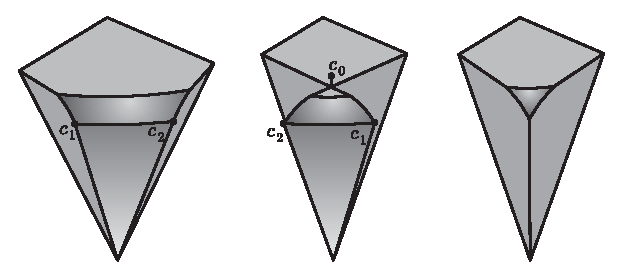
\includegraphics{PS/samfigA54.eps}
  \caption{Different forms of truncated corner cells are shown.  The
  structure
  shown in the middle frame cannot occur.}
  \label{fig:chi-anal-vs-geom}
\end{figure}


We let $c_0$ be the point of height $t_0$ on the intersection of the
planes $\{0,v,v_1\}^\perp$ and $\{0,v,v_2\}^\perp$. We claim that $c_0$ lies
over the truncated spherical region of the tcc, rather than the wedges
of $t_0$-cones or the Rogers simplices along the faces $\{0,v,v_1\}$ and
$\{0,v,v_2\}$.  (This implies that $c_0$ cannot protrude beyond the corner
cell as depicted in the second frame of the figure.) To see the claim,
consider the tcc as a function of $y_4=|v_1-v_2|$. When $y_4$ is
sufficiently large the claim is certainly true.  Contract $y_4$ until
$c_0=c_0(y_4)$ meets the perpendicular bisector of $\{0,v\}$. Then $c_0$
is equidistant from $0,v,v_1$ and $v_2$ so it is the circumcenter of
$\{0,v,v_1,v_2\}$. It has distance $t_0$ from the origin, so the
circumradius is $t_0$. This implies that $y_4\le 2t_0$.

The tcc is defined by the constraints represented in the third frame.
The analytic continuation of the function $\chi_0(S)=\chi_0^\anal(S)$,
defined above, acquires a volume $X$, counted with negative sign, lying
under the spherical triangle $(c_0,c_1,c_2)$. Extending our notation, we
have an analytically defined function $\chi_0^\anal$ and a geometrically
defined function $\chi_0^\geom$,
    $$
    \begin{array}{lll}
    \chi_0^\anal(S) &= \chi_0^\geom(S)-\op{c-vor}_0(X), \text{\ where}\\
    \op{c-vor}_0(X) &= 4(-\doct\op{vol}(X) +\sol(X)/3) = \phi_0\sol(X) <0.
    \end{array}
    $$
So $\chi_0^\anal >\chi_0^\geom$, and we may always use
$\chi_0(S)=\chi_0^\anal(S)$ as an upper bound on the score of a tcc.

For example, with $\lambda=1.6$ and $S = S(2.3,2.3,2.3,2.9,2,2)$, we
have
    $$\chi_0^\anal(S)\approx -0.103981, \quad\chi_0^\geom(S)\approx -0.105102.$$
Or, if $S=S(2,2,2t_0,3.2,2,2t_0)$, then
    $$\chi_0^\anal(S)\approx -0.0718957, \quad
    \chi_0^\geom(S)\approx -0.0726143.$$


\section{Penalties}
    \oldlabel{5.4}
    \label{sec:penalty1}

In Section~\ref{x-4.7}, we determined the bound of
$\maxpi=0.06688$ on penalties. In this section, we give a more
thorough treatment of penalties. Until now a penalty has been
associated with a given standard region, but by taking the worst
case on each subregion, we can move the penalties to the level of
subregions.   Roughly, each subregion should incur the penalties
from the upright quarters that were erased along edges of that
subregion.  Each upright quarter of the original standard region
is attached at an edge between adjacent corners of the standard
cluster. The edges have lengths between $2$ and $2t_0$.  The
deformations shrink the edges to length $2$.  We attach the
penalty from the upright quarter to this edge of this subregion.
In general, we divide the penalty evenly among the upright
quarters along a common diagonal, without trying to determine a
more detailed accounting. For example, the penalty $0.008$ in
Lemma~\ref{lemma:0.008} comes from three upright quarters.  Thus,
we give each of three edges a penalty of $0.008/3$. Or, if there
are only two upright quarters around the $3$-unconfined upright
diagonal, then each of the two upright quarters is assigned the
penalty $0.00222/2$ (see Lemma~\ref{x-3.9.2}).

The penalty $0.04683 = 3\xiG$ in Section~\ref{x-4.7} comes from
three upright quarters around a $3$-crowded upright diagonal. Each
of three edges is assigned a penalty of $\xiG$.  The penalty
$0.03344=3\xiG+\xikG$ comes from a $4$-crowded upright diagonal of
Section~\ref{x-3.8}. It is divided among $4$ edges. These are the
only upright quarters that take a penalty when erased. (The case
of two upright quarters over a flat quarter as in
Lemma~\ref{lemma:unerased}, are treated by a separate argument in
Section~\ref{x-5.7}. Loops will be discussed in
Section~\ref{x-5.11}.)

The penalty can be reduced in various situations involving a
masked flat quarter.  For example, around a $3$-crowded upright
diagonal, if there is a masked flat quarter, two of the upright
quarters are scored by the analytic  function $\svor$, so that the
penalty plus adjustment is only%
\footnote{\calc{73974037}} %A10
\footnote{\calc{764978100}} %A11
 $0.034052=2\xiV+\xiG+0.0114$.
The adjustment $0.0114$ reflects the scoring
rules for masked flat quarters (Lemma~\ref{lemma:0.008}).  This we
divide evenly among the three edges that carried the upright
quarters. If $e$ is an edge of the subregion $R$, let $\pi_0(R,e)$
denote the penalty and score adjustment along edge $e$ of $R$.

In summary, we have the penalties,
    $$\xik,\xiV,\xiG,\ 0.008,$$
combined in various ways in the upright diagonals that are
$3$-unconfined, $3$-crowded, or $4$-crowded.  There are score
adjustments
    $$0.0114\quad \text{ and }\quad 0.0063$$
from Section~\ref{x-3.10} for masked flat quarters.  If the sum of these
contributions is $s$, we set $\pi_0(R,e)=s/n$, for each edge $e$ of $R$
originating from an erased upright quarter of
    $\mathcal{\mathbf S}_n^\pm$.

\section{Penalties and Bounds}
    \oldlabel{5.5}

Recall that the bounds for flat quarters we wish to establish from
Section~\ref{x-4.5} are $Z(3,1)=0.00005$ and $D(3,1)=0.06585$. Flat
quarters arise in two different ways.  Some flat quarters are present
before the deformations begin.  They are scored by the rules of
Section~\ref{x-3.10}. Others are formed by the deformations.  In this
case, they are scored by $\vor_0$. Since the flat quarter is broken away
from the subregion as soon as the diagonal reaches $2\sqrt{2}$, and then
is not deformed further, the diagonal is fixed at $2\sqrt{2}$.  Such
flat quarters can violate our desired inequalities. For example,
    $$
    Z(3,1)<\svor_0(S(2,2,2,2\sqrt{2},2,2)) \approx 0.00898,\quad
        \tau_0(S(2,2,2,2\sqrt{2},2,2))\approx 0.0593.
    $$
On the other hand, as we will see, the adjacent subregion satisfies the
inequality by a comfortable margin.  Therefore, we define a transfer
$\epsilon$ from flat quarters to the adjacent subregion. (In an
exceptional region, the subregion next to a flat quarter along the
diagonal is not a flat quarter.)

For a flat quarter $Q$, set
    $$
    \epsilon_\tau(Q) =
        \begin{cases} 0.0066,&\text{(deformation),}\\
            0,&\text{(otherwise)}.
        \end{cases}
    $$
    %
    $$
    \epsilon_\sigma(Q) =
        \begin{cases}
         0.009,&\text{(deformation),}\\
            0,&\text{(otherwise)}.
        \end{cases}
    $$
The nonzero value occurs when the flat quarter $Q$ is obtained by
deformation from an initial configuration in which $Q$ is not a quarter.
The value is zero when the flat quarter $Q$ appears already in the
undeformed standard cluster. Set
    $$
    \begin{array}{lll}
    \pi_\tau(R) &= \sum_e \pi_0(R,e) +
    \sum_e\pi_0(Q,e)+\sum_Q \epsilon_\tau(Q),\\
    \pi_\sigma(R)&=\sum_e \pi_0(R,e) +
    \sum_e\pi_0(Q,e)+\sum_Q \epsilon_\sigma(Q).
    \end{array}
    $$
The first sum runs over the edges of a subregion $R$.  The second sum
runs over the edges of the flat quarters $Q$ that lie adjacent to $R$
along the diagonal of $Q$.

The edges between corners of the polygon have lengths $2$, $2t_0$, or
$2\sqrt{2}$.  Let $k_0$, $k_1$, and $k_2$ be the number of edges of
these three lengths respectively.  By Lemma~\ref{lemma:7-sides}, we have
$k_0+k_1+k_2\le7$. Let $\tilde\sigma$ denote any of the functions of
Section~\ref{x-3.10}.2(a)--(f). Let $\tilde\tau = \sol\zeta\pt -
\tilde\sigma$.

To prove Theorem~\ref{thm:the-main-theorem}, refining the strategy
proposed in Section~\ref{x-4.5}, we must show that for each flat quarter
$Q$ and each subregion $R$ that is not a flat quarter, we have
    \begin{equation}
    \begin{array}{lll}
    \tilde\tau(Q) &> D(3,1) - \epsilon_\tau(Q),\\
    \tau_0(Q) &> D(3,1)-\epsilon_\tau(Q),\quad\text{if }y_4(Q)=2\sqrt2,\\
    \tau_V(R) &> D(3,2),\quad\text{(type $\SA$)},\\
    \tau_0(R) &> D(k_0+k_1+k_2,k_1+k_2)+\pi_\tau(R),
    %oldtag 5.5.1
    \label{eqn:tau>D(n,k)}
    \end{array}
    \end{equation}
where $D(n,k)$ is the function defined in Section~\ref{x-4.5}. The first
of these inequalities follows.%
% from $\A_{1},\A_{13},\A_{16}$.
\footnote{\calc{193836552}} %A1
\footnote{\calc{148776243}} %A13
\footnote{\calc{163548682}} %A16
In general,
we are given a subregion without explicit information about what the
adjacent subregions are.  Similarly, we have discarded all information
about what upright quarters have been erased.  Because of this, we
assume the worst, and use the largest feasible values of $\pi_\tau$.

\begin{lemma}
We have
    $\pi_\tau(R)\le 0.04683 + (k_0+2k_2-3)0.008/3 +0.0066k_2$.
\end{lemma}

\begin{proof}
The worst penalty $0.04683=3\xiG$ per edge comes from a
$3$-crowded upright diagonal. The number of penalized edges not on
a simplex around a $3$-crowded upright diagonal is at most
$k_0+2k_2-3$. For every three edges, we might have one
$3$-unconfined upright diagonal. The other cases such as
$4$-crowded upright diagonals or situations with a masked flat
quarter are readily seen to give smaller penalties.
\end{proof}

For bounds on the score, the situation is similar.  The only
penalties we need to consider are $0.008$ from
Lemma~\ref{lemma:0.008}. If either of the other configurations of
$3$-crowded or $4$-crowded upright diagonals occur, then the score
of the standard cluster is less than $s_8=-0.228$, by
Sections~\ref{x-3.7} and \ref{x-3.8}. This is the desired bound.
So it is enough to consider subregions that do not have these
upright configurations. Moreover, the penalty $0.008$ does not
occur in connection with masked flats. So we can take
$\pi_\sigma(R)$ to be
    $$(k_0+2k_2)0.008/3 + 0.009 k_2.$$
If $k_0+2k_2<3$, we can strengthen this to
    $\pi_\sigma(R)=0.009 k_2$.
Let $\tilde\sigma$ be any of the functions of Section~\ref{x-3.10}.2
parts (a)--(f). To prove Theorem~\ref{thm:the-main-theorem}, we will
show
    \begin{equation}
    \begin{array}{lll}
    \tilde\sigma(Q)&< Z(3,1)+\epsilon_\sigma(Q),\\
    \svor_0(Q)&< Z(3,1)+\epsilon_\sigma(Q),\quad\text{if }y_4(Q)=2\sqrt2,\\
    \vor_0(R)&< Z(3,2),\quad\text{(type $\SA$)},\\
    \vor_0(R) &< Z(k_0+k_1+k_2,k_1+k_2) - \pi_\sigma(R).
    %oldtag 5.5.2
    \label{eqn:sigma<Z(n,k)}
    \end{array}
    \end{equation}
The first of these inequalities follows.%
\footnote{\calc{193836552}} %A1
\footnote{\calc{148776243}} %A13
\footnote{\calc{163548682}} %A16
% form $\A_1,\A_{13},\A_{16}$.


\section{Penalties} %subsection
\label{sec:4.2} \label{sec:penalty}

Erasing an upright quarter of compression type gives a penalty of
at most $\xiG$ and one of Voronoi type gives at most $\xiV$. We
take the worst possible penalty.  It is at most $n\xiG$ in an
$n$-gon. If there is a masked flat quarter, the penalty is at most
$2\xi_V$ from the two upright quarters along the flat quarter.  We
note in this connection that both edges of a polygon along a flat
quarter lie on upright quarters, or neither does.

If an upright diagonal appears enclosed over a flat quarter, the
flat quarter is part of a loop with context $(n,k)=(4,1)$, for a
penalty at most $2\xi'_\Gamma+\xi_V$.  This is smaller than the
bound on the penalty obtained from a loop with context
$(n,k)=(4,1)$, when the upright diagonal is not enclosed over the
flat quarter:
    $$\xi_\Gamma + 2\xi_V.$$
So we calculate the worst-case penalties under the assumption that
the upright diagonals are not enclosed over flat quarters.

A loop of context $(n,k)=(4,1)$ gives $\xi_\Gamma+2\xi_V$ or
$3\xi_\Gamma$.  A loop of context $(n,k)=(4,2)$ gives
$2\xi_\Gamma$ or $2\xi_V$.

If we erase a $3$-unconfined upright diagonal, there is a penalty
of $0.008$ (or 0 if it masks a flat quarter.) This is dominated by
the penalty $3\xi_\Gamma$ of context $(n,k)=(4,1)$.

Suppose we have an octagonal standard region.  We claim that a
loop does not occur in context $(n,k)=(4,2)$. If there are at most
three vertices that are not corners of the octagon, then there are
at most 12 quasi-regular tetrahedra, and the score is at most
$$s_8 + 12\,\pt<8\,\pt.$$
Assume there are more than three vertices that are not corners
over the octagon. We squander
$$t_8+ \dloop(4,2)+4\tlp(5,0) > \squander.$$
As a consequence, context $(n,k)=(4,2)$ does not occur.

So there are at most $2$ upright diagonals and at most $6$
quarters, and the penalty is at most $6\xi_\Gamma$. Let $f$ be the
number of flat quarters This leads to
    $$
    \piF = \begin{cases} 6\xiG, & f=0,1,\\
                   4\xiG+2\xiV, & f=2,\\
                    2\xiG+4\xiV, & f=3,\\
                    0, & f=4.
            \end{cases}
    $$
The 0 is justified by a parity argument.  Each upright quarter
occurs in a pair at each masked flat quarter.  But there is an odd
number of quarters along the upright diagonal, so no penalty at
all can occur.

Suppose we have a heptagonal standard region.  Three loops are a
geometric impossibility. Assume there are at most two upright
diagonals.
 If there is no context $(n,k)=(4,2)$,
 then we have the following bounds on the penalty
    $$
    \piF = \begin{cases} 6\xiG, & f=0,\\
                 4\xiG+2\xiV, & f=1,\\
                3\xiG, & f=2,\\
                \xiG+2\xiV, & f=3.
            \end{cases}
    $$
If an upright diagonal has context $(n,k)=(4,2)$, then
    $$
    \piF = \begin{cases} 5\xiG, & f=0,1,\\
                3\xiG + 2\xiV, & f=2,\\
                \xiG + 4 \xiV, &f = 3.\\
            \end{cases}
    $$
This gives the bounds used in the diagrams of cases.



\section{Constants}
    \oldlabel{5.6}

Theorem~\ref{thm:the-main-theorem} now results from the calculation of a
host of constants. Perhaps there are simpler ways to do it, but it was a
routine matter to run through the long list of constants by computer.
What must be checked is that the Inequalities~\ref{eqn:tau>D(n,k)}
and~\ref{eqn:sigma<Z(n,k)} of Section~\ref{x-5.5} hold for all possible
convex subregions. Call these inequalities the {\it D} and {\it Z}
inequalities.  This section describes in detail the constants to check.

We begin with a subregion given as a convex $n$-gon, with at least $4$
sides.   The heights of the corners and the lengths of edges between
adjacent edges have been reduced by deformation to a finite number of
possibilities (lengths $2$, $2t_0$, or lengths $2$, $2t_0$, $2\sqrt{2}$,
respectively). By Lemma~\ref{lemma:7-sides}, we may take $n=4,5,6,7$.
Not all possible assignments of lengths correspond to a geometrically
viable configuration. One constraint that eliminates many possibilities,
especially heptagons, is that of Section~\ref{x-5.1}: the perimeter of
the convex polygon is at most a great circle.  Eliminate all
length-combinations that do not satisfy this condition.  When there is a
special simplex it can be broken
from the subregion and scored\footnote{\calc{148776243}} %A13
separately unless the two heights along the diagonal are $2$.
We assume in all that follows that all specials that can be
broken off have been. There is a second condition related to special
simplices.  We have
    $\Delta(2t_0^2,2^2,2^2,x^2,2^2,2^2)<0$, if $x> 3.114467$.
This means that if the cluster edges along the polygon are
$(y_1,y_2,y_3,y_5,y_6)= (2t_0,2,2,2,2)$, the simplex must be special
($y_4\in[2\sqrt{2},3.2]$).

The easiest cases to check are those with no special simplices over the
polygon.  In other words, these are subregions for which the distances
between nonadjacent corners are at least $3.2$.  In this case we
approximate the score (and what is squandered) by tccs at the corners.
We use monotonicity to bring the fourth edge to length $3.2$. We
calculate the tcc constant bounding the score, checking that it is less
than the constant
    $ Z(k_0+k_1+k_2,k_1+k_2) - \pi_\sigma$,
from the Z inequalities. The D inequalities  are verified in the same
way.

When $n=5,6,7,$ and there is one special simplex, the situation is not
much more difficult.  By our deformations,  we decrease the lengths of
edges $2,3,5,6$ of the special to 2. We remove the special by cutting
along its fourth edge $e$ (the diagonal).  We score the special with
weak bounds.\footnote{\calc{148776243}} %A13  found in $\A_{13}$.
Along the edge $e$, we then apply
deformations to the $(n-1)$-gon that remains. If this deformation brings
$e$ to length $2\sqrt{2}$, then the $(n-1)$-gon may be scored with tccs
as in the previous paragraph.  But there are other possibilities. Before
$e$ drops to $2\sqrt{2}$, a new distinguished edge of length $3.2$ may
form between two corners (one of the corners will be a chosen endpoint
of $e$).  The subregion breaks in two. By deformations, we eventually
arrive at $e=2\sqrt2$ and a subregion with diagonals of length at least
$3.2$.  (There is one case that may fail to be deformable to
$e=2\sqrt2$, a pentagonal cases discussed further in
Section~\ref{x-5.9}.) The process terminates because the number of sides
to the polygon drops at every step. A simple recursive computer
procedure runs through all possible ways the subregion might break into
pieces and checks that the tcc-bound gives the $D$ and $Z$ inequalities.
The same argument works if there is a special simplex that overlaps each
of the other special simplices in the subcluster.

When $n=6,7$ and there are two nonoverlapping special simplices, a
similar argument can be applied. Remove both specials by cutting along
the diagonals. Then deform both diagonals to length $2\sqrt{2}$, taking
into account the possible ways that the subregion can break into pieces
in the process.  In every case the $D$ and $Z$ inequalities are
satisfied.

There are a number of situations that arise that escape this generic
argument and were analyzed individually. These include the cases
involving more than two special simplices over a given subregion, two
special simplices over a pentagon, or a special simplex over a
quadrilateral.  Also, the deformation lemmas are insufficient to bring
all of the edges between adjacent corners to one of the three standard
lengths $2,2t_0,2\sqrt{2}$ for certain triangular and quadrilateral
regions.  These are treated individually.

The next few sections describe the cases treated individually. The cases
not mentioned in the sections that follow fall within the generic
procedure just described.

\section{Triangles}
    \oldlabel{5.7}

With triangular subregions, there is no need to use any of the
deformation arguments because the dimension is already sufficiently
small to apply interval arithmetic directly to obtain our bounds.
There is no need for the tcc-bound approximations.

Flat quarters and simplices of type $\SA$ are treated by a computer
calculation.\footnote{\calc{163548682}} %A16
Other simplices are scored by the truncated function
$\svor_0$. We break the edges between corners into the cases
    %((
    $[2,2t_0)$, $[2t_0,2\sqrt{2})$, $[2\sqrt{2},3.2]$.
    %]]
Let $k_0$, $k_1$, and $k_2$, with $k_0+k_1+k_2=3$, be the number
of edges  in the respective intervals.

If $k_2=0$, we can improve the penalties,
    $$\pi_\tau = \pi_\sigma=0.$$
To see this, first we observe that there can be no $3$-crowded or
$4$-crowded upright diagonals. By placing $\ge3$ quarters around
an upright diagonal, if the subregion is triangular, the upright
diagonal becomes surrounded by anchored simplices, a case deferred
until Section~\ref{x-5.11}.

If $k_0=k_1=k_2=1$, we can take $\pi'_\tau=
\xiG+2\xiV+0.0114=0.034052$. A few cases are needed to justify
this constant. If there are no $3$-crowded upright diagonals,
$\pi'_\tau$ is at most
    $$
    \begin{array}{lll}
    &[\xiG + 2 \xiV +\xikG ]3/4 < 0.0254,\\
    \hbox{or\quad }&[\xiG+2\xiV+\xikG]2/4 + 0.008/3 < 0.0254
    \end{array}
    $$
If there are at most two edges in the subregion coming from an
$3$-crowded upright diagonal,
    $$(\xiG+2\xiV+0.0114)2/3 + 0.008/3 < 0.0254.$$
If three edges come from the simplices of a $3$-crowded upright
diagonal, we get $0.034052$. To get somewhat sharper bounds, we
consider how the edge $k_2$ was formed.  If it is obtained by
deformation from an edge in the standard region of length
$\ge3.2$, then it becomes a distinguished edge when the length
drops to $3.2$.  If the edge in the standard region already has
length $\le3.2$, then it is distinguished before the deformation
process begins, so that the subregion can be treated in isolation
from the other subregions. We conclude that when
$\pi'_\tau=0.034052$ we can take $y_4\ge2.6$ or $y_5=3.2$
(Remark~\ref{remark:2.6}).

The $D$ and $Z$ inequalities now follow.%
\footnote{\calc{852270725}} %A17
\footnote{\calc{819209129}} %A18
% from $\A_{17}$ and $\A_{18}$.

\section{Quadrilaterals}
    \oldlabel{5.8}

We introduce some notation for the heights and edge lengths of a convex
polygon.  The heights will generally be $2$ or $2t_0$, the edge lengths
between consecutive corners will generally be $2$, $2t_0$, or
$2\sqrt{2}$.  We represent the edge lengths by a vector
    $$(a_1,b_1,a_2,b_2,\ldots,a_n,b_n),$$
if the corners of an $n$-gon, ordered cyclically have heights $a_i$ and
if the edge length between corner $i$ and $i+1$ is $b_i$.  We say two
vectors are equivalent if they are related by a different cyclic
ordering on the corners of the polygon, that is, by the action of the
dihedral group.

The vector of a polygon with a special simplex is equivalent to one of
the form
    $$(2,2,a_2,2,2,\ldots).$$  If $a_2=2t_0$, then what we have is
necessarily special (Section~\ref{x-5.6}). However, if $a_2=2$, it is
possible for the edge opposite $a_2$ to have length greater than $3.2$.


Turning to quadrilateral regions, we use tcc scoring if both diagonals
are greater than $3.2$.   Suppose that both diagonals are between
$[2\sqrt{2},3.2]$, creating a pair of overlapping special simplices. The
deformation lemma requires a diagonal longer than $3.2$, so although we
can bring the quadrilateral to the form
    $$(a_1,2,2,2,2,2,a_4,b_4),$$
the edges $a_1,a_4,b_4$ and the diagonal vary%
\footnote{\calc{148776243}} %A13  (see $\A_{13}$).
continuously.
We have bounds\footnote{\calc{128523606}} %A19
 on the score
    $$
    \begin{array}{lll}
    \tau_0 &> 0.235, \quad \vor_0 < -0.075,
                \hbox{ if } b_4\in[2t_0,2\sqrt{2}],\\
    \tau_0 &> 0.3109, \quad \vor_0 < -0.137,
                \hbox{ if } b_4\in[2\sqrt{2},3.2],\\
    \end{array}
    $$
We have $D(4,1)=0.2052$, $Z(4,1)=-0.05705$. When
$b_4\in[2t_0,2\sqrt{2}]$, we can take $\pi_\tau=\pi_\sigma=0$. (We are
excluding loops here.) When $b_4\in[2\sqrt{2},3.2]$, we can take
    $$
    \begin{array}{lll}
    \pi_\tau &= \maxpi+ 0.0066, \\
    \pi_\sigma &= 0.008 (5/3)+ 0.009. \\
    \end{array}
    $$
It follows that the $D$ and $Z$ Inequalities are satisfied.

Suppose that one diagonal has length $[2\sqrt{2},3.2]$ and the other has
length at least $3.2$.  The quadrilateral is represented by the vector
    $$(2,2,a_2,2,2,b_3,a_4,b_4).$$
The hypotheses of the deformation lemma hold, so that $a_i\in\{2,2t_0\}$
and $b_j\in\{2,2t_0,2\sqrt2\}$. To avoid quad clusters, we assume
$b_4\ge\max(b_3,2t_0)$. These are one-dimensional with a diagonal of
length $[2\sqrt{2},3.2]$ as parameter.
 The required verifications\footnote{\calc{874876755}} %A20
have been made by interval arithmetic.
%appear in $\A_{20}$.


\section{Pentagons}
    \oldlabel{5.9}

Some extra comments are needed when there is a special simplex. The
general argument outlined above removes the special, leaving a
quadrilateral.  The quadrilateral is deformed, bringing the edge that
was the diagonal of the special to $2\sqrt{2}$. This section discusses
how this argument might break down.

Suppose first that there is a special and that both diagonals on the
resulting quadrilateral are at least $3.2$.  We can deform using either
diagonal, keeping both diagonals at least $3.2$. The argument breaks
down if both diagonals drop to $3.2$ before the edge of the special
reaches $2\sqrt{2}$ and both diagonals of the quadrilateral lie on
specials. When this happens, the quadrilateral has the form
    $$(2,2,2,2,2,2,2,b_4),$$
where $b_4$ is the edge originally on the special simplex.  If both
diagonals are $3.2$, this is rigid, with $b_4= 3.12$. We find its score
to be
    $$
    \begin{array}{lll}
    &\svor_0(S(2,2,2,b_4,3.2,2))+\svor_0(S(2,2,2,3.2,2,2))+0.0461<-0.205,\\
    &\tau_0(S(2,2,2,b_4,3.2,2))+\tau_0(S(2,2,2,3.2,2,2))2> 0.4645.\\
    \end{array}
    $$
So the $D$ and $Z$ Inequalities hold easily.

If there is a special and there is a diagonal on resulting quadrilateral
$\le3.2$, we have two nonoverlapping specials.  It has the form
    $$(2,2,a_2,2,2,2,a_4,2,2,b_5).$$
The edges $a_2$ and $a_4$ lie on the special.  If $b_5>2$, cut
away one of the special simplices.  What is left can be reduced to
a triangle, or a quadrilateral case and then treated%
\footnote{\calc{874876755}} %A20
by computer. % in $\A_{20}$.
Assume
$b_5=2$.  We have a pentagonal standard region. We may assume that
there is no $3$-crowded or $4$-crowded upright diagonal, for
otherwise Theorem~\ref{thm:the-main-theorem} follows trivially
from the bounds in Section~\ref{x-2}. A pentagon can then have at
most a $3$-unconfined upright diagonal for a penalty of $0.008$.

If $a_2=2t_0$ or $a_4=2t_0$, we again remove a special simplex and
produce triangles, quadrilaterals, or the special cases treated
by computer.%
\footnote{\calc{874876755}} %A20
We may impose the condition $a_2=a_4=b_5=2$. We score this full pentagonal
arrangement by computer,\footnote{\calc{692155251}} %A21 $\A_{21}$,
using the edge lengths of the two diagonals of
the specials as variables. The inequalities follow.

\section{Hexagons and heptagons}
    \oldlabel{5.10}

We turn to hexagons. There may be three specials whose diagonals do not
cross.  Such a subcluster is represented by the vector
    $$(2,2,a_2,2,2,2,a_4,2,2,2,a_6,2).$$
The heights $a_{2i}$ are $2$ or $2t_0$.  Draw the diagonals between
corners $1$, $3$, and $5$.  This is a three-dimensional configuration,
determined by the lengths of the three diagonals, which is treated
by computer.\footnote{\calc{692155251}} %A21
%The required bound follows from $\A_{21}$.

There is one case with a special simplex that
did not satisfy the generic computer-checked inequalities for
what is to be squandered.  Its vector is
    $$(a_1,2,2,2,2,2,2,b_4,2,2,2,2),$$
with $a_1=b_4=2t_0$. A vertex of the special simplex has height
$a_1=2t_0$ and all other corners have height $2$.  The subregion
is a hexagon with one edge longer than $2$.  We have $D(6,1)=
0.48414$. This is certainly obtained if the subregion contains a
$3$-crowded upright diagonal, squandering $0.5606$. But if this
configuration does not appear, we can decrease $\pi_\tau$ to
    $0.03344 + (2/3) 0.008$,
a constant coming from $4$-crowded upright diagonals in
Section~\ref{x-4.7}. With this smaller penalty the inequality is
satisfied.

Now turn to heptagons.The bound $2\pi$  on the perimeter of the polygon,
eliminates all but one equivalence class of vectors associated with a
polygon that has two or more potentially specials simplices. The vector
is
    $$(2,2,a_2,2,2,2,a_4,2,2,2,a_6,2,a_7,2),$$
$a_2=a_4=a_6=a_7=2t_0$. In other words, the edges between adjacent
corners are $2$ and four heights are $2t_0$. There are two specials.
This case is treated by the procedure outlined for subregions with two
specials whose diagonals do not cross.

\section{Loops}
    \oldlabel{5.11}
    \label{sec:loops}

We now return to a collection of anchored simplices that surround
the upright diagonal.  This is the last case needed to complete
the proof of Theorem~\ref{x-4.3}. There are four or five anchored
simplices around the upright diagonal.
There are linear inequalities%
\footnote{\calc{815492935}} %A2
\footnote{\calc{729988292}} %A3
\footnote{\calc{531888597}} %A4
\footnote{\calc{628964355}} %A5
\footnote{\calc{934150983}} %A6
\footnote{\calc{187932932}} %A7
%$\A_2$--$\A_7$ give a list
%of linear inequalities
satisfied by the anchored simplices, broken
up according to type: upright, type $\SC$, opposite edge $>3.2$,
etc. The anchored simplices are related by the constraint that the
sum of the dihedral angles around the upright diagonal is $2\pi$.
We run a linear program in each case based on these linear
inequalities, subject to this constraint to obtain bounds on the
score and what is squandered by the anchored simplices.

When the edge opposite the diagonal of an anchored simplex has length
$\in[2\sqrt{2},3.2]$ and the simplex adjacent to the anchored simplex
across that edge is a special simplex, we use inequalities%
\footnote{\calc{485049042}} %A22
\footnote{\calc{209361863}} %A23
% $\A_{22}$ and $\A_{23}$
that run parallel to the similar system\footnote{\calc{531888597}} %A4
\footnote{\calc{628964355}} %A5
%$\A_4$ and $\A_5$.
It is not
necessary to run separate linear programs for these.  It is enough to
observe that the constants for what is squandered improve on those from
the similar system\footnote{\calc{531888597}} %A4
%$\A_4$ by at least $0.06445$
and that the constants for the score in one system%
\footnote{\calc{485049042}} %A22
differ with those of the other%
\footnote{\calc{531888597}} %A4
by no more than $0.009$.

When the dihedral angle of an anchored simplex is greater than $2.46$,
the simplex is dropped, and the remaining anchored simplices are subject
to the constraint that their dihedral angles sum to at most $2\pi-2.46$.
There can not be an anchored simplex with dihedral angle greater than
$2.46$ when there are five anchors: $2.46+4 (0.956)>2\pi$. There cannot%
\footnote{\calc{83777706}} %A8
be two anchored simplices with dihedral angle greater than $2.46$:
$2(2.46+0.956)>2\pi$.

The following table summarizes the linear programming results.

$$
\begin{matrix}
(n,k)   &   \DLP(n,k) & D(n,k)      &\ZLP(n,k)  &Z(n,k)\\
(4,0)   &   0.1362  &   0.1317  &   0   &   0\\
(4,1)   &   0.208   &   0.20528 &-0.0536&   -0.05709\\
(4,2)   &   0.3992  &   0.27886 &-0.2   &   -0.11418\\
(4,3)   &  0.6467   &   0.35244 &-0.424 &   -0.17127\\
(5,0)   &   0.3665  &   0.27113 &-0.157 &   -0.05704\\
(5,1)   &  0.5941   &   0.34471 &-0.376 &   -0.11413\\
(5,\ge2)&  0.9706   &  \squander    &*          &   *
\end{matrix}
$$

The bound for $D(4,0)$ comes from Lemma~\ref{lemma:0.1317}. A few
more comments are needed for $Z(4,1)$.  Let $S=S(y_1,\ldots,y_6)$
be the anchored simplex that is not a quarter.  If $y_4\ge2\sqrt2$
or $\dih(S)\ge 2.2$, the linear programming bound is $<Z(4,1)$.
With this, if $y_1\le 2.75$, we have\footnote{\calc{855294746}} %A12
    $\sigma(S) < Z(4,1)$.
But if $y_1\ge2.75$, the $3$ upright quarters along the
upright diagonal satisfy
    $$\nu< -0.3429+0.24573\dih.$$
With this stronger inequality, the linear programming bound becomes
$<Z(4,1)$. This completes the proof of
Theorem~\ref{thm:the-main-theorem}.

\begin{lemma}\label{lemma:loop}
Consider an upright diagonal that is a loop.  Let $R$ be the
standard region that contains the upright diagonal and its
surround simplices.   Then the following contexts $(m,k)$ are the
only ones possible.  Moreover, the constants that appear in the
columns marked $\sigma$ and $\tau$ are upper and lower bounds
respectively for $\tau_R(D)$ when $R$ contains one loop of that
context.
    $$
    \begin{array}{llll}
        n=n(R)&(m,k) &\sigma &\tau \\
        &&&\\
        4& & &\\
        &(4,0) &-0.0536 & 0.1362 \\
        5 & & &\\
        &(4,1) &s_5 &0.27385\\
        &(5,0) &-0.157   &0.3665\\
        6 & & &\\
        &(4,1) &s_6 &0.41328\\
        &(4,2) &-0.1999  &0.5309\\
        &(5,1) &-0.37595 &0.65995\\
        7 & & &\\
        &(4,1) &s_7 &0.55271\\
        &(4,2) &-0.25694 &0.67033\\
        8 & & &\\
        &(4,1) &s_8 &0.60722\\
        &(4,2) &-0.31398 &0.72484
    \end{array}
    $$
\end{lemma}

\begin{proof} In context $(m,k)$, and if $n=n(R)$, we have
    $$
    \sigma_R(D) < s_{n} + \ZLP(m,k)-Z(m,k)\quad
    \tau_R(D)> t_{n}+\DLP(m,k)-D(m,k).
    $$
The result follows.
\end{proof}

In the context $(n,k)=(4,3)$, the standard region $R$ must have at
least seven sides $n(R)\ge7$.   Then
    $$
    \begin{array}{lll}
    \tau(D)&\ge t_7+\dloop(4,3)\\
            &>\squander.
    \end{array}
    $$
Thus, we may assume that this context does not occur.

If the context $(5,1)$ appears in an octagon, we have
    $$\tau(D) >\dloop(5,1)+t_8>\squander.$$
If this appears in a heptagon, we have
$$\tau(D) >\dloop(5,1) + t_7+ 0.55\,\pt > \squander,$$
because there must be a vertex that is not a corner of the
heptagon. It cannot appear on a pentagon.





\chapter{Further Bounds in Exceptional Regions}
    \oldlabel{5.12}
    \label{sec:fb}

\section{Small dihedral angles}\label{sec:small-dih}

Recall that Section~\ref{sec:the-main-theorem} defines an integer $n(R)$
that is equal to the number of sides if the region is a polygon.  Recall
that if the dihedral angle along an edge of a standard cluster is at
most $1.32$, then there is a flat quarter along that edge
(Lemma~\ref{x-3.11.4}).

\begin{lemma}
    \oldlabel{5.12.1}
Let $R$ be an exceptional cluster with a dihedral angle
$\le1.32$ at a vertex $v$. Then $R$ squanders $>t_n+1.47\,\pt$, where
$n=n(R)$.
\end{lemma}

\begin{proof}
In most cases we establish the stronger bound $t_n+1.5\,\pt$. In the
proof of Theorem~\ref{thm:the-main-theorem}, we erase all upright
diagonals, except those completely surrounded by anchored simplices. The
contribution to $t_n$ from the flat quarter $Q$ at $v$ in that proof is
$D(3,1)$ (Sections~\ref{x-4.5} and Inequalities~\ref{eqn:tau>D(n,k)}).
Note that $\epsilon_\tau(Q)=0$ here because there are no deformations.
If we replace $D(3,1)$ with $3.07\,\pt$ from Lemma~\ref{x-3.11.4}, then
we obtain the bound. Now suppose the upright diagonal is completely
surrounded by anchored simplices. Analyzing the constants of
Section~\ref{x-5.11}, we see that $\DLP(n,k)-D(n,k)>1.5\,\pt$ except
when $(n,k)=(4,1)$.

Here we have four anchored simplices around an upright diagonal. Three
of them are quarters.  We erase and take a penalty. Two possibilities
arise.  If the upright diagonal is enclosed over the flat quarter, its
height is $\ge2.6$ by geometric considerations and the top face of the
flat quarter has circumradius at least $\sqrt2$.  The penalty is
$2\xiG'+\xiV$, so the bound holds by the last statement of
Lemma~\ref{x-3.11.4}.

If, on the other hand, the upright diagonal is not enclosed over the
flat diagonal, the penalty is $\xiG+2\xiV$.  In this case, we obtain the
weaker bound $1.47\,\pt+t_n$:
    $$3.07\,\pt > D(3,1) + 1.47\,\pt +\xiG+2\xiV.$$
\end{proof}

\begin{remark} \label{remark:1.47}
If there are $r$ nonadjacent vertices with dihedral angles
$\le1.32$, we find that $R$ squanders $t_n+r(1.47)\,\pt$.
\end{remark}

In fact, in the proof of the lemma, each $D(3,1)$ is replaced with
$3.07\,\pt$ from Lemma~\ref{x-3.11.4}.  The only questionable case
occurs when two or more of the vertices are anchors of the same upright
diagonal (a loop). Referring to Section~\ref{x-5.11}, we have the
following observations about various contexts.

\begin{itemize}
    \item $(4,1)$ can mask only one flat quarter and it is treated in the
lemma.
    \item $(4,2)$ can mask only one flat quarter and
    $\DLP(4,2)-D(4,2)>1.47\,\pt$.
    \item $(5,0)$ can mask two flat quarters.  Erase the five upright quarters,
        and take a penalty $4\xiV+\xiG$.  We get
    $$D(3,2)+2(3.07)\,\pt > t_5+4\xiV+\xiG+2(1.47)\,\pt.$$
    \item $(5,1)$ can mask two flat quarters, and $\DLP(5,1)-D(5,1)>2(1.47)\,\pt$.
\end{itemize}




\section{A particular $4$-circuit}

This subsection bounds the score of a particular four-circuit on a
contravening plane graph.  The interior of the circuit consists of
two faces: a triangle and a pentagon.  The circuit and its
enclosed vertex are show in Figure \ref{fig:no4circuit} with
vertices marked $p_1,\ldots,p_5$.  The vertex $p_1$ is the
enclosed vertex, the triangle is $(p_1,p_2,p_5)$ and the pentagon
is $(p_1,\ldots,p_5)$.

\begin{figure}[htb]
  \centering
  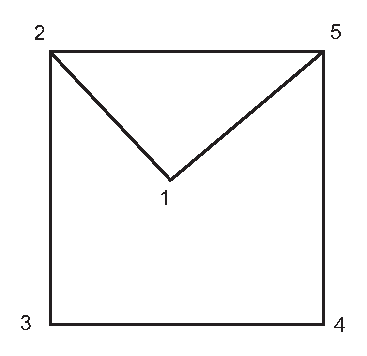
\includegraphics{PS/no4circuit.eps}
  \caption{A $4$-circuit}
  \label{fig:no4circuit}
\end{figure}

Suppose that $D$ is a decomposition star whose associate graph
contains such triangular and pentagonal standard regions.  Recall
that $D$ determines a set $U(D)$ of vertices in Euclidean $3$-space
of distance at most $2t_0$ from the origin, and that each vertex
$p_i$ can be realized geometrically as a point on the unit sphere at
the origin, obtained as the radial projection of some $v_i\in U(D)$.

\begin{lemma}  One of the edges $\{v_1,v_3\}$, $\{v_1,v_4\}$ has
length less than $2\sqrt{2}$.  Both of the them have lengths less
than $3.02$. Also, $|v_1|\ge2.3$.
\end{lemma}

\begin{proof}
This is a standard exercise in geometric considerations as
introduced in Section~\ref{sec:decomposition}.  (The reader should
review that section for the framework of the following argument.)
We deform the figure using pivots to a configuration
$v_2,\ldots,v_5$ at height $2$, and $|v_i-v_j|=2t_0 $,
$(i,j)=(2,3),(3,4),(4,5),(5,2)$. We scale $v_1$ until $|v_1|=2t_0
$. We can also take the distance from $v_1$ to $v_5$ and to $v_2$
to be $2$. If we have $|v_1-v_3|\ge 2\sqrt{2}$, then we stretch
the edge $|v_1-v_4|$ until $|v_1-v_3|=2\sqrt{2}$. The resulting
configuration is rigid.  Pick coordinates to find that
$|v_1-v_4|<2\sqrt{2}$. If we have $|v_1-v_3|\ge 2t_0 $, follow a
similar procedure to reduce to the rigid configuration
$|v_1-v_3|=2t_0$, to find that $|v_1-v_4|<3.02$. The estimate
$|v_1|\ge2.3$ is similar.
\end{proof}

There are restrictive bounds on the dihedral angles of the
simplices $\{0,v_1,v_i,v_j\}$ along the edge $\{0,v_1\}$. The
quasi-regular tetrahedron has a dihedral angle of at most%
\footnote{\calc{984463800}} $1.875$.  The dihedral angles of the
simplices $\{0,v_1,v_2,v_3\}$, $\{0,v_1,v_5,v_4\}$
adjacent to it are at most%
\footnote{\calc{821707685}}  $1.63$. The dihedral angle of the
remaining simplex $\{0,v_1,v_3,v_4\}$ is at most%
\footnote{\calc{115383627}} $1.51$.   This leads to lower bounds
as well. The quasi-regular tetrahedron has a dihedral angle that
is at least $2\pi - 2(1.63)-1.51 > 1.51$.  The dihedral angles
adjacent to the quasi-regular tetrahedron is at least $2\pi-
1.63-1.51-1.875> 1.26$. The remaining dihedral angle is at least
$2\pi-1.875-2(1.63) > 1.14$.

A decomposition star $D$ determines a set of vertices $U(D)$ that
are of distance at most $2t_0$ from the center of $D$.  Three
consecutive vertices $p_1$, $p_2$, and $p_3$ of a standard region
are determined as the projections to the unit sphere of three
corners $v_1$, $v_2$, and $v_3$, respectively in $U(D)$. By
Lemma~\ref{lemma:1.32}, if the interior angle of the standard
region is less than $1.32$, then $|v_1-v_3|\le\sqrt{8}$.

\begin{lemma} \label{lemma:11.16}
These two standard regions $F=\{R_1,R_2\}$ give
    $\tau_F(D) \ge 11.16\,\pt$.
\end{lemma}

\begin{proof}
Let $\dih$ denote the dihedral angle of a simplex along a given
edge. Let $S_{ij}$ be the simplex $\{0,v_1,v_i,v_j\}$, for
$(i,j)=(2,3),(3,4), (4,5),(2,5)$. We have $\sum_{(4)}\dih(S_{ij})
= 2\pi$. Suppose one of the edges $\{v_1,v_3\}$ or $\{v_1,v_4\}$ has
length $\ge2\sqrt2$. Say $\{v_1,v_3\}$.

We have\footnote{\calc{572068135}, \calc{723700608},
\calc{560470084}, and \calc{535502975}}
    $$
    \begin{array}{lll}
    \tau(S_{25}) &- 0.2529\dih(S_{25}) > -0.3442,\\
    \tau_0(S_{23}) &- 0.2529\dih(S_{23}) > -0.1787,\\
    \hat\tau(S_{45}) &- 0.2529\dih(S_{45}) > -0.2137,\\
    \tau_0(S_{34}) &- 0.2529\dih(S_{34}) > -0.1371.\\
    \end{array}
    $$
We have a penalty $\xiG$ for erasing, so that
    $$
    \begin{array}{lll}
        \tau(D) &\ge \sum_{(4)}\tau_x(S_{ij}) - 5\xiG\\
                &>2\pi(0.2529)-0.3442\\
                &\qquad -0.1787-0.2137-0.1371-5\xiG\\
                &>11.16\,\pt,
    \end{array}
    $$
where $\tau_x=\tau,\hat\tau,\tau_0$ as appropriate.

Now suppose $\{v_1,v_3\}$ and $\{v_1,v_4\}$ have length $\le2\sqrt2$.
If there is an upright diagonal that is not enclosed over either
flat quarter, the penalty is at most $3\xiG+2\xiV$. Otherwise, the
penalty is smaller: $4\xiG'+\xiV$. We have
    $$
    \begin{array}{lll}
    \tau(D)
    &\ge \sum_{(4)}\tau(S_{ij})-(3\xiG+2\xiV)\\
    &>2\pi(0.2529)-0.3442\\
    &\qquad -2(0.2137)-0.1371 -(3\xiG+2\xiV)\\
    &>11.16\,\pt.\\
    \end{array}
    $$
\end{proof}

\section{A particular $5$-circuit}

\begin{lemma}\label{lemma:6079}  Assume that $R$ is a pentagonal standard region
    with an enclosed vertex $v$ of height at most $2t_0$.
    %(See Figure~\ref{fig:pent-tri1}.)
    Assume further that
    \begin{itemize}
        \item $|v_i|\le 2.168$ for each of the five corners.
        \item Each interior angle of the pentagon is at most
        $2.89$.
        \item If $v_1$, $v_2$, $v_3$ are consecutive corners over
        the pentagonal region, then $$|v_1-v_2|+|v_2-v_3|<4.804.$$
        \item $\sum_5 |v_i-v_{i+1}|\le 11.407.$
    \end{itemize}
    Then $\sigma_R(D)< -0.2345$ or $\tau_R(D) > 0.6079.$
\end{lemma}

%\begin{figure}[htb]
%  \centering
%  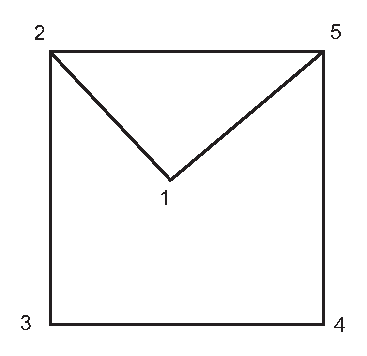
\includegraphics{PS/no4circuit.eps}
%  \caption{A pentagon and triangle}
%  \label{fig:pent-tri1}
%\end{figure}


\begin{proof}
Since $-0.4339$ is less than this the lower bound, a $3$-crowded
upright diagonal does not occur. Similarly, since $-0.25$ is less
than the lower bound, a $4$-crowded upright diagonal does not
occur (Lemma~\ref{lemma:4-crowded} and Lemma~\ref{x-3.8}).

Suppose that there is a loop in context $(n,k)=(4,2)$. Again by
Lemma~\ref{lemma:loop} (with $n(R)=7$),
$$\sigma_R(D)  < -0.2345.$$
%The constants come from
%Table~\ref{x-5.11} and  Theorem~\ref{thm:the-main-theorem}.

%If we branch and bound on the triangular faces, this LP-derived
%inequality can be improved to
%    $$\tau[F] < 0.6079.$$

%If there is a loop other than $(4,2)$ and $(4,1)$, the linear
%program becomes infeasible:
%    $$\tau[F] < 0.644 < t_7 + \dloop(n,k) < \tau[F].$$
We conclude that all loops have context $(n,k)=(4,1)$.


{\bf Case 1.}  {\it The vertex $v=v_{12}$ has distance at least
$2t_0$ from the five corners of $U(D)$ over the pentagon.}

%The interval calculations relevant in Case 1 appear in
%~\ref{A.3.8}.

The penalty to switch the pentagon to a pure $\vor_0$ score is at
most $5\xiG$ (see Section~\ref{sec:prep-cluster}).  There cannot
be two flat quarters because then
$$|v_{12}|>\CalE(S(2,2,2,2t_0,2\sqrt2,2\sqrt2),2t_0,2t_0,2t_0)>2t_0.$$

{\bf (Case 1-a)} Suppose there is one flat quarter,
$|v_1-v_4|\le2\sqrt2$. There is a lower bound of 1.2 on the
dihedral angles of the simplices $\{0,v_{12},v_i,v_{i+1}\}$.  This
is obtained as follows.  The proof relies on the convexity of the
quadrilateral region.  We leave it to the reader to verify that
the following pivots can be made to preserve convexity.  Disregard
all vertices except $v_1,v_2,v_3,v_4,v_{12}$.  We give the
argument that $\dih(0,v_{12},v_1,v_4)>1.2$.  The others are
similar. Disregard the length $|v_1-v_4|$.  We show that
    $$
    \begin{array}{lll}
        sd &:=\dih(0,v_{12},v_1,v_2)+\dih(0,v_{12},v_2,v_3)\\
           &+\dih(0,v_{12},v_3,v_4) < 2\pi-1.2.
    \end{array}
    $$
Lift $v_{12}$ so $|v_{12}|=2t_0$. Maximize $sd$ by taking
$|v_1-v_2|=|v_2-v_3|=|v_3-v_4|=2t_0$.  Fixing $v_3$ and $v_4$,
pivot $v_1$ around $\{0,v_{12}\}$ toward $v_4$, dragging $v_2$
toward $v_{12}$ until $|v_2-v_{12}|=2t_0$.  Similarly, we obtain
$|v_3-v_{12}|=2t_0$. We now have $sd\le 3(1.63)< 2\pi-1.2$, by a
calculation.\footnote{\calc{821707685}}

Return to the original figure and move $v_{12}$ without increasing
$|v_{12}|$ until each simplex $\{0,v_{12},v_i,v_{i+1}\}$ has an edge
$(v_{12},v_j)$ of length $2t_0$. Interval
calculations\footnote{\calc{467530297} and \calc{135427691}} show
that the four simplices around $v_{12}$ squander
    $$2\pi(0.2529)-3(0.1376)-0.12 > \squander + 5\xiG.$$

{\bf (Case 1-b)} Assume there are no flat quarters. By hypothesis,
the perimeter satisfies $$\sum|v_i-v_{i+1}|\le 11.407.$$ We have
$\arc(2,2,x)'' = 2x/(16-x^2)^{3/2} >0$. The arclength of the
perimeter is therefore at most
$$2\arc(2,2,2t_0) + 2\arc(2,2,2) + \arc(2,2,2.387) <  2\pi.$$
There is a well-defined interior of the spherical pentagon, a
component of area $<2\pi$.  If we deform by decreasing the
perimeter, the component of area $<2\pi$ does not get swapped with
the other component.

Disregard all vertices but $v_1,\ldots,v_5,v_{12}$.  If a vertex
$v_i$ satisfies  $|v_i-v_{12}|>2t_0$, deform $v_i$ as in
Section~\ref{x-4.9} until $|v_{i-1}-v_{i}|=|v_i-v_{i+1}|=2$, or
$|v_i-v_{12}|=2t_0$. If at any time, four of the edges realize the
bound $|v_i-v_{i+1}|=2$, we have reached an impossible situation,
because it leads to the contradiction\footnote{\calc{115383627}
and \calc{603145528}}
    $$2\pi = \sum^{(5)}\dih < 1.51 + 4 (1.16) < 2\pi.$$
(This inequality relies on the observation, which we leave to the
reader, that in any such assembly, pivots can by applied to bring
$|v_{12}-v_i|=2t_0$ for at least one edge of each of the five
simplices.)



The vertex $v_{12}$ may be moved without increasing $|v_{12}|$ so
that eventually by these deformations (and reindexing if
necessary) we have $|v_{12}-v_i|=2t_0$, $i=1,3,4$. (If we have
$i=1,2,3$, the two dihedral angles along $\{0,v_2\}$
satisfy\footnote{\calc{115383627}} $<2(1.51)<\pi$, so the
deformations can continue.)



There are two cases. In both cases $|v_i-v_{12}|=2t_0$, for
$i=1,3,4$.
$$
\begin{array}{lll}
(i)\quad &|v_{12}-v_2|=|v_{12}-v_5|=2t_0,\\
(ii)\quad &|v_{12}-v_2|=2t_0,\quad |v_4-v_5|=|v_5-v_1|=2,\\
\end{array}
$$
Case (i) follows from interval
calculations\footnote{\calc{312132053}}
$$
\sum\tau_0 \ge 2\pi(0.2529) - 5 (0.1453) > 0.644+7\xiG.
$$
In case (ii), we have again
    $$2\pi(0.2529)-5 (0.1453).$$
In this interval calculation we have assumed that
$|v_{12}-v_5|<3.488$. Otherwise, setting $S=(v_{12},v_4,v_5,v_1)$,
we have
    $$\Delta(S) < \Delta(3.488^2,4,4,8,(2t_0)^2,(2t_0)^2)<0,$$
and the simplex does not exist.  ($|v_4-v_1|\ge2\sqrt2$ because
there are no flat quarters.) This completes Case 1.

\medskip

{\bf Case 2.} {\it The vertex $v_{12}$ has distance at most $2t_0$
from the vertex $v_1$ and distance at least $2t_0$ from the
others.}

Let $\{0,v_{13}\}$ be the upright diagonal of a loop $(4,1)$.  The
vertices of the loop are not $\{v_2,v_3,v_4,v_5\}$ with $v_{12}$
enclosed over $\{0,v_2,v_5,v_{13}\}$ by
Lemma~\ref{lemma:anc-simplex-not-enc}. The vertices of the loop
are not $\{v_2,v_3,v_4,v_5\}$ with $v_{12}$ enclosed over
$\{0,v_1,v_2,v_5\}$ because this would lead to a contradiction
$$y_{12}\ge \CalE(S(2,2,2,2t_0,2t_0,3.2),2t_0,2t_0,2)>2t_0,$$
or
$$y_{12}\ge \CalE(S(2,2,2,2t_0,2t_0,3.2),2,2t_0,2)>2t_0.$$
We get a contradiction for the same reasons
 unless $\{v_1,v_{12}\}$ is an edge of some
upright quarter of every loop of type $(4,1)$.

We consider two cases.  (2-a) There is a flat quarter along an
edge other than $\{v_1,v_{12}\}$.  That is, the central vertex is
$v_2$, $v_3$, $v_4$, or $v_5$.  (Recall that the {\it central
vertex} of a flat quarter is the vertex other than the origin that
is not an endpoint of the diagonal.) (2-b) Every flat quarter has
central vertex $v_1$.

{\bf Case 2-a.}  We erase all upright quarters including those in
loops, taking penalties as required. There cannot be two flat
quarters by geometric considerations
$$
\begin{array}{lll}
\CalE(S(2,2,2,2\sqrt2,2\sqrt2,2t_0),2t_0,2t_0,2)&>2t_0\\
\CalE(S(2,2,2,2\sqrt2,2\sqrt2,2t_0),2,2t_0,2t_0)&>2t_0\\
\end{array}
$$

The penalty is at most $7\xiG$.  We show that the region (with
upright quarters erased) squanders $>7\xiG+0.644$.  We assume that
the central vertex is $v_2$ (case 2-a-i) or $v_3$ (case 2-a-ii).
In case 2-a-i, we have three types of simplices around $v_{12}$,
characterized by the bounds on their edge lengths.  Let
$\{0,v_{12},v_1,v_5\}$ have type A, $\{0,v_{12},v_5,v_4\}$ and
$\{0,v_{12},v_4,v_3\}$ have type B, and let $\{0,v_{12},v_3,v_1\}$
have type C.  In case 2-a-ii there are also three types.  Let
$\{0,v_{12},v_1,v_2\}$ and $\{0,v_{12},v_1,v_5\}$ have type A,
$\{0,v_{12},v_5,v_4\}$ type B, and $\{0,v_{12},v_2,v_4\}$ type D.
(There is no relation here between these types and the types of
simplices $A$, $B$, $C$ defined in \Chap~\ref{sec:fine}.) Upper
bounds on the dihedral angles along the edge $\{0,v_{12}\}$ are
given as calculations\footnote{\calc{821707685}, \calc{115383627},
\calc{576221766}, and \calc{122081309}}. These upper bounds come
as a result of a pivot argument similar to that establishing the
bound 1.2 in Case 1-a.

These upper bounds imply the following lower bounds.  In case
2-a-i,
$$
\begin{array}{lll}
\dih &> 1.33 \quad(A),\\
\dih &> 1.21 \quad(B),\\
\dih &> 1.63 \quad(C),\\
\end{array}
$$
and in case 2-a-ii,
$$
\begin{array}{lll}
\dih &> 1.37 \quad(A),\\
\dih &> 1.25 \quad(B),\\
\dih &> 1.51 \quad(D),\\
\end{array}
$$
In every case the dihedral angle is at least $1.21$. In case
2-a-i, the inequalities give a lower bound on what is squandered
by the four simplices around $\{0,v_{12}\}$. Again, we move $v_{12}$
without decreasing the score until each simplex
$\{0,v_{12},v_i,v_{i+1}\}$ has an edge satisfying
$|v_{12}-v_j|\le2t_0$. Interval
calculations\footnote{\calc{644534985}, \calc{467530297}, and
\calc{603910880}} give
    $$
    \begin{array}{lll}
    \sum_{(4)}\tau_0 &> 2\pi (0.2529) - 0.2391-2(0.1376)-0.266\\
        &>0.808.
    \end{array}
    $$
In case 2-a-ii, we have\footnote{\calc{135427691}}
    $$
    \begin{array}{lll}
    \sum_{(4)}\tau_0 &> 2\pi (0.2529) - 2(0.2391)-0.1376-0.12\\
        &>0.853.
    \end{array}
    $$
So we squander more than $7\xiG+0.644$, as claimed.

{\bf Case 2-b.}  We now assume that there are no flat quarters
with central vertex $v_2,\ldots,v_5$. We claim
 that $v_{12}$ is not enclosed over $\{0,v_1,v_2,v_3\}$ or
$\{0,v_1,v_5,v_4\}$. In fact, if $v_{12}$ is enclosed over
$\{0,v_1,v_2,v_3\}$, then we reach the
contradiction\footnote{\calc{821707685} and \calc{115383627}}
    $$
    \begin{array}{lll}
    \pi&<\dih(0,v_{12},v_1,v_2)+\dih(0,v_{12},v_2,v_3)\\
        &< 1.63+1.51 < \pi.
    \end{array}
    $$

We claim
 that $v_{12}$ is not enclosed over $\{0,v_5,v_1,v_2\}$.
Let $S_1=\{0,v_{12},v_1,v_2\}$, and $S_2=\{0,v_{12},v_1,v_5\}$.  We
have by hypothesis,
$$y_4(S_1)+y_4(S_2) = |v_1-v_2|+|v_1-v_5|< 4.804.$$
An interval calculation\footnote{\calc{69064028}} gives
    $$
    \begin{array}{lll}
    \sum_{(2)}\dih(S_i) &\le \sum_{(2)}
    \left(\dih(S_i)+0.5(0.4804/2-y_4(S_i))\right)\\
    &<\pi.
    \end{array}
    $$
So $v_{12}$ is not enclosed over $\{0,v_1,v_2,v_5\}$.

Erase all upright quarters, taking penalties as required.  Replace
all flat quarters with $\svor_0$-scoring taking penalties as
required. (Any flat quarter has $v_1$ as its central vertex.) We
move $v_{12}$ keeping $|v_{12}|$ fixed and not decreasing
$|v_{12}-v_1|$.  The only effect this has on the score comes
through the quoins along $\{0,v_1,v_{12}\}$. Stretching
$|v_{12}-v_1|$ shrinks the quoins and increases the score. (The
sign of the derivative of the quoin with respect to the top edge
is computed in the proof of Lemma~\ref{x-4.9.1}.)

If we stretch $|v_{12}-v_1|$ to length $2t_0$, we are done by case
1 and case 2-a. (If deformations produce a flat quarter, use case
2-a, otherwise use case 1.) By the claims, we can eventually
arrange (reindexing if necessary) so that
$$
\begin{array}{lll}
(i)&\quad |v_{12}-v_3|=|v_{12}-v_4|=2t_0,\quad\text{or}\\
(ii)&\quad |v_{12}-v_3|=|v_{12}-v_5|=2t_0.
\end{array}
$$
We combine this with the deformations of Section~\ref{x-4.9} so
that in case (i) we may also assume that if $|v_5-v_{12}|>2t_0$,
then $|v_4-v_5|=|v_5-v_1|=2$ and that if $|v_2-v_{12}|>2t_0$, then
$|v_1-v_2|=|v_2-v_3|=2$. In case (ii) we may also assume that if
$|v_4-v_{12}|>2t_0$, then $|v_3-v_4|=|v_4-v_5|=2$ and that if
$|v_2-v_{12}|>2t_0$, then $|v_1-v_2|=|v_2-v_3|=2$.

Break the pentagon into subregions by cutting along the edges
$(v_{12},v_i)$ that satisfy $|v_{12}-v_i|\le2t_0$. So for example
in case (i), we cut along $(v_{12},v_3)$, $(v_{12},v_4)$,
$(v_{12},v_1)$, and possibly along $(v_{12},v_2)$ and
$(v_{12},v_5)$.  This breaks the pentagon into triangular and
quadrilateral regions.

In case (ii), if $|v_4-v_{12}|>2t_0$, then the argument used in
Case 1 to show that $|v_4-v_{12}|<3.488$ applies here as well. In
case (i) or (ii), if $|v_{12}-v_2|>2t_0$, then for similar
reasons, we may assume
    $$\Delta(|v_{12}-v_2|^2,4,4,8,(2t_0)^2,|v_{12}-v_1|^2)\ge0.$$
This justifies the hypotheses for the
calculations\footnote{\calc{312132053} and \calc{644534985}} that
we use. We conclude that
    $$\sum\tau_0 \ge 2\pi (0.2529) -3 (0.1453) -2 (0.2391) > 0.6749.$$
If the penalty is less than $0.067=0.6749-0.6079$, we are done.

We have ruled out the existence of all loops except $(4,1)$. Note
that a flat quarter with central vertex $v_1$ gives penalty at
most $0.02$ by Lemma~\ref{x-3.11.3}.
  If there is at most one
such a flat quarter and at most one loop, we are done:
$$3\xiG + 0.02 < 0.067.$$
Assume there are two loops of context $(n,k)=(4,1)$.  They both
lie along the edge $\{v_1,v_{12}\}$, which precludes any unmasked
flat quarters. If one of the upright diagonals has height
$\ge2.696$, then the penalty is at most $3\xiG+3\xiV< 0.067$.
Assume both heights are at most $2.696$. The total interior angle
of the exceptional face at $v_1$ is at least four times the
dihedral angle of one of the flat quarters along $\{0,v_1\}$, or
$4(0.74)$ by an interval calculation\footnote{\calc{751442360}}. This is
contrary to the hypothesis of an interior angle $<2.89$.   This
completes Case 2. This shows that heptagons with pentagonal hulls
do not occur.
\end{proof}

\begin{lemma}\label{lemma:excess-1}
Let $R$ be an exceptional standard region.  Let $V$
be a set of vertices of $R$.  If $v\in V$, let $p_v$ be the number
of triangular regions at $v$ and let $q_v$ be the number of
quadrilateral regions at $v$.  Assume that $V$ has the following
properties:
    \begin{enumerate}
        \item No two
        vertices in $V$ are adjacent.
        \item No two vertices
        in $V$ lie on a common quadrilateral.
        \item If $v\in V$, then there are five standard regions at
        $v$.
        \item If $v\in V$, then the corner over $v$ is a central
        vertex of a flat quarter in the cone over $R$.
        \item If $v\in V$, then $p_v\ge 3$.  That is, at least
        three of the five standard regions at $v$ are triangular.
        \item If $R'\ne R$ is an exceptional region at $v$, and if $R$
        has interior angle at least $1.32$ at $v$, then $R'$ also has interior
        angle at least $1.32$ at $v$.
        \item If $(p_v,q_v)=(3,1)$, then the internal angle at $v$ of the exceptional
        region is at most $1.32$.
    \end{enumerate}
  Define $a:\N\to \R$ by
  $$a(n) = \begin{cases}
    14.8 &n=0,1,2,\\
    1.4 & n=3,\\
    1.5 & n=4,\\
    0 & \text{otherwise.}
  \end{cases}
  \index{aZ@$a(n)$}
  $$
Let $\{F\}$ be the union of $\{R\}$ with the set of triangular and
quadrilateral regions that have a vertex at some $v\in V$. Then
    $$\sum_F\tau_F(D) > \sum_{v\in V} (p_v d(3) + q_v d(4) + a
    (p_v))\,\pt.$$
\end{lemma}

\begin{proof}   We erase all upright diagonals in the
$Q$-system, except for those that carry a penalty: loops,
$3$-unconfined, $3$-crowded, and $4$-crowded diagonals.

We assume that if $(p_v,q_v)=(3,1)$, then the internal angle is at
most $1.32$. Because of this, if we score the flat quarter by
$\vor_0$, then the flat quarter $Q$ satisfies
(Lemma~\ref{lemma:1.32})
   \begin{equation}
   \vor_0(Q) > 3.07\,\pt > 1.4\,\pt + D(3,1) + 2\xiV + \xiG.
   \label{eqn:307}
   \end{equation}



Every flat quarter that is masked by a remaining upright quarter
in the $Q$-system has $y_4\ge2.6$.  Moreover, $y_1\ge2.2$ or
$y_4\ge2.7$.  Let $\pi_v = 2\xiV + \xiG$ if the flat quarter is
masked, and $\pi_v = 0$ otherwise.

We claim that the flat quarter (scored by $\vor_0$) together with
the triangles and quadrilaterals at a given vertex $v$ squander at
least
   \begin{equation}
   (p_v d(3) + q_v d(4) + a(p_v))\,\pt + D(3,1) + \pi_v
   \label{eqn:one-v}
   \end{equation}
If $p_v=4$, this is \calc{314974315}.  If $p_v=3$, we may assume
by the preceding remarks that there are two exceptional regions at
$v$.  If the internal angle of $R$ at $v$ is at most $1.32$, then
we use Inequality~\ref{eqn:307}.  If the angle is at least $1.32$,
then by hypothesis, the angle $R'$ at $v$ is at least $1.32$.  We
then appeal to the calculations \calc{675785884} and
\calc{193592217}.

To complete the proof of the lemma, it is enough to show that we
can erase the upright quarters masking a flat quarter at $v$
without incurring a penalty greater than $\pi_v$.  For then, by
summing the Inequality~\ref{eqn:one-v} over $v$, we obtain the
result.

If the upright diagonal is enclosed over the masked flat quarter,
then the upright quarters can be erased with penalty at most
$\xiV$ (by Remark~\ref{remark:3rd-quarter}). Assume the upright
diagonal is not enclosed over the masked flat quarter.

If there are at most three upright quarters, the penalty is at
most $2\xiV + \xiG$.  Assume four or more upright quarters.  If
the upright diagonal is not a loop, then it must be $4$-crowded.
This can be erased with penalty
   $$2\xiV + 2\xiG - \kappa < 2\xiV + \xiG.$$

Finally, assume that the upright quarter is a loop with four or
more upright quarters.  Lemma~\ref{lemma:loop} limits the
possibilities to parameters $(5,0)$ or $(5,1)$.  In the case of a
loop $(5,1)$, there is no need to erase because $|V|\le3$ and by
Lemma~\ref{lemma:loop}, the hexagonal standard region squanders at
least
   $$t_6 + 3 a(p_v)\,\pt$$
as required by the lemma.  In the case of a loop $(5,0)$ in a
pentagonal region, if $|V|=1$ then there is no need to erase
(again we appeal to Lemma~\ref{lemma:loop}).  If $|V| =2$, then
the two vertices share a penalty of $4\xiV + \xiG$, with each
receiving
   $$2\xiV + \xiG/2 < 2\xiV +\xiG.$$
\end{proof}

    \chapter{Tame Hypermaps}
    % Kepler Conjecture.
% Thomas C. Hales
% Starting with Chapter on Tame Hypermaps


%% XX Notation: A vs. v for nodes.
%% XX Notation sigma' for aggregates, sigma'' for the full hypermap.
%% Allow the pentagon-triangle into the definition of tame graph.
%%%% Show there is at most one.  Let it be the seed.
%%




\label{sec:tame}


This chapter defines a class of hypermaps.  Hypermaps in this class
are said to be {\it tame}.  In the next chapter, we give a complete
classification of all tame hypermaps.  This classification of tame
hypermaps was carried out by computer.   This classification is a
major step of the proof of the Kepler Conjecture.

\section{Definition and Classification}


\begin{definition}
Faces of cardinality $3$ are called {\it triangles}, those of
cardinality $4$ are called {\it quadrilaterals}, and so forth. Let
$p_v$ be the number of triangles incident with a node $v$. A face of
cardinality at least $5$ is called an {\it exceptional\/} face.
 %
 \index{triangle}
 \index{exceptional}
 \index{quadrilateral}
 \index{exceptional!face}
 \index{pZ@$p_v$}
\end{definition}

\begin{definition}\label{definition:type}
A face of a hypermap is said to be exceptional if it has at least
five darts.  The {\it type\/} of a node is defined to be a triple of
non-negative integers $(p,q,r)$, where $p$ is the number of
triangles containing the node, $q$ is the number of quadrilaterals
containing it, and $r$ is the number of exceptional faces.
%
 \index{type (of a node)}
\end{definition}


\subsection{weight assignment}\label{sec:wtassign}

We call the constant $\op{tgt}=14.8$, which arises repeatedly in
this section, the {\it target}.  (This constant arises as an
approximation to $4\pi\zeta -8\approx 14.7947$, where $\zeta =
1/(2\arctan(\sqrt{2}/5)$.)
%
 \index{target}\index{tgt@$\op{tgt}=14.8$}
 \index{ZZdzeta@$\zeta= 1/(2\arctan(\sqrt{2}/5))$}

\begin{definition}
  Define $a:\ring{N}\to \ring{R}$ by
  $$a(n) = \begin{cases}
    14.8 &n=0,1,2,\\
    1.4 & n=3,\\
    1.5 & n=4,\\
    0 & \text{otherwise.}
  \end{cases}
  $$
\end{definition}

\begin{definition}
  Define $b:\ring{N}\times \ring{N}\to \ring{R}$ by $b(p,q)=14.8$,
  except for the values in the following table
  (with  $\op{tgt}=14.8$):
  {
  \def\tx{\op{tgt}}
  $$\begin{matrix}  &q=0&1&2&3&4\\
           p=0&\tx&\tx&\tx&7.135&10.649\\
           1&\tx&\tx&6.95&7.135&\tx\\
           2&\tx&8.5&4.756&12.981&\tx\\
           3&\tx&3.642&8.334&\tx&\tx\\
           4&4.139&3.781&\tx&\tx&\tx\\
           5&0.55&11.22&\tx&\tx&\tx\\
           6&6.339&\tx&\tx&\tx&\tx
   \end{matrix}
   $$
   }
\end{definition}

\begin{definition}
  Define $c:\ring{N}\to \ring{R}$ by
  $$c(n) = \begin{cases}
    1 & n=3,\\
    0 & n=4,\\
    -1.03 &n=5,\\
    -2.06 &n=6,\\
    -3.03 &\text{otherwise.}
    \end{cases}
    $$
\end{definition}

\begin{definition}
    Define $d:\ring{N}\to \ring{R}$ by
  $$d(n) = \begin{cases}
    0 & n=3, \\
    2.378 & n=4, \\
    4.896 & n=5, \\
    7.414 & n=6, \\
    9.932 & n=7, \\
    10.916 & n=8,\\
    \op{tgt}=14.8 & \text{otherwise}.
  \end{cases}
  $$
\end{definition}

\begin{definition}
A set $V$ of nodes in a hypermap is called a {\it separated\/} set
of nodes if the following four conditions hold.
%
 \index{separated set}
    \begin{enumerate}
      \item Every node in $V$ is incident with an exceptional face.
      \item No two
        nodes in $V$ are adjacent.  (That is, no edge is incident
        with two different nodes in $V$.)
      \item No quadrilateral in $V$ is incident with two different nodes
        in $V$.
      \item Each node in $V$ has cardinality 5.
    \end{enumerate}
\end{definition}

\begin{definition}
%
A {\it weight assignment\/} of a hypermap $H$ is a function $w$ on
the set of faces of $H$, taking values in the set of non-negative
real numbers. A weight assignment is {\it admissible} if the
following properties hold:
%
 \index{weight assignment}
 \index{admissible (weight assignment)}
\begin{enumerate}
  \item If the face $F$ has cardinality $n$, then
        $w(F) \ge d(n)$
  \item If a node $v$ has type $(p,q,0)$, then
        $$\sum_{F:\,v\cap F\ne\emptyset} w(F) \ge b(p,q).$$
        \label{admissible:b}
  \item Let $V$ be any set of nodes of type $(5,0,0)$, and let $A =\bigcup V$ be
        the set of darts in these nodes.
        If the cardinality of $V$ is $k\le 4$, then
        then
        $$\sum_{F:\,F\cap A\ne\emptyset} w(F) \ge 0.55 k.$$
  \item Let $V$ be any separated set of nodes, and let $A =\bigcup V$ be
        the set of darts in these nodes.
        Then
        $$\sum_{F:\,F\cap A\ne\emptyset} (w(F) -d(\card(F)))
            \ge \sum_{v\in V} a(p_v).$$
        \label{definition:admissible:excess}
\end{enumerate}
The sum $\sum_F w(F)$ is called the {\it total weight} of $w$.
\index{total weight}
\end{definition}





\subsection{hypermap properties}
\label{sec:graphproperty}

We say that a hypermap is {\it tame\/} if it satisfies the following
conditions.
%
 \index{tame}

\begin{enumerate}
    \label{definition:tame}
    %1
    \item The hypermap is plain, planar, and connected.
    \item The edge map $e$ has no fixed points.
    \item The two darts of each edge lie in different nodes.
    \item The set of edges meeting any two given nodes has cardinality at most $1$.
    \item There are at least $2$ faces.
    \item Every face meets every node in at most one
        dart.
    \item There are never two nodes of type $(4,0,0)$ that are
    adjacent to each other.
    \label{definition:tame:40}
    \item The cardinality of each face is at least $3$ and at most $8$.
    \label{definition:tame:length}

    \item If $L$ is a contour loop with $3$ face steps, and if there exists a node in
    the exterior of $L$, then $L$ is a face of the hypermap.
    \label{definition:tame:3-circuit}

    \item If $L$ is a contour loop  $4$ face steps, and there are at least two nodes
    in the exterior of $L$, then the interior of $L$ takes one of the forms
    illustrated in Figure
    \ref{fig:fourcircuit}.  [XX make this more precise.]
    \label{definition:tame:4-circuit}
    \begin{figure}[htb]
        \centering
        \myincludegraphics{\ps/tame4circuit.eps}
        \caption{Tame $4$-circuits}
        \label{fig:fourcircuit}
    \end{figure}

    \item The cardinality of every node is at least $2$ and at most
    $6$.
    \label{definition:tame:degree}

    \item If a node is incident with an exceptional face,
        then the cardinality of the node is at most $5$.
    \label{definition:tame:degreeE}

    \item $$\sum_F c(\card(F)) \ge 8,$$
    \label{definition:tame:score}


    \item There exists an admissible weight assignment
        of total weight less than the target, $\op{tgt}=14.8$.
    \label{definition:tame:squander}



\end{enumerate}
%
Property \ref{definition:tame:score} implies that the hypermap has
at least eight triangles.


\subsection{classification of tame hypermaps}
    \label{sec:proof-classification}

%\section{Statement of the Theorem}
\label{sec:classification}

A list of several thousand hypermaps appears at \cite{web}. The
following theorem is listed as one of the central claims in the
proof in Section~\ref{sec:logic}.

\begin{definition} The opposite of a hypermap $(D,e,n,f)$ is the
hypermap $(D,f n,n^{-1},f^{-1})$.
\end{definition}

\begin{lemma} If a hypermap has properties XXX, then so does its
opposite.
\end{lemma}

\begin{theorem}
\label{theorem:classification} Every tame hypermap is isomorphic to
a hypermap in this list, or is isomorphic to the opposite of a
hypermap in this list.
\end{theorem}

The results of this section are not needed except in the proof of
Theorem \ref{theorem:classification}.

\smallskip

Computers are used to generate a list of all hypermaps and to check
them against the archive of tame hypermaps.  The computer program is
based on the face-insertion construction of Lemma~XX.  There it is
proved that all sufficiently nice hypermaps can be generated by an
elementary face-insertion process.  Tame hypermaps satisfy all the
hypotheses of that lemma.





\section{Contravention is Tame}
    \label{sec:contraproof}

Let $(\Lambda,v_0)$ be a centered packing with
aggregated fan $P=(v_0,V,E)$.  Let  hypermap $H=(D,e,n,f)$
be the planar hypermap attached to $P$.
The hypermap $H$ is connected (Lemma~\ref{XX}).  Each of its
faces is simple (Lemma~\ref{XX}).

The connected components of $Y(v_0,V,E)$ are in bijection with
faces of $H$.  
The fan gives a azimuth angle function
$$
\op{azim} : D \to (0,2\pi).
$$
For each face of $H$, the corresponding component $R$
is eventually radial with solid
angle
  $$
  2\pi + \sum_{x\in F} (\op{azim}(x) -\pi).
  $$
We write $\sol(F)$ for the solid angle of the connected component
of $Y(v_0,V,E)$ associated with a face $F$ of the hypermap.
We have
    $$\sum_{F} \sol(F) = 4\pi.$$


For each face, there is a
real number $\tau(\Lambda,v_0,F)$ such that
$$
  \sum_{F : \text{face}}\tau(\Lambda,v_0,F) = \tau(\Lambda,v_0).
$$
We define a weight function $w(F)$ on the faces of the hypermap
by $w(F) = \sigma(\Lambda,v_0,F)/pt$.  In this way, we attach
a pair $(H,w)$ to each contravening centered packing $(\Lambda,v_0)$.


Let $D_f\subset D$ be the set of darts 
   $x = (v_0,v,u,w)$
such that the face of $x$ is exceptional and $|u-w|<\sqrt8$.
In this case, $\{v_0,v,u,w\}$ are the vertices of a flat quarter,
which is not necessarily in the $Q$-system.

\begin{theorem} \label{theorem:contravene}
Let $(\Lambda,v_0)$ be a contravening centered packing.  Let $(H,w)$ be
the hypermap and function on its faces attached to $(\Lambda,v_0)$ as above.
Then $H$ is a tame hypermap with admissible weight function $w$.
\end{theorem}

\subsection{hypermap is not empty}

%% Proof that the hypermap is not empty.



\begin{lemma}
\label{prop:nonempty} The construction of Section
\ref{sec:stargraph} associates a nonempty hypermap with at least
two faces to every centered packing $(\Lambda,v_0)$ with $\sigma(\Lambda,v_0)>0$.
In particular, the hypermap of a contravening centered packing is not empty.
\end{lemma}

\begin{proof}
First we show that centered packings with $\sigma(D)>0$ have
nonempty vertex sets $U$. (Recall that $U$ is the set of vertices
of distance at most $2t_0$ from the center).  The vertices of $U$
are used in \Chaps~\ref{sec:construction} and \ref{sec:vcells} to
create all of the structural features of the centered packing:
quasi-regular tetrahedra, quarters, and so forth. If $U$ is empty,
the $V$-cell is a solid containing the ball $B(t_0)$ of radius
$t_0$, and $\sigma(D)$ satisfies
    $$
    \begin{array}{lll}
    \sigma(\Lambda,v) &= \op{sovo}(v,VC(\Lambda,v),\lambda_{oct})\\
              &< \op{sovo}(v,B(v,t_0),\lambda_{oct})\\
              &= \sol(B(v,t_0))\phi(t,t,\lambda_{oct})\\
              &< 0.
    \end{array}
    $$
By hypothesis, $\sigma(D)>0$.  So $U$ is not empty.

XX The proof of making each standard region a simple polygon, assumes a
certain amount of nondegeneracy that isn't covered here.

Equation~\ref{eqn:sig-all} shows that the function $\sigma$ can be
expressed as a sum of terms $\sigma_R$ indexed by the standard
regions $R$. It is proved in Theorem~\ref{lemma:quad0} that
$\sigma_R\le0$, unless $R$ is a triangle. Thus, a centered packing
with positive $\sigma(D)$ must have at least one triangle. Its
complement contains a second standard region. Even after we form
aggregates of distinct standard regions to form the simplified
hypermap (Remarks \ref{remark:tri-pent} and \ref{remark:degree6}),
there certainly remain at least two faces.
\end{proof}


\subsection{first properties of hypermaps}
    \label{sec:startame}


Recall that we say that a node $v$ has {\it type\/} $(p,q,r)$ if
there are exactly $p+q+r$ faces that meet the node, of which exactly
$p$ triangles and $q$ quadrilateral faces (see
Definition~\ref{definition:type}).  We write $(p_v,q_v,r_v)$ for the
type of a node $v$.

\begin{lemma} The hypermap $H$ satisfies Conditions XX-XX of tameness.
Explicitly, it is a plain, planar, and connected. The edge map $e$
has no fixed points. There are at least two faces. Every face meets
every node in at most one dart.  There are never two nodes of type
$(4,0,0)$ that are adjacent to each other.  Every face has
cardinality at least $3$ and at most $8$.  If $L$ is a contour loop
with $3$ face steps, and if there exists a node in the exterior of
$L$, then $L$ is a face of the hypermap.
\end{lemma}


\begin{lemma}\dcg{Lemma~21.4}{223} 
Formally contravening hypermaps satisfy Property
\ref{definition:tame:degree} of tameness: The cardinality of every
node is at least $2$ and at most $6$.
\end{lemma}

\begin{proof}  There is no node of cardinality one by
Lemma~\ref{lemma:nodegen}.  There is no node of degree
greater than $6$ by Lemma~\ref{a:6}.
\end{proof}


\subsection{contravening hypermaps}


\begin{lemma} \label{lemma:0.55:bis} %proclaim{Lemma 5.3}
Let $(H,\azim,\flat,\sigma)$ be a formally contravening hypermap.
Let $v_1,\ldots, v_k$, for some $k\le 4$, be distinct nodes of type
$(5,0,0)$.  Let $F_1,\ldots, F_r$ be all the triangles around the
nodes $v_i$, for $i\le k$. Then
    $$
    \sum_{i=1}^r \tau(F_i)> 0.55k\,\pt,
    $$
and
    $$\sum_{i=1}^r \sigma(F_i) < r\,\pt - 0.48k\,\pt.$$
\end{lemma}


\begin{lemma}\label{lemma:no-2}
Let $(H,\azim,\flat,\sigma)$ be a formally contravening hypermap.
Suppose that $L$ is a contour loop with at most four face steps.
Suppose that there are at least two nodes in the exterior of $L$.
Then there at most one node interior to $L$.
\end{lemma}


\begin{lemma} \label{lemma:0.8638}
Let $(H,\azim,\flat,\sigma)$ be a formally contravening
hypermap. For every dart $x$,
    $$0.8638\le \azim(x).$$
For every dart $x$ whose face is not a triangle, we have
    $$1.153\le\azim(x).$$
\end{lemma}
 %
 \index{ZZZZ1.153@$1.153$}
 \index{ZZZZ0.8638@$0.8638$}

\begin{lemma} \label{lemma:excess-1:bis}
Let $(H,\azim,\flat,\sigma)$ be a formally contravening hypermap.
Let $F$ be an exceptional face.  Let $V$ be a set of nodes of $F$.
Let $x(F,v)$ be the dart of $F$ at a node $v$.  Let $(p_v,q_v,r_v)$
be the type of $v\in V$.   Let $a:\ring{N}\to\ring{R}$ be the
function of Section XX. Assume that $V$ has the following
properties:
    \begin{enumerate}
        \item The set $V$ is separated.
        \item If $v\in V$, then there are exactly five faces at
        $v$.
        \item If $v\in V$, then $\flat(x(F,v))$.
        \item If $v\in V$, then $p_v\ge 3$.  That is, at least
        three of the five faces at $v$ are triangles.
        \item If there are two exceptional regions $F$ and $F'$ at
        $v$, then
            $$\azim(x(F,v)) > 1.32 \Rightarrow \azim(x(F',v)) > 1.32.$$
        \item If $(p_v,q_v,r_v)=(3,1,0)$, then $\azim(x(F,v))\le 1.32$.
    \end{enumerate}
Let $A$ be the union of the singleton $\{F\}$, the set of all
triangles with a dart in some $v\in V$, and the set of all
quadrilaterals with a dart in some $v\in V$. Then
    $$\sum_{F\in A}\tau(F) > \sum_{v\in V} (p_v d(3) + q_v d(4) + a
    (p_v))\,\pt.$$
\end{lemma}


\begin{lemma}\label{lemma:nobad4}
Let $(H,\azim,\flat,\sigma)$ be a formally contravening hypermap.
Let $v$ be a node of type $(1,0,1)$ with precisely one triangle and
one pentagon, as show in Figure~\ref{fig:no4circuit:bis}. Let $L$ be
the perimeter contour loop with four face steps having the node $v$
in its interior.  At each of the four nodes $w$ visited by $L$, let
$\azim(w)$ be the sum of the terms $\azim(x)$, with the sum running
over the darts $x$ at the node visited by $L$.  Then
    $\azim(w) > 1.32$
for each of the four nodes $w$ visited by $L$.
\end{lemma}

\begin{lemma} Let $(H,\azim,\flat,\sigma)$ be a formally contravening
hypermap.  Let $v$ be a node of $H$ of type $(1,0,1)$, such that the
exceptional region is a pentagon.  Let $W$ be the set of four nodes
of the pentagon other than $v$.  If there are four triangles
$F_1,\ldots,F_4$ at some node $W$ that do not meet $v$, then
    $$\sum_{i=1}^p \tau(F_i) > a(4)\,\pt.$$
\end{lemma}

\begin{lemma}
Let $(H,\azim,\flat,\sigma)$ be a formally contravening hypermap.
Let $X$ be the set of nodes $v$ with the following properties.
    \begin{enumerate}
    \item The node has type $(5,0,1)$.
    \item The exceptional face at the node is pentagonal.
    \item That pentagonal face has no nodes of type $(1,0,1)$.
    \end{enumerate}
Then $\card(X)\ne 1$.
\end{lemma}


\begin{lemma}  Let $(H,\azim,\flat,\sigma)$ be a formally contravening
hypermap. Assume that $v$ is a node of $H$ whose type is
$(p,q,r)=(3,0,2)$ or $(4,0,1)$.  Assume that $\neg\flat(x)$ for
every dart of $v$.  Let $\tau(F_1),\ldots,\tau(F_p)$ be the
triangles at the node $v$.  Then
    $$
    \sum_{i=1}^p \tau(F_i) > a(p)\,\pt.
    $$
\end{lemma}




\subsection{linear programs} %subsection
\label{sec:2.2}  To continue with the proof that formally
contravening hypermaps are tame, we need to introduce some more
notation and methods.

\begin{lemma} \label{lemma:deg5}
Every formally contravening hypermap satisfies Property
\ref{definition:tame:degreeE} of tameness: If a node meets an
exceptional face, then the cardinality of the node is at most $5$.
\end{lemma}

\begin{proof} Every node of type $(5,0,1)$ meets a face that is a pentagon.
If there are two or more such nodes, then it must be that of Lemma
XX.  However, this has a node of type $(1,0,1)$, which has been
made an aggregate.  Thus, there is at most one node of type $(5,0,1)$.
This arrangement does not appear on a formally contravening hypermap
by Lemma~\ref{lemma:nobad4}.
\end{proof}

\subsection{possible four-circuits}

Every contour loop partitions the faces into the interior and
exterior.  Every contour loop partitions the nodes that do not meet
the loop into exterior and interior nodes.
%
 \index{interior node}

Lemma~\ref{lemma:no-2} asserts that either the interior or the
exterior has at most $1$ enclosed vertex.   When choosing which
aggregate is to be called the interior, we may make our choice so
that the interior has area at most $2\pi$, and hence contains at
most $1$ node. With this choice, we have the following lemma.

\begin{lemma}
Let $(H,\azim,\flat,\sigma)$ be a formally contravening hypermap. If
$L$ is a contour loop with $4$ face steps, and there are at least
two nodes in the exterior of $L$, then the interior of $L$ takes one
of the forms illustrated in Figure XX in Property
    \ref{definition:tame:4-circuit} of tameness.
\end{lemma}

\begin{proof}
By Lemma~XX, the interior of $L$ contains at most one node.

$H$ is a connected plane planar map.  We form a normal family of
contour loops ${\cal L}$ by taking the contour loop $L^{-1}$
reversing $L$ (XX explain) and all the faces in the interior of $L$.
(Check this is a normal family.)  The quotient $H' = H/{\cal L}$ is
a plane planar map.  There is a further quotient of $H'$ with normal
family $\{L,L^{-1}\}$, which is isomorphic to $P_4$ with the natural
flag coming from $H'$.  The niceness conditions of LemmaXX are
satisfied, so we can recover $H'$ from $P_4$ by a sequence of
face-insertions.  Since the interior of $L$ contains at most one
node, this gives restrictions on the partitions that can be used in
face-insertion.

If there are no enclosed vertices, then the only possibilities are
for it to be a single quadrilateral face or a pair of adjacent
triangles.

Assume there is one enclosed vertex $v$.  If $v$ is connected to $3$
or $4$ nodes of the quadrilateral, then that possibility is listed
as part of the conclusion.

If $v$ is connected to $2$ opposite nodes in the $4$-cycle, then the
node $v$ has type $(0,2,0)$ and the bounds of
Lemma~\ref{lemma:pq:bis} show that the hypermap cannot be formally
contravening.

If $v$ is connected to $2$ adjacent nodes in the $4$-cycle, then we
appeal to Lemma~\ref{lemma:nobad4} to conclude that the hypermap
does not contravene.

If $v$ is connected to $0$ or $1$ nodes, then we appeal to
Lemma~\ref{lemma:enclosed:bis}.  This completes the proof.
\end{proof}

\subsection{weight assignments}
    \label{sec:weight}

The purpose of this section is to prove the existence of a good
admissible weight assignment for formally contravening hypermaps.
This will complete the proof that all formally contravening
hypermaps are tame.

\begin{theorem}  Every formally contravening hypermap has an admissible
weight assignment of total weight less than $\op{tgt}=14.8$.
\end{theorem}

Given a formally contravening hypermap $(H,\azim,\flat,\sigma)$, we
define a weight assignment $w$ by
    $$F \mapsto w(F) = \tau(F)/\pt.$$
Since the hypermap is formally contravening,
    $$
    \begin{array}{lll}
    \sum_F w(F) &= \sum_F \tau(F)/\pt \\
            &= \tau^*(H)/\pt\,\le\,\squander/\pt \\
        &< \op{tgt}=14.8.
    \end{array}
    $$
The challenge of the theorem will be to prove that $w$, when
defined by this formula, is admissible.

\subsection{admissibility}
\label{sec:admissibility}

The next three lemmas establish that this definition of $w(F)$ for
formally contravening hypermaps satisfies the first three defining
properties of an admissible weight assignment.

\begin{lemma}  Let $F$ be a face of cardinality $n$ in a formally contravening hypermap.
Define $w(F)$ as above. Then
        $w(F) \ge d(n)$.
\end{lemma}

\begin{proof} This is Lemma~\ref{proposition:wttau}.
\end{proof}

\begin{lemma} Let $v$ be a node of type $(p,q,0)$ in a
formally contravening hypermap.  Define $w(F)$ as above. Then
        $$\sum_{v\in F} w(F) \ge b(p,q).$$
\end{lemma}


\begin{proof} This is Lemma~\ref{lemma:pq:bis}.
\end{proof}

\begin{lemma} Let $V$ be any set of nodes of type $(5,0,0)$ in a
formally contravening hypermap.  Define $w(F)$ as above.
        If the cardinality of $V$ is $k\le 4$,
        then
        $$\sum_{V\cap F\ne\emptyset} w(F) \ge 0.55 k.$$
\end{lemma}

\begin{proof} This is Lemma~\ref{lemma:0.55:bis}.
\end{proof}

The following theorem establishes the final property that $w(F)$
must satisfy to make it admissible.  {\it Separated sets\/} are
defined in Section~\ref{sec:wtassign}.

\begin{theorem}
        \label{proposition:excess}
        Let $V$ be any separated set of nodes in a formally contravening hypermap.
        Define $w(F)$ as above.
        Then
        $$\sum_{V\cap F\ne\emptyset} (w(F) -d(\card(F)))
            \ge \sum_{v\in V} a(p_v),$$
        where $p_v$ denotes the number of triangles containing
        the node $v$.
\end{theorem}

The proof will occupy the rest of this \chap. Since the cardinality
of each node is five, and there is at least one face that is not a
triangle at the node, the only constants $p_v$ that arise are
    $$p_v \in\{0,\ldots,4\}$$
We will prove that in a formally contravening hypermap that the
Properties (1) and (4) of a separated set are incompatible with
$p_v\le 2$.  This will allows us to assume that
$$p_v\in\{3,4\},$$ for all $v\in V$.  These cases will be treated in
Section~\ref{sec:tri34}.

%\section{Proof that $p_v>2$}
%%subsection
%\label{sec:2.4} \label{sec:tri2}
%
%In this subsection $(H,\azim,\flat,\sigma)$ is a formally
%contravening hypermap.  Let $V$ be a separated set of nodes in $H$.
%
%\begin{lemma}  Under these conditions, for every $v\in V$,
%$p_v>1$.
%\end{lemma}
%
%\begin{proof}
%If there are $p$ triangles, $q$ quadrilaterals, and $r$ other
%faces, then
%    $$
%    \begin{array}{lll}
%    \tau^*(H) &\ge\sum_{v\in F}\tau(F)\\
%        &\ge r\, t_5 + \tauLP(p,q,2\pi-r(1.153)).
%    \end{array}
%    $$ If there is a node $w$ that is
%not on any of the faces containing $v$, then the sum of $\tau(F)$
%over the faces containing $w$ yield an additional $0.55\,\pt$ by
%Lemma~\ref{lemma:0.55:bis}. We calculate these constants for each
%$(p,q,r)$ and find that the bound is always greater than
%$\squander$. This implies that $H$ cannot be formally contravening.
%$$\begin{array}{llll}
%    (p,q,r)&\hbox{\it lower bound }&\hbox{\it justification}\\
%    &\\
%    (0,5,0)&22.27\,\pt&\text{Lemma~\ref{lemma:pq:bis}}\\
%    (0,q,r\ge1)& t_5+4 t_4\approx 14.41\,\pt +0.55\,\pt& \\
%    (1,4,0) &17.62\,\pt &\text{Lemma~\ref{lemma:pq:bis}}\\
%    (1,3,1) &t_5 + 12.58\,\pt &(\tauLP)\\
%    (1,2,2) &2t_5 + 7.53\,\pt &(\tauLP)\\
%    (1,q,r\ge3)& 3 t_5 + t_4& \\
%\end{array}
%$$
%\end{proof}
%
%
%\begin{lemma} Under these same conditions, for every $v\in V$,
%$p_v>2$.
%\end{lemma}
%
%\begin{proof}
%Assume that $p_v=2$.  We will show that this implies that $H$ does
%not contravene.  Let $r=r_v$ be the number of exceptional faces at
%$v$. We have $r+p_v\le5$.  We consider various cases, according to
%the value of $r$.
%
%The constants $0.55\,\pt$ and $0.48\,\pt$ used throughout the
%proof come from Lemma~\ref{lemma:0.55:bis}. The constants $t_n$
%comes from Lemma~\ref{lemma:sn-tn}.
%
%($(p,q,r)=(2,0,3)$): First, assume that there are three exceptional
%faces around node $v$. They must all be pentagons
%($2t_5+t_6>\squander$). The aggregate of the five faces is an
%$m$-gon (some $m\le11$).  If there is a node not on this aggregate,
%use $3t_5+0.55\,\pt>\squander$. So there are at most nine triangles
%away from the aggregate, and the Euler relation gives
%    $$
%    \sigma^*(H) \le 9\,\pt + (3 s_5+2\,\pt) < 8\,\pt.
%    $$
%
%($(p,q,r)=(2,1,2)$): The argument if there is a quad, pentagon, and
%hexagon is the same $(t_4+t_6=2t_5,s_4+s_6=2s_5)$.
%
%Assume next that there are two pentagons and a quadrilateral around
%the node. The contour loop around the two pentagons, quadrilateral,
%and two triangles is has $m$ face steps (some $m\le10$). There must
%be a node exterior to this loop, for otherwise the Euler relation
%gives
%    $$
%    \sigma^*(H) \le 8\,\pt+(2s_5+2\,\pt)<8\,\pt.
%    $$
%
%The azimuth angle of one of the pentagons is at most $1.32$.  For
%otherwise, $\tauLP(2,1,2\pi-2(1.32))+2t_5+0.55\,\pt>\squander$.
%
%Lemma~\ref{lemma:1.47} shows that any pentagon $F$ with an azimuth
%angle less than $1.32$ yields $\tau(F)\ge t_5+ (1.47\,\pt)$. If both
%pentagons have an azimuth angle $<1.32$ the lemma follows easily
%from this calculation:
%    $2(t_5+1.47\,\pt)\,\pt+\tauLP(2,1,2\pi-2(1.153))+0.55\,\pt>\squander$.
%If there is one pentagon with angle $>1.32$, we then have
%    $t_5+(1.47\,\pt)+\tauLP(2,1,2\pi-1.153-1.32)+t_5+0.55\,\pt>\squander$.
%
%
%($(p,q,r)=(2,2,1)$): Assume finally that there is one exceptional
%face at the node. If it is a hexagon (or more), we are done
%$t_6+\tauLP(2,2,2\pi-1.153)>\squander$. Assume it is a pentagon. The
%contour loop around the five faces at the node has $m$ face steps
%(some $m\le9$). If there are no more than $9$ triangles exterior to
%the contour loop, then $\sigma^*(H)$ is at most
%$(9-2(0.48))\,\pt+s_5+\sLP(2,2,2\pi-1.153)<8\,\pt$
%(Lemma~\ref{lemma:0.55:bis}). So by the Euler relation, we may
%assume that there are at least three nodes exterior to the contour
%loop.
%
%If the azimuth angle of the dart on the pentagon is greater than
%$1.32$, we have
%  $$\tau^*(H)\ge\tauLP(2,2,2\pi-1.32) +3(0.55)\,\pt +t_5 > \squander;$$
%and if it is less than $1.32$, we have by Lemma~\ref{lemma:1.47}
%    $$
%    \begin{array}{lll}
%        \tau^*(H)\ge\tauLP(2,2,2\pi-1.153)&+3(0.55)\pt+1.47\,\pt+t_5 \\
%            &> \squander.
%    \end{array}
%    $$
%\end{proof}
%

\subsection{separated sets} %when p=3,4 %subsection
\label{sec:2.7} \label{sec:tri34}

In this subsection $(H,\azim,\flat,\sigma)$ is a formally
contravening hypermap.  Let $V$ be a separated set of nodes.  We
assume that there are three or four triangles meeting $v$, for every
$v\in V$.

To prove the Inequality \ref{definition:admissible:excess} in the
definition of admissible weight assignments, we will rely on the
following reductions. Define an equivalence relation on exceptional
faces by $F\sim F'$ if $F=F'$ or if there is a sequence
$F=F_0,\ldots, F_r=F'$ of exceptional faces such that consecutive
faces share a node of type $(3,0,2)$. Let ${\cal F}$ be an
equivalence class of faces.

%% XX GIVE FIGURE HERE with lots of exceptionals.

\begin{lemma} Let $V$ be a separated set of nodes.  For every
equivalence class of exceptional faces $\cal F$, let $V({\cal F})$
be the subset of $V$ whose nodes meet a face in ${\cal F}$. Suppose
that for every equivalence class $\cal F$, the Inequality
\ref{definition:admissible:excess} (in the definition of admissible
weight assignments) holds for $V({\cal F})$. Then the Inequality
holds for $V$.
\end{lemma}

\begin{proof}
By construction, each node in $V$ lies in some $F$, for an
exceptional face.  Moreover, the separating property of $V$ insures
that the triangles and quadrilaterals in the inequality are
associated with a well-defined  ${\cal F}$. Thus, the inequality for
$V$ is a sum of the inequalities for each $V({\cal F})$.
\end{proof}


\begin{lemma}
\label{lemma:split}
 Let $v$ be a node of type $(p,q,r)$ in a separated set $V$.  Suppose that
for some $p'\le p$ and $q'\le q$, we have a lower bound of the form
    $$( p' d(3) + q' d(4) + a(p))\,\pt$$
for what is squandered by $p'$ triangles and $q'$ quadrilaterals at 
a vertex $v$.  Suppose further that the
Inequality~\ref{definition:admissible:excess} (in REFXX) holds for
the separated set $V' = V\setminus \{v\}$. Then the inequality holds
for $V$.
\end{lemma}

\begin{proof}  Let $F_1,\ldots,F_m$, $m={p'+q'}$, be faces corresponding
to the triangles and quadrilaterals in the lemma.  The hypotheses
of the lemma imply that
    $$\sum_{1}^{m} (w(F_i) - d(\card(F_i))) \ge a(p).$$
Clearly, the Inequality for $V$ is the sum of this inequality, the
inequality for $V'$, and $w(F)- d(F)\ge0$.
\end{proof}


\begin{lemma}  Property \ref{definition:admissible:excess}  of
admissibility holds.  That is, let $V$ be any separated set of
nodes. Then
        $$\sum_{F:\,V\cap F\ne\emptyset} (w(F) -d(\card(F)))
            \ge \sum_{v\in V} a(p_v).$$
\end{lemma}

\begin{proof}  Let $V$ be a separated set of nodes.
The results of Section~\ref{sec:tri2} reduce the lemma to the case
where $p_v\in\{3,4\}$ for every node $v\in V$.


One case is easy to deal with.  A node of type $(3,1,1)$ such
that the dart on the exceptional face is at least $1.32$ has a
bound of type Lemma~\ref{lemma:split} by Lemma~\ref{a:311}.
For the rest of the proof, assume that the azimuth angle on
the exceptional face $F$ is less than $1.32$ at nodes of type
$(p,q,r)=(3,1,1)$. This implies in particular by
Lemma~\ref{lemma:1.32:bis} that the dart $x(F,v)$ is flat.

Another case is easy to deal with.  Lemma~\ref{a:no-ef}
shows that a node with no exceptional flat darts also
falls into the situation of Lemma~\ref{lemma:split}.
Thus, we may assume that at each $v\in V$, there is an exceptional
flat dart.

Pick a function $f$ from the set $V$ to the set of exceptional
standard regions as follows. Let $X$ be the set of exceptional faces
$F$ at $v$ for which $x(F,v)$ is flat.  From $X$, let $f(v)$ be the
one with smallest $\azim(x(F,v))$.  We see by construction and
Lemma~\ref{lemma:1.32} that $F = f(v)$ has the properties:
    \begin{itemize}
        \item $\flat(x(F,v))$
        \item $\azim(x(F,v)) > 1.32\ \Rightarrow\ \azim(x(F',v)) >
        1.32$, for any exceptional face $F'$ meeting $v$.
    \end{itemize}

For each exceptional face $F$, let
    $$V_F = \{ v\in V : f(v) = F\}.$$  This set may be empty for
some $F$.  Let $A_F$ be the union of $\{F\}$, and the set of
triangles and quadrilaterals with a dart in some $v\in V_F$.  If
$V_F$ is empty, then $A_F =\{F\}$.  The indexing set $A$ of Property
\ref{definition:admissible:excess} of admissibility is the disjoint
union of $A_F$.  The set $V$ is the disjoint union of the $V_F$ (or
at least of the nonempty ones). So the result follows from
Lemma~\ref{XX} for all the faces.
\end{proof}



The proof that formally contravening hypermaps are tame is complete.

\subsection{more about tame hypermaps}
%% CUT FROM TAME GOOD STUFF.

We have seen that a system of points and arcs on the unit sphere
can be associated with a centered packing $D$.  The points are the
radial projections of the nodes of $U(D)$ (those at distance at
most $2t_0=2.51$ from the origin).  The arcs are the radial
projections of edges between $v,w\in U(D)$, where $|v-w|\le2t_0$.
If we consider this collection of arcs combinatorially as a
hypermap, then it is not always true that these arcs form a
hypermap in the restrictive sense of
\Chap~\ref{sec:def-and-class}.

The purpose of this section is to show that if the original
centered packing contravenes, then minor modifications can be made
to the system of arcs hypermap so that the resulting combinatorial
hypermap has the structure of a hypermap in the sense of
\Chap~\ref{sec:def-and-class}. These hypermaps are called
contravening hypermaps.

A natural number $n(R)$ is associated with each standard region. If
the boundary of that region is a simple polygon, then $n(R)$ is the
number of sides.   If the boundary consists of $k$ disjoint simple
polygons, with $n_1,\ldots,n_k$ sides then
    $$n(R) = n_1+\cdots+n_k + 2(k-1).$$


\begin{lemma}\label{lemma:enclosed:bis} % {Lemma 2.2}
A quadrilateral region does not enclose any vertices of height at
most $2t_0$.
\end{lemma}

%% Summation convention:

%If $F$ is a face of $H$, let
%    $$\sigma_F(D) = \sum \sigma(F),$$
%where the sum runs over the set of standard regions associated with
%$F$.  This sum reduces to a single term unless $F$ is an aggregate
%in the sense of Remarks~\ref{remark:degree6} and
%\ref{remark:tri-pent}.


%% Here is stuff for after the definition of formally contravening hypermap.

%\begin{assumption}  $H$ is a planar hypermap.  $e$ is an
%involution that acts without fixed points.  Every face meets every
%node in at most one dart.  Every face has cardinality at least $3$
%and at most $8$.
%\end{assumption}


%\chapter{The Aggregate Cases}
%    \label{sec:aggregate}

\subsection{weight assignments for aggregates}

\begin{lemma} The bound $tri(v)>2$ holds if $v$ is a node
of an aggregate face.
\end{lemma}

\begin{proof}
The exceptional region enters into the preceding two proofs in a
purely formal way.  Pentagons enter through the bounds
    $$t_5,\ s_5,\ 1.47\,\pt$$
and angles $1.153$, $1.32$.  Hexagons enter through the bounds
    $$t_6,\ s_6$$
and so forth.  These bounds hold for the aggregate faces.  Hence the
proofs hold for aggregates as well.
\end{proof}

\begin{lemma}
Consider a separated set of nodes $V$ on an aggregated face $F$ as
in Remark \ref{remark:tri-pent}.  The Inequality
\ref{definition:admissible:excess} holds (in the definition of
admissible weight assignments):
    $$\sum_{V\cap F\ne\emptyset} (w(F) -d(\card(F)))
            \ge \sum_{v\in V} a(tri(v)).$$
\end{lemma}

\begin{proof}
We may assume that $tri(v)\in\{3,4\}$.

First consider the aggregate of Remark \ref{remark:tri-pent} of a
triangle and eight-sided region, with pentagonal hull $F$. There
is no other exceptional region in a contravening centered packing
with this aggregate:
    $$t_8 + t_5 > \squander.$$
A separated set of nodes $V$ on $F$ has cardinality at most $2$.
This gives the desired bound $$t_8 > t_5 + 2 (1.5)\,\pt.$$

Next, consider the aggregate of a hexagonal hull with an enclosed
node.  Again, there is no other exceptional face. If there are at
most $k\le 2$ nodes in a separated set, then the result follows from
    $$t_8 > t_6 + k (1.5)\,\pt.$$
There are at most three nodes in $V$ on a hexagon, by the
non-adjacency conditions defining $V$. A node $v$ can be removed
from $V$ if it is not the central node of a flat quarter (Lemma
\ref{lemma:split} and Inequalities~\ref{eqn:tau1.32} and
Lemma~\ref{a:no-ef}). If there is an enclosed node $w$, it is
impossible for there to be three nonadjacent nodes, each the central
node of a flat quarter.  In fact, by Lemma~\ref{tarski:node},
any enclosed node must have height greater than $2t_0$.



Finally consider the aggregate of a pentagonal hull with an enclosed
node.  There are at most $k\le2$ nodes in a separated set in $F$.
There is no other exceptional region:
    $$t_7 + t_5 > \squander.$$
The result follows from
    $$t_7 > t_5 + 2(1.5)\,\pt.$$
\end{proof}

\begin{lemma}
Consider a separated set of nodes $V$ on an aggregate face of a
contravening hypermap as in Remark~\ref{remark:degree6}.  The
Inequality~\ref{definition:admissible:excess} holds in the
definition of admissible weight assignments.
\end{lemma}

\begin{proof}
There is at most one exceptional face in the hypermap:
    $$t_8 + t_5 > \squander.$$
Assume first that aggregate face is an octagon (Figure
\ref{fig:degree6}). At each of the nodes of the face that lies on a
triangular standard region in the aggregate, we can remove the node
from $V$ using Lemma \ref {lemma:split} and the estimate
    $$\tauLP(4,0,2\pi-2 (0.8638)) > 1.5\,\pt.$$
This leaves at most one node in $V$, and it lies on a node of $F$
which is ``not aggregated,'' so that there are five standard
regions of the associated centered packing at that node, and one
of those regions is pentagonal.  The value $a(4)=1.5\,\pt$ can be
estimated at this node in the same way it is done for a
non-aggregated case in Section~\ref{sec:tri34}.

Now consider the case of an aggregate face that is a hexagon (Figure
\ref{fig:degree6}).  The argument is the same: we reduce to $V$
containing a single node, and argue that this node can be treated as
in Section~\ref{sec:tri34}.  (Alternatively, use the fact that the
pentagon-triangle combination in this aggregate has been eliminated
by Lemma~\ref{lemma:nobad4}.)
\end{proof}


%% STUFF ABOUT CENTRAL VERTICES, QUARTERS AND SO FORTH.

Recall that the central vertex of a flat quarter is defined to be
the one that does not lie on the triangle formed by the origin and
the diagonal.
%
 \index{central}

%%

XX?  We will say that there is a flat quarter centered at $v$, if
the corner $v'$ over $v$ is the central node of a flat quarter and
that flat quarter lies in the cone over an exceptional region.

%%


%% Table simplified...  The entry (7,0) with 14.76 is relevant here.
%% It needs to be treated.

Define constants $\tlp(p,q)/\pt$ by Table~\ref{eqn:old5.1:bis}. The
entries marked with an asterisk will not be needed.
%
 \index{type (of a node)}
 \index{ZZtauLP@$\tlp(p,q)$}

\begin{equation}
\vbox{\offinterlineskip \hrule
\halign{&\vrule#&\strut\ \hfil#\hfil\ \cr   % "\ " was quad
height 7pt&\omit&&\omit&&\omit&&\omit&&\omit&&\omit&&\omit&\cr
&\hfil $\tlp(p,q)/\pt$\hfil
        &&\hfil $q=0$\hfil
        &&\hfil1\hfil
        &&\hfil2\hfil
        &&\hfil3\hfil
        &&\hfil4\hfil
        &&\hfil5\hfil&
\cr height 7pt&\omit&&\omit&&\omit&&\omit&&\omit&&\omit&&\omit&\cr
\noalign{\hrule}
height7pt&\omit&&\omit&&\omit&&\omit&&\omit&&\omit&&\omit&\cr
&$p=0$&& *&& *&& 15.18&& 7.135&& 10.6497&& 22.27&\cr &1&&    *&& *&&
6.95&& 7.135&&17.62  && 32.3&\cr &2&&    *&&
8.5&&4.756&&12.9814&&*&&*&\cr &3&& *&& 3.6426&&8.334&&20.9&&*&&*&\cr
&4&&4.1396&&3.7812&&16.11&&*&&*&&*&\cr
&5&&0.55&&11.22&&*&&*&&*&&*&\cr &6&&6.339&&*&&*&&*&&*&&*&\cr
&7&&14.76&&*&&*&&*&&*&&*&\cr
height7pt&\omit&&\omit&&\omit&&\omit&&\omit&&\omit&&\omit&\cr}
\hrule }
    %oldtag 5.1
    \label{eqn:old5.1:bis}
\end{equation}


%%  (1,0,1)

\subsection{a non-contravening four-circuit}
\label{sec:impossible-circuit}

This subsection rules out the existence of a particular four-circuit
on a contravening hypermap.  The interior of the circuit consists of
two faces: a triangle and a pentagon.  The circuit and its interior
node are show in Figure~\ref{fig:no4circuit:bis} with nodes marked
$p_1,\ldots,p_5$. The node $p_1$ is the interior node, the triangle
is $(p_1,p_2,p_5)$ and the pentagon is $(p_1,\ldots,p_5)$.


Let $v_1,\ldots,v_4,v_5$ be the corresponding vertices of $U(D)$.
XX?.

The diagonals $\{v_5,v_3\}$ and $\{v_2,v_4\}$ have length at least
$2\sqrt2$ by Lemma~\ref{tarski:2t0-doesnt-pass-through}.  If an
azimuth angle of the  quadrilateral is less than $1.32$, then by
Lemma~\ref{lemma:1.32:bis},  $|v_1-v_3|\le\sqrt{8}$.  Thus, we
assume in the following lemma, that all azimuth angles of the
quadrilateral aggregate are at least $1.32$.

%%

\begin{remark}
We have now fully justified the claim made in
Remark~\ref{remark:degree6}: there is at most one node on six
standard regions, and it is part of an aggregate in such a way that
it does not appear as the node of $H$.
\end{remark}

%%%%%%%%%%%%%%%%%%%%%%

%% AGGREGATE STUFF IN THE PROOF OF \ref{definition:tame:score}
%% Property of Tameness.

We consider three cases for Inequality \ref{eqn:sigma}. In the
first case, assume that the face $F$ corresponds to exactly one
standard region in the centered packing.  XX? In this case,
Inequality \ref{eqn:sigma} follows directly from the bounds of
Lemma~\ref{lemma:sn-tn}:
    $$\sigma(F)\le s_n \le c(n)\,\pt.$$

In the second case, assume we are in the context of a pentagon $F$
formed in Remark~\ref{remark:tri-pent}.  Then, again by
Theorem~\ref{lemma:sn-tn}, we have
$$\sigma(F) \le s_3+s_8\le (c(3)+c(8))\,\pt \le c(5)\,\pt.$$
(Just examine the constants $c(k)$.)

In the third case, we consider the situation of Remark
\ref{remark:degree6}.  The six faces give
$$\sigma(F)\le s_5+\sLP(5,0,2\pi-1.153)< c(8)\,\pt.$$
The constant $1.153$ comes from Lemma~\ref{lemma:0.8638}.


%%%%%%%%%%%%%%%%%%%%%%%%%%%%%


%%%%%%%%%%%%%%%%%%%%%%%%%%%%%%%%%%%%%%%%%%%%%%%%%%%%
%%%%%%%%%%%%%%%%%%%%%%%%%%%%%%%%%%%%%%%%%%%%%%%%%%%%

    \part{Linear Programs}
    \label{part:lp}
    %% STUFF FROM LPRELAX
    \label{part:lprelax}
    \chapter{Linear Programming and Relaxation}
    %% June 2006.



\section{Introduction}

Until now, the most poorly redacted part of the proof of the
Kepler conjecture has been the linear programming.  The proof
involves approximately 100,000 linear programs, each involving
some 200 variables and 2000 constraints.  The data for these
linear programs fills about three gigabytes of storage.

The purpose of this document is to give a specification of the
linear programs. This specification has never been produced,
except in highly abbreviated form in the original 1998 proof. The
linear programs are left so vague that it would be extremely
difficult from that description alone to give independent
corroboration of the results.

The original proof appeared as a series of papers named {\it
Sphere Packings I} through {\it Sphere Packings VI}.  This paper
may be viewed as {\it Sphere Packings VII}.

\subsubsection{Flyspeck}

An important part of the motivation for the work comes from the
Flyspeck project, which aims to give a formal proof of the Kepler
conjecture.  The word flyspeck has the form F*P*K, which is an
acronym for the Formal Proof of the Kepler conjecture.

Steven Obua has made important progress toward the formal
verification of linear programs, as needed for the Flyspeck
project.  What he lacks to complete the project is a specification
of the linear programs in a form suitable for formal verification.
This document is the first step toward bridging that gap.

\subsubsection{Geometry}

This document avoids all geometry.  Instead we work at a purely
combinatorial level.    A hypermap (which is just a finite set
with two permutations) encodes most of the combinatorial
structure.  The rest is encoded as discrete collection of flags.
The linear programs can be specified directly from the hypermap
and flags.  There is a database of a few thousand hypermaps that
are used in the construction of the systems of inequalities.  The
flags are abstractions of various geometrical conditions, and yet
it is not necessary to understand anything about these geometrical
conditions to work with the flags.

\subsubsection{Formal Inequalities}

There is a tight relationship between the linear inequalities that
appear in the linear programs and certain nonlinear inequalities
that appear in a database.  A simple example is illustrated in
Figure~\ref{XX}.  The three angles $\alpha_i$ of the triangle
satisfy
    \begin{equation}
    \label{eqn:2pi}
    \alpha_1 + \alpha_2 + \alpha_3 = 2\pi.
    \end{equation}
This equality can be viewed two ways.  It can be viewed linearly
as the equation of an affine plane in $\ring{R}^3$.  Or, it can be
viewed nonlinearly, where each $\alpha_i$ is a nonlinear function
of the edge lengths of the triangles, and the equation asserts a
nonlinear relation among edge lengths.

For humans it is a simple matter to switch back and forth between
these points of view.  To understand the 1998 proof of the Kepler
conjecture, it is necessary to jump continually back and forth
between these two views of an equation.

For computers, it is not such a simple matter to jump from one
point of view to another.  To assist in the full automation of the
proof, we create a new object called {\it formal inequalities}
whose purpose is to provide the connection between the two types
of inequalities.  A formal inequality can be {\it deformalized}
into an ordinary linear inequality.  It can also admits a
nonlinear {\it interpretion}.  A formal inequality thus appears as
a structure that unifies a linear inequality with a nonlinear
inequality (Figure~\ref{fig:formal}). With this new structure, we
have the framework that would allow us to completely automate the
process of retrieving linear programs from a database of nonlinear
inequalities.

\begin{figure}[htb]
  \centering
  %% XX \myincludegraphics{\ps/formal.eps}
  \caption{Unification of nonlinear and linear inequalities}
  \label{fig:formal}
\end{figure}

\subsubsection{Infeasibility}

To prove the Kepler conjecture, it is enough to show that no
counterexamples exist.  In technical terms, it is enough to show
that no contravening centered packings exist (except for those
attached to the face-centered cubic and hexagonal close packings).

The strategy for proving the nonexistence of counterexamples is
remarkably naive. In simple terms, it goes as follows.  First, put
all the counterexamples in a box. Then measure the width of the
box. If the width of the box is negative, the box contains no
counterexamples.

This basic idea can be embellished in various ways.  The box can
be replaced by more general polyhedra defined by hyperplane
inequalities.  Instead of showing that the box has negative width,
we can show that the system of hyperplane inequalities admits no
feasible solutions.

A further refinement of this idea allows us to cover the set of
counterexamples with a finite collection of polyhedra and then
show that each polyhedron is empty.  We can do this in with an
iterative refinement.  If a given cover of the space of
counterexamples contains a polyhedron that is not empty, we can
replace it with two others that give a finer cover of the space of
counterexamples.  If by a series of  refinements we eventually
arrive at a cover by empty polyhedra, our goal (of eliminating all
counterexamples) is accomplished.

In the original 1998 proof, the series of refinements was guided
by detailed geometrical information about the space of centered
packings.  In this revision of the proof, the series of
refinements is purely algebraic and combinatorial.

\subsubsection{Linear Programs}

This idea of covering the space of counterexamples with a finite
collection of empty polyhedron can be expressed somewhat
differently in terms of linear programming.  In fact, it is
possible to describe the problem in such a way that no reference
is made to the space of counterexamples.

The basic aim of the linear program is to show the infeasibility
of a certain system.  However, the primary linear programs are not
infeasible in the traditional sense.  It is necessary to weaken
the definition of infeasibility to encompass systems that
eventually become infeasible after certain branch and bound
operations.  These operations are somewhat subtle, because the
underlying combinatorial structure of the linear program changes
as branching operations progress.   In Section~\ref{sec:weak}, we
will say that a system is weakly infeasible, if a combinatorial
tree of systems can be constructed starting with the given system
as the root, and infeasible systems as the outermost leaves.  The
hypermap and its flags encode the possible branchings of the tree.
The main theorem of this document will then assert that each
primary system is weakly infeasible.

This weak infeasibility result is one of the main steps of the
proof of the Kepler conjecture.  Another document will show that
if there is a counterexample to the Kepler conjecture, then it can
be used to construct a strongly feasible solution to a primary
system.  The existence of a strongly feasible solution is
incompatible with weak infeasibility.  Thus, weak infeasibility
leads to a proof that there are no counterexamples to the Kepler
conjecture.

\subsubsection{Functional Language}

Our aim has been to give a description of the linear programming
part of the Kepler conjecture in a way that is conducive to
implementation in a functional programming language.  We have
allowed ourselves to drift somewhat from conventional mathematical
syntax toward expressions that have a bit more the look and feel
of a functional programming language.  We note that there are
scarcely any theorems in this document.  This is actually a highly
desirable thing, from the point of view of formalization.

\subsubsection{Modular design}

In a long and complex proof, it is desirable to modularize and
encapsulate the various parts of the proof to the greatest extent
possible.  We have been able to make this document almost entirely
self contained: it can be read with almost no reference to other
chapters in this book.  To achieve this, we have repeated a few
results from earlier chapters, such as material on hypermaps.
There are a few outside facts that we make reference to, such as
the existence of a database of nonlinear inequalities, and the
existence of an archive of planar hypermaps.  For the purposes of
this document, is not necessary to understand the origin of this
database or this archive. They can simply be accepted as part of
the givens of our situation.

The main theorem (Theorem~\ref{thm:lpbound}) of this document is
one of the main parts of the proof of the Kepler conjecture.
Although the theorem seems at first glance to be rather simple,
this apparent simplicity is deceptive, because the definitions on
which the theorem rests, are extremely long and cumbersome.  This
was the price of encapsulation.

\subsubsection{Warning and Hope}

There are some minor incompatibilities between how things are set
up here and how things were set up in the original 1998 proof of
the Kepler conjecture.  These incompatibilities were introduced to
simplify matters.  My hope is that they have not broken anything.
However, the only way to be sure of this is to generate all the
linear programs and check that they all hold.  I have not carried
this out, so the reader is encouraged to be a bit skeptical of
everything that is written here, at least until those
verifications have been made.

As part of the Flyspeck project, it is our hope that one day there
will be a formal proof of the main theorem of this document.  S.
Obua can provide details about the current status of this project.

\section{Review of Hypermaps}

The combinatorial structure of the Kepler conjecture is expressed
through various planar graphs.  Following Gonthier's work on the
four-color theorem, we reformulate the combinatorial structures as
hypermaps.

\subsection{Basic Definitions}

\begin{definition}  A {\it hypermap} $H=(D,e,n,f)$ is a finite set $D$
together with three permutations $e,n,f:D\to D$ satisfying the
identity $e\circ n\circ f = I$.  The elements of $D$ are called
{\it darts}.  The permutations $e,n,f$ are called the {\it edge},
{\it node}, and {\it face} permutations, respectively.
\end{definition}

\begin{definition}  A {\it face} of a hypermap $H=(D,e,n,f)$ is an orbit of $D$
under $f$.  We write $\op{face}(\alpha)$ for the face of
$\alpha\in D$.  We write $H/f$ for the set of faces.
\end{definition}

\begin{definition}  An {\it edge} of a hypermap $H=(D,e,n,f)$ is an orbit of $D$
under $e$.  We write $\op{edge}(\alpha)$ for the edge of
$\alpha\in D$.  We write $H/e$ for the set of edges.
\end{definition}

\begin{definition}  A {\it node} of a hypermap $H=(D,e,n,f)$ is an orbit of $D$
under $n$.  We write $\op{node}(\alpha)$ for the node of
$\alpha\in D$.  We write $H/n$ for the set of nodes.
\end{definition}

\begin{definition} A hypermap is {\it plain} (note the spelling!)
if $e\circ e=I$.  It is {\it simple} if for every two darts
$\alpha,\beta\in D$, we have
    $$\card{(\op{face}(\alpha) \cap \op{node}(\beta))} \le 1.$$
\end{definition}

\begin{definition} A hypermap is {\it planar} (note the spelling!)
if Euler's relation holds:
    $$
    \card(H/e) + \card(H/n) + \card(H/f) = \card(D) + \card(H/\langle
    n,e,f\rangle),
    $$
where $H/\langle n,e,f\rangle$ is the set of orbits of $H$ under
the combined action of $n,e,f$.
\end{definition}

\begin{definition} A hypermap is {\it connected} if
the set of darts forms a single orbit under the combined action of
$n,e,f$.
\end{definition}

\subsection{Patching}
%
\label{sec:patching}

Let $A$ and $B$ be simple hypermaps with face and node
permutations
    $f_A,f_B$, and $n_A,n_B$, respectively; and darts $D_A$ and
    $D_B$.  Assume that the darts of $A$ and the darts of $B$ are
    disjoint sets.

Let $\phi:F_A\to F_B$ be a bijection between a face of $A$ and a
face of $B$ such that
    $$
    f_B\phi(f_A \alpha) = \phi(\alpha),\quad \forall
    \alpha\in F_A.
    $$

\begin{definition} Let $\op{patch}(A,B,\phi)$ be the following hypermap
$(D,f,n,e)$:
    $$D = D_A \cup D_B \setminus (F_A\cup F_B)$$
    $$f\alpha = \begin{cases}
      f_A\alpha &\text{if } \alpha\in D_A,\\
      \ f_B\alpha&
       \text{otherwise}
       \end{cases}.
    $$
    $$n\alpha = \begin{cases}
    n_A\alpha &
        \text{if } \alpha\in D_A \wedge n_A\alpha\not\in F_A\\
    n_B[\phi(n_A\alpha)] &
        \text{if } \alpha\in D_A \wedge n_A\alpha\in F_A\\
    n_B\alpha &
        \text{if } \alpha\in D_B \wedge n_B\alpha\not\in F_B\\
    n_A[\phi^{-1}(n_B \alpha)] &
        \text{if } \alpha\in D_B \wedge n_B\alpha\in F_B\\
    \end{cases}
    $$
Let $e$ be defined by the relation $e\circ n\circ f = 1$.
\end{definition}

\begin{remark}  This construction corresponds to the intuitively
simple idea of taking two hypermaps, cutting away one face from
each hypermap, and attaching the hypermaps together along the
excised faces.  See Figure~\ref{XX}.
\end{remark}

\begin{figure}[htb]
  \centering
  %% XX \myincludegraphics{\ps/patch_hyper.eps}
  \caption{Patching together two hypermaps}
  \label{XXX}
\end{figure}

To justify this construction, the following lemma shows that the
maps $\phi,\phi^{-1}$ are applied only to darts in their domains.

\begin{lemma} With context as above (simple hypermaps, etc.),
if $\alpha\in F_B$ then $n_B\alpha\not\in F_B$.  If $\alpha\in
F_A$, then $n_A\alpha\not\in F_A$.
\end{lemma}

\begin{proof} Elementary.
\end{proof}

\begin{lemma} If $n_A$ and $n_B$ have no fixed points, then
    $\op{patch}(A,B,\phi)$ does not either.
\end{lemma}

\begin{lemma} If $A$ and $B$ are simple, then
$\op{patch}(A,B,\phi)$ is simple.
\end{lemma}

\begin{lemma} If $A$ and $B$ are plain, then
$\op{patch}(A,B,\phi)$ is plain.
\end{lemma}

\begin{lemma} If $A$ and $B$ are planar and plain, then
    $\op{patch}(A,B,\phi)$ is planar.
\end{lemma}

\begin{lemma} If $A$ and $B$ are connected, then
    $\op{patch}(A,B,\phi)$ is connected.
\end{lemma}



\section{Linear Programming}


\subsection{Preliminaries}

There is a vast mathematical literature describing algorithms to
solve the constrained optimization problem of finding a vector
$x\in\ring{R}^n$ that minimizes the objective function
    $$x\mapsto c\cdot x$$
where $c\in\ring{R}^n$ subject to a system of linear inequalities,
$A x\le b$ for some real-valued matrix $A$ and vector $b\in
\ring{R}^m$.  These algorithms have been implemented in various
software packages.

The basic linear program admits many variations.  We can maximize
the objective function
$$x \mapsto c\cdot x$$ rather than maximize it.
Any linear equation
    $a\cdot x = b$ can be written as a system of inequalities
        $$a \cdot x \le b \text{ and } -a \cdot x \le -b.$$
This allows us to reduce constrained linear optimization with
equality constraints to a constrained linear optimization with
inequality constraints.

Because of this extensive and well-developed literature on the
subject of linear programming, we will take it as given that we
can solve large-scale linear programs in a highly reliable way.

\subsection{Infeasibility}


The linear programming problems in this document are {\it
infeasibility} problems.  We assume a system of inequalities in
the variables $x$ of the form
    \begin{equation}
    \label{eqn:lpsys}
    \begin{array}{lll}
    A x &\le c\\
    a &\le x \le b,\\
    \end{array}
    \end{equation}
with explicitly given lower and upper bounds $(a\le x\le b)$ on
the variables $x$. (An inequality of vectors $a\le b$ means
component-wise inequality $a_i\le b_i$, for all $i$.) The problem
is to verify that the system is infeasible; that is, there does
not exist an $x$ satisfying the system of inequalities.

\begin{definition}
  A certificate of infeasibility for the system \ref{eqn:lpsys},
  is a pair $(u,v)$ satisfying
    $$
    \begin{array}{lll}
    0&\le u\\
    0&\le v\\
    0&\le u A + v\\
    0& > u(c-Aa) + v(b-a). \\
    \end{array}
    $$
\end{definition}

\begin{example}
If there is an index $i$ for which $b_i < a_i$, then the system is
clearly infeasible.  In this case, we have an obvious certificate
of infeasibility given by $(u,v)=(0,e_i)$, where $e_i$ is the
standard basis vector at index $i$.
\end{example}

\begin{lemma}
  If a certificate of infeasibility $(u,v)$ exists for the system
  \ref{eqn:lpsys}, then the system is infeasible.
\end{lemma}

\begin{proof}
    Suppose for a contradiction that $x$ is a feasible solution.
    Then
    $$
    \begin{array}{lll}
    0 &\le (u A + v)(x-a) \\
      &= [u (c- A a) + v (b- a)] - [u (c - A x)] - [v (b - x)]\\
      &< 0.
    \end{array}
    $$
\end{proof}

To prove a system infeasible, it is not necessary to know how a
certificate of infeasibility is produced.  It can be produced, for
instance, by an untrusted computer algorithm.  All that is needed
to be known is that it is a certificate.

If an approximation $(u',v')$ to a certificate of infeasibility is
produced (say by computer), it can often be adjusted to give a
true certificate.  Given an approximation $(u',v')$, define
$(u,v)$ by
    $$
    \begin{array}{lll}
    u &= \max(0,u')\\
    v &= \max(0,v',-u A)\\
    \end{array}
    $$
If $(u,v)$ satisfies
    $$u( c-A a) + v(b-a) <0,$$
then it is a certificate of infeasibility.

The theory of duality for linear programming insures that if a
system is infeasible, then a certificate of infeasibility exists.
Since the equations defining a certificate of infeasibility are
linear in $u$ and $v$, linear programming algorithms may be used
to produce certificates:
    $$
    \begin{array}{rll}
        \min_{u,v} &u (c-A a) + v(b-a) \text{ such that }\\
        0 &\le u\\
        0 &\le v \\
        0& \le u A + v\\
    \end{array}
    $$
This has a feasible solution $u=v=0$.  If we add the constraint
that the objective function is at least $-1$, then there exists a
bounded feasible solution.

\begin{remark}
\label{rem:bounded}
If explicit upper bounds $b_j$  are not known
for particular variables $x_j:j\in J$, then we can search for a
certificate $(u,v)$ that satisfies $v_j = 0:j\in J$.  This
eliminates the dependence on $b_j$.  If explicit lower bounds
$a_j$ are not known for particular variables $x_j:j\in J$, then we
can search for a certificate that satisfies $v_j = 0:j\in J$ and
$u A e_j = 0: j\in J$. This eliminates the dependence on the
variables $x_j:j\in J$. Again, this augmented system has a
feasible solution $u=v=0$, and we can impose a constraint to make
the objective function bounded.
\end{remark}

\subsection{The Abstract Theory}

We assume a finite indexing set $I$ that will be used  to index
all the variables for a linear program. Let $\ring{R}^I$ be the
vector space of real-valued functions on $I$. We define the
standard dot product $(\cdot)$ on $\ring{R}^I$ by
    $$v\cdot w = \sum_{i\in I} v_i w_i.$$

\begin{definition}
A formal inequality (on the indexing set $I$) is a triple
    $$(f:I\to\ring{R},s\in\{(\le),(=),(\ge)\},c\in\ring{R}).$$
The second coordinate $s$ is a binary relation on $\ring{R}$.
\end{definition}

Let $\op{FOR}_I$ be the set of formal inequalities.  We drop the
subscript $I$ when the indexing set $I$ is fixed.  There is a
function $\op{def}:\op{FOR}\to \ring{R}^I \to \bool$ (short for
deformalize) given by
    $$\op{def}:\ (f,s,c)\ v \mapsto s(f\cdot v,c).$$

\begin{remark}
We use the shorthand of writing $(f,\op{sgn},c)$ as
   $$f\,\,\op{{\bf sgn}},\, c,$$
where $\op{{\bf sign}}$ is the curly version $(\seq,\sle,\sge)$ of
the relation symbol $(=,\le,\ge)$. For example, the formal
inequality
    $(\optt{y}(\alpha),(\ge),0)$ is written simply as $\optt{y}(\alpha)\sge 0$.
The curly relation symbol reminds us that the inequality is
formal.  Without the modified relation symbol, this shorthand
would be dangerously ambiguous, because a formula such as
    $$\optt{y}(\alpha) = 0$$
could be read either as a formal identity
$(\optt{y}(\alpha),(=),0)$, or as an ordinary vector equality
between the vector $\optt{y}(\alpha)$ and the zero vector $0$.

We generalize the notation to allow statements such as
    $$v \seq w$$
for the formal inequality $(v-w,(=),0)$.
\end{remark}

%The image of $\op{def}$ on a formal inequalities is called an
%inequality (or equality if we wish to stress that it comes from an
%equality constraint). Let $\op{INEQ}$ be the set of inequalities.

\begin{definition}
A formal disjunction $A$ is a finite set of finite sets of
$\op{FOR}_I$. (Intuitively, the set is to be thought of as
representing a formula in disjunctive normal form, whose atomic
formulas are formal inequalities.) Let $\op{LFOR}_I$ be the set of
formal disjunctions. Again, we drop the subscript $I$, when the
indexing set $I$ is fixed.  We may consider a formal inequality as
a formal disjunction under the map
    $$a \mapsto \{\{a\}\}.$$
\end{definition}

\begin{remark}
The formal disjunction
    $$A = \{\{a_{11},a_{12},\ldots,\},\ldots,\{a_{k1},\ldots\}\}$$
will be written more suggestively as
    $$A = (a_{11}\wedge a_{12}\wedge\cdots) \vee \cdots \vee (a_{k1}\wedge
    \cdots)$$
as a formula in disjunctive normal form.  For example, the formal
disjunction
    $$A =  \{\{(y,(\le),0)\},\{y,(\ge),0\}\}$$
will be written
    $$A = (y\sle 0) \vee (y \sge 0).$$
If $A$ is a singleton: $A = \{\{\{a_{11},a_{12},\ldots,\}\}$ then
we write it as a conjunction:
    $$
    A = (a_{11}\wedge a_{12}\wedge\cdots)
    $$
\end{remark}

We extend $\op{def}$ to a function $\op{ldef}$ on $\op{LFOR}$ by
    $$\op{ldef}\ A \ v  =
    (a'_{11}\wedge a'_{12}\wedge\cdots) \vee \cdots \vee (a'_{k1}\wedge
    \cdots).$$
where $a'_{ij} = \op{def}(a_{ij}) v$ and $A\in \op{LFOR}$ has the
form
    $$
    A = \{\{a_{11},a_{12},\ldots,\},\ldots,\{a_{k1},\ldots\}\}$$

If $S$ is a set of formal disjunctions, let $\op{single}(S)$ be
the union of singleton sets (that is, conjunctions):
    $$
    \op{single}(S) = \bigcup \{a \mid \{a\} \in S\}
    $$

\begin{definition}
Let $S$ be a set of formal disjunctions (on an indexing set $I$).
We say that $S$ is {\it infeasible} and write
    $$\op{INFEAS}(S)$$
if $\op{single}(S)$ is an infeasible system of linear
inequalities.
\end{definition}


\subsection{Inequalities from a Database}
\label{sec:lookup}

There is a large database of nonlinear inequalities in a small
number of variables that has been proved correct by means of
interval arithmetic.  This subsection indicates how to extract
linear inequalities from that database to be used for linear
programming.

%Suppose that we are given a set of  configurations $C$ and wish to
%generate inequalities that are valid on a subset $S\subset C$.

We assume that the indexing set $I$ contains a subset $I'$ (called
the set of nonlinear indices). Assume a nonlinearization function
    $$
    \op{interp}:\ I' \to \ring{R}^{I} \to \ring{R}.
    $$
Extend it to
    $$
    \begin{array}{rll}
    \op{interp\_vec}:&\ \ring{R}^{I} \to \ring{R}^I \to
    \ring{R}\\
    u\ v \mapsto& \sum_{i\in I'} v_i (\op{interp}_i u) +
        \sum_{j\in I\setminus I'} v_j u_j.
    \end{array}
    $$
Extend it to
    $$
    \begin{array}{rll}
    \op{interp\_for}:&\ \op{FOR}\to\ring{R}^I\to\bool\\
    (f,s,c)\ u\mapsto& s(\op{interp\_vec} f u,c)\\
    \end{array}
    $$
Finally, extend it to
    $$
    \begin{array}{rll}
    \op{interp\_lfor}:\ \op{LFOR}\to&\ring{R}^I\to\bool\\
    ((a_{11}\wedge a_{12}\wedge\cdots) \vee \cdots \vee (a_{k1}\wedge
    \cdots)\ u\mapsto& (a'_{11}\wedge a'_{12}\wedge\cdots) \vee \cdots \vee (a'_{k1}\wedge
    \cdots)\\
    \end{array}
    $$
where $a'_{ij} = \op{interp\_for} (a_{ij}) u$.


Let $\op{nonlin}(C,L)$ be the formula
    $$
    \forall y\in\ring{R}^\ring{N}.\ (\forall c\in C.\
    c(y)) \Rightarrow L(y).
    $$
Suppose that we have a database $B$ of such nonlinear
inequalities.  Given a map $\psi:\ring{N}\to I$, there is a dual
map
    $$
    \pi_\psi: \ring{R}^I \to \ring{N}\to \ring{R},\quad v\ n\mapsto
    v_{\psi n}.
    $$


\begin{definition}
    We say that the formal disjunction $A$ is a {\it lookup} in
    database $B$ with domain constraints in $S$ (a set of formal disjunctions),
    if there exists
        $$
        \op{nonlin}(C,L)\in B
        $$
    and there exist $\psi:\ring{N}\to I$ and
    $r:C\to\op{FOR}_I$
    such that the following two conditions hold
    \begin{itemize}
    \item The system $S$ implies the domain restrictions of
    $\op{nonlin}(C,L)$.  That is, for every $c \in C$,
        $$
        \forall v\in\ring{R}^I.\ \op{interp\_for} (r(c)) v
        \Rightarrow (c(\pi_\psi v))
        $$
    \item The predicate $L$ comes by interpretation of $A$.  That
    is,
        $$
        \forall v\in \ring{R}^I.\ (\forall c\in C.\ \op{interp\_for}(r(c)) v)
        \Rightarrow (L(\pi_\psi v) =
        \op{interp\_lfor}(A) v).
        $$
    \end{itemize}
\end{definition}


In brief, a formal disjunction $A$ is a lookup of
$\op{nonlin}(C,L)$ if the interpretation of $A$ coincides with the
predicate $L$ on a suitably restricted domain, and if those domain
constraints are in the system $S$.

It should be possible to write a completely automated tool that
finds the lookups from a database $B$ whose domain constraints lie
in $S$.

\begin{example}  We give a somewhat contrived example of lookup.
Later, nonlinear lookup will be performed on a massive database of
inequalities.  Suppose that our database contains the nonlinear
inequality:
    $$\forall y_1,\ldots,y_6.\ (2\le y_i \le 2.1,\ i=1,\ldots
    6) \Rightarrow (\Gamma(y_1,\ldots,y_6) \le \pt),
    $$
    for some nonlinear function $\Gamma$ and constant $\pt$.
We can put this in the form $N = \op{nonlin}(C,L)$ with
    $$
    \begin{array}{llll}
    %J &=\{1,\ldots,6\}\\
    C &= \{\\
        &y&\mapsto (y_1\ge 2)\\
        &y&\mapsto (y_1\le 2.1)\\
        &&\cdots\\
        &y&\mapsto (y_6\le 2.1)\}\\
    L &= (y&\mapsto (\Gamma(y_1,\ldots,y_6)\le \pt)).
    \end{array}
    $$
Suppose, further, for the sake of an example that our indexing
sets contain elements $g\in I'$ and $i_1,\ldots,i_6\in I\setminus
I'$ and that
    $$
    \op{interp}(g) = (v \mapsto \Gamma(v_{i_1},\ldots,v_{i_6})).
    $$
Let $\optt{gamma} = e_g \in\ring{R}^{I}$. Then we see that the
formal disjunction (in this case a single formal inequality)
$\optt{gamma} \sle \pt$ is a lookup in the database $B = \{N\}$
with domain constraints in
    $$
    S = \{e_{i_1}\sge 2,\ldots,e_{i_6}\sge 2,
          e_{i_1}\sle 2.1,\ldots, e_{i_6}\sle 2.1\},
    $$
\end{example}


\section{Hypermap Systems}

The previous sections have described the general theory of linear
programming without reference to the specifics of the Kepler
conjecture.  It is now time to develop linear programming in the
specific context of  hypermaps.

\subsection{Statement of the Main LP Bound}

Let $\mathcal H$ be the set of  hypermaps that are connected,
plain, planar, and simple. For each $H\in \mathcal H$, there is a
set of combinatorial flags $\op{fl}$.  This set is defined in
Section~\ref{sec:flag}.  Section~\ref{sec:var-index} will specify
an indexing set $I$, a subset of nonlinear indices $I'\subset I$,
and an interpretation
  $$\op{interp}:\ I'\to \ring{R}^I\to\ring{R}$$
for $I'$.  The data $I$, $I'$, and $\op{interp}$ depend on the
parameters $(H,\op{fl})$: $I = I(H,\op{fl})$, etc.

\begin{definition}
A {\it hypermap system} is a triple $(H,\op{fl},S)$ where
    $H\in {\mathcal H}$,
    $\op{fl}$ is a
    combinatorial flag,
    and $S\subset \op{LFOR}_I$, with $I = I(H,\op{fl})$.
    Let $\op{HS}$ be the set of hypermap systems.
\end{definition}

Section~\ref{sec:PTHS} defines a subset $\op{PTHS}$ of $\op{HS}$
(the set of primary tame hypermap systems).  There is a database
of nonlinear inequalities (B) that is described in
Section~\ref{XX}. Section~\ref{sec:basic} will describe the
systems $S$ for $(H,\op{fl},S)\in\op{PTHS}$.  A predicate
$\op{weak\_infeas}$ (weak infeasibility) on hypermap systems
$\op{HS}$ will be described in Section~\ref{sec:weak}.

\begin{theorem}[Main LP Bound]\label{thm:lpbound} Assume the nonlinear
inequalities (B).  Then for every $\rho\in \op{PTHS}$, we have
$\op{weak\_infeas}(\rho)$.
\end{theorem}

Briefly put, every primary tame hypermap system is weakly
infeasible.  The result is obtained by linear relaxation and
linear programming.\footnote{The warning that appears at the
beginning of the document should be repeated.  There are some mild
incompatibilities with the linear programming verifications done
in 1998, and the new linear programs have not yet been executed.
Thus, it is possible that some adjustments may have to be made
before claiming the Main LP Bound as a theorem.}

\begin{remark}  Each of the nonlinear inequalities in the database
(B) was proved by interval arithmetic as part of the 1998 proof.
Thus, we can state the Main LP Bound with this hypothesis.  The
hypothesis is included simply to keep interval arithmetic out of
the proof.
\end{remark}

\subsection{Flags}
\label{sec:flag}

The second component of a  hypermap system $(H,\op{fl},S)$ is a
combinatorial flag.  This subsection describes the flag and some
auxiliary functions.

\begin{definition}
 A flag is a tuple
    $$
    \op{fl}=(\op{qrn},\op{qre},\op{hex\_loop\_diag},
    \op{typ}(4),\op{patch\_typ}(4),\ldots,
    \op{typ}(8),\op{patch\_typ}(8))
    $$
 with flag components $\op{qrn},\ldots,\op{patch\_typ}(8)$ to be listed below.
 \end{definition}

We give a brief description of each of the flag components.  The
interpretations of the flag components are irrelevant to the proof
of the Main LP Bound.  Interpretations are merely provided as a
guide to the intuition.  All that is relevant is the domain and
range of each function.  For instance, in the following
definition, the comment that $\op{qrn}$ ``detects quasi-regular
nodes'' is irrelevant.  Any function $\op{qrn}:H/n\to\bool$
qualifies as a flag component.

 \begin{definition}
 The flag components $\op{qrn}$ and $\op{qre}$ detect {\it quasi-regular
 nodes and edges}.
        $$\op{qrn}:H \to \bool$$
        $$\op{qre}:H \to \bool$$
 The function $\op{qrn}$ is constant on orbits of $n$, so that it
 descends to a function on $H/n$.  The function $\op{qre}$ is
 constant on the orbits of $e$, so that it descends to a function
 on $H/e$.
\end{definition}

\begin{definition} The function $\op{std}$ detects standard faces
in a hypermap.
    $$\op{std}:H/f \to \bool$$
$$\op{std}(F) = \forall\alpha\in F.\
\op{qrn}(\alpha)\wedge \op{qre}(\alpha)
$$
\end{definition}

\begin{notation}
We write $(H/f)_X$ to denote the subset of $H/f$ described by the
satisfying the given flags in $X$.  If the subscript is a natural
number, we let $(H/f)_n$ be the set of faces in $H$ of cardinality
$n$.  For example, $(H/f)_{4,\op{std}}$ is the set
    $$
    \{F \in H/f \mid \card(F) = 4 \wedge \op{std}(F)\}.
    $$
\end{notation}

%\begin{definition}
%The flag component $\op{pri}:(H/f)_{\op{std}}\to\bool$ tells
%whether a standard face is primary.
%\end{definition}

%\begin{definition}
%The flag component $\op{is\_refined}$ keeps tracks of changes to
%an initial configuration hypermap.
%   $$\op{is\_refined}:H/f\to \bool$$
%\end{definition}

In the following definitions, we give symbolic names to elements
of various sets.  For example, in the following definition
    $$\{\op{patchable},\op{puremix}\}$$
is to be understood as a finite set of cardinality two, with
elements $\op{patchable}$ and $\op{puremix}$.  Also, some of the
values depend on parameters.  For example, in the following
definition, if $F=\{\alpha_1,\ldots,\alpha_4\}$, then
    $$
    \op{patch\_typ}(4)(F)
    $$
can take on five distinct values:
    $$
    \op{upright}, \op{flat}(\alpha_1), \ldots,
    \op{flat}(\alpha_4).
    $$
This is indicated in abbreviated form in the following
definitions.

\begin{definition}
The flag components $\op{typ}(4)$ and $\op{patch\_typ}(4)$
classify the type of a standard quad face.
    $$
    \begin{array}{rll}
    \op{typ}(4):& F\in (H/f)_{4,\op{std}}
    \to
    \{\op{patchable},\op{puremix}\}\\
    \op{patch\_typ}(4):& F\in (H/f)_{4,\op{patchable}}
    \to
    \{\op{upright},\op{flat}(\alpha:F)\}.
    \end{array}
    $$
\end{definition}

\begin{remark}
The data for $\op{flat}(\alpha)$ and $\op{flat}(f^2\alpha)$ are
equivalence in a sense that I won't spell out in detail here.
Roughly, they both correspond to a patch obtained by drawing the
diagonal of a quadrilateral. In the 1998 proof, these two cases
were combined into a single proof. This creates fewer cases, but
leads to a proof obligation of proving their equivalence.  (This
is geometrically obvious, but it is not obvious in formal
verification.) Following Nipkow's work on the formalization of the
classification of tame plane graphs, it is my hunch that the
formal proof will go more smoothly if the proof obligation is
dropped, and the two are treated as separate cases.
\end{remark}

\begin{definition}
The flag components $\op{typ}(5)$ and $\op{patch\_typ}(5)$
classify the type of a standard pentagonal face.
    $$
    \begin{array}{rll}
    \op{typ}(5):& F\in (H/f)_{5,\op{std}}
    \to
    \{\op{patchable},\op{trunc},\op{aggA},\op{aggB},\op{crowd3},\op{notpri}\}\\
    \op{patch\_typ}(5):& F\in (H/f)_{5,\op{patchable}}
    \to
    \{\op{loop5},\op{flat}(\alpha:F),\op{flat2}(\alpha:F),\op{loop4}\}.
    \end{array}
    $$
\end{definition}
%% not primary is standard but occurring in a patch.

\begin{definition}
The flag components $\op{typ}(6)$ and $\op{patch\_typ}(6)$
classify the type of a standard hexagonal face.
    $$
    \begin{array}{rll}
    \op{typ}(6):& F\in (H/f)_{6,\op{std}}
    \to
    \{\op{patchable},\op{trunc},\op{agg},\op{crowd3},\op{crowd4},\op{loop51}\}\\
    \op{patch\_typ}(6):& F\in (H/f)_{6,\op{patchable}}
    \to
    \{\text{list patches}\ldots\}.
    \end{array}
    $$
\end{definition}

%% XX list patches 6,7,8

\begin{definition}
The flag components $\op{typ}(7)$ and $\op{patch\_typ}(7)$
classify the type of a standard heptagonal face.
    $$
    \begin{array}{rll}
    \op{typ}(7):& F\in (H/f)_{7,\op{std}}
    \to
    \{\op{patchable},\op{trunc},\op{crowd3},\op{crowd4}\}\\
    \op{patch\_typ}(7):& F\in (H/f)_{7,\op{patchable}}
    \to
    \{\text{list patches}\ldots\}.
    \end{array}
    $$
\end{definition}

\begin{definition}
The flag components $\op{typ}(8)$ and $\op{patch\_typ}(8)$
classify the type of a standard octagonal face.
    $$
    \begin{array}{rll}
    \op{typ}(8):& F\in (H/f)_{8,\op{std}}
    \to
    \{\op{patchable},\op{trunc},\op{crowd3},\op{crowd4}\}\\
    \op{patch\_typ}(8):& F\in (H/f)_{8,\op{patchable}}
    \to
    \{\text{list patches}\ldots,\op{agg51}\}.
    \end{array}
    $$
\end{definition}


\begin{definition} The function $\op{upq}$ detects upright
quarters in a hypermap.
    $$\op{upq}:\op{dart}(H) \to \bool$$
    $$\op{upq}(\beta) =  (\card(\op{face}\beta)=3)\wedge
      \forall\alpha\in \op{face}(\beta).\
         \op{qre}(\alpha)\wedge
         (\op{qrn}(\alpha)\Leftrightarrow
         (\beta\ne\alpha))$$
\end{definition}

\begin{definition}
The function $\op{flatq}$ detects flat quarters in a hypermap.
     $$\op{flatq}:H \to \bool$$
    $$\op{flatq}(\beta) = (\card(\op{face}\beta)=3)\wedge
       \forall\alpha\in \op{face}(\beta).\
         \op{qrn}(\alpha)\wedge
         (\op{qre}(\alpha) \Leftrightarrow
         (\beta\ne\alpha)).$$
\end{definition}
(Note: the dart $\beta$ on which $\op{flatq}$ is true is the one
for which $\op{edge}(\beta)$ is not quasi-regular; that is, the
diagonal.)


\begin{definition}
The function
    $$\op{inquad}:(H/n)\to \bool$$
gives whether an upright diagonal lies on upright quarter of type
$(4,0)$ inside a quad cluster.
    $$\op{inquad}(N) =
    (\card(N)=4) \wedge (\forall \alpha\in N.\
        \op{upq}(\alpha))
    $$
\end{definition}

\begin{definition}
The function
    $$\op{quad\_diag}:\op{dart}(H)_{\neg\op{qre}} \to \bool$$
tells whether an edge that is not quasi-regular is the diagonal of
a quadrilateral.  The function $\op{quad\_diag}$ is constant on
orbits of $e$, so it descends to a function on a subset of $H/e$.
$$
    \op{quad\_diag}(\alpha) = \op{flatq}(\alpha)\wedge
    \op{flatq}(e\alpha).
$$
\end{definition}

\begin{definition}
The flag component
    $$
    \op{hex\_loop\_diag}:\op{dart}(H)_{\neg\op{qre}}\to\bool
    $$
tells whether an edge that is not quasi-regular is the diagonal of
a hexagon, along a slice in a loop.  The function
$\op{hex\_loop\_diag}$ is constant on orbits of $e$, so it
descends to a function on a subset of $H/e$.
\end{definition}


\begin{definition}
Let $\op{fqex}$ be the predicate that picks out a dart in flat
quarters that are not part of a quadrilateral pair.
\begin{equation}
    \begin{array}{llll}
    \op{fqex}(\beta) &= \exists F\in(H/f)_{3,\neg\op{std}}.\ \op{flatq}(\beta) &\wedge\\
        \beta\in F &\wedge
        \ \neg\op{quad\_diag}(\beta).
    \end{array}
\end{equation}
\end{definition}




\subsection{Bifurcation}



\begin{definition}
We define a bifurcation relation $\op{bif}(\rho,\rho',\rho'')$ on
triples of  hypermap systems.  Let $\rho=(H,\op{fl},S)$, and
similarly for $\rho'$ and $\rho''$ with appropriately primed
notation.  We say that $\rho$ {\it bifurcates} into $\rho'$ and
$\rho''$, and write $\op{bif}(\rho,\rho',\rho'')$ if there exists
a formal disjunction $A\in S$, and formal disjunctions $A',A''$
such that
    $$
    \begin{array}{rlll}
    H &= H' &= H''\\
    \op{fl} &= \op{fl}' &= \op{fl}''\\
        A &= A'&\cup\ A''\\
    S'\setminus  \{A'\} &\subset S &\cup\ \op{single}(S)\\
    S''\setminus  \{A''\} &\subset S&\cup\ \op{single}(S)\\
    \end{array}
    $$
\end{definition}
The simplest way to bifurcate is to break a disjunction into two
disjuncts, putting one disjunct into each of the two branches of
the bifurcation.



\subsection{Weak infeasibility}
\label{sec:weak}

We define a notion of infeasibility of  hypermap systems that is
broad enough to encompass branch and bound.  We describe the
predicate $\op{weak\_infeas}$ on the set of hypermap systems.

We define a tree structure that keeps track of the
branch-and-bound operations used in the search for infeasible
hypermap systems.  We define a type of an $\op{tree}$ by
    $$
    \begin{array}{lll}
    |\ \op{LEAF}&\\
    |\ \op{DATA} &\text{of } \alpha * \op{tree}\\
    |\ \op{NODE} &\text{of } \op{tree} * \op{tree}\\
    \end{array}
    $$
%
We define a predicate $\op{is\_data}$ on trees which is true
exactly when it has the form $\op{DATA}(\cdot,\cdot)$. We define a
relation $\op{head}:(\op{tree},\alpha)\to \bool$ by
    $$
    \begin{array}{lll}
    |\ \op{DATA}(\rho,s),\rho &\to \true\\
    |\  \op{\_} &\to \false
    \end{array}
    $$
Section~\ref{sec:refine} defines a binary relation
$\op{ref}(\rho,\rho')$ (called refinement) on hypermap systems. We
define a recursive predicate $\op{wft}$ (well-formed trees) on the
trees by
    $$
    \begin{array}{lll}
    |\ \op{LEAF} &\to\true\\
    |\ \op{NODE}(s,t) &\to \op{wft}(s) \wedge \op{wft}(t)
    \wedge \op{is\_data}(s) \wedge \op{is\_data}(t)\\
    |\ \op{DATA}(\rho,s) &\to \op{wft}(s) \wedge\\
        &\quad \text{case}\ s\ \text{of}\\
        &\qquad|\op{LEAF}\to\true\\
        &\qquad|\op{DATA}(\rho',s')\to \ \op{ref}(\rho,\rho')\\
        &\qquad|\op{NODE}(\op{DATA}(\rho',s'),\op{DATA}(\rho'',s''))\to
        \ \op{bif}(\rho,\rho',\rho'')\\
        &\qquad|\op{\_} \to \false\\
    \end{array}
    $$
In brief, in a well-formed tree, a child must be obtained from the
parent by bifurcating or refinement.
%
By abuse of notation, we write $\op{INFEAS}(H,\op{fl},S)$ for
$\op{INFEAS}(S)$.

We define a predicate $\op{infeas}$ (infeasible trees) on trees by
    $$
    \begin{array}{lll}
    |\ \op{LEAF} &\to \false\\
    |\ \op{DATA}(\rho,\op{LEAF}) &\to \op{INFEAS}(\rho)\\
    |\ \op{NODE}(s,s') &\to \op{infeas}(s) \wedge \op{infeas}(s')\\
    |\ \op{DATA}(\rho,s) &\to \op{infeas}(s)\\
    |\ \op{\_} &\to \false\\
    \end{array}
    $$
In brief, the data closest to the leaves must be infeasible
systems of equations.

\begin{definition}
    Let $\op{weak\_infeas}$ be the predicate on hypermap systems given by
        $$
        \op{weak\_infeas}(\rho) = \exists t.\
        \op{head}(t,\rho) \wedge \op{wft}(t) \wedge
        \op{infeas}(t).
        $$
\end{definition}

In the actual linear programming, the trees are not used directly.
Rather, all the needed properties of the function
$\op{weak\_infeas}$ are given by the following three lemmas.

\begin{lemma}
If $\op{bif}(\rho,\rho',\rho'',L)$, $\op{weak\_infeas}(\rho')$,
and
    $\op{weak\_infeas}(\rho'')$ then $\op{weak\_infeas}(\rho)$.
\end{lemma}

\begin{proof} If $t'$ and $t''$ are the trees for $\rho'$ and
$\rho''$, then use the tree $\op{DATA}(\rho,\op{NODE}(t',t''))$
for $\rho$.
\end{proof}

\begin{lemma}
If $\op{INFEAS}(\rho)$, then $\op{weak\_infeas}(\rho)$.
\end{lemma}

\begin{proof} Use the tree $\op{DATA}(\rho,\op{LEAF})$.
\end{proof}

\begin{lemma}
If $\op{ref}(\rho,\rho')$ and $\op{weak\_infeas}(\rho')$, then
  $\op{weak\_infeas}(\rho)$.
\end{lemma}

\begin{proof} If $t'$ is a tree for $\rho'$, then for $\rho$ use
    $$
    \op{DATA}(\rho,t')
    $$
\end{proof}


\subsection{Variable indexing}
\label{sec:var-index}

We describe the finite set $I = I(H,\op{fl})$ of variable indices.
Extend notation by setting $I(\rho) = I(H,\op{fl})$, for $\rho =
(H,\op{fl},S)$.  If $e_i\in \ring{R}^I$ is a standard basis
vector, we let $\iota(e_i)=i\in I$ be the corresponding index.  We
generally give names to the basis vectors, and refer to the
corresponding indices by means of the function $\iota$.





\begin{definition}
Let $D$ be the set of darts of hypermap $H$.  The set $I$ (for
$(H,\op{fl})$ is defined as the disjoint union of the following
indexing sets:
    $$\begin{array}{llll}
        \text{index} &\text{basis vector name}&\text{namesake?}
        \\
        %
        \alpha\in D, &\optt{azim}(\alpha), &\text{yes}
        \\
        %
        \alpha\in D, &\optt{yn} (\alpha)
        \\
        %%
        \alpha\in D,
        &\optt{ye} (\alpha),
        \\
        %%
        F\in H/f,
        &\optt{sol} (F), &\text{yes}
        \\
        %%
        F\in H/f
        &\optt{sc} (F)
        \\
        %%
        F\in H/f
        &{\optt{tau\_sc}} (F)
        &\text{ }\\
        %%
        F\in (H/f)_{3,flq}
        &\optt{sigmahat} (F)
        &  \text{yes}\\
        %%
        F\in (H/f)_{3,flq}
        &\optt{tauhat} (F)
        &\text{yes}\\
        %%
        F\in (H/f)_{3,\neg\op{std}}
        &\optt{eta}(F)
        &\text{yes}\\
        %%
        \alpha\in H
        &\optt{eta}'(\alpha)
        &\text{yes}\\
        %%
        F\in (H/f)_{3,std}
        &\optt{sigma\_qrtet\_x} (F)
        &\text{yes} \\
        %%
        F\in (H/f)_{3,std}
        &\optt{tau\_sigma\_x} (F)
        &\text{yes} \\
        %%
        F\in (H/f)_{\ge4,\neg\op{std}}
        &\optt{vor0}(F)
        &\text{yes}\\
        %%
        F\in (H/f)_{\ge4,\neg\op{std}}
        &\optt{tau0}(F)
        &\text{yes}\\
        %%
        \alpha\in D
        &\optt{Adih}(\alpha)
        &\text{yes}\\
        %%
        \alpha\in D
        &\optt{quo}(\alpha)
        &\text{yes}\\
        %%
        \alpha\in D
        &\optt{quob}(\alpha)
        &\\
        %%
        \alpha \in \op{flatq}
        &\optt{mu}(\alpha)
        &\text{yes}\\
        %%
        \alpha\in \op{upq}
        &\optt{nu}(\alpha)
        &\text{yes}\\
        %%
        \text{[FINISH LIST]} %% XX FINISH
    \end{array}
    $$
\end{definition}

\subsection{Interpretation}

There are a number of interpretations of variables that have the
general form
    $$\op{interp}(\iota\optt{mango})\ v\mapsto
    \op{mango}(u_0\cdot v,u_2\cdot v,\ldots,u_k\cdot v)$$
for some nonlinear function $\op{mango}$, and vectors $u_i\in
\ring{R}^I$.  We typeset the name ($\optt{mango}$) of the basis
vector in $\optt{tt}$ font and typeset name of the nonlinear
interpreting function $\op{mango}$ as an operator. Greek symbols
are expanded as text to make the correspondence with function
names in the file
    {\it definitions\_kepler.ml} explicit. (Thus, the nonlinear
    function $\sigma$ appears
    as $\optt{sigma\_qrtet\_x}$ and so forth.)
When the correspondence between a basis vector and nonlinear
interpreting function occurs on a name-by-name basis in this way,
we will omit details.  We will simply say that it is a {\it
namesake} interpretation.

In namesake interpretations, the vectors $u_i$ are general tightly
related to the index $\iota\optt{func}\in I$.  Generally, if
$\alpha$ is a dart, $F=\op{face}(\alpha)$,  and $\card(F)=3$, and
if $\optt{func}(\alpha)$ has nonlinear namesake
$\op{func}(y_1\cdot v,\ldots,v_{i_6})$, then $u_i$ follow the
standard convention:
    $$
    \begin{array}{llll}
    u_i &= \optt{yn}_i(f^i\alpha), &i &=0,1,2\\
    u_i &= \optt{ye}_i(f\alpha), &i &=3,4,5
    \end{array}
    $$
This indexing convention is followed with the nonlinear functions:
    $$
    \optt{gamma},\ \optt{nu},\ \optt{mu},\ \text{list.}
    %
    $$
(N.B. This list is incomplete.) %% XX Complete and correct.


\subsection{Penalty Constants}
\label{sec:pc}


We define a function $\xi:(H/f)_{\neg\op{std}}\to\ring{R}$ as
follows.

If $\op{qrn}(\alpha)$ for all $\alpha\in F$, and $n=\card(F)\ge
4$, then we define $\xi$ as follows.  Let $k$ be the number of
edges of $F$ such that $\neg\op{qre}(\alpha)$.  Set
    $$
    \begin{array}{lll}
    \xi(F) & (n,k)\\
    6 \xi_\Gamma & (8,0)\\
    6 \xi_\Gamma & (7,1)\\
    4 \xi_\Gamma + 2 \xi_V & (6,2)\\
    2 \xi_\Gamma + 4 \xi_V & (5,3)\\
    0 & (4,4)\\
    6 \xi_\Gamma & (7,0)\\
    5 \xi_\Gamma & (6,1)\\
    3\xi_\Gamma + 2 \xi_V & (5,2)\\
    \xi_\Gamma + 4\xi_V & (4,3)\\
    2(0.008) & (6,0) \\
    0.008 & (5,1) \\
    0 & (4,2) \\
    0.008 & (5,0) \\
    0 & (4,1) \\
    0 & (4,0)
    \end{array}
    $$
%
\begin{itemize}
\item Set
    $\xi(F) = 3\xi_\Gamma$, if $F$ has the properties $\card(F)=5$
    and
    $$\forall\alpha\in F.\
    \op{qre}(\alpha)$$
    %
    $$
    \exists\beta\in F.\forall\alpha\in F.\
    \op{qrn}(\alpha)\Leftrightarrow
(\beta\ne\alpha).$$
%
%
\item Set $\xi(F) = \xi_\Gamma + 2\xi_V$, if $F$ has the
properties
    $\card(F)=4$ and
    $$\exists\beta\in F.\forall\alpha\in F.\
    \op{qre}(\alpha)\Leftrightarrow (\beta\ne\alpha)
    $$
    $$\exists\beta\in F.\ \op{qrn}(\alpha)\Leftrightarrow
    (\beta\ne\alpha).$$
\item Set
    $$
    \begin{array}{lll}
    \xi(F) & \card(F)\\
    3 \xi_\Gamma & 4\\
     \xi_\Gamma + 2\xi_V & 3\\
    \end{array}
    $$
if $F$ has the properties
    $$
    \exists\alpha\in F.\ \op{hex\_loop\_diag}(\alpha)
    $$
    $$
    \forall\alpha\in F.\ \op{qrn}(\alpha).
    $$
\item In all other cases, set $\xi(F)=0$.
\end{itemize}


\section{Inequalities}
%
\label{sec:basic}

This section gives a set $S=\op{basic}(H,\op{fl})$ of formal
disjunctions on the indexing set $I=I(H,\op{fl})$. Elements of
this set are call {\it basic formulas}.

The following are basic formulas.  The first formal inequality is
key.

\begin{equation}
    \sum_{F\in (H/f)} \optt{sc}(F) \sge 8\,\pt.
    \label{eqn:8pt}
\end{equation}

The next family of formal disjunctions allows quite arbitrary
bifurcations. For every $f\in\ring{R}^I$ and $c\in \ring{R}$, we
have basic formulas:
\begin{equation}
    (f \sle c) \vee (f \sge c).
\end{equation}

Some of the variables are constant on orbits:

\begin{equation}
    \begin{array}{lll}
  \optt{yn}(\alpha) &\seq \optt{yn}(n\alpha),\\
  \optt{ye}(\alpha) &\seq \optt{ye}(e\alpha),\\
  \optt{eta}'(\alpha) &\seq \optt{eta}'(e\alpha),\\
  \end{array}
\end{equation}


\begin{equation}
\optt{tau\_sc}(F) = \optt{sol}(F)\,\zeta\,\pt - \optt{sc}(F).
\end{equation}

Many of the basic formulas hold subject to various restrictions on
the indexing set.  These restrictions are indicated in a line
following the basic formula.  For example, the following basic
formula holds under the restriction that $F$ is a non-standard
face of cardinality at least four:
\begin{equation}
    \label{eqn:xi}
    \begin{array}{lll}
    \optt{sc}(F) \sle \optt{vor0} + \xi(F),\\
    &F\in (H/f)_{\ge4,\neg\op{std}}
    \end{array}
\end{equation}

\begin{equation}  % Type potA along a hex loop.
    \begin{array}{lll}
    \optt{sc}(F) &\sle \optt{vor0} + \xi(F),\\
    &&F\in (H/f)_{3,\exists\alpha\in F.\ \op{hex\_loop\_diag}(\alpha)}
    \end{array}
\end{equation}

\begin{equation}  % DCG 25.6.1 page 250, one flat quarter.
    \begin{array}{lll}
    \optt{sc}(F) & \sle (s_{1+\card(F)} - Z(3,1)) + \xi_\Gamma + 2 \xi_V,\\
    &&F\in (H/f)_{\ge6}\\
    &&\exists!\alpha\in F.\ \neg\op{qre}(\alpha)
    \end{array}
\end{equation}

\begin{equation}  % DCG 25.6.1 page 251, one flat quarter.
    \begin{array}{llll}
    \optt{yn}(\beta)&\sge 2.2&\vee\\
    \optt{ye}(\alpha)&\sge 2.7&\vee\\
    \optt{sc}(F) & \sle (s_{1+\card(F)} - Z(3,1)),\\
    &&&\neg\op{qre}(\alpha),\\
    &&&\beta=f^2e\alpha,\\
    &&&\alpha\in F\in (H/f)_{\ge6}\\
    &&&\exists!\alpha\in F.\ \neg\op{qre}(\alpha)
    \end{array}
\end{equation}

%% Two flat quarters, DCG 25.6.2, page 252.
\begin{equation}
    \begin{array}{lllll}
    \optt{yn}(\beta')&\sge 2.2&&\vee\\
    \optt{yn}(\beta')&\sge 2.2&&\vee\\
    \optt{ye}(\alpha')&\sge 2.7&&\vee\\
        \optt{ye}(\alpha')&\sge 2.7&&\vee\\
    (\optt{sc}(F) & \sle (s_{2+\card(F)} - 2 Z(3,1))&\wedge \\
    \optt{tau\_sc}(F) & \sge (t_{2+\card(F)} - 2 D(3,1))&\wedge \\
    \optt{sc}(F) & \sle \optt{vor0} + 3\xi_\Gamma), \\
    &&&&\neg\op{qre}(\alpha),\\
    &&&&\beta=f^2e\alpha,\ \beta'=f^2e\alpha',\\
    &&&&\alpha\ne\alpha'\in F\in (H/f)_{\ge5}\\
    &&&&\forall\gamma\in F.\ \op{qre}(\gamma)\Leftrightarrow (\gamma\ne\alpha,\alpha')\\
    \end{array}
\end{equation}

%% DCG 25.6.2, page 252, loop of type (n,k) = (4,2), or not.
%% Constants from table 25.1.
\begin{equation}
    \begin{array}{lllll}
    \optt{sc}(F) + \optt{sc}(\op{face}(\beta)) +
    \optt{sc}(\op{face}(\beta')) &\sle -0.1999&\wedge \\
    \optt{tau\_sc}(F) + \optt{tau\_sc}(\op{face}(\beta)) +
    \optt{tau\_sc}(\op{face}(\beta')) &\sge 0.5309 &\wedge \\
    \optt{sc}(F) & \sle s_{2+\card(F)} - 2 Z(3,1) + 2(\xi_\Gamma + 2\xi_V), \\
    &&\neg\op{qre}(\alpha),\\
    &&\beta=f^2e\alpha,\ \beta'=f^2e\alpha',\\
    &&\alpha\ne\alpha'\in F\in (H/f)_{\ge5}\\
    &&\forall\gamma\in F.\ \op{qre}(\gamma)\Leftrightarrow (\gamma\ne\alpha,\alpha')\\
    \end{array}
\end{equation}



% Page 239 DCG
Let $(H,\op{fl},S)\in\op{HS}$.   Let $F\in H/f$ and $N\in H/n$. We
have the following formal equalities:
\begin{equation}
    \begin{array}{lll}
    \tau_{sc}(F) &\seq \sol(F)\zeta\pt - \op{sc}(F)\\
    %%
    \sum_{\alpha\in N}\op{azim}(\alpha) &\seq
    2\pi\\
    %%
    \op{sol}(F) &\seq \sum_{\alpha\in F}\op{azim}(\alpha) - (\card(F)
    - 2)\pi\\
    %%
    \end{array}
    \label{eqn:tau-sc}
\end{equation}


\begin{remark}  For every  primary tame hypermap system $(H,\op{fl},S)$, the
hypermap $H$ is connected, plane, and planar.  Thus, the Euler
relation holds in the form:
    $$
    \card(H/f) - \card(H/e) + \card(H/n) = 2.
    $$
From this and the previous formal inequality, it follows that
    \begin{equation}
    \sum_{F\in H/f} \optt{sol}(F) \seq 4\pi.
    \end{equation}
As a linear consequence of other equations program, it is
redundant.  Thus, it does not need to be inserted explicitly into
the linear programs.
\end{remark}



%%%%%%%%%%%%%%%%%%%%%%%%%%%%%%%%%%%%%%%%%%%%%%%%%%%%%%%%%%%%%%%%%
\subsection{Variable Bounds}
%% Page 239 DCG.
\begin{equation}
    \begin{array}{lll}
        \optt{yn}(\alpha) &\sge0\\
        \optt{yn}(\alpha) &\sle 2\sqrt2\\
        \optt{yn}(\alpha) &\sle 2t_0 &\text{if }
        \op{qrn}(\alpha)\\
        \optt{ye}(\alpha)&\sge0\\
        \optt{ye}(\alpha)&\sle 2\sqrt2\\
        \optt{ye}(\alpha)&\sle 2t_0&\text{if }
        \op{qre}(\alpha)\\
        \optt{azim}(F) &\sge 0\\
        \optt{azim}(F) &\sle 2\pi\\
        \optt{sol}(F) &\sge 0\\
        \optt{sol}(F) &\sle 4\pi\\
    \end{array}
\end{equation}





\begin{remark}
The way the infeasibility certificates are set up in
Inequality~\ref{eqn:lpsys}, it is necessary to have lower and
upper bounds on all the variables, not just those shown here.  The
need for bounds on the other variables can be removed by the
comments of Remark~\ref{rem:bounded}.
\end{remark}




%%%%%%%%%%%%%%%%%%%%%%%%%%%%%%%%%%%%%%%%%%%%%%%%%%%%%%%%%%%%%%%%%
\subsection{Triangles}

%
\begin{equation}
    \optt{sc}(F) = \optt{sigma\_qrtet\_x}(F),\quad\text{if } F\in
    (H/f)_{3,\op{std}}.
\end{equation}
%
\begin{equation}
        \optt{tau\_sc}(F) =
        \optt{tau\_sigma\_x}(F),\quad\text{if } F\in
        (H/f)_{3,\op{std}}.
\end{equation}
%
\begin{equation}
    \begin{array}{lll}
    \optt{sc}(\op{face}(\alpha)) &\sle \optt{sigmahat}(\alpha),\\
    \optt{tau\_sc}(\op{face}(\alpha)) &\sge \optt{tauhat}(\alpha),\\
    &&\alpha\in \op{fqex}
    \end{array}
\end{equation}
%
\begin{equation}
    \begin{array}{lll}
    \optt{sc}(\op{face}(\alpha)) &\sle \optt{mu}(\alpha),\\
    \optt{tau\_sc}(\op{face}(\alpha)) &\sge \optt{tau\_mu}(\alpha),\\
    &&\alpha\in \op{quad\_diag}
    \end{array}
\end{equation}



%%25.7 page 252, Branching on Upright Quarters (triangles with a potC).
%%XX Put in as a condition that the long flat edge is not a hex-loop-diag.



\subsection{Quadrilaterals}

\begin{equation}
 \optt{sc}(F) = \optt{sigma\_quad}(F),\quad\text{if } F\in
    (H/f)_{4,\op{std}}.
\end{equation}
%
\begin{equation}
 \optt{tau\_sc}(F) = \optt{tau\_quad}(F),\quad\text{if } F\in
    (H/f)_{4,\op{std}}.
\end{equation}
%

There is a list of nonlinear inequalities that appears in the
database for quadrilateral regions.  The first of these reads



\begin{equation}
\label{eqn:exdih}
\begin{array}{lll} \op{let}\ \op{J\_310151857} &= (`\forall\ v_0\ v_1\ v_2\ v_3\ v_4.\
  (\op{is\_quad\_cluster\_v}\ v_0\ v_1\ v_2\ v_3\ v_4\ \ \Rightarrow\\
        &\ \ ((\op{sigma\_quad\_approx1}\ v_0\ v_1\ v_2\ v_3\ v_4) &<
        -5.7906\\
                + &&\ 4.56766*(\op{dih\_or\_v}\ v_0\ v_1\ v_2\ v_4)))`);;
\end{array}
\end{equation}

Let $C$ be a constant less than the right hand sides of all the
inequalities.  The function $\op{dih\_or\_v}$ takes non-negative
values.  So for instance, from Inequality~\ref{eqn:exdih}, we have
the constraint
    $$C < -5.7906.$$
Then let $\op{squad}(\op{sol},\op{azim}_1,\op{azim}_2)$ be the
maximum of $\op{sigma\_quad\_approx1}$ subject to the constraints
that the simplex formed by $v_0,v_1,v_2,v_3,v_4$ has solid angle
$\op{sol}$, and azimuth angles $\op{azim}_i$.  Or let
$\op{squad}=C$, if no such simplices exist. More precisely, set
    $$\begin{array}{rll}
    \op{squad}(s,d_1,d_2) =
        \sup \{\sigma&\mid \exists v_0\cdots v_4.\ \\
           \sigma &= \op{sig\_quad\_approx1}\ v_0\cdots v_4 \\
           &\quad \op{is\_quad\_cluster}\ v_0\cdots v_4\\
           s &= \op{solid\_v}\ v_0\cdots v_4\\
           d_1 &= \op{azim}\\
           d_2 &= \op{azim}
           \}\cup \{C\}
    \end{array}
    $$




With this definition, we can rewrite the quadrilateral
inequalities and then write them as formal inequalities that take
the following shape:
    \begin{equation}
    \label{eqn:quad}
    \op{QU}(\optt{squad},\optt{sol},\optt{azim}_1,\optt{azim}_2,i) :
    (\optt{squad} \sle a_i \optt{azim}_1 + b_i \optt{azim}_2 + c_i \optt{sol}
    + d_i),
    \end{equation}
for constants $a_i,b_i,c_i,d_i$, $i=1,\ldots,N$.  The formal
inequalities $\op{QU}$ (\ref{eqn:quad}) hold for all indices $i$
and the following parameter values:


\begin{equation}
  \begin{array}{rll}
    \optt{squad} &= \optt{sc}(F),\\
    \op{sol} &= \optt{sol}(F),\\
    \op{azim}_1 &= \optt{azim}(\alpha),\\
    \op{azim}_2 &= \optt{azim}(f\alpha),\\
    &&\alpha\in F\in (H/f)_{4,\op{std}}
   \end{array}
\end{equation}

\begin{equation}
\begin{array}{rll}
    \optt{squad} &=\sum_{i=0}^3\optt{sc}(\op{face}(n^i\alpha)),\\
    \op{sol} &=
          \sum_{i=0}^3\optt{sol}(\op{face}(n^i\alpha)),\\
    \op{azim}_1 &=\optt{azim}(f\alpha)+\optt{azim}(n f\alpha),\\
     \op{azim}_2 &= \optt{azim}(f^{-1}\alpha)+\optt{azim}(n^{-1}f^{-1}\alpha),
         \\
    &&\alpha\in N\in (H/n)_{\op{inquad}},\\
\end{array}
\end{equation}

\begin{equation}
\begin{array}{rll}
    \optt{squad} &=\optt{sc}(\op{face}(\alpha))+\optt{sc}(\op{face}(\beta)),\\
    \op{sol} &= \optt{sol}(\op{face}(\alpha))+\optt{sol}(\op{face}(\beta)),\\
    \op{azim}_1 &=\optt{azim}(\alpha)+\optt{azim}(f\beta),\\
     \op{azim}_2 &= \optt{azim}(f^{-1}\beta),
         \\
    &&\alpha,\beta \in (H)_{\op{quad\_diag}},\ \beta=e\alpha.\\
\end{array}
\end{equation}

\begin{equation}
\begin{array}{rll}
    \optt{squad} &=\optt{sc}(\op{face}(\alpha))+\optt{sc}(\op{face}(\beta)),\\
    \op{sol} &= \optt{sol}(\op{face}(\alpha))+\optt{sol}(\op{face}(\beta)),\\
    \op{azim}_1 &=\optt{azim}(f^{-1}\beta),\\
     \op{azim}_2 &= \optt{azim}(\beta)+\optt{azim}(f\alpha),
         \\
    &\alpha,\beta \in (H)_{\op{quad\_diag}},\ \beta=e\alpha\\
\end{array}
\end{equation}

\begin{remark}  There is a small conflict between nonlinear and
linear variables here that is easy to resolve.  The variables
$\optt{azim}$ are nonlinear and are interpreted as the azimuth
function.  However, in the quadrilateral inequalities give above,
they are independent variables to the function $\optt{squad}$, and
should be treated as linear variables.  To overcome these
conflicting constraints, we introduce two copies of each variable,
say $\optt{azim}$ and $\optt{azim}'$, related by the equation
    $$
    \optt{azim}(\alpha) = \optt{azim}(\alpha)'.
    $$
We then use the nonlinear copy everywhere but in the quadrilateral
inequalities, we switch to the linear copy.
\end{remark}

\subsubsection{Specialized Inequalities and Constraints}



\begin{equation}
    \begin{array}{lll}
        \optt{sc}(F) &\sle s_8 + \pt\\
        \optt{tau\_sc}(F) &\sge t_8\\
        &&F \in (H/f)_{5,\op{aggA}}.
    \end{array}
\end{equation}

\begin{equation}
    \begin{array}{lll}
        \optt{sc}(F) &\sle s_7\\
        \optt{tau\_sc}(F) &\sge t_7\\
        &&F \in (H/f)_{5,\op{aggB}}.
    \end{array}
\end{equation}

\begin{equation}
    \begin{array}{lllll}
        \optt{yn}(\alpha) &\sge 2.168,&\text{some }\alpha\in F
        &\vee\\
        \optt{azim}(\alpha) &\sge 2.89,&\text{some }\alpha\in
        F&\vee\\
        \optt{ye}(\alpha)+\optt{ye}(f\alpha)&\sge
        4.804,&\text{some }\alpha\in F&\vee\\
        \sum_{\alpha\in F} \optt{ye}(\alpha) &\sge
        11.4707&&\vee\\
        \optt{sc}(F) &\sle -0.2345&&\vee\\
        \optt{tau\_sc}(F) &\sge 0.6079,\\
        &&&&F\in (H/f)_{5,\op{aggB}}.
    \end{array}
\end{equation}

\begin{equation}
    \begin{array}{llll}
        \optt{sc}(F) &\sle -0.4339&\vee\\
        \optt{sc}(F) &\sge 0.5606\\
        &&&F\in (H/f)_{n,\op{crowd3}},\quad n\ge 5.
    \end{array}
\end{equation}

\begin{equation}
    \begin{array}{llll}
        \optt{sc}(F) &\sle -0.25\\
        \optt{tau\_sc}(F) &\sge 0.4\\
        &&F\in (H/f)_{n,\op{crowd4}},\quad n\ge 6.
    \end{array}
\end{equation}

\begin{equation}
    \begin{array}{lllll}
        \optt{sc}(F) &\sle -0.31547&&\vee\\
        \optt{yn}(\alpha) + \optt{yn}(f^4\alpha) &\sge 4.6 &\text{some
        }\alpha\in F,\\
        &&&F\in (H/f)_{n,\op{crowd4}},\quad n\ge 6.
    \end{array}
\end{equation}

\begin{equation}
    \begin{array}{llll}
        \optt{sc}(F) &\sle s_8\\
        \optt{tau\_sc}(F) &\sge t_8\\
        &&F\in (H/f)_{6,\op{agg}}.
    \end{array}
\end{equation}

\begin{equation}
    \begin{array}{llll}
        \optt{sc}(F) &\sle -0.37595\\
        \optt{tau\_sc}(F) &\sge 0.65995\\
        &&F\in (H/f)_{6,\op{loop51}}.
    \end{array}
\end{equation}





\begin{equation}
    \begin{array}{lllll}
        \optt{yn}(\alpha) &\sge 2.14 &\text{some }\alpha\in F&\vee\\
        \optt{ye}(\alpha) &\sge 2.77 &\text{some }\alpha\in
        F&\vee\\
        (\optt{sc}(F) &\sle \optt{gamma}(F) &\wedge\\
         \optt{yn}(\alpha) &\sle 2.14 \text{ all }\alpha\in
         F&\wedge\\
        \optt{eta}(F) &\sle \sqrt2) &&\vee\\
        (\optt{ye}(\alpha) &\sle 2.7 &\wedge\\
        \optt{yn}(\alpha) &\sle 2.14 \text{ all }\alpha\in
         F&\wedge\\
        \optt{eta}(F) &\sge \sqrt2 &\wedge\\
        \optt{sc}(F) &\sle \optt{svor0}(F)) &&\vee\\
        (\optt{ye}(\alpha) &\sge 2.7 &\wedge\\
        \optt{yn}(\alpha) &\sle 2.14 \text{ all }\alpha\in
         F&\wedge\\
        \optt{sc}(F) &\sle \optt{svor0}(F)),\\
        &&&&\alpha\in F\in (H/f)_{3,\op{fqex}}.
    \end{array}
\end{equation}

 Let $\op{potA}$ be the predicate on $(H/f)_{3,\neg\op{std}}$
that picks out potentially type A.  That is, $\op{qrn}(\alpha)$
holds for all three darts, $\op{qre}(\alpha)$ holds for exactly
one of the three darts, and no dart is in a hex diagonal.

\begin{equation}
    \begin{array}{lll}
    \op{potA}(F) &= \exists\beta\in F.\ \forall\alpha\in F. \\
        &\op{qrn}(\alpha)\\
        &\op{qre}(\alpha) \Leftrightarrow (\alpha=\beta)\\
        &\neg\op{hex\_loop\_diag}(\alpha).
    \end{array}
\end{equation}

\begin{equation}
 \begin{array}{lllll}
    \optt{yn}(\alpha) &\sge 2.77 &&\vee\\
      \optt{yn}(\beta) &\sge 2.77 &&\vee\\
    (\optt{yn}(\alpha) &\sle 2.77 &\wedge\\
      \optt{yn}(\beta) &\sle 2.77 &\wedge\\
      \optt{sc}(F) &\sle \optt{svoran}) &&\vee\\
   (\optt{yn}(\alpha) &\sle 2.77 &\wedge\\
      \optt{yn}(\beta) &\sle 2.77 &\wedge\\
      \optt{eta}(F) &\sge \sqrt2) &&\vee\\
     &&&&\alpha\ne\beta,\gamma\in F\in (H/f)_{3,potA}\\
     &&&&\neg\op{qre}(\alpha),\neg\op{qre}(\beta),\op{qre}(\gamma).
 \end{array}
\end{equation}

Let $\op{potC}$ be the set of triangles that are potentially of
type $C$. That is, for $F\in (H/f)_{3,\neg\op{std}}$:
\begin{equation}
    \begin{array}{lll}
    \op{potC}(\beta,F) &= \beta\in F \wedge\ \forall\alpha\in F. \\
        &\op{qrn}(\alpha)\Leftrightarrow (\alpha\ne\beta)&\wedge \\
        &\op{qre}(\alpha) \Leftrightarrow (\alpha\ne f\beta).
    \end{array}
\end{equation}













\section{Final Specs}


\subsection{Primary Tame Hypermap System}
\label{sec:PTHS}

This subsection gives a specification of primary tame hypermap
systems ($\op{PTHS}$).

Define $\op{type}(N):H/n\to\ring{N}^3$ by $\op{type}(N) = (p,q,r)$
if there are $p$ triangles, $q$ quadrilaterals, and $r$
exceptional faces that meet the node $N$.  (An exceptional face is
defined to be one with at least $5$ darts.)


\begin{definition}
Let $H$ be a hypermap.  A flag $\op{fl} = (\op{qrn},\ldots)$ is a
{\it primary flag} for $H$ if it satisfies the following
conditions:
    \begin{enumerate}
        \item $\op{qrn}(\alpha)$, for every dart $\alpha$.
        \item $\op{qre}(\alpha)$, for every dart $\alpha$.
        \item $\op{typ}(5)\ne\op{notpri}$.  (This is a double negation: the flag is
        {\it not not\/} primary.)
        \item $\exists\alpha\in F.\ \op{type}(\op{node}(\alpha)) \ne
    (3,0,1),\quad F\in (F/f)_{5,\op{aggA}}$.
        \item Except for the preceding two restrictions on $\op{typ}(n)$, the flags
        $\op{typ}(n)$ and $\op{patch\_typ}(n)$ are arbitrary, for $n=4,\ldots,8$.
    \end{enumerate}
\end{definition}

\begin{remark} By the first two properties, every face is
standard.  Furthermore, the domains of $\op{quad\_diag}$ and
$\op{hex\_loop\_diag}$ are empty, and so they leave nothing to
specify.
\end{remark}

\begin{definition}
A triple $\rho=(H,\op{fl},S)$ is a primary tame hypermap system if
    \begin{enumerate}
    \item $H$ is a tame hypermap in the archive.
    \item $\op{fl}$ is a primary flag for $H$.
    \item $S=\op{basic}(H,\op{fl})$ is the set of basic formulas for $I=I(H,\op{fl})$.
    \end{enumerate}
\end{definition}


\subsection{Refinement -- Lookup}
%
\label{sec:refine}

The refinement predicate $\op{ref}(\rho,\rho')$ is a disjunction
    \begin{equation}
    \op{ref}(\rho,\rho') =
    \op{lookup\_database}(\rho,\rho')\vee
    \op{patch\_hyper}(\rho,\rho').
    \end{equation}
This subsection describes the predicate $\op{lookup\_database}$,
and the following subsections  will describe the more complicated
predicate $\op{path\_hyper}$.

As the name suggests, $\op{lookup\_database}(\rho,\rho')$ holds
when $\rho'$ is obtained from $\rho=(H,\op{fl},S)$ by adding
lookups from a database.

\begin{definition}
We say that $\rho'$ is derived from $\rho=(H,\op{fl},S)$ by lookup
in the database $B$ and write
    $$\op{lookup\_database}(\rho,\rho')$$
if $\rho' = (H,\op{fl},S \cup S')$ where $S'$ is a set of lookups
in $B$ with domain constraints in $\op{single}(S)$. (The database
$B$ is fixed once and for all and hence is omitted from notation.)
\end{definition}

\subsection{Patching -- Hypermaps}

The second mode of refinement is patching a hypermap.  This
subsection gives the details of this construction.

Let $\rho=(H,\op{fl},S)$ and $\rho'=(H',\op{fl}',S')$.   The rough
idea is that $\op{patch\_hyper}(\rho,\rho')$ holds if we can
obtain $H'$ from $H$ by patching. That is,
    $$H' = \op{patch}(H,B,\phi),
    $$
as described in Section~\ref{sec:patching}. The actual
construction of the predicate $\op{patch\_hyper}$ is somewhat more
involved because it involves a change in hypermap and
corresponding flags. This means that the indexing sets for the
system of formal disjunctions also change.  Part of patching
operation involves relating the formal disjunctions $S$ on
indexing set $I(H,\op{fl})$ to formal disjunctions $S'$ on the
indexing set $I(H',\op{fl'})$.

\subsubsection{Patch Kit}.


A patch of hypermaps $\op{patch}(H,B,\phi)$ requires an
orientation reversing bijection $\phi:F\to F_B$ between a face of
$H$ and a face of $B$.  Some of the flags have been designed to
give such bijections.  In fact,  if $n=\card(F)$, every flag
$\op{patch\_typ}(n)(F)$ of a patchable face $F\in (H/f)_{n}$
uniquely determines a hypermap $B$ and an orientation reversing
bijection $\phi:F\to F_B$, for some face $F_B$ of $F$.

The data of $B,\phi$ and some auxiliary information about flags is
what we call a {\it patch kit}.  The patch kits are described by
various diagrams.  We list the diagrams (Figure~\ref{XX}) and then
say how to interpret them.

(N.B. This section is incomplete.  It is necessary to give all the
figures, labeled according to the interpretive key.)  % XX DO THIS.

The following comments provide an interpretive key to the
diagrams.
\begin{itemize}
    \item $B$ is the connected, plain, planar
    hypermap obtained by inserting darts at each angle of the
    planar graph, in the usual way, as illustrated in
    Figure~\ref{XX}. %% XX Provide figure.
    (N.B. Figure is to be inserted later.) %% XX DO THIS
    \item The face $F_B$ is the outermost face; that is, the one
    bounding the unbounded region.
    \item The face $F_B$ has a distinguished dart $x$ marked on it,
    indicated as a small black triangle.
    \item In cases when the hypermap $B$ is not isomorphic to the
    mirror-image of $B$, there is a second hypermap that is
    relevant. In these cases, the diagram for mirror patch is obtained as the
    mirror image of the diagram.  Thus, we draw a single diagram
    and give it a second mirror name that is used to refer to the
    mirror data.
    \item The orientation-reversing bijection $\phi:F\to F_B$ is
    determined by choosing $\alpha\in F$ and specifying that
    $\phi(\alpha) =x$.  The map $\phi$ extends by the rule
        $$f_B^i\phi(f^i\alpha ) = x.$$
    \item Each diagram has a name that we use as the name of the patch kit.
\end{itemize}

\begin{remark} As just mentioned, the orientation-reversing bijection $\phi:F\to F_B$
is determined by $\alpha\in F$.  The $\alpha$ and $f^i\alpha$ give
isomorphic patches if there is an automorphism of the hypermap
carrying $\alpha$ to $f^i\alpha$.  In this case, the infeasibility
for the parameter $f^i\alpha$ can be deduced from the
infeasibility for the parameter $\alpha$.  Thus, the two cases can
be combined into one.  From a mathematical point of view this
reduces the amount of verification to be done.  However, Nipkow's
experience with the formal verification of tame graphs suggest
that case mergings generate additional proof obligations, and
sometimes actually increase the amount of work required for a
formal proof.
\end{remark}








\subsubsection{Compatibility with Flags}
\label{sec:com}

Let $H'=\op{patch}(H,B,\phi)$.   There is a natural inclusion of
darts.
    $$
    \iota: H\setminus F \to H'.
    $$
There is a natural inclusion of faces, which we will express by
the same symbol:
    $$
    \iota: H/f \setminus \{F\}\to H'/f.
    $$

\begin{definition}
We say that a flag $\op{fl}'$ is compatible with
$(H,\op{fl},B,\phi)$  if the following conditions hold:
    \begin{enumerate}
    \item $\op{fl}'$ is a flag on $H'=\op{patch}(H,B,\phi)$.
    \item The domain $F$ of $\phi$ is a patchable face.  That is,
    $\op{type}(\card(F))(F) = \op{patchable}$.
    \item The patch kit $(B,F_B,\phi,\ldots)$ of $F$ is given by
    $\op{patch\_typ}(\card(F))(F)$.
    \item We have $\op{qrn}(\alpha) = \op{qrn}'(\iota\alpha)$.
    (We recall also $\op{qrn}'$ is required to be constant on each
    node.)
    \item The node $N$ of $H'/n'$ (there is at most one) that does not lie in the image of
    $\iota$ has
        $\op{qrn}'(\beta)$ for $\beta\in N$ exactly when that node
        is {\it not} marked $\otimes$ in the Figure~\ref{XX}.  (That is, in
        every case except Figure~\ref{XX}, darts at a new node satisfy
        $\neg\op{qrn}'(\beta)$.)
    \item We have $\op{qre}(\alpha)= \op{qre}'(\iota\alpha)$.
    (We recall that $\op{qre}'$ is required to be constant on each
    edge.)
    \item The edges $E$ of $H'/e'$ that do not lie in the image of
    $\iota$ satisfy $\op{qre}'(\beta)$ for $\beta\in E$ exactly
    when that edge is marked as a single line in Figure~\ref{XX}.
    (That is, double lines give $\neg\op{qre}'(\beta)$.)
    \item We have $\op{hex\_loop\_diag}(\alpha) =
    \op{hex\_loop\_diag}(\iota\alpha)$.
    \item The edges $E$ of $H'/e'$ that do not lie in the image of
    $\iota$ satisfy $\op{hex\_loop\_diag}(\alpha)$ for $\alpha\in E$
    exactly when the edge is explicitly marked as such in the
    figures.  (The figures also shed some light on the terminology: such
    edges always run between opposite corners of a hexagonal face
    and run alongside a loop of four triangles.)
    \item The flags $\op{typ}(i)$ and
    $\op{patch\_typ}(i)$ are preserved on faces:
        $$
        \begin{array}{lll}
        \op{typ}(\card(F))(F) &= \op{typ}'(\card(F))(\iota F),\\
        \op{patch\_typ}(\card(F))(F) &= \op{patch\_typ}'(\card(F))(\iota F),\\
        \end{array}
        $$
    \item Usually, a face that is not in the image of $\iota$ is
    not standard, and hence lies outside the domain of the flags
    $\op{typ}(i)$ and $\op{patch\_typ}(i)$.  In this case there is
    no compatibility condition.
    \item If $\card(F)=8$, $\op{typ}(8)(F)=\op{patchable}$,
    $\op{patch\_typ}(8)(F) = \op{agg51}$, then there is a
    pentagonal face $F'$ in $B$ that carries over to $H'$.  In this case, we
    give the compatibility condition
        $$\op{typ}'(5)(F') = \op{notpri}.$$
    (This is, in fact, the only way to obtain the flag value
    $\op{notpri}$.)
    \end{enumerate}
\end{definition}


\begin{remark}
We note that if $H'=\op{patch}(H,B,\phi)$ and $\op{fl}$ are given,
then there is at most one flag $\op{fl}'$ that gives
compatibility.
\end{remark}

\begin{remark}
We also note that if $H'=\op{patch}(H,B,\phi)$, then by the
compatibility conditions, the faces coming from $B$ never have
type $\op{patchable}$. This means that we can never apply one
patch upon another.
\end{remark}

\subsubsection{Indexing Sets}

We assume that $H' = \op{patch}(H,B,\phi)$. As in the previous
subsection (\ref{sec:com}) we write $\iota$ for the natural
inclusion  on darts and faces.

Under the natural inclusion
    $$\iota:H\setminus F \to H'$$
there is a correspondence between a subset of $I=I(H,\op{fl})$ and
$I'=I(H',\op{fl}')$.  We make this correspondence more explicit
here.



All the indexing sets for $I=I(H,\op{fl})$ run over a subset of
darts (for $\op{azim}$, $\op{yn}$, $\op{ye}$, and so forth) or
over a subset of faces (for $\op{sc}$, $\op{sol}$, and so forth).
Let $I^F\subset I$ be the subset of the indexing set that does not
involve any of the darts of $F$, and does not involve the face $F$
itself.

We then have a one-to-one map $I^F \to I'$.  This gives a
one-to-one map between the subset of the set of formal
inequalities on the indexing set $I$ (those involving only the
indices $I'$) and the set of formal inequalities on the indexing
set $I'$. Extending to formal disjunctions, we get a one-to-one
map $\op{LFOR}_{I^F}\to \op{LFOR}_{I'}$.

\begin{definition}  We say that a formal disjunction on the
indexing set $I'$ is {\it inherited} from one of $I$, if it lies
in the image of this one-to-one map with domain
    $$\op{LFOR}_{I^F}\subset \op{LFOR}_I.$$
\end{definition}



\begin{definition}
We say that $\rho'=(H',\op{fl}',S')$ is obtained by a hypermap
patching $\rho =(H,\op{fl},S)$  and write
$\op{patch\_hyper}(\rho,\rho')$ if there exists a patchable face
$F\in H/f$ such that
    \begin{enumerate}
    \item $(B,\phi)$ is the data determined by $\op{patch\_type}(\card(F))(F)$.
    \item $H' = \op{patch}(H,B,\phi)$.
    \item The flag $\op{fl}'$ is compatible with $(H,\op{fl},B,\phi)$.
    \item Every formal disjunction $A'$ in $S'$ is either a basic
    formula for $(H,\op{fl})$ or is inherited from $S$.
    \end{enumerate}
\end{definition}

\subsection{Constants}

This document has used a number of constants: $\xi_\Gamma$,
$\xi_V$, $\pt$, $s_i$, $t_i$. $D(n,k)$, $Z(n,k)$, $t_0$, $\phi_0$,
$\delta_\op{oct}$.
%
These constants are all the same as in \cite{DCG}.  They are
listed in its index.


\section{Implementing the Proof of Weak Infeasibility}

By the definition of weak infeasibility, there exists a tree that
describes the branches followed in the search for infeasibility.
Ultimately the proof of the main LP bound is constructive, in the
sense that the proof gives all of the data needed to construct the
search tree.

Of course, many different infeasibility trees can be used as
certificate of weak infeasibility.  Making less than optimal
decisions about how to construct the tree may increase the amount
of computation needed, but if a reasonable strategy is followed,
the exact choices are not too important.  What we give in this
section are some search strategies that seem to be helpful, and
that were in fact helpful in the original 1998 proof of the Kepler
conjecture.  We wish to emphasize that it may very well be
possible to devise much more efficient search strategies than
those described here.

At every stage of the search there are many possible options about
how to proceed.  Some of the options are to
    \begin{itemize}
    \item Obtain a new hypermap by patching the current one.
    \item Bifurcate on a disjunctive formula.
    \item Enhancing the system of formal disjunctions by adding
    lookups.
    \end{itemize}
The simple act of bifurcating on a formula has infinitely many
possibilities.

To construct the infeasibility trees, it is necessary to be guided
by various heuristics.  We are not looking for a precise
algorithm, merely heuristics that can guide a computer program to
construct the appropriate trees. What actions should have high
priority and what actions should be used as a last resort?



Of course, it may be the the original system is infeasible.  The
first thing to try is the infeasibility of the system obtained
without including any inequalities that depend on the value of the
flags.  (It is often best to ignore the inequalities depending on
flags in the early stages.)  If this system is infeasible, it
implies in one fell swoop the weak infeasibility of all primary
tame hypermap systems $(H,\op{fl},S)$ with a given hypermap $H$.
In fact, thousands of hypermaps can be quickly eliminated by this
one simple strategy.  We now confine our remarks to primary tame
hypermap systems for which this simple strategy fails.

Sometimes the heuristic can be guided by geometry.  The nodes of
the hypermap represent the centers of a finite cluster of spheres
surrounding the origin.
 The variables $\optt{yn}(\alpha)$ represent the distances of
 these sphere centers from the origin.  The idea is move the
 system in the direction of a cluster of spheres in which all of
 the distances $\optt{yn}(\alpha)$ are constrained to be about
 2.0:
    $$2 \sle \optt{yn}(\alpha) \sle 2+\epsilon.$$
 Once these variables are heavily constrained, the focus moves to the
 variables $\optt{ye}(\alpha)$.  The strategy is then to constrain
 these variables as tightly as possible between an upper and lower
 bound.  Once strong constraints are obtained on these variables,
 the weak infeasibility often follows quite easily.

Another rough guide is to keep the number of branches under
control.  For example, we could easily get exponential growth in
the tree if we repeatedly bifurcate all active branches of the
tree.  Large exponential growths should be avoided.  Thus, it is
often good to bifurcate in a way that one of two possibilities is
infeasible.  For example, we can choose a constant $c$ (obtained
by linear programming) for which
    $$\optt{yn}(\alpha)\sge c$$ is infeasible.  Then a bifurcation
    on
$$(\optt{yn}(\alpha) \sge c) \vee (\optt{yn}(\alpha) \sle c)$$
has a single continuation.  This allows us to add
    $$\optt{yn}(\alpha)\sle c$$
to the system.  Adding such an inequality has further
consequences, because there are many nonlinear lookups whose
domain constraints take precisely this shape.

One rough guide is that the most useful inequalities come from
faces of the smallest size.  In particular, the inequalities for
triangles are by far the most useful.  Thus, one strategy is to
make triangles the focus of the bifurcation for as far into the
search tree as possible, bringing in large faces only as necessary
late in the game.

Since all triangles in a primary tame hypermap system are
standard, the opening moves should concentrate on standard
triangles.  A good opening strategy might be to narrow the
feasible range on the variables $\optt{yn}(\alpha)$.

\section{Conclusions}

This document is still sketchy in many places.  However, the
general framework of the linear programming has been placed on
solid foundation.  There are other references that may be
consulted for further details.  These references include the
published proof of the Kepler Conjecture in \cite{DCG} (Section
23, pages 236ff). There is the database of nonlinear inequalities
at Hales's web page. There is the archive of tame planar graphs.

\subsection{Mathematica}

There are Mathematica files that were used to generate the linear
programs.  The most important of these is {\it MathToCplex.m}
which appears with the linear programming materials in the
original 1998 proof.  This file is important because it generates
all of the basic linear programs.  There are also supplementary
files {\it MathToCplexExcept.m} and {\it MathToCplexPent.m} that
handle the more sophisticated branch and bound operations.  All
the linear programs were generated by these files.

Interactive Mathematica sessions were used to run and analyze the
linear programs.  The Mathematica programs generate text files in
cplex format and stored as external files. The Cplex linear
programming package was run on these files, by issuing a command
from Mathematica to the operating system.  The results from the
linear programs were stored as text files, then parsed back into
the Mathematica session for analysis.  The human controller
(Hales) made interactive decisions about how to branch the linear
programs, based on heuristics and intuition about how to establish
infeasibily in the quickest way possible.  Various Mathematica
procedures were written to automate the branch and bound process.

These interactive sessions were summarized in the form of log
files, to make it possible to reconstruct the moves that led to
infeasibility. These log files consist of notes written by Hales.
Mixed in with the notes are snippets of the Mathematica code that
was used to direct the branch and bound operations.  Thus, in
principle, the log files contain all that is necessary to
reconstruct the sequence of linear programs.  These are all
available from Hales's web page.

The files terminating in .m are Mathematica files.  Those in .exec
are files that control the execution of Cplex.  Those in .lp are
cplex format linear programs.  Those in .log are the output from
Cplex sessions that get parsed back into a Mathematica session.
Those in .html contain my notes and snippets of Mathematical code
that describe the branch and bound for the linear programs.

It would be clearly very valuable to rework this, so that the
process is automated from beginning to end.  The Flyspeck project
hopes to carry this even further, to give a formal proof of the
main theorem of this paper.

\subsection{An example of a log file}

The following is the file from Hales's webpage
(/SHORT/OCT/oct.zip/OCT/index.html) that describes how the
hypermaps containing an octahedral face were handled.  It is a
mixture of plain text and Mathematica code.  A few comments have
been added.  Otherwise, it is identical to the 1998 log.  The
hypermaps with octahedral faces would be a good place to start in
a second generation treatment of the linear programs for hypermaps
with an exceptional face.

\bigskip

{\obeylines\tt

(* How to do the octagonal cases.  This first block of code
generates all the linear programs for the octahedra.  The files
are stored in the SHORT/OCT/LP directory, and the file names all
start with cplexE.lp.  *) \

\

\

f[i\_] := (
        exceptStem = "SHORT/OCT/LP/cplexE.lp";
        Initialize[8,i];
        Array[(Print[{8,i, \#1}];
        WRITEOUTexcept[8,i, Length[GBLregions], \#1]) \& , Length[AllOct]]
        );
Map[f,locthi];

\

\

(* The following block of code generates code for an interactive
cplex session.  It tells cplex to read each of the files and run
the linear programming optimization in the file. *)

\

\

optText[n\_,i\_]:= Module[{},
Initialize[n,i];
        Array[{"read ",
            fileText["cplexE.lp",n,i,Length[GBLregions],\#], " lp$\backslash$n",
            "opt$\backslash$n"
            }\&, Length[AllOct]
            ]//StringJoin
        ];

\

\

(* This stores the cplex instructions to an external file called
cplexE.exec *)

\

\

Module[{vv,stream},
    vv = Map[optText[8,\#]\&,locthi]//StringJoin;
    stream=OpenWrite["SHORT/OCT/cplexE.exec"];
    WriteString[stream,vv];
    Close[stream]
    ];

\

\


(* After running the cplex program, the results are parsed back
into Mathematica as an array called values.  The following command
finds that there is just one case that didn't pass on this first
attempt.  The command is everything up to the symbol ==.
Everything following the symbol "==" is the output from the
command.  The constant 0.4429 is approximately 8 pt.  *)

\

\

hh= Select[values,\#[[1]]>0.4429\&]== {{0.459297, 8, 14, 17, 21}};

\

\

(* The rest gives a few hints about how to eliminate this final
case.  It is based on the inequalities from DCG page 252, section
25.6.2. We are able to get a smaller value of the penalty from the
final lines of DCG section 25.6.2.  What follows is a mixture of
plain text and Mathematica.  *)

\

\

LPmax[bf,"-sigma{17}"] == 0.299186; if there is a Z(4,2):   s8 +
ZLP(4,2)-Z(4,2) = -0.31398. So no (4,2)s.  Since the two flats are
opposite, the only penalties
    are from (4,1)s that mask a flat, so pen17 < 2(xiG+2xiV) = 0.045304.
    Edit the file so pen17 = 0.045304.
bf = "SHORT/OCT/LP/cplexE.lp8.14.F17.C21pen"

\

\

(* With this smaller penalty in place, we branch and bound on
eight of the triangular faces, with the usual 6.25 cutoff, as
described in DCG, Sec 24.1, page 241. We find that in every case
the bound comes out less than 8 pt. Again, everything before the
"==" is the Mathematica command, and everything following it is
the output from the interactive session.  Since this constant is
less than 8 pt, we are done. *)

\

\

ww=( Initialize[8,14]; Array[
LPdisplay["SHORT/OCT/LP/cplexE.lp8.14.F17.C21pen",
    Branch[{6,7,9,10,11,12,13,14},\#] ]\&,2\^8])//Max ==  0.441675

\

\

OCTs are done.

}




\subsubsection{Second Generation LP}

A couple of years after the proof was completed, an independent
check was made of the linear programs for tame plane graphs that
contain only triangles and quadrilaterals (2000, unpublished, but
available on Hales's web page). This is an entirely new and
independent implementation of the linear programming, but it was
not done in sufficient generality to handle hypermaps with
exceptional faces. This code is written in Java.  The results of
the linear programs are checked with a Java-based implementation
of interval arithmetic. This code has the advantage that the
branch and bound operations are entirely automated.  This code is
available from Hales's website.

The reason that this code is unable to treat hypermaps with
exceptional faces is that no implementation has been given of the
patching operation (called faced refinements in the original 1998
proof).


\subsection {What is still missing from this document}

This document is starting to get quite long, and it still is far
from complete.  Based on what is here, it now looks as if a
detailed specification of the linear programming part of Kepler
may run to some 100 pages. My hope at this point is that it
contains enough about the structure of the task, to make the other
sources of information comprehensible.

This final subsection has been written as a work in progress,
giving lists of topics that must eventually be carefully
specified, but that have not yet been.

\subsubsection{Inequalities}

This document does not contain a complete list of the inequalities
that are used in the linear programming infeasibility.  Consult
the Mathematica files and \cite{DCG} for the list.  There are
various important inequalities that need to be added.

\begin{itemize}
    \item There is an important identity for $\optt{vor0}$ in terms of the
    variables $\optt{quo}$, $\optt{Adih}$, etc.
    \begin{equation}
    \optt{vor0}(F) = \phi_0 \optt{sol}(F) +\sum_{\alpha\in F}
    (\optt{Adih}(\alpha) - 4\delta_\op{oct}(\optt{quo}(\alpha)
    +\optt{quob}(\alpha))).
    \end{equation}
    (Compare \cite{DCG}, Sec 25.12, page 257.)
%
    \item There are various inequalities for $\optt{quo}$ obtained
    by nonlinear lookup.
%
    \item We have
        \begin{equation}
        \optt{quob}(\alpha) = \optt{quo}(e\alpha),\quad
        \forall\alpha.
        \end{equation}
    The nonlinear interpretation of $\optt{quo}(\alpha)$ is
    the function $\op{quo}(v,w)$ of \cite{DCG}, and that of
    $\optt{quob}(\alpha)$ is $\op{quo}(w,v)$.
%
    \item There are various inequalities for $\optt{Adih}(\alpha)$
    obtained by nonlinear lookup.  These are rather
    unconventional, because they require the input of lower and
    upper bounds on the variable $\optt{azim}(\alpha)$.  There is
    a note about this at the end of Sec 25.12 of \cite{DCG}, page 257.
%
    \item When $\optt{eta}'(\alpha)\sge t_0$, then $\optt{quo}(\alpha)
    = \optt{quob}(\alpha)=0$.
    \item There are lower and upper bounds on $\optt{azim}(\alpha)$ for all
    darts $\alpha$, depending on the structure of the face to
    which $\alpha$ belongs.  These are given in a table in
    \cite[VI,p.54]{KEP98}.  The same bounds appear in the database as
    inequality 853728973.
    \item There are the hexagonal inequalities of \cite[25.13]{DCG}.
  There are some problems -- still unresolved by this document --
  about the interpretation of the variables $\sigma_R$,
  $\sigma_R^+$, $\tau_R$, $\tau_R^+$ of that paper in terms of the variables
  of this document.
  \item There is the ``$3.0$'' quadrilateral inequality of
  \cite[Sec.25.10]{DCG}.
  \item There are the $t(n)$ and $s(n)$ inequalities when there
  are no aggregates, and the weaker version of the same
  inequalities that hold over aggregates.
\end{itemize}

There are several important inequalities that hold over groups of
faces.

\begin{itemize}
  \item There are the ``$0.55$'' and ``$0.48$'' bounds found in
  \cite[Lemma 10.6,p.101]{DCG}.
  \item There are the ``$1.4$'' and ``$1.5$'' bounds found in
  \cite[Lemma~22.12,p.233]{DCG}.  There is a remark at the end of
  Section~4.10 of \cite[VI,p.37]{KEP98} that shows how these
  inequalities can sometimes be improved by removing certain faces
  from the sums of those inequalities.
\end{itemize}


There are special inequalities on simplices that are potentially
of type C or C'.  See the note below in
Subsection~\ref{sec:wrong}.





\subsubsection{Patching}

This document does not yet draw all of the patching possibilities.
Again, this is found in \cite[Sec.25.5--25.6,pp.249--251]{DCG}.
When drawing these patch kits, it is necessary to add a mirror
case to each one that does not have reflectional symmetry.  When
drawing these patch kits, it is necessary to add markings as
described in the interpretive key in this document.

The penalties from \cite{DCG} have been changed in this document
so that they adhere to a specific face, rather than to the entire
patch kit.  Doing so, cleans up the scoring rule of
Equation~\ref{eqn:xi}.




\subsubsection{Lookup}

Detailed information about which inequalities were pulled from the
nonlinear database by lookup can be determined by consulting the
Mathematica files.





\subsubsection{Variables}

Complete the list of variable names.  Check the names of variables
on such things as $\optt{sigmaflat}$ $\optt{tauflat}$,
$\optt{svoran}$, $\optt{nu}$, $\optt{vorx}$.

\subsubsection{Extensions}

There are other linear programs, besides the Main LP Bound that
arise in the proof of the Kepler conjecture.  These are the {\it
small} linear programs, so-called because they involve a small
number of variables and constraints.  An example of small linear
programs are those appearing in the proof of Lemma~10.5 in
\cite{DCG}.  There are similar linear programs scattered
throughout the paper.

The linear programs for the proof of the dodecahedral conjecture
should be developed along similar lines as this.

This document separates the linear programming infeasibility
results from the geometry.  To build a bridge between the Main LP
Bound and the proof of the Kepler conjecture, it is necessary to
prove that any counterexample to the Kepler conjecture leads to a
strong solution to a tame hypermap system.  The basic ingredients
to prove this are already in \cite{DCG}, but it will be necessary
to write this up, to show exactly how it follows from results in
those papers.




\subsubsection{Things that may be wrong or incomplete}
\label{sec:wrong}

The treatment of linear programming variables related to the score
is very muddy in \cite{DCG}.   I am not aware of any explicit
errors, but it is extremely difficult to piece together precise
linear programming inequalities, based on what is written there.
Section 25.12 of \cite{DCG} is particularly confusing, and should
be avoided whenever possible.  The description of penalties in
Section~\ref{sec:pc} and Equation~\ref{eqn:xi} are intended to be
clarified versions of \cite{DCG}.

There is one important case of the scoring function that has not
been entirely specified in this document.  This concerns the
inequalities for $\optt{sc}(F)$ for triangular faces $F$ with one
edge that is not quasi-regular and one node that is not
quasi-regular.  These include the cases of simplices of type C and
type C' from \cite[Sec.9.4,pp.94--99]{DCG}, which have special
scoring rules.  On such simplices there will be an inequality that
takes the general form
    $$
    \optt{sc}(F)\sle \optt{vorx}(F).
    $$
There are a number of lookup inequalities for $\optt{vorx}$.  What
I still need to confirm is that nothing funny is going on with the
switches to type C, C', etc.

All the linear programs use weak inequalities $(\le),(\ge)$.  When
we branch over a disjunction
    \begin{equation}
    \label{eqn:dis}
    (\optt{A}\sle C)\vee (\optt{A}\sge C),
    \end{equation}
there is overlap between the two cases when equality occurs.
Normally, this is not a problem; but in a couple of special
situations it creates a problem.  (In the 1998 proof this was
handled carefully at a conceptual level, but it does not find its
way into the code.  For the fully automated proof, it has to find
its way into the code.)

Even though this issue may seem minor, I think that it may be
necessary to add some components to the flags to resolve the
problems this creates.  What I am hoping to avoid is a
modification of the flag that makes it so that in patching, there
can be more than one compatible flag $\op{fl}'$.  I prefer to
maintain uniqueness for $\op{fl}'$.

One place where it creates a problem is when there is explicit
branches between scoring systems.   For example, sometimes it is
necessary to consider two cases of scoring (compressed and 
decompressed) on quarters.  Since the scoring type cannot be
determined by weak inequalities (in the ambiguous case when a face
circumradius is exactly $\sqrt2$), weak inequalities are
inadequate in such cases.  The branching should really run over a
flag giving the scoring type, rather than over weak inequalities
for the circumradius of a face.


There is a trick that can often be used to avoid the case of
equality in the Formula~\ref{eqn:dis}.   One helpful strategy is
to transform disjunctions $A\vee (\optt{x} < B)$ into implications
    \begin{equation}
    (\optt{x} \ge B) \Rightarrow A.
    \end{equation}
(where there is no weakening), rather than into weak inequalities
    \begin{equation}
    A \vee (\optt{x}\le B)
    \end{equation}
Implications can be handled with nonlinear lookups,
$\op{nonlin}(C,L)$, where the antecedent is placed in $C$ and the
consequent is placed in $L$.

\begin{example}  For example, consider the branching over edge
lengths at the cutoff $2.45$ as discussed in \cite[Sec.25.7]{DCG}.
The inequalities $\optt{ye}(\alpha)\sle 2.45$ should transformed
as antecedents in the nonlinear lookup.  %% XX Check this. Does it really work?
\end{example}

    \chapter{Tame Linear Systems and Centered Packings}
    \section{Centered Packings and Linear Programming}

We have intentionally avoided all discussion of centered packings
and geometry in our treatment of linear programs and in the
statement of the Main LP bound (\ref{XX}).

This section is not needed in the proof of the Main LP bound.
Rather, it describes how it is to be used.  To make use of the
Main LP bound in the Kepler conjecture, we need to relate the data
of the Main LP back to centered packings and the nonlinear
inequality that arises there.  It is the purpose of this section
to establish that link.

To accomplish this, we define a relation
    $$\pi:\op{DECOMP}\times \op{TLS}\times \op{ISOH}
    \to\bool$$
where $\op{ISOH}$ is the set of isomorphisms between hypermaps.
Roughly, $\pi(D,(H,\op{fl},S),\phi)$ is true exactly when the
centered packing $D$ has hypermap $\op{hyper}(D) =\phi(H)$ and the
centered packing $D$ is related to the data $(H,\op{fl},S)$ in a
suitable way.

\begin{theorem}  For every contravending centered packing $D$
whose hypermap is not isomorphic to $H_{fcc}$ or $H_{hcp}$, there
exist $\rho\in\op{PTLS}$ and $\phi$ such that
    $$\pi(D,\rho,\phi)$$
\end{theorem}

\begin{theorem}
Assume $D$ is a contravening centered packing and
    $$
    \pi(D,\rho,\phi).
    $$
Assume further that if $\op{trans}(\rho,\rho')$, then

    If
    $$\pi(D,\rho,\phi),$$
    then
    $$\sigma(D) \le \op{interp\_lin}(\op{sc})(\rho).$$
\end{theorem}

\begin{corollary}
Assume the hypotheses (A) and (B) of Theorem XX are met.  Let $D$
be a centered packing whose hypermap is not isomorphic to
$H_{fcc}$ or $H_{fcc}$.  Then
    $$\sigma(D) < 8\,\pt.$$
\end{corollary}

\begin{proof}  Let $\rho,\phi$ be the
primary tame linear system and isomorphism $\phi$ given by Theorem
XX, associated with $D$. By hypothesis, we may apply Theorem XX
and Theorem XX, which assert that
    $$\sigma(D) \le \op{interp\_lin}(\op{sc})(\rho) < 8\,\pt.$$
\end{proof}

\subsection{Definition of $R$}

The relation $R$ is defined as the conjunction of several
subordinate relations
    $$R(D,\rho,\phi) = \bigwedge_K R_k (D,\rho,\phi).$$
The subordinate relations are defined in this subsection. The
indexing set is
    $$
    K = \{H,\op{qrn},\op{qre},\op{std\_quad},\ldots\}.
    $$


\begin{definition}
    $$R_H(D,(H,{\op{fl}}),\phi) \Leftrightarrow (\phi(H)=\op{hyper}(D))$$
\end{definition}

\begin{definition}
The function $R_{V}$ tests compatibility with vectors.
    $$R_V(D,(H,{\op{fl}}),\phi) \Leftrightarrow
        (\forall \alpha\in \op{dart}(H).\ v(\alpha) =
        v(D,\phi\alpha))$$
\end{definition}

\begin{definition}
 The functions $\op{qrn}$ and $\op{qre}$ detect {\it quasi-regular
 nodes and edges}.
        $$R_{\op{qrn}}(D,(H,\op{fl}),\phi) \Leftrightarrow
        \forall N\in H/n.\ \op{qrn}(N) = \op{qrn}(D,\phi(N)).
        $$
        $$R_{\op{qre}}(D,(H,\op{fl}),\phi) \Leftrightarrow
        \forall E\in H/e.\ \op{qre}(E) = \op{qre}(D,\phi(E)).
        $$
\end{definition}

%\begin{definition}
%The flag component $\op{is\_refined}$ keeps tracks of changes to
%an primary tame linear system.
%    $$\op{is\_refined}:H/f\to \bool$$
%    $$R_{\op{is\_refined}}(D,(H,\op{fl}),\phi) =
%      \begin{cases} \true &  \forall F\in H/f.\
%      \op{is\_refined}(F)\\
%                    \false & \text{otherwise}.
%      \end{cases}
%      $$
%\end{definition}


[FILL IN]  Relate tame linear systems back to centered packings.

[FILL IN] Define $v(D,\alpha)$, etc. on centered packings.

[FILL IN] Move relations back up to where the subscript is
defined.

\subsection{Satisfaction of Axioms (A)}

[FILL IN]  Use the definition of $R$ to check the axioms (A).



This final lemma in this subsection is not needed for the linear
programs. It will be useful in relating the Main LP Bound back to
the Kepler conjecture.

\begin{lemma}  Let $X$ be a set.  Let $R$ be a relation on
$X\times \op{HS}$ such that
    \begin{itemize}
    \item $\op{bif}(\rho,\rho',\rho'',L) \wedge R(x,\rho)\Rightarrow
      R(x,\rho') \vee R(x,\rho'')$,
    \item $R(x,\rho) \Rightarrow \neg \op{INFEAS}(\rho)$,
    \item $R(x,\rho) \wedge \op{ref}(\rho,\rho') \Rightarrow
    R(x,\rho')$.
    \end{itemize}
Then for all $x\in X$ and $\rho\in\op{PTHS}$ such that
$R(x,\rho)$, we have $\neg \op{weak\_infeas}(\rho)$.
\end{lemma}

\begin{proof} By structural induction over trees.
\end{proof}



%%%%%%%%%%%%%%%%%%%%%%%%%%%%%%%%%%%%%%%%%%%%%%%%%%%%
%%%%%%%%%%%%%%%%%%%%%%%%%%%%%%%%%%%%%%%%%%%%%%%%%%%%

    \part{Computations}
    \label{part:appendix}
    %% Dimension Reduction 
%\chapter{Dimension Reduction}

\label{chap:reduction}

There are a number of inequalities in this book that have been
established by interval arithmetic.  These interval arithmetic
calculations tend to require significant computer resources.  To
make these calculations run more quickly, we introduce various
simplifications that we call {\it dimension reduction}.

The basic idea is quite simple.  Suppose that we are trying to
bound the maximum of a continuous function on a compact space.  If
we know that the function is differentiable on a dense open subset
$U$ of the domain, and if a partial derivative has fixed sign on
that dense open subset, then we can conclude that the maximum is
achieved on the complement of $U$.   This complement generally has
lower dimension that the original compact space.  In this way, we
reduce the maximization problem to a set of smaller dimension.
This is what we call dimension reduction.

There are two parts to a dimension reduction argument.  The first
part is an analysis of the partial derivatives to prove
monotonicity.  The second part is a study of the complement of
$U$.  This complement often consists of several distinct
``irreducible'' components.  Each of these components becomes a
separate case of an optimization problem in lower dimension. Thus,
a dimension reduction arguments generally trades a single
optimization problem in higher dimension for a list of
optimization problems in lower dimension.

Dimension reduction arguments would never be necessary if
computers were sufficiently powerful to establish the desired
bounds directly on the full domain.  In practice, we run up
against the limitations of computers quite rapidly.  This chapter
provides the dimension reduction arguments that compensate for
these limitations.  It can be hoped with the continued improvement
of computers that this chapter will become an increasingly less
important component of the solution of the sphere packing problem.


\section{Vanishing Gradient}\label{sec:gradient}

This is the basic result in multivariable calculus that we will
use repeatedly.\FIXX{There are variants. What if f goes to infinity at boundary.
What if the direction is not a coordinate direction, etc.}


\begin{lemma}  Let $X\subset\ring{R}^n$ be a compact domain
defined by a finite set $S$ of continuous constraints:
    $$X =\{x\in\ring{R}^n\mid f(x)\ge 0, \forall f\in S\}.$$
Let $f$ be a continuous function on $X$.  Suppose that $f$ is
continuously differentiable in the direction $x_i$ on
    $$X^0= \{x\in\ring{R}^n\mid f(x) > 0, \forall f\in S\}.$$
Then every point in $X$ that achieves the maximum of $f$ lies in
    $$X \setminus X^0.$$
\end{lemma}

\begin{proof} This is basic calculus.
\end{proof}

\section{Vertex Push}\label{sec:push}

In this section, we analyze of the reduced domain in a simple
case.

\begin{lemma}  Let $X$ be a set of simplices with non-obtuse faces constrained by edge
lengths $y_i\in[a_i,b_i]$.  Let $b_i$ be the predicate $y_i =
a_i$.  Vertex pushes along the vertices $v_1$ $v_2$, and $v_3$
encounter the following seven boundary cases:
    $$
    \begin{array}{rlll}
    b_1 &\land b_4 \\
    b_2 &\land b_5 \\
    b_3 &\land b_6 \\
    b_4 &\land b_5 \\
    b_5 &\land b_6 \\
    b_6 &\land b_4 \\
    b_1 &\land b_2 \land b_3
    \end{array}
    $$
\end{lemma}

\begin{proof} Since the faces are non-obtuse, pushing along the
vertex $v_1$ decreases the edge lengths of $y_1$, $y_5$, and
$y_6$.  The boundary is reached with $b_1\lor b_5\lor b_6$.
Similarly, pushing the vertex $v_2$ (resp. $v_3$) gives the
boundary conditions
    $$b_2\lor b_4 \lor b_6 \quad \text{resp. } b_3\lor b_4\lor
    b_5.$$
Let $b$ be the disjunction of the seven conditions of the lemma.
The result follows from the tautology
    $$
    (b_1\lor b_5\lor b_6)\land (b_2\lor b_4 \lor b_6)\land (b_3\lor b_4\lor
    b_5) \Rightarrow b.
    $$
\end{proof}

\section{Dihedral Angle}\label{sec:reduction:dih}

The dihedral angle of a simplex along an edge $e$ is monotonic in
the edge length of the edge opposite $e$.  Thus, when computing
lower bounds on the dihedral angle, it is enough to consider the
case in which the edge opposite $e$ is as small as possible.

\section{Compression}\label{sec:reduction:grad}

Let $S$ be a quarter or quasi-regular tetrahedron. Suppose that
the lengths of the edges $y_1$, $y_5$, and $y_6$ are greater than
$2$. Let $S'$ be a simplex formed by contracting the vertex
joining edges $1$, $5$, and $6$ along the first edge by a small
amount. We assume that the new lengths  $y'_1$, $y'_5$, and $y'_6$
$S'$ again form a quarter or quasi-regular tetrahedron.

\begin{remark}  This deformation of simplices will reoccur several
times.  We call it {\it pushing a vertex}.
\end{remark}

\begin{lemma}  $\Gamma(S') > \Gamma(S)$.
\end{lemma}

We write $\sol_i$, for $i=1,2,3$, for the solid angles at the
three vertices $p_1$, $p_2$, and $p_3$ of $S$ terminating the
edges $1$, $2$, and $3$. Let $p_1'$ be the vertex terminating edge
$1$ of $S'$. Similarly, we write $\sol'_i$, for $i=1,2,3$, for the
solid angles at the corresponding vertices of $S'$.  We set
$\op{vol}(V) = \op{vol}(S)-\op{vol}(S')$ and $w_i =
\sol_i-\sol'_i$. It follows directly from the construction of $S'$
that $w_2$ and $w_3$ are positive. The dihedral angle $\alpha$
along the first edge is the same for $S$ and $S'$. The angle
$\beta_i$ of the triangle $(0,p_1,p_i)$ at $p_1$ is less than the
angle $\beta'_i$ of the triangle $(0,p'_1,p_i)$ at $p'_1$, for
$i=2,3$.  It follows that $w_1$ is negative, since $-w_1$ is the
area of the quadrilateral component of Figure~\ref{XX} on the unit
sphere.

%\gram|2|8.7.2|dia872.ps|

\begin{lemma}
$\delta_{oct} \op{vol}(V) > w_2/3 + w_3/3 $.
\end{lemma}

The lemma immediately implies the proposition because $w_1<0$ and
$$\Gamma(S') -\Gamma(S) = -w_1/3 -w_2/3 -w_3/3 + \delta_{oct}\op{vol}(V).$$


\begin{proof} Let $T'$ be the face of $S'$ with vertices $p'_1$,
$p_2$, and $p_3$. We consider $S'$ as a function of $t$, where $t$
is the distance from $p_1$ to the plane containing $T'$. (See
Figure~\ref{XX}.) It is enough to establish the lemma for $t$
infinitesimal.

As shown in the figure,  let $V_1$ be the pyramid formed by
intersecting $V$ with the plane through $p_1$ that meets the fifth
edge at distance $t_0=1.15$ from $p_3$ and the sixth edge at
distance $t_0$ from $p_2$. Also, let the intersection of $V$ with
a ball of radius $t_0$ centered at $p_i$ be denoted $V_i$, for
$i=2,3$.  For $t$ sufficiently small, the region $V_1$ is
(essentially) disjoint from $V_2$ and $V_3$.

We claim that $\op{vol}(V_1) > \op{vol}(V_2\cap V_3)$.
 Let $\theta$ be the angle of $T'$
subtended by the fifth and sixth edges of $S'$.  Then
$\op{vol}(V_1) = B t/3$, where $B$ is the area of the intersection
of $V_1$ and $T'$:
    \begin{equation}
    \label{eqn:874}
    B = \sin\theta (y_5'-t_0)(y_6'-t_0)/2.  %%\tag 8.7.4
    \end{equation}

Since $S'$ is a Delaunay simplex, the estimates
$\pi/6\le\theta\le2\pi/3$ from \cite{remarks}[2.3] hold.\FIXX{include without citation}  In particular,
$\sin\theta\ge 0.5$, so $B\ge 0.25(2-1.15)^2$, and $\op{vol}(V_1)>
0.06\,t$.

If $\op{vol}(V_2\cap V_3)$ is nonempty, the fourth edge of $S$
must have length less than $2t_0$.  The dihedral angle $\alpha'$
of $V$ along the fourth edge is then less than the tangent of the
angle, which is at most $t+ {O}(t^2)$, in Landau's notation. As in
\cite{remarks}, we obtain the estimate
$$\op{vol}(V_2\cap V_3) \le {\alpha'} \int_1^{t_0}
        t_0^2-t^2\,dt = \frac{ (t_0-1)^2(2t_0+1)\alpha'}{3}
        < 0.025\, t + {O}(t^2).$$
This establishes the claim.

Thus, for $t$ sufficiently small
   $$
   \begin{array}{lll}
   \delta_{oct}\op{vol}(V) &\ge \delta_{oct}(\op{vol}(V_1) +\op{vol}(V_2)
        +\op{vol}(V_3) - \op{vol}(V_2\cap V_3)) \\
        &>
        (\delta_{oct} t_0^3) \left( \frac{w_2}{3} + \frac{w_3}{3}\right)
        > 1.09 \left( \frac{w_2}{3} + \frac{w_3}{3}\right).
    \end{array}
    $$
\end{proof}


\section{Push Monotonic}


\begin{lemma}\tlabel{lemma:dih-push}\rating{50}
Let $\{v_0,v_1,v_2,v_3\}$ be a set of four points in $\ring{R}^3$.
Assume that none of the sets $\{v_0,v_i,v_j\}$ is collinear with
$0,i,j$ distinct.   Choose
$v'_i\in\op{conv}(v_0,v_i)$, with $v_i'\ne v_i$.  Then
none of the sets $\{v_0,v_i',v_j'\}$ are collinear and
  $$\dih(\{v_0,v_1\},\{v_2,v_3\}) = \dih(\{v_0,,v'_1\},\{v'_2,v'_3\}).$$
\end{lemma}

\begin{lemma}\tlabel{lemma:sol-push}\rating{50}
Let $\{v_0,v_1,v_2,v_3\}$ be a set of four points in $\ring{R}^3$.
Assume that none of the sets $\{v_0,v_i,v_j\}$ is collinear with
$0,i,j$ distinct.   Choose
$v'_i\in\op{conv}(v_0,v_i)$, with $v_i'\ne v_i$.  Then
none of the sets $\{v_0,v_i',v_j'\}$ are collinear and
  $$\sol(v_0,\{v_0,v_1,v_2,v_3\}) = \sol(v_0,\{v_0,v'_1,v'_2,v'_3\}).$$
\end{lemma}


\begin{lemma}\tlabel{lemma:volan-push}\rating{120}  
Let $S= (v_0,v_1,v_2,v_3)$ be a quarter
or a quasi-regular tetrahedron.  For  $i=1,2,3$,
pushing the vertex $v_i$ decreases the function $\op{volan}(S)$.
\end{lemma}

\begin{proof}  
Let $(y_1,y_2,y_3,y_4,y_5) = (y_{01},y_{02},y_{03},y_{23},y_{13},y_{12})$ 
be the edge lengths of the simplex: $y_{ij} = |v_i-v_j|^2$.
Suppose that we push the vertex $v_i$.  The new simplex has edge
lengths
$$
\left(t,y_2,y_3,y_4,\sqrt{t^2+y_3^2 - t(y_1^2+y_3^2-y_5^2)/y_1},
\sqrt{t^2 + y_1 + y_2^2 - t(y_1^2+y_2^2-y_6^2)/y_1}\right).
$$
An explicit formula for $\op{volan}(S)$ appears in
\ref{XX}.  From this formula, 
we evaluate the derivative of $\op{volan}(S)$ with respect
to $t$ at $t=y_1$.   This derivative is always positive by
an interval calculation\footnote{\calc{2298281931}.  DCG-V-17.4.5.1.}
\end{proof}

\begin{lemma}\tlabel{lemma:omega-push}\rating{50}
Let $S=\{v_0,v_1,v_2,v_3\}$ be a quarter or quasi-regular tetrahedron.
For $i=1,2,3$, the vertex push at $v_i$ increases
$\op{sv}_0(v_0,S)$.
\end{lemma}

\begin{proof}  If we refer to the definition of $\op{sv}_0$, it
is a linear combination of a volume term (with negative coefficient)
   $$\op{vol}(\op{VC}_t(v_0,S))$$
and a solid angle term $\op{sol}(v_0,\op{conv}^0(S))$.
The push does not change the solid angle.

We have that $\op{VC}_t(v_0,S) = \Omega_t(S,v_0)$.
Let $\Omega(\{v_0,w\},v_0)$ be the open half space
containing $v_0$ bounded by the perpendicular bisector of $\{v_0,w\}$.
We have 
$$
  \Omega_t(S,v_0) = 
  \op{conv}^0(S) \cap \bigcap_{i=1,2,3} \Omega(\{v_0,v_i\},v_0).
$$

It is enough to show that if we push $S$ to $S'$, then
  $$
  \Omega_t(S',v_0) \subset \Omega_t(S,v_0).
  $$
Let $S'=\{v_1',v_2,v_3,v_4\}$.  Then $\Omega(\{v_0,v_1'\},v_0)\subset 
     \Omega(\{v_0,v_1\},v_0)$
and $\op{conv}^0(S')\subset \op{conv}^0(S)$.  So the result follows. 
\end{proof}





\section{Voronoi and Solid}

This section studies a deformation that preserves the area of a
quadrilateral, but changes its shape.  We will find that we can
deform in a direction that increases the truncated Voronoi
function.

The formula for the truncated Voronoi function on a quadrilateral
component is given by Equation~\ref{XX}.  We assume in this section
that truncation is given by $t=\sqrt2$.  Recall that the area of a
quadrilateral is given by $\sum_{i=1}^4 \dih_i - 2\pi$, where
$\dih_i$ are the dihedral angles.  Assume the corners
$v_1,\ldots,v_4$ of the quadrilateral all have the same height:
    \begin{equation}\label{eqn:ht2}
    |v_i-v_0| = 2,\text{ for } i=1,2,3,4
    \end{equation}
then the coefficients of the dihedral angles $\op{dih}_i$ are all
equal (to $c=(1-1/t)(\phi(1,t)-\phi(t,t))$), and the terms may be
combined into a term depending only on the solid angle:
    $$c (\sol + 2\pi).$$
Under these assumptions, the truncated Voronoi function can be
written as a the sum of function depending only on the solid angle
with
    $$
    -4 \doct \sum_R \quo(R).
    $$
Thus, if we deform the quadrilateral in a solid-angle preserving
way, the change in the truncated Voronoi function is the same as
the change in the quoin terms.  This sum runs over two quoins
along each of four faces.  Under the hypothesis of
Equation~\ref{eqn:ht2}, the two quoins on each face are equal. The
dependence then takes the form $-8\doct$ times the sum of four
terms $\quo(R)$.

We fix a diagonal of the quadrilateral cluster to break it into
two simplices.

\begin{lemma}\tlabel{lemma:quoin-equilize}
Let $S=\{v_0,v_1,v_2,v_3\}$ be a simplex with edges $(2,2,2,y_4,y_5,y_6)$
following edge labeling conventions.
Assume the 
edges satisfy the constraints $\sqrt2\le y_4\le 2.51\sqrt2$,
$y_5,y_6\in [4/2.51,2.51]$.  
Assume that $\Delta(S)>0$.  Assume that $y_5 < y_6$.  The
truncated Voronoi function (with truncation $t=\sqrt2$) increases
with increasing $y_5$ and decreasing $y_6$ along a curve in
$(y_5,y_6)$ that preserves the solid angle of $S$.
\end{lemma}



\begin{proof}
We study the deformation of a single simplex under the constraint
of fixed solid angle
    $$\sol(S) = c.$$
Set $x_i = y_i^2$.  If we fix $y_4$ in this constraint, we can
take the implicit derivative of $y_6$ with respect to $y_5$ to
obtain (via the explicit formula for $\sol$ in Section~\ref{XX}):
    $$
    \frac{y_6}{y_5} = -\frac{y_5 (16- x_6)(x_6 + x_4 - x_5 )}
    {y_6 (16-x_5)(x_5+x_4 - x_6)}
    $$

As we mentioned the dependence on quoins takes the form $-8\doct$
times the sum of four terms $\quo(R)$.  Each of the two simplices
carries two of the four quoins.  The change along a
solid-angle-preserving deformation  is
    $$
    \frac{d \op{quo}(R(1,\eta(2,2,y_5),\sqrt2))}{d y_5} + \frac{d
    \op{quo}(R(1,\eta(2,2,y_6),\sqrt2))} {d y_6} \frac{d y_6}{d y_5} =
    $$
This may be calculated explicitly from Equation~\ref{XX}.
Simplifying and clearing a positive denominator, we find that the
truncated Voronoi function of a single simplex is increasing along
a solid angle-preserving deformation exactly when for $x_5 < x_6$
we have
    $$
    (16-x_5)^2 x_5 (8-x_6)^3 (x_4 - x_5 + x_6)^2 <
    (16-x_6)^2 x_6 (8-x_5)^3 (x_4 - x_6 + x_5)^2.
    $$

This follows from the fact that the polynomials
    $$
    \frac{h(x_5,x_6) - h(x_6,x_5)}{x_5 - x_6}
    $$
are positive on the indicated range for
    $$
    h(x_5,x_6) = (16-x_5) x_5 (8-x_6) (x_4 - x_5 + x_6)
    $$
and
    $$
    h(x_5,x_6) = (16-x_5) (8-x_6)^2 (x_4 - x_5 + x_6)
    $$
This is easily checked.
\end{proof}



\section{Some deformations} %DCG 12.8, p132
    \oldlabel{4.9}

\begin{definition}[convex,~concave] %\label{def:concave} % REPEATED IN hypermap.tex
Consider three consecutive corners $v_3,v_1,v_2$ of a subcluster
$R$ such that the dihedral angle of $R$ at $v_1$ is at least
$\pi$.  We call such an corner {\it concave}.  (If the angle is
less than $\pi$, we call it {\it convex}.)  Similarly, the angle
of a substandard component is said to be convex or concave depending on
whether it is less than or greater than $\pi$.
\index{Index}{concave}\index{Index}{convex}
\end{definition}

Let
    $S=\{v_0,v_1,v_2,v_3\}$, with edges $(y_1,\ldots,y_6)$ 
following edge labeling conventions.
Suppose that $y_6>y_5$.  Let $x_i=y_i^2$.

\begin{lemma}
    \oldlabel{4.9.1}
At a concave vertex, $\partial \op{sv}_0/\partial x_5 >0$ and
    $\partial \op{sovo}(v,\cdot,\lambda_{sq})_0/\partial x_5<0$.
\FIXX{Check notation on the function.}
\end{lemma}

\begin{proof}
As $x_5$ varies, $\dih_i(S)+\dih_i(R)$ is constant for $i=1,2,3$. The
part of Formula~\ref{eqn:3.7} for $\op{sv}_0$ that depends on $x_5$ can be
written
    $$-B(y_1)\dih(S)-B(y_2)\dih_2(S)-B(y_3)\dih_3(S)-4\doct
        (\quo(R_{135})+\quo(R_{315})),
    $$
where $B(y_i)=A(y_i/2)+\phi_0$, $R_{135}=R(y_1/2,b,t_0)$,
$R_{315}=R(y_3/2,b,t_0)$, $b=\eta(y_1,y_3,y_5)$, and $A(h) =
(1-h/t_0)(\phi(h,t_0)-\phi_0)$. Set $\ups_{135}=\ups(x_1,x_3,x_5)$, and
$\Delta_i = \partial \Delta/\partial x_i$. (The notation comes from
\cite[Sec.~8]{part1} and Section~\ref{sec:scoring}.) We have
    $$\frac{\partial \quo(R(a,b,c))}{\partial b} =
        \frac{-a (c^2-b^2)^{3/2}}{3 b (b^2-a^2)^{1/2}}\le 0
    $$
and $\partial b/\partial x_5\ge0$.  Also, $u\ge0$, $\Delta\ge0$ (see
\cite[Sec.~8]{part1}).  So it is enough to show
    $$V_0(S) = \ups_{135}\Delta^{1/2}
        \frac{\partial}{\partial x_5} (B(y_1)\dih(S)+B(y_2)\dih_2(S)
        + B(y_3)\dih_3(S))< 0.
    $$
By the explicit formulas of \cite[Sec.~8]{part1}, we have
    $$
    V_0(S) = -B(y_1)y_1\Delta_6 + B(y_2)y_2 \ups_{135} - B(y_3)y_3 \Delta_4.
    $$
For $\tau_0$, we replace $B$ with $B-\zeta\pt$. It is enough to
show that
    $$
    V_1(S) = -(B(y_1)-\zeta\pt)y_1\Delta_6 + (B(y_2)-\zeta\pt)y_2 \ups_{135} -
        (B(y_3)-\zeta\pt)y_3 \Delta_4<0.
    $$
The lemma now follows from an interval calculation.
%\footnote{\calc{984628285}} %A14 $\A_{14}$.
We note that the polynomials $V_i$
are linear in $x_4$, and $x_6$, and this may be used to reduce the
dimension of the calculation.
\end{proof}

We give a second form of the lemma when the dihedral angle of $R$ is
less than $\pi$, that is, at a convex corner.


\begin{lemma}
    \oldlabel{4.9.2}
At a convex corner, $\partial \op{sv}_0/\partial x_5 <0$ and
    $\partial \tau_0/\partial x_5>0$, if $y_1,y_2,y_3\in[2,2t_0]$,
$\Delta\ge0$, and (i) $y_4\in[2\sqrt{2},3.2]$, $y_5,y_6\in[2,2t_0]$, or
(ii) $y_4\ge 3.2, y_5,y_6\in[2,3.2]$.
\end{lemma}

\begin{proof}
We adapt the proof of the previous lemma.  Now
$\dih_i(S)-\dih_i(R)$ is constant, for $i=1,2,3$, so the signs change.
$\op{sv}_0$ depends on $x_5$ through
$$\sum B(y_i)\dih_i(S) - 4\doct (\quo(R_{135})+\quo(R_{315})).$$
So it is enough to show that
    $$
    V_0 - 4\doct\Delta^{1/2}\ups_{135}\frac{\partial}{\partial x_5}
    (\quo(R_{135})+\quo(R_{315}))<0.
    $$
Similarly, for $\tau_0$, it is enough to show that
    $$
        V_1 - 4\doct\Delta^{1/2}\ups_{135}\frac{\partial}{\partial x_5}
    (\quo(R_{135})+\quo(R_{315}))<0.
    $$
By an interval calculation\footnote{\calc{984628285}} %A14
    $$
    \begin{array}{lll}
    -4\doct  \ups_{135}\frac{\partial\phantom{x}}{\partial x_5}
    (\quo(R_{135})+\quo(R_{315}))&< 0.82,\quad\hbox{on } [2,2t_0]^3,\\
                            &<0.5,\quad\hbox{on }[2,2t_0]^3, y_5\ge2.189.
    \end{array}
    $$
The result now follows from
the inequalities.\footnote{\calc{984628285}} %A14
\end{proof}

Return to the situation of concave corner $v_1$. Let $v_2$, $v_3$ be the
adjacent corners. By increasing $x_5$, the vertex $v_1$ moves away from
every corner $w$ for which $\{v_1,w\}$ lies outside the component.  This
deformation then maintains distances of at least $2$ between vertices. 
Stretch the shorter of $\{v_1,v_2\}$,
$\{v_1,v_3\}$ until $|v_1-v_2|=|v_1-v_3|=3.07$ (or until a new
distinguished edge forms, etc.).  Do this at all concave corners.

By stopping at $3.07$, Lemma~\ref{tarski:307} implies that we prevent a corner crossing an edge from
outside-in. 

If $|v_1-v_0|\ge2.2$, we can continue the deformations even further. We
stretch the shorter of $\{v_1,v_2\}$ and $\{v_1,v_3\}$ until
$|v_1-v_2|=|v_1-v_3|=3.2$ (or until a new distinguished edge forms,
etc.).  Do this at all concave corners $v_1$ for which $|v_1-v_0|\ge2.2$.  In this case, Lemma~\ref{tarski:22} implies that that corners cannot cross an edge from the outside-in.







 % internal chapter
    \chapter{Assembly Listing}




\section{Listing of Assembly Problems}

\subsection{Triangles}


\begin{lemma} \label{lemma:1pt}
%\proclaim{Lemma 3.13}
A quasi-regular tetrahedron $S$ satisfies $\sigma(S)\le 1\,\pt$.
Equality occurs if and only if the quasi-regular tetrahedron is
regular of edge length $2$.\index{quasi-regular!tetrahedron}
%
\end{lemma}

\begin{proof}
This is \calc{586468779}.
\end{proof}

\subsection{Triangle-Quad Types}

%% DCG 10.2, p100

%If more than $\squander$ are squandered at a vertex of a given type,
%then that type of vertex cannot be part of a centered packing scoring
%more than $8\,\pt$.  These relations between scores and vertex types
%will allow us to reduce the feasible planar maps to an explicit finite
%list. For each of the planar maps on this list, we calculate a second,
%more refined linear programming bound on the score. Often, the refined
%linear programming bound is less than $8\,\pt$.

This section derives the bounds on the scores of the clusters
around a given vertex as a function of the type of the vertex.
Define constants $\tlp(p,q)/\pt$ by Table~\ref{eqn:old5.1}.  The
entries marked with an asterisk will not be needed.

\bigskip
% Table eqn:old5.1 of constants.


% page 246 of TeXBook
%\def\pt{\hbox{\it pt}}

\begin{equation}
\vbox{\offinterlineskip \hrule
\halign{&\vrule#&\strut\ \hfil#\hfil\ \cr   % "\ " was quad
height 7pt&\omit&&\omit&&\omit&&\omit&&\omit&&\omit&&\omit&\cr
&\hfil $\tlp(p,q)/\pt$\hfil
        &&\hfil $q=0$\hfil
        &&\hfil1\hfil
        &&\hfil2\hfil
        &&\hfil3\hfil
        &&\hfil4\hfil
        &&\hfil5\hfil&
\cr height 7pt&\omit&&\omit&&\omit&&\omit&&\omit&&\omit&&\omit&\cr
\noalign{\hrule}
height7pt&\omit&&\omit&&\omit&&\omit&&\omit&&\omit&&\omit&\cr
&$p=0$&& *&& *&& 15.18&& 7.135&& 10.6497&& 22.27&\cr &1&&    *&&
*&&  6.95&& 7.135&&17.62  && 32.3&\cr &2&&    *&&
8.5&&4.756&&12.9814&&*&&*&\cr &3&& *&&
3.6426&&8.334&&20.9&&*&&*&\cr
&4&&4.1396&&3.7812&&16.11&&*&&*&&*&\cr
&5&&0.55&&11.22&&*&&*&&*&&*&\cr &6&&6.339&&*&&*&&*&&*&&*&\cr
&7&&14.76&&*&&*&&*&&*&&*&\cr
height7pt&\omit&&\omit&&\omit&&\omit&&\omit&&\omit&&\omit&\cr}
\hrule }
    %oldtag 5.1
    \label{eqn:old5.1}
\end{equation}
% based on sp in more.m



\begin{lemma}
    \label{lemma:pq}
    %{Proposition 5.2}
Let $S_1,\ldots,S_p$ and $R_1,\ldots,R_q$ be the tetrahedra and quad
clusters around a vertex of type $(p,q)$. Consider the constants of
Table~\ref{eqn:old5.1}.               Now,
    $$
    \begin{array}{lll}
    &\sum^p\tau(S_i) + \sum^q\tau_{R_i}(\Lambda,v) \ge \tlp(p,q),\\
    \end{array}
    $$
\end{lemma}

\begin{proof} Set
    $$
    (d_i^0,t_i^0)=(\dih(S_i),\tau(S_i)),\qquad
    (d_i^1,t_i^1)=(\dih(R_i),\tau(R_i)).
    $$
The linear combination $\sum^p\tau(S_i)+\sum^q\tau_{R_i}(\Lambda,v)$ is at
least the minimum of $\sum^p t_i^0+\sum^q t_i^1$ subject to
$\sum^p d_i^0+\sum^q d_i^1 = 2\pi$ and to the system of linear
inequalities \calc{830854305} and the system of linear
inequalities \calc{940884472} (obtained by replacing $\tau$ and
dihedral angles by $t_i^j$ and $d_i^j$). The constant $\tlp(p,q)$
was chosen to be slightly smaller than the actual minimum of this
linear programming problem.

The entry $\tlp(5,0)$ is based on Lemma~\ref{lemma:0.55}, $k=1$.
\end{proof}

\subsection{Five triangles around a node}

\begin{lemma}
    \label{lemma:0.55}
    %proclaim{Lemma 5.3}
Let $v_1,\ldots, v_k$, for some $k\le 4$, be distinct vertices of
a centered packing of type $(5,0)$.  Let $S_1,\ldots, S_r$ be
quasi-regular tetrahedra around the edges $\{v_0,v_i\}$, for $i\le
k$. Then
    $$\sum_{i=1}^r \tau(S_i)> 0.55k\,\pt,$$
and
    $$\sum_{i=1}^r \sigma(S_i) < r\,\pt - 0.48k\,\pt.$$
\end{lemma}


\begin{proof}
We have $\tau(S)\ge 0$, for any quasi-regular tetrahedron $S$.  We
refer to the edges $y_4,y_5,y_6$ of a simplex $S(y_1,\ldots,y_6)$
as its top edges. Set $\xi=2.1773$.

The proof of the first inequalities relies on seven
calculations\footnote{\calc{636208429}}. Throughout the proof, we
will refer to these inequalities simply as Inequality~$i$, for
$i=1,\ldots,7$.

We claim (Claim~1) that if $S_1,\ldots,S_5$ are quasi-regular
tetrahedra around an edge $\{v_0,v\}$ and if $S_1=S(y_1,\ldots,y_6)$,
where $y_5\ge\xi$ is the length of a top edge $e$ on $S_1$ shared
with $S_2$, then $\sum_1^5\tau(S_i) > 3(0.55)\,\pt$.  This claim
follows from Inequalities~1 and~2 if some other top edge in this
group of quasi-regular tetrahedra has length greater than $\xi$.
Assuming all the top edges other than $e$ have length at most
$\xi$, the estimate follows from $\sum_1^5\dih(S_i)=2\pi$ and
Inequalities~3, ~4.

Now let $S_1,\ldots,S_8$ be the eight quasi-regular tetrahedra
around two edges $\{v_0,v_1\}$, $\{v_0,v_2\}$ of type $(5,0)$. Let $S_1$
and $S_2$ be the simplices along the face $\{v_0,v_1,v_2\}$. Suppose
that the top edge $\{v_1,v_2\}$ has length at least $\xi$. We claim
(Claim 2) that $\sum_1^8\tau(S_i)> 4(0.55)\,\pt$.  If there is a
top edge of length at least $\xi$ that does not lie on $S_1$ or
$S_2$, then this claim reduces to Inequality~1 and Claim 1. If any
of the top edges of $S_1$ or $S_2$ other than $\{v_1,v_2\}$ has
length at least $\xi$, then the claim follows from Inequalities~1
and ~2. We assume all top edges other than $\{v_1,v_2\}$ have length
at most $\xi$. The claim now follows from Inequalities~3 and ~5,
since the dihedral angles around each vertex sum to $2\pi$.

We prove the bounds for $\tau$.  The proof for $\sigma$ is
entirely similar, but uses the constant $\xi=2.177303$ and seven
new calculations\footnote{\calc{129662166}} rather than the seven
given above. Claims analogous to Claims~1 and 2 hold for the
$\sigma$ bound by this new group of seven inequalities.


Consider $\tau$ for $k=1$.  If a top edge has length at least
$\xi$, this is Inequality~1.  If all top edges have length less
than $\xi$, this is Inequality~3, since dihedral angles sum to
$2\pi$.

We say that a top edge lies around a vertex $v$ if it is an edge
of a quasi-regular tetrahedron with vertex $v$. We do not require
$v$ to be the endpoint of the edge.

Take $k=2$. If there is an edge of length at least $\xi$ that lies
around only one of $v_1$ and $v_2$, then Inequality~1 reduces us
to the case $k=1$.  Any other edge of length at least $\xi$ is
covered by Claim 1.  So we may assume that all top edges have
length less than $\xi$.  And then the result follows easily from
Inequalities~3 and ~6.

Take $k=3$. If there is an edge of length at least $\xi$ lying
around only one of the $v_i$, then Inequality~1 reduces us to the
case $k=2$. If an edge of length at least $\xi$ lies around
exactly two of the $v_i$, then it is an edge of two of the
quasi-regular tetrahedra. These quasi-regular tetrahedra give
$2(0.55)\,\pt$, and the quasi-regular tetrahedra around the third
vertex $v_i$ give $0.55\,\pt$ more. If a top edge of length at
least $\xi$ lies around all three vertices, then one of the
endpoints of the edge lies in $\{v_1,v_2,v_3\}$, so the result
follows from Claim 1. Finally, if all top edges have length at
most $\xi$, we use Inequalities~3, ~6, ~7.

Take $k=4$.  Suppose there is a top edge $e$ of length at least
$\xi$. If $e$ lies around only one of the $v_i$, we reduce to the
case $k=3$. If it lies around two of them, then the two
quasi-regular tetrahedra along this edge give $2(0.55)\,\pt$ and
the quasi-regular tetrahedra around the other two vertices $v_i$
give another $2(0.55)\,\pt$.  If both endpoints of $e$ are among
the vertices $v_i$, the result follows from Claim 2.  This happens
in particular if $e$ lies around four vertices.  If $e$ lies
around only three vertices, one of its endpoints is one of the
vertices $v_i$, say $v_1$.  Assume $e$ is not around $v_2$. If
$v_2$ is not adjacent to $v_1$, then Claim 1 gives the result. So
taking $v_1$ adjacent to $v_2$, we adapt Claim 1, by using all
seven Inequalities, to show that the eight quasi-regular
tetrahedra around $v_1$ and $v_2$ give $4(0.55)\,\pt$. Finally, if
all top edges have length at most $\xi$, we use Inequalities~3,
~6, ~7.
\end{proof}

In a special case, the constant of Lemma~\ref{lemma:0.55} can be
improved by a small amount.

\begin{lemma}
    \label{lemma:0.55A}
    %proclaim{Lemma 5.3}
Let $v$ be a vertex of a centered packing of type $(5,0)$.  Let
$S_1,\ldots, S_5$ be quasi-regular tetrahedra around the edge
$\{v_0,v\}$. Then
    $$\sum_{i=1}^5 \sigma(S_i) < 4.52\,\pt - 10^{-8}.$$
\end{lemma}

\begin{proof}
If any of the top edges has length greater than $\xi$, we use a
slightly improved calculation\footnote{\calc{241241504-1}} that
yields this constant. Otherwise, the same
calculation\footnote{\calc{82950290}} that was used in the previous
lemma gives the desired estimate
  $$
  \sum\sigma < 5(0.31023815) - 2\pi(0.207045) < 4.52\,\pt - 10^{-8}
  $$
\end{proof}

\subsection{Limitations on Types}%DCG 10.3, p103
    %\heads{6. Limitations on types}

Recall that a vertex of a planar map has type $(p,q)$ if it is the
vertex of exactly $p$ triangles and $q$ quadrilaterals. This
section restricts the possible types that appear in a centered
packing.

Let $t_4$ denote the constant $0.1317\approx 2.37838774\,\pt$.

\begin{lemma}\label{lemma:0.1317} If $R$ is a quad cluster, then
   $$\tau_R(\Lambda,v) \ge t_4.$$
\end{lemma}

\begin{proof}
A calculation\footnote{\calc{996268658}} asserts precisely this.
\end{proof}

\begin{lemma} \label{lemma:pq-impossible}
    %\proclaim{Lemma 6.1}
The following eight types $(p,q)$ are impossible:
    (1)  $p\ge 8$,
    (2)  $p\ge 6$ and $q\ge 1$,
    (3)  $p \ge 5$ and $q\ge 2$,
    (4)  $p \ge 4$ and $q\ge 3$,
    (5)  $p \ge 2$ and $q\ge 4$,
    (6)  $p \ge 0$ and $q\ge 6$,
    (7)  $p \le 3$ and $q=0$,
    (8) $p \le 1$ and $q=1$.
\end{lemma}

\begin{proof}
Calculations\footnote{\calc{657406669}, \calc{208809199},
\calc{984463800}, and \calc{277330628}} give a lower bound on the
dihedral angle of $p$ simplices and $q$ quadrilaterals at
$0.8638p+1.153 q$ and an upper bound of $1.874445 p + 3.247 q$. If
the type exists, these constants must straddle $2\pi$. One readily
verifies in Cases 1--8 that these constants do not straddle
$2\pi$.
\end{proof}

\begin{lemma}
    \label{lemma:pq-types}
    %\proclaim{Lemma 6.2}
If the type of any vertex of a centered packing is one of
$(4,2)$, $(3,3)$, $(1,4)$, $(1,5)$, $(0,5)$, $(0,2)$, %$(7,0)$,
then the centered packing does not contravene.
\end{lemma}


\begin{proof}  According to Table~\ref{eqn:old5.1},
we have $\tlp(p,q)> \squander$, for $(p,q) = (4,2)$, $(3,3)$,
$(1,4)$, $(1,5)$, $(0,5)$, or $(0,2)$. By
Lemma~\ref{lemma:sigma-tau}, the result follows in these cases.
\end{proof}



\begin{remark} \label{rem:pq-list}
In summary of the preceding two lemmas, we find that we may
restrict our attention to the following types of vertices.
    $$
    \begin{matrix}
   (7,0)&      &       &       &       \\
   (6,0)&      &       &       &       \\
   (5,0)&(5,1) &       &       &       \\
   (4,0)&(4,1) &       &       &       \\
        &(3,1) &(3,2)  &       &       \\
        &(2,1) &(2,2)  &(2,3)  &       \\
        &      &(1,2)  &(1,3)  &       \\
        &      &       &(0,3)  &(0,4)  \\
    \end{matrix}
    $$
It will be shown in Lemma~\ref{lemma:70}, that the type $(7,0)$
does not occur in a contravening centered packing.
\end{remark}


\subsection{Two darts at an upright node}


\begin{lemma}
Let $(\Lambda,v_0)$ be a centered packing, with $(\Lambda,\CalQ(\Lambda,v_0))$-compatible fan $H$. Let $N$ be an upright node
of cardinality $2$.  Then exactly one dart at $N$ is a quarter.
\end{lemma}

\begin{proof}
An upright node has at least one dart that is a quarter.
The dihedral angle of a quarter is
less than\footnote{\calc{971555266}} $\pi$, so it is
impossible for both darts to be quarters.
\end{proof}

\begin{lemma}\label{a:context21} %\label{eqn:4.9}
Let $(\Lambda,v_0)$ be a centered packing, 
with $(\Lambda,\CalQ(\Lambda,v_0))$-compatible fan $H$.  
Let $N$ be an upright node
of cardinality $2$.  Assume that exactly one dart $\alpha$ 
at $N$ is a quarter.  Let $\alpha'$ be the other dart at $N$.
Then
 $$
 \optt{mu}(\alpha) + \optt{kappa}(\alpha') < \optt{vor0}(\alpha).
 $$
\end{lemma}

\begin{proof}
This follows from
calculations\footnote{\calc{906566422}, \calc{703457064}, and
\calc{175514843}}.
\end{proof}

\subsection{Three darts at an upright node}
%\section{Three anchors} %DCG 11.3,p.114
    \oldlabel{3.4}


\begin{lemma}\dcg{Lemma~11.2}{114}
    \oldlabel{3.4.1}
Let $(\Lambda,v_0)$ be a centered packing, 
with $(\Lambda,\CalQ(\Lambda,v_0))$-compatible fan $H$.
Assume that $N$ is a node
of cardinality three and that a unique dart $\alpha_0$  of $N$
is an upright quarter.  Let $\alpha_1,\alpha_2$ be the other
two darts of $N$.
Let 
  $$\optt{s}(\alpha)=\begin{cases}
  \optt{kappa}(\alpha),&\text{if $\alpha$ fitted crown}\\
  \optt{vor\_anal}(\alpha)-\optt{vor0}(\alpha),&\text{if $\alpha$ type C}\\
  0,&\text{otherwise}
  \end{cases}
  $$
Then 
  $$
  s(\alpha_1) + s(\alpha_2) + \optt{nu}(\alpha_0) < \optt{vor0}(\alpha_0).
  $$
% The upright diagonal can be erased in the context $\x(3,2)$.
\end{lemma}


\begin{proof}
Let $v_1$ and $v_2$ be the two anchors of the upright diagonal $\{v_0,v\}$
along the quarter. Let the third anchor be $v_3$.

Assume first that $|v-v_0|\ge 2.696$. If $Q$ is compressed,
then\footnote{\calc{73974037}} %A10  by $\A_{10}$,
the score is dominated by the truncated
function $\op{sv}_0$.  Assume $Q$ is decompressed. If $|v_1-v_0|$,
$|v_2-v_0|\le 2.45$, then a calculation\footnote{\calc{764978100}} %A11
gives the result. Take $|v_2-v_0|\ge
2.45$.  By symmetry, $|v-v_1|$ or $|v-v_2|\ge 2.45$. The case
$|v-v_1|\ge2.45$ is treated by another calculation.%
\footnote{\calc{764978100}} %A11
We take
$|v-v_2|\ge2.45$. Let $S=\{v_0,v,v_2,v_3\}$. If $S$ is of type $\SC$,
the result follows.\footnote{\calc{764978100}} %A11
$S$ is of type $\SC$, if and only if $y_4\le 2.77$, (because
by Lemma~\ref{tarski:eta245}, $\eta_{456}>\sqrt2$).
If $S$ is  not of type $\SC$, then by Lemma~\ref{tarski:eta696} and
Lemma~\ref{tarski:eta-rad},
we have $\rad_V(S) \ge\eta(|v-v_0|,2.45,2.45)\ge \eta(2,2.51,|v-v_0|)$.
This justifies the use of $\kappa$ (see Section~\ref{x-2.3}
Case (2)). That the truncated function dominates the score now
follows from a calculation.\footnote{\calc{618205535}} %A9

Now assume that $|v-v_0|\le 2.696$. If the simplices $\{v_0,v,v_1,v_3\}$
and $\{v_0,v,v_2,v_3\}$ are of type $\SC$, the bound follows from a
calculation.\footnote{\calc{73974037}} %A10
\footnote{\calc{764978100}} %A11
%$\A_{10},\A_{11}$.
If say  $S=\{v_0,v,v_2,v_3\}$ is not of type $\SC$,
then
    $$\rad_V(S)\ge\sqrt2>  \eta(2,2.51,2.696)\ge\eta(2,2h,2.51),$$
justifying the use of $\kappa$. The bound follows from further
calculations.\footnote{\calc{618205535}} %A9
\footnote{\calc{73974037}} %A10
\footnote{\calc{764978100}} %A11
%    $\A_9,\A_{10},\A_{11}$.
($\Gamma+\kappa <\octavor_0$,
etc.)
\end{proof}


\begin{lemma}\dcg{Lemma~11.3}{115}
    \oldlabel{3.4.2}
    \label{lemma:unerased}
Let $(\Lambda,v_0)$ be a centered packing, 
with $(\Lambda,\CalQ(\Lambda,v_0))$-compatible fan $H$.
Let $N$ be a node
of cardinality three.  Assume that exactly two darts at $N$
are quarters.  Assume that the width of the third dart $\alpha_0$
is at least $2\sqrt2$.  (XX By the rules of Definition~\ref{def:q-system},
this is equivalent to saying that the node is not enclosed over
a masked flat quarter.)
Then 
% The upright diagonal can be erased in the context $\x(3,1)$, provided
% the three anchors do not form a flat quarter at the origin.
\end{lemma}

\begin{proof}
In the absence of a flat quarter, truncate, score, and remove the
vertex $v$ as in the context $\x(3,1)$ of
Lemma~\ref{lemma:mixed-vor0}. 
\end{proof}

\subsection{Six darts at an upright node}
%\section{Six anchors} %DCG 11.4, p.115
    \oldlabel{3.5}

\begin{lemma}\dcg{Lemma~11.4}{115}  
Let $(\Lambda,v_0)$ be a centered packing, 
with $(\Lambda,\CalQ(\Lambda,v_0))$-compatible fan $H$.
Let $N$ be a node of cardinality at least six.
Let the darts at $N$ that are quarters be
$\alpha_1,\ldots,\alpha_k$.
Then 
  $$
  \sum_{i=1}^k\optt{tau\_nu}(\alpha_i) > \squander.
  $$
%An upright diagonal has at most five anchors.
\end{lemma}

\begin{proof}
The proof relies on constants and inequalities from two
calculations.\footnote{\calc{729988292}} %A3
\footnote{\calc{83777706}} %A8
%$\A_3$ and $\A_8$.
If between two anchors there is a quarter, then the angle is
greater than $0.956$, but if there is not,  the angle is greater than
$1.23$.  So if there are $k$ quarters and at least six anchors, they
squander more than
    $$ k (1.01104) - [2\pi-(6-k)1.23]0.78701 > \squander,$$
for $k\ge0$.
\end{proof}

\subsection{Five darts at an upright node}
\label{sec:5updart}

\begin{lemma}\dcg{Sec~11.7,intro}{118}\label{a:5dart:concave}  
Let $H=(D,n,e,f)$ be a geometric
hypermap.  Let $N$ 
be a node of $H$ of cardinality 5.    Assume that for all $\alpha\in N$
  $$
  \optt{upright}(\alpha).
  $$
Then $\optt{azim}(\alpha)\slt \pi$ for all $\alpha\in N$.
Hence $\optt{gap}(\alpha)$ or $\optt{slice}(\alpha)$.
\end{lemma}

\begin{proof}  The angle is at most $2\pi - 4(0.956) < \pi$.
\end{proof}

\begin{lemma}\dcg{Sec~11.7,Rem~11.3}{118}  An upright diagonal with
five darts has at most $2$ gaps.  More precisely, let $H$ be a geometric
hypermap.  Let $N$ 
be a node of $H$ of cardinality 5.   Assume that $\optt{upright}(\alpha)$
for $\alpha\in N$.  There is a set $S\subset N$ of cardinality at most
$2$ such that $\optt{gap}(\alpha) \Rightarrow \alpha\in S$.
\end{lemma}

\begin{proof}
There are at most
two gaps by the calculation\footnote{\calc{83777706}} %A8
    $$3(1.65)+2(0.956)>2\pi.$$
\end{proof}

\begin{lemma}\label{a:5dart:3q}\dcg{Sec~11.7,in Lemma~11.14}{119}
Let $(\Lambda,v_0)$ be a centered packing, 
with $(\Lambda,\CalQ(\Lambda,v_0))$-compatible fan $H$.
Let $N$ be a node of $H$ of  of cardinality $5$.  Assume that
two of the darts at $N$ are gaps.  Then the other three darts
at $N$ are quarters.
\end{lemma}

\begin{proof}
By a calculation,\footnote{\calc{83777706}} %A8 $\A_8$,
the slices are all quarters,
    $1.23+2(1.65)+2(0.956)>2\pi$.
\end{proof}

\begin{lemma}\dcg{Lemma~11.14}{119}  Let $H$ be a geometric
hypermap.  Let $N$ be a node of $H$ of cardinality $5$.  Assume
that $\optt{upright}(\alpha)$ for $\alpha\in N$.  Assume that there
is a set $S\subset N$ of cardinality $3$ such that
  $$\optt{quarter}(\alpha)\Leftrightarrow \alpha\in S.$$
Then 
  $$
  \sum_{\alpha\in S} \optt{tau\_nu}(\alpha) \sgt \squander.
  $$
\end{lemma}

\begin{proof}
The dihedral angle of the quarters combined is less than $2\pi-2(1.65)$.  
The linear programming
bound based on various inequalities\footnote{\calc{729988292}} %A3 $\A_3$
is greater than $0.859>\squander$.
\end{proof}



\begin{lemma}\label{lemma:4-crowdedq}\dcg{Lemma~11.18}{119}
    %\oldlabel{3.8.3}
Let $(\Lambda,v_0)$ be a centered packing, 
with $(\Lambda,\CalQ(\Lambda,v_0))$-compatible fan $H$.
Suppose a node of cardinality five is an upright diagonal.
Suppose that exactly one of the five darts is a gap.
 If
any of the four slices is not an upright quarter then
the centered packing does not contravene.
\end{lemma}

\begin{proof}
We use a series of inequalities.\footnote{\calc{628964355}} %A5
\footnote{\calc{187932932}} %A7
\end{proof}

\begin{lemma}
\label{lemma:4-crowded}\dcg{Lemma~11.18}{119}
Let $(\Lambda,v_0)$ be a centered packing, 
with $(\Lambda,\CalQ(\Lambda,v_0))$-compatible fan $H$.
Suppose a node of cardinality five is an upright diagonal.
Suppose that exactly one of the five darts is a gap.
The sum of $\optt{nu}$ over the four slices is at most
$-0.25$. The sum of $\optt{tau\_nu}$ over the
four slices is at least $0.4$.
\end{lemma}

\begin{proof}
A list of inequalities\footnote{\calc{815492935}} %A2 $\A_2$
together with\footnote{\calc{83777706}} %A8
$\dih>1.65$ give the bound $-0.25$.
Further inequalities \footnote{\calc{729988292}} %A3 $\A_3$
give the bound $0.4$.  
\end{proof}


\begin{lemma}\dcg{Cor~11.9}{120}  
Let $(\Lambda,v_0)$ be a centered packing, 
with $(\Lambda,\CalQ(\Lambda,v_0))$-compatible fan $H$.
Suupose that the node $N$ is a $4$-crowded upright
diagonal.  Let $\alpha_1,\ldots,\alpha_4$ be the quarters
and let $\alpha_0$ be a gap at the node $N$.  Then
  $$
  \optt{kappa}(\alpha_0) + \sum_{i=1}^4 \optt{tau\_nu}(\alpha_i)
  > 0.42274.
  $$
\end{lemma}

\begin{proof}  The crown along the gap,
with the bound of Lemma~\ref{lemma:4-crowded}, 
gives\footnote{\calc{618205535}} %A9
    $0.4-\kappa \ge 0.4+0.02274$
squandered by the upright quarters around a $4$-crowded upright
diagonal.
\end{proof}


\begin{lemma} \label{a:min0-vor} 
Let $(\Lambda,v_0)$ be a centered packing, 
with $(\Lambda,\CalQ(\Lambda,v_0))$-compatible fan $H$.
Let $N$ be a node of degree three.
Assume that darts $\alpha_1$ and $\alpha_2$ are quarters,
and that $\alpha_0$ is a dart with azimuth angle at most $\pi$ 
and width less than $2\sqrt2$.
Then $$\optt{vu}(\alpha_1) + \optt{nu}(\alpha_2) <
     \optt{vor0}(\alpha_1) + \optt{vor0}(\alpha_2).$$
\end{lemma}

\begin{proof}
By a calculation\footnote{\calc{855677395}}, if $|v-v_0|\ge 2.69$,
then the upright quarters satisfy
    $$\nu < \op{sv}_0 + 0.01 (\pi/2-\dih)$$
so the upright quarters can be erased.  Thus we assume without
loss of generality that $|v-v_0|\le 2.69$.

By Lemma~\ref{tarski:E:part4:2}, we have $|v-v_0|>2.6$.
If $|v_1-v_2|\le 2.1$,  or $|v_1-v_3|\le 2.1$, then
Lemma~\ref{tarski:E:part4:3}, gives $|v-v_0|>2.72$, 
 contrary to assumption.  So take $|v_1-v_2|\ge 2.1$ and
$|v_1-v_3|\ge2.1$. Under these conditions we have the interval
calculation\footnote{\calc{148776243}} %A13
  $\nu(Q) < \op{sv}_0(Q)$ where $Q$ is the upright quarter.
\end{proof}


\subsection{Four darts at an upright node}


\begin{lemma}\dcg{Remark~11.28}{125}
\label{remark:3rd-quarter} 
Let $(\Lambda,v_0)$ be a centered packing, 
with $(\Lambda,\CalQ(\Lambda,v_0))$-compatible fan $H$.
Let $N$ be an upright node of degree four at which there are
exactly three darts $\alpha_1$, $\alpha_2$, $\alpha_3$
that are upright quarters.  Assume that the node is enclosed
over a masked flat quarter.  
Then
 $$
 \sum_{i=1}^3\optt{vu}(\alpha_i) <
     \sum_{i=1}^3\optt{vor0}(\alpha_i) + \xiV.
 $$
\end{lemma}

\begin{proof}
 If we have an upright diagonal enclosed
over a masked flat quarter in the context $\x(4,1)$, then there are
three upright quarters.  By the same argument as in Lemma~\ref{a:min0-vor}, 
the two quarters over the masked flat quarter score $\le\op{sv}_0$. The
third quarter is dominated by $\op{sv}_0 + \xiV$.
\end{proof}


\begin{lemma}[Erasing four darts, no masked]
\dcg{Lemma~11.21}{120}
\oldlabel{3.9.1}
Let $(\Lambda,v_0)$ be a centered packing, 
with $(\Lambda,\CalQ(\Lambda,v_0))$-compatible fan $H$.
Let $N$ be a node
whose darts are upright.  Assume that $N$ has cardinality four.
Assume that there are at least as many non-slices as quarters at $N$.
Let $f(\alpha)$ be given as $\optt{nu}$ if $\alpha$ is an upright
quarter, $\optt{vor0}$ if it is another slice, and
$\optt{kappa}$ at darts that are not slices.  Then
  $$
  \sum_{\alpha\in N} f(\alpha) < \sum_{\alpha\in N} \optt{vor0}(\alpha).
  $$
\end{lemma}

\begin{proof}
By assumption, there are at least as non-slices as upright quarters. Each
non-slice drops us by $\xik$ and each quarter lifts us by at most%
\footnote{\calc{618205535}} %A9
\footnote{\calc{73974037}} %A10
\footnote{\calc{764978100}} %A11
$\xiG$. We have $\xikG<0$.
\end{proof}

\begin{lemma}[Erasing four darts, masked]\dcg{After Rem~11.22}{120}
Let $(\Lambda,v_0)$ be a centered packing, 
with $(\Lambda,\CalQ(\Lambda,v_0))$-compatible fan $H$.
Let $N$ be a node
whose darts are upright.  Assume that $N$ has cardinality four.
Assume that ``$N$ is enclosed over a flat quarter'' at dart $\beta$.
Assume that there are at least as many non-slices as quarters at $N$.
Let $f(\alpha)$ be given as $\optt{nu}$ if $\alpha$ is an upright
quarter, $\optt{vor0}$ if it is another slice, and
$\optt{kappa}$ at darts that are not slices.  Then
  $$
  \sum_{\alpha\in N} f(\alpha) < -0.0114 + 
  \sum_{\alpha\in N} \optt{vor0}(\alpha).
  $$
\end{lemma}

\begin{proof}
The azimuth angle at a non-slice is $>1.65$. 
We have
$0.0114< -2\xikG$.
XX This proof seems incomplete.  Don't we need $\optt{nu}(\alpha) <
\optt{vor0}$ based on something like DCG-Remark~11.22?
\end{proof}

XX We remark that the preceding lemma is designed for use with 
the scoring of DCG-page123-2(c).




\begin{lemma}\dcg{Lemma~11.23}{121}
    \oldlabel{3.9.2}
    \label{lemma:0.008}
Let $(\Lambda,v_0)$ be a centered packing, 
with $(\Lambda,\CalQ(\Lambda,v_0))$-compatible fan $H$.
Let
Let $N$ be a node that is an upright diagonal with four darts.  
Assume that one of the darts $\alpha_0$ is a gap and that the other
three $\alpha_1,\alpha_2,\alpha_3$ are slices.  
\begin{itemize}
\item If all of the slices are upright quarters, then
  $$
  \optt{kappa}(\alpha_0) + \sum_{i=1}^3 \optt{nu}(\alpha_i) <
  \sum_{i=1}^3 \optt{vor0}(\alpha_i) + 0.008.
  $$
%The slices can be erased with penalty  $\pi_0=0.008$. 
\item Assume that one of the slices is not an upright quarter.
Let 
$\optt{s}(\alpha)$ equal $\optt{nu}$ at slices that
are quarters and $\optt{vor0}$ at slices that are not.
Then
  $$
  \optt{kappa}(\alpha_0) + \sum_{i=1}^3 \optt{s}(\alpha) <
  \sum_{i=1}^3 \optt{vor0}(\alpha_i) + 0.00222.
  $$
% we can erase with penalty $\pi_0=0.00222$.
\end{itemize}
\end{lemma}


\begin{proof}
The constants and inequalities used in this proof can be found in
a series of calculations.%
\footnote{\calc{618205535}} %A9
\footnote{\calc{73974037}} %A10
\footnote{\calc{764978100}} %A11


First we establish the penalty $0.008$.   
By these inequalities, the result follows
if the diagonal satisfies $y_1\ge 2.57$.

Take $y_1\le 2.57$. If any of the upright quarters are decompressed, 
the result follows from $(\xikG+\xiG<0.008)$. If the edges
along the gap are less than $2.25$, the result follows from
$(-0.03883+3\xiG = 0.008)$. If all but one edge along the
gap are  less than 2.25, the result follows from $(-0.0325 + 2\xiG
+ 0.00928 = 0.008)$.

If there are at least two edges along the gap of length at
least $2.25$, we consider two cases according to whether they lie
on a common face of an upright quarter.  The same group of
inequalities gives the result. The bound $0.008$ is now fully
established.

\smallskip
Next we prove the bound involving $0.00222$, when one
of the slices is not a quarter.  If $|v-v_0|\ge2.57$, then
we use
    $$2\xiG + \xiV + \xik \le 0.00935+0.003521 -0.2274\le 0.$$
If $|v-v_0|\le2.57$, we use
    $$2(0.01561)-0.029 \le 0.00222.$$
\end{proof}


\begin{lemma}\dcg{Lemma~11.23}{121}
Let $(\Lambda,v_0)$ be a centered packing, 
with $(\Lambda,\CalQ(\Lambda,v_0))$-compatible fan $H$.
Let
Let $N$ be a node that is an upright diagonal with four darts.  
Assume that one of the darts $\alpha_0$ is a gap and that the other
three $\alpha_1,\alpha_2,\alpha_3$ are slices.  
Let 
$\optt{s}(\alpha)$ equal $\optt{nu}$ at slices that
are quarters and $\optt{vor0}$ at slices that are not.
Assume 
some upright quarter along this diagonal masks a flat quarter.
Then (1) or (2) holds.
   \begin{enumerate}
    \item 
  $$
  \optt{kappa}(\alpha_0) + \sum_{i=1}^3 \optt{s}(\alpha) <
  \sum_{i=1}^3 \optt{vor0}(\alpha_i) -0.0063.
  $$
  The diagonal of the flat is at least $2.6$, and the edge
    opposite the diagonal is at least $2.2$.
    \item 
    $$
  \optt{kappa}(\alpha_0) + \sum_{i=1}^3 \optt{s}(\alpha) <
  \sum_{i=1}^3 \optt{vor0}(\alpha_i) -0.0114.
  $$
   The diagonal of the flat is at least $2.7$, and the edge
    opposite the diagonal is at most $2.2$.
    \end{enumerate}
\end{lemma}



\begin{proof}
\smallskip
Let $v_1\ldots,v_4$ be the consecutive anchors of
the upright diagonal $\{v_0,v\}$ with $\{v_1,v_4\}$ the gap.
Suppose $|v_1-v_3|\le 2\sqrt{2}$.

By Lemma~\ref{tarski:dcg-p122}, 
the upright diagonal $\{v_0,v\}$ is not enclosed over
$\{v_0,v_1,v_2,v_3\}$.   
Thus, $\op{conv}^0\{v_1,v_3\}$ meets $\op{conv}\{v_0,v,v_2\}$ so that the
simplices $\{v_0,v,v_1,v_2\}$
and $\{v_0,v,v_2,v_3\}$ are decompressed.

To complete the proof of the lemma, we show that when
some upright quarter along this diagonal masks a flat quarter, 
 either (1) or (2) holds.
Suppose we mask a flat quarter $Q'=\{v_0,v_1,v_2,v_3\}$.
We have established that $\op{conv}^0\{v_1,v_3\}$ meets 
$\op{conv}\{v_0,v,v_2\}$.
To establish (1) assume that $|v_2-v_0|\ge 2.2$.  Lemma~\ref{tarski:last:E} 
gives
    $$|v_1-v_3|>2.6.$$
The bound $0.0063$ comes from
    $$\xikG + 2\xiV < -0.0063$$

To establish (2) assume that $|v_2-v_0|\le 2.2$. Lemma~\ref{tarski:last:E} gives
    $$|v_1-v_3|>2.7.$$
  If the simplex
$\{v_0,v,v_3,v_4\}$ is decompressed, then $$\xik + 3\xiV  < -0.0114$$
Assume that $\{v_0,v,v_3,v_4\}$ is compressed. We have
    $$-0.004131 +\xikG + \xiV \le -0.0114.$$
\end{proof}

\subsection{Flat quarters} %

XX The following is a direct application of interval arithmetic.
Why repeat it here?


\begin{lemma}\dcg{Lemma~11.29}{125}
    \oldlabel{3.11.3}
$\mu < \op{sv}_0 +0.0268$ for all flat quarters. If the central
vertex has height $\le2.17$, then $\mu<\op{sv}_0+0.02$.
\end{lemma}

\begin{proof}
This is an interval calculation.\footnote{\calc{148776243}} %A13
\end{proof}




\begin{lemma}\dcg{Lemma~11.30}{125}\label{lemma:1.32}
    \oldlabel{3.11.4}
Let $(\Lambda,v_0)$ be a centered packing, 
with $(\Lambda,\CalQ(\Lambda,v_0))$-compatible fan $H$.
Let $\alpha$ be a dart that
is standard (XX meaning not upright and edges of length $2$ to $2.51$).
Then the width of $\alpha$ is less than $2\sqrt2$.
\end{lemma}


\begin{proof} Let $S=S(y_1,\ldots,y_6)$ be the simplex inside the exceptional
cluster centered at $v$, with $y_1=|v-v_0|$. The inequality $\dih\le 1.32$
gives the interval calculation $y_4< 2\sqrt{2}$., so $S$ is a quarter.
\end{proof}


XX The following is a direct application of an interval
arithmetic calculation.  Why repeat it here?

\begin{lemma}
Let $v$ be a corner of a flat quarter at which the
dihedral angle is at most $1.32$. 
Then $\hat\tau(Q)>3.07\,\pt$. Moreover, if $\hat\sigma=\op{sv}_0$ and if
$\eta_{456}\ge\sqrt2$, 
we may use the stronger constant
$\tau_0(Q)> 3.07\,\pt+\xi_V+2\xiG'$.
\end{lemma}


\begin{proof}
The result follows by
interval arithmetic.\footnote{\calc{148776243}} %A13
\end{proof}

\subsection{Tame Plane Graphs}


\begin{lemma}\label{a:6}\dcg{Lemma~21.4}{223} 
Formally contravening hypermaps satisfy Property
\ref{definition:tame:degree} of tameness: The cardinality of every
node is at least $2$ and at most $6$.
\end{lemma}

\begin{proof}
Let the type of the node be $(p,q,r)$.  If $r=0$, then the
impossibility of a node of cardinality $7$ or more is found in the
table entry $b(7,0)$ (Lemma~\ref{lemma:pq-types:bis}). If $r\ge1$,
then Lemma~\ref{lemma:0.8638} shows that the azimuth angles of the
darts at the node cannot sum to $2\pi$:
    $$6 (0.8638) + 1.153 > 2\pi.$$
\end{proof}




\subsection{Computer Calculations and Their Consequences}
\label{sec:ccc}

We have the following linear program. There are many different
choices of objective function and constraint {\it Csum} depending on
the particular constants $\sLP$, $\tauLP$, or $\tlp/\pt$ that need
to be computed.  In the linear program the constants $\pi$ and $\pt$
are replaced by numerical approximations.  Section~\ref{XX} explains
how the output from the numerical routines can be adjusted to yield
perfectly rigorous results.  The listing is in a format that can be
read by the program {\it LPSolve}.  See \cite{lpsolve}.

The origin of these inequalities is interval arithmetic.  They are
listed in nonlinear form at \cite{XX}.  The numeric labels of the
equations here is consistent with the labels in that archive.

The correspondence between linear program variables in the program
listing and the variables in use elsewhere in the book is the
following.  Here $F$ is a face, and $x$ is a dart in that face.
    $$
    \begin{array}{lll}
    \card(F)=3 &\Rightarrow\  \azim(x)=\azim_3,\ \tau(F)=\op{tau}_3,\ \sigma(F)=\op{sigma}_3\\
    \card(F)=4 &\Rightarrow\  \azim(x)=\azim_4,\ \tau(F)=\op{tau}_4,\ \sigma(F)=\op{sigma}_4\\
    \end{array}
    $$

{ \obeylines\tt
  \hbox{}\parindent=4pt

 /* Change  "min/max" and "Csum", according to the objective */
 \ \hbox{}
 /* This example computes b(2,2) */
 // min: 2 tau3\_s + 2 tau4\_s;
 // Csum: 2 azim3 + 2 azim4 - twopi = 0;
 \ \hbox{}
 /* This example computes tauLP(2,2,5.0) */
 //min: 2 tau3 + 2 tau4;
 //Csum: 2 azim3 + 2 tau4 <= 5.0;
 \ \hbox{}
 /* This example computes sigmaLP(5,0,2pi-1.153) */
 max: 5 sigma3 + 0 sigma4;
 Csum: 5 azim3 + 0 sigma4 - twopi <= -1.153;
 \ \hbox{}
 /* Variable bounds */
 twopi: twopi =  6.2831853071795862;
 \ \hbox{}
 // pt = 0.055373645668464144;
 Ctaup: 0.055373645668464144 tau3\_s - tau3 = 0;
 Ctauq: 0.055373645668464144 tau4\_s - tau4 = 0;
 \ \hbox{}
 /* assumed conditions: */
 /* triangle tau */
 J927432550: 0.3897 azim3 + tau3 > 0.4666;
 J221945658: 0.2993 azim3 + tau3 > 0.3683;
 J53415898:  tau3 > 0.0;
 J106537269: -0.1689 azim3 + tau3 > -0.208;
 J254527291: -0.2529 azim3 + tau3 > -0.3442;
 \ \hbox{}
 /* triangle sigma */
 J539256862: sigma3 - 0.37898 azim3 < -0.4111;
 J864218323: sigma3 + 0.142 azim3 < 0.23021;
 Jsigma\_1pt: -Infinity <= sigma3 <= 1.0;
 J776305271: sigma3 + 0.3302 azim3 < 0.5353;
 \ \hbox{}
 /* quad  tau */
 J539320075: 4.49461 azim4 + tau4 > 5.81446 ;
 J122375455: 2.1406 azim4 + tau4 > 2.955;
 J408478278: 0.316 azim4 + tau4 > 0.6438;
 J996268658: tau4 > 0.1317;
 J393682353: -0.2365 azim4 + tau4 > -0.3825;
 J775642319: -0.4747 azim4 + tau4 > -1.071;
 \ \hbox{}
 /* quad sigma */
 J310151857: sigma4 - 4.56766 azim4 < -5.7906;
 J655029773: sigma4 - 1.5094 azim4 < -2.0749;
 J\_73283761:  sigma4 - 0.5301 azim4 < -0.8341;
 JLemm14\_11: -Infinity <= sigma4 <= 0;
 J\_15141595:  sigma4 - 0.3878 azim4 < -0.6284;
 J574391221: sigma4 + 0.1897 azim4 < 0.4124;
 J396281725: sigma4 + 0.5905 azim4 < 1.5707;
 \ \hbox{}

 /* all vars have lower bound 0, except sigma3, sigma4  */


}

\bigskip

We let $\tauLP(p,q,\alpha)$ denote the solution to this linear
program with objective $$\min: p\, \tau_3 + q\, \tau_4$$ and
constraint
$$\op{Csum}: p\, \azim_3 + q\,\azim_4 \le d.$$

We let $\tlp(p,q)$ denote the solution to this linear program with
objective $$\min: p \tau_3 + q \tau_4$$ and constraint
$$\op{Csum}: p\, \azim_3 + q\,\azim_4 =2\pi.$$  The constants $b(p,q)$
are computed as lower bounds satisfying $\tlp(p,q) > b(p,q)\,\pt$,
which the exception of the constants $b(5,0)$ and $b(7,0)$, which
are slight improvements on the linear programs.

We let $\sLP(p,q,\alpha)$ denote the solution to this linear program
with objective $$\max: p\, \sigma_3 + q\, \sigma_4$$ and constraint
$$\op{Csum}: p\, \azim_3 + q\,\azim_4 \le d.$$



\begin{lemma} We have the following estimates:
    $$
    \begin{array}{lll}
    &s_5+\sLP(5,0,2\pi-1.153)< c(8)\,\pt\\
    &s_6+\sLP(5,0,2\pi-1.153) < s_9\\
    &s_5+\sLP(5,0,2\pi-1.153)<s_8\\
    &(9-2(0.48))\,\pt+s_5+\sLP(2,2,2\pi-1.153)<8\,\pt\\
    &2t_5+\tauLP(4,0,2\pi-2(1.153))>\squander\\
    \end{array}
    $$
\end{lemma}

\begin{proof} Run the linear programs and see what you get.
\end{proof}

These are just a few of a long list of inequalities such as these
that will appear in the pages that follow.  They all come from the
same basic linear program with varying objective function and angle
sum constraint.



\begin{lemma}  If $v$  is a node of an exceptional face,
and if there are $6$ faces meeting at $v$, then the exceptional face
is a pentagon and the other $5$ faces are triangles.  In particular,
the node has type $(5,0,1)$.
\end{lemma}

\begin{proof}  Let $(p,q,r)$ be the type of the node.  We consider
several cases, according to the value of $p$.

{\bf($p\le2$)} If there are at least four non-triangular regions at
the node, then the sum of azimuth angles around the node is at least
$4(1.153)+2(0.8638)>2\pi$, which is impossible.  (See
Lemma~\ref{lemma:0.8638}.)

{\bf($p=3$)} If there are three non-triangular regions at the node,
then $\tau^*(H)$ is at least
$2t_4+t_5+\tauLP(3,0,2\pi-3(1.153))>\squander$.

{\bf($p=4$)} If there are two exceptional regions at the node, then
$\tau^*(H)$ is at least $2t_5+\tauLP(4,0,2\pi-2(1.153))>\squander$.

If there are two non-triangular regions at the node, then
$\tau^*(H)$ is at least  $t_5+\tauLP(4,1,2\pi-1.153)>\squander$.

{\bf($p=5$)} We are left with the case of five triangles and one
exceptional face.

When there is an exceptional face at a node of cardinality six, we
claim that the exceptional face must be a pentagon. If the face is a
heptagon or more, then $\tau^*(H)$ is at least
$t_7+\tauLP(5,0,2\pi-1.153) > \squander$.

If the face is a hexagon, then $\tau^*(H)$ is at least $t_6 +
\tauLP(5,0,2\pi-1.153) > t_9$. Also, $s_6+\sLP(5,0,2\pi-1.153) <
s_9$. The contour loop around the six faces has at most $9$ face
steps. Lemma~\ref{lemma:s9-t9:bis} gives the bound of $8\,\pt$.
\end{proof}




\begin{lemma}
    \label{lemma:aggregate6}
    Let $(H,\azim,\flat,\sigma)$ be formally contravening.
    \begin{enumerate}
    \item The aggregate $F$ of the six faces at a node of type
    $(5,0,1)$ satisfies
            $$
            \begin{array}{lll}
            \sigma(F) < s_8,\\
            \tau(F) > t_8.
            \end{array}
            $$
    \item There are at most two nodes of type $(5,0,1)$.  If
        there are two, then they are non-adjacent vertices on a
        pentagon, as shown in Figure \ref{fig:doubledegree6}.  (The
        pentagon has a node of type $(1,0,1)$.)
    \end{enumerate}
\end{lemma}
\begin{figure}[htb]
  \centering
  \myincludegraphics{\ps/doubledegree6.eps}
  \caption{Non-adjacent nodes of cardinality $6$ on a pentagon}
  \label{fig:doubledegree6}
\end{figure}

\begin{proof}
We begin with the first part of the lemma. The sum  $\tau(F)$ over
these six standard regions is at least
    $$t_5+\tauLP(5,0,2\pi-1.153)> t_8.$$
Similarly,
    $$s_5+\sLP(5,0,2\pi-1.153)<s_8.$$
%
We note that there can be at most one exceptional face with a node
of cardinality six.  Indeed, if there are two, then they must both
be nodes of the same pentagon:
    $$t_8+t_5>\squander.$$
Such a second node on the octagonal aggregate leads to one of the
follow constants greater than $\squander$.  These same constants
show that such a second node on a hexagonal aggregate must share two
triangular faces with the first node of cardinality six.
$$\begin{array}{lll}
    t_8 &+\tauLP(4,0,2\pi-1.32-0.8638),\quad\text{or}\\
    t_8 &+1.47\,\pt+\tauLP(4,0,2\pi-1.153-0.8638),\quad\text{or}\\
    t_8 &+\tauLP(5,0,2\pi-1.153) .
\end{array}
$$
(The relevant constants are found at Lemma~\ref{lemma:1.47} and
Lemma~\ref{lemma:0.8638}.)
\end{proof}

\begin{lemma}\label{a:311}  % Used in separation props of tame graphs.
Assume the node has type $(3,1,1)$.
 Assume the azimuth angle of the dart on the exceptional face is
least $1.32$, then
    \begin{equation}
    \tauLP(3,1,2\pi-1.32)>1.4\,\pt + t_4.
    \label{eqn:tau1.32}
    \end{equation}
This gives the bound in the sense of Lemma~\ref{lemma:split} at such
a node. 
\end{lemma}

\begin{lemma}\label{a:no-ef}  Let $v$ be a node of type
$(p,q,r)=(4,0,1)$, $(3,1,1)$, or $(3,0,2)$.  Assume that at $v$ the
exceptional darts are not flat.  Then
    $$\tauLP(p,q,\alpha) > ( p d(3) + q d(4) + a(p))\,\pt.$$
\end{lemma}

\begin{proof}
By Lemma~\ref{lemma:1.32:bis},
the azimuth angles of the
exceptional regions at $v$ are at least $1.32$.   The conclusion%
\footnote{\calc{551665569}, \calc{824762926}, and
\calc{325738864}}
%% K.C.-2002-version: 17.20 Group 20, 17.21 Group 21. (page 49).
follows.
\end{proof}

\section{Assembly Problems Cut from Elsewhere}

\subsection{Quarters score nonpositive}

The following lemma appears as Lemma~\ref{lemma:quarter0}.
It has been implemented as assembly problem \assembly{JPOMPNK}.

\begin{lemma} %\label{lemma:quarter0}\dcg{Lemma 8.12}
Let $Q$ be a quarter in the $Q$-system (either flat or upright).
Then $\sigma(Q)\le 0$. 
\end{lemma}


\begin{proof}  
We make use
of the definition of $\sigma$ on quarters from
Definition~\ref{def:sigma}. The general context (that is, contexts
other than $(2,1)$ and $(4,0)$) of upright quarters is established
by the inequalities\footnote{\calc{522528841} and
\calc{892806084}} that hold for all upright quarters $Q$ with
distinguished vertex $v$:
    $$
    \begin{array}{lll}
    &2\Gamma(Q) + \op{sv}_0(v,Q) - \op{sv}_0(\hat v,Q,\lambda_{goct}) \le 0\\
    &\op{svan}(v,Q) + \op{svan}(\hat v,Q) 
  +\op{sv}_0(v,Q) - \op{sv}_0(\hat v,Q)\le0.
    \end{array}
    $$
For the remaining upright quarters (that is, contexts $(2,1)$ and $(4,0)$)
and for all flat quarters,
it is enough to show that $\Gamma(Q)\le0$, if $\eta^+\le\sqrt2$ and
$\op{svan}(Q,v)\le0$, if $\eta^+\ge\sqrt2$.

Consider the case $\eta^+\le\sqrt2$.  If $Q$ is a quarter such that
every face has circumradius at most $\sqrt2$,
then\footnote{\calc{346093004}} $\Gamma(Q)\le0$.  
Because of this, we may assume that the circumradius of $Q$ is
greater than $\sqr2$. 
Since
(Definition~\ref{def:svor})
    $$4\Gamma(Q)=\sum_{i=1}^4 \op{svan}(Q,v_i),$$
it is enough to show that $\op{svan}(Q)<0$.  Since $\eta^+\le\sqrt2$ 
and the circumradius is greater than
$\sqrt2$, $\op{sv}(Q,\sqrt2)$ is a strict truncation of the $V$-cell
in $Q$, so that
    $$\op{svan}(Q)<\op{svan}(Q,\sqrt2).$$
We show the right hand side is nonpositive.  Let $v$ be the
distinguished vertex of $Q$.  Let $A$ be $1/3$ the solid angle of
$Q$ at $v$ . By the definition of $\op{svan}(Q,\sqrt2)$, it is
nonpositive if and only if
    \begin{equation}
        A\le \doct \,\op{vol}(\op{VC}(Q,v)\cap B(v,\sqrt2)).
        \label{eqn:Adoct}
    \end{equation}
($\op{VC}(Q,v_0)$ is defined in Section~\ref{sec:rules}.) The
intersection $\op{VC}(Q,v)\cap B(v,\sqrt2)$ consists of six Rogers
simplices $R(a,b,\sqrt2)$, three conic wedges (extending out to
$\sqrt2$), and the intersection of $B(v,\sqrt2)$ with a cone over
$v$. By Lemmas~\ref{lemma:rogers-app}, \ref{lemma:wedge}, and
\ref{lemma:cone}, these three types of solids give inequalities like
that of Equation~\ref{eqn:Adoct}. Summing the inequalities from
these lemmas, we get Equation~\ref{eqn:Adoct}.

Consider the case $\eta^+\ge\sqrt2$ and $\sigma=\op{svan}$. If the
quarter is upright, then\footnote{\calc{40003553}} $\op{svan}(Q)\le0$.
Thus, we may assume the quarter is flat.  
The
analytic continuation defining $\op{svan}(Q)$ is the same
\footnote{This claim is justified by \calc{5901405}, which
shows that $\op{svan}(Q)\le0$ when the two functions differ.} as
    $$4(-\doct\op{vol}(X) + \sol(X)/3),$$
where $X$ is the subset of the cone at $v$ over $Q$ consisting of
points in that cone closer to $v$ than to any other vertex of $Q$.
The extreme point of $X$ has distance at least $\sqrt2$ from $v$
(since $\eta^+$ and hence the circumradius of $Q$ are at least
$\sqrt2$).  Thus,
    $$\op{svan}(Q) \le \op{svan}(Q,\sqrt2).$$
We have $\op{svan}(Q,\sqrt2)\le0$ as in the previous paragraph, by
Lemma~\ref{lemma:rogers-app}, \ref{lemma:wedge}, and
\ref{lemma:cone}.
\end{proof}



\subsection{A particular 4-circuit} %DCG 14.2, p158
\tlabel{sec:4circ}

This subsection bounds the score of a particular $4$-circuit on a
contravening planar hypermap.  The interior of the circuit
consists of two faces: a triangle and a pentagon.  The circuit and
its enclosed vertex are show in Figure \ref{fig:no4circuit} with
vertices marked $p_1,\ldots,p_5$.  The vertex $p_1$ is the
enclosed vertex, the triangle is $(p_1,p_2,p_5)$ and the pentagon
is $(p_1,\ldots,p_5)$.

\begin{figure}[htb]
  \centering
  \myincludegraphics{\ps/no4circuit.eps}
  \caption{A $4$-circuit}
  \label{fig:no4circuit}
\end{figure}

Suppose that $(\Lambda,v)$ is a centered packing whose associated hypermap
contains such triangular and pentagonal standard regions. Recall
that $(\Lambda,v)$ determines a set $\Lambda(v_0,2t_0)$ of vertices in Euclidean
$3$-space of distance at most $2t_0$ from $v_0$, and that
each vertex $p_i$ can be realized geometrically as a point on the
unit sphere at $v_0$, obtained as the radial projection of
some $v_i\in \Lambda(v,2t_0)$.

\begin{lemma}\dcg{Lemma~14.3}{158}  
One of the edges $\{v_1,v_3\}$, $\{v_1,v_4\}$ has
length less than $2\sqrt{2}$.  Both of the them have lengths less
than $3.02$. Also, $|v_1-v_0|\ge2.3$.
\end{lemma}

\begin{proof} This is Lemma~\ref{tarski:4circuit}.
\end{proof}


There are restrictive bounds on the dihedral angles of the
simplices $\{v_0,v_1,v_i,v_j\}$ along the edge $\{v_0,v_1\}$. The
quasi-regular tetrahedron has a dihedral angle of at most%
\footnote{\calc{984463800}} $1.875$.  The dihedral angles of the
simplices $\{v_0,v_1,v_2,v_3\}$, $\{v_0,v_1,v_5,v_4\}$
adjacent to it are at most%
\footnote{\calc{821707685}}  $1.63$. The dihedral angle of the
remaining simplex $\{v_0,v_1,v_3,v_4\}$ is at most%
\footnote{\calc{115383627}} $1.51$.   This leads to lower bounds
as well. The quasi-regular tetrahedron has a dihedral angle that
is at least $2\pi - 2(1.63)-1.51 > 1.51$.  The dihedral angles
adjacent to the quasi-regular tetrahedron is at least $2\pi-
1.63-1.51-1.875> 1.26$. The remaining dihedral angle is at least
$2\pi-1.875-2(1.63) > 1.14$.

A centered packing $(\Lambda,v)$ determines a set of vertices $\Lambda(v,2t_0)$ that
are of distance at most $2t_0$ from $v$.  Three
consecutive vertices $p_1$, $p_2$, and $p_3$ of a standard region
are determined as the projections to the unit sphere of three
corners $v_1$, $v_2$, and $v_3$, respectively in $\Lambda(v,2t_0)$. By
Lemma~\ref{lemma:1.32}, if the interior angle of the standard
region is less than $1.32$, then $|v_1-v_3|\le\sqrt{8}$.

\begin{lemma}\dcg{Lemma~14.4}{159} \tlabel{lemma:11.16}
These two standard regions $F=\{R_1,R_2\}$ give
    $\tau_F(\Lambda,v) \ge 11.16\,\pt$.
\end{lemma}

\begin{proof}
Let $\dih$ denote the dihedral angle of a simplex along a given
edge. Let $S_{ij}$ be the simplex $\{v_0,v_1,v_i,v_j\}$, for
$(i,j)=(2,3),(3,4), (4,5),(2,5)$. We have $\sum_{(4)}\dih(S_{ij})
= 2\pi$. Suppose one of the edges $\{v_1,v_3\}$ or $\{v_1,v_4\}$ has
length $\ge2\sqrt2$. Say $\{v_1,v_3\}$.

We have\footnote{\calc{572068135}, \calc{723700608},
\calc{560470084}, and \calc{535502975}}
    $$
    \begin{array}{lll}
    \tau(S_{25}) &- 0.2529\dih(S_{25}) > -0.3442,\\
    \tau_0(S_{23}) &- 0.2529\dih(S_{23}) > -0.1787,\\
    \hat\tau(S_{45}) &- 0.2529\dih(S_{45}) > -0.2137,\\
    \tau_0(S_{34}) &- 0.2529\dih(S_{34}) > -0.1371.\\
    \end{array}
    $$
We have a penalty $\xiG$ for erasing, so that
    $$
    \begin{array}{lll}
        \tau(\Lambda,v) &\ge \sum_{(4)}\tau_x(S_{ij}) - 5\xiG\\
                &>2\pi(0.2529)-0.3442\\
                &\qquad -0.1787-0.2137-0.1371-5\xiG\\
                &>11.16\,\pt,
    \end{array}
    $$
where $\tau_x=\tau,\hat\tau,\tau_0$ as appropriate.

Now suppose $\{v_1,v_3\}$ and $\{v_1,v_4\}$ have length $\le2\sqrt2$.
If there is an upright diagonal that is not enclosed over either
flat quarter, the penalty is at most $3\xiG+2\xiV$. Otherwise, the
penalty is smaller: $4\xiG'+\xiV$. We have
    $$
    \begin{array}{lll}
    \tau(\Lambda,v)
    &\ge \sum_{(4)}\tau(S_{ij})-(3\xiG+2\xiV)\\
    &>2\pi(0.2529)-0.3442\\
    &\qquad -2(0.2137)-0.1371 -(3\xiG+2\xiV)\\
    &>11.16\,\pt.\\
    \end{array}
    $$
\end{proof}




\subsection{mixed bound} %DCG 10.14, p105 (moved -1.04 bound)
% Rewritten.

\begin{lemma}\dcg{Lemma~10.14}{105} \label{lemma:1.04}
%\proclaim{Proposition 4.1}
The score of a mixed quad cluster is less than $-1.04\,\pt$.
\end{lemma}

\begin{proof}
In a mixed quad cluster there is at least one enclosed vertex.
Any enclosed vertex in a quad cluster has length at least $2t_0$
by Lemma~\ref{tarski:enclosed}. In particular, the anchors of an
enclosed vertex are corners of the quad cluster. There are no flat
quarters.

We erase all of the enclosed vertices except for one, which
we can do with the estimate of Lemma~\ref{lemma:mixed-vor0}.
The enclosed vertex has zero, one, or two anchors.  The upright
quarters around that vertex are scored with the function appropriate
to its context.
The rest of the quad cluster is estimated by the function $\op{svR}(\cdot,t_0)$.

If the enclosed vertex has zero anchors, then the entire quad
cluster $(R,D)$ satisfies $$\sigma(\Lambda,v,R)\le \op{svR}(\Lambda,v,R,t_0).$$
The right-hand side of this equation is independent of the enclosed
vertex $v$.  In particular, we can move it until 
two consecutive  corners of the quad cluster are anchors of $\{v_0,v\}$
and one of the distances $|v-v_i|=2.51$ for one of those two corners.

A calculation shows%
\footnote{\calc{XX}. This is a new interval calculation that
needs to be verified: If $(R,D)$ is any quad cluster with both
diagonals greater than $\sqrt8$, and some distance $|v_i-v_{i+1}|>2.38$,
then $\op{svR}(\Lambda,v,R,t_0) < -1.04\,\pt$.} 
that if $\sigma_R(\Lambda,v) \ge -1.04\,\pt$, then 
$|v_i-v_{i+1}|\le 2.38$ for $i=1,2,3,4$.  We assume these
constraints.

We may use the deformation of Lemma~\ref{x-4.9.2}
at each vertex $v_i$ that is not an anchor of $\{v_0,v\}$ so either
it becomes an anchor (with $|v-v_i|=2t_0$), or it satisfies
  $$|v_i-v_{i+1}|=|v_i-v_{i-1}|=2;\quad |v_i-v_0|\in\{2,2t_0\}.$$ 

In the course of deformation (say of corner $v_1$),  
the diagonal $\{v_1,v_3\}$ may reach length $\sqrt8$.  
In this case, we stop
the deformation at that corner and continue with another
corner (say $v_2$, if it exists)
that is not an anchor until its deformation
is complete, and then return to the complete the deformation
at $v_1$.  We cannot have both diagonals $\{v_1,v_3\}$ and $\{v_2,v_4\}$
drop to $\sqrt8$, by Lemma~\ref{XX:tarski}, unless $\{v_0,v\}$ has four
anchors.  The result, after the deformations are complete, may
have a diagonal of length less than $\sqrt8$.  At this point,
that constraint is no longer needed.  Its only purpose was to
fulfill a hypothesis of Lemma~\ref{x-4.9.2}.

We claim that if corner $v_i$ is not an anchor of $\{v_0,v\}$,
then $2t_0 < |v-v_i| \le 2.95$.  In fact, if $|v-v_i| > 2.96$,
then the sum of the dihedral angles around $\{v_0,v\}$ satisfies%
\footnote{\calc{XX}.  These are new interval calculations 
  that need to be verified.  For an upright quarter in
  $[2.51,\sqrt8][2,2.51]^2[2,2.38][2,2.51]^2$, $\dih < 2.01$.
For a simplex in $[2.51,\sqrt8][2,2.51]^2 [2] [2.96,++][2,++]$,
$\dih < 1.13$.}
 $$
 2\pi = \sum_{i=1}^4 \dih_V(\{v_0,v\},\{v_i,v_{i+1}\}) < 2(2.01)+2(1.13) < 2\pi.
 $$

We write the upper bound on $\sigma_R(\Lambda,v)$ 
as a sum of contributions from the four simplices
$\{v_0,v,v_i,v_{i+1}\}$.    That contribution is the score of the
upright quarter, if the simplex is an upright quarter in the $Q$-system.
Otherwise, we use the upper bound $\op{svR}(\cdot,t_0)$.

If $\{v_0,v\}$ has just two anchors (say at adjacent corners $v_1,v_4$),
then the contribution from $\{v_0,v,v_1,v_4\}$ is at most $0$.  In
fact, if the simplex is an upright quarter in the $Q$-system, this
follows from Lemma~\ref{XX}.  If the simplex is scored by $\op{svR}(\cdot,t_0)$,
then (say) $|v-v_1|=2t_0$ and the result is a calculation.%
\footnote{\calc{XX}.  This is a new calculation.  
It needs to be verified.  If an upright
simplex satisfies $[2.51,\sqrt8][2,2.51]^2[2,2.38][2.51][2,2.51]$,
then $\op{svR}(v,S,t_0) < 0$.}  Moreover, the contributions from the other
three simplices give%
\footnote{\calc{XX}. These are new calculations.  They need
to be verified.  On
$[2.51,\sqrt8]\{2,2.51\}^2[2][2.51,2.96]^2$, $\op{svR}(\cdot,t_0) < -0.0475$; and
on $[2.51,\sqrt8]\{2,2.51\}[2,2.51][2][2.51,2.96][2,2.51]$,
   $\op{svR}(\cdot,t_0) < -0.0055$.
}
 $$\sum_{i=1}^3\op{svR}_{0,R,V}(v_0,\{v,v_i,v_{i+1}\}) <
   -0.0055 - 0.0475 - 0.0055 < -1.04\,\pt.$$

If $\{v_0,v\}$ has three anchors (say $v_1,v_2,v_4$), then
writing $\sigma'_i$ for the upper bound on the contribution
from $\{v_0,v,v_i,v_{i+1}\}$, we have%
\footnote{\calc{XX}.  These are new calculations that need to
be verified.  For an upright quad with $y_4\in[2,2.38]$, we
have $\sigma(Q) < \epsilon_1 -0.08(\dih(Q)-\pi/2)$.  I added
this small $\epsilon_1$ to make it more likely that it will follow
by a linear program for the other inequalities for $\sigma(Q)$.
Note that there are various cases, according to the context; we
haven't erased anything here.  We have the similar
  $\op{svR}_0 < \epsilon_1 -0.08(\dih(Q)-\pi/2)$,
when $[2.51,\sqrt8][2,2.51]^2[2,2.38][2,2.51][2.51]$.  Then we
have $\op{svR}_0 < \epsilon_2  -0.08(\dih(Q)-\pi/2)$,
when $[2.51,\sqrt8][2,2.51]^2[2][2,2.51][2.51,2.96]$.
}
  $$
  \sum_{i=1}^4\sigma'_i < 
  \sum (\epsilon_i -0.08 (\dih_V(\{v_0,v\},\{v_i,v_{i+1}\})-\pi/2))
  = \sum\epsilon_i = -1.04\,\pt.
  $$
where $\epsilon_2=\epsilon_3 = -0.54\,\pt$ and $\epsilon_1=\epsilon_4 =
0.02\,\pt$.
\end{proof}

%% OLD PROOF. 
%
%We generally truncate the $V$-cell at $\sqr2$ as in the proof of
%Theorem~\ref{lemma:quad0}.  By that lemma, it breaks the $V$-cell
%into pieces whose score is nonpositive. Thus, if we identify
%certain pieces that score less than $-1.04\,\pt$, the result
%follows. Nevertheless, a few simplices will be left untruncated in
%the following argument. We will leave a simplex untruncated only
%if we are certain that this is justified.
%%% Avoid mention of orien-tation.
%% Each of its faces has positive orien-tation
%% and that the simplices sharing a face $F$ with $S$ either lie in
%% the $Q$-system or have positive orien-tation along $F$.  
%If so, we may use\footnote{\calc{185703487},
%\calc{69785808}, and \calc{104677697}} the function $\op{svan}$ on $S$
%rather than truncation $\op{sv}_0$.
%
%In this proof, by enclosed vertex, we mean one of height at most
%$2\sqrt2$. Let $v$ be an enclosed vertex with the fewest anchors.
%If there are no anchors, the right circular cone $C(h,\eta(2,2h,2.51))$
%(aligned along $\{v_0,v\}$; see Definition~\ref{def:cone}) belongs
%to $\op{VC}(v_0)$, where $\eta(2,2h,2.51)=\eta(2h,2,2t_0)$ as in
%Definition~\ref{def:eta0} and $|v-v_0|=2h$. In fact, if such a point
%lies in $\op{VC}(u)$, with $u \ne v$, then $u$ must be a corner of
%the quad cluster or an enclosed vertex of height at least $2t_0$.
%In either case, the right circular cone belongs to $\op{VC} (v_0)$.
%By Formula~\ref{lemma:sovoFR}, the score of this cone is
%$2\pi(1-h/\eta(2,2h,2t_0))\phi(h,\eta(2,2h,2.51))$. An optimization in one
%variable gives an upper bound of $-4.52\,\pt$, for $t_0\le h\le
%\sqr2$.   This gives the bound of $-1.04\,\pt$ in this case.
%
%If there is one anchor,  we cut the cone in half along the plane
%through $\{v_0,v\}$ perpendicular to the plane containing the anchor
%and $\{v_0,v\}$. The half of the cone on the far side of the anchor
%lies under the face at $v$ of the $V$-cell.  We get a bound of
%$-4.52\,\pt/2 < -1.04\,\pt$.
%
%In the remaining cases, each enclosed vertex has at least two
%anchors.  Each anchor is a corner of the quad cluster.  Fix an
%enclosed vertex $v$. Suppose that $v_1$, a corner, is an anchor of
%$v$. Assume that the face $\{v_0,v,v_1\}$ bounds at most one upright
%quarter. We sweep around the edge $\{v_0,v_1\}$, away from the
%upright quarter if there is one,  until we come to another
%enclosed vertex $v'$ such that $\{v_0,v_1,v'\}$ has circumradius
%less than $\sqr2$ or such that $v_1$ is an anchor of $\{v_0,v'\}$.
%If such a vertex $v'$ does not exist, we sweep all the way to
%$v_2$ a corner of the quad cluster adjacent to $v_1$.
%
%Section~\ref{sec:K} defines a function $K$ that we use in
%this proof.
%
%If $v'$ exists, then various
%calculations\footnote{\calc{104677697}, \calc{69785808},
%\calc{586706757}, and \calc{87690094}} give the bound
%$-1.04\,\pt$, depending on the size of the circumradius of
%$\{v_0,v,v'\}$. This allows us to assume that we do not encounter
%such an enclosed vertex $v'$ whenever we sweep away, as above,
%from the face formed by an anchor.
%
%Now consider the simplex $S=\{v_0,v_1,v_2,v\}$, where $v_1$ is an
%anchor of $\{v_0,v\}$.  We assume that it is not an upright quarter.
%There are three alternatives. The first is that $S$ decreases the
%score of the quarter by at least $v_0.52\,\pt$.
%Calculations\footnote{\calc{185703487} and \calc{441195992}} show
%that this occurs if the circumradius of the face $\{v_0,v,v_2\}$ is
%less than $\sqr2$, or if the circumradius of the face is greater
%than $\sqr2$, provided that the length of $\{v,v_1\}$ is at most
%$2.2$. The second alternative\footnote{\calc{848147403},
%\calc{969320489}, and \calc{975496332}.} is that the face
%$\{v_0,v,v_1\}$ of $S$ is shared with a quarter $Q$ and that $S$ and
%$Q$ taken together bring the score down by $0.52\,\pt$. In fact,
%if there are two such simplices $S$ and $S'$ along $Q$, then the
%three simplices $Q$, $S$, and $S'$ pull the
%score\footnote{\calc{766771911}} below $-1.04\,\pt$. The third
%alternative is that there is a simplex $S'=\{v_0,v,v,v_3\}$ sharing
%the face $\{v_0,v,v_1\}$, which, like $S$, scores less than
%$-0.31\,\pt$.  In each case, $S$ and the adjacent simplex through
%$\{v_0,v,v_1\}$ score less than $-0.52\,\pt$. Since $v$ has at least
%two anchors, the quad cluster scores less than $2(-0.52)\,\pt
%=-1.04\,\pt$.
%%
%
%



\subsection{A particular 5-circuit} %DCG 14.3, p160

\begin{lemma}\dcg{Lemma~14.5}{160}\label{lemma:6079}  
Assume that $R$ is a pentagonal standard region
    with an enclosed vertex $v$ of height at most $2t_0$.
    %(See Figure~\ref{fig:pent-tri1}.)
    Assume further that
    \begin{itemize}
        \item $|v_i-v_0|\le 2.168$ for each of the five corners.
        \item Each interior angle of the pentagon is at most
        $2.89$.
        \item If $v_1$, $v_2$, $v_3$ are consecutive corners over
        the pentagonal region, then $$|v_1-v_2|+|v_2-v_3|<4.804.$$
        \item $\sum_5 |v_i-v_{i+1}|\le 11.407.$
    \end{itemize}
    Then $\sigma_R(\Lambda,v)< -0.2345$ or $\tau_R(\Lambda,v) > 0.6079.$
\end{lemma}

\begin{proof}
Since $-0.4339$ is less than this the lower bound, a $3$-crowded
upright diagonal does not occur. Similarly, since $-0.25$ is less
than the lower bound, a $4$-crowded upright diagonal does not
occur (Lemma~\ref{lemma:4-crowded} and Lemma~\ref{x-3.8}).

Suppose that there is a loop in context $(n,k)=(4,2)$. Again by
Lemma~\ref{lemma:loop} (with $n(R)=7$),
$$\sigma_R(\Lambda,v)  < -0.2345.$$
%The constants come from
%Table~\ref{x-5.11} and  Theorem~\ref{thm:the-main-theorem}.

%If we branch and bound on the triangular faces, this LP-derived
%inequality can be improved to
%    $$\tau[F] < 0.6079.$$

%If there is a loop other than $(4,2)$ and $(4,1)$, the linear
%program becomes infeasible:
%    $$\tau[F] < 0.644 < t_7 + \dloop(n,k) < \tau[F].$$
We conclude that all loops have context $(n,k)=(4,1)$.


{\bf Case 1.}  {\it The vertex $v=v_{12}$ has distance at least
$2t_0$ from the five corners of $\Lambda(v,2t_0)$ over the pentagon.}

%The interval calculations relevant in Case 1 appear in
%~\ref{A.3.8}.

The penalty to switch the pentagon to a pure $\op{svR}_0$ score is at
most $5\xiG$ (see Section~\ref{sec:prep-cluster}).  There cannot
be two flat quarters because then Lemma~\ref{tarski:E:part4:5} gives
$$|v_{12}-v_0|>2t_0.$$


{\bf (Case 1-a)} Suppose there is one flat quarter,
$|v_1-v_4|\le2\sqrt2$. There is a lower bound of 1.2 on the
dihedral angles of the simplices $\{v_0,v_{12},v_i,v_{i+1}\}$.  This
is obtained as follows.  The proof relies on the convexity of the
quadrilateral region.  We leave it to the reader to verify that
the following pivots can be made to preserve convexity.  Disregard
all vertices except $v_1,v_2,v_3,v_4,v_{12}$.  We give the
argument that $\dih(v_0,v_{12},v_1,v_4)>1.2$.  The others are
similar. Disregard the length $|v_1-v_4|$.  We show that
    $$
    \begin{array}{lll}
        sd &:=\dih(v_0,v_{12},v_1,v_2)+\dih(v_0,v_{12},v_2,v_3)\\
           &+\dih(v_0,v_{12},v_3,v_4) < 2\pi-1.2.
    \end{array}
    $$
Lift $v_{12}$ so $|v_{12}-v_0|=2t_0$. Maximize $sd$ by taking
$|v_1-v_2|=|v_2-v_3|=|v_3-v_4|=2t_0$.  Fixing $v_3$ and $v_4$,
pivot $v_1$ around $\{v_0,v_{12}\}$ toward $v_4$, dragging $v_2$
toward $v_{12}$ until $|v_2-v_{12}|=2t_0$.  Similarly, we obtain
$|v_3-v_{12}|=2t_0$. We now have $sd\le 3(1.63)< 2\pi-1.2$, by a
calculation.\footnote{\calc{821707685}}

Return to the original figure and move $v_{12}$ without increasing
$|v_{12}-v_0|$ until each simplex $\{v_0,v_{12},v_i,v_{i+1}\}$ has an edge
$(v_{12},v_j)$ of length $2t_0$. Interval
calculations\footnote{\calc{467530297} and \calc{135427691}} show
that the four simplices around $v_{12}$ squander
    $$2\pi(0.2529)-3(0.1376)-0.12 > \squander + 5\xiG.$$

{\bf (Case 1-b)} Assume there are no flat quarters. By hypothesis,
the perimeter satisfies $$\sum|v_i-v_{i+1}|\le 11.407.$$ We have
$\arc(2,2,x)'' = 2x/(16-x^2)^{3/2} >0$. The arclength of the
perimeter is therefore at most
$$2\arc(2,2,2t_0) + 2\arc(2,2,2) + \arc(2,2,2.387) <  2\pi.$$
There is a well-defined interior of the spherical pentagon, a
component of area $<2\pi$.  If we deform by decreasing the
perimeter, the component of area $<2\pi$ does not get swapped with
the other component.

Disregard all vertices but $v_1,\ldots,v_5,v_{12}$.  If a vertex
$v_i$ satisfies  $|v_i-v_{12}|>2t_0$, deform $v_i$ as in
Section~\ref{x-4.9} until $|v_{i-1}-v_{i}|=|v_i-v_{i+1}|=2$, or
$|v_i-v_{12}|=2t_0$. If at any time, four of the edges realize the
bound $|v_i-v_{i+1}|=2$, we have reached an impossible situation,
because it leads to the contradiction\footnote{\calc{115383627}
and \calc{603145528}}
    $$2\pi = \sum^{(5)}\dih < 1.51 + 4 (1.16) < 2\pi.$$
(This inequality relies on the observation, which we leave to the
reader, that in any such assembly, pivots can by applied to bring
$|v_{12}-v_i|=2t_0$ for at least one edge of each of the five
simplices.)



The vertex $v_{12}$ may be moved without increasing $|v_{12}-v_0|$ so
that eventually by these deformations (and reindexing if
necessary) we have $|v_{12}-v_i|=2t_0$, $i=1,3,4$. (If we have
$i=1,2,3$, the two dihedral angles along $\{v_0,v_2\}$
satisfy\footnote{\calc{115383627}} $<2(1.51)<\pi$, so the
deformations can continue.)



There are two cases. In both cases $|v_i-v_{12}|=2t_0$, for
$i=1,3,4$.
$$
\begin{array}{lll}
(i)\quad &|v_{12}-v_2|=|v_{12}-v_5|=2t_0,\\
(ii)\quad &|v_{12}-v_2|=2t_0,\quad |v_4-v_5|=|v_5-v_1|=2,\\
\end{array}
$$
Case (i) follows from interval
calculations\footnote{\calc{312132053}}
$$
\sum\tau_0 \ge 2\pi(0.2529) - 5 (0.1453) > 0.644+7\xiG.
$$
In case (ii), we have again
    $$2\pi(0.2529)-5 (0.1453).$$
In this interval calculation we have assumed that
$|v_{12}-v_5|<3.488$. Otherwise, setting $S=(v_{12},v_4,v_5,v_1)$, Lemma~\ref{tarski:3488}
shows the simplex does not exist.
($|v_4-v_1|\ge2\sqrt2$ because
there are no flat quarters.)
This completes Case 1.

\medskip

{\bf Case 2.} {\it The vertex $v_{12}$ has distance at most $2t_0$
from the vertex $v_1$ and distance at least $2t_0$ from the
others.}

Let $\{v_0,v_{13}\}$ be the upright diagonal of a loop $(4,1)$.  The
vertices of the loop are not $\{v_2,v_3,v_4,v_5\}$ with $v_{12}$
enclosed over $\{v_0,v_2,v_5,v_{13}\}$ by
Lemma~\ref{lemma:anc-simplex-not-enc}. The vertices of the loop
are not $\{v_2,v_3,v_4,v_5\}$ with $v_{12}$ enclosed over
$\{v_0,v_1,v_2,v_5\}$ because this and Lemmas~\ref{tarski:E:part4:6}
and \ref{tarski:E:part4:7} would lead to a contradiction
$y_{12}>2t_0$. 
We get a contradiction for the same reasons
 unless $\{v_1,v_{12}\}$ is an edge of some
upright quarter of every loop of type $(4,1)$.

We consider two cases.  (2-a) There is a flat quarter along an
edge other than $\{v_1,v_{12}\}$.  That is, the central vertex is
$v_2$, $v_3$, $v_4$, or $v_5$.  (Recall that the {\it central
vertex} of a flat quarter is the vertex other than $v_0$ that
is not an endpoint of the diagonal.) (2-b) Every flat quarter has
central vertex $v_1$.

{\bf Case 2-a.}  We erase all upright quarters including those in
loops, taking penalties as required. There cannot be two flat
quarters because then Lemmas~\ref{tarski:E:part4:8} and
\ref{tarski:E:part4:9} would imply $|v_{12}-v_0|>2t_0$.

The penalty is at most $7\xiG$.  We show that the region (with
upright quarters erased) squanders $>7\xiG+0.644$.  We assume that
the central vertex is $v_2$ (case 2-a-i) or $v_3$ (case 2-a-ii).
In case 2-a-i, we have three types of simplices around $v_{12}$,
characterized by the bounds on their edge lengths.  Let
$\{v_0,v_{12},v_1,v_5\}$ have type A, $\{v_0,v_{12},v_5,v_4\}$ and
$\{v_0,v_{12},v_4,v_3\}$ have type B, and let $\{v_0,v_{12},v_3,v_1\}$
have type C.  In case 2-a-ii there are also three types.  Let
$\{v_0,v_{12},v_1,v_2\}$ and $\{v_0,v_{12},v_1,v_5\}$ have type A,
$\{v_0,v_{12},v_5,v_4\}$ type B, and $\{v_0,v_{12},v_2,v_4\}$ type D.
(There is no relation here between these types and the types of
simplices $A$, $B$, $C$ defined in Chapter~\ref{sec:fine}.) Upper
bounds on the dihedral angles along the edge $\{v_0,v_{12}\}$ are
given as calculations\footnote{\calc{821707685}, \calc{115383627},
\calc{576221766}, and \calc{122081309}}. These upper bounds come
as a result of a pivot argument similar to that establishing the
bound 1.2 in Case 1-a.

These upper bounds imply the following lower bounds.  In case
2-a-i,
$$
\begin{array}{lll}
\dih &> 1.33 \quad(A),\\
\dih &> 1.21 \quad(B),\\
\dih &> 1.63 \quad(C),\\
\end{array}
$$
and in case 2-a-ii,
$$
\begin{array}{lll}
\dih &> 1.37 \quad(A),\\
\dih &> 1.25 \quad(B),\\
\dih &> 1.51 \quad(\Lambda,v),\\
\end{array}
$$
In every case the dihedral angle is at least $1.21$. In case
2-a-i, the inequalities give a lower bound on what is squandered
by the four simplices around $\{v_0,v_{12}\}$. Again, we move $v_{12}$
without decreasing the score until each simplex
$\{v_0,v_{12},v_i,v_{i+1}\}$ has an edge satisfying
$|v_{12}-v_j|\le2t_0$. Interval
calculations\footnote{\calc{644534985}, \calc{467530297}, and
\calc{603910880}} give
    $$
    \begin{array}{lll}
    \sum_{(4)}\tau_0 &> 2\pi (0.2529) - 0.2391-2(0.1376)-0.266\\
        &>0.808.
    \end{array}
    $$
In case 2-a-ii, we have\footnote{\calc{135427691}}
    $$
    \begin{array}{lll}
    \sum_{(4)}\tau_0 &> 2\pi (0.2529) - 2(0.2391)-0.1376-0.12\\
        &>0.853.
    \end{array}
    $$
So we squander more than $7\xiG+0.644$, as claimed.

{\bf Case 2-b.}  We now assume that there are no flat quarters
with central vertex $v_2,\ldots,v_5$. We claim
 that $v_{12}$ is not enclosed over $\{v_0,v_1,v_2,v_3\}$ or
$\{v_0,v_1,v_5,v_4\}$. In fact, if $v_{12}$ is enclosed over
$\{v_0,v_1,v_2,v_3\}$, then we reach the
contradiction\footnote{\calc{821707685} and \calc{115383627}}
    $$
    \begin{array}{lll}
    \pi&<\dih(v_0,v_{12},v_1,v_2)+\dih(v_0,v_{12},v_2,v_3)\\
        &< 1.63+1.51 < \pi.
    \end{array}
    $$

We claim
 that $v_{12}$ is not enclosed over $\{v_0,v_5,v_1,v_2\}$.
Let $S_1=\{v_0,v_{12},v_1,v_2\}$, and $S_2=\{v_0,v_{12},v_1,v_5\}$.  We
have by hypothesis,
$$y_4(S_1)+y_4(S_2) = |v_1-v_2|+|v_1-v_5|< 4.804.$$
An interval calculation\footnote{\calc{69064028}} gives
    $$
    \begin{array}{lll}
    \sum_{(2)}\dih(S_i) &\le \sum_{(2)}
    \left(\dih(S_i)+0.5(0.4804/2-y_4(S_i))\right)\\
    &<\pi.
    \end{array}
    $$
So $v_{12}$ is not enclosed over $\{v_0,v_1,v_2,v_5\}$.

Erase all upright quarters, taking penalties as required.  Replace
all flat quarters with $\op{sv}_0$-scoring taking penalties as
required. (Any flat quarter has $v_1$ as its central vertex.) We
move $v_{12}$ keeping $|v_{12}-v_0|$ fixed and not decreasing
$|v_{12}-v_1|$.  The only effect this has on the score comes
through the quoins along $\{v_0,v_1,v_{12}\}$. Stretching
$|v_{12}-v_1|$ shrinks the quoins and increases the score. (The
sign of the derivative of the quoin with respect to the top edge
is computed in the proof of Lemma~\ref{x-4.9.1}.)

If we stretch $|v_{12}-v_1|$ to length $2t_0$, we are done by case
1 and case 2-a. (If deformations produce a flat quarter, use case
2-a, otherwise use case 1.) By the claims, we can eventually
arrange (reindexing if necessary) so that
$$
\begin{array}{lll}
(i)&\quad |v_{12}-v_3|=|v_{12}-v_4|=2t_0,\quad\text{or}\\
(ii)&\quad |v_{12}-v_3|=|v_{12}-v_5|=2t_0.
\end{array}
$$
We combine this with the deformations of Section~\ref{x-4.9} so
that in case (i) we may also assume that if $|v_5-v_{12}|>2t_0$,
then $|v_4-v_5|=|v_5-v_1|=2$ and that if $|v_2-v_{12}|>2t_0$, then
$|v_1-v_2|=|v_2-v_3|=2$. In case (ii) we may also assume that if
$|v_4-v_{12}|>2t_0$, then $|v_3-v_4|=|v_4-v_5|=2$ and that if
$|v_2-v_{12}|>2t_0$, then $|v_1-v_2|=|v_2-v_3|=2$.

Break the pentagon into subregions by cutting along the edges
$(v_{12},v_i)$ that satisfy $|v_{12}-v_i|\le2t_0$. So for example
in case (i), we cut along $(v_{12},v_3)$, $(v_{12},v_4)$,
$(v_{12},v_1)$, and possibly along $(v_{12},v_2)$ and
$(v_{12},v_5)$.  This breaks the pentagon into triangular and
quadrilateral regions.

In case (ii), if $|v_4-v_{12}|>2t_0$, then the argument used in
Case 1 to show that $|v_4-v_{12}|<3.488$ applies here as well.
%% Keep comment: DCG p164.  I commented out to avoid mention of Delta.
%% But it is used eventually in the argument.
%% Deelta doesn't explicitly get mentioned in the two footnoted calcs,
%% so what I'm commented out isn't that essential.
% In
%case (i) or (ii), if $|v_{12}-v_2|>2t_0$, then for similar
%reasons, we may assume
%    $$\Deelta(|v_{12}-v_2|^2,4,4,8,(2t_0)^2,|v_{12}-v_1|^2)\ge0.$$
We use
calculations\footnote{\calc{312132053} and \calc{644534985}} to
conclude that
    $$\sum\tau_0 \ge 2\pi (0.2529) -3 (0.1453) -2 (0.2391) > 0.6749.$$
If the penalty is less than $0.067=0.6749-0.6079$, we are done.

We have ruled out the existence of all loops except $(4,1)$. Note
that a flat quarter with central vertex $v_1$ gives penalty at
most $0.02$ by Lemma~\ref{x-3.11.3}.
  If there is at most one
such a flat quarter and at most one loop, we are done:
$$3\xiG + 0.02 < 0.067.$$
Assume there are two loops of context $(n,k)=(4,1)$.  They both
lie along the edge $\{v_1,v_{12}\}$, which precludes any unmasked
flat quarters. If one of the upright diagonals has height
$\ge2.696$, then the penalty is at most $3\xiG+3\xiV< 0.067$.
Assume both heights are at most $2.696$. The total interior angle
of the exceptional face at $v_1$ is at least four times the
dihedral angle of one of the flat quarters along $\{v_0,v_1\}$, or
$4(0.74)$ by an interval calculation\footnote{\calc{751442360}}. This is
contrary to the hypothesis of an interior angle $<2.89$.   This
completes Case 2. This shows that heptagons with pentagonal hulls
do not occur.
\end{proof}



\subsection{truncated corner cell calculations}

In this section, we calculate several different bounds
on the function $\op{sovo}$ on truncated corner cells for
various choices of the parameters $t$, $\mu$, and $\lambda$.

The dependence of $\op{sovo}$ on the azimuth angle
is linear with coefficient $(1-\cos\psi)\phi(t,t,\lambda)$.
For fixed, $\psi$, $t$, and $\lambda$, this coefficient
has fixed sign.  Also, if $\op{azim}<\pi$, the azimuth
angle depends monotonically on $|w_1-w_2|$.  We thus get
an bound on $\op{sovo}$ 
when $|w_1-w_2|$ is chosen to be as small as possible.

\medskip

\begin{lemma}\tlabel{lemma:tcc-est} 
Let $TCC=TCC(v_0,v_1,w_1,w_2,t,\mu)$ 
be a truncated corner cell with
parameters $t=1.255$, $\mu=1.6$ and azimuth angle at least $\pi$. 
Assume that $|v_1-w_i|\ge 3.07$ for $i=1,2$.
Let $y=|v_1-v_0|$.  Assume that $2\le y\le 2t$.
Assume that $2\le |v_1-w_i|\le 2t$, for $i=1,2$.
Then $\op{sovo}(v_0,TCC,\lambda_{sq}) > 0.297$.
\end{lemma}

\begin{proof}
Let $z_i = |v_1-w_i|$, for $i=1,2$.
Our estimate is based on Lemma~\ref{lemma:tcc}.  From that lemma,
we have
  $$
  \begin{array}{lll}
  \op{sovo}(v_0,TCC,\lambda) &= T_0 + T_1 + T_2 + T_3 \\
  T_0 &= \op{sovo}(v_0,Q_1,\lambda) +  \op{sovo}(v_0,Q_2,\lambda)\\
  T_1  &=  - s_1\phi(t,t,\lambda) \\
  T_2  &= - s_2\phi(t,t,\lambda) \\
  T_3 &= 
  \op{azim}(v_0,v_1,w_1,w_2) \left((1-\cos\psi)\phi(t,t,\lambda)+
    A(y/2,t,\lambda)\right) \\
  \end{array}
  $$
The condition $z_i\ge3.07$
forces the circumradius of $\{v_0,v_1,w_i\}$ to be greater
than $t$.  This implies that $Q_i=\emptyset$.  The corresponding
term $T_0$ is zero.

The coefficient of $\op{azim}$ in the term $T_3$
is an explicit function of a single variable $y\in[2,2t]$.
It is minimized and takes a positive value
when $y=2t$.
In particular,
the coefficient of $\op{azim}$ is
positive. We obtain a lower bound on the $T_3$ by taking
$\op{azim}(v_0,v_1,w_1,w_2)\ge \pi$ and $y=2t$.
This gives $T_3 > 0.32$.

For the given choices of $t,\lambda$, we have
$0 < \phi(t,t,\lambda) < 0.6671$.  The term $s_i$ is
maximized when $y_3=2t_0$, $y_5=3.07$,
so that $s_i < 0.017$.  (This was checked with interval arithmetic in
Mathematica.) Thus,
    $$\op{sovo}(v_0,TCC,\lambda)  = T_0 + T_1 + T_2 + T_3 >
   0 - 2 (0.0017)(0.6671) +0.32 > 0.297.$$
\end{proof}



\begin{lemma}\label{lemma:CC815}  
Let $CC=CC(v_0,v_1,w_1,w_2,t,\mu)$
be an untruncated corner
cell with parameters $\mu=1.815$, $t=1.255$,
$y=|v_1-v_0|$, with $2\le y\le 2.2$, 
and azimuth angle at least $\pi$.  Then
 $$\op{sovo}(v_0,CC,\lambda_{sq}) > 0.8862.$$ %WW check: was \squander +\maxpi.$$
\end{lemma}

% WW Recheck proof

\begin{proof}  According to Lemma~\ref{lemma:sovo:CC},
the function $\op{sovo}(CC)$ has the form
$\op{azim}(v_0,v_1,w_1,w_2) f(y)$, for
some explicit rational function $f$ of the
variable $y$. 
The minimum, which occurs at $y=2.2$, is positive.
A lower bound is then $\pi f(2.2)$. 
We evaluate this constant to get the result.
\end{proof}


%% TO HERE.

\subsection{slices do not overlap} %DCG 11.6, p.116
    \oldlabel{3.7}


%% Lemma lemma:anchor-no-overlap has been moved to fine.tex.
%% It relies on the following two lemmas.


\begin{lemma}\label{lemma:slice-quarter}
Around a $3$-crowded upright diagonal, all of the slices
are quarters.
\end{lemma}

\begin{proof}  The proof makes use of constants and inequalities from
several different calculations.\footnote{\calc{815492935}} %A2
\footnote{\calc{83777706}} %A8
\footnote{\calc{855294746}} %A12
%$\A_2$, $\A_8$, and $\A_{12}$.
The dihedral angles are at most $\pi-
2(0.956) < 1.23$. This forces $y_4\le 2t_0$, for each simplex $S$.
So they are all quarters.
\end{proof}

\begin{lemma}\oldlabel{3.7.1}\label{lemma:3-crowded}
If there is $3$-crowded upright diagonal, then the three 
slices squander more than $0.5606$ and score at most $-0.4339$.
\end{lemma}


\begin{proof}  The proof makes use of constants and inequalities from
several different calculations.\footnote{\calc{815492935}} %A2
\footnote{\calc{83777706}} %A8
\footnote{\calc{855294746}} %A12
%$\A_2$, $\A_8$, and $\A_{12}$.
The three slices squander at
least
    $$
    3 (1.01104) - \pi (0.78701) > 0.5606.
    $$
The bound on score follows similarly from $\nu<-0.9871+0.80449\dih$.
\end{proof}

\begin{lemma}
    \oldlabel{3.7.2}
If a simplex at a $3$-crowded upright diagonal meets at an
interior point with a slice, the centered packing does
not contravene.
\end{lemma}

\begin{proof}
Suppose that $\{v_0,v,v_1,v_2\}$ is a slice that another
slice overlaps, with $\{v_0,v\}$ the upright diagonal.  Let
$\{v_0,w\}$ be a $3$-crowded upright diagonal. We score the two
simplices $S'_i = \{v_0,v,w,v_i\}$ by truncation at $\sqrt{2}$.
Truncation at $\sqrt{2}$ is justified by tarski\tarf{tarski:old372}.
A calculation\footnote{\calc{855294746}} %A12
gives
%$\A_{12}$,
    $$\tau_V(S'_1,\sqrt{2})+\tau_V(S'_2,\sqrt{2})\ge 2(0.13) +
        0.2(\dih(S'_1)+\dih(S'_2)-\pi) > 0.26.
    $$
Together with the three simplices around the $3$-crowded upright
diagonal that squander at least $0.5606$, we obtain the stated
bound.
\end{proof}

\subsection{four and five darts} %DCG 11.7, p.118 % Was "Five Anchors"
    \oldlabel{3.8}
    \label{sec:five-anchors}
    %\section{Four darts} %DCG 11.8, p. 120 % Was "Four anchors"
    \oldlabel{3.9}



\begin{remark}\label{rem:5dart}
The situation of five darts at an upright diagonal is
described in Section~\ref{sec:5updart}.
%    \oldlabel{3.8.1}
\end{remark}


\begin{lemma}\dcg{Cor~11.25}{122}
If there are four anchors and if the upright diagonal is enclosed over a
flat quarter, then there are four slices and at least three
quarters around the upright diagonal.
\end{lemma}

\begin{proof}
This follows by tarski\tarf{tarski:dcg-p122}.
\end{proof}


\subsection{penalty constants}

\begin{definition}\index{zzxiG@$\xiG$}\index{zzxiV@$\xiV$}
We set $\xiG = 0.01561$, $\xiV = 0.003521$, $\xiG'=0.00935$,
$\xik=-0.029$, $\xikG = \xik+\xiG = -0.01339$.
\end{definition}

The first two constants appear in calculations%
%$\A_{10}$ and $\A_{11}$ as
\footnote{\calc{73974037}} %A10
\footnote{\calc{764978100}} %A11
as penalties for erasing upright quarters that are compressed, and
decompressed, respectively. $\xiG'$ is an improved bound on the
penalty for erasing when the upright diagonal is at least $2.57$.
Also, $\xik$ is an upper bound\footnote{\calc{618205535}} %A9
 on $\kappa$, when the
upright diagonal is at most $2.57$.  If the upright diagonal is at
least $2.57$, then we still obtain the bound%
\footnote{\calc{618205535}} %A9
$\xikG =-0.02274+\xiG'$ on the sum of $\kappa$ with the
penalty from erasing an upright quarter.

Recall that $\xiV=0.003521$, $\xiG=0.01561$, $\xiG'=0.00935$. They are
the penalties that result from erasing a 
decompressed upright quarter, a comprssed upright quarter, 
and a comprssed upright quarter
with diagonal $\ge2.57$. (See calculations.%
\footnote{\calc{73974037}} %A10
\footnote{\calc{764978100}} %A11)


\subsection{upright summary} %DCG 11.9 p 122
    \oldlabel{3.10}
    \label{sec:upright-summary}

Here is a summary of the cases of upright quarters that have
been treated.
% in Section~\ref{sec:upright}. If the number of anchors is
%the number of slices (no gaps), the results appear in
%Section~\ref{x-5.11}. Every other possibility has been treated.
%
%    \begin{itemize}
%    \item 0,1,2 anchors\hfill Sec.~\ref{x-3.3}
%    \item $3$ anchors \hfill Sec.~\ref{x-3.4}
%        \begin{itemize}
%        \item context $\x(3,0)$
%        \item context $\x(3,1)$
%        \item context $\x(3,2)$
%        \item context $\x(3,3)$
%        \end{itemize}
%    \item $4$ anchors \hfill Sec.~\ref{x-3.9}
%        \begin{itemize}
%        \item $0$ gaps (Section~\ref{x-5.11})
%        \item $1$ gap
%        \item $2$ or more gaps
%        \end{itemize}
%    \item $5$ anchors \hfill Sec.~\ref{x-3.8}
%        \begin{itemize}
%        \item $0$ gaps (Section~\ref{x-5.11})
%        \item $1$ gap ($4$-crowded)
%        \item $2$ or more gaps
%        \end{itemize}
%    \item $6$ or more anchors \hfill Sec.~\ref{x-3.5}
%    \end{itemize}
%
%
%\smallskip
%By truncation and various comparison lemmas, we have entirely eliminated
%upright diagonals except when there are between three and five anchors.
%We may assume that there is at most one gap around the upright
%diagonal.
%
%\smallskip
%1.  Consider a slice $Q$ around a remaining upright
%diagonal. The score of is $\nu(Q)$ if $Q$ is a quarter, the
%analytic function $\op{svan}(Q)$ if the simplex is of type $\SC$
%(Section~\ref{x-2.5}), and the truncated function $\op{sv}_0(Q)$
%otherwise.
%
%\smallskip
%2.  Consider a flat quarter $Q$ in an exceptional cluster. An
%upper bound on the score is obtained by taking the maximum of all
%of the following functions that satisfy the stated conditions on
%$Q$.  Let $y_4$ denote the length of the diagonal and $y_1$ be the
%length of the opposite edge.
%
%(a)  The function $\mu(Q)$.
%
%(b)  $\op{sv}_0(Q) - 0.0063$, if $y_4\ge 2.6$ and $y_1\ge
%2.2$.\hfill
%    (Lemma~\ref{lemma:0.008})
%
%(c)  $\op{sv}_0(Q) - 0.0114$, if $y_4\ge 2.7$ and $y_1\le 2.2$.
%    \hfill (Lemma~\ref{lemma:0.008})
%
%(d)  $\nu(Q_1)+\nu(Q_2)+\op{sv}_x(S)$, if there is an enclosed
%vertex
%    $v$ over $Q$ of height between $2t_0$ and $2\sqrt{2}$ that
%    partitions the convex hull of $(Q,v)$ into two upright quarters
%    $Q_1$, $Q_2$ and a third simplex $S$. Here $\op{sv}_x=\op{svan}$
%    if $S$ is of type $\SC$, and $\op{sv}_x=\op{sv}_0$ otherwise.
%    \hfill (Lemma~\ref{lemma:unerased})
%
%(e)  $\op{sv}(Q,1.385)$ if the simplex is of type $\SB$
%(Section~\ref{x-2.5}).
%
%(f) $\op{sv}_0(Q)$ if the simplex is an isolated quarter with
%    $\max(y_2,y_3)\ge2.23$, $y_4\ge2.77$,
%    and $\eta_{456}\ge\sqrt2$.
%
%\smallskip
%3.   If $S$ is a simplex is of type $\SA$, its score is
%$\op{svan}(S)$. (Section~\ref{x-2.5}.)
%
%\smallskip
%
%    Formula~\ref{eqn:3.7} is used on these remaining pieces.
%    On top of what is obtained for the standard cluster by summing all
%these terms, there is a penalty $\pi_0=0.008$ each time a
%$3$-unconfined upright diagonal is erased.
%
%\smallskip
%5.  The remaining upright diagonals that are not completely
%surrounded by slices are $3$-unconfined, $3$-crowded,
%or $4$-crowded from Section~\ref{x-3.7}, \ref{x-3.8},  and
%\ref{x-3.9}.
%


\subsection{flat quarters} %DCG 11.10, p124
    \oldlabel{3.11}
    \label{sec:some-flat}




In the next lemma, we score a flat quarter by any of the functions
on the given domains
     $$\hat\sigma=
        \begin{cases}
            \Gamma,& \eta_{234},\eta_{456}\le\sqrt2,\\
             \op{svan}, &\eta_{234}\ge\sqrt2,\\
            \op{sv}_0, & y_4\ge 2.6, y_1\ge2.2,\\
            \op{sv}_0, & y_4\ge 2.7,\\
            \op{sv}_0,& \eta_{456}\ge\sqrt2.
        \end{cases}
    $$

\begin{lemma}
    \oldlabel{3.11.1}
    \label{lemma:hatsigma}
$\hat\sigma$ is an upper bound on the functions in
Section~\ref{x-3.10}.2(a)--(f). That is, each function in
Section~\ref{x-3.10}.2 is dominated by some choice of $\hat\sigma$.
\end{lemma}

\begin{proof}  The only case in doubt is the function of 3.10(d):
$$\nu(Q_1)+\nu(Q_2)+\op{sv}_x(S).$$ This is established by the
following lemma.
\end{proof}


We consider the context $\x(3,1)$ that occurs when two upright
quarters in the $Q$-system lie over a flat quarter. Let $\{v_0,v\}$ be
the upright diagonal, and assume that $\{v_0,v_1,v_2,v_3\}$ is the
flat quarter, with diagonal $\{v_2,v_3\}$. Let $\sigma$ denote the
score of the upright quarters and other slice lying
over the flat quarter.

\begin{lemma}\label{lemma:min0-svor}
    \oldlabel{3.11.2}
    $\sigma\le \min(0,\op{sv}_0)$.
\end{lemma}

\begin{proof}
The bound of $0$ is established in Theorem~\ref{lemma:quad0}.
The bound of $\op{sv}_0$ is established in Lemma~\ref{a:min0-vor}.
\end{proof}



%\chapter{Further Bounds}%DCG Sec. 14, p. 157
%    \oldlabel{5.12}
%    \label{sec:fb}


\section{Triangle}


\subsection{positivity}%DCG 9.10, p98 %% Delta(v) stuff
    \oldlabel{2.11}
    \label{sec:pos}

The function $\op{sovo}$ depends on a parameter $\lambda$.
A frequently used choice of parameter $\lambda$ is
$$
 %\lambda_{oct}=(\lambda_v,\lambda_s)=(-4\doct,1/3).
 \lambda_{sq} =(\lambda_v,\lambda_s)=(4\doct,\zeta\,\pt-1/3).
$$
\index{sovo}\index{ZZlambda@$\lambda$}
%\index{ZZlambdaoct@$\lambda_{oct}$}
\index{ZZlambdasq@$\lambda_{sq}$}


\begin{lemma}\label{lemma:rog-squ0}
Let $R=\op{rog}^0(v_0,v_1,v_2,v_3,t_0)$ be a Rogers simplex
with $|v_i-v_j|\ge 2$ for $i,j=0,1,2$, $i\ne j$.
Then $\op{sovo}(v_0,R,\lambda_{sq})\ge 0$.
\end{lemma}

\begin{proof}
The $abc$-parameters are $1 \le |v_i-v_j|/2 = a$,
$2/\sqrt{3}\le b = \eta_V(v_0,v_1,v_2)$ (tarski\tarf{tarski:XX}),
and $c = t_0 > \sqrt6/2$.  By Lemma~\ref{lemma:rog-tet},
$$
0 = \op{sovoR}(1,2/\sqrt{3},\sqrt{6}/2,\lambda_{sq}) 
   \le \op{sovoR}(a,b,c,\lambda_{sq}).
$$
\end{proof}

XX Move following to primitive vol

\begin{lemma}\label{lemma:phi-sq0}
For $1\le h\le t_0$, we have
$$
\phi(h,t_0,\lambda_{sq})\ge 0.
$$
\end{lemma}

\begin{proof}
This is a polynomial in $h$, which is easy to evaluate over the
given range.
\end{proof}

XX Move to primitive volume.

\begin{lemma}\label{lemma:pl-sq0}
Let $PL(v_0,v_1,w_1,w_2,t_0)$ be a plate with
vertices $v_i,w_i$ in a packing $\Lambda$ and $|w_1-w_2|\ge 2 t_0$.
Then
$\op{sovo}(v_0,PL(v_0,v_1,w_1,w_2,t_0),\lambda_{sq}) \ge 0$. 
\end{lemma}

\begin{proof} In the notation of Definition~\ref{def:plate},
a plate is a composite of Rogers simplices and
a frustum $W''\cap FR(v_0,v_1,h,h/t)$,
where $2h = |v_0-v_1|$.  (The assumption $|w_1-w_2|\ge 2 t_0$
is needed for the Assumption~\ref{eqn:q1q2}.)
It is enough to show non-negativity for each piece in the composite.
The non-negativity of the Rogers simplex follows from Lemma~\ref{lemma:rog-squ0}.
For the frustum, we have by Lemma~\ref{lemma:sovoFR},
$$
\begin{array}{lll}
\op{sovo}(v_0,W''\cap FR(v_0,v_1,h,h/t_0),\lambda_{sq}) &=
  \sol(W''\cap FR(v_0,v_1,h,h/t_0) \phi(t_0,t_0,\lambda_{sq})\\
\end{array}
$$
Hence, the result follows from Lemma~\ref{lemma:phi-sq0}.
\end{proof}

XX Might want to generalize to more than standard components.

\begin{lemma}
    \label{lemma:tau-positive}
    Let $R$ be a standard component that is not a triangle in a
    centered packing $(\Lambda,v_0)$.
    $\tau_{0}(\Lambda,v_0,R)\ge 0$.
\end{lemma}

\begin{proof}
The function $\tau_0$ is expressed on a standard component as a sum
of terms
  $$
  \op{sovo}(v_0,PL,\lambda_{sq}),
  $$
for various plates $PL$ and
   $$
   \op{sovo}(v_0,B,\lambda_{sq}),
   $$
for some $t_0$-radial measurable set.  %% XX Reference this decomposition.
The plates give a non-negative contribution by Lemma~\ref{XX},
and the $t_0$-radial measurable set gives a contribution
   $$
   \sol(v_0,B)\phi(t_0,t_0,\lambda_{sq}),
   $$
which is positive by Lemma~\ref{lemma:phi-sq0}.
\end{proof}


\begin{lemma}\label{lemma:roger0}
    %proclaim{Lemma 3.1}
    %\oldlabel{part3.3.1}
    $\tau(\Lambda,v,R)\ge 0$, for all standard components $R$.
\end{lemma}

XX Doesn't this proof need quarter estimates and exceptional region
estimates?

\begin{proof}
If $R$ is not a quasi-regular tetrahedron, then $\sigma(\Lambda,v,R)\le0$
by Theorem~\ref{lemma:quad0} and $\sol(R)> 0$, so that the result
is immediate. If $R$ is a quasi-regular tetrahedron, the result
appears in the archive of inequalities \calc{53415898}.
\end{proof}



\begin{lemma}
        \label{lemma:no-enclosed-tri}
        A triangular standard region does not contain any enclosed
        vertices.
\end{lemma}

\begin{proof}
    This fact is proved in tarski\tarf{tarski:2t0-doesnt-pass-through}.
\end{proof}



\section{Bounds in Quadrilateral Region}%DCG 10.4, p104
    \label{sec:bounds}



\subsection{pure bound}%DCG 8.2, p73



\begin{lemma} \label{lemma:wedge} Consider the wedge of a cone
    $$
    W =W(\alpha,z_0) =
    \{ t\, x : 0\le t \le 1, x\in P(\alpha,z_0)\}\subset\ring{R}^3,
    $$
where $P(\alpha,z_0)$ has the form
    $$
    P = \{(x_1,x_2,x_3) :
    x_3 = z_0,\   x_1^2+x_2^2+x_3^2\le 2,\ 0\le x_2\le \alpha x_1\},
    $$
with $z_0\ge1$.  Let $A$ be the volume of the intersection of the
wedge with $B(0,1)$. Then
    $$A\le\doct\,\op{vol}(W).$$
Equality is attained if and only if $W$ has zero volume.\index{cone}
\end{lemma}

\begin{proof} This is calculated in \cite[Sec. 4]{part2}.  See the
second frame of Figure~\ref{fig:doct}.
\end{proof}

\begin{lemma} \label{lemma:cone}
Let $C$ be the cone at $v_0$ over a set $P$, where $P$ is
measurable and every point of $P$ has distance at least $1.18$
from $v_0$.  Let $A$ be the volume of the intersection of $C$
with $B(v_0,1)$. Then
    $$A\le\doct\,\op{vol}(C).$$
Equality is attained if and only if $C$ has zero volume.
\end{lemma}

\begin{proof} The ratio $A/\op{vol}(C)$ is at most $1/1.18^3 < \doct$.   See the
first frame of Figure~\ref{fig:doct}.
\end{proof}

\begin{figure}[htb]
  \centering
  \myincludegraphics{\ps/haII42.ps}
  \caption{Some sets of low density.}
  \label{fig:doct}
\end{figure}

\begin{lemma}\label{lemma:pure0}
Let $(R,D)$ be a pure quad cluster.  Then
  $\sigma_R(\Lambda,v)\le 0$.
\end{lemma}

\begin{proof}  The pure quad cluster breaks into the types
of regions of low density described by Lemmas~\ref{lemma:cone},
\ref{lemma:wedge}, and \ref{lemma:rog-doct}.  XX FILL IN DETAILS XX.
\end{proof}




\subsection{quad cluster bound}

\begin{lemma} \label{lemma:quarter0}\dcg{Lemma 8.12}
Let $Q$ be a quarter in the $Q$-system (either flat or upright).
Then $\sigma(Q)\le 0$. 
\end{lemma}

\begin{proof} This is an assembly problem.\footnote{JPOMPNK}
\end{proof}


The following theorem is also one of the main results of this
chapter. It is a key part of the proof of local optimality.


\begin{theorem}\label{lemma:quad0} Let $(R,D)$ be a quad cluster.
Then $\sigma_R(\Lambda,v)\le 0$.
\end{theorem}\index{cluster!quad}

\begin{proof}
The types of quad clusers have been classified in Lemma~\ref{lemma:quad-classify}.
We prove the bound for each type.
If it consists of two flat quarters, then the result is
Lemma~\ref{lemma:quarter0}.  If it is a quartered octahedron with
four upright quarters, then the result again follows from
Lemma~\ref{lemma:quarter0}.  If it is a mixed quad cluster,
the result follows from Lemma~\ref{lemma:1.04}.  Finally,
if it is a pure quad cluster, then an upper bound on the score
is given by $\sigma_R(D,\sqrt2)$ by Lemma~\ref{lemma:pure0}.  
\end{proof}







\subsection{local optimality}%DCG 8.1, p72
\label{sec:local-opt}

\begin{lemma}  %=claim\label{claim-F}
Contravening centered packings $(\Lambda,v)$ exist such that
$\sigma(\Lambda,v)=8\pt$. If $(\Lambda,v)$ is a contravening centered packing, and
if the hypermap of $(\Lambda,v)$ is isomorphic to $G_{fcc}$ or $G_{hcp}$,
then $\sigma(\Lambda,v) \le 8\,\pt$.
\end{lemma} %\label{lemma:local-optimality} in local_opt.tex

\begin{proof}
In each of these two hypermaps there are $8$ triangles and
$6$ quadrilaterals.  In the corresponding centered packings,
there are  eight quasi-regular tetrahedra and six quad clusters.
In each triangular region $\sigma_R(\Lambda,v)\le 1,\pt$ by Lemma~\ref{lemma:1pt}.
In each quad cluser $\sigma_R(\Lambda,v)\le 0$ by Lemma~\ref{lemma:quad0}.  
Thus, the total is
at most $8\,\pt$.
\end{proof}











\subsection{a mixed quad bound}%DCG 10.5, p107

%In Definition~\ref{def:delta-e}, we found a region $\delta(v)$
%that lies outside the ball of radius $t_0$ at $0$ but inside
%$\op{VC}(v_0)$.  A formula for its volume is developed
%in Section~\ref{sec:anc}.  It introduces two functions
%$\cro$ and $\anc$.


\smallskip
If $(P,D)$ is a mixed quad cluster, let $(P,D')$ be the new quad
cluster obtained by removing all the enclosed vertices.  We define
a $V$-cell $V(P,D')$ of $(P,D')$ and the truncation of $V(P,D')$
at $t_0$. We take its score $\op{vor}_{0,P}(D')$  as we do for
standard clusters.  $(P,D')$ does not contain any quarters.

\begin{lemma} \label{lemma:mixed-vor0}
%\proclaim{Proposition 4.7}
If $(P,D)$ is a mixed quad cluster, $\sigma_P(D') <
\op{svR}(v,P,\Lambda,t_0)$.  
% Moreover, we can erase any number of the enclosed 
% vertices over the mixed quad cluster.
\end{lemma}

\begin{proof}
%
Suppose there exists an enclosed vertex that has context
$\x(2,1)$; that is, there is a single upright quarter
$Q=S(y_1,y_2,\ldots,y_6)$ and no additional anchors.  In this
context $\sigma(Q)=\mu(Q)$. Let $v$ be the enclosed vertex.  To
compare $\sigma_P(\Lambda,v)$ with $\op{svR}(P,D')$, consider the $V$-cell
near $Q$. The quarter $Q$ cuts a wedge of angle $\dih(Q)$ from the
crown at $v$. There is an anchor term for the two anchors of $v$
along the faces of $Q$. Let $V_P^v$ be the truncation at height
$t_0$ of $V_P$ near $v$ and under the four Rogers simplices
stemming from the two anchors.
(Figure~\ref{fig:anchor-quarter-bis} shades the truncated parts of
the quad cluster.) As a consequence
\smallskip
    \begin{equation}
        \op{sovo}(V_P,\lambda_{oct}) <(1-\dih(Q)/(2\pi))\cro(y_1/2)+\anc(y_1,y_2,y_6)
        +\anc(y_1,y_3,y_5) +\op{sovo}(V_P^v,\lambda_{oct}).
    \label{eqn:4.8}
    \end{equation}
Combining this inequality with Lemma~\ref{a:context21}, we get the
result.


\begin{figure}[htb]
  \centering
  \myincludegraphics{noimage.eps}
  \caption{}
  \label{fig:anchor-quarter-bis}
\end{figure}



Now suppose there is an enclosed vertex $v$ with context
$\x(3,1)$. Let the quad cluster have corners $v_1$, $v_2$, $v_3$,
$v_4$, ordered consecutively.  Suppose the two quarters along $v$
are $Q_1=\{v_0,v,v_1,v_2\}$ and $Q_2=\{v_0,v,v_2,v_3\}$.  We consider
two cases.

\noindent Case 1:  $\dih(Q_1)+\dih(Q_2)<\pi$ or
$\rad_V(v_0,v,v_1,v_3)\ge\eta(|v-v_0|,2,2t_0)$. In this case, the use of
correction terms to the crown are legitimate as in
Definition~\ref{def:crown-tuple}. Proceeding as in context $\x(2,1)$, we
find that
\smallskip
    \begin{equation}
    \op{sovo}(V_P,\lambda_{oct}) < (1-(\dih(Q_1)+\dih(Q_2))/(2\pi))\cro(|v-v_0|/2)
    +\anc(F_1) +\anc(F_2) +\op{sovo}(V_P^v,\lambda_{oct}).
    \label{eqn:4.10}
    \end{equation}
Here $V_P^v$ is defined by the truncation at height $t_0$ under the
$V$-face determined by $v$ and under the Rogers simplices stemming
from the side of $F_i$ that occur in the definition of $\anc$. Also,
$\anc(F_i)=\anc(y_i,y_j,y_k)$ for a face $F_i$ with edges $y_i$
along an upright quarter. By a
calculation\footnote{\calc{554253147}} applied to both $Q_1$ and
$Q_2$, we have
    \begin{equation}
    \op{sovo}(V_P,\lambda_{oct}) +\sum_{i=1}^2\sigma(Q_i)
    < \op{sovo}(V_P^v,\lambda_{oct}) + \sum_{i=1}^2 \op{sv}_0(Q_i).
    \label{eqn:4.11}
    \end{equation}
That is, by truncating near $v$, and changing the scoring of the
quarters to $\op{sv}_0$, we obtain an upper bound on the score.

\noindent Case 2:  $\dih(Q_1)+\dih(Q_2)\ge\pi$ and
    $\rad_V(v_0,v,v_1,v_3)\le \eta_{V0}(v,v_0)$.
 In the mixed case,
$\sqr8<|v_1-v_3|$, so
$$\sqr2<{\frac{1}{2}}|v_1-v_3|\le\rad \le \eta_{V0}(v,v_0),$$
and this implies $|v-v_0|\ge 2.696$. We
have\footnote{\calc{855677395}}
$$\sum_{i=1}^2 \sigma(Q_i) < \sum_{i=1}^2 \op{sv}_0(Q_i) +
\sum_{i=1}^2 0.01(\pi/2-\dih(Q_i))< \sum_{i=1}^2 \op{sv}_0(Q_i).$$
Inequality~\ref{eqn:4.11} holds, for $V_P^v=V_P$.

In the general case, we run over all enclosed vertices $v$ and
truncate around each vertex.  For each vertex we obtain
Inequality~\ref{a:context21} or \ref{eqn:4.11}. These inequalities can
be coherently combined over multiple enclosed vertices because the
$V$-faces were associated with different vertices $v$ and none of
the Rogers simplices used in the terms $\anc()$ overlap. More
precisely, if $Z$ is a set of enclosed vertices, set $V_P^Z =
\cap_{v\in Z} V_P^v$, and $V_P^{v,Z} = V_P^Z\cap V_P^v$. Coherence
means that we obtain valid inequalities by adding the superscript
$Z$ to $V_P$ and $V_P^v$ in Inequalities~\ref{a:context21} and
\ref{eqn:4.11}, if $v\not\in Z$. In sum,
    $\sigma_P(\Lambda,v) < \op{svR}(v,P,\Lambda,t_0)$.
%
\end{proof}


%% INTRO SPIV

\section{Quarter} %DCG 11.
    \label{sec:upright}
    \oldlabel{3}


%\section{Erasing Upright Quarters} %DCG 11.1,p.112 (deleted)
    \oldlabel{3.1}

% Fix an exceptional cluster $R$. 

%\section{Truncation} (deleted)
    \oldlabel{3.2}

%% XX Clean this up. What if something is masked?
%% In fact, just get rid of "erasing" It is so messy.




To understand how the interiors of slices meet, we
need a bound satisfied by vertices enclosed over a slice.


\begin{lemma}
    \label{lemma:anc-simplex-not-enc}
A vertex $w$ of height between 2 and $2\sqrt{2}$, enclosed in the cone
over a slice $\{v_0,v,v_1,v_2\}$ with diagonal $\{v_0,v\}$ satisfies
$|w-v|\le 2t_0$. In particular, if $|w-v_0|\le 2t_0$, then $w$ is an anchor.
\end{lemma}

\begin{proof}
This appears as tarski\tarf{tarski:anc-simplex-not-enc}.
\end{proof}


\begin{corollary}
A vertex of height at most $2t_0$ is never enclosed over a slice.
\end{corollary}

\begin{proof}  If so, it would be an anchor to the upright diagonal, contrary to
the assumption that the slice is formed by consecutive
anchors.
\end{proof}


\section{Main Estimate Bounds}

\subsection{constants} %DCG 13.7, p149
    \oldlabel{5.6}

Theorem~\ref{thm:the-main-theorem} now results from the calculation of a
host of constants. Perhaps there are simpler ways to do it, but it was a
routine matter to run through the long list of constants by computer.
What must be checked is that the Inequalities~\ref{eqn:tau>D(n,k)}
and~\ref{eqn:sigma<Z(n,k)} of Section~\ref{x-5.5} hold for all possible
convex subregions. Call these inequalities the {\it D} and {\it Z}
inequalities.  This section describes in detail the constants to check.

We begin with a subregion given as a convex $n$-gon, with at least
four sides.   The heights of the corners and the lengths of edges
between adjacent edges have been reduced by deformation to a finite
number of possibilities (lengths $2$, $2t_0$, or lengths $2$,
$2t_0$, $2\sqrt{2}$, respectively). By Lemma~\ref{lemma:7-sides}, we
may take $n=4,5,6,7$. Not all possible assignments of lengths
correspond to a geometrically viable configuration. One constraint
that eliminates many possibilities, especially heptagons, is that of
Section~\ref{x-5.1}: the perimeter of the convex polygon is at most
a great circle.  Eliminate all length-combinations that do not
satisfy this condition.  When there is a special simplex it can be
broken
from the subregion and scored\footnote{\calc{148776243}} %A13
separately unless the two heights along the diagonal are $2$.
We assume in all that follows that all specials that can be
broken off have been. There is a second condition related to special
simplices.  By Lemma~\ref{tarski:311}, if
$(y_1,y_2,y_3,y_5,y_6)= (2t_0,2,2,2,2)$, then
the simplex must be special
($y_4\in[2\sqrt{2},3.2]$).


The easiest cases to check are those with no special simplices over the
polygon.  In other words, these are subregions for which the distances
between nonadjacent corners are at least $3.2$.  In this case we
approximate the score (and what is squandered) by tccs at the corners.
We use monotonicity to bring the fourth edge to length $3.2$. We
calculate the tcc constant bounding the score, checking that it is less
than the constant
    $ Z(k_0+k_1+k_2,k_1+k_2) - \pi_\sigma$,
from the Z inequalities. The D inequalities  are verified in the same
way.

When $n=5,6,7,$ and there is one special simplex, the situation is not
much more difficult.  By our deformations,  we decrease the lengths of
edges $2,3,5,6$ of the special to 2. We remove the special by cutting
along its fourth edge $e$ (the diagonal).  We score the special with
weak bounds.\footnote{\calc{148776243}} %A13  found in $\A_{13}$.
Along the edge $e$, we then apply deformations to the $(n-1)$-gon
that remains. If this deformation brings $e$ to length
$2\sqrt{2}$, then the $(n-1)$-gon may be scored with tccs as in
the previous paragraph.  But there are other possibilities. Before
$e$ drops to $2\sqrt{2}$, a new distinguished edge of length $3.2$
may form between two corners (one of the corners will be a chosen
endpoint of $e$).  The subregion breaks in two. By deformations,
we eventually arrive at $e=2\sqrt2$ and a subregion with diagonals
of length at least $3.2$.  (There is one case that may fail to be
deformable to $e=2\sqrt2$, a pentagonal cases discussed further in
Section~\ref{x-5.9}.) The process terminates because the number of
sides to the polygon drops at every step. A simple recursive
computer procedure runs through all possible ways the subregion
might break into pieces and checks that the tcc-bound gives the
$D$ and $Z$ inequalities. The same argument works if there is a
special simplex that meets at an interior point with each of the
other special simplices in the subcluster.

When $n=6,7$ and there are two nonoverlapping special simplices, a
similar argument can be applied. Remove both specials by cutting along
the diagonals. Then deform both diagonals to length $2\sqrt{2}$, taking
into account the possible ways that the subregion can break into pieces
in the process.  In every case the $D$ and $Z$ inequalities are
satisfied.

There are a number of situations that arise that escape this generic
argument and were analyzed individually. These include the cases
involving more than two special simplices over a given subregion, two
special simplices over a pentagon, or a special simplex over a
quadrilateral.  Also, the deformation lemmas are insufficient to bring
all of the edges between adjacent corners to one of the three standard
lengths $2,2t_0,2\sqrt{2}$ for certain triangular and quadrilateral
regions.  These are treated individually.

The next few sections describe the cases treated individually. The cases
not mentioned in the sections that follow fall within the generic
procedure just described.

\subsection{triangle} %DCG 13.8, p151
    \oldlabel{5.7}

With triangular subregions, there is no need to use any of the
deformation arguments because the dimension is already sufficiently
small to apply interval arithmetic directly to obtain our bounds.
There is no need for the tcc-bound approximations.

Flat quarters and simplices of type $\SA$ are treated by a computer
calculation.\footnote{\calc{163548682}} %A16
Other simplices are scored by the truncated function
$\op{sovo}_0(\cdot,\lambda_{oct})$. We break the edges between corners into the cases
    %((
    $[2,2t_0)$, $[2t_0,2\sqrt{2})$, $[2\sqrt{2},3.2]$.
    %]]
Let $k_0$, $k_1$, and $k_2$, with $k_0+k_1+k_2=3$, be the number
of edges  in the respective intervals.

If $k_2=0$, we can improve the penalties,
    $$\pi_\tau = \pi_\sigma=0.$$
To see this, first we observe that there can be no $3$-crowded or
$4$-crowded upright diagonals. By placing $\ge3$ quarters around
an upright diagonal, if the subregion is triangular, the upright
diagonal becomes surrounded by slices, a case deferred
until Section~\ref{x-5.11}.

If $k_0=k_1=k_2=1$, we can take $\pi'_\tau=
\xiG+2\xiV+0.0114=0.034052$. A few cases are needed to justify
this constant. If there are no $3$-crowded upright diagonals,
$\pi'_\tau$ is at most
    $$
    \begin{array}{lll}
    &[\xiG + 2 \xiV +\xikG ]3/4 < 0.0254,\\
    \hbox{or\quad }&[\xiG+2\xiV+\xikG]2/4 + 0.008/3 < 0.0254
    \end{array}
    $$
If there are at most two edges in the subregion coming from an
$3$-crowded upright diagonal,
    $$(\xiG+2\xiV+0.0114)2/3 + 0.008/3 < 0.0254.$$
If three edges come from the simplices of a $3$-crowded upright
diagonal, we get $0.034052$. To get somewhat sharper bounds, we
consider how the edge $k_2$ was formed.  If it is obtained by
deformation from an edge in the standard region of length
$\ge3.2$, then it becomes a distinguished edge when the length
drops to $3.2$.  If the edge in the standard region already has
length $\le3.2$, then it is distinguished before the deformation
process begins, so that the subregion can be treated in isolation
from the other subregions. We conclude that when
$\pi'_\tau=0.034052$ we can take $y_4\ge2.6$ or $y_5=3.2$
(Lemma~\ref{tarski:last:E}).

The $D$ and $Z$ inequalities now follow.%
\footnote{\calc{852270725}} %A17
\footnote{\calc{819209129}} %A18
% from $\A_{17}$ and $\A_{18}$.

\subsection{quadrilateral} %DCG 13.9, p152
    \oldlabel{5.8}

We introduce some notation for the heights and edge lengths of a convex
polygon.  The heights will generally be $2$ or $2t_0$, the edge lengths
between consecutive corners will generally be $2$, $2t_0$, or
$2\sqrt{2}$.  We represent the edge lengths by a vector
    $$(a_1,b_1,a_2,b_2,\ldots,a_n,b_n),$$
if the corners of an $n$-gon, ordered cyclically have heights $a_i$ and
if the edge length between corner $i$ and $i+1$ is $b_i$.  We say two
vectors are equivalent if they are related by a different cyclic
ordering on the corners of the polygon, that is, by the action of the
dihedral group.

The vector of a polygon with a special simplex is equivalent to one of
the form
    $$(2,2,a_2,2,2,\ldots).$$  If $a_2=2t_0$, then what we have is
necessarily special (Section~\ref{x-5.6}). However, if $a_2=2$, it is
possible for the edge opposite $a_2$ to have length greater than $3.2$.


Turning to quadrilateral regions, we use tcc scoring if both diagonals
are greater than $3.2$.   Suppose that both diagonals are between
$[2\sqrt{2},3.2]$, creating a pair of overlapping special simplices. The
deformation lemma requires a diagonal longer than $3.2$, so although we
can bring the quadrilateral to the form
    $$(a_1,2,2,2,2,2,a_4,b_4),$$
the edges $a_1,a_4,b_4$ and the diagonal vary%
\footnote{\calc{148776243}} %A13  (see $\A_{13}$).
continuously.
We have bounds\footnote{\calc{128523606}} %A19
 on the score
    $$
    \begin{array}{lll}
    \tau_0 &> 0.235, \quad \op{svR}_0 < -0.075,
                \hbox{ if } b_4\in[2t_0,2\sqrt{2}],\\
    \tau_0 &> 0.3109, \quad \op{svR}_0 < -0.137,
                \hbox{ if } b_4\in[2\sqrt{2},3.2],\\
    \end{array}
    $$
We have $D(4,1)=0.2052$, $Z(4,1)=-0.05705$. When
$b_4\in[2t_0,2\sqrt{2}]$, we can take $\pi_\tau=\pi_\sigma=0$. (We are
excluding loops here.) When $b_4\in[2\sqrt{2},3.2]$, we can take
    $$
    \begin{array}{lll}
    \pi_\tau &= \maxpi+ 0.0066, \\
    \pi_\sigma &= 0.008 (5/3)+ 0.009. \\
    \end{array}
    $$
It follows that the $D$ and $Z$ Inequalities are satisfied.

Suppose that one diagonal has length $[2\sqrt{2},3.2]$ and the other has
length at least $3.2$.  The quadrilateral is represented by the vector
    $$(2,2,a_2,2,2,b_3,a_4,b_4).$$
The hypotheses of the deformation lemma hold, so that $a_i\in\{2,2t_0\}$
and $b_j\in\{2,2t_0,2\sqrt2\}$. To avoid quad clusters, we assume
$b_4\ge\max(b_3,2t_0)$. These are one-dimensional with a diagonal of
length $[2\sqrt{2},3.2]$ as parameter.
 The required verifications\footnote{\calc{874876755}} %A20
have been made by interval arithmetic.
%appear in $\A_{20}$.


\subsection{pentagon} %DCG 13.10, p153
    \oldlabel{5.9}

Some extra comments are needed when there is a special simplex. The
general argument outlined above removes the special, leaving a
quadrilateral.  The quadrilateral is deformed, bringing the edge that
was the diagonal of the special to $2\sqrt{2}$. This section discusses
how this argument might break down.

Suppose first that there is a special and that both diagonals on the
resulting quadrilateral are at least $3.2$.  We can deform using either
diagonal, keeping both diagonals at least $3.2$. The argument breaks
down if both diagonals drop to $3.2$ before the edge of the special
reaches $2\sqrt{2}$ and both diagonals of the quadrilateral lie on
specials. When this happens, the quadrilateral has the form
    $$(2,2,2,2,2,2,2,b_4),$$
where $b_4$ is the edge originally on the special simplex.  If both
diagonals are $3.2$, this is rigid, with $b_4= 3.12$. We find its score
to be
    $$
    \begin{array}{lll}
    &\op{sovo}_0(S(2,2,2,b_4,3.2,2),\lambda_{oct})+\op{sovo}_0(S(2,2,2,3.2,2,2),\lambda_{oct})+0.0461<-0.205,\\
    &\op{sovo}_0(S(2,2,2,b_4,3.2,2),\lambda_{sq})+\op{sovo}_0(S(2,2,2,3.2,2,2),\lambda_{sq})2> 0.4645.\\
    \end{array}
    $$
So the $D$ and $Z$ Inequalities hold easily.

If there is a special and there is a diagonal on resulting quadrilateral
$\le3.2$, we have two nonoverlapping specials.  It has the form
    $$(2,2,a_2,2,2,2,a_4,2,2,b_5).$$
The edges $a_2$ and $a_4$ lie on the special.  If $b_5>2$, cut
away one of the special simplices.  What is left can be reduced to
a triangle, or a quadrilateral case and then treated%
\footnote{\calc{874876755}} %A20
by computer. % in $\A_{20}$.
Assume
$b_5=2$.  We have a pentagonal standard region. We may assume that
there is no $3$-crowded or $4$-crowded upright diagonal, for
otherwise Theorem~\ref{thm:the-main-theorem} follows trivially
from the bounds in Section~\ref{x-2}. A pentagon can then have at
most a $3$-unconfined upright diagonal for a penalty of $0.008$.

If $a_2=2t_0$ or $a_4=2t_0$, we again remove a special simplex and
produce triangles, quadrilaterals, or the special cases treated
by computer.%
\footnote{\calc{874876755}} %A20
We may impose the condition $a_2=a_4=b_5=2$. We score this full pentagonal
arrangement by computer,\footnote{\calc{692155251}} %A21 $\A_{21}$,
using the edge lengths of the two diagonals of
the specials as variables. The inequalities follow.

\subsection{hexagon and heptagon} %DCG 13.11, p154
    \oldlabel{5.10}

We turn to hexagons. There may be three specials whose diagonals do not
cross.  Such a subcluster is represented by the vector
    $$(2,2,a_2,2,2,2,a_4,2,2,2,a_6,2).$$
The heights $a_{2i}$ are $2$ or $2t_0$.  Draw the diagonals between
corners $1$, $3$, and $5$.  This is a three-dimensional configuration,
determined by the lengths of the three diagonals, which is treated
by computer.\footnote{\calc{692155251}} %A21
%The required bound follows from $\A_{21}$.

There is one case with a special simplex that
did not satisfy the generic computer-checked inequalities for
what is to be squandered.  Its vector is
    $$(a_1,2,2,2,2,2,2,b_4,2,2,2,2),$$
with $a_1=b_4=2t_0$. A vertex of the special simplex has height
$a_1=2t_0$ and all other corners have height $2$.  The subregion
is a hexagon with one edge longer than $2$.  We have $D(6,1)=
0.48414$. This is certainly obtained if the subregion contains a
$3$-crowded upright diagonal, squandering $0.5606$. But if this
configuration does not appear, we can decrease $\pi_\tau$ to
    $0.03344 + (2/3) 0.008$,
a constant coming from $4$-crowded upright diagonals in
Section~\ref{x-4.7}. With this smaller penalty the inequality is
satisfied.

Now turn to heptagons.The bound $2\pi$  on the perimeter of the polygon,
eliminates all but one equivalence class of vectors associated with a
polygon that has two or more potentially specials simplices. The vector
is
    $$(2,2,a_2,2,2,2,a_4,2,2,2,a_6,2,a_7,2),$$
$a_2=a_4=a_6=a_7=2t_0$. In other words, the edges between adjacent
corners are $2$ and four heights are $2t_0$. There are two specials.
This case is treated by the procedure outlined for subregions with two
specials whose diagonals do not cross.

\subsection{loop} %DCG 13.12, p154
    \oldlabel{5.11}
    \label{sec:loops}

We now return to a collection of slices that surround
the upright diagonal.  This is the last case needed to complete
the proof of Theorem~\ref{x-4.3}. There are four or five 
slices around the upright diagonal.
There are linear inequalities%
\footnote{\calc{815492935}} %A2
\footnote{\calc{729988292}} %A3
\footnote{\calc{531888597}} %A4
\footnote{\calc{628964355}} %A5
\footnote{\calc{934150983}} %A6
\footnote{\calc{187932932}} %A7
%$\A_2$--$\A_7$ give a list
%of linear inequalities
satisfied by the slices, broken
up according to type: upright, type $\SC$, opposite edge $>3.2$,
etc. The slices are related by the constraint that the
sum of the dihedral angles around the upright diagonal is $2\pi$.
We run a linear program in each case based on these linear
inequalities, subject to this constraint to obtain bounds on the
score and what is squandered by the slices.

When the edge opposite the diagonal of a slice has length
$\in[2\sqrt{2},3.2]$ and the simplex adjacent to the slice
across that edge is a special simplex, we use inequalities%
\footnote{\calc{485049042}} %A22
\footnote{\calc{209361863}} %A23
% $\A_{22}$ and $\A_{23}$
that run parallel to the similar system\footnote{\calc{531888597}} %A4
\footnote{\calc{628964355}} %A5
%$\A_4$ and $\A_5$.
It is not
necessary to run separate linear programs for these.  It is enough to
observe that the constants for what is squandered improve on those from
the similar system\footnote{\calc{531888597}} %A4
%$\A_4$ by at least $0.06445$
and that the constants for the score in one system%
\footnote{\calc{485049042}} %A22
differ with those of the other%
\footnote{\calc{531888597}} %A4
by no more than $0.009$.

When the dihedral angle of a slice is greater than $2.46$,
the simplex is dropped, and the remaining slices are subject
to the constraint that their dihedral angles sum to at most $2\pi-2.46$.
There can not be a slice with dihedral angle greater than
$2.46$ when there are five darts: $2.46+4 (0.956)>2\pi$. There cannot%
\footnote{\calc{83777706}} %A8
be two slices with dihedral angle greater than $2.46$:
$2(2.46+0.956)>2\pi$.

The following table summarizes the linear programming results.

$$
\begin{matrix}
(n,k)   &   \DLP(n,k) & D(n,k)      &\ZLP(n,k)  &Z(n,k)\\
(4,0)   &   0.1362  &   0.1317  &   0   &   0\\
(4,1)   &   0.208   &   0.20528 &-0.0536&   -0.05709\\
(4,2)   &   0.3992  &   0.27886 &-0.2   &   -0.11418\\
(4,3)   &  0.6467   &   0.35244 &-0.424 &   -0.17127\\
(5,0)   &   0.3665  &   0.27113 &-0.157 &   -0.05704\\
(5,1)   &  0.5941   &   0.34471 &-0.376 &   -0.11413\\
(5,\ge2)&  0.9706   &  \squander    &*          &   *
\end{matrix}
$$

The bound for $D(4,0)$ comes from Lemma~\ref{lemma:0.1317}. A few
more comments are needed for $Z(4,1)$.  Let $S=S(y_1,\ldots,y_6)$
be the slice that is not a quarter.  If $y_4\ge2\sqrt2$
or $\dih(S)\ge 2.2$, the linear programming bound is $<Z(4,1)$.
With this, if $y_1\le 2.75$, we have\footnote{\calc{855294746}} %A12
    $\sigma(S) < Z(4,1)$.
But if $y_1\ge2.75$, the three upright quarters along the upright
diagonal satisfy
    $$\nu< -0.3429+0.24573\dih.$$
With this stronger inequality, the linear programming bound becomes
$<Z(4,1)$. This completes the proof of
Theorem~\ref{thm:the-main-theorem}.

\begin{lemma}\label{lemma:loop}
Consider an upright diagonal that is a loop.  Let $R$ be the
standard region that contains the upright diagonal and its
surrounding simplices.   Then the following contexts $(m,k)$ are the
only ones possible.  Moreover, the constants that appear in the
columns marked $\sigma$ and $\tau$ are upper and lower bounds
respectively for $\tau_R(\Lambda,v)$ when $R$ contains one loop of that
context.
    $$
    \begin{array}{llll}
        n=n(R)&(m,k) &\sigma &\tau \\
        &&&\\
        4& & &\\
        &(4,0) &-0.0536 & 0.1362 \\
        5 & & &\\
        &(4,1) &s_5 &0.27385\\
        &(5,0) &-0.157   &0.3665\\
        6 & & &\\
        &(4,1) &s_6 &0.41328\\
        &(4,2) &-0.1999  &0.5309\\
        &(5,1) &-0.37595 &0.65995\\
        7 & & &\\
        &(4,1) &s_7 &0.55271\\
        &(4,2) &-0.25694 &0.67033\\
        8 & & &\\
        &(4,1) &s_8 &0.60722\\
        &(4,2) &-0.31398 &0.72484
    \end{array}
    $$
\end{lemma}

\begin{proof} In context $(m,k)$, and if $n=n(R)$, we have
    $$
    \sigma_R(\Lambda,v) < s_{n} + \ZLP(m,k)-Z(m,k)\quad
    \tau_R(\Lambda,v)> t_{n}+\DLP(m,k)-D(m,k).
    $$
The result follows.
\end{proof}

In the context $(n,k)=(4,3)$, the standard region $R$ must have at
least seven sides $n(R)\ge7$.   Then
    $$
    \begin{array}{lll}
    \tau(\Lambda,v)&\ge t_7+\dloop(4,3)\\
            &>\squander.
    \end{array}
    $$
Thus, we may assume that this context does not occur.

If the context $(5,1)$ appears in an octagon, we have
    $$\tau(\Lambda,v) >\dloop(5,1)+t_8>\squander.$$
If this appears in a heptagon, we have
$$\tau(\Lambda,v) >\dloop(5,1) + t_7+ 0.55\,\pt > \squander,$$
because there must be a vertex that is not a corner of the
heptagon. It cannot appear on a pentagon.








\section{Pentahedral Prisms}

Recall that $\epsilon_0 = 10^{-12}$.\index{ZZepsilon@$\epsilon_0$}

\begin{definition}\tlabel{def:face-type}
We say that a set $A$ of faces of a hypermap has face type $(p,q,r)$ if
the hypermap has a node of type $(p,q,r)$ such that $A$ is precisely the
set of faces that meets the node.
\end{definition}


\begin{definition}\tlabel{def:pentprism}
Let $(\Lambda,v_0)$ be a centered packing with aggregate fan $(v_0,V,E)$,
and standard hypermap $\op{hyper}(v_0,V,E)$.
We say that $(\Lambda,v_0)$ is a pentahedral prism if the following conditions hold 
  \begin{itemize}
   \item The hypermap has exactly $15$ faces, 
   \item  $10$ of the faces are triangles and $5$ are quadrilaterals.
   \item The ten triangles appear in two disjoint sets of face type $(5,0,0)$.
  \end{itemize}
\end{definition}

\begin{lemma}\tlabel{lemma:pentprism-aggregate}
Let $(\Lambda,v_0)$ be a pentahedral prism.  Suppose that its aggregate
fan is not equal to its standard fan.  Then 
    $\sigma(\Lambda,v_0) < 8\,\pt - \epsilon_0$.
\end{lemma}

\begin{proof} There is only one aggregate face type that is a triangle or quadrilateral.  It is the aggregate of Section~\ref{sec:4circ}.   Suppose that $q_1\ge 1$ of the quadrilaterals are aggregates and $5-q_1$ are not. 
By Lemma~\ref{lemma:116}, we have
   $$
   \tau(\Lambda,v_0) > q_1 (11.16)\,\pt + (5-q_1)\,(4.14)\,\pt
    > (\trgt).
   $$
\end{proof}

\begin{lemma}\tlabel{lemma:pentprism-lowtet}
Let $(\Lambda,v_0)$ be a pentahedral prism.  Suppose that for some triangular face $F$ of the standard hypermap, we have
  $$
  \sigma(\Lambda,v_0,F) < -0.52\,\pt.
  $$
Then $(\Lambda,v_0)$ does not contravene.
\end{lemma}

\begin{proof}
Break the set of faces of the hypermap into four sets:
the set $\CalF_1$ of quadrilaterals, a set $\CalF_2$ of face type $(5,0,0)$,
the singleton $\CalF_3=\{F\}$, and the remaining set $\CalF_4$ of four
triangles.
  $$
  \begin{array}{llll}
  \sigma(\Lambda,v_0) &= \sum_{i=1}^4\sum_{\CalF_i}\sigma(\Lambda,v_0,F)\\
    &< 0 + ((4.52)\,\pt - \epsilon_0) - (0.52)\,\pt + (4)\,\pt
    &= 8\,\pt - \epsilon_0.
  \end{array}
  $$
\end{proof}

\begin{lemma}\tlabel{lemma:pentprism-lowquad}
Let $(\Lambda,v_0)$ be a pentahedral prism.  Suppose that for some 
quadrilateral face $F$ of the standard hypermap, we have
  $$
  \sigma(\Lambda,v_0,F) < -1.04\,\pt.
  $$
Then $(\Lambda,v_0)$ does not contravene.
\end{lemma}

\begin{proof}
Break the set of faces of the hypermap into four sets:
the set $\CalF_1=\{F\}$ a singleton, two sets $\CalF_2,\CalF_3$ of
face type $(5,0,0)$, and the four remaining quadrilaterals $\CalF_4$.
  $$
  \begin{array}{llll}
  \sigma(\Lambda,v_0) &= \sum_{i=1}^4\sum_{\CalF_i}\sigma(\Lambda,v_0,F)\\
    &< -1.04\,\pt + 2((4.52)\,\pt - \epsilon_0) + 0
    &< 8\,\pt - \epsilon_0.
  \end{array}
  $$
\end{proof}

We remark that if $F$ is a quadrilateral face of the standard hypermap
that tags a mixed quad cluster, then the hypothesis of the lemma
is satisfied (Lemma~\ref{lemma:1.04}).  This means that in a contravening
centered packing, each quadrilateral tags a pure, flat, or octahedral
quad cluster.


\begin{lemma}\tlabel{lemma:pentprism-lowcap}
Let $(\Lambda,v_0)$ be a pentahedral prism.  Suppose that for some 
set $\CalF_1$ of face type $(5,0,0)$,  we have
  $$
  \sum_{F\in\CalF_1}\sigma(\Lambda,v_0,F) < 3.48\,\pt.
  $$
Then $(\Lambda,v_0)$ does not contravene.
\end{lemma}

\begin{proof}
Break the set of faces of the hypermap into three sets:
the set $\CalF_1,\CalF_2$ of face type $(5,0,0)$, and $\CalF_3$ the set
of quadrilateral faces.
  $$
  \begin{array}{llll}
  \sigma(\Lambda,v_0) &= \sum_{i=1}^3\sum_{\CalF_i}\sigma(\Lambda,v_0,F)\\
    &< 3.48\,\pt + (4.52\,\pt - \epsilon_0) + 0.
    &= 8\,\pt - \epsilon_0.
  \end{array}
  $$
\end{proof}

\begin{definition}\tlabel{def:proper-pp}
Let $(\Lambda,v_0)$ be a pentahedral prism.
It is proper if 
\begin{enumerate}
  \item  Its standard fan is the same as its aggregate fan.
  \item $\sigma(\Lambda,v_0,F) \ge -0.52\,\pt$ for each triangular hypermap face $F$.
  \item $\sigma(\Lambda,v_0,F) \ge -1.04\,\pt$ for each quadrilateral hypermap face $F$.
  \item $\sum_{F\in\CalF} \sigma(\Lambda,v_0,F) \ge 3.48\,\pt$ for each set $\CalF$ of face type $(5,0,0)$.
\end{enumerate}
\end{definition}

The preceding lemmas show that every contravening pentahedral prism is proper.

\begin{lemma}\tlabel{lemma:proper-pp-dih}\rating{20}
Let $(\Lambda,v_0)$ be a proper pentahedral prism.  
Let $x$ be a dart in the standard hypermap at a node of type $(5,0,0)$.
Then $$\op{azim}(x) < 1.4674.$$
\end{lemma}

\begin{proof}
The follows directly from the definition of proper pentahedral prism
and two calculations\footnote{\calc{XX} \calc{XX}.  DCG-V-17.4.1.1. DCG-V-17.4.1.2}
\end{proof}

\begin{lemma}\tlabel{lemma:pp-flat}\rating{50}
Let $(\Lambda,v_0)$ be a proper pentahedral prism.
Let $(v_0,V,E)$ be its quad structured fan.  Let $F$ be a face of the
hypermap that
tags a
flat quarter.  Then
   $$\sigma(\Lambda,v_0,F) < -0.3621 \sol(F) + 0.49246/2.$$
%% m = 0.3621; b = 0.49246
\end{lemma}

\begin{proof} If $F$ tags a flat quarter $Q$, then
$$
\begin{array}{lll}
   \sigma(\Lambda,v_0,F) &= \mu(v_0,Q)  \\
   \sol(F) &= \sol(v_0,Q).
\end{array}
$$
The result now follows from an assembly of interval calculations%
\footnote{\calc{XX}. DCG-V 17.4.2.1 -- 17.4.2.6}
\end{proof}

\begin{lemma}\tlabel{lemma:pp-ht}\rating{50}
Let $(\Lambda,v_0)$ be a proper pentahedral prism.  
Let $(v_0,V,E)$ be its quad structured fan.  Let $\CalF$ be the set
of four faces of its hypermap that correspond to a quartered octahedron
$(v_0,w,v_1,v_2,v_3,v_4)$.  For every $i=1,2,3,4$ and
every $u\in\{v_0,w\}$, we have $|u-v_i|\le 2.2$.  
\end{lemma}

\begin{proof}
Suppose that $|u-v_i|>2.2$ for some $i=1,2,3,4$ and $u\in\{v_0,w\}$.
The edge $\{u,v_i\}$ is shared by two of the upright quarters
$Q_i = \{v_0,w,v_i,v_{i+1}\}$.  Let $F_1,\ldots,F_4$ be the faces
of the hypermap of the quad-structured fan that tag these quarters.
For each of these two faces $F$, a
calculation\footnote{\calc{XX} DCG-V-17.4.3.1} gives 
  $$\sigma(\Lambda,v_0,F) < -0.52\,\pt.$$
The remaining two faces give $$\sigma(\Lambda,v_0,F)\le 0.$$
Then $$\sum_{i=1}^4\sigma(\Lambda,v_0,F_i) < -2(0.52)\,\pt = -1.04\,\pt.$$
In the standard hypermap, there is a quadrilateral face $F'$ such that 
  $$\sigma(\Lambda,v_0,F') = \sum^4_{i=0}\sigma(\Lambda,v_0,F_i) <
   -1.04\,\pt.$$
Thus, the pentahedral prism is not proper.
% XX Need to discuss relation between the sigmas for refinements of fans.
%% XX Notation of sigma should include the ambient fan.
\end{proof}

\begin{lemma}\tlabel{lemma:pp-oct}\rating{100}
Let $(\Lambda,v_0)$ be a proper pentahedral prism.
Let $(v_0,V,E)$ be its quad structured fan.  Let $\CalF$ be the set
of four faces of its hypermap that correspond to a quartered octahedron.
Then
   $$\sum_{F\in\CalF}(\sigma(\Lambda,v_0,F) + 0.3621 \sol(F)) > 0.49246.$$
\end{lemma}

\begin{proof}
Write the quartered octahedron as $(v_0,w,v_1,v_2,v_3,v_4)$.  We
have $\sol(F_i) = \sol(v_0,S_i)$, with $S_i=\{v_0,w,v_i,v_{i+1}\}$ for
$F_i\in \CalF$.  Also, by the rules for scoring
  $$\sigma(\Lambda,v_0,F_i) = (\mu(v_0,S_i) + \mu(w,S_i))/2.$$
This is an assembly of interval calculations%
\footnote{\calc{XX}. DCG-V 17.4.3.1 -- 17.4.3.6}
\end{proof}

\begin{lemma}\tlabel{lemma:acute-pp}
Let $(\Lambda,v_0)$ be a proper pentahedral prism.
Let $(v_0,V,E)$ be its quad structured fan.  Let $F$ be a face
of its hypermap that tags a pure quad cluster $(v_0,v_1,v_2,v_3,v_4)$.
Assume the acuteness condition:
  $$
  |v_1-v_3|^2 \le |v_1-v_0|^2 + |v_3-v_0|^2
  $$
Then
  $$
  \sigma(\Lambda,v_0,F) + m \sol(F) < b, 
  $$
where $m = 0.3621$; $b = 0.49246$.
\end{lemma}

\begin{proof}
Set $E' = E\cup \{v_1,v_2\}$.  By tarski\tarf{tarski:XX}, it follows
that $(v_0,V,E')$ is a fan.  There are two faces  $F_1$ and $F_2$
that correspond to $F$ in the quad structured hypermap.
We have
 $$
  \begin{array}{lll}
  \sigma(\Lambda,v_0,F) &= \sigma(\Lambda,v_0,F_1) + \sigma(\Lambda,v_0,F_2)\\
   \sol(F) &=\sol(F_1) + \sol(F_2)\\
 \end{array}
 $$
A calculation\footnote{\calc{XX} New one $\sigma < 0.04\,\pt$.}
gives 
  $$
  \sigma(\Lambda,v_0,F_i) < 0.02\,\pt.
  $$
Thus, by properness, we may assume that
  $$
  \sigma(\Lambda,v_0,F_i) \ge -1.06\,\pt.
  $$
A calculation\footnote{\calc{XX}. DCG-V-17.4.4.1--17.4.4.3.  
Use the constant $-1.06\,\pt$, rather than $-1.04\,\pt$, as is done there.}
\end{proof}


\begin{lemma}\tlabel{lemma:obtuse-pp}
Let $(\Lambda,v_0)$ be a proper pentahedral prism.
Let $(v_0,V,E)$ be its quad structured fan.  Let $F$ be a face
of its hypermap that tags a pure quad cluster $(v_0,v_1,v_2,v_3,v_4)$.
Assume the obtuseness conditions:
  $$
  \begin{array}{lll}
  |v_1-v_3|^2 &\ge |v_1-v_0|^2 + |v_3-v_0|^2\\
  |v_2-v_4|^2 &\ge |v_2-v_0|^2 + |v_4-v_0|^2\\
  \end{array}
  $$
Then
  $$
  \sigma(\Lambda,v_0,F) + m \sol(F) < b, 
  $$
where $m = 0.3621$; $b = 0.49246$.
\end{lemma}

\begin{proof}
XXD
\end{proof}

\section{Assembly Theory} \label{linear}


XX This section is severely out of date.   For now, it should be
ignored.


In this section we define a class of nonlinear optimization
problems that we call {\it linear assembly problems}.

Assume given a topological space $X$, and a finite collection of
topological spaces, called {\it local domains}.  For each local
domain $D$ there is a map $\pi_D:X\to D$.  There are functions
$u_i$, $i=1,\ldots,N$, each defined on some local domain $D_i =
\op{dom}(u_i)$, and we let $x_i$ denote the composite $x_i =
\pi_{D_i}\circ u_i$.

On each local domain $D$, the functions $u_i$ are related by a
finite set of nonlinear relations
\begin{equation}\phi(u_i : \op{dom}(u_i) = D) \ge0, \quad \phi \in \Phi_D.
    \label{phi}
\end{equation}

We use vector notation $x = (x_1,\ldots,x_N)$, with constant
vectors $c$, $b$, and matrix $A$ given.

The problem is to maximize $c\cdot x$ subject to the constraints
    \begin{equation}\label{Ax}A\, x \le b,
    \end{equation}
and to the nonlinear relations~\ref{phi}.  A problem of this form
is called a linear assembly problem.  (Intuitively, there are a
number of nonlinear objects $D$, that form the pieces of a jigsaw
puzzle that fit together according to the linear
conditions~\ref{Ax}.)

\begin{example}
Assume a single local domain $D$, and let $\pi_D:X=D$ be the
identity map.  The function $f = c\cdot x $ is nonlinear. The
problem is to maximize $f$ over $D$ subject to the nonlinear
relations $\Phi_D$.  This is a general constrained nonlinear
optimization problem.
\end{example}

\begin{example}  Assume that each $u_i$ has a distinct local domain $D_i = \ring{R}$.
Let $X = \ring{R}^N$, let $\pi_D$ be the projection onto the $i$th
coordinate, and let $x_i$ be the $i$th coordinate function on
$\ring{R}^n$. Assume that $\Phi_D$ is empty for each $D$.  The
problem becomes the general linear programming problem
    $$\max c\cdot x$$
such that $A x\le b$.
\end{example}

These two examples give the nonlinear and linear extremes in
linear assembly problems. The more interesting cases are the mixed
cases which combine nonlinear and linear programming.
Example~\ref{pr:third} gives one such case.

\begin{figure}[htb]
  \centering
  \myincludegraphics{\ps/vor.eps} %% CORRECT GRAPHIC?
  \caption{A truncated Voronoi cell and a subset of the cell lying in a sector}
  \label{voronoi}
\end{figure}

\begin{example} (2D Voronoi cell minimization). Take a packing of disks of
radius $1$ in the plane.  Let $\Lambda$ be the set of centers of
the disks.  Assume that the origin $0\in\Lambda$ is one of the
centers. The truncated Voronoi cell at $0$ is the set of all
$x\in\ring{R}^2$ such that $|x|\le t$, and $x$ is closer to the
origin than to any other center in $\Lambda$.  We assume
$t\in(1,\sqrt2)$.

Only the centers of distance at most $2t$ affect the shape and
area of the truncated Voronoi cell.  For each $n=0,1,2,\ldots$, we
have a topological space of all truncated Voronoi cells with $n$
nonzero disk centers $v_i$ at distance at most $2t$.  Fix $n$, and
let $X$ be the topological space.

Let $D=D_i$, $i=1,\ldots,n$,  be the sectors lying between
consecutive segments $(0,v_i)$.  Each sector is characterized by
its angle $\alpha$ and the lengths $y_a$ and $y_b$ of the two
segments $(0,v_i)$, $(0,v_j)$ between which the sector lies.  The
part $A$ in $D$ of the area of the truncated Voronoi cell is a
function of the variables $\alpha$, $y_a$, $y_b$.  A nonlinear
implicit equation $\phi=0$ relates $A$, $\alpha$, $y_a$, and $y_b$
on $D$. The variables $u_i$ of the linear assembly problem for the
local domain $D$ are $A$, $y_a$, $y_b$, $\alpha$.


We have a linear assembly problem.  The function $c\cdot x$ is the
area of the truncated Voronoi cell, viewed as a sum of variables
$A$, for each sector $D$ (or rather, their pullbacks to $X$ under
the natural projections $X\to D$).

The assembly constraints are all linear. One linear relation
imposes that the angles of the $n$ different sectors must sum to
$2\pi$. Other linear relations impose that the variable $y_a$ on
$D$ equals the variable $y_b$ on $D'$ if the two variables
represent the length of the same segment $(0,v_i)$ in $X$.
\end{example}


\subsection{solving linear assembly problems}

In this section we describe how various linear assembly problems
are solved in the proof of the Kepler conjecture in terms
sufficiently general to apply to other linear assembly problems as
well.

Let us introduce some general notation.  Let $x_D = (x_i:
\op{dom}(u_i)=D)$ be the vector of variables with local domain
$D$. Write $c\cdot x$ in the form $\sum_D c_D\cdot x_D$ and the
assembly conditions as
$$A \,x =\sum_D A_D x_D,$$
according to the local domain of the variable.


\subsection{Linear relaxation}
The first general technique is {\it linear relaxation}. We replace
the nonlinear relations $\phi(x_D)\ge0, \phi\in\Phi_D$ with a
collection of linear inequalities that are true whenever the
constraints $\Phi_D$ are satisfied: $A'_D x_D \le b_D$.  A linear
program is obtained by replacing the nonlinear constraints
$\Phi_D$ with the linear constraints. Its solution dominates the
nonlinear optimization problem.  In this way, the nonlinear
maximization problem can be bounded from above.

Let us review some constructions that insure rigor in linear
programming solutions. We assume general familiarity with the
basic theory and terminology of linear programming. It is
well-known that the primal has a feasible solution iff the dual is
bounded.  We will formulate our linear programs in such a way that
both the primal and the dual problems are feasible and bounded.

We use vector notation to formulate a primal problem as
    \begin{equation}
        \max\, c\cdot x
        \label{cx}
    \end{equation}
such that $A x \le b$, where $x$ is a column vector of free
variables (no positivity constraints), $A$ is a matrix, $c$ is a
row vector, and $b$ is a column vector.

We can insure that this primal problem is bounded by bounding each
of the variables $x_i$.  (This is easily achieved considering the
geometric origins of our problem, which provides interpretations
of variables as particular dihedral angles, edge lengths, and
volumes.) We assume that these bounds form part of the constraints
$A x\le b$.

The linear programs we consider have the property that if the
maximum is less than a constant $K$, the solution does not
interest us.  (For instance, in the dodecahedral conjecture,
Voronoi cell volumes are of interest only if the volume is less
than the volume of the regular dodecahedron.) This observation
allows us to replace the primal problem with one having an
additional variable $t$:
    %%


\subsection{nonlinear duality}
The second general technique is nonlinear duality.  Suppose that
we wish to show that the maximum of the primal problem~\ref{cx} is
at most $M$.

Let $x^* = (x^*_D)$ be a guess of the solution to the problem,
obtained for example, by numerical nonlinear optimization. We
relax the nonlinear optimization by dropping from the matrix $A$
and the vector $b$ those inequalities that are not binding at
$x^*$. With this modification, we may assume that $A\,x^*=b$.  Let
$m$ be the size of the vector $b$, that is, the number of binding
linear conditions. Let $d$ be the number of local domains $D$.

We introduce a linear dual problem with real variables $t$,
$r_\phi: \phi\in\Phi_D$, and $w\in\ring{R}^m$. The variables
$r_\phi$ and $w$ are constrained to be non-negative.

We consider the linear problem of maximizing $t$ such that
    \begin{equation}
        M + d\, t - c\cdot x^* \ge 0
        \label{Mx}
    \end{equation}
and such that for each $x_D$ in each $D$ the linear inequality
    \begin{equation}
        c_D\cdot (x_D-x^*_D) + \sum_{\Phi_D} r_\phi \phi(x) +
                    w A_D (x^*_D-x_D) + t
            < 0
        \label{xD}
    \end{equation}
is satisfied.

There is no guarantee that a feasible solution exists to this
system of inequalities.  However, any feasible solution gives an
upper bound $M$. Indeed, let $x=(x_D)$ be any feasible argument to
the primal, and let $t,r_\phi,w$ be a feasible solution to the
dual. Taking the sum of the linear inequalities~\ref{xD}, over $D$
at $x$, we have (recall $\phi\ge0$ and $A x\le b$):
$$
\begin{array}{lll}
M &\ge M + c\cdot (x-x^*) + \sum_D\sum_{\Phi_D} r_\phi \phi(x)
    + w A (x^*-x) + d\, t,\\
    &\ge c\cdot x + (M + d\, t - c\cdot x^*) + w (b-A x),\\
    &\ge c\cdot x.
\end{array}
$$

Since the dual problem has infinitely many constraints (because of
constraints for each $x\in D$), we solve the dual problem in two
stages. First, we approximate each $D$ by a finite set of test
points, and solve the finitely constrained linear programming
problem for $t, r_\phi$, and $w$.

We replace $t$ with $t_0 = (-M +c\cdot x^*)/d$ (to make the
constraint \ref{Mx} bind).  It follows from the feasibility of $t$
that $t\ge t_0$, and that $t_0,r_\phi,w$ is also feasible on the
finitely constrained problem. To show that $t_0,r_\phi,w$
satisfies all the inequalities~\ref{xD} (under the substitution
$t\mapsto t_0$), we use interval arithmetic to show that each of
these inequalities hold. (To make these interval arithmetic
verifications as easy as possible, we have chosen the solution
$t_0,r,w$ to make the closest inequality hold by as large a margin
$t-t_0$ as possible. This is the meaning of the maximization over
$t$ in the dual problem.)  The next section will give further
details about interval arithmetic verifications.

\subsection{branch and bound}
The third technique is branch and bound.  When no feasible
solution is found in step (2), it may still be possible to
partition $X$ into finitely many sets $X = \coprod X_i$, on which
feasible solutions to the dual may be found.  Although this is an
essential part of the solution, the rules for branching in the
Kepler conjecture follow the structure of that problem, and we do
not give a general branching algorithm.


\subsection{Definitions and Interpretations}

\begin{definition}
By $\optt{quarter}(\alpha)$ we mean that at dart $\alpha$, we have
an upright quarter.
\end{definition}

\begin{definition}
By $\optt{slice}(\alpha)$ we mean that at dart $\alpha$ we have an upright
diagonal and a slice: $\optt{azim}\slt \pi$ and
the opposite edge length is at most $3.2$ and at least $2$.
\end{definition}

\begin{definition}
By $\optt{gap}(\alpha)$ we mean that at dart $\alpha$, we have an
upright diagonal $\optt{azim}\slt \pi$ and the opposite edge length
is greater than $3.2$.
\end{definition}

\begin{definition}
By $\optt{upright}(\alpha)$ we mean that at $\alpha$ there is an upright
diagonal.
\end{definition}


If $\optt{f}$ is any of the
functions
    $$\optt{vor0},\optt{gamma}, \optt{nu},$$
we set $\optt{tau0}$, $\optt{tau\_gamma}$,
$\optt{tau\_nu}$, respectively,
to
    $$\optt{tau\_*} = -f(\alpha) +\optt{sol}(\alpha)\zeta\pt.$$
We set
    $$
    \optt{tau}(\alpha,t) = -
    \optt{sovo}(S,t,\lambda_{sq})+\optt{sol}(\alpha)\zeta\pt.
    $$
We say that $\alpha$ is compressed or decompressed 
according to the scoring of $\optt{mu}(\alpha)$.  (See
Section~\ref{sec:rules}.)

We  measure what is squandered by a flat quarter by $\hat\tau =
\sol\zeta\pt - \hat\sigma$.

XX Define width $y_4$ of a (geometric) dart,
types fitted crown, type C, enclosed masking dart, masking dart, etc. 


\subsection{Basic Relations}

\begin{lemma} If $\optt{upright}(\alpha)$ then $\optt{gap}(\alpha)$ or
$\optt{slice}(\alpha)$ or $\optt{azim}(\alpha) \sge \pi$.
\end{lemma}


\begin{lemma}  If $N$ is a node that is upright, then at least
one dart at $N$ is a quarter.
\end{lemma}



    \chapter{Elementary Theory of the Reals}
    %% Elementary Theory of the Reals

\def\FIXX#1{\symbolfootnote[2]{\tt [#1]}}


\section{Introduction}

This paper contains a collection of problems
in geometry.  Each problem can in fact be expressed in 
Tarksi's language of the real numbers.  There are decision
procedures to decide 
the truth of
any statement expressed in Tarski's language.  In this
sense, every problem in this collection is elementary.



\subsection{Flyspeck}

The Kepler conjecture asserts that no packing of congruent
balls in three dimensions has density greater than $\pi/\sqrt{18}$.
This density is achieved by various packings, including the
face-centered cubic packing.

A long computer-assisted proof of the Kepler conjecture appears
in \cite{DCG}.  The aim of an project called {\it Flyspeck} is
to give a complete formalization of this proof of the Kepler
conjecture.  (The name {\it Flyspeck} comes from the acronym {\it FPK},
for the {\it Formal Proof of the Kepler} conjecture.)

This paper is a contribution to the Flyspeck project.  The problems
in this collection were extracted from the proof of the Kepler
conjecture.   All of the extracted problems share certain 
features.  They can all be expressed as statements in Tarski's
language of the real numbers.  They are all statements
about the geometry of configurations in three dimensional Euclidean
space.  They can all be expressed with a small number of quantifiers.

\subsection{Complexity}

What is meant by a {\it small} number of quantifiers?  Most of
the statements are about configurations of points.  Each point
is described by three coordinates, and hence three quantifiers.
In addition to the quantifiers that specify the coordinates there
may be a few additional quantifiers that specify the internal
relations among points.  For example, many statements assert that
two affine spaces intersect, and this is expressed through existential
quantifiers.
  
The collection is generally
arranged in order of increasing number of points.  This ordering
is not strict, because we have also tried to order the results
according to logical dependence, and to group together results 
that bear an affinity to one another.  The largest section of
the collection deals with five-point configurations.  
There is a smaller group of results about six-point configurations,
and then just a few results that involve seven or eight points.

From the point of view of quantifier elimination over the real
numbers, a configuration
of eight points is a daunting problem.  It involves 24 quantifiers
for the coordinates,  together with the additional
quantifiers asserting the internal relations among the points.



However, these problems are all rather simple from a geometrical
point of view.  Eight points, for example, can be viewed as the
vertices of two tetrahedra in Euclidean space.    There is only
one result in this collection that concerns eight points, and
it is the assertion that two tetrahedra, subject to various
simple constraints, have disjoint interiors.  It is a completely
trivial
matter to give a direct geometrical proof of this result.


\subsection{Methods of Proof}

Each statement in this collection is accompoanied by a proof.
In keeping with the elementary nature of the statements, 
we have generally tried to restrict our methods of proof to
elementary arguments.  We avoid quoting results from external
sources to make this collection self-contained.

As a rule, we avoid limits, calculus, analysis, and measure theory.
There are rare exceptions, where we look at the sign of derivative in a proof
to determine whether a function is increasing. 
There are a few compactness arguments implicit in some
of the proofs, where we move some of the points in a configuration
until a constraint is satisfied.

Non-elementary functions have been avoided as a rule.  A few
arguments are based on consideration of angle, which are defined
in terms of point configurations by means of an inverse trigonometric
function.  (See Section~\ref{sec:trig}.)  However, as we point
out in that section, the inverse trigonometric functions can be
eliminated from equations that are linear in the angle, by making
suitable use of trigonometric addition formulas.  Thus, the only purpose of
the inverse trigonometric functions is to make the
proofs more legible.

A few results elementary results in \cite{DCG} were established
by computer.  In a few cases, we have retained a computer-assisted
proof.  Each computer-verified inequality carries a nine-digit 
identification
number \calc{123456789} that helps to locate the computer code
that specifies the inequality and that performs the verification.

\subsection{Formalization}

Although proofs have been provided for all the results, it is
my hope that other proofs might be found that are better adapted
to formalization.  In the best of all possible
worlds, we might hope for
algorithms that entirely automate the proofs in this collection.
This collection is not altogether different from the large collection
of problems in geometry that have been successfully automated
by Wu's method. 

After all, a quick glance at the problems shows that these are
mostly simple results about incidence in affine geometry, convexity, cones,
and the circumradius.  If such a collection lies beyond
the limits of automation, then this does not bode well for 
the general discipline of automated theorem proving.  That then
is the hope and challenge of this piece of the flyspeck project:
to find algorithms to automate the proofs in this collection.


Some general proof methods have been suggested
in a companion article \cite{method}.  These proposed methods include
quantifier elimination, energy minimization of tensegrities,
sums-of-squares decompositions, and global optimization.  


\subsection{Stick Figures}

Some of the results are accompanied by figures.  Some of these
figures are called ``stick figures.'' These are highly schematicized
two dimensional representations of the configurations.

In a stick figure, there is generally one point, called the
base point.  (As a general rule, it is the point called $v_0$ in
the statement of the result.) 

The base point does not appear in the stick figure.  Rather, it
is the point of perspective, from which every other point is viewed.
More precisely, let $S=\{v_0,v_1,\ldots,v_k\}$ be a set of points
in $\ring{R}^3$.  Assume that there is a plane $P$ that separates
$v_0$ from all the points $\{v_1,\ldots,v_k\}$.  Then each point
$v_j$, for $j\ne 0$, gives a segment from $v_j$ to $v_0$ that intersects
$P$ in a point $\bar v_j$.  The stick figure draws the points
$\{\bar v_1,\ldots ,\bar v_k\}\subset P$ in the plane $P$.
A line segment from $v_i$ to $v_j$, with $i,j>0$, is represented by a
line segment from $\bar v_i$ to $\bar v_j$ in the stick figure.
A line segment from $v_i$ to $v_0$ degenerates to a single point $\bar v_i$
in the stick figure.

The stick figures are not drawn to scale.  Rather they give
a quick and dirty schematic representation of the points of a configuration
in a way that is represents the primary incidence relations.
In fact, in general it would be impossible to draw the stick figures
to scale, because many of the results assert that the given
configurations do not exist!

A stick figure should be imagined with the viewer located to one
side of $P$ and the base point $v_0$ to the other side of $P$.  Thus,
the viewer sits in front of the printed page, and the
the base point is located {\it behind} it.  With
this perspective in mind, 
when a segment $\bar v_i$ to $\bar v_j$ is shown as
passing over a segment $\bar v_k$ to $\bar v_\ell$, this is intended
to convey the geometric fact that the segment $v_k$ to $v_\ell$ meets
the triangular convex hull of the three points $v_i,v_j,v_0$.  That
is, the viewer perceives the segment $v_i$ to $v_j$ as lying in front
of the segment $v_k$ to $v_\ell$.

There are certain conventions for representing various length constraints.
Various segments are constrained to have lengths between $2$ and $2.51$
(or some constant close to $2.51$).\footnote{The number $2.51$ appears
throughout this collection.  It appears here, because it appers throughout
the proof of the Kepler conjecture.  It would be more natural to
rewrite all of the results so that the constants that appear are
optimal for the given configurations.  This would give
the results in this collection a more natural and definitive
form.  However, I fear that this would complicate some of
the proofs.  For that reason the results are left in their
current form.}  When a segment $v_j$ to $v_0$
has unspecified length the corresponding vertex $\bar v_j$ is represented
as a black dot.  If $v_j$ to $v_0$ has length between $2$ and $2.51$
(or thereabouts), then $\bar v_j$ is represented as a unfilled dot.
If $v_j$ to $v_0$ has length between $2.51$ and $\sqrt8$ (or
thereabouts), then $\bar v_j$ is represented as a crossed dot.

A segment $v_i$ to $v_j$ in the approximate range $[2,2.51]$ is marked with
an unfilled segment $\bar v_i$ to $\bar v_j$.  In the approximate
range $[2.51,\sqrt8]$, the segment $\bar v_i$ to $\bar v_j$ is marked
with an $X$.  There are no markings on segments of unknown length
constraints.


\pdffig{stick_template}{stick}{some features of stick figures}


\subsection{Usage Notes}

By extracting various results from the proof of the Kepler conjecture,
there is danger that their original context might be forgotten.
For that reason, many of the results are accompanied by usage
notes that indicate the purpose of the result in relation to \cite{DCG}.

The collection of problems and their proofs are completely independent
of these usage notes.   

\section{Functions}

\subsection{Definitions}\label{def:poly:tarski}

We define the following polynomials.
$$
\begin{array}{lll}
\ups(x,y,z) &= -x^2 - y^2 - z^2 + 2 x y + 2 y z + 2 z x.\\
\\
\rho(x_{ij}) &=
   -x_{14}^2 x_{23}^2 - x_{13}^2x_{24}^2 - x_{12}^2 x_{34}^2   \\
 &\quad +2x_{12}x_{14}x_{23}x_{34} + 2x_{12}x_{13}x_{24}x_{34} 
     + 2 x_{13} x_{14}x_{23}x_{24}\\
\\
 \chi(x_{ij}) &= \chi(x_{12},x_{13},x_{14},x_{34},x_{24},x_{23})\\
     &=
      x_{13} x_{23} x_{24} + x_{14} x_{23} x_{24}  + 
      x_{12} x_{23} x_{34} + x_{14} x_{23} x_{34} + x_{12} x_{24} x_{34}\\ 
      &\quad + x_{13} x_{24} x_{34} - 
      2 x_{23} x_{24} x_{34} - x_{12} x_{34}^2 
      - x_{14} x_{23}^2 - x_{13} x_{24}^2\\
   % &= x_1 x_4 x_5 + x_1 x_6 x_4 + x_2 x_6 x_5 + x_2 x_4 x_5 + x_5 x_3 x_6 \\
   %&\quad+ x_3 x_4 x_6 - 2 x_5 x_6 x_4 - x_1 x_4^2 - x_2 x_5^2 - x_3 x_6^2.\\
\\
\Delta(x_{ij}) &= 
   -x_{12} x_{13} x_{23} - x_{12} x_{14} x_{24} - x_{13} x_{14} x_{34} 
    - x_{23} x_{24} x_{34}\\
    &\quad + x_{12} x_{34} (-x_{12} + x_{13} + x_{14} + x_{23} + x_{24} - x_{34}) \\
  &\quad + x_{13} x_{24} (x_{12} - x_{13} + x_{14} + x_{23} - x_{24} + x_{34})\\
    &\quad + x_{14} x_{23} (x_{12} + x_{13} - x_{14} - x_{23} + x_{24} + x_{34})\\
   %x_1 x_4 (- x_1+x_2+x_3- x_4+x_5+x_6)+\\&
   %         x_2 x_5 (x_1- x_2+x_3+x_4- x_5+x_6)
   %         +x_3 x_6 (x_1+x_2- x_3+x_4+x_5- x_6)
   %         - \\&x_2 x_3 x_4- x_1 x_3 x_5- x_1 x_2 x_6- x_4 x_5 x_6\\
\end{array}
    \tlabel{def:chi}\usage{DCG-[5.14]{ def:chi}}
\tlabel{def:tar:delta}
\tlabel{def:ups}
   \index{ZZwchi@$\chi$}
$$
\noindent
The polynomial $\chi$ has less symmetry that $\rho$ and $\Delta$.  For that
reason, we need to take greater care with $\chi$ about the order in which the variables are
listed as arguments.  Note that the last three arguments of
$\chi$ contain the three variables $x_{ij}$ whose indices $ij$ satisfy $i\ne 1\ne j$.
Also, the $i$th and $(i+3)$rd argument of $\chi$ contain distinct indices.

We write $\Delta_{(ij)}(x_{ij})$ for the partial derivative of $\Delta$
with respect to $x_{ij}$.



\begin{definition}\tlabel{def:eta}\usage{DCG-[4.20]{ def:eta}}
\index{circumradius}
%
 \index{Zeta@$\eta$}
Let $\eta$ be defined as
	$$\eta(x,y,z) = x y z/\sqrt{\ups(x^2,y^2,z^2)}.$$
Also, if $v_1,v_2,v_3\in\ring{R}^3$, set
   $\eta_V(v_1,v_2,v_3) =\eta(|v_1-v_2|,|v_2-v_3|,|v_1-v_3|)$.
\end{definition}

\begin{definition}\tlabel{def:CM}
\index{Cayley-Menger}
\index{CM}
If $v_1,\ldots,v_n\in\ring{R}^k$, define
the Cayley-Menger square $\op{CM}_n$
to be the square
of the determinant
	$$\op{det}(v_2-v_1,v_3-v_1,\ldots,v_n-v_1).$$
Defined as a square, its value is always non-negative.
It is known for general $n$ that $\op{CM}_n$ is a polynomial in
$x_{ij} = |v_i-v_j|^2$.  (See for example,
\cite{EZ}.)
We will only need the cases, $n=3,4,5$.   We write
\end{definition}

\subsection{Polynomial Identities}

\begin{lemma}\guid{RHUFIIB}
\tlabel{tarski:rhosquare}
  $$\rho(x_{ij}) \ups(x_{34},x_{24},x_{23}) = \chi(x_{ij})^2 +
  4 \Delta(x_{ij}) x_{34} x_{24} x_{23}$$
\end{lemma}

\begin{proof} Expand both sides.
%It comes from page 61 of Kep2004]
\end{proof}

\begin{lemma}
Let $s = (x+y+z)/2$.  Then $16 s(s-x)(s-y)(s-z) = \ups(x^2,y^2,z^2)$.
\end{lemma}

\begin{proof} Expand both sides. 
\end{proof}




\newpage

\section{Geometry Definitions}  

\begin{definition}\tlabel{def:tar:aff}
\index{aff}\index{affine}
If $S = \{v_1,v_2,\ldots,v_k\}$ 
and $S'=\{v_{k+1},\ldots,v_n\}$ are  finite sets, then
set
	$$\begin{array}{lll}
      \op{aff}\, S &= \{t_1 v_1 +\cdots t_k v_k \mid
	t_1 +\cdots+t_k = 1\}.\\
        \op{aff}_{\pm} (S,S') &= \{t_1 v_1 +\cdots t_n v_n \mid
	t_1 +\cdots+t_n = 1, \pm t_j \ge 0, \text{ for } j>k.\}.\\
        \op{aff}^0_{\pm} (S,S') &= \{t_1 v_1 +\cdots t_n v_n \mid
	t_1 +\cdots+t_n = 1, \pm t_j > 0, \text{ for } j>k.\}.\\
		\end{array}
        $$
\end{definition}

\begin{definition}\tlabel{def:conv}
\index{conv}\index{convex hull}  
If $S = \{v_1,v_2,\ldots,v_n\}$ is a finite set
of points in $\ring{R}^3$, then
set
	$$
        \begin{array}{lll}
          \op{conv}\, S &= \op{aff}_+\, (\emptyset,S)\\
	   \op{conv}^0 S &= \op{aff}^0_+\, (\emptyset,S).\\
           \end{array}
        $$
\end{definition}


\begin{definition}\tlabel{def:cone}
\index{cone}
Let $S=\{v_1,\ldots,v_n\}$ be a finite set of points in 
$\ring{R}^3$.  Let $v\in\ring{R}^3$. Set
  $$\begin{array}{lll}
  \op{cone}(v,S) &= \op{aff}_+(\{v\},S)\\
  \op{cone}^0(v,S) &= \op{aff}^0_+(\{v\},S)\\
  \end{array}
  $$
\end{definition}

\begin{definition}\index{wedge}\tlabel{def:tar:wedge}
Let $S=\{v_1,v_2,w_1,w_2\}$ be a set of points in
$\ring{R}^3$.  Assume that $\{v_1,v_2,w_i\}$ is not collinear
for $i=1,2$. Let $D = \det(v_1-v_0,w_1-v_0,w_2-v_0)$.  
Let $W = W(v_1,v_2,w_1,w_2)$ (the wedge) be defined
as follows.  
$$
W=\begin{cases}
\emptyset,& w_2\in \op{aff}_+(\{v_0,v_1\},w_1)\\
\op{aff}_+(\{v_0,v_1,w_1\},(w_1-v_0)\times (v_1-v_0)),&
    w_2\in\op{aff}_-^0(\{v_0,v_1\},w_1)\\
\op{aff}_+^0(\{v_0,v_1\},\{w_1,w_2\}),& D > 0\\
\ring{R}^3\setminus\op{aff}_+(\{v_0,v_1\},\{w_1,w_2\}),& D < 0\\
\end{cases}
$$
where 
$$
(x_1,y_1,z_1)\times (x_2,y_2,z_2) = 
(y_1 z_2 - y_2 z_1, z_1 x_2 - z_2 x_1, x_1 y_2 - x_2 y_1).
$$
\end{definition}

\begin{definition} \tlabel{def:omega}
\index{Voronoi}\index{ZZzomega@$\Omega$}
Let $S$ be a finite set of points in 
$\ring{R}^3$.  Let $v\in\ring{R}^3$. Set
  $$
  \Omega(v,S) = \{x \mid |v-x| < |w-x|, \forall w\in S\setminus\{v\}\}
  $$
\end{definition}
	
\begin{definition}\tlabel{def:line}
\index{line}
Any set of the form $\op{aff}\{v,w\}$ for some $v\ne w$ is called a 
 {\it line.}
\end{definition}

\begin{definition}\tlabel{def:collinear}  
\index{collinear}
A set $S$ is collinear if there exists
a line that contains every point of $S$.
\end{definition}

\begin{definition}\tlabel{def:plane}
\index{plane}\index{half-plane}
If $A=\op{aff}\{u,v,w\}$ for some set $\{u,v,w\}$ that is not collinear,
then $A$ is a {\it plane.}  Sets $\op{aff}(\{u,v\},\{w\})$, with
$\{u,v,w\}$ not collinear, are called half-planes.
\end{definition}

\begin{definition}\tlabel{def:coplanar}
\index{coplanar}
A set $S$ is  coplanar if there exists
a plane that contains every point of $S$.
\end{definition}

\begin{definition}\tlabel{def:bisector}
\index{bisector}
The set of points 
   $$
   \{ x \mid |x - u | = |x-v|\}
   $$
is called the bisector of $\{u,v\}$ and is denoted
$\op{bis}\{u,v\}$.
\end{definition}

\begin{definition}\tlabel{def:half-space}
\index{half-space}
A set $\op{aff}_{\pm}(\{u,v,w\},\{v'\})$,
with $\{u,v,w,v'\}$ not coplanar, is called a half-space.  If
we replace $\op{aff}_{\pm}$ with $\op{aff}_{\pm}^0$ we have an
{\it open half-space}.
\end{definition}






\begin{definition}\tlabel{def:circum2}
\index{circumcenter}
Let $S=\{x,v_1,v_2,v_3\}$ be a coplanar set in $\ring{R}^3$.  If $x$ 
is equidistant from all three points $v_i$, then $x$ is called a
circumcenter of $\{v_1,v_2,v_3\}$.
\end{definition}

\begin{definition}\tlabel{def:circumrad2}  
\index{circumradius}
Let $S=\{v_1,v_2,v_3\}$ be 
a set of three points in $\ring{R}^3$.
The common distance from a circumcenter of $S$ to $v_i$ is called a
circumradius of $S$.  
\end{definition}

\begin{definition}\tlabel{def:circum3}
\index{circumcenter}
Let $S=\{v_1,v_2,v_3,v_4\}$ be a set of cardinality four in $\ring{R}^3$.  
A point $x\in\ring{R}^3$ 
that is equidistant from every $v_i\in S$ is called a
circumcenter of $S$.  
\end{definition}

\begin{definition}\tlabel{def:rad}  
\index{circumradius}\index{rad}
Let $S=\{v_1,v_2,v_3,v_4\}$ be 
a set of cardinality four in $\ring{R}^3$.
The common distance from a circumcenter of $S$ to $v_i$ is called a
circumradius of $S$.  We write
$\rad_V(S)$ or $\rad_V(v_1,v_2,v_3,v_4)$ for a circumradius of $S$.
\end{definition}


\begin{definition} \tlabel{def:orientation}\usage{DCG-[5.12]{ def:orientation}}
\index{orientation}
Let $S\subset\ring{R}^3$ be a set of four points.
We say that the {\it orientation\/} of $v\in S$ is
{\it negative} if the plane separates the
circumcenter of the simplex from the vertex of the simplex that
does not lie on the face.  The orientation is positive if the
circumcenter and the vertex lie on the same side of the plane. The
orientation is zero if the circumcenter lies in the plane.
More precisely, let $p$ be a circumcenter of $S$.  Let $S'=S\setminus\{v\}$.  
Then
   $$
   \begin{array}{lll}
     p\in \op{aff}_-^0(S',\{v\}) &\Leftrightarrow &\text{negative}\\
     p\in \op{aff}_+^0(S',\{v\}) &\Leftrightarrow &\text{positive}\\
     p\in \op{aff} (S') &\Leftrightarrow &\text{zero}\\
     \end{array}
   $$
\end{definition}
\index{orientation}

\begin{definition}\tlabel{def:rcone} 
\index{rcone}\index{right-circular cone}
If $v$ and $w$ are points in $\ring{R}^3$, and
  $h\in\ring{R}$, then set
  $$\begin{array}{lll}
    \op{rcone}(v,w,h) &= \{x\mid (x-v)\cdot (w-v) \ge |x-v|\,|w-v| h\},\\
    \op{rcone}^0(v,w,h) &= \{x\mid (x-v)\cdot (w-v) > |x-v|\,|w-v| h\}.\\
    \op{rcone}_-^0(v,w,h) &= \{x\mid (x-v)\cdot (w-v) < |x-v|\,|w-v| h\}.\\
    \partial\op{rcone}(v,w,h) &= \{x\mid (x-v)\cdot (w-v) = |x-v|\,|w-v| h\}.\\
    \end{array}
    $$
\end{definition}


\begin{definition} \tlabel{def:rog(repeat)}
\index{rog}
\index{rogers simplex}
\index{ortho}
% REPEATED DEFINITION from primitive volume
% edited to eliminate ortho.
Let $\{v_0,v_1,v_2,v_3\}$ be a set of four points in $\ring{R}^3$.
Assume that they are not coplanar.  Let $p$ be the circumcenter
of $\{v_0,v_1,v_2\}$ and $\eta$ its circumradius.  Let $c\ge r$.
By Lemma~\tref{tarski:rog-exist}, there exists a unique
point $p'$ in $A=\op{aff}_+(\{v_0,v_1,v_2\},v_3)$ at equal distance $c$
from $v_0,v_1,v_2$.
Let $$
    \begin{array}{rll}
    \op{rog}^0(v_0,v_1,v_2,v_3,c) &= 
    &= \op{conv}^0(v_0,(v_0+v_1)/2,p,p'),\\
    \end{array}
    $$
(We also define $\op{rog}(v_0,\ldots,v_3,c)$, where we use
$\op{conv}$ instead of $\op{conv}^0$.)
We take $\op{rog}^0$ to be the empty set, if $c< r$.
 \index{rogers simplex}
\end{definition}



This completes the listing of the main definitions that
are used in this collection.  There are a number of other
definitions of a technical nature of limited use that
are interspersed with the collection of problems.
This includes the definition of the barycentric coordintes,
a trigonometric function $\beta_\psi$ (Definition~\ref{def:beta}),
two functions $\epsilon$ and $\epsilon'$ related to the
facets of Voronoi cells $\Omega$ (Definitions~\ref{def:epsilon}
and \ref{def:epsilon'}), and the notion of an octahedron
(Definition~\ref{def:tarski:oct}).  A detailed index lists
all defined terms.





\newpage
\section{Two Points}

\subsection{Lines}

\begin{lemma}\guid{RCEABUJ}
	If $v_1\ne v_2$ are points in $\ring{R}^3$, then $\op{aff}\{v_1,v_2\}$ is the unique
line containing $v_1$ and $v_2$.
\end{lemma}

\newpage

\begin{lemma} Let $\{u,v\}$ be a set of two points in 
$\ring{R}^3$.  Then $\op{bis}\{u,v\}$ is a plane.
\end{lemma}

\section{Three Points}

\subsection{Cayley-Menger}



\begin{lemma}\guid{SMWTDMU}
	Let $v_1,v_2,v_3$ be points in $\ring{R}^3$.  Assume that they are not collinear.
Then $\op{aff}\{v_1,v_2,v_3\}$ is the unique plane containing all three points.
\end{lemma}

\begin{lemma}\guid{JITVRKC}
	Let $\op{CM}_3(x_{ij})$ be the Cayley-Menger square for
three points $v_1,\ldots,v_3$ in $\ring{R}^3$, with $|v_i-v_j|^2 = x_{ij}$,
for $1\le i < j \le 3$.  Then
	$$\op{CM}_3(x_{ij}) = \ups(x_{12},x_{23},x_{13})/4.$$
\end{lemma}

\begin{lemma}\guid{KXTAOXF}  Let $v_1,\ldots,v_3$ be three points
in $\ring{R}^3$.  Let $x_{ij} = |v_i-v_j|^2$.  Then
	$$\ups(x_{12},x_{23},x_{x13})\ge0.$$
\end{lemma}

\begin{lemma}\guid{FHFMKIY}  Let $v_1,v_2,v_3$ be three points
in $\ring{R}^3$.  Let $x_{ij} = |v_i-v_j|^2$.
The points $v_1,v_2,v_3$ are collinear if and only if
	$$\ups(x_{12},x_{23},x_{13}) = 0.$$
\end{lemma}

\begin{lemma}    Let $S = \{v_1,v_2,v_3\}$ be a set of three
points in $\ring{R}^3$.  If there exist $t_1,t_2,t_3$, not all zero,
such that  $$
           t_1 v_1 + t_2 v_2 + t_3 v_3 = 0,
           $$
then $\{v_1,v_2,v_3\}$ is a collinear set.
\end{lemma}



\newpage

\subsection{Triangle Inequality: case of equality}

\begin{lemma}\guid{ZPGPXNN} \tlabel{tarski:triangle=}
Let $v_1,v_2,v\in\ring{R}^3$.  
Assume that
	$$|v_1-v_2| < |v_1-v| + |v_2 - v|.$$
Then $v\not\in\op{conv}\{v_1,v_2\}$.
\end{lemma}

\begin{proof}
This is the case of equality in the triangle inequality.
\end{proof}

\newpage


\section{Four Points}

\subsection{Barycentric Coordinates}
\tlabel{tarski:sec:pc2}
\index{barycentric coordinates}

This section is nearly identical to Section~\tref{tarski:sec:pc3}, which adds one more point
to the mix.

\begin{lemma}\guid{FAFKVLR}  Let $S=\{v_1,\ldots,v_4\}$ be
a set of four points in $\ring{R}^3$.  Suppose
that $\{v_1,\ldots,v_3\}$ is not a collinear
set.   Suppose that $v_4$ lies in the plane of
$\{v_1,\ldots,v_3\}$.  
Then there exist unique real numbers
$t_1,\ldots,t_3$ such that $\sum_i t_i = 1$ and
	$$v_4 = \sum_i t_i v_i.$$
\end{lemma}

\begin{proof}  By the definition of plane,
there 
exists a solution to this system of equations.
This is a linear system with
two unknowns:
	$$(v_4- v_3) = t_1 (v_1-v_3) +
		t_2 (v_2-v_3).
	$$
If this has a different expression as
   $$
   (v_4- v_3) = t'_1 (v_1-v_3) +
		t'_2 (v_2-v_3),
   $$
then 
  $$
  (t_1-t_1') v_1 + (t_2-t_2') v_2 + (t'_1-t_1+t_2'-t_2) v_3 = 0,
  $$
and $\{v_1,v_2,v_3\}$ is collinear.
\end{proof}

\begin{definition}\tlabel{def:coef} 
\index{coef}
Let $\op{coef}_i(v_1,\ldots,v_4)$
be the constant $t_i$ from this lemma.
\end{definition}

\newpage


\begin{lemma}\guid{CNXIFFC}\tlabel{tarski:coef-plane-sign}
Let $S=\{v_1,\ldots,v_4\}$ be
a set of four points in $\ring{R}^3$.  Suppose
that $\{v_1,\ldots,v_3\}$ is not a collinear
set. 
Suppose that $v_4$ lies in the plane of
$\{v_1,\ldots,v_3\}$.  
Fix $i$ and let $S_i = S\setminus \{v_i,v_4\}$.
Let $c_i = \op{coef}_i(v_1,v_2,v_3,v_4)$. 
Then 
   $$
   \begin{array}{lll}
     c_i > 0  & \Leftrightarrow & v_i \in \op{aff}_+^0(S_i,\{v_4\})\\
     c_i = 0 & \Leftrightarrow & v_i \in \op{aff}(S_i)\\
     c_i < 0 & \Leftrightarrow & v_i \in \op{aff}_-^0(S_i,\{v_4\})\\
     \end{array}
   $$
\end{lemma}

\begin{proof}
  Let $L_i =\op{aff}(S_i)$.
If $\op{coef}_i(v_1,\ldots,v_4)=0$, then $v_4$
has the form
	$$
	v_5 = t_1 v_1 + \cdots + t_3 v_3,
	$$
with $t_i=0$.  It is clear that these are
precisely the points in the given line $L_i$.
Now if $t_i>0$,
elements of
$\op{conv}\{v_4,v_i\}$ have the form
	$$s v_4 + (1-s) v_i,\quad 0\le s \le 1.$$
The coefficient of $v_i$ in this expression
is $1-s(1-t_i)>0$.  Thus, $\op{conv}\{v_5,v_i\}$
does not meet the line $L_i$, and $v_i$ and $v_5$
lie in the same half-plane.  Similarly,
if $t_i<0$, then $1-s(1-t_i)=0$ has a solution
in $s\in[0,1]$, so that the line $L_i$ separates the
points $v_i$ and $v_4$.
\end{proof}
\newpage

\begin{lemma}\guid{MYOQCBS}  Let $S=\{v_1,\ldots,v_4\}$ be
a set of four points in $\ring{R}^3$.  Suppose
that $\{v_1,\ldots,v_3\}$ is not a collinear
set. 
Suppose that $v_4$ lies in the plane of
$\{v_1,\ldots,v_3\}$.  
 Then $v_4\in\op{conv}(S)$ if and only
if  
$\op{coef}_i(v_1,\ldots,v_4)\ge0$ 
for $i=1,2,3$.
Similarly, $v_4\in\op{conv}^0(S)$ if and only
if  
$\op{coef}_i(v_1,\ldots,v_4)>0$ 
for $i=1,2,3$.
\end{lemma}

\begin{proof}  This is trivial by the definitions
of $\op{conv}$, $\op{conv}^0$ and $\op{coef}$.
\end{proof}

\newpage


\subsection{Circumradius}




\begin{lemma}\guid{CDEUSDF}\tlabel{tarski:circum2}
Let $S= \{v_a,v_b,v_c\}$ be a set of three points in $\ring{R}^3$.
Set $a = |v_b
- v_c|$, $b = |v_a - v_c|$, $c = |v_a  - v_b |$.  If $v_a,v_b,v_c$
are not collinear then a unique circumcenter exists.  The circumcenter is
    $$p = \alpha_a v_a + \alpha_b v_b + \alpha_c v_c$$
where
    $$%\begin{array}{lll}
    \alpha_a = \frac{a^2(- a^2 + b^2 + c^2)}{2\ups(a^2,b^2,c^2)},\quad
    \alpha_b = \frac{b^2(a^2 - b^2 + c^2)}{2\ups(a^2,b^2,c^2)},\quad
    \alpha_c = \frac{c^2(a^2 + b^2 - c^2)}{2\ups(a^2,b^2,c^2)}.
    %\end{array}
    $$
The circumradius equals $\eta(a,b,c)$.
\end{lemma}


\begin{proof} This is nearly identical to the proof of 
Lemma~\tref{tarski:circumcenter}, which is presented in greater detail.
\end{proof}
\newpage

\begin{lemma}\guid{WSMRDKN}\tlabel{tarski:circum-acute}
Let  $S=\{v_0,v_1,v_2\}$ be a set of three points
in $\ring{R}^3$. Assume 
   $$
   |v_1-v_2|^2 + |v_2-v_3|^2 > |v_1-v_3|^2.
   $$
Let $p$ be the circumcenter of $S$.
Then $p$ and $v_2$ lie on the same side of the line $\op{aff}\{v_1,v_3\}$
in the plane $\op{aff}\{v_1,v_2,v_3\}$.
\end{lemma}

\pdffig{WSMRDKN}{circum-acute}{$p$ and $v_2$ lie in the same shaded region.}

\begin{proof} It is enough to look at the signs of the terms in
Lemma~\tref{tarski:circum2} and use Lemma~\tref{tarski:coef-plane-sign}.
\end{proof}

\newpage

\begin{lemma}\guid{BYOWBDF}\tlabel{tarski:eta:mono}
Let $(a,b,c)$ and $(a',b',c')$ be two triples of real numbers.
Suppose that $0 < a\le a'$, $0 < b\le b'$, $0< c\le c'$.  Suppose that
   $$
   a'^2 \le b^2 + c^2,\quad b'^2 \le a^2 + c^2,\quad c'^2\le a^2 + b^2.
   $$
Then
   $$
   \eta(a,b,c) \le \eta(a',b',c').
   $$
\end{lemma}

\pdffig{BYOWBDF}{eta:mono}{Monotonicity of the circumradius.}

\begin{proof} We compute
	$$\partial\eta(a,b,c)/\partial a = 
        \frac{b c (a^2 - b^2 + c^2)(a^2 + b^2 - c^2)}{\ups(a^2,b^2,c^2)^{3/2}}.
	$$
This is nonnegative.  
\end{proof}

\newpage

\begin{lemma}\guid{BFYVLKP}
\tlabel{tarski:eta-2.2}
Let $S=\{v_1,v_2,v_3\}$ be a set of three points in $\ring{R}^3$.
Assume that
	$$
	\begin{array}{rlrlrl}
	|v_1-v_2|&\ge 2,  &|v_1-v_3|&\ge 2,   &|v_2-v_3|&\ge 2\\
	|v_1-v_2|&\le 2.52, &|v_1-v_3|&\le 2.2, &|v_2-v_3|&\le 2.2\\
	\end{array}
	$$
Then the $S$ is not a collinear set and the circumradius of 
$S$ is less than $\sqrt2$.
\end{lemma}

\begin{proof}
By the monotonicity of the circumradius, we have
	$$\eta(x,y,z)\le \eta(2.2,2.2,2.52) < \sqrt2.$$
\end{proof}

\begin{lemma}\guid{WDOMZXH}\tlabel{tarski:1453}
If $2\le y\le\sqrt8$, then $\eta(y,2,2.51) < 1.453$.
\end{lemma}

\begin{lemma}\guid{ZEDIDCF}\tlabel{tarski:eta245}
Let $S=\{v_0,v_1,v_2\}$ be a set of three points in $\ring{R}^3$.
Assume that 
  $$
  2\le|v_0-v_1|\le 2.51,\quad 2.45\le|v_1-v_2|\le 2.51,
  \quad 2.77\le |v_0-v_2|\le \sqrt8.
  $$
Then the circumradius of $S$ is at least $\sqrt2$.
\end{lemma}


\begin{proof}
By the monotonicity of the circumradius (Lemma~\tref{tarski:eta:mono}), 
we have
that it is at least $\eta(2,2.45,2.77) > \sqrt2$.
\end{proof}

\newpage

\begin{lemma}\guid{NHSJMDH}\tlabel{tarski:eta696}
If $y\in[2.696,\sqrt8]$, then
$\eta(y,2.45,2.45)\ge\eta(y,2,2.51)$.
\end{lemma}

\begin{proof}
We argue as follows. The function
  $$f(x) = x(\eta(\sqrt{x},2.45,2.45)^{-2}-\eta(\sqrt{x},2,2.51)^{-2})
  $$
is a quadratic
polynomial in $x$ with negative values for
$\sqrt{x}\in[2.696,\sqrt{8}]$. From $f(x)\le 0$, the result follows.
\end{proof}

\newpage

\begin{lemma}\guid{HVXIKHW}\tlabel{tarski:eta-min}
Assume $\ups(x^2,y^2,z^2)>0$ and that $x,y,z\ge0$.  Then
$\eta(x,y,z)\ge \max(x,y,z)/2$.
\end{lemma}

\begin{proof} 
  $$\eta(x,y,z)^2 - (x/2)^2 =
  \frac{x^2 (x^2-y^2-z^2)^2}{\ups(x^2,y^2,z^2)}
  $$
\end{proof}

\pdffig{HVXIKHW}{tarski:eta-min}{The circumradius is at least half 
an edge length.}


\begin{lemma}\guid{HMWTCNS}\tlabel{tarski:eta-root3}
Let $S=\{v_0,v_1,v_2\}$ be a set of three points in $\ring{R}^3$.
Assume that the pairwise distances are at least $2$.  Then
the circumradius is at least $2/\sqrt3$.
\end{lemma}

\begin{proof} If any side has length at least $4/\sqrt3$, then
it follows from Lemma~\tref{tarski:eta-min}.  Otherwise, it
follows from the monotonicity of $\eta$ that
$\eta(x,y,z)\ge \eta(2,2,2) = 2/\sqrt3$ (Lemma~\tref{tarski:eta:mono}).
\end{proof}



\newpage








\subsection{Cayley-Menger}

\begin{lemma}\guid{EZHSEQJ}\tlabel{tarski:cm4}
	Let $\op{CM}_4(x_{ij})$ be the Cayley-Menger square for
four points $v_1,\ldots,v_4$ in $\ring{R}^3$, with $|v_i-v_j|^2 = x_{ij}$,
for $1\le i < j \le 4$.  Then
	$$\op{CM}_4(x_{ij}) = \Delta(x_{12},x_{13},x_{14},x_{34},x_{24},x_{23})/4.$$
\end{lemma}

\begin{proof}
This polynomial is a determinant  $$\Delta(x_{12},\ldots,x_{23}) = \frac{d}{2},$$
where $$
     d=\left|\begin{matrix}
     0 & 1 & 1 & 1 & 1\\
     1 & 0 & x_{12} & x_{13} & x_{14} \\
     1 & x_{12} & 0 & x_{23} & x_{24} \\
     1 & x_{13} & x_{23} & 0 & x_{34} \\
     1 & x_{14} & x_{24} & x_{34} & 0
  \end{matrix}\right|.
  $$
The explicit formula for the Cayley-Menger
square is
	$$
	\op{CM}_4(x_{ij}) = \frac{d}{2^3}.
	$$
\end{proof}


\begin{lemma}\guid{KGFFYWQ}  Let $v_1,\ldots,v_4$ be four points
in $\ring{R}^3$.  Let $x_{ij} = |v_i-v_j|^2$.  Then
	$$\Delta(x_{12},x_{13},x_{14},x_{34},x_{24},x_{23})\ge0.$$
\end{lemma}

\begin{lemma}\guid{POLFLZY}  Let $v_1,\ldots,v_4$ be four points
in $\ring{R}^3$.  Let $x_{ij} = |v_i-v_j|^2$.
The points $v_1,\ldots,v_4$ are coplanar if and only if
	$$\Delta(x_{12},\ldots,x_{23}) = 0.$$
\end{lemma}

Fix the values of all the variables $x_{ij}\ge 0$ except
$x_{34}$ to view $f(x_{34})=\Delta(x_{ij})$ as a function of $x_{34}$.  % 4th argument

\begin{lemma}\guid{MAEWNPU} \tlabel{tarski:x12}   
$f$  is a quadratic
polynomial in $x_{34}$ with leading coefficient $-x_{12}$. 
\end{lemma}

\begin{lemma}\guid{AGBWHRD}
The discriminant of the quadratic polynomial $f$ is
	$$
	\ups(x_{12},x_{23},x_{13}) \ups(x_{12},x_{24},x_{14}).
	$$
\end{lemma}



\begin{assumption}\tlabel{asm:cm4}
There exist
coplanar points $v_1,\ldots,v_4\in\ring{R}^3$ such that $|v_i-v_j|^2 = x_{ij}$ for $1\le i < j \le 4$ and $(i,j)\ne (34)$, and $v_1\ne v_2$.
\end{assumption}


\begin{lemma}\guid{VCRJIHC}  Assume~\tref{asm:cm4}.
Then $|v_3-v_4|^2$ is a root of the polynomial $f(x)$. 
\end{lemma}

\begin{lemma}\guid{EWVIFXW} Assume~\tref{asm:cm4}.
At least one of $v_3$ or $v_4$ lies on the line through $v_1,v_2$ if and only if
the discriminant of the polynomial $f$ is $0$.
\end{lemma}

\begin{lemma}\guid{FFBNQOB} \tlabel{tarski:cm4-large} 
Assume~\tref{asm:cm4}.
If the line through $v_1,v_2$ separates
$v_3$ from $v_4$, then $|v_3-v_4|^2$ is the larger root of $f$.
\end{lemma}

\begin{lemma}\guid{CHHSZEO}\tlabel{tarski:cm4-small} 
Assume~\tref{asm:cm4}.
If $v_3$ and $v_4$ lie in the same half-plane of the line through $v_1,v_2$, then 
 $|v_3-v_4|^2$ is the smaller root of $f$.
\end{lemma}


\begin{lemma}  Assume~\tref{asm:cm4}.  Let $x'_{34}$ be the smaller root
of $f$.  Then
  $$\frac{\partial\Delta}{\partial x_{34}} (x_{12},x_{13},x_{14},
   x'_{34},x_{24},x_{23}) = 
    \sqrt{\ups(x_{12},x_{23},x_{13}) \ups(x_{12},x_{24},x_{14})}.
  $$
Let $x''_{34}$ be the larger root
of $f$.  Then
  $$\frac{\partial\Delta}{\partial x_{34}} (x_{12},x_{13},x_{14},
   x''_{34},x_{24},x_{23}) = 
    -\sqrt{\ups(x_{12},x_{23},x_{13}) \ups(x_{12},x_{24},x_{14})}.
  $$
\end{lemma}

\begin{proof} Solve the quadratic equation for $f$ and substitute
it into the formula for the partial derivative.
\end{proof}


\newpage

\subsection{Crossing Line Segments}

\def\condface{\op{condF}}
\def\condcross{\op{condC}}
\def\condskinny{\op{condS}}

\begin{definition}\tlabel{def:condC}
\index{condC}
We write
	$$
	\condcross(M_{13},m_{12},m_{14},M_{24},m_{34},m_{23})
	$$
for the following condition.
The constants  $m_{12},m_{23},m_{34}$,  $m_{14}$, 
$M_{13}$, and $M_{24}$ are positive and satisfy
	$$
	\begin{array}{rll}
	m_{12} + m_{23} &\ge M_{13}\\
	m_{14} + m_{34} &\ge M_{13}\\
	m_{12} + m_{14} &> M_{24}\\
	m_{23} + m_{34} &> M_{24}\\
	\Delta(M^2_{13},m^2_{12},m^2_{14},M^2_{24},
		m^2_{34},m^2_{23}) &\ge 0.
	\end{array}
	$$
\end{definition}

\begin{lemma}\guid{CXWOCGN} \tlabel{tarski:cross} 
Assume that  $m_{12},m_{23},m_{34}$,  $m_{14}$, 
$M_{13}$, and $M_{24}$ satisfy 
  $\condcross(M_{13},m_{12},m_{14},M_{24},m_{34},m_{23})$.
Let $S=\{v_1,v_2,v_3,v_4\}$ be a finite subset
of $\ring{R}^3$ of cardinality four.
Assume that
	$$
	\begin{array}{lll}
	|v_1-v_2|&\ge m_{12},\\
	|v_2-v_3|&\ge m_{23},\\
	|v_3-v_4|&\ge m_{34},\\
	|v_4-v_1|&\ge m_{14},\\
	|v_1-v_3|&< M_{13},\\
	|v_2-v_4|&\le M_{24},\\
	\end{array}
	$$  
Let $e = \{v_1,v_3\}$ and $e'=\{v_2,v_4\}$.
Then $\op{conv} (e)$ does not meet $\op{conv} (e')$.    	
\end{lemma}

\pdffig{CXWOCGN}{cross}{conditions that prevent two line segments
from meeting.}

\begin{proof} 
We assume for a contradiction that there exists a set $S$ for
which $\op{conv}(e)$ meets $\op{conv}(e')$.  Contract $|v_1-v_3|$
preserving constraints until we
reduce to configurations in which equality
holds in the lower bounds:
	$$|v_1-v_2|=m_{12},\ |v_2-v_3|=m_{23},\ |v_3-v_4|=m_{34},\ 
      |v_4-v_1|=m_{14}.$$   
By Lemma~\tref{tarski:cm4-small}, we find that the partial derivative
$\partial\Delta/\partial x_{13}<0$.   Similarly for the $x_{24}$ partial.
Along the curve $\Delta=0$, the implicit derivative $d x_{13}/d x_{24} <0$.  
We may therefore contract $|v_1-v_3|$ until $|v_2-v_4|=M_{24}$.  Then we use
the sign of the partial derivative of $\Delta$ again to see that
   $$0 = \Delta(x_{13},\ldots) > \Delta(M^2_{13},\ldots) \ge 0.$$
This is a contradiction.
\end{proof}

\newpage

\begin{lemma}  \tlabel{tarski:cross-edge-generic}
In the previous lemma, modify the conditions to make
    $$
    \begin{array}{lll}
      	m_{12} + m_{23} &> M_{13}\\
	m_{14} + m_{34} &> M_{13}\\
  \Delta(M^2_{13},m^2_{12},m^2_{14},M^2_{24},
		m^2_{34},m^2_{23}) &> 0,\\
                |v_1-v_3|\le M_{13},
      \end{array}
    $$
while keeping the other conditions unchanged.  Then the same conclusion
holds.
\end{lemma}

\begin{proof}  We arrive at a nearly identical contradiction:
  $$ 0 = \Delta(x_{13},\ldots) \ge \Delta(M^2_{13},\ldots) > 0.$$
\end{proof}

\newpage

% From DCG Sec 9, to justify the Def of epsilon.

\begin{lemma}\guid{ZZSBSIO}\tlabel{tarski:mid-Voronoi}
  Let $\{u,v,w\}$ be a set of three points in $\ring{R}^3$.  Suppose
that the pairwise distances are at least $2$.  Suppose that 
$|u-v| <\sqrt8$.  Then $|w- (u+v)/2| > |u-v|/2$.
\end{lemma}

\begin{proof} Suppose that $|u-v|/2\le |w-(u+v)/2|$.
Let $w'$ be the reflection of $w$ through the point
$(u+v)/2$.  Then $|w-w'| = 2|w-(u+v)/2|\le |u-v| <\sqrt8$.
This is contrary to Lemma~\tref{tarski:cross} applied to
$\{u,v,w,w'\}$ with $m_{ij}=2$.  
\end{proof}

\pdffig{ZZSBSIO}{mid-Voronoi}{A point far from the endpoints 
of a segment cannot
be close to the midpoint.}

\newpage

%% From the proof of DCG, Lemma 11.9.
\begin{lemma}\guid{JGYWWBX} \tlabel{tarski:336} 
There does not exist a set
$S=\{v_1,v_2,w_1,w_2\}$ of four distinct points
in $\ring{R}^3$ with the following properties.
\begin{itemize}
	\item $2\le |u-v|$ for every distinct $u,v\in S$.
          \item $|v_1-w_2|\ge \sqrt{8}$.
		\item $ |v_1-v_2| \le 3.2$.
	\item $|w_1-w_2|\le \sqrt{8}$.
	\item $\op{conv}\{v_1,v_2\}$ meets
		$\op{conv}\{w_1,w_2\}$.
\end{itemize}
\end{lemma}

\pdffig{JGYWWBX}{336}{The segments cannot meet.}

\begin{proof} The result follows from Lemma~\tref{tarski:cross-edge-generic},
because
  $$
  \Delta(3.2,8,4,8,4,4) > 0.
  $$
\end{proof}
\newpage


\begin{lemma}\guid{PAHFWSI}\tlabel{tarski:delta-2} 
Let $S=\{v_1,v_2,v_3,v_4\}$ be a
set of cardinality four of points in $\ring{R}^3$.
Assume that each distinct pair $u,v\in S$ satisfies
	$$2\le|u-v|.$$
  Assume that
	$|v_1-v_3|\le 3.2$.  Assume $|v_1-v_2|\ge 2.51$.
Assume $|v_2-v_4|\le 2.51$.
Then $\op{conv}\{v_1,v_3\}$ does not meet
$\op{conv}\{v_2,v_4\}$.
\end{lemma}

\pdffig{JGYWWBX}{delta-2}{The segments cannot meet.}

\begin{proof}  This follows from Lemma~\tref{tarski:cross-edge-generic},
because    
   $$
    \Delta(x_{ij})\ge \Delta(2.51^2,4,4,3.2^2,4,2.51^2)>0.
    %\tlabel{eqn:D>0}
    $$
\end{proof}
    
\newpage

%% From DCG 12.8, page 134.
\begin{lemma}\guid{UVGVIXB}\tlabel{tarski:307}
Let $S=\{v_1,v_2,w_1,w_2\}$ be a set of points
in $\ring{R}^3$ of cardinality four. Assume
that the distance between any pair of distinct
points in $S$ is at least $2$.  Assume that
	$$|w_1-w_2|\le 2.51.$$
Assume that $|v_1-v_2|\le 3.07$.  
Then
$\op{conv}\{w_1,w_2\}$ does not meet $\op{conv}\{v_1,v_2\}$.
\end{lemma}

\pdffig{JGYWWBX}{307}{The segments cannot meet.}

\begin{proof}
Assume for a contradiction that $|w_1-w_2|\le2.51$.
The result follows from  Lemma~\tref{tarski:cross-edge-generic},
because 
    $$
    \Delta(2^2,2^2,2.51^2,2^2,2^2,3.07^2) > 0.
    $$
\end{proof}

\newpage

\begin{lemma}\guid{PJFAYXI}\tlabel{tarski:22}
Let $S=\{v_1,v_2,w_1,w_2\}$ be a set of points
in $\ring{R}^3$ of cardinality four. Assume
that the distance between any pair of distinct
points in $S$ is at least $2$. 
Assume that $|v_1-v_2|\le 3.2$.  Assume $|w_1-w_2|\le 2.51$. 
Assume that
	$|w_1-v_1|\le 2.2$.
Then
$\op{conv}\{w_1,w_2\}$ does not meet $\op{conv}\{v_1,v_2\}$.
\end{lemma}

\pdffig{JGYWWBX}{22}{The segments cannot meet.}

\begin{proof}
The result follows from Lemma~\tref{tarski:cross-edge-generic},
because
    $$
    \Delta(2.2^2,2^2,2.51^2,2^2,2^2,3.2^2) > 0.
    $$
\end{proof}
\newpage


\begin{lemma}\guid{YXWIPMH}\tlabel{tarski:311}
Let $S=\{v_1,v_2,v_3,v_4\}$ be a set of four distinct points in $\ring{R}^3$.  Assume that
the distances $y_{ij}=|v_i-v_j|$ are given by
	$$
	y_{12}=2.51, \quad y_{13} = y_{14}=
	y_{23}=y_{24}=2
	$$
Then $y_{34}\le 3.114467$.
\end{lemma}

\pdffig{YXWIPMH}{311}{An upper bound on the length of an edge of a
tetrahedron comes by stretching it, until the configuration becomes
planar, and then measuring its length.}

\begin{proof}
We have
    $\Delta(2.51^2,2^2,2^2,x^2,2^2,2^2)<0$, if $x> 3.114467$.
\end{proof}
\newpage


% FROM DCG p.162 (Lemma 14.5)
\begin{lemma}\guid{PAATDXJ}\tlabel{tarski:3488}
Let $S=\{v_1,v_2,v_3,v_4\}$ be a set of four distinct points in $\ring{R}^3$.  Assume that
the distances $y_{ij}=|v_i-v_j|$ are given by
	$$
        y_{12}=y_{14}=2.51,\quad y_{23}=y_{34}=2,\quad y_{24}\ge\sqrt8.
	$$
Then $y_{13}< 3.488$.
\end{lemma}

\pdffig{YXWIPMH}{3488}{An upper bound the length of an edge of a
tetrahedron comes by stretching it, until the configuration becomes
planar, and then measuring its length.}


\begin{proof}
For a contradiction, if $y_{13}\ge 3.488$, then
we have
    $$0\le \Delta(x_{ij}) < \Delta(3.488^2,4,4,8,2.51^2,2.51^2)<0.$$
\end{proof}
\newpage

\subsection{A Point in a Triangle}

\begin{definition}\tlabel{condF}
\index{condF}
Let
	$$
	\condface(m_{14},m_{24},m_{34},M_{23},M_{13},M_{12}).
	$$
be the following condition:
The constants $M_{12},M_{13},M_{23},m_{14},m_{24},m_{34}$ are positive and
satisfy 
	$$
	\begin{array}{rll}
		M_{12} &< m_{14} + m_{24}\\
		M_{13} &< m_{14} + m_{34}\\
		M_{23} &< m_{24} + m_{34}\\
		\Delta&(m_{14}^2,m_{24}^2,m_{34}^2,M_{23}^2,M_{13}^2,M_{12}^2) > 0.\\
	\end{array}
	$$
\end{definition}

\begin{lemma}\guid{YJHQPAL} \tlabel{tarski:face} 
Assume that $M_{12},M_{13},M_{23},m_{14},m_{24},m_{34}$ satisfy
condition $\condface(m_{14},m_{24},m_{34},M_{23},M_{13},M_{12})$.
Then there do not exist four vectors
$v_1,\ldots,v_4\in\ring{R}^3$ satisfying the conditions
	\begin{itemize}
		\item $v_1,\ldots,v_4$ are coplanar.
		\item $v_4\in\op{conv}\{v_1,v_2,v_3\}$.
		\item $$
	\begin{array}{rlrlrl}
		y_{14} &\ge m_{14}, &y_{24} &\ge m_{24}, &y_{34}&\ge m_{34},\\
		y_{23} &\le  M_{23}, &y_{13} & \le M_{13}, &y_{12}&\le M_{12},\\
	\end{array}
	$$
	\end{itemize}
where
$x_{ij}=y_{ij}^2$ and $y_{ij}=|v_i-v_j|$,
for $1\le i < j \le 4$.  
\end{lemma}


\pdffig{YJHQPAL}{face}{A point that is far away from all three
vertices of a triangle cannot lie in its interior.}

\begin{proof}
	Let $v_1,\ldots,v_4$ be such a configuration, assuming it exists.  
We will deform the points $v_1,\ldots,v_4$ in such a way that the constraints continue
to be satisfied.  By Lemma~\tref{tarski:triangle=},
the original configuration and those produced by deformation do not have
	$v_4\in\op{conv}\{v_i,v_j\}$, for $i,j\in\{1,2,3\}$.
We may deform $v_1$ away from $v_3$ until $y_{13}=M_{13}$.  Similarly,
deform until $y_{12}=M_{12}$ and $y_{23}=M_{23}$.    Deform $v_4$ until two of the
lower bound constraints $y_{i4}\ge m_{i4}$ reach their minimum. 
Say $y_{14}=m_{14}$ and $y_{24}=m_{24}$.
The configuration is planar, so
	$$
	0=\Delta(x_{ij}) = \Delta(m_{14}^2,m_{24}^2,x_{34},M_{23}^2,M_{13}^2,M_{12}^2).
	$$
By Lemma~\tref{tarski:cm4-small}, $x_{34}$ is the smaller root of this quadratic equation.
The quadratic polynomial has negative leading coefficient by Lemma~\tref{tarski:x12}.
Any quadratic polynomial with negative leading coefficent is an increasing function on
	$$\{x \mid x \le r\},$$ where $r$ is the smaller root.
We have $m_{34}^2\le x_{34}$. Thus, we reach the contradiction
	$$0<\Delta(m_{14}^2,m_{24}^2,m_{34}^2,M_{23}^2,M_{13}^2,M_{12}^2)
        \le \Delta(\ldots,X_{34},\ldots)\le 0.$$
\end{proof}

\newpage

\subsection{A Point in a Skinny Triangle}

\begin{definition}\tlabel{condS}
\index{condS}  
Let 
	$$
	\condskinny(m,m_{34},M_{13},M_{23}). 
	$$
be the following condition.
 $M_{13},M_{23},m,m_{34}$ are positive real constants
that satisfy 
	$$
	\begin{array}{rll}
		M_{13} &< m + m_{34}\\
		M_{23} &< m + m_{34}\\
		M_{13}^2 &< M_{23}^2 + (2m)^2\\
		M_{23}^2 &< M_{13}^2 + (2m)^2\\
	\end{array}
	$$
Furthermore, let $r$ be the largest root of the quadratic polynomial in $x$:
	$$\Delta(4m^2,M_{13}^2,M_{23}^2,x,M_{13}^2,M_{23}^2),$$
then $r < (2 m_{34})^2$.
\end{definition}


\begin{lemma}\guid{MPXSJDI}\tlabel{tarski:skinny-tri}  
Assume that $M_{13},M_{23},m,m_{34}$ satisfy condition
   $$\condskinny(m,m_{34},M_{13},M_{23}).$$
Then there do not exist four vectors
$v_1,\ldots,v_4\in\ring{R}^3$ satisfying the conditions
	\begin{itemize}
		\item $v_1,\ldots,v_4$ are coplanar.
		\item $v_4\in\op{conv}\{v_1,v_2,v_3\}$.
	\end{itemize}
	$$
	\begin{array}{rlrlrl}
		y_{14} &\ge m, &y_{24} &\ge m, &y_{34}&\ge m_{34}\\
		y_{23} &\le  M_{23}, &y_{13} & \le M_{13}, &\\
	\end{array}
	$$
where
$y_{ij}=|v_i-v_j|$,
for $1\le i < j \le 4$.  
\end{lemma}

\pdffig{YJHQPAL}{skinny-tri}{A point that is far away from all three
vertices of a triangle cannot lie in its interior, even if no
upper bound is given for one of the edge lengths of the triangle.}

\begin{proof}  Suppose for a contradiction that a figure exists.
We deform the figure by pivoting $v_3$ 
(as in the proof of Lemma~\tref{tarski:face})
until $|v_3-v_1| = M_{13}$ and $|v_3-v_2|=M_{23}$.   Next pivot $v_1$, increasing $|v_1-v_2|$
until $v_1,v_2,$ and $v_4$ are collinear.  Slide $v_4$ along the line $(v_1,v_2)$ until
it has distance $m$ from $v_1$ or $v_2$ (say $v_1$).   Constrain $v_4$ so that further
deformations keep it along the line $(v_1,v_2)$ at distance $m$ from $v_1$.  
Deform the figure, by moving $v_2$ directly toward $v_1$ and $v_4$, while moving
$v_3$ at the same time to preserve the constraints on $|v_3-v_1|$ and $|v_3-v_2|$.  By
the assumptions on the constants $M_*$ and $m$, this is increasing in $|v_3-v_4|$.  The conditions
on the constants also insure that the deformation cannot lead to a situation in which
$v_1,v_2,v_3$ are collinear.  Continue
until $|v_2-v_4|=m$.

Let $v_3' = v_4 - (v_3-v_4)$ be the reflection of $v_3$ about $v_4$.  The four vectors
$v_1,v_2,v_3,v_3'$ form a planar quadrilateral with diagonals $|v_1-v_2|=2m$ and $|v_3-v_3'| \ge 2m_{34}$.
The line through $v_1,v_2$ separates $v_3$ from $v_3'$.  By Lemma~\tref{tarski:cm4-large},  
$r = |v_3-v_3'|^2$ is
the largest root of the given quadratic polynomial.  So $r \ge (2 m_{34})^2$.  This is contrary
to hypothesis.
\end{proof}
\newpage



\section{Some Trigonometry}
\label{sec:trig}


It is often useful to make arguments based on angle in the proofs
of elementary problems in geometry. The angle $\gamma$
of a triangle with sides
$a,b,c$ on the side opposite $c$ is
    $$
    \gamma = \arc(a,b,c)=\arccos(\frac{a^2 + b^2 - c^2}{2 a b}).
    $$
This cannot be used in the Tarski language because of the trigonometric
function $\arccos$.  We will avoid mentioning the function
$\arc(a,b,c)$ in the statements of the lemmas.
In fact, we will often work with $\cosarc(h) = \cos(\arc(h))$.
\index{cosarc} 
However, whenever, we have a comparison of
two angles
    $$
    \arc(a,b,c) \le \arc(a',b',c'),
    $$
we may take the cosine of both sides to express the inequality in
elementary terms.  In this way, many seemingly non-elementary arguments
can be reduced to inequalities of rational functions.  When
$S=\{v_1,v_2,v_3\}$ is a set of three points in $\ring{R}^3$, we write
   $$
   \arc_V(v_1,v_2,v_3) = \arc(|v_1-v_2|,|v_1-v_3|,|v_2-v_3|).
   $$

Another useful definition is that of dihedral angle.  Let 
$S=\{v_1,v_2,v_3,v_4\}$ be a set of four points in $\ring{R}^3$.
The lune $\op{aff}_+(\{v_1,v_2\},\{v_3,v_4\})$ is the intersection
of two half-spaces $\op{aff}_+(\{v_1,v_2,v_i\},\{v_j\})$ with
$\{i,j\}=\{3,4\}$.  The angle formed by these two half-spaces along
the line $\op{aff}\{v_1,v_2\}$ is the dihedral angle of the lune,
and is denoted by $\dih_V(\{v_1,v_2\},\{v_3,v_4\})$.  It is a function
of the distances $y_{ij} = |v_i-v_j|$.  It is known that
 $$
 \dih_V(\{v_1,v_2\},\{v_3,v_4\}) = 
  \dih(y_{12},y_{13},y_{14},y_{34},y_{24},y_{12}),
 $$
where setting $x_{ij}=y_{ij}^2$, we have
 $$\begin{array}{lll}
  \dih(y_{12},y_{13},y_{14},y_{34},y_{24},y_{12}) &=
  \arccos\left(\frac{\Delta_{(34)}(x_{ij})}{\sqrt{
    \ups(x_{12},x_{13},x_{23})\ups(x_{12},x_{14},x_{24})}}\right)\\
    &=\frac{\pi}{2} - \arctan
     \left(\frac{\Delta_{(34)}(x_{ij})}{\sqrt{4 x_{12} \Delta(x_{ij})}}\right).
  \end{array} 
 $$
Recall that $\Delta_{(ij)}$ is an abbreviation for 
$\partial\Delta/\partial x_{ij}$.  We use $\dih_V$ for the
vector version of the function and $\dih$ for the function of
edge lengths.
It is fortunate that angles are expressed in terms of the 
core functions ($\ups$, $\Delta$) of this collection.  Of course,
this is no coincidence.


A comparison of two dihedral angles can be reduced to an inequality
of rational functions. We also see that statements such as
  $$
  \dih_V(\{v_1,v_2\},\{v_3,v_4\}) < \pi/2
  $$
can be rewritten in elementary terms.  From the explicit formula
for dihedral angle, this particular inequality
is equivalent to $\Delta_{(34)}(x_{ij}) > 0$.

The partial derivatives of $\dih$ are again readily expressed in
terms of the core functions.
% - x12 D[del, x24]/(Ups[x12, x13, x23] Sqrt[x12 del]);
To give one example, we have
  $$
  \frac{\partial\dih(y_{12},y_{13},y_{14},y_{34},y_{24},\sqrt{x_{23}})}
  {\partial x_{23}} = 
  \frac{ -x_{12} \Delta_{(24)}(x_{ij})} {\ups(x_{12},x_{13},x_{23})
   \sqrt{x_{12}\Delta(x_{ij})}}
  $$
From this, we see that the monotonicity of the $\dih$
in the $x_{23}$ direction is determined by the sign of
$-\Delta_{(24)}$.




In summary, we will refrain from mentioning functions such as
$\arc(a,b,c)$ and $\dih_V$ in the statements of lemmas.  However,
we will to use them in proofs.  Most of the time, we use
these functions in proofs in such a way that the inverse
trigonometric functions
can be easily eliminated.

\newpage

\subsection{Interval Arithmetic Calculations}

Some of the following proofs contain footnotes to calculations
carried out by interval arithmetic by computer.  The statements
of all of these calculations can be found by following a link at
  $$\text{http://annals.math.princeton.edu/keplerconjecture/.}$$  
Follow the
link ``HOL Light specification of interval arithmetic inequalities.''
This bundle of files contains a file {\it kep\_inequalities.ml}, which
lists all the calculations.  The particular calculation of interest
can be found by searching for the identifier.  For example, the
calculation \calc{193836552} can be located by searching the file
{\it kep\_inequalities.ml} for the string ``193836552.''
The computer code containing the actual
verifications may be obtained from the same web page.

\newpage

\subsection{Pivots}

A number of arguments are based on a consraint preserving deformation
that is called a {\it pivot}.    Let $\{v_1,v_2,v_3\}$ be a set
of three points.  Let $L=\op{aff}\{v_1,v_2\}$ and let $A$ be
the plane orthogonal to $L$ that passes through the point $v_3$.
Let $r$ be the distance from $v_3$ to $L$.  Let $A\cap L = \{p\}$.

The point $v_3$ lies on the circle
   $$
   \{u \in A \mid r = |u - p|\}.
   $$
The motion of $v_3$ along this circle is called pivoting $v_3$
around the axis $\{v_1,v_2\}$.   Pivoting preserves the distance from
$v_3$ to $v_1$ and $v_2$.   In general, the pivot can move
either clockwise or counterclockwise around the circle.  To fix
the direction of rotation, we will often specify that the pivot
should move towards (or away from) a given point $v_4\in\ring{R}^3$.

\pdffig{pivot}{pivot}{A pivot is the motion of a point
around a circle with given axis.}


Usually, it is understood that the pivoting motion should continue
until one of the constraints of the lemma prevents further motion.
This often take the form of an upper or lower bound distance
constraint involving $v_3$.  For example, we might have a constraint
$|v_3-v_4|\le M$, which would force the pivot to stop when $|v_3-v_4|=M$.
Often, there are several possible constraints that may become active
and halt the pivot.  When this happens, the proof branches into several
cases, depending on which constraint becomes active.

It is useful to be able to detect by inspection whether a given
distance $|v_3-v_4|$ is increasing or decreasing under a pivot $v_3$
around an axis $\{v_1,v_2\}$.  Let $n$ be a normal to the plane
$\op{aff}\{v_1,v_2,v_3\}$.  The infinitesimal pivot of $v_3$ 
around the axis $\{v_1,v_2\}$ is in the direction $\pm n$, where
the sign is determined depending on whether the motion is clockwise
or counterclockwise.    If the pivot is in direction $n$, 
then to first order $v_3$ at time $t$, we have the approximation
  $$
  |(v_3(t)-v_4|^2 \approx |(v_3+t n)-v_4|^2 
  \approx |v_3-v_4|^2 + 2 t n \cdot (v_3-v_4).
  $$
Thus, the sign of the derivative of $|v_3(t)-v_4|^2$ is determined by the
sign of $n\cdot (v_3-v_4)$.


Pivots do not appear in any of the statements of the lemmas.  They
are way of deforming the figure presented in a lemma in a way to make
the lemma easier to prove.


\newpage


\subsection{Beta Cones}
The following function is used in some of the proofs in this
section.  It is not an elementary function, so we avoid mentioning
it in any of the statements of the results.  

\begin{definition}\tlabel{def:beta}
Consider the cone $R=\op{rcone}(v_0,v_2,\cos\psi)$.  Pick
$v_3\ne v_0$ on the boundary of this cone: $v_3\in R\setminus R^0$.
Let $v_1\not\in R$.  
Define $\beta$ to be the angle formed by the lune
   $\op{aff}_+(\{v_0,v_1\},\{v_2,v_3\})$. It is a function
$\beta_\psi(\theta)\in[0,\pi/2]$ depending only on $\psi$ and
$\cos\theta = (v_1-v_0)\cdot (v_2-v_0)/(|v_1-v_0||v_2-v_0|)$.
\end{definition}\index{ZZbeta@$\beta_\psi$}

\pdffig{beta}{beta}{$\beta_\psi$ is the dihedral angle formed by
two planes, one (shown in blue) that is tangent to the 
right-circular cone, and the other (shown in green)
passing through its axis.}

\newpage

\begin{lemma}\guid{VMZBXSQ}\tlabel{tarski:beta:dcg-p129}
 Let $S=\{v_0,v_1,v_2,v_3\}$ be a set of four points in $\ring{R}^3$.
Assume that $|u-v|\ge2$ for each distinct pair $u,v\in S$.  Assume
that 
  $$
    |v_1-v_0|,\ |v_2-v_0|, |v_3-v_0|\le 2.51.\quad 
    |v_1-v_2|\le 3.2,\quad |v_1-v_3|\ge 2.51.
   $$
Then $\op{rcone}^0(v_0,v_3,|v|/2.51)$ does not meet
$\op{cone}(v_0,\{v_1,v_3\})$.
\end{lemma}

\pdffig{VMZBXSQ}{beta:dcg-p129}{The separation of a right circular
cone from an affine cone (in blue).}

\begin{proof} (We give a non-elementary proof.)
Pivot so that $|v_1-v_2|=3.2$, $|v_3-v_1|=2.51$, $|v_3-v_2|=2$. 
By Lemma~\tref{tarski:delta-2}, the
set $\{v_0,v_1,v_2,v_3\}$ is not coplanar. 
Then use\footnote{\calc{193836552}} %A1
% This is a composite calc.  I think a more precise ref is
% \calc{735258244}.
 $\beta_\psi\le \dih_3$.
\end{proof}

\newpage

%% Expanded the definition of $\SB$.

\begin{lemma}\guid{QNXDWNU}\tlabel{tarski:beta:B} 
Let $S=\{v_0,v_1,v_2,v_3\}$ be a set of four points in $\ring{R}^3$.
Assume that the pairwise distances are at least $2$.
Assume that
   $$
   |v_2-v_0|\le 2.23,\quad |v_3-v_0|\le 2.23,\quad 2.77\le |v_2-v_3|\le\sqrt8.
   $$
Assume $|v_1-v_i|\le 2.51$, for $i=0,2,3$.
Then $\op{rcone}^0(v_0,v_1,|v_1-v_0|/2.77)$ does not meet
$C=\op{cone}(v_0,\{v_2,v_3\})$.
\end{lemma}

\pdffig{VMZBXSQ}{beta:B}{The separation of a right circular
cone from an affine cone (in blue).}

\begin{proof} (We give a non-elementary proof.)  We may
move $v_1$ toward $C$, preserving $|v_0-v_3|$, until $|v_1-v_2|=2$.
Define $\theta$ by $\cos\theta = (v_3-v_0)\cdot (v_1-v_0)/(|v_3-v_0||v_1-v_0|)$.
Define $\psi$ by $\cos\psi = |v_1-v_0|/2.77$.
We have that\footnote{\calc{757995764}}
%\calc{757995764} is part of the \calc{193836552}  composite.
    $\beta_\psi(\theta) < \dih_V(\{v_0,v_1\},\{v_2,v_3\})$,
where $\dih_V(\{v_0,v_3\},\{v_2,v_1\})$ is the dihedral angle 
of the lune $\op{aff}_+(\{v_0,v_3\},\{v_2,v_1\})$.   We use
\end{proof}
\newpage

\begin{lemma}\guid{PNUMEHN}\tlabel{tarski:beta:dcg-144a}
Let $S=\{v_0,v_1,v_2,v_3\}$ be a set of four points in $\ring{R}^3$.
Assume that pairs of points have separation at least $2$.
Assume that
$|v_1-v_i|\ge 2.51$, $i=2,3$.
Assume that $|v_2-v_3|\le 3.2$.
Let $y = |v_1-v_0|$ and 
$$
  h=(y^2+1.255^2-1.6^2)/(2.51 y).
$$
Then $\op{cone}(v_0,\{v_2,v_3\})$ does not meet
$\op{rcone}^0(v_0,v_1,h)$.
\end{lemma}

\pdffig{VMZBXSQ}{beta:dcg-144a}{The separation of a right circular
cone from an affine cone (in blue).}

\begin{proof}  Pivot until
$|v_1-v_2|=|v_1-v_3|=2.51$.   
Set
$\psi=\arc(|v_1-v_0|,1.255,1.6)$.  Note that $\cos\psi=h$.
A calculation\footnote{\calc{193836552}} %A1
gives $\beta_\psi(\arc_V(v_0,v_1,v_2))<\dih_v(\{v_0,v_2\},\{v_1,v_3\})$.
\end{proof}
\newpage

\begin{lemma}\guid{HLAHAUS} \tlabel{tarski:beta:dcg-144b}
Let $S=\{v_0,v_1,v_2,v_3\}$ be a set of four points in $\ring{R}^3$.
Assume that pairs of points have separation at least $2$.
Assume that
$|v_1-v_2|=2$ and $|v_1-v_3|\ge3.2$.
Assume that $|v_2-v_3|\le 3.2$. Let $y = |v_1-v_0|$
Assume that $2.2\le y\le 2.51$.
Let
$$
  h= (y^2+1.255^2-1.6^2)/(2.51 y).
$$
Then $\op{cone}(v_0,\{v_2,v_3\})$ does not meet
$\op{rcone}^0(v_0,v_1,h)$.
\end{lemma}

\pdffig{VMZBXSQ}{beta:dcg-144b}{The separation of a right circular
cone from an affine cone (in blue).}

\begin{proof}
Pivot until
$|v_1-v_3|=3.2$. Then\footnote{\calc{193836552}} %A1
    $$\beta_\psi(\arc_V(v_0,v_1,v_2))< \dih_V(\{v_0,v_2\},\{v_1,v_3\}),$$
where $\psi=\arc(y_1,1.255,1.6)$ (and $\cos\psi=h$),
provided $y\in[2.2,2.51]$. If
$|v_1-v_0|=y\in[2.2,2.51]$, then
    $$\arc(y,1.255,1.6)<\arc(y,|v_2-v_0|,|v_1-v_2|),$$
so $v_2\not\in\op{cone}(v_0,v_1,h)$.
\end{proof}


\newpage

\begin{lemma}\guid{RISDLIH} \tlabel{tarski:beta:dcg-144c}
Let $S=\{v_0,v_1,v_2,v_3\}$ be a set of four points in $\ring{R}^3$.
Assume that pairs of points have separation at least $2$.
Assume that
$|v_1-v_2|=2$ and $|v_1-v_3|\ge3.2$.
Let $y = |v_1-v_0|$.
Assume that $|v_2-v_3|\le 3.2$.
Assume that $2\le y\le 2.2$.
Let 
$$
  h=(y^2+1.255^2-1.6^2)/(2.51 y).
$$
Let $P=\op{aff}(v_0,p,p')$, where $p$ is the circumcenter
of $\{v_0,v_1,v_2\}$ and $p'$ is the circumcenter of $\{v_0,v_1,v_2,v_3\}$.  
Let $H = \op{aff}_+(\{v_0,p,p'\},v_1)$ 
be the halfspace of $P$ containing
$v_1$. 
Then $\op{cone}(v_0,\{v_2,v_3\})$ does not meet
$$
  T=\op{rcone}(v_0,v_1,h) \cap H.
$$
\end{lemma}

\begin{proof} (Sketch)  We start with some notation.
Set $y_{ij}=|v_i-v_j|$ and $x_{ij} =y_{ij}^2$.  In particular, $y_{01}=y$.
Write $d$ for $\dih_V(\{v_0,v_2\},\{v_1,v_3\})$, viewed as a function
of $x_{ij}$.
Similarly, write $d'$ for $\dih_V(\{v_0,v_3\},\{v_1,v_2\})$, 
viewed as a function
of $x_{ij}$.
Write $f_{ij}$ for the
partial derivative of a function $f$ with respect to $x_{ij}$. 
%Let 
%  $$\psi=\arccos(h)= \arc(y,1.255,1.6).$$

Start out as in Lemma~\tref{tarski:beta:dcg-144b}.
If $y\le 2.2$, then $\Delta_{01}\ge0$, so
    $d_{03}\le 0$.
Set $x_{03}=2.51^2$. Also, $\Delta_{12}\ge0$, so
    $d_{23}\le0$.
Set $x_{23}=3.2^2$.

Let $c$ be a point of intersection of the plane $P$ with
the circle at distance $\lambda=1.6$ from $v_1$ on the sphere centered
at the origin of radius $1.255$.  That is, let $c$ be a point on the boundary
of $\op{rcone}$.  The angle of the lune $\op{aff}_+(\{v_0,v_2\},\{v_1,c\})$
is 
    $$\dih(\op{rog}(v_0,v_2,v_1,y/(2 h),v_3)).$$
This angle is less\footnote{\calc{193836552}} %A1
than $\dih_V(\{v_0,v_2\},\{v_1,v_3\})$. 

Also, $\Delta_{01}\ge0$, so $d'_{02}\le 0$.  Thus, we may
set $x_2=2.51^2$. Then
$\Delta_{13}<0$, so $d >\pi/2$.  This means that $P$
separates $T$ from $\op{cone}(v_0,\{v_2,v_3\})$. 
\end{proof}
\newpage

\section{Five Points}

\subsection{Cayley-Menger}

Let $\op{CM}_5(x_{ij})$ be the Cayley-Menger
square for $x_{ij}$  ($1\le i < j\le 5$).  Fix the values of all the variables $x_{ij}\ge 0$ except
$x_{45}$ to view $f(x_{45})=\op{CM}_5(x_{ij})$ as a function of $x_{45}$.

\begin{lemma}\guid{LTCTBAN}    $f$  is a quadratic
polynomial in $x_{45}$ with leading coefficient 
$-\op{CM}_3(x_{12},x_{23},x_{13})/4$. 
\end{lemma}



\begin{lemma}\guid{GJWYYPS}
The discriminant of the quadratic polynomial $f$ is
	$$
	\Delta(x_{12}, x_{13}, x_{14}, x_{34}, x_{24}, x_{23}) 
	\Delta(x_{15}, x_{25}, x_{35}, x_{23}, 
          x_{13}, x_{12}) /16
	$$
\end{lemma}

\begin{definition} \tlabel{def:calE}
\index{E}
Let 
$$\CalE(y_{14},y_{24},y_{34},y_{23},y_{13},y_{12},y_{15},y_{25},y_{35})=\sqrt{r}$$
where $r$ is the largest root of the quadratic function in $x_{45}$:
	$$
	\op{CM}_5(x_{ij}) = 0,\quad x_{ij} = y_{ij}^2 \hbox{ if } (i,j)\ne (4,5).
	$$
This is well-defined on the domain for which the leading coefficient of $f$ is nonzero, and its
discriminant is non-negative.  
\end{definition}

We note that we have not specified the order of the arguments in $\op{CM}_5$.   This is in
contrast with the function $\CalE$.  The order of the arguments is entirely significant.
The reader is urged to exercise great care in listing the arguments according to the
convention of the definition.  We note however that there are some symmetries in the
arguments of the function.  
If the arguments are grouped in three consecutive groups of three, a permutation
can be applied to each group of three, and the value of the function is unchanged.  Here
are some symmetries of the arguments:
	$$
	\begin{array}{lll}
	\CalE(a,a',a'',b,b',b'',c,c',c'') &= \CalE(a',a'',a,b',b'',b,c',c'',c)\\
			&=\CalE(a,a'',a',b,b'',b',c,c'',c')\\
			&= \CalE(c,c',c'',b,b',b'',a,a',a'')\\
	\end{array}
	$$

\begin{definition}\tlabel{def:fSS}
\index{f@$f[S,S']$}
Let $\{v_1,v_2,v_3,v_5\}$ be a set of five
points in $\ring{R}^3$.   Let $S=\{v_1,v_2,v_3\}$ and $S'=\{v_4,v_5\}$.
Let $f[S,S'](x_{45})$ be the quadratic polynomial 
   $$x_{45}\mapsto CM_5(x_{ij}),$$
where $x_{ij} = |v_i-v_j|^2$, for ${i,j}\ne \{4,5\}$.  
\end{definition}

\begin{lemma}\guid{PFDFWWV}  Let $\{v_1,v_2,v_3,v_5\}$ be a set of five
points in $\ring{R}^3$.  
Then $|v_4-v_5|^2$ is a root of the polynomial 
$f[\{v_1,v_2,v_3\},\{v_4,v_5\}]$. 
\end{lemma}


\begin{lemma}\guid{GDLRUZB} 
Let $\{v_1,v_2,v_3,v_5\}$ be a set of five
points in $\ring{R}^3$.  
At least one of $v_4$ or $v_5$ lies on the plane through $v_1,v_2,v_3$ if and only if
the discriminant of the polynomial $f$ is $0$.
\end{lemma}

\begin{lemma}\guid{KGSNYDS} 
Let $\{v_1,v_2,v_3,v_5\}$ be a set of five
points in $\ring{R}^3$.  Assume that $\{v_1,v_2,v_3\}$ is not coplanar.
If the plane through $v_1,v_2,v_3$ separates
$v_4$ from $v_5$, then $|v_4-v_5|^2$ is the larger root of 
$f[\{v_1,v_2,v_3\},\{v_4,v_5\}]$.
\end{lemma}

\begin{lemma}\guid{YOEHSIY} \tlabel{tarski:cm5-small} 
Let $\{v_1,v_2,v_3,v_5\}$ be a set of five
points in $\ring{R}^3$.  Assume that $\{v_1,v_2,v_3\}$ are not
coplanar.
If $v_4$ and $v_5$ lie in the same half-space of the plane through $v_1,v_2,v_3$, then 
 $|v_4-v_5|^2$ is the smaller root of $f[\{v_1,v_2,v_3\},\{v_4,v_5\}]$.
\end{lemma}




\newpage

\subsection{Pass Through}

\begin{lemma}\guid{QHSEWMI}\tlabel{tarski:pass-cone}
Suppose that $S=\{v_1,v_2,v_3,w_1,w_2\}$
is a set of five points in  $\ring{R}^3$.  Suppose
that  $\op{conv}\{w_1,w_2\}$ meets $\op{conv}\{v_1,v_2,v_3\}$,
but $w_1\not\in\op{conv}\{v_1,v_2,v_3\}$.
Then $w_2\in\op{cone}(w_1,\{v_1,v_2,v_3\})$.
\end{lemma}

\begin{proof}
We have 
  $$
  s_1 w_1 + s_2 w_2 = t_1 v_1 + t_2 v_2 + t_3 v_3
  $$
with $s_2>0$,
and hence also
  $$
  w_2 = w_1 + (t_1/s_2) (v_1-w_1) + 
       (t_2/s_2) (v_2 - w_1) + (t_3/s_2) (v_3-w_1)\in 
   \op{cone}(w_1,\{v_1,v_2,v_3\}).
  $$
\end{proof}


\newpage
\begin{lemma}\guid{DOUFCOI}
\tlabel{lemma:no-pass-sqrt2}\usage{DCG-[4.21]{ lemma:no-pass-sqrt2}}
%{\bf Lemma I 3.2.}
Suppose that  $S=\{v_1,v_2,v_3,w_1,w_2\}$
is set of five points in $\ring{R}^3$.  
Suppose that each pair $(v,w)$ of points
in $S$ satisfies $|v-w|\ge 2$.
Suppose that the circumradius of $S'=\{v_1,v_2,v_3\}$ is less than
$\sqrt2$.  Suppose that $|w_1-w_2|\le \sqrt8$.  Then
$\op{conv}(S')$ does not meet $\op{conv}\{w_1,w_2\}$.
\end{lemma}

\begin{proof}  Assume for a contradiction that they meet. 
By Lemma~\tref{tarski:eta-min}, the condition on the circumradius implies that
	$$|v_i-v_j| < \sqrt8, \text{ for } i\ne j.$$
By Lemma~\tref{tarski:cross}, the constraints prevent 	$\op{conv}\{w_1,w_2\}$
from meeting $\op{conv}\{v_i,v_j\}$ for $i\ne j$.  By Lemma~\tref{tarski:face},
the points $w_i$ do not meet $\op{conv}(S')$.

Deform in a constraint satisfying way until $|w_i-v_j|=2$, for
$i=1,2$, $j=1,2,3$.    Let $v'_1$ be the
point on the circumscribing circle of $\{v_1,v_2,v_3\}$ diametrically
opposite $v_1$.  Then $w_1,w_2,v_1,v_1'$ give the vertices of a planar
rhombus with side $2$.

Let $r=\eta_V(v_1,v_2,v_3)$. The diagonals of this rhombus give
   $$
   16 = |w_1-w_2|^2 + |v_1-v_1'|^2 \le 8 + 4 r^2.
   $$
So $r\ge\sqrt2$.
\end{proof}

\newpage


\subsection{A Line Crossing a Triangle}

\begin{lemma}\guid{UQQVJON}  \tlabel{tarski:line-tri}
Let $m_{12},m_{13},m_{14},m_{25},m_{35},m_{45},M_{23},M_{34},M_{24},M_{15}$ be
positive constants that satisfy the following constraints:
	$$
	\begin{array}{clll}
	\condcross(M_{15},m_{12},m_{13},M_{23},m_{35},m_{25})\\
	\condcross(M_{15},m_{13},m_{14},M_{34},m_{45},m_{35})\\
	\condcross(M_{15},m_{12},m_{14},M_{24},m_{45},m_{25})\\
	\condface(m_{25},m_{35},m_{45},M_{34},M_{24},M_{23})\\
	M_{15} < r, \text{ where } 
	r = \CalE(m_{12},m_{13},m_{14},M_{34},M_{24},M_{23},m_{25},m_{35},m_{45}).
	\end{array}
	$$
Then there does not exist a set $S=\{v_1,v_2,\ldots,v_5\}$ of five
points  in $\ring{R}^3$ that satisfies the following conditions.  
Set $y_{ij}^2 = x_{ij} = |v_i-v_j|^2$.
	\begin{itemize}
	\item $\{v_2,v_3,v_4\}$ is not collinear.
	\item $\op{conv}\{v_1,v_5\}$ meets $\op{conv}\{v_2,v_3,v_4\}$.
	\item 
		$$
		\begin{array}{rlrlrl}
		|v_1-v_5| &\le M_{15},\\
		|v_2-v_3| &\le M_{23}, &|v_2-v_4| &\le M_{24}, & |v_3-v_4|&\le M_{34},\\
		|v_1-v_2| &\ge m_{12},&|v_1-v_3| &\ge m_{13},& |v_1-v_4|&\ge m_{14},\\
		|v_5-v_2| &\ge m_{25},&|v_5-v_3| &\ge m_{35},& |v_5-v_4|&\ge m_{45}.\\
		\end{array}
		$$
	\end{itemize}
\end{lemma}

% compare \cite[Sec. 4.2]{DCG}.


\begin{proof}
We assume such a figure exists.  We deform in such a way that the constraints continue
to hold and that is non-increasing in the length $|v_1-v_5|$.  By the conditions of the
lemma and Lemmas~\tref{tarski:cross} and \tref{tarski:face}, 
the edge $\op{conv}\{v_1,v_5\}$
does not meet the
 edges $\op{conv}\{v_i,v_j\}$, $(i,j)=(2,3),(2,4),(3,4)$ 
and the points $v_1,v_5$
do not meet $\op{conv}\{v_2,v_3,v_4\}$.  As we deform in a way that preserves constraints,
these conditions continue to hold.  By these constraints we see that the condition
  $\op{conv}\{v_1,v_5\}$ meets $\op{conv}\{v_2,v_3,v_4\}$
continues to hold under any deformation that preserves the other constraints.

By a series of constraint preserving deformations, we bring the figure to one that satisfies
	$$
	\begin{array}{rlrlrl}
	|v_2-v_3|&=M_{23}, &|v_2-v_4| &= M_{24}, &|v_3-v_4| &= M_{34}\\
	|v_1-v_2|&=m_{12}, &|v_1-v_3| &= m_{13}, &|v_1-v_4| &= m_{14}\\
	|v_5-v_2|&=m_{25}, &|v_5-v_3| &= m_{35}, &|v_5-v_4| &= m_{45}.
	\end{array}
	$$
Under these conditions, we find by the definition of $\CalE$ 
that $r = |v_1-v_5|$.  Thus, we reach the contradiction
	$$
	r = |v_1-v_5| \le M_{15} < r.
	$$
\end{proof}

\newpage

\begin{lemma}\guid{FRCXQKB} \tlabel{lemma:qrtet-pair-pass}\usage{DCG-[4.22]{ lemma:qrtet-pair-pass}}
%{Lemma 1.4}
Let $S=\{v_1,v_2,v_3,v_4,v_5\}$ be a set of five points in $\ring{R}^3$.
Assume that $|v-w|\ge 2$ for all distinct $v,w\in S$.
Assume that
	$$
	\begin{array}{lll}
	|v_2-v_3|, |v_3-v_4|, |v_2-v_4|\le 2.52.\\
	|v_1-v_5|\le \sqrt8.
	\end{array}
	$$
Assume that $\op{conv}\{v_1,v_5\}$ meets $\op{conv}\{v_2,v_3,v_4\}$.
Then $|w-v|\le 2.2$ for $w\in\{v_1,v_5\}$ and $v\in\{v_2,v_3,v_4\}$.
\end{lemma}

\begin{proof}
This is a corollary of Lemma~\tref{tarski:line-tri}.
%Let the diagonal edge be $\{v_0,v_0'\}$ and the vertices of the
%face be $\{v_1,v_2,v_3\}$.  If $|v_i-v_0|>2.2$ or $|v_i-v_0'|>2.2$
%for some $i>0$, then constraint preserving deformations give the
%contradiction
%$$|v_0-v_0'|\ge{\CalE}(2,2,2,2.51,2.51,2.51,2,2,2.2) > \sqr8.$$
\end{proof}

\newpage

\begin{lemma}\guid{ZHBBLXP}
\tlabel{lemma:nocross}\usage{DCG-[5.25]{ lemma:nocross}}
% DCG: edges of a graph do not cross.
Let $S=\{v_0,v_1,v_2,v_3,v_4\}$ be a set of five points in
$\ring{R}^3$.  Assume that the pairwise distances are at least $2$.
Assume  that $|v_0-v_i|\le 2.51$ for $i=1,2,3,4$ and
$|v_1-v_3|,|v_2-v_4|\le 2.51$. Then
$\op{cone}(v_0,\{v_1,v_3\})$ does not meet
$\op{conv}(v_0,\{v_2,v_4\})$.
\end{lemma}

\begin{proof} Assume for a contradiction that they meet at $x$.
We have
  $$x = t_0 v_0 + t_1 v_1 + t_3 v_3 = s_0 v_0 + s_2 v_2 + s_4 v_4,
  \quad t_1,t_3,s_2,s_4\ge0\quad t_0+t_1+t_3=s_0+s_2+s_4=1.
  $$
If $s_0\ge t_0$, then $\op{conv}\{v_1,v_3\}$ meets 
$\op{conv}\{v_0,v_2,v_4\}$.  
We get a
contradiction
    $$2.51 < \CalE(2,2,2,2.51,2.51,2.51,2,2,2) \le |v_1-v_3|\le 2.51.$$
Similarly, if $t_0\ge s_0$, we get
    $$2.51 < |v_2-v_4|\le 2.51.$$
\end{proof}

\newpage
\subsection{A Line Passing Through a Triangle (Tables)}




In the next few lemmas, we let
$E(m_{12},m_{13},m_{14},M_{34},M_{24},M_{23},m_{25},m_{45},m_{35};M_{15})$ 
be the following assertion:
There does not exist a set of five points $S=\{v_1,\ldots,v_5\}$ in
$\ring{R}^3$ with the following properties.
\begin{itemize}
  \item For every distinct $u,v\in S$, we have $|u-v|\ge 2$.
    \item $\op{conv}\{v_1,v_5\}$ meets $\op{conv}\{v_2,v_3,v_4\}$.
  \item $$
    \begin{array}{lll}
      |v_1-v_2|\ge m_{12}, &|v_1-v_3|\ge m_{13}, &|v_1-v_4|\ge m_{14}\\
      |v_3-v_4|\le M_{34}, &|v_2-v_4|\le M_{24}, &|v_2-v_3|\le M_{23}\\
      |v_2-v_5|\ge m_{25}, &|v_3-v_5|\ge m_{35}, &|v_4-v_5|\ge m_{45}\\
      |v_1-v_5|\le M_{15},\\
      \end{array}
    $$
\end{itemize}

Statements of this form will be immediate corollaries of Lemma~\tref{tarski:line-tri}.

\newpage
\begin{lemma}
We have 
   $$
   E(y_1,y_2,y_3,y_4,y_5,y_6,y_6,y_8,y_9;y_{10}),
   $$
for the following $10$-tuples:
$$
\def\tuid#1{\text{\guid{#1}}}
\def\rr#1{\text{\tt \# #1:}}
\begin{array}{llllllllllll}
%
 \rr{01}&\tuid{GVKETKP} \tlabel{lemma:2t0-doesnt-pass-through}\usage{DCG-[4.19]{ lemma:2t0-doesnt-pass-through}}
   &2 &2 &2 & 2.55&  2.55 & \sqrt{8}&  2 & 2 & 2 & 2.55\\
%
 \rr{02}&\tuid{SDUXZXL}\tlabel{tarski:E1453}
   &2 &2 &2.51 &2.51& 2.51 &2.906& 2 & 2 &2 & 2.51\\ 
%
 \rr{03}&\tuid{DIKGYMO}\tlabel{tarski:dcg-p89}
   &2 &2 &2 &\sqrt8& 2 &2& 2 & 2 & 2.77 &2.906\\
%
 \rr{04}&\tuid{HYEOHXS}\tlabel{tarski:enclosed-v}
   &2 &2 &2 &\sqrt{8}& 2.51 &2.51& 2.51 & 2 & 2 &  2.77\\
%
 \rr{05}&\tuid{MCWJKBZ}\tlabel{tarski:277}
   &2.51 &2 &2 &\sqrt{8}& 2.51 &2.51& 2 & 2 & 2 & 2.77\\
%
 \rr{06}&\tuid{TVORNRR}\tlabel{tarski:245}
   &2 &2 &2.45 &\sqrt{8}& 2.51 &2.51& 2 & 2 & 2 & \sqrt{8}\\
%
 \rr{07}&\tuid{AMVZLGB}\tlabel{tarski:245bis}
   &2 &2 &2 &\sqrt{8}& 2.51 &2.51& 2.51 & 2.45 & 2 & \sqrt{8}\\
%
 \rr{08}&\tuid{TVBTKEK}\tlabel{tarski:node}
   &2 &2 &2 &\sqrt8& \sqrt8 &\sqrt8& 2.51 & 2.51 & 2 & 2.51\\
%
 \rr{09}&\tuid{UREAOFU}\tlabel{tarski:E:part4:1}
   &2 &2 &2 &  2& 2 &3.2&   \sqrt{8} & 2 & 2 &  \sqrt{8}\\
%
 \rr{10}&\tuid{MYWEFEM}\tlabel{tarski:E:part4:2}
   &2 &2 &2 &2.51 & 2.51  &\sqrt{8}&   2 & 2 & 2 &  2.6\\
%
 \rr{11}&\tuid{EVWERXQ}\tlabel{tarski:E:part4:3}
   &2 &2 &2 &2.1& 2.51  &\sqrt{8}&   2 & 2 & 2 &  2.72\\
%
 \rr{12}&\tuid{EKTYKKO}\tlabel{tarski:E:part4:4}
   &    2 &2 &2 &  2.51& 2.51 &3.2&   2.51 & 2 & 2 & 2.51\\
%
 \rr{13}&\tuid{TZKIBQD}\tlabel{tarski:E:part4:5}
   &2 &2 &2 &2.51& \sqrt{8} &\sqrt{8}& 2.51 & 2.51 & 2.51 & 2.51\\
%
 \rr{14}&\tuid{NYHXWOU}\tlabel{tarski:E:part4:6}
   &2 &2 &2 &2.51& 2.51 &3.2& 2.51 & 2.51 & 2 & 2.51\\
%
 \rr{15}&\tuid{HCEDPSK}\tlabel{tarski:E:part4:7}
   &2 &2 &2 &2.51& 2.51 &3.2& 2 & 2.51 & 2 & 2.51\\
%
 \rr{16}&\tuid{ZDKFOUK}\tlabel{tarski:E:part4:8}
   &2 &2 &2 &\sqrt{8}& \sqrt{8} &2.51& 2.51 & 2.51 & 2 &  2.51\\
%
 \rr{17}&\tuid{OQXGZCQ}\tlabel{tarski:E:part4:9}
   &2 &2 &2 &\sqrt{8}& \sqrt{8} &2.51& 2 & 2.51 & 2.51 &  2.51\\
%
 \rr{18}&\tuid{GCRJNIH}\tlabel{tarski:E:part4:10}
   &2 &2 &2 &  2& 2.51 &2.51&   2 & 2 & 2 &  2.91\\
%
 \rr{19}&\tuid{QFJLWUC}\tlabel{tarski:dcg-p142}
   &2 &2 &2 &   3.2& 3.2 &3.2&   2 & \sqrt8 & 3.2 &  2.51\\
%
 \rr{20}&\tuid{TADGJXO}\tlabel{tarski:convex-quad}
   &2.3 &2 &2 &   2.517& 2.517 &2.517&  2 & 2 & 2 &  \sqrt8\\
 %
 \rr{21}&\tuid{RPIOZZC}\tlabel{tarski:last:E}\tlabel{remark:2.6}\usage{DCG-[11.22]{ remark:2.6}}
   &2 &2 &2 &  2.51& 2.51 &\sqrt8&  2 & 2 & 2 & 2.6\\
%
 \rr{22}&\tuid{JBUAAWJ} \tlabel{remark:2.7}
     &2 &2 &2 &2.2& 2.51 &\sqrt{8}& 2 & 2 & 2 & 2.7\\
%
 \rr{23}&\tuid{NNPXALF} \tlabel{lemma:pass-anchor}\usage{DCG-[4.24]{ lemma:pass-anchor}}
     &2&2&2&\sqrt8 &2.51 &2.51 &2 &2 &2.51&\sqrt8\\
\end{array}$$
\end{lemma}
 


\newpage



\begin{lemma}\guid{VNZLYWT}\tlabel{tarski:dcg-1220}
  There does not exist a set $\{v_0,v_1,v_2,v,w\}$ of five points
in $\ring{R}^3$ with the following properties:
\begin{itemize}
  \item $\op{conv}\{v,w\}$ meets $\op{cone}(v_0,\{v_1,v_2\})$.
  \item $2\le |u-v_0| \le 2.51$, for $u=v_1,w,v,v_2$.
    \item $|v-v_1|\ge 3.2$,  $|v-v_2|\ge 2$,
    \item $|w-v_1|\ge2$, $|w-v_2|\ge2$,
    \item   $|v-w|\le2$, $2\le |v_1-v_2|\le 3.2$.
\end{itemize}
\end{lemma}

\begin{proof} (Sketch)
If the segment $\op{conv}^0\{v,w\}$ meets $\op{conv}\{v_0,v_1,v_2\}$,
then the desired impossibility proof follows by
   $$
   E(2,2,2,  3.2,2.51,2.51,  2,2, 3.2; 2).
   $$
Hence, the segment $\op{conv}^0\{v_1,v_2\}$ 
meets $\op{conv}\{v_0,v,w\}$.

The proof
follows by a constraint preserving deformation, 
provided that $\{v_0,v_1,v_2,w\}$
are not coplanar. Assume for a contradiction that 
   $$
   w\in P=\op{aff}\{v_0,v_1,v_2\}.
   $$ 
We move back to the nonplanar case if
$|v_2-v|$ is not $2$ (pivot $v_2$ around $\{v_0,w\}$ toward $v$), if
$|v_1-v|$ is not $3.2$ (pivot $v_1$ around $\{v_0,w\}$ toward $v$), if
$|w-v|$ is not $2$ (pivot $w$ around $\{v_1,v_2\}$ away from $v$),
or $v$ is not $2.51$ (pivot $v$ and $w$ simultaneously preserving
$|w-v|$ around $\{v_1,v_2\}$).  Therefore, we may assume without
loss of generality that $|v_2-v|=2$, $|v_1-v|=3.2$, $|w-v|=2$, and
$|v|=2.51$.

Define the function $f_h(x)=\sqrt{x^2-h^2}$.
Let $p$ be the orthogonal projection of $v$ to the plane $P$.  Let
$h=|v-p|$. We claim that $0\le h \le\sqrt3$.
(The upper bound
$\sqrt3$ is determined by the condition that the triangle
$\{w,v_1,v\}$, which is equilateral in the extreme case, must exist under
the given edge constraints.)
The distances from $p$ to $u\in P$ is
$f_h(|v-u|)$. 

We consider two cases depending
on whether we can find a line in $P$ through $p$ dividing the
plane into a half-plane containing $v_1$, $v_0$, and $v_2$, or into
a half-plane containing $v_1$, $w$, and $v_2$.  In the first case
we have
 $$
\begin{array}{lll}
    0&=\arc_V(p,v_0,v_1)+
    \arc_V(p,v_0,v_2)- \arc_V(p,v_1,v_2)\\
    &\ge \arc(f_h(3.2),f_h(2.51),2)+
    \arc(f_h(2),f_h(2.51),2)-\arc(f_h(3.2),f_h(2),3.2)
\end{array}
 $$
The function $\arc$ is monotonic in the arguments and from this it
follows easily that this function of $h$ is positive on its domain
$0\le h\le \sqrt3$. This is a contradiction.  

In the second case, we obtain the
related contradiction
  $$
\begin{array}{lll}
    0&=\arc_V(p,v_1,w)+
    \arc_V(p,v_2,w)-
    \arc_v(p,v_1,v_2)\\
    &\ge \arc(f_h(3.2),f_h(2),2)+
    \arc(f_h(2),f_h(2),2)-\arc(f_h(3.2),f_h(2),3.2)\\
    &>0
\end{array}
  $$
\end{proof}

\newpage

\begin{lemma}\guid{VAXNRNE} \tlabel{lemma:pass-makes-quarter}\usage{DCG-[4.34]{ lemma:pass-makes-quarter}}
%{Lemma 1.9}
Let $\{v_0,v_1,v_2,v_3,w\}$  be a set of five points in $\ring{R}^3$.
Assume that the pairwise distances are at least $2$.
Assume $2.51\le|w-v_0|\le\sqr8$, $|v_1-v_3|\le\sqr8$.
Assume that $|u-v|\le 2.51$, with $u=v_1,v_2,v_3$,
$v=v_0,w$.
Assuem that $\op{conv}\{v_1,v_3\}$ meets $\op{conv}\{v_0,w,v_2\}$.
Then
$\min(|v_1-v_2|,|v_2-v_3|)\le2.51$. Furthermore, if the minimum is
$2.51$, then $|v_1-v_2|=|v_2-v_3|=2.51$.
\end{lemma}

%% XX I'm not sure the second part gets used. This would
%% considerably simplify the proof.

\begin{proof}
Assume $\min\ge2.51$.  Assume that $|v_1-v_2|\ge 2.51$ and $|v_2-v_3|\ge2.51$.
If also, $|v_1-v_3|=r<\sqrt8$, then the configuration does not
exist by the calculation
  $$
  E(2.51,2,2,\sqrt8,2.51,2.51,2.51,2,2; r).
  $$
So $|v_1-v_3|=\sqrt8$.
If also, $|w-v_3|=2+s$, with $s>0$.  
Then the configuration does not exist:
  $$
  E(2.51,2,2+s,\sqrt8,2.51,2.51,2.51,2,2;\sqrt8). 
  $$
So $|w-v_3|=2$ and similarly, $|w-v_i|=|v_0-v_i|=2$, for $i=1,3$.

Thus, $(v_0,v_1,w,v_3)$ is a square.
 We may also assume, without loss of generality, that
$|w-v_2|=|v_2|=2.51$. This forces $|v_2-v_i|=2.51$, for $i=1,3$.
This is rigid,  and is the unique figure that satisfies the
constraints. The lemma follows.
\end{proof}

\newpage





\begin{lemma}\guid{GMOKOTN}\tlabel{tarski:dcg-p122}
% DCG part of proof of Lemma 11.23.
% DCG big gap on anchors.
Let $S=\{v_0,v_1,v_2,v_3,v_4\}$ be a set of five points in 
$\ring{R}^3$.  Assume that the separation is at least $2$
for every pair of points in $S$.
Assume that $|u-w|\le 2.51$, for
$u\in\{v_0,v_2\}$ and $w\in\{v_1,v_3,v_4\}$.
%% XX I'm not sure the hypothesis |v1-v3|\le sqrt8 gets used in the proof.
Assume that $|v_1-v_3|\le \sqrt8$ and $|v_0-v_2|\le\sqrt8$.
Assume that $\op{conv}\{v_1,v_3\}$ meets $\op{conv}\{v_0,v_2,v_4\}$.
Then $|v_1-v_4|< 3.2$.
\end{lemma}

\begin{proof} (Sketch) Assume for a contradiction that $|v_1-v_4|\ge 3.2$.
By
constraint preserving deformations, we arrive at the rigid figure
    $$
    \begin{array}{lll}
    |v-v_0|&=\sqrt{8},\ |v_1|=|v_1-v|=|v-v_3|=|v_3|=|v_3-v_4|=2
    \\ |v-v_4|&=|v_4-v_0|=2.51,\ |v_1-v_4|=3.2.
    \end{array}
    $$
The dihedral angles give
    $$
    \begin{array}{rll}
    &\phantom{=}\dih_V(\{v_0,v\},\{v_1,v_4\}) &+ \dih_V(\{v_0,v\},\{v_3,v_4\})\\
    &= \dih(\sqrt{8},2,2.51,3.2,2.51,2) &+
    \dih(\sqrt{8},2,2.51,2,2.51,2)\\
    &> 2.3 &+ 1.16 \\
    &>\pi.
    \end{array}
    $$
This is contrary to the claim that the edge
$\op{conv}^0\{v_1,v_3\}$ meets $\op{conv}\{v_0,v,v_4\}$.
\end{proof}

\newpage




\subsection{Cone Separation}

% I think that XILK is no longer needed, now that sigma<=0 argument is gone.

%\begin{lemma}\guid{XILKJJV}[First separation lemma]
%\tlabel{lemma:sqrt2-cone-avoidance}\usage{DCG-[8.17]{ lemma:sqrt2-cone-avoidance}}\dcg{Lemma~8.17}{78}
%Let $S=\{v_0,v,v_2,v_3\}$ be a set of four points in $\ring{R}^3$.
%Assume that the separation of points in $S$ is at least $2$.
%    Suppose $|v-v_0|\le\sqrt8$.  Suppose $\eta(v_0,v_2,v_3)<\sqrt2$.
%    Then 
%    $\op{rcone}^0(v_0,v,|v-v_0|/\sqrt8)$ does not meet 
%    $C=\op{cone}(v_0,\{v_2,v_3\})$.
%\end{lemma}
%
%\begin{proof}
%Let $D$ be the open disk spanning the circle of intersection of
%$B(v_0,\sqrt2)$ and $B(v,\sqrt2)$.  The union of the rays from $v_0$
%through $D$ is all of $\op{rcone}^0$.  It is enough to show that this
%disk does not meet $C$.  This disk is contained in $B(v,\sqrt2)$,
%and so we bound this ball away from the given cone.
%
%Assume for a contradiction that these two sets meet.  Let $v'$ be
%the reflection of $v$ through the plane $P = \op{aff}\{v_0,v_2,v_3\}$.
%Let $p=(v'+v)/2$ be the closed point of $P$ to $v$.
%
%If $p$  lies outside $C$, then the
%edge constraint $|v-v_0|\le\sqrt8$ forces the closest point in $C$ to
%lie in $\op{conv}\{v_0,v_2\}\cup\op{conv}\{v_0,v_3\}$.  Since
%$|v_2-v_0|,|v_3-v_0|\le\sqrt8$, this closest point has distance at least
%$\sqrt2$ from $v$. Thus, we may assume that the closest point in
%$P$ to $v$ lies in $C$.
%
%Assume next that $p$ lies in 
%$\op{conv}\{v_0,v_2,v_3\}$.  We obtain an edge
%$\op{conv}^0\{v,v'\}$ of length at most $\sqrt8$ that meets a
%triangle $\op{conv}\{v_0,v_2,v_3\}$ 
%of circumradius less than $\sqrt2$. This contradicts
%Lemma \tref{lemma:no-pass-sqrt2}.
%
%Assume finally that $p\in\op{cone}(v_0,\{v_2,v_3\})$,
%but $p\not\in\op{conv}\{v_0,v_2,v_3\}$. By
%moving $v$ toward $C$ (preserving $|v-v_0|$), we may assume that
%$|v-v_2|=|v-v_3|=2$.  Stretching the edge $\{v_2,v_3\}$, we may
%assume that the circumradius of $\{v_0,v_2,v_3\}$ is precisely
%$\sqrt2$.  Since the closest point in $P$ is not in 
% $\op{conv}\{v_0,v_2,v_3\}$, we may move $v_2$ and $v_3$ away from $v$ while
%preserving the circumradius and increasing the lengths $|v-v_2|$ and
%$|v-v_3|$.  By moving $v$ again toward $C$, we may assume without
%loss of generality that $|v_2-v_0|=|v_3-v_0|=2$ and $|v_2-v_3|=\sqrt8$. We
%have reduced to a one-parameter family of arrangements, parametrized
%by $|v-v_0|$. We observe that the disk $D$ is
%tangent to the segment $\op{conv}\{v_2,v_3\}$ at its midpoint, no matter what
%the value of $|v-v_0|$ is.  Thus, in the extremal case, the open disk
%does not intersect the segment $\{v_2,v_3\}$ or the cone $C$ that it
%generates.  This completes the proof.
%\end{proof}
%
%\newpage
%

\begin{lemma}\guid{EFXWFNQ}
\tlabel{tarski:cone-avoidance}
\dcg{Lemma~8.18}{79}
Let $S=\{v_0,v_1,v_2,v_3\}$ be a set of four points in $\ring{R}^3$.
Assume that the separation between points in $S$ is at least $2$.
Assume $|v_1-v_0|\le 2.51$. Assume $|v_1-v_2|>2.51$.
Assume that two of the separations in $\{v_0,v_2,v_3\}$ are at
          most $2.51$ and the third is at most $\sqrt8$.
     Then $\op{rcone}^0(v_0,v_1,|v_1-v_0|/\sqrt8)$ does not meet
$C = \op{cone}(v_0,\{v_2,v_3\})$.
\end{lemma}

\begin{proof}
Let $D$ be the open disk spanning the circle of intersection of
$B(v_0,\sqrt2)$ and $B(v_1,\sqrt2)$.  The union of the rays from $v_0$
through $D$ is all of $\op{rcone}^0$.  It is enough to show that this
disk does not meet $C$.  This disk is contained in $B(v,\sqrt2)$,
and so we bound this ball away from the given cone.

Let $p$ be the orthogonal 
projection $p$ of $v_1$ to the plane $P=\op{aff}\{v_0,v_2,v_3\}$.
If $p$  lies outside $C$, then the
edge constraint $|v_1-v_0|\le 2.51$ forces the closest point in $C$ to
lie in $\op{conv}\{v_0,v_2\}\cup\op{conv}\{v_0,v_3\}$.  Since
$|v_2-v_0|,|v_3-v_0|\le\sqrt8$, this closest point has distance at least
$\sqrt2$ from $v_1$. Thus, we may assume that the closest point in
$P$ to $v_1$ lies in $C$.
We may now assume that the
orthogonal 
is a point in the
cone $C$.

Let $v_1'$ be the reflection of $v_1$ through $P$.  We
have that either $\op{conv}^0\{v_2,v_3\}$ meets $\op{conv}\{v_0,v_1,v'_1\}$ or
$\op{conv}^0\{v_1,v'_1\}$ meets $\op{conv}\{v_0,v_2,v_3\}$.  We may assume for
a contradiction that $|v_1-v'_1|<\sqrt8$.

If $\op{conv}^0\{v_2,v_3\}$ meets $\op{conv}\{v_0,v_1,v'_1\}$, then
Lemma~\tref{lemma:pass-anchor} gives the contradiction
$|v_1-v_2|\le2.51$.

If $\op{conv}^0\{v_1,v'_1\}$ meets $\op{conv}\{v_0,v_2,v_3\}$, then by
Lemma~\tref{lemma:qrtet-pair-pass} the longest edge of $\{v_0,v_2,v_3\}$
has length greater than $2.51$. 
Moreover, $v_1$ and $v'_1$ both have distances at most $2.51$
from both endpoints of the longest edge of $\{v_0,v_2,v_3\}$, 
by Lemma~\tref{lemma:pass-anchor}.  Since
$|v_1-v_2|>2.51$, the longest edge must not have $v_2$ as an endpoint,
so the longest edge is $\{v_0,v_3\}$.
Lemma~\tref{lemma:pass-makes-quarter} forces one of $|v_1-v_2|$ or
$|v_1'-v_2|$ to be at most $2.51$. But these are both equal to
$|v_1-v_2|>2.51$, a contradiction.
\end{proof}


\newpage



\subsection{Barriers}



%\move{lemma}{lemma:at-most-one-negative}\usage{DCG-[5.13]{ lemma:at-most-one-negative}}

\begin{lemma}\guid{LOKDUSU}\tlabel{lemma:sqrt2-unobstructed}\usage{DCG-[5.20]{ lemma:sqrt2-unobstructed}}\usage{DCG-[5.20]{ lemma:sqrt2-unobstructed}} %DCG p48, L.5.20.
Let $\{v_0,v_1,v_2,v_3\}$ be a set of four points in $\ring{R}^3$.
Assume that the pairwise distances are at least $2$.  Assume
that 
$$
   |v_1-v_2|\le 2.51,\quad |v_2-v_3|\le 2.51,\quad |v_1-v_3|<\sqrt8.
$$
Assume that $B(v_0,\sqrt2)$ meets $T=\op{conv}\{v_1,v_2,v_3\}$ at $x$.
Then $|v_0-v_i|\le 2.51$, for $i=1,2,3$.
\end{lemma}

% OLD VERSION:
%\begin{lemma}\guid{TLKHAUY} \tlabel{lemma:sqrt2-unobstructed} %DCG p48, L.5.20.
%If $x$ lies in the open ball of radius $\sqrt2$ at the origin, and
%if $x$ is not in the closed cone over any simplex in $\CalQ_0$,
%then the origin is unobstructed at $x$.
%\end{lemma}

\begin{proof}
No point of $\op{conv}\{v_i,v_j\}$ meets $B(v_0,\sqrt2)$.  (The
extreme case is a triangle with sides $2,2,\sqrt2$: the hypotenuse
has distance exactly $\sqrt2$ from the opposite vertex.)
Suppose that the closest point $v_0$ in
$T$ is an interior point $p$. Reflect $v_0$
through the plane of $T$ to get $v_0'$. The assumptions imply
that $\op{conv}\{v_0,v_0'\}$ meets $T$ and has
length less than $\sqrt8$. If $|v_1-v_3|\le2.51$, then
then Lemma~\tref{lemma:qrtet-pair-pass} implies the result.
Assume that $|v_1-v_3|>2.51$.
By Lemma~\tref{lemma:pass-makes-quarter},  
either $|v_0-v_2|\le2.51$ or $|v_0'-v_2|\le 2.51$.  Given that
$v_0'$ is the mirror image of $v_0$, these distances are equal;
hence $|v_0-v_2|\le 2.51$.  By Lemma~\tref{lemma:pass-anchor},
$|v_0-v_1|,|v_0-v_3|\le 2.51$.
\end{proof}

%% NOT USED: DELETED PROOF
%\begin{corollary}\tlabel{cor:oub}
%The $V$-cell at the origin contains the open unit ball at the
%origin.
%\end{corollary}

\begin{lemma}\guid{FFSXOWD}\tlabel{lemma:unobstr-t0}\usage{DCG-[5.22]{ lemma:unobstr-t0}}
Let $\{v_0,v_1,v_2,v_3\}$ be a set of four points in $\ring{R}^3$.
Assume that the pairwise distances are at least $2$.  Assume
that 
$$
   |v_1-v_2|\le 2.51,\quad |v_2-v_3|\le 2.51,\quad |v_1-v_3|<\sqrt8.
$$
Then $B(v_0,1.255)$ does not meet $T=\op{conv}\{v_1,v_2,v_3\}$.
\end{lemma}

%\begin{lemma}\guid{OXYYCVX}
%If $x\in B(v,1.255)$, then $x$ is unobstructed at $v$.
%\end{lemma}

\begin{proof}   For a contradiction, assume they meet. 
We imitate the proof of Lemma~\tref{lemma:sqrt2-unobstructed}.
Let $v_0'$ be the reflection of $v_0$ through the plane of $T$.
By
Lemma~\tref{lemma:2t0-doesnt-pass-through}, we have $|v_1-v_3|>2.51$.
This implies the result.
\end{proof}









\subsection{A Point in a Tetrahedron}

\begin{lemma}\guid{ZODWCKJ} \tlabel{lemma:v-interior}\usage{DCG-[4.16]{ lemma:v-interior}}
Let $\{v_1,\ldots,v_4\}$ be a set of points in $\ring{R}^3$ of cardinality four.
assume that 
	$$2 \le |v_i-v_j| \le \sqrt2, \text{ for } i\ne j.$$
Suppose that $v$  is a point in $\ring{R}^3$ such that 
	$$2\le |v - v_i|,\text { for } i=1,2,3,4.$$
Then $v\not\in \op{conv}\{v_1,v_2,v_3,v_4\}$.
\end{lemma}

%An alternate proof based on spherical geometry is provided
%in \cite[Lemma 4.16]{DCG}.

\begin{proof}  Assume for a contradiction that $\{v,v_1,v_2,v_3,v_4\}$ is a set
of five points satisfying the hypotheses with $v\in\op{conv}\{v_1,v_2,v_3,v_4\}$.
By Lemma~\tref{tarski:face}, the point $v$ cannot lie on any face
	$$\op{conv}\{v_i,v_j,v_k\}.$$
We deform the figure in a constraint preserving way until 
	$$
	|v_i-v_j = \sqrt8,\text{ for } 1 \le i < j \le 4.
	$$
Re-indexing the vectors $v_i$ if necessary, we then move $v$ until
	$$
	|v-v_i| = 2, \text{ for } i=1,2,3.
	$$
By Lemma~\tref{tarski:cm5-small}, $x_{45}=|v-v_4|^2$ is the smaller root $r$ of the quadratic
	$$\op{CM}_5(x_{ij}).$$
However, we compute this root and find it satisfies $r < 4$, contrary to the
constraint $|v-v_4|^2 \ge 4$.
\end{proof}


%\bigskip
%\begin{corollary}\tlabel{cor:interior}\usage{DCG-[4.17]{ cor:interior}}
%{Lemma 1.2}
%No vertex of the packing is contained in the convex hull of a
%quasi-regular tetrahedron or quarter (other than the vertices of
%the simplex).
%\end{corollary}

%\begin{proof}
%The corollary is immediate.
%\end{proof}


\newpage


\begin{lemma}\guid{EIYPZVL}\tlabel{tarski:anc-simplex-not-enc}
% This states that there is nothing enclosed over a slice.
Let $S=\{w,v_0,v,v_1,v_2\}$ be a set of five points in $\ring{R}^3$.
Assume that the separation of each pair is at least $2$.
Suppose that
  $$\begin{array}{rlrlrlrl}
    |v-v_1|&\le 2.51, &
    |v-v_2|&\le 2.51, &
    |v_0-v_1|&\le 2.51,&
    |v_0-v_2|&\le 2.51,\\
    && |v_0-v|&\le \sqrt8,&
    &&|v_0-w|&< \sqrt8,\\
  \end{array}
  $$
Assume that $w\in\op{cone}(v_0,\{v_1,v_2\})$.
Then $|w-v|\le 2.51$.
\end{lemma}

\begin{proof}  As in Lemma~\tref{lemma:v-interior}, 
$w\not\in\op{conv}\{v_0,v_1,v_2,v\}$.  
If $|v_1-v_2|\le \sqrt{8}$, the result follows from
Lemma~\tref{lemma:pass-makes-quarter}. 

Assume that a figure exists with $|v_1-v_2|>\sqrt{8}$. Suppose for a
contradiction that $|v-w|>2.51$.    Pivot $v_1$ around $\{v_0,v_2\}$ until
$|v-v_1|=2.51$ and $v_2$ around $\{v_0,v_1\}$ until $|v-v_2|=2.51$.  Rescale
$w$ so that $|w|=\sqrt{8}$. Set $x = |v_1-v_2|$. If, through constraint
preserving deformations, $w$ is not deformed into the plane of 
$\{v_0,v_2,v_1\}$,
then we are left with the one-dimensional family $|w'-v_0|=|w'-w|=2$, for
$w'=v_2,v_1$, $|v-w|=|v-v_0|=|v_1-v|=|v_2-v|=2.51$, depending on  $x$. This
gives a contradiction
    $$
    \begin{array}{lll}
        \pi &\ge \dih_V(\{v_2,v_1\},\{v_0,v\}) + \dih_V(\{v_2,v_1\},\{v,w\})\\
        &= 2\dih(x,2,2.51,2.51,2.51,2)
         > \pi,
    \end{array}
    $$
for $x>\sqrt{8}$.
(Equality is attained if $x=\sqrt{8}$.)

Thus, we may assume that $w$ lies in the plane $P=\op{aff}\{v_0,v_1,v_2\}$. Take the
circle in $P$ at distance $2.51$ from $v$. The vertices $v_0$ and $w$ lie
on or outside the circle. The vertices $v_1$ and $v_2$ lie on the
circle, so the diameter is at least $x>\sqrt{8}$.  The distance from
$v$ to $P$ is less than $x_0= \sqrt{2.51^2-2}$.  The edge 
$\op{conv}\{v_0,w\}$ cannot
contain the center of the circle, because $|w-v_0|$ is less than the
diameter.
%
Reflect $v$ through $P$ to get $v'$.  Then $|v-v'|< 2x_0$. Swapping
$v_1$ and $v_2$ as necessary, we may assume that 
  $$w\in\op{cone}(v_0,\{v,v',v_2\}).$$  
The desired bound $|v-w|\le 2.51$ now follows from
  $$
  \Delta(2x,2.51,2.51,\sqrt8,2.51,2.51)>0,
  $$
for $0\le x< x_0$ and
  $$
  E(2,2.51,2.51,2x_0,2.51,2.51,2,2.51,2.51; \sqrt8).
  $$
Lemma~\tref{tarski:x0}.
\end{proof}

\newpage



\begin{lemma}\guid{VZETXZC}\tlabel{tarski:old372}
Let $S=\{w,v_1,v_2,v_3,v_4\}$ be a set of five points in $\ring{R}^3$.
Assume that the separation between each pair in $S$ is at least
$2$.  Assume that
  $$
  \begin{array}{rlrlrlrlrllll}
  |v_2-v_3|&\le 2.51,& |v_3-v_4|&\le 2.51,  &|v_2-v_4|&\le 2.51,\\
  |v_1-v_2|\ge 2.51,\quad &|v_1-v_3|\ge 2.51,&|v_1-v_4|&\le 2.51\\
  |v_1-w|&\le \sqrt8,&|v_1-v_2|&\le \sqrt8,&|v_1-v_3|&\le\sqrt8.\\
  \end{array}
$$
Then $w\not\in \op{cone}(v_1,\{v_2,v_3,v_4\})$.
\end{lemma}

\begin{proof}
By Lemma~\tref{lemma:v-interior}, we have $w\not\in\op{conv}\{v_1,v_2,v_3,v_4\}$.
We may assume without loss of generality that
$\op{conv}\{v_1,w\}$ meets $\op{conv}\{v_2,v_3,v_4\}$.  The result
now follows from
    $$
    E(2,2.51,2.51,2.51,2.51,2.51,2,2,2;  \sqrt{8}).
    $$
\end{proof}

\newpage

\subsection{A Constructed Point}

\begin{lemma}\guid{OFGJQUS}\tlabel{tarski:mk-point}  
Let $S=\{v_1,v_2,v_3,v_4\}$ be a set of four points
in $\ring{R}^3$.  Assume that the points are not coplanar.
Let $x_{ij} = |v_i-v_j|^2$, for $1\le i < j\le 3$.
Let $x_{01},x_{02},x_{03}$ be three positive real numbers such that
$$
  \Delta(x_{01},x_{02},x_{03},x_{23},x_{13},x_{12})\ge0.
$$
Then there exists a unique point $v_0\in\op{aff}^+(\{v_1,v_2,v_3\},v_4)$
such that
,   $|v_0-v_i|^2 = x_{0i}$, for $i=1,2,3$.
Furthermore, $v_0\in\op{aff}\{v_1,v_2,v_3\}$ if and only if 
 $$
  \Delta(x_{01},x_{02},x_{03},x_{23},x_{13},x_{12})=0.
$$
\end{lemma}

\begin{proof} If we pick coordinates of the form $v_1=(0,0,0)$,
$v_2=(*,0,0)$, $v_3=(*,*,0)$, then we have a quadratic equation to
solve for $v_0$.  It gives solutions of the form
   $$
   v_0 = (*,*,\pm\sqrt{\Delta/\ups}),
   $$
where $\ups = \ups(x_{23},x_{13},x_{12})$.  The assumption that the points
are not coplanar, implies that $v_2,v_3,v_4$ are not collinear, and that
$\ups>0$.  We pick the sign of the square root, so that it lands in the
same half-space as $v_4$.  
\end{proof}

\newpage

\begin{lemma}\guid{LFYTDXC}\tlabel{tarski:rog-exist}
Let $S=\{v_1,v_2,v_3,v_4\}$ be a set of four points
in $\ring{R}^3$.  Assume that the points are not coplanar.
Let $x_{ij} = |v_i-v_j|^2$, for $1\le i < j\le 3$.
Let $r\ge \eta(x_{12},x_{23},x_{13})$ 
Then there exists a unique point $v_0\in\op{aff}_+(\{v_1,v_2,v_3\},v_4)$
such that
   $|v_0-v_i| = r$, for $i=1,2,3$.
\end{lemma}

\begin{proof}
$$\Delta(r^2,r^2,r^2,x_{23},x_{13},x_{12})=
   \ups(x_{12},x_{23},x_{13}) (r^2-\eta(x_{12},x_{23},x_{13})^2.$$
The condition on non coplanarity gives $\ups>0$, so
$\Delta\ge0$.  The result now follows from Lemma~\tref{tarski:mk-point}. 
\end{proof}

\begin{remark}\tlabel{tarski:delr3} 
The relation 
$\Delta(r^2,r^2,r^2,x_{23},x_{13},x_{12})=\ups (r^2-\eta^2)$
can be used to derive the formula for the circumradius. In fact,
by Lemma~\tref{tarski:mk-point}, there exists a unique point
in the plane with distances $\eta$ from all three vertices.
\end{remark}

\newpage

\begin{lemma}\guid{TIEEBHT}\tlabel{tarski:rog-ortho}
Let $S=\{v_1,v_2,v_3,v_4\}$ be a set of four points
in $\ring{R}^3$.  Assume that $S$ is not not coplanar.
Let $x_{ij} = |v_i-v_j|^2$, for $1\le i < j\le 3$.
Let $r > \eta(x_{12},x_{23},x_{13})$.
Let $p'$ be the unique point in
$\op{aff}^+(\{v_1,v_2,v_3\},v_4)$
such that
   $|p'-v_i| = r$, for $i=1,2,3$.
Let $p$ be the circumcenter of $\{v_1,v_2,v_3\}$.  Let 
$u\in \op{aff}\{v_1,v_2,v_3\}$.  Then
  $(p'-p)\cdot (u-p)=0$.
\end{lemma}

\begin{proof}  Let $P_i=\op{bis}\{v_1,v_i\}$ 
be the bisector
of $\{v_1,v_i\}$.  Then $p,p'$ lie on these planes so
  $$(p'-p)\cdot (v_1-v_i)=0,\quad i=2,3.$$
Every element $u$ in $\op{aff}\{v_1,v_2,v_3\}$
has the form $u=p + t_2(v_1-v_2) + t_3(v_1-v_3)$, so the result
follows.
\end{proof}

\newpage

% XX Move to a lower-dim'l section:
\begin{lemma}\guid{POXDVXO}\tlabel{tarski:eta-ortho}
Let $S=\{v_1,v_2,v_3\}$ be a set of three points
in $\ring{R}^3$.  Assume that the points are not collinear.
Let $p$ be the circumcenter of $\{v_1,v_2,v_3\}$.   Then
  $(p-(v_i+v_j)/2)\cdot (v_i-v_j)=0$, for $1\le i<j\le 3$.
\end{lemma}

\begin{proof}  The circumcenter is equidistant from $v_i$
and $v_j$, so it lies in $\op{bis}\{v_i,v_j\}$.
This equation expresses that fact.
\end{proof}

\newpage
\subsection{Barycentric Coordinates}

\tlabel{tarski:sec:pc3}
\index{barycentric coordinates}

This section is nearly identical to Section~\tref{tarski:sec:pc2}, which treats one fewer point.

\begin{lemma}\guid{ECSEVNC}  Let $S=\{v_1,\ldots,v_5\}$ be
a set of five points in $\ring{R}^3$.  Suppose
that $\{v_1,\ldots,v_4\}$ is not a coplanar
set.    Then there exist unique real numbers
$t_1,\ldots,t_4$ such that $\sum_i t_i = 1$ and
	$$v_5 = \sum_i t_i v_i.$$
\end{lemma}

\begin{proof}  This is a linear system with
three unknowns:
	$$(v_5- v_4) = t_1 (v_1-v_4) +
		t_2 (v_2-v_4) + t_3 (v_3-v_4).
	$$
The
square of the
determinant of the system is
$\Delta(x_{ij}) >0$, where $x_{ij}=|v_i-v_j|^2$.
Hence it has a unique solution.
\end{proof}

\begin{definition}\tlabel{def:coef3}
\index{coef}
Let $\op{coef}_i(v_1,\ldots,v_5)$
be the constant $t_i$ from this lemma.
\end{definition}

\newpage


\begin{lemma}\guid{SRGTIHY}\tlabel{tarski:coeff-sign}  
Let $S=\{v_1,\ldots,v_5\}$ be
a set of five points in $\ring{R}^3$.  Suppose
that $\{v_1,\ldots,v_4\}$ is not a coplanar
set.  Set $S_i=S\setminus \{v_i,v_5\}$. Then the sign of 
$c_i=\op{coef}_i(v_1,\ldots,v_5)$ is positive,
zero, or negative according to whether $v_5$
and $v_i$ are in the same half-space, $v_5$
is in the separating plane, or $v_5$ and $v_i$
are in opposite half-spaces of the plane
through the three points $S_i=S\setminus\{v_i,v_5\}$.
That is,
  $$
  \begin{array}{lll}
   c_i > 0 &\Leftrightarrow   &v_5\in\op{aff}_+^0(S_i,\{v_i\})\\
   c_i = 0 &\Leftrightarrow   &v_5\in\op{aff}(S_i)\\
   c_i < 0 &\Leftrightarrow   &v_5\in\op{aff}_-^0(S_i,\{v_i\})\\
    \end{array}
  $$
\end{lemma}

\begin{proof}
If $\op{coef}_i(v_1,\ldots,v_5)=0$, then $v_5$
has the form
	$$
	v_5 = t_1 v_1 + \cdots + t_4 v_4,
	$$
with $t_i=0$.  It is clear that these are
precisely the points in the given plane.
Now if $t_i$ is not assumed to be positive, 
elements of
$\op{conv}\{v_5,v_i\}$ have the form
	$$s v_5 + (1-s) v_i,\quad 0\le s \le 1.$$
The coefficient of $v_i$ in this expression
is $1-s(1-t_i)>0$.  Thus, $\op{conv}\{v_5,v_i\}$
does not meet the plane, and $v_i$ and $v_5$
lie in the same half-space.  Similarly,
if $t_i<0$, then $1-s(1-t_i)=0$ has a solution
in $s\in[0,1]$, so that the plane separates the
points $v_i$ and $v_5$.
\end{proof}
\newpage

\begin{lemma}\guid{ZRFMKPY}  Let $S=\{v_1,\ldots,v_5\}$ be
a set of five points in $\ring{R}^3$.  Let $S'=S\setminus\{v_5\}$.
Suppose
that $\{v_1,\ldots,v_5\}$ is not a coplanar
set.  Then $v_5\in\op{conv}(S')$ if and only
if  
$\op{coef}_i(v_1,\ldots,v_5)\ge0$ 
for $i=1,2,3,4$.
Similarly, $v_5\in\op{conv}^0(S')$ if and only
if  
$\op{coef}_i(v_1,\ldots,v_5)>0$ 
for $i=1,2,3,4$.
\end{lemma}

\begin{proof}  This is trivial by the definitions
of $\op{conv}$, $\op{conv}^0$ and $\op{coef}$.
\end{proof}

\newpage







\subsection{Barycentric Coordinate Applications}

% Used in Fine Decomposition BigD analysis.
\begin{lemma}\guid{COEBRMF}\tlabel{tarski:consec-anchors}
Let $S=\{v_0,v_1,v_2,v_3,v_4\}$ be a set of five points in $\ring{R}^3$.
Assume that the pairwise separations are at least $2$.
Assume that 
  $$2\le |v_1-v|\le 2.51,\quad v = v_2,v_3,v_4.$$
Assume that
  $$2.51 < |v_1-v_0| < \sqrt8,\quad |v_3-v_0\le 2.51,
   \quad |v_2-v_4|\le2.51.$$
Assume that $|v_0-v_2|,|v_0-v_4|<\sqrt8$ and that
at most one of these three lengths is greater than $2.51$.
Then $v_3\not\in\op{aff}^+(\{v_0,v_1\},\{v_2,v_4\})$.
\end{lemma}


%% XX The references to tarski:convex-quad, are to the
%% right lemma but wrong line of the lemma.

\begin{proof} The constraints on lengths imply that $\{v_0,v_1,v_2,v_4\}$
is not planar.  We use barycentric 
coordinates to write
  $$
  v_3 = t_0 v_0 + t_1 v_1 + t_2 v_2 + t_4 v_4.
  $$
Assume for a contradiction, that $t_2\ge0$, $t_4\ge0$.
We consider four cases, depending on the signs of $t_0,t_1$.

If $t_0,t_1\ge0$, then $v_3\in\op{conv}\{v_0,v_1,v_2,v_4\}$.
This is contrary to Lemma~\tref{lemma:v-interior}.
If $t_1\ge0,t_0\le0$, then $\op{conv}\{v_0,v_3\}$ meets
$\op{conv}\{v_1,v_2,v_4\}$.  
This is contrary to Lemma~\tref{tarski:convex-quad}.
If $t_0\ge0,t_1\le0$, then $\op{conv}\{v_1,v_3\}$ meets
$\op{conv}\{v_0,v_2,v_4\}$.  
This is again contrary to Lemma~\tref{tarski:convex-quad}.  Finally, if
$t_0\le0,t_1\le0$, then $\op{conv}\{v_0,v_1,v_3\}$ meets 
$\op{conv}\{v_2,v_4\}$.  
If $|v_2-v_4|\le 2.51$, we use Lemma~\tref{tarski:convex-quad} again.
\end{proof}

\newpage

\begin{lemma}\guid{JVDAFRS}\tlabel{tarski:over-under}
Let $\{v_0,v_1,v_2,v_3,v_4\}$ be a set of five points in $\ring{R}^3$.
Assume that $\op{cone}(v_0,\{v_1,v_3\})$ meets
  $\op{cone}(v_0,\{v_2,v_4\})$.  Then either
$\op{conv}\{v_1,v_3\}$ meets $\op{cone}(v_0,\{v_2,v_4\})$ or
$\op{conv}\{v_2,v_4\}$ meets $\op{cone}(v_0,\{v_1,v_3\})$.
\end{lemma}

\begin{proof} 
If $x$ is a point of intersection,
  $$
  x = s_0 v_0 + s_1 v_1 + s_3 v_ 3 = t_0 v_0 + t_2 v_2 + t_4 v_4.
  $$
The two cases of the conclusion are precisely the two cases
  $t_0\ge s_0$ and $s_0\ge t_0$.
\end{proof}

\newpage
\subsection{Polyhedron vs. Polytope}

%% Needed for volume calcs that present simplex by constraints.

The following lemma reconciles the polyhedral view of a simplex
(as an intersection of half-planes), with the polytope view (as
the convex hull of extreme points.

\begin{lemma}\guid{ARIKWRQ} \tlabel{tarski:hedra-tope}   
Let $S=\{v_1,\ldots, v_4\}$ be a set of four points
in $\ring{R}^3$.  Suppose that $S$ is not coplanar.
Let $A_i = \op{aff}_+(S\setminus\{v_i\},v_i)$.
Then $$\op{conv}(S)  = A_1\cap A_2\cap A_3\cap A_4.$$
%
\end{lemma}

\begin{proof}
Both consist of points $x\in\ring{R}^3$ such that
  $$x = t_1 v_1 +\cdots+ t_4 v_4,\quad t_i\ge 0,\quad t_1+\cdots +t_4 =1.
  $$
\end{proof}

\begin{lemma}\guid{MXHKOXR}  Let $S=\{v_1,\ldots, v_4\}$ be a set of four points
in $\ring{R}^3$.  Suppose that $S$ is not coplanar.
Let $A^0_i = \op{aff}^0_+(S\setminus\{v_i\},v_i)$.
Then $$\op{conv}^0(S)  = A^0_1 \cap A^0_2 \cap A^0_3 \cap A^0_4.$$
\end{lemma}

\begin{proof}  Both consist of points $x\in\ring{R}^3$ such that
  $$x = t_1 v_1 +\cdots+ t_4 v_4,\quad t_i> 0,\quad t_1+\cdots +t_4 =1.
  $$
\end{proof}

\newpage
\subsection{Rogers's Lemma}

\begin{lemma}\guid{TYUNJLA}\tlabel{tarski:rog-lemma} 
Let $e_1$, $e_2$, and $e_3$ be the standard basis of
$\ring{R}^3$.  Let  $a,b,c$ and $a',b',c'$
are real numbers that satisfy $0 <a \le b \le c$, $0 \le a'\le b'\le c'$,
$a \le a'$, $b \le b'$, $c \le c'$. 
Let $t_1,t_2,t_3>0$ and $t_1+t_2+t_3< 1$.  Let
   $$
   \begin{array}{lll}
   v &= (t_1+t_2+t_3) a e_1 + (t_2+t_3) \sqrt{b^2-a^2} e_2 + t_3
   \sqrt{c^2-b^2} e_3\\
   v' &= (t_1+t_2+t_3) a' e_1 + (t_2+t_3) \sqrt{b'^2-a'^2} e_2 + t_3
   \sqrt{c'^2-b'^2} e_3\\
    \end{array}
    $$
    Then $|v| \le |v'|$.
\end{lemma}

\begin{proof}
  We calculate
  $$
  |v'|^2-|v|^2 = (t_1+2t_2+2t_3)(a'^2-a^2) + t_2 (t_2+2t_3)(b'^2-b^2)
    +t_3^2 (c'^2-c^2)\ge0.
  $$
\end{proof}

\newpage
\subsection{Circumradius}

\begin{lemma}\guid{SHOGYBS}\tlabel{tarski:rho-sign} 
Let $S=\{v_1,v_2,v_3,v_4\}$ be
a set of four points in $\ring{R}^3$.  Let
$x_{ij}=|v_i-v_j|^2$.  Then
	$$\rho(x_{ij})\ge 0.$$
\end{lemma}

\begin{proof} By Lemma~\tref{tarski:rhosquare},
$\rho$ is the sum of two non-negative terms, hence
non-negative.
\end{proof}

\newpage

\begin{lemma}\guid{VBVYGGT}\tlabel{tarski:circumcenter}  
Let $S=\{v_1,v_2,v_3,v_4\}$ be a set of four points in $\ring{R}^3$.
Assume that $S$ is not a coplanar set.  
Then there exists a unique circumcenter $p$
of $S$.  Set $x_{ij} = |v_i-v_j|^2$.
Then 
    $$
    p = (\chi_1 v_1 + \chi_2 v_2 + \chi_3 v_3 + \chi_4
    v_4)/(2\Delta(x_{ij})),
    $$
where
    $$
    \begin{array}{lll}
    \chi_1 &= \chi(x_{12},x_{13},x_{14},x_{34},x_{24},x_{23})\\
    \chi_2 &= \chi(x_{12},x_{24},x_{23},x_{34},x_{13},x_{14})\\
    \chi_3 &= \chi(x_{34},x_{13},x_{23},x_{12},x_{24},x_{14})\\
    \chi_4 &= \chi(x_{34},x_{24},x_{14},x_{12},x_{13},x_{23}).
    \end{array}
    $$
\end{lemma}


\begin{proof}
Note that the last three arguments of $\chi_k$ 
contain the variables $x_{ij}$ whose
indices $ij$ satisfy $i\ne k\ne j$.
Under the assumption that $S$ does not lie
in a plane, we have $\Delta(x_{ij})>0$. 
We compute directly that $p$ given by this
formula has the same distance from each point
$v_i$.  If $p'$ is a second circumradius, then in 
barycentric coordinates we have that
  $$p'-p = \sum_i t_i v_i.$$
The condition that $p$ and $p'$ have the same distance to each $v_i$
gives
  $$(p'-p)\cdot v_i=0.$$
Then $$|p'-p|^2 = \sum_it_i (p'-p)\cdot v_i = 0.$$  
Thus, $p'=p$.
\end{proof}
\newpage


\begin{lemma}\guid{GDRQXLG} Let $S=\{v_1,v_2,v_3,v_4\}$ be a set of four points in $\ring{R}^3$.
Assume that $S$ is not a coplanar set.  
Let $x_{ij}=|v_i-v_j|^2$.
Then the circumradius of
	$S$ is equal to 
	$$\rad(x_{ij})$$
where  $\rad$ is defined to be
		$$
		\begin{array}{lll}
		\rad(x_{ij})&=
		\sqrt{\rho(x_{ij})}/
		(2\sqrt{\Delta(x_{ij})})\\
		\end{array}
		$$
\end{lemma}

\begin{proof} It is enough to compare the
squares of both sides.  (We know the sign of
$\rho$ by Lemma~\tref{tarski:rho-sign}.)  We
compute $|p-v_1|^2$ from the formula
in Lemma~\tref{tarski:circumcenter}.
\end{proof}
\newpage

\begin{lemma}\guid{ZJEWPAP}\tlabel{tarski:eta-rad}
Let $S=\{v_0,v_1,v_2,v_3\}$ be a set of four points in $\ring{R}^3$.
Assume that $S$ is not coplanar.
Then $\rad_V(S) \ge \eta_V(v_0,v_1,v_2)$.
\end{lemma}

\begin{proof}  Let $r=\rad_V(S)$.  Let $p$ be the circumcenter.
The simplex $S=\{v_0,v_1,v_2,v_3\}$ has a non-negative 
Cayley-Menger
square.  This gives
  $$
  0\le \Delta(r^2,r^2,r^2,x_{12},x_{23},x_{13}).
  $$
By Remark~\tref{tarski:delr3}, we have
$$
\Delta = \ups(x_{12},x_{23},x_{13}) (r^2 - \eta(x_{12},x_{23},x_{13})^2).
$$
The result follows.
\end{proof}


\newpage
\subsection{Orientation}
\tlabel{sec:orientation}\usage{DCG-[5.2]{ sec:orientation}}



\begin{lemma}\guid{VSMPQYO} \tlabel{lemma:chi}\usage{DCG-[5.15]{ lemma:chi}}
Let $S=\{v_1,\ldots,v_4\}$ be a set of four points
in $\ring{R}^3$.  
Let $x_{ij}=|v_i-v_j|^2$, for $1\le i< j\le 4$.
The point $v_1$ has negative
orientation with respect to $S$ if and only if
    $\chi(x_{12},x_{13},x_{14},x_{34},x_{24},
    x_{23})<0$.
\end{lemma}

\begin{proof} 
This follows immediately from  Lemma~\tref{tarski:circumcenter} and 
Lemma~\tref{tarski:coeff-sign}.
\end{proof}

\begin{lemma}\guid{PVLJZLA} The circumenter of $\{v_1,\ldots,v_4\}$ lies in 
$\op{conv}^0\{v_1,\ldots,v_4\}$ if all four
orientations are positive.
\end{lemma}

\begin{proof}  This again follows from
Lemma~\tref{tarski:circumcenter} and 
Lemma~\tref{tarski:coeff-sign}.
\end{proof}


\newpage

\begin{lemma}\guid{IAALCFJ} \tlabel{lemma:at-most-one-negative}
%proclaim{Lemma 2.1}
Let $S=\{v_1,v_2,v_3,v_4\}$ be a set of four points in $\ring{R}^3$.
Assume that 
   $$
   2\le |v_i-v_j| < \sqrt8,
   $$
for every $i\ne j$.
Assume that $v_1$ has negative orientation in $S$.  Then
$v_2,v_3,v_4$ have non-negative orientation in $S$.
%DCG: At most one face of a quarter $Q$ has negative orientation.
\end{lemma}


\begin{proof}
The proof applies to any simplex with nonobtuse faces. 
Fix an edge and project $S$ orthogonally
to a triangle in a plane perpendicular to that edge. The faces
$F_1$ and $F_2$ of $S$ along the edge project to edges $e_1$ and
$e_2$ of the triangular projection of $S$. The line equidistant
from the three vertices of $F_i$ projects to a line perpendicular
to $e_i$, for $i=1,2$. These two perpendiculars intersect at the
projection of the circumcenter of $S$.  If the faces of $S$ are
nonobtuse, the perpendiculars pass through the segments $e_1$ and
$e_2$ respectively; and the two faces $F_1$ and $F_2$ cannot both
be negatively oriented.
\end{proof}


\begin{lemma}\guid{YOEEQPC}
\tlabel{lemma:neg-orient-quad}\usage{DCG-[5.16]{ lemma:neg-orient-quad}}
%\proclaim{Lemma 2.2}
Let $S=\{v_1,v_2,v_3,v_4\}$ be a set of four points in $\ring{R}^3$.
Assume that the pairwise distances are at least $2$.
Let $F=\{v_2,v_3,v_4\}$.
Assume that one edge between
pairs of vertices in $F$
has length between $2.51$ and $\sqrt8$ and that
the other two edges have length at most $2.51$.  
Assume that the $v_1$ has negative orientation
along $S$. Then
   $$
   |v_1-v_i|\le 2.51, \quad i=2,3,4.
   $$
\end{lemma}

\begin{proof}  
The orientation of $F$ is determined by the sign of the function
$\chi$ (see Lemma~\tref{lemma:chi}). 
Let $x_{ij}=|v_i-v_j|^2$.  Abbreviate
Note that $\partial\chi/\partial x_{12} = x_{34}
(-x_{34}+x_{24}+x_{23})$.  By our
constraints on the lengths of edges, 
$-x_{34}+x_{24}+x_{23}\ge0$. Thus, we have monotonicity in the variable $x_{12}$,
and the same is true of $x_{13}$, and $x_{14}$. Also, $\chi$ is
quadratic with negative leading coefficient in each of the
variables $x_{34}$, $x_{24}$, $x_{23}$. Thus, to check positivity, when any
of the lengths is greater than $2.51$, it is enough to evaluate
$$\chi(2^2,2^2,2.51^2,x^2,y^2,z^2), \quad
\chi(2^2,2.51^2,2^2,x^2,y^2,z^2),  \quad
\chi(2.51^2,2^2,2^2,x^2,y^2,z^2),$$ for $x\in[2,2.51$,
$y\in[2,2.51]$, and $z\in[2.51,\sqr8]$, and verify that these
values are nonnegative. (The minimum, which must be attained at a
corner of the domain, is  $0$.)
\end{proof}

\newpage
\begin{lemma}\guid{YJTLEGD}
\tlabel{lemma:neg-orient-tet}\usage{DCG-[5.17]{ lemma:neg-orient-tet}} Let $S=\{v_0,v_1,v_2,v_3\}$ be a
set of four points in $\ring{R}^3$.  Assume that 
  $$
  2\le |v_i-v_j|\le 2.51,\quad 1\le i < j \le 3,
  \quad 2\le |v_0-v_k|,\quad 1\le k\le 3.
  $$
 If $v_0$
has negative orientation along
$S$, then
  $$
  2 \le |v-v_i | < 2.51, \text{ for } i=1,2,3.
  $$
\end{lemma}

\begin{proof} The proof is similar to the proof of
Lemma~\tref{lemma:neg-orient-quad}. It comes down to checking that
    $$
    \chi(2^2,2^2,2.51^2,x^2,y^2,z^2)>0,$$
    for $x,y,z\in[2,2.51]$.
\end{proof}

\begin{lemma}\guid{NJBVVWG}\tlabel{lemma:sqrt2-chi+}\usage{DCG-[5.18]{ lemma:sqrt2-chi+}}
%
Let $S=\{v_1,v_2,v_3,v_4\}$ be a set of four
points in $\ring{R}^3$.  Assume that pairwise
distances are at least $2$.
If a face $S\setminus\{v_i\}$ of $S$ 
has circumradius less than $\sqrt2$, then
the orientation of $v_i$ is positive in $S$.
\end{lemma}

\begin{proof}
Let $y_{ij}=|v_i-v_j|$ and $x_{ij} = y_{ij}^2$.
If the face has circumradius less than $\sqrt2$, by monotonicity
    $$\chi(x_{12},\ldots,x_{23}) \ge \chi(4,4,4,x_{34},x_{24},x_{23})
    = 2 x_{34}x_{24}x_{23}
    (2/\eta(y_{34},y_{24},y_{23})^2 - 1) >0.$$
\end{proof}

\newpage

% Lemma for GLQHFGH.
\begin{lemma}\tlabel{tarski:bounded-tri}
Let $\{v_1,v_2,v_3\}$ be a set of three points
in $\ring{R}^3$.  Let $H_1,H_2,H_3$ be three open half-planes in
$\op{aff}\{v_1,v_2,v_3\}$, with bounding line $L_i$ of $H_i$.  
Suppose that the intersection
   $$H_1\cap H_2\cap H_3$$
is nonempty and bounded.  Let $w_i$ be the intersection of the
lines $L_j$ and $L_k$, with $i,j,k$ distinct indices.  Then
$w_i\in H_i$ and
   $$H_1\cap H_2\cap H_3 = \op{conv}^0\{w_1,w_2,w_3\}.$$
\end{lemma}

\begin{proof}  If some $w_i=w_j$, then all three lines meet
at a point.  So $w_i=w_j=w_k$.  In this case, since the half-planes
are open, $H_1\cap H_2\cap H_3$ is empty, which is contrary to 
hypothesis.  

If $\{w_1,w_2,w_3\}$ is collinear, then we have $L_1=L_2=L_3$.
In this case, $H_1\cap H_2\cap H_3$ is empty or the entire
unbounded set $H_1$.  This is contrary to hypothesis.

Thus, we have $L_i = \op{aff}\{w_j,w_k\}$ and
$H_i = \op{aff}^0_{\sigma(i)}({w_j,w_k},w_i)$, for some choice of
signs $\sigma(i)\in\{\pm\}$.  
Depending on the signs $\sigma(i)$, we find that in barycentric
coordinates with respect to $\{w_1,w_2,w_3\}$, we have
  $$H_1\cap H_2\cap H_3 =
    \{ t_1 w_1 + t_2 w_2 +t_3 w_3 \mid
         t_1 + t_2 + t_3 = 1,\quad  \sigma(i)t_i > 0\}.$$
If two signs differ, then the set is unbounded.  If all signs
are negative, then the set is empty.  So all signs are positive.
\end{proof}


\newpage

% This is used in lemma:voronoi-truncation-over-Q.
\begin{lemma}\guid{GLQHFGH}\tlabel{tarski:vor-bar}
Let $S=\{v_0,v_1,v_2,v_3\}$ be a set of four points in $\ring{R}^3$.
Assume that they are not coplanar.
Assume that 
$$
2\le |v_i-v_j|<\sqrt8,\quad 1\le i < j \le 3.
$$
  Suppose that
$\op{conv}(\{v_1,v_2,v_3\})$ meets $\Omega(v_0,S)$.  Then $v_0$ has negative
orientation with respect to $S$.
\end{lemma}

\begin{proof} Let $R = \op{aff}\{v_1,v_2,v_3\}\cap\Omega(v_0,S)$.
It is not empty.  It is convex, but does not meet the edges
$\op{aff}\{v_i,v_j\}$ of $\op{conv}\{v_1,v_2,v_3\}$.  Therefore it
is bounded.  By Lemma~\tref{tarski:bounded-tri}, we have that
$R = \op{conv}^0\{w_{12},w_{23},w_{13}\}$, where $w_{ij}$ is the point
on $\op{aff}\{v_1,v_2,v_3\}$ that is equidistant from $v_0,v_j,v_k$,
with $j,k$ distinct subscripts.  By an explicit calculation,
the barycentric coordinates of $w_{23}$, we find that
   $$w_{23} = t_1 v_1 + t_2 v_2 + t_3 v_3,$$
%% Done in Mathematica, grep for GLQHFGH.
where $$t_1 = \frac{x_{23} (x_{02} + x_{03} - x_{23})}{\Delta_{01}(x_{ij})}.$$
Since $w_{23}\in\op{conv}\{v_1,v_2,v_3\}$, the sign is non-negative.
Also, the demoninator is positive, by the edge-length constraints
$4\le x_{ij} < 8$.  Thus, $\Delta_{01}(x_{ij}) > 0$.
Again, by Lemma~\tref{tarski:bounded-tri}, $w_{23}$ is on the `positive'
side of the line in $\op{aff}\{v_1,v_2,v_3\}$ formed by the plane
equidistant from $v_0$ and $v_1$.  That is,
   $$|w_{23}-v_0|^2 - |w_{23}-v_1|^2 > 0.$$
Computing this quantity using barycentric coordinates for $w_{23}$
with respect
to $\{v_1,v_2,v_3\}$, we obtain that
   $$|w_{23}-v_1|^2 - |w_{23}-v_0|^2 = 
   -\chi(x_{01},x_{02},x_{03},x_{23},x_{13},x_{12})/{\Delta_{01}(x_{ij})} >0.$$
Thus, $\chi < 0$, and the orientation is negative.
\end{proof}




\newpage
\begin{lemma}\guid{SGUCIKJ}\tlabel{tarski:vor-bar-sqrt2}
Let $\{v_1,v_2,v_3,v\}$ be a set of four points in $\ring{R}^3$. Assume that the pairwise
distances are at least $2$.
Assume that they are not collinear. 
Let $S=\{v_1,v_2,v_3\}$.
Assume $v$ does not lie in $\op{aff}(S)$.  Suppose that
$\op{conv}(S)$ meets $\Omega(v,S)$.  Then the circumradius
of $S$ is at least $\sqrt2$.
\end{lemma}

\begin{proof} Combine Lemma~\tref{tarski:vor-bar} with
Lemma~\tref{lemma:sqrt2-chi+}.
\end{proof}

\begin{lemma}\guid{TCQPONA}\tlabel{tarski:vor-bar-tet}
Let $S=\{v_1,v_2,v_3\}$ be a
set of three points in $\ring{R}^3$.  Assume that 
  $$
  2\le |v_i-v_j|\le 2.51, \quad\text{ for } i\ne j.
  $$
Assume that they are not collinear. Let $v$ be a fourth
point that does not lie in $\op{aff}(S)$.  Suppose that
$\op{conv}(S)$ meets $\Omega(v,S)$.
Suppose that $2\le |v-v_i|$ for $i=1,2,3$.
Then
  $$
  2 \le |v-v_i | < 2.51, \text{ for } i=1,2,3.
  $$
\end{lemma}

\begin{proof}
Combine Lemma~\tref{tarski:vor-bar} with Lemma~\tref{lemma:neg-orient-tet}.
\end{proof}

\newpage


\begin{lemma}\guid{CEWWWDQ}\tlabel{tarski:vor-bar-quad}
Let $S=\{v,v_1,v_2,v_3\}$ be a
set of four points in $\ring{R}^3$.   
Assume that all pairs of points in $S$ have separation at
least $2$.  Suppose
  $$
  |v_1-v_2|\le 2.51,\quad 
  |v_2-v_3|\le 2.51,\quad
  |v_1-v_3|\le \sqrt{8}.
  $$
Suppose that
$\op{conv}(S\setminus \{v\})$ meets $\Omega(v,S)$.
Then
  $$
  2 \le |v-v_i | \le 2.51, \text{ for } i=1,2,3.
  $$
\end{lemma}

\begin{proof}
Combine Lemma~\tref{tarski:vor-bar} with Lemma~\tref{lemma:neg-orient-quad}.
\end{proof}

\newpage


% Extracted from the Separation Lemma of DCG.
\begin{lemma}\guid{CKLAKTB}\tlabel{tarski:decouple-orient} 
Let $S=\{w,v_0,v_1,v_2\}$ be a set of four points
in $\ring{R}^3$.  Assume that the distance between each pair
of points in $S$
is at least $2$.  Assume that
   $$
   |v_0-v_1| < \sqrt8,\quad |v_0-v_2| < \sqrt8,\quad |v_1-v_2| < \sqrt8.
   $$
Suppose that there exists a point $x\in\ring{R}^3$
such that 
  $\op{conv}\{x,w\}$ meets $\op{cone}^0(v_0,\{v_1,v_2\})$.  
Assume furthermore that
  $$
  |x-v_0| < |x-v_1|,\quad 
  |x-v_0| < |x-v_2|,\quad
  |x-w| < |x-v_0|;
  $$
that is, $x\in\Omega(v_0,\{v_1,v_2\})\cap \Omega(w,\{v_0\})$.
%Then $w$ has nonpositive orientation with respect to $\{w,v_0,v_1,v_2\}$.
Then $\op{conv}(x,w)$ meets $F=\op{conv}\{v_0,v_1,v_2\}$.
\end{lemma}


\begin{proof} 
\FIXX{Review proof}
Assume for a contradiction that $\op{conv}(x,w)$ meets $\op{cone}^0$,
but not $F$.  Let $A = \op{aff}\{v_0,v_1,v_2\}$ and $A^-$
be the half-space bounded by $A$ not containing $w$. 
Let $P$
be the plane orthogonal to $A$ containing the line $\op{aff}\{v_1,v_2\}$.
Let $P^+$ be the half-space bounded by $P$ containing $v_0$.  Let
$P^-$ be the complementary half-space.

We note that $\Omega(v_0,\{v_1,v_2\})$ is a subset of $P^+$.  Since
$v_0,v_1,v_2\in A$ and $P$ is orthogonal to $A$, this reduces to
a calculation in in plane $A$.  In the plane $A$ it follows from
the fact that the triangle $\{v_0,v_1,v_2\}$ is not obtuse.

If $w\in P^+$, then $\op{conv}\{x,w\}\subset P^+$, and
$P^+\cap \op{cone}^0 \subset F$.  The result follows in this case.
We take $w\in P^-$.  This implies that $P^+\cap A^-\cap \Omega(w,\{v_1,v_2\})$
is empty.  This contradicts the assumption that $x$ belongs to this
intersection.
%
%% (This proof is a minor adaptation of \cite[Lemma~2.2]{part2}.)
%Let $F=\{v_0,v_1,v_2\}$ and $C(F) = \op{cone}(v_0,\{v_1,v_2\})$.
%
%Consider the set $X$ containing $x$ and bounded by the planes
%$H_1$ through $\{0,v_1,w\}$, $H_2$ through $\{0,v_2,w\}$,  $H_3$
%through $\{0,v_1,v_2\}$, $H_4 = \{x: x\cdot v_1 = v_1\cdot
%v_1/2\}$, and $H_5 = \{x: x\cdot v_2 = v_2\cdot v_2/2\}$.  The
%planes $H_4$ and $H_5$ contain the 
%bounding faces of $\Omega(v_0,\{v_1,v_2\})$. The plane $H_3$
%contains the triangle $F$. The planes $H_1$ and $H_2$ bound the
%set containing points, such as $x$, that can be connected to $w$
%by a segment that passes through $C(F)$.
%
%We define a half-space $P$ by
%  $$
%  P = \{x \mid |x-w| < |x-v_0|\}.
%  $$ 
%The choice of $w$ implies
%that $X\cap P$ is nonempty. We leave it as an exercise to check
%that $X\cap P$ is bounded.  If the intersection of a bounded
%polyhedron with a half-space is nonempty, then some vertex of the
%polyhedron lies in the half-space.  Thus, some vertex of $X$ lies
%in $P$.
%
%We claim that the vertex of $X$ lying in $P$ cannot lie on $H_1$.
%To see this, pick coordinates $(x_1,x_2)$ on the plane $H_1$ with
%origin $v_0=0$ so that $v_1 = (0,z)$ (with $z>0$) and
% $X\cap H_1\subset X':=\{(x_1,x_2) : x_1\ge 0, \ x_2\le z/2\}$.
%If the quadrant $X'$ meets $P$, then the point $v_1/2$ lies in
%$P$. This is impossible, because every point between $0$ and $v_1$
%lies in the Voronoi cell at $0$ or $v_1$, and not in the Voronoi
%cell of $w$. (Recall that for every point $v_1$ on a barrier at
%the origin, $|v_1|<\sqrt8$.)
%
%Similarly, the vertex of $X$ in $P$ cannot lie on $H_2$.  Thus,
%the vertex must be the unique vertex of $X$ that is not on $H_1$
%or $H_2$, namely, the point of intersection of $H_3$, $H_4$, and
%$H_5$. This point is the circumcenter $c$ of the face $F$.  We
%conclude that the polyhedron $X_0:= X\cap P$ contains $c$. Since
%$c\in X_0$, the point $w$ has nonpositive
%orientation.
%
% 
\end{proof} 

\newpage

\begin{lemma}\guid{XBNRPGQ}\tlabel{tarski:dcg-page82}
\FIXX{This was part of DCG page 82, which has been deleted. Review
to see if it is still necessary.}
Let $S=\{v_0,v_1,w_0,w_1\}$ be a set of four points in $\ring{R}^3$.
Assume that the circumradius of $S$ is $r\ge \sqrt2$.  Assume
that $S$ is not coplanar.  Assume that each pair of points
in $S$ has separation at least $2$.  Assume
that the circumradius of $F=\{v_0,v_1,w_0\}$ is
  $\eta < \sqrt2$.   Let $c_0$ be the circumcenter of $F$.
Let $c_1$ be the point whose distances from $v_0,v_1$, and $w_0$ are
all exactly $\sqrt2$ and which lies in
$\op{aff}^0_+(F,w_2)$.
Let $F'=\{v_0,v_1,w_1\}$.  Assume that at least one of
the following
properties holds.
\begin{itemize}
  \item The circumradius of $F'$ is less than $\sqrt2$.
  \item $F'=\{u,v,w\}$ with $|u-v| \le 2.51$, $|v-w|\le 2.51$,
        $|u-w|\le\sqrt8$. Also, $|w_0-u|>2.51$ for some $u\in F'$.
\end{itemize}

Then $e=\op{conv}\{c_0,c_1\}$ does not
meet $\op{aff}(F)$.
\end{lemma}

\begin{proof}   We note that the point $c_1$ exists 
by Lemma~\tref{tarski:rog-exist}.

Assume for a contradiction that they meet.
The circumcenter $c_S$ of $S$ lies on
the line $\op{aff}\{c_0,c_1\}$ (through $e$) at a
distance $r$ from each point in $F$.  
Since $\eta < \sqrt2$, the orientation of $w_1$ is positive
with respect to $S$ (by Lemma~\tref{lemma:sqrt2-chi+}). 
Thus, $c_S$ lies along
the ray emanating from $c_0$ through $c_1$.  

This implies that $\op{conv}\{c_0,c_S\}$ meets $\op{aff}(F)$.
This in turn implies that $w_0$ has nonpositive orientation with
respect to $S$.  Again, by Lemma~\tref{lemma:sqrt2-chi+}, the
circumradius of $F'=\{v_0,v_1,w_1\}$ is at least $\sqrt2$.
If the orientation is
nonpositive, then 
   $$|w_0-u|\le 2.51,\quad\text{ for all } u\in F'$$
by Lemmas~\tref{lemma:neg-orient-quad} and
\tref{lemma:neg-orient-tet}. This is contrary to our assumption.
\end{proof}
\newpage

\subsection{Rogers in a Simplex}

% XX This was used in Lemma~9.7, but is no longer.
% It can probably be deleted:
\begin{lemma}\guid{MITDERY}\tlabel{tarski:rog-in-S} 
Let $S=\{v_0,v,w,w'\}$ be a set of four points
in $\ring{R}^3$.  Suppose that the pairwise distances are at least
$2$.  Suppose that
   $$
   2.51\le |v-v_0|\le\sqrt8,\quad 2.51< |w-w'|\le\sqrt8,
   %% second 2.51 was 2.77.
   $$
and the other four pairs in $S$ have separation at most $2.51$.
Let $c\le \rad_V(S)$.
Then $\op{rog}^0(v_0,w,v,w',c)$ is contained in
$\op{conv}^0(v_0,w,v,w')$.
\end{lemma}

\begin{proof}  Since $c\le \rad_V(S)$, we have
  $$
  \op{rog}^0(v_0,w,v,w',c)\subset \op{rog}^0(v_0,w,v,w',\rad_V(S)).
  $$
So it is enough to prove the result when $c=\rad_V(S)$.
The vertices of $\op{rog}^0$ are the circumcenter of $S$ and points
on $\op{conv}\{v_0,w,v\}$.
Since $|w-w'|\ge 2.77$, we see that the orientation of each face
of $\{0,v,w,w'\}$ is positive.   It follows that the circumcenter
and hence all
the vertices of $\op{rog}^0$ lie in $\op{conv}^0(v_0,w,v,w')$.
The result follows.
\end{proof}

\newpage

%% Lemma for use in UREVUCX.
\begin{lemma}\tlabel{tarski:split-lune} 
Let $\{v_1,v_2,v_3,v_4,v_5\}$ be a set of five
points in $\ring{R}^3$.  Suppose that $\{v_1,v_2,v_3,v_4\}$ is
not coplanar.  Suppose that 
    $$v_5\in \op{aff}_+(\{v_1,v_3\},\{v_2,v_4\})$$
and $v_5\not\in\op{aff}\{v_1,v_3\}$.
Then 
    $$
    \op{aff}_+(\{v_1,v_3\},\{v_2,v_4\}) = 
\op{aff}_+(\{v_1,v_3\},\{v_2,v_5\}) \cup
\op{aff}_+(\{v_1,v_3\},\{v_5,v_4\}).
    $$
Moreover,
   $$
\op{aff}^0_+(\{v_1,v_3\},\{v_2,v_5\}) \cap
\op{aff}^0_+(\{v_1,v_3\},\{v_5,v_4\}) =\emptyset.
   $$
\end{lemma}

\begin{proof}
Use barycentric coordinates to write
   $$
   v_5 = t_1 v_1 + t_2 v_2 + t_3 v_3 + t_4 v_4,
   $$
and 
    $$
    \begin{array}{lll}
    x &= s_1 v_1 + s_2 v_2 + s_3 v_3 + s_4 v_4 \\
      &= (s_1 - s_2 t_1/t_2) v_1 + (s_3 - s_2 t_3/t_2) v_3 +
        (s_4 - s_2 t_4/t_2) v_4 + s_2/t_2 v_5\\
    \end{array}
    $$
with $t_2,t_4,s_2,s_4\ge 0$,
for any $x\in\op{aff}_+(\{v_1,v_3\},\{v_2,v_4\})$. 
This final expression for $x$ holds only if $t_2>0$.   
If $t_2 s_4 - s_2 t_4 \ge 0$, then this shows that 
$x\in\op{aff}_+(\{v_1,v_3\},\{v_4,v_5\})$.
Similarly, if $s_2 t_4 - t_2 s_4\ge 0$ and $t_4>0$ then
$x\in\op{aff}_+(\{v_1,v_3\},\{v_2,v_5\}$.
If $t_2=t_4=0$, then $v_5\in\op{aff}\{v_1,v_3\}$, which is
contrary to hypothesis.  It follows that one of these two
conditions hold.  If both conditions hold, then $t_2,t_4>0$
and $t_2 s_4 - s_2 t_4 =0$, so that $s_2=s_4 = 0$.  This means
that $x\not\in\op{aff}^0$.
\end{proof}

\newpage

%% Lemma for UREVUCX.
\begin{lemma}\tlabel{tarsk:three-lune} 
Suppose that $\{v_0,v_1,v_2,v_3,v_4\}$ is a set
of five points in $\ring{R}^3$.  Assume that $\{v_0,v_4,v_i,v_j\}$
is not coplanar for any $1\le i < j \le 3$.
Assume that $v_4\in\op{cone}^0(v_0,\{v_1,v_2,v_3\})$.
Then 
   $$
   \ring{R}^3 = \bigcup_{1\le i<j\le 3}
    \op{aff}_+(\{v_0,v_4\},\{v_i,v_j\}).
   $$
Moreover,
   $$
   \op{aff}_+^0(\{v_0,v_4\},\{v_i,v_j\}) \cap
   \op{aff}_+^0(\{v_0,v_4\},\{v_\ell,v_m\}) =\emptyset,
   $$
for $\{i,j\}\ne \{\ell,m\}$, $1\le i<j\le 3$, $1\le \ell<m\le 3$.
\end{lemma}

\begin{proof} Write $A_{ij} = \op{aff}_+(\{v_0,v_4\},\{v_i,v_j\})$.
  Let $x\in\ring{R}^3$.  In barycentric coordinates, we have
  $$
  v_3 = t_0 v_0 + t_1 v_1 + t_2 v_2 + t_4 v_4
  $$
and
$$
  x = s_0 v_0 + s_1 v_1 + s_2 v_2 + s_4 v_4.
$$
Since $v_4\in\op{cone}^0(v_0,\{v_1,v_2,v_3\})$, we have
$t_1<0$, $t_2<0$, $t_4>0$.  
We have $s_1\ge0,s_2\ge0$ if and only if $x\in A_{12}$.
We have $s_2\le0,s_1t_2\le t_1s_2$ if and only if $x\in A_{13}$.
We have $s_1\le0,s_1t_2\ge t_1s_2$ if and only if $x\in A_{23}$.
It is easily checked that these three conditions cannot simultaneously
fail.  So $\ring{R}^3 = A_{12}\cup A_{13}\cup A_{23}$.

If $x\in A_{12}\cap A_{13}$, then $s_2=0$, so $x\not\in\op{aff}_+^0(\{v_0,v_4\},\{v_1,v_2\}$.  The other cases are similar.
\end{proof}

\newpage

%% Helper for UREVUCX.
\begin{lemma}\tlabel{tarski:omega-cone-rog}
Suppose that $S=\{v_0,v_1,v_2,v_3\}$ is a set
of four points in $\ring{R}^3$.  Suppose that 
the orientations of $v_1$, $v_2$, and $v_3$ are positive with respect
to $S$.  Suppose that 
  $$
  2 \le |v_i - v_j | < \sqrt8, \quad 0\le i < j \le 3.
  $$
Let $p$ be the circumcenter of $S$.  Let $c_3$
be the circumcenter of $\{v_0,v_1,v_2\}$.
Let 
   $$
   R = \op{rog}(v_0,v_1,v_2,v_3,\rad_V(S)).
   $$
and $R^0$ the corresponding region with $\op{rog}$ replaced
with $\op{rog}^0$.
Then $R = \op{cone}(v_0,\{v_1,v_2,v_3\})\cap
  \op{aff}_+(\{v_0,p\},\{v_1,c_3\})$ and $R^0$ is the
corresponding region with $\op{cone}$ and $\op{aff}_+$ replaced
with  $\op{cone}^0$ and $\op{aff}^0_+$.
\end{lemma}

\begin{proof}
\FIXX{Supply proof.}
\end{proof}
\newpage

\begin{lemma}\guid{UREVUCX}\tlabel{tarski:omega-rog} 
Suppose that $S=\{v_0,v_1,v_2,v_3\}$ is a set
of four points in $\ring{R}^3$.  Suppose that 
the orientations of $v_1$, $v_2$, and $v_3$ are positive with respect
to $S$.  Suppose that 
  $$
  2 \le |v_i - v_j | < \sqrt8, \quad 0\le i < j \le 3.
  $$
Let 
   $$
   \begin{array}{lll}
   R_{ijk} &= \op{rog}(v_0,v_i,v_j,v_k,\rad_V(S)),\\
   R^0_{ij} &= \op{rog}(v_0,v_i,v_j,v_k,\rad_V(S)),
   \end{array}
   $$
where $(i,j,k)$ is any of the six permutations $P$ of $(1,2,3)$.
Then
   $$
   \bigcup_{\{i,j,k\}\in P} R_{ijk}^0\subset
   \op{cone}(v_0,\{v_1,v_2,v_3\})\cap \Omega(v_0,S) \subset
   \bigcup_{\{i,j,k\}\in P} R_{ijk}.
   $$
Furthermore,
   $$
   R_{ijk}^0 \cap R_{i'j'k'} =\emptyset,\quad
   \{i,j,k\}\ne\{i',j',k'\}\in P.
   $$
\end{lemma}

\begin{proof} Let $p$ be the circumcenter of $S$.  Let $c_k$
be the circumcenter of $\{v_0,v_i,v_j\}$, for $(i,j,k)\in P$.
By Lemma~\tref{tarski:three-lune}, we have that
   $$
   \ring{R}^3 = \op{aff}_+(\{v_0,p\},\{v_1,v_2\}) \cup
     \op{aff}_+(\{v_0,p\},\{v_2,v_3\}) \cup
     \op{aff}_+(\{v_0,p\},\{v_3,v_1\}),
   $$
and that the pairwise intersections are empty when we replace
$\op{aff}_+$ with $\op{aff}_+^0$.  By Lemma~\tref{tarski:split-lune},
we have that 
  $$
  \op{aff}_+(\{v_0,p\},\{v_i,v_j\}) =
\op{aff}_+(\{v_0,p\},\{v_i,c_k\}) \cup
\op{aff}_+(\{v_0,p\},\{c_k,v_j\})
  $$
and the intersections of the corresponding terms $\op{aff}_+^0$ 
are empty.
The result now follows from Lemma~\tref{tarski:omega-cone-rog}.
\end{proof}

\newpage

\begin{lemma}\guid{RKWVONN}\tlabel{tarski:tip-cone} 
Suppose that $S=\{v_0,v_1,v_2,v_3\}$ is a set
of four points in $\ring{R}^3$.  Suppose that 
the orientations of $v_1$, $v_2$, and $v_3$ are positive with respect
to $S$.  Suppose that 
  $$
  2 \le |v_i - v_j | < \sqrt8, \quad 0\le i < j \le 3.
  $$
Then
  $$
  \Omega(v_0,S) \cap \op{aff}_-(\{v_1,v_2,v_3\},v_0) \subset
  \op{cone}(v_0,\{v_1,v_2,v_3\}).
  $$
\end{lemma}




\begin{proof}  If the orientation of $v_0$ is positive,
then the left-hand side is empty, and there is nothing to prove.
Suupose that 
 $$x\in
   \Omega(v_0,S) \cap \op{aff}_-(\{v_1,v_2,v_3\},v_0)
   \setminus
  \op{cone}(v_0,\{v_1,v_2,v_3\}).
 $$
Let $c$ be the circumcenter of $S$, and let $r$ be the
circumradius.  The segment $\op{conv}(x,c)$
lies in $\op{aff}_-(\{v_1,v_2,v_3\},v_0)$ and crosses into
$\op{cone}(v_0,\{v_1,v_2,v_3\})$ at some point $x'$.  
By Lemma~\tref{XX}, up to indexing,
we have 
  $$x'\in\op{cone}(v_0,\{v_1,v_2\})\cap\op{rog}(v_0,v_1,v_2,v_3,r).$$
By the definition of the Rogers simplex, this intersection is
  $$\op{conv}\{v_0,v_1/2,c'\}$$
where $c'$ is the circumcenter of $\{v_0,v_1,v_2\}$.
By Lemma~\tref{tarski:circum-acute}, the points $v_0,v_1/2,c'$ all lie
on the same side of $\op{aff}\{v_1,v_2\}$ in the plane $\op{aff}\{v_0,v_1,v_2\}$.  This is contrary to assumption.
\end{proof}
\newpage

\subsection{Epsilon arguments}

In the next few lemmas we make use of a function
$\epsilon$, which is defined as follows.

\begin{definition}\tlabel{def:epsilon}
\index{ZZeps@$\epsilon$}
We define a relation $\epsilon(x,S,v,u)$, where $S$ is
a finite set of points in $\ring{R}^3$ containing $v$.  It is true if
the following conditions hold, and false otherwise.
\begin{itemize}
 \item $x\in \Omega(v,S)$.
 \item $v + t(x-v)\not\in\Omega(v,S)$ for
$t>0$ sufficiently large.
  \item $u,v\in S$, $u\ne v$.
 \item \begin{equation}\tlabel{fine:eps-test}
     \begin{array}{lll}
   |x'-u| &= |x'-v|\\
   |x'-u| &\le |x'-w|,\text{ for } w\in S\setminus\{u,v\},
   \end{array}
   \end{equation}
  where $x' = v+t_m (x-v)$ and $t_m$ is the supremum of $t$
  such that $v+t(x-v)\in\Omega(v,S)$.
\end{itemize}
\end{definition}

\begin{lemma}  If $\epsilon(x,S,v,u)$ and $\epsilon(x,S,v,w)$,
with $u\ne w$, then
   $x$ lies on a plane containing $v$ and the line equidistant
from $u,v,w$.  
\end{lemma}

\begin{proof}  The point $x'$ lies on the line
   $$\{x' \mid \ |x'-u|=|x'-u'|=|x'-v|\}.$$
%% XX Why is this a line?  Need a lemma.
So $x$ lies in the given plane.
\end{proof}


\newpage



\begin{definition}\tlabel{def:epsilon'}
\index{ZZeps'@$\epsilon'$}
We define a relation $\epsilon'(x,S,v,u,w)$, where $S$ is
a finite set of points  $\ring{R}^3$
containing $v$.  It is true if
the following conditions hold, and false otherwise.
\begin{itemize}
  \item $\epsilon(x,S,v,u)$.
  \item Let $x' = v + t_m(x-v)$ be the point given in the
   definition of $\epsilon$.
  \item The points in $S$ have distance at least $2$ from
one another.
  \item  $|u-v|<\sqrt8$.
  \item  $(v+u)/2 + s (x'- (u+v)/2)$ 
  does not satisfy Condition~\tref{fine:eps-test}
of Definition~\tref{def:epsilon}
for $s>0$ sufficiently large.   (The condition is satisfied for
$s=0$ by Lemma~\tref{tarski:mid-Voronoi}.)  
  \item Let $s_m$ be the supremum of $s$ such that these
conditions are met.  Set $x''=(u+v)/2+s_m(x'-(u+v_/2)$.
  \item $$
  \begin{array}{lll}
   |x''-u| &= |x''-v| = |x''-w|\\
   |x''-w| &\le |x''-w'|,\text{ for } w'\in S\setminus\{u,v,w\}.
   \end{array}
  $$
\end{itemize}
\end{definition}\index{zzepsilon@$\epsilon(\Lambda,x)$}
 
%  Assume futher
%that $x$ does not lie on a plane through $v$, $u$ and the circumcenter
%of $\{v,u,w,w'\}$ for any $\{w,w'\}\subset S\setminus\{u,v\}$.  

The conditions $\epsilon$ and $\epsilon'$ on $x$ 
correspond to the intuitive notion of $x$ lying
in the cone over the face of $\Omega(v,S)$ determined by the point $u$
with  
$\epsilon(x,S,v,u)$ and $x'$ lying in
the face and in the cone over the edge determined by the point $w$ such
that 
$\epsilon'(x,S,v,u,w)$.

\newpage

\begin{lemma}\tlabel{tarski:vor-bar-23}
\usage{DCG-[9.8]} % Fine decomposition page 89.
\usage{local -- tarski:fine:Rw:5}
Let $S=\{v_0,v_1,v_2,v_3\}$ be a set of four points in $\ring{R}^3$.
Assume that they are not coplanar.
Assume that each pair has separation at least $2$.
Assume that 
$$
|v_1-v_2|<\sqrt8,\quad  |v_2-v_3|<\sqrt8.
$$
Suppose that
$C=\op{cone}(v_2,\{v_1,v_3\})$ has a point $x$ with 
  $\epsilon(x,\{v_0,v_1,v_3\},v_2,v_0)$.    
Then $v_0$ has non-positive orientation with respect to $S$.
\end{lemma}



\begin{proof} \FIXX{Recheck this proof}
Let Let $P_{ij}$ be the plane equidistant from $v_i$ and
$v_j$ and let $L_{ij} = \op{aff}\{v_1,v_2,v_3\}\cap P_{ij}$.
Let $L=L_{02}$.
The hypothesis implies that there exists a point 
$x'\in I \cap C$, where
   $$I= L\cap \{x'\mid |x'-v_2|\le|x'-v_1|,\ |x'-v_2|\le |x'-v_3|\}.$$  
The line $L$ meets either $\op{aff}\{v_1,v_2\}$ or $\op{aff}\{v_2,v_3\}$,
because it cannot be parallel to both.  Say $\op{aff}\{v_2,v_3\}$.
Since $|v_2-v_3|<\sqrt8$, the midpoint of $\{v_2,v_3\}$ is closer
to $v_2$ and $v_3$ than to $v_0$ by Lemma~\ref{tarski:mid-Voronoi}.
This implies that $I$ does not meet $\op{aff}\{v_2,v_3\}$.
We find that the intersection $w_{23}$ of the line $L$ with
the line $L_{23}$ lies in $\op{aff}_+^0(\{v_2,v_3\},v_2)$.  Similarly,
if $L$ meets $\op{aff}\{v_1,v_2\}$, then $w_{12}$ lies in
$\op{aff}_+^0(\{v_1,v_2\},v_3)$.  These points are the endpoints of 
$I$ (or one of them is, if $I$ is a ray).  It follows that $w_{23}\in C$.

We compute the barycentric coordinates of $w_{23}$ as in the proof
of Lemma~\ref{tarski:vor-bar}, to conclude that the orientation
of $v_0$ is non-positive.
\end{proof}

\newpage

\begin{lemma}\guid{JHOQMMR}\tlabel{tarski:eps-bigd-}
 Let $S=\{v_0,v_1,u_1,u_2\}$ be a set of four points
in $\ring{R}^3$.  
Suppose that all distances between pairs in $S$ are at least $2$.
Suppose all distances between pairs in $S$, except possibly $\{v_1,u_1\}$
$\{v_1,u_2\}$, are
less than $\sqrt8$. Suppose that $2.51 < |v_1-v_0|$.
Suppose that at most one of lengths $|v_0-u_1|$,
$|v_0-u_2|$, $|u_1-u_2|$ is greater than $2.51$.
%
Set $y=|v_1-v_0|$ and $b=\eta(2,2.51,y)$.
Suppose that $F=\op{cone}(v_0,\{u_1,u_2\})$ meets
$C=\op{rcone}^0(v_0,v_1,y/(2b))$ at $x$.
Then 
  $$
  |v_1-u_1|,|v_1-u_2|,|v_0-u_1|,|v_0-u_2|\le 2.51.
  $$
Furthermore, $\rad_V(S) < b$. 
\end{lemma}

\begin{proof}  
The orientation
of $v_1$ in $S$ is positive by Lemma~\tref{XX}.
 If $\rad_V(S)\ge b$, then for all sufficientlly small $r>0$, we have
$\epsilon(x,S,v_0,v_1)$ for $x\in C\cap B(v_0,r)$, 
but $\epsilon(x,S,v_0,u)$ implies $u\in\{u_1,u_2\}$,
for $x\in F\cap B(v_0,r)$, giving inconsistent values for $C\cap F$.  So
the sets are disjoint in this case.  

We conclude that $\rad_V(S) < b$.
If $|v_1-u_1| > 2.51$, then we get the contradiction
$$b = \eta(2,2.51,y) < \eta_V(v_0,v_1,u_1)\le \rad(S) < b.$$
Similarly, we find that
   $$
   |v_1-u_1|,|v_1-u_2|,|v_0-u_1|,|v_0-u_2| \le 2.51.
   $$
\end{proof}

\newpage

\begin{lemma}\guid{YFTQMLF}\tlabel{tarski:eps:fine:Rw}
\usage{DCG-[9.8]} % fine decomposition page 89.
 Let $S=\{v_0,v_1,u_1,u_2\}$ be a set of four points
in $\ring{R}^3$.  
Suppose that all distances between pairs in $S$ are at least $2$.
Suppose all distances between pairs in $S$, except possibly $\{v_1,u_1\}$
$\{v_1,u_2\}$, are
less than $\sqrt8$.
%Suppose that all distances between pairs in $S$ are at least $2$
%and at most $\sqrt8$. 
Suppose that $2.51 < |v_1-v_0|$.
Suppose that at most one of lengths $|v_0-u_1|$,
$|v_0-u_2|$, $|u_1-u_2|$ is greater than $2.51$.
%
Set $y=|v_1-v_0|$ and $b=\eta(2,2.51,y)$.
Suppose that $F=\op{cone}(v_0,\{u_1,u_2\})$ meets
$R=\op{rog}^0(v_0,u_1,v_1,w',b)$ at $x$, (choosing any $w'$ that
does not lie in the plane of $\{v_0,u_1,v_1\}$).
Then 
  $$
  |v_1-u_1|,|v_1-u_2|,|v_0-u_1|,|v_0-u_2|\le 2.51.
  $$
Furthermore, $\rad_V(S) < b$. 
\end{lemma}

\begin{proof}  
The orientation
at $v_1$ in $S$ is positive by Lemmas~\tref{XX}.
If $\rad_V(S)\ge b$, then for $r>0$ sufficiently small, we have
$\epsilon'(x,S,v_0,u_1,v_1)$ for $x\in R\cap B(v_0,r)$, 
but $\epsilon'(x,S,v_0,u_1,u)$ implies $u\in\{u_1,u_2\}$,
for $x\in F\cap B(v_0,r)$, giving inconsistent values for $R\cap F$.  So
the sets are disjoint in this case.  

We conclude that $\rad_V(S) < b$.
As in the proof of Lemma~\tref{tarski:eps-bigd-},
this implies that
   $$
   |v_1-u_1|,|v_1-u_2|,|v_0-u_1|,|v_0-u_2| \le 2.51.
   $$
\end{proof}

\newpage

%% Use in fine decomposition. Extracted
\begin{lemma}
\tlabel{tarski:fine:Rw:5}
\usage{DCG-[9.8]} % Fine decomposition page 89.
 Let $S=\{v_0,v_1,w,u_1,u_2\}$ be a set of five points
in $\ring{R}^3$.  
Suppose that all distances between pairs in $S$ are at least $2$.
Suppose that 
   $$
   \begin{array}{rlrlrll}
   |v_0-u_1|&<\sqrt8,& |v_0-u_2|&<\sqrt8,& |u_1-u_2|&<\sqrt8,\\
   |w-v_0|&\le 2.51, &2.51&<|v_0-v_1|<\sqrt8.\\
   |v_1-w|&\le 2.51.
   \end{array}
   $$
Suppose that at most one of $|v_0-u_1|,|v_0-u_2|,|u_1-u_2|$ is
greater than $2.51$.
%
Set $y=|v_1-v_0|$ and $b=\eta(2,2.51,y)$.
Suppose that $\epsilon(x,\{w,u_1,u_2\},v_0,w)$ for some point
%%
$x\in F\cap R$, where $F=\op{cone}(v_0,\{u_1,u_2\})$ and
$R=\op{rog}^0(v_0,w,v_1,w',b)$ (for some $w'$ that
does not lie in the plane of $\{v_0,w,v_1\}$).
Then $|w-u_1|\le 2.51$ and  $|w-u_2|\le 2.51$.
Moreover, one of the following holds:
  \begin{itemize}
  \item
  For $u=u_1$ or $u=u_2$, we have that
  $R$ meets $\op{cone}(v_0,\{w,u\})$.
  %
  \item  We have $2.51<|u_1-u_2|<\sqrt8$, 
  $v_1\in\op{cone}^0(v_0,\{w,u_1,u_2\})$, 
  $|v_1-u_1|\le 2.51$, and $|v_1-u_2|\le 2.51$.
  \item  We have $2.51<|u_1-u_2|<\sqrt8$, and 
  $w\in\op{aff}_+(\{v_0,v_1\},\{u_1,u_2\})$.
  \end{itemize}
\end{lemma}

\begin{proof}  By Lemma~\ref{tarski:vor-bar-23}, the orientation
of $w$ in $S=\{v_0,w,u_1,u_2\}$ is negative.  This implies that
$|w-u_1|\le 2.51$ and  $|w-u_2|\le 2.51$, by
 Lemmas~\ref{lemma:neg-orient-tet} and \ref{lemma:neg-orient-quad}. 


Assume first that 
$v_1\not\in \op{aff}_+(\{v_0,w\},\{u_1,u_2\})$.  
Thus, $v_1\in \op{aff}_-^0(\{v_0,w\},u)$, for $u=u_1$ or $u=u_2$.
If $R$ does not meet $P=\op{aff}\{v_0,w,u\}$, then this plane separates
$R$ from $F\subset \op{aff}_+(\{v_0,w\},\{u_1,u_2\})$, which contradicts
the hypotheses.  So $R$ meets $P$ (say at $y$).  
If $y'$ is the projection of $y$ to the line $\op{aff}\{v_0,w\}$, then
$y' + t (y - y')\in R\cap P$, for $0<t<1$.  Choosing $t$ sufficiently
small, we get $y'\in R\cap \op{cone}(v_0,\{w,u\})$.
This is the first of the possibilities enumerated in the statement
of the lemma.

Now assume that
$v_1\not\in \op{aff}_+(\{v_0,w\},\{u_1,u_2\})$.  
By Lemma~\ref{tarski:consec-anchors}, we have $2.51<|u_1-u_2|$.
The hypotheses of the lemma give $|v_0-u_1|,|v_0-u_2|\le 2.51$.
Either $\op{cone}^0(v_0,\{w,v\})$ meets $\op{cone}^0(v_0,\{u_1,u_2\})$
or it does not.  If they do not meet, then
$v\in\op{cone}^0(v_0,\{w,u_1,u_2\})$.  Moreover, the
estimates $|v_1-u_1|\le 2.51$ and $|v_1-u_2|\le 2.51$ hold
by Lemma~\ref{lemma:pass-anchor}.  % E().

If they meet, by Lemma~\ref{tarski:quad-types}, we have that
the signs of the barycentric coordinates are such that
$w\in\op{aff}_+(\{v_0,v_1\},\{u_1,u_2\})$.  This completes the proof.
\end{proof}


\newpage

\begin{lemma}\guid{DVLHHMF}\tlabel{lemma:prev}\usage{DCG-[9.7]{ lemma:prev}}
Let $S=\{v_0,v,w,w',u\}$ be a set of five points in $\ring{R}^3$.
Assume that all pairs of points are separated by distance at
least $2$. Assume that $2.51<|v_0-v|<\sqrt8$, $2.51<|w-w'|$, and
  $$
  |v'-w''| \le 2.51, \text{ for } v'=v_0,v \text{ and } w''=w,w',u.
  $$
Assume $\rad_V(\{v_0,v,w,w'\})\ge\eta(2,2.51,|v-v_0|)$
Assume that $\op{conv}\{w,u\}$ meets the
half plane $\op{aff}_+(\{v_0,v\},w')$.
Set
  $$R_w=\op{rog}^0(v_0,w,v,u,\eta(2,2.51,|v-v_0|)).$$
Let 
   $$R'_w = \{x\in R_w \cap\Omega(v_0,\{w,u\} \mid
     \epsilon(x,\{v_0,w,u\},v_0,u).$$
Assume $R_w'\ne \emptyset$.
Then
\begin{enumerate}
 \item  For every point $x\in R'_w$, the segment $\op{conv}\{x,u\}$ meets
  $\op{conv}\{v_0,v,w'\}$.
\item $|u-w'|\le 2.51$.
\end{enumerate}
\end{lemma}

\begin{proof} 
Let $x\in R'_w$. Set $S'=\{v_0,v,w,w'\}$ and $Q=\{v_0,v,w',u\}$.
Let $x' = t x$ be the point as in the definition of $\epsilon$ such
that $|x'-u|=|x'-v_0|$.  By the definition of $\epsilon$,
$|x'-u| \le |x'-w|$.  Since $\rad_V(S')\ge\eta(2,2.51,|v|)$, we have
$|x'-v_0| \le |x-v|,|x-w'|$.  Thus, $x'$ is at least as close to $u$
as any of the other vertices of $Q$.  Also, $x'$
and $u$ lie on opposite sides of the plane $\op{aff}\{v_0,v,w'\}$
(again because of the condition on $\rad_V(S')$).  Thus, $u$ has
negative orientation in $Q$.  This forces 
$|u-w'|\le 2.51$ by Lemma~\tref{XX}.

We have that $x'\in\Omega(u,Q)$.  By Lemma~\tref{tarski:tip-cone},
we have that $x'\in\op{cone}(u,\{v_0,v,w'\})$.  This completes
the proof.
\end{proof}

\newpage



\subsection{Decoupling}



\begin{lemma}\guid{UMMNOJN}\tlabel{tarski:decouple} 
\FIXX{Revisit this lemma.  Move it right after 
 [CKLAKTB], Lemma~\tref{tarski:decouple-orient}}
Let $S=\{x,w,v_0,v_1,v_2\}$ be a set of five points
in $\ring{R}^3$.  Assume that
  $\op{conv}\{x,w\}$ meets $\op{cone}(v_0,\{v_1,v_2\})$.  
Assume that
  $$
  |x-v_0| < |x-v_1|,\quad 
  |x-v_0| < |x-v_2|,\quad
  |x-w| < |x-v_0|
  $$
Assume that 
  $$
  2\le |v_i-v_j|\le \sqrt{8}, \text{ for } 0\le i < j \le 2.
  $$
Assume that at most one of $|v_i-v_j|$ is greater than $2.51$.
Then
  $$|w-v_i|\le 2.51,\text{ for } i=1,2,3$$
and $\op{conv}\{v_0,v_1,v_2\}$ meets $\op{conv}(x,w)$.
\end{lemma}


\begin{proof}
By Lemma~\tref{tarski:decouple-orient}, $w$ has negative orientation
in $Q=\{w,v_0,v_1,v_2\}$.
By
Lemmas~\tref{lemma:neg-orient-quad} and \tref{lemma:neg-orient-tet},
we have
  $$|w-v_i|\le 2.51,\text{ for } i=1,2,3.$$

We adopt the notation $H_i$ from the proof of
Lemma~\tref{tarski:decouple-orient}.
Let $c$ be the circumcenter of the triangle $F=\{v_0,v_1,v_2\}$ and
let $c_2$ be the circumcenter of the simplex $\{v_0,v_1,v_2,w\}$.
Let $C=\op{conv}\{v_0,v_1/2,v_2/2,c,c_2\}$.  The set
$C$ contains the set of points separated from $w$ by the
half-plane $H_3$, closer to $w$ than to $v_0$, and closer to $v_0$
than both $v_1$ and $v_2$. The point $x$ lies in
$C$. Since $C$ is nonempty, the simplex $S$ has
negative orientation along the face $\{0,v_1,v_2\}$.

Assume for a contradiction that $\op{conv}\{v_0,v_1,v_2\}$
does not meet $\op{conv}(x,w)$.
The set $C'$ of points $y\in C$ such that 
  $\op{conv}(F)$ does not meet $\op{conv}\{y,w\}$ is thus
nonempty. The set $C'$ must include the extreme point $c_2$ of
$C$. This means that the plane $\{w,v_1,v_2\}$ separates $c_2$
from $v_0$, so that the simplex $Q$ has negative orientation
also along the face $\{w,v_1,v_2\}$.  This contradicts
Lemma~\tref{lemma:at-most-one-negative}.
\end{proof}


We draw out a simple consequence of the proof.
\FIXX{Write this as a separate lemma.} 
Let
$F=\{0,v_1,v_2\}$ with edges of length between $2$ and $\sqrt8$.
Let $S=\{0,w,v_1,v_2\}$, and assume that $S$ has negative
orientation along $F$. Let $c$ be the circumcenter of the triangle
$F=\{0,v_1,v_2\}$ and let $c_2$ be the circumcenter of the simplex
$\{0,v_1,v_2,w\}$. Let
$C=\op{conv}\{0,v_1/2,v_2/2,c,c_2\}$.  The set $C$ contains the set of points
separated from $w$ by the half-plane $H_3$, closer to $w$ than to
$0$, and closer to $0$ than both $v_1$ and $v_2$. Let $x\in C$.


% DCG Lemma 5.31, page52.
\begin{lemma}\guid{BIQFYVG}\tlabel{lemma:back}\usage{DCG-[5.31]{ lemma:back}} 
\FIXX{Revisit}
In this context, $w$ is obstructed at $x$.
\end{lemma}

\begin{proof} This is what the final paragraph of the previous proof proves by contradiction.
\end{proof}



\newpage
\subsection{A Point in a Skinny Tetrahedron}

%% XX Move after chi stuff.

%% XX Where is lemma:v-interior-alt used?

% constant was 2.6 in DCG.
\begin{lemma}\usage{DCG-[4.15]{ lemma:v-interior-alt}}\guid{GEWKDPE} \tlabel{lemma:v-interior-alt}
Let $\{v_1,v_2,v_3,v_4,v_5\}$ be a set of 
five distinct points in $\ring{R}^3$
with pairwise distances at least $2$.  Suppose that $|v_i-v_j|\le
\sqrt8$ for $i\ne j$ and $\{i,j\}\ne\{1,4\}$. Then $v_5$ does not lie
in $\op{conv}\{v_1,v_2,v_3,v_4\}$.
\end{lemma}

%The proof in \cite[Lemma 3.5]{part1} is based on spherical trigonometry.
%Here, we give an alternate proof.

\begin{proof}
The conditions of Lemma~\tref{tarski:skinny-tri} are met. This implies
that $v_5$ does not lie in $\op{conv}\{v_1,v_4,v_2\}$ or
	$\op{conv}\{v_1,v_4,v_3\}$.
The conditions of Lemma~\tref{tarski:face} are met.  This implies that
$v_5$ does not lie in $\op{conv}\{v_2,v_3,v_4\}$ or
	$\op{conv}\{v_2,v_3,v_1\}$.
By a series of pivots, we may assume that
	$$|v_1-v_2|=|v_1-v_3|=|v_2-v_3|=|v_2-v_4|=|v_3-v_4|=\sqrt8.$$
By a series of pivots of $v_5$, we may assume that its distance is exactly
$2$ from three of $S=\{v_1,v_2,v_3,v_4\}$.  
Pivot in a constraint satisfying way to decrease $|v_5-v_4|$.
If $|v_1-v_4|<\sqrt8$, then Lemma~\tref{XX}% not skinny
gives the
result.
Eventually, $v_5$ has distance exactly $2$ from all four other points.
The set $S$ has circumradius $2$ and circumcenter $v_5\in\op{conv}(S)$.  
	We have with $M=\sqrt8$:
	$$0 < \chi(M^2,M^2,M^2,y^2,M^2,M^2)= M^2 y^2 (2M^2 - y^2).$$
Hence $|v_1-v_4|=y < 4$.
Then we have the contradiction
	$$2 = \rad(M,M,M,|v_1-v_4|,M,M) 
	 < \rad(M,M,M,M\sqrt{2},M,M)= 2.
	 $$
\end{proof}



\newpage




\subsection{Nonconvex Quadrilaterals}

\begin{lemma}\guid{MPJEZGP}\tlabel{tarski:quad-types}
Let $S=\{v_0,v_1,v_2,v_3,v_4\}$ be a set of five points in
$\ring{R}^3$.
Assume that
   $$
   t_0 v_0 + t_1 v_1 + t_2 v_2 + t_3 v_3 + t_4 v_4 = 0,
   $$
where $t_4 < 0$ and $t_0+t_1+t_2+t_3+t_4=0$.
Then
   $$
   \def\lr{\Leftrightarrow}
   \def\m{ \text{ meets } }
   \def\cc{\op{cone}}
   \begin{array}{llcl}
  t_1,t_2,t_3\ge 0  &      &\lr& v_4\in\cc(v_0,\{v_1,v_2,v_3\})\\
  t_1,t_3\ge 0 & t_2\le 0  &\lr& \cc(v_0,\{v_2,v_4\})\m\cc(v_0,\{v_1,v_3\})\\
  t_1,t_2\ge 0 & t_3\le 0  &\lr& \cc(v_0,\{v_3,v_4\})\m\cc(v_0,\{v_1,v_2\})\\
  t_2,t_3\ge 0 & t_1\le 0  &\lr& \cc(v_0,\{v_1,v_4\})\m\cc(v_0,\{v_2,v_3\})\\
  t_1\ge0     & t_2,t_3\le0&\lr& v_1\in\cc(v_0,\{v_2,v_3,v_4\})\\
  t_2\ge0     & t_1,t_3\le0&\lr& v_2\in\cc(v_0,\{v_1,v_3,v_4\})\\
  t_3\ge0     & t_1,t_2\le0&\lr& v_3\in\cc(v_0,\{v_1,v_2,v_3\})\\
  t_0\ge0  &t_1,t_2,t_3\le0&\lr& v_0\in\op{conv}\{v_1,v_2,v_3,v_4\}\\
  %&t_0,t_1,t_2,t_3\le0&\lr& \text{ convex position }
   \end{array}
   $$
\end{lemma}

\begin{proof}
The follow immediately from the definitions.
Note that the cases exhaust the complement of $t_1,t_2,t_3,t_4\le 0$.
\end{proof}

\newpage



%% These are not in DCG.  They clarify what happens for nonconvex quads.

\begin{lemma}\guid{GFVQUPP}\tlabel{tarski:d4}  
Let $S=\{v_0,v_1,v_2,v_3\}$ be a set of four
points in $\ring{R}^3$.  Suppose that pairwise separations
are at least $2$. 
Let $x_{ij}=|v_i-v_j|^2$.
 Suppose that
$$
x_{01},x_{02},x_{03},x_{23},x_{13}\le 2.517^2,\quad x_{12}\ge 2.65^2.
$$
Then $\Delta_{(23)}(x_{01},x_{02},x_{03},x_{23},x_{13},x_{12})>0$.
\end{lemma}

\begin{proof} We minimize over the given domain.
The partial derivative with respect to $x_{23}$ is negative.
Set $x_{23}=2.157^2$.  Continue with partial derivatives with
respect to $x_{02}$, $x_{03}$, $x_{12}$, $x_{13}$, $x_{01}$, in that order.
The minimum is
$$\Delta_{(23)}(2.517^2,4,4,2.517^2,4,2.65^2) >0.$$ 
\end{proof}

\newpage

\begin{lemma}\guid{TFKALQL}\tlabel{tarski:d4bis}  
Let $S=\{v_0,v_1,v_2,v_3\}$ be a set of four
points in $\ring{R}^3$.  Suppose that pairwise separations
are at least $2$. 
Let $x_{ij}=|v_i-v_j|^2$.
 Suppose that
$$
x_{01}\le 2.3,\
\quad x_{02},x_{03},x_{23},x_{13}\le 2.517^2,\quad x_{12}\ge 2.51^2.
$$
Then $\Delta_{(23)}(x_{01},x_{02},x_{03},x_{23},x_{13},x_{12})>0$.
\end{lemma}

\begin{proof} We minimize over the given domain.
The partial derivative with respect to $x_{23}$ is negative.
Set $x_{23}=2.157^2$.  Continue with partial derivatives with
respect to $x_{02}$, $x_{03}$, $x_{12}$, $x_{13}$, $x_{01}$, in that order.
The minimum is
$$\Delta_{(23)}(2.3^2,4,4,2.517^2,4,2.51^2) >0.$$ 
\end{proof}

\newpage

\begin{lemma}\guid{AAGNQFL} Let $S=\{v_0,v_1,v_2,v_3,v_4\}$ be a set of
five points in $\ring{R}^3$.  Supose that the pairwise
distances are at least $2$.  Suppose that the pairwise
distances are at most $2.51$ for distinct $u,v\in S$, with
$\{u,v\}\ne \{v_1,v_3\}, \{v_2,v_4\}$.
Suppose that $v_1\in\op{cone}(v_0,\{v_2,v_3,v_4\})$.
Then $|v_1-v_3|< 2.65$.  
\end{lemma}

\begin{proof}
We have $\dih_V(\{v_0,v_1\},\{v_j,v_3\})>\pi/2$ for $j=2,4$.
  By the formula for the dihedral angle, this
implies that $\Delta_{(23)}<0$.  This is contrary to Lemma~\tref{tarski:d4}.
\end{proof}
\newpage

%The Lemma~\tref{tarski:convex-quad} is also relevant. Combined
%with these results it gives that a point of ht <= sqrt8 can't
%be enclosed over a non-convex quad.

\newpage

\begin{lemma}\guid{QOKQFRE} Let $S=\{v_0,v_1,v_2,v_3,v_4\}$ be a set of
five points in $\ring{R}^3$.  Supose that the pairwise
distances are at least $2$.  Suppose that the pairwise
distances are at most $2.51$ for distinct $u,v\in S$, with
$\{u,v\}\ne \{v_1,v_3\}, \{v_2,v_4\}$.  Suppose that $|v_0-v_1|\le 2.3$.
Suppose that $v_1\in\op{cone}(v_0,\{v_2,v_3,v_4\})$.
Then $|v_1-v_3|< 2.51$.  
\end{lemma}

\begin{proof}
We have $\dih_V(\{v_0,v_1\},\{v_j,v_3\})>\pi/2$ for $j=2,4$.
  By the formula for the dihedral angle, this
implies that $\Delta_{(23)}<0$.  This is contrary to Lemma~\tref{tarski:d4bis}.
\end{proof}



\newpage

\subsection{Convex Quadrilaterals}

\begin{definition} (Convex Quad)\tlabel{def:convex-quad}
\index{convex quad}
\index{quadp}
\index{quadc}
We say that property $\op{quadp}(v_0,(v_1,v_2,v_3,v_4))$  holds if
$\op{cone}^0(v_0,\{v_1,v_3\})$ meets $\op{cone}^0(v_0,\{v_2,v_4\})$.
In this case, we let 
 $$\begin{array}{lll}
   \op{quadc}^0(v_0,(v_1,v_2,v_3,v_4))&= 
    \op{cone}^0(v_0,\{v_1,v_2,v_3\})  \\
    &\cup \ \op{cone}^0(v_0,\{v_1,v_3\})\ \cup \ 
   \op{cone}^0(v_0,\{v_1,v_4,v_3\}).
  \end{array}$$
\end{definition}

It follows immediately from definitions that
  $$\op{quadp}(v_0,(v_1,v_2,v_3,v_4))=\op{quadp}(v_0,(v_2,v_3,v_4,v_1)).$$

\newpage

The following lemma exresses the intuitive idea that the cone
over a quad is independent of the choice of triangulation.

\begin{lemma}\guid{DFLUMBW}  % qcone well-defined.
Let $\{v_0,v_1,v_2,v_3,v_4\}$ be a set of four points in $\ring{R}^3$.
Assume that $\op{quadp}(v_0,(v_1,v_2,v_3,v_4))$ holds.
Then 
 $$\op{quadc}^0(v_0,(v_1,v_2,v_3,v_4))  
  = \op{quadc}^0(v_0,(v_2,v_3,v_4,v_1)).
 $$
\end{lemma}

\begin{proof}
By the symmetry in the statement, it is enough to prove 
  $$\op{cone}^0(v_0,\{v_1,v_2,v_3\})\cup\op{cone}^0(v_0,\{v_1,v_3\})
  \subset \op{quadc}^0(v_0,(v_2,v_3,v_4,v_1)).$$
Let $x$ belong to the left-hand side:
  $$
  x = a_0 v_0 + a_1 v_1 + a_2 v_2 + a_3 v_3,
  \quad a_1,a_3 > 0,\quad a_2\ge 0,\quad a_0+a_1+a_2+a_3=1.
  $$
By the definition of $\op{quadp}$ we have
$$
  s_0 v_0 + s_1 v_1 + s_3 v_3 = t_0 v_0 + t_2 v_2 + t_4 v_4,
$$
with $s_0 + s_1 + s_3 = t_0 + t_2 + t_4 = 1$, $s_1,s_3,t_2,t_4>0$.
If $a_1 s_3 - a_3 s_1 \ge 0$, then
  $$s_3 x = (s_3 a_0 + a_3 t_0 - a_3 s_0) v_0 + 
          (s_3 a_1 - a_3 s_1) v_1 + (s_2 a_2 + a_3 t_2) v_2 +
          (s_3 a_3 + a_3 t_4) v_4,$$
which presents $x$ as an element of 
 $$
 \op{cone}^0(v_0,\{v_2,v_4,v_1\}) \cup\op{cone}^0(v_0,\{v_2,v_4\}).
 $$
Similarly, if $a_1 s_3 - a_3 s_1 < 0$, then
  $$
  x\in \op{cone}^0(v_0,\{v_2,v_4,v_3\}).
  $$
The result follows.
\end{proof}

\newpage


\begin{lemma}\guid{HTYDGWI}  \tlabel{lemma:skew-quad}\usage{DCG-[4.30]{ lemma:skew-quad}}
%\proclaim{Lemma 1.6}
Let $\{v_0,v_1,v_2,v_3,v_4\}$ be a set of five points in
$\ring{R}^3$.  Suppose that the parwise separations are at
least $2$.  
Suppose that $|v_0-v_i|\le 2.51$, for $i=1,2,3,4$.
Suppose $\op{quadp}(v_0,(v_1,v_2,v_3,v_4))$.
Suppose that
  $$|v_1-v_3|<\sqrt8,\quad |v_2-v_4| <\sqrt8.$$
Then $|v_i-v_j|\le 2.51$, for $(i,j)=(1,2),(2,3),(3,4),(4,1)$.
\end{lemma}

%\begin{lemma}\guid{XMSECYQ}
%Suppose that there exist four nonzero vertices $v_1,\ldots,v_4$ of
%height at most $2.51$ (that is, $|v_i|\le 2.51$) forming a skew
%quadrilateral. Suppose that the diagonals $\{v_1,v_3\}$ and
%$\{v_2,v_4\}$ have lengths between $2.51$ and $\sqr8$. Suppose the
%diagonals $\{v_1,v_3\}$ and $\{v_2,v_4\}$ cross. Then the four
%vertices are the corners of an adjacent pair of quarters with base
%point at the origin.
%\end{lemma}

\begin{proof}
Up to symmetry (Lemma~\tref{tarski:over-under}), we may assume
that $\op{conv}\{v_1,v_3\}$ meets $\op{conv}\{v_0,v_2,v_4\}$.
The calculation
   $$
   E(2,2,2,2.51,\sqrt8,2.51,2.51,2,2; \sqrt8)
   $$
gives $|v_1-v_2|\le 2.51$. The other inequalities are similar.
\end{proof}

\newpage

\begin{lemma}\guid{XLHACRX} \tlabel{lemma:oct}\usage{DCG-[4.31]{ lemma:oct}}
%\proclaim{Lemma 1.7}
Let $\{v_0,v_1,v_2,v_3,v_4,w\}$ be a set of six points in
$\ring{R}^3$.  Suppose that the parwise separations are at
least $2$.  
Suppose that $|v_0-v_i|\le 2.51$, for $i=1,2,3,4$.
Suppose $\op{quadp}(v_0,(v_1,v_2,v_3,v_4))$.
Suppose that
  $$|v_1-v_3|<\sqrt8,\quad |v_2-v_4| <\sqrt8.$$
Assume $\op{quadc}(v_0,(v_1,v_2,v_3,v_4))$ and that $|w-v_0|<\sqrt8$.
Then $|w-v_i|\le 2.51$, for $i=1,2,3,4$.
\end{lemma}


\begin{proof}
If, sqy, $w\in \op{cone}(v_0,\{v_1,v_2,v_3\})$, then
$|w-v_1|$, $|w-v_3|\le 2.51$ (Lemma~\tref{lemma:pass-anchor}).
 Similarly, the distance from
$w$ to the other two corners is at most $2.51$.
\end{proof}

\newpage
\subsection{Quad Enclosed}


\begin{lemma}\guid{ZTFABJM}\tlabel{lemma:gc}\usage{DCG-[10.12]{ lemma:gc}}
\FIXX{State the general case, if it is needed.}
Let $\{v_0,v_1,v_2,v_3,v_4,v\}$ be a set of six points in
$\ring{R}^3$.  Assume $\op{quadp}(v_0,(v_1,v_2,v_3,v_4))$.
Assume $v\in \op{quadc}(v_0,(v_1,v_2,v_3,v_4))$.
Assume 
    $$\begin{array}{lll}
    2\le &|v_i|\le 2.51,\\
    2\le&|v_i-v_{i+1}|\le 2.51, \\
    2\le&|v_i-v_{i+2}|,\\
    h_i\le &|v-v_i|, \\
    2\le &|v-v_0|\le 2.51, \hbox{ for }
        i=1,\ldots,4 \ (\hbox{mod } 4)\\
    \end{array}
    $$
where $h_i$ are fixed constants that satisfy
$h_i\in[2,\sqrt{8})$.  
Then another figure exists made of
a collection of vectors $w_0,w_1,\ldots,w_4$ and $w$ subject to
the constraints as given above together with the additional constraints
    $$\begin{array}{lll}
    &|w_i-w_{i+1}|=2.51\\
    &|w_0-w_i|=2, \hbox { for } i=1,\ldots,4,\\
    &|w_0-w|=2.51.
    \end{array}
    $$
\end{lemma}

\begin{proof} This  lemma is a special case of
\cite[Lemma~4.3]{part1}.
\end{proof}

\newpage


\begin{lemma}\guid{VTIVSIF}\tlabel{lemma:enclosed}\usage{DCG-[10.13]{ lemma:enclosed}} % {Lemma 2.2}
Let $\{v_0,v_1,v_2,v_3,v_4,v_5\}$ be a set of six points in $\ring{R}^3$.
Assume that the pairwise separation of points is at least $2$.
Suppose that 
  $$\op{quadp}(v_0,(v_1,v_2,v_3,v_4)) \text{ and }
   v_5\in \op{quadc}(v_0,(v_1,v_2,v_3,v_4)).$$
Suppose that $|u-v|\le 2.51$ for
  $$(u,v)=(v_0,v_1), (v_0,v_2), (v_0,v_3), (v_0,v_4), 
  (v_1,v_2), (v_2,v_3), (v_3,v_4), (v_4,v_1).$$
Suppose that
$|v_5-v_i|\le 2.51$ for at most one $i\in\{1,2,3,4\}$.  Then
$|v_0-v_5| > 2.51$.
\end{lemma}

%A quadrilateral region does not enclose any vertices of height at
%most $2.51$.


\begin{proof} Assume for a contradiction that $|v_0-v_5|\le2.51$>
We apply Lemma~\tref{lemma:gc} to assume
    $$|v_i-v_{i+1}|=2.51,\quad |v_i-v_0|=2, \quad |v|=2.51,$$
for $i=1,\ldots,4$. Reindexing and perturbing $v_5$ as necessary, we
may assume that $2\le |v_1-v_5|\le2.51$ and $|v_i-v_5|\ge2.51$, for
$i=2,3,4$.  Pivoting $v_5$ around appropriate axes, 
we may assume it reaches the minimal
distance to two adjacent corners ($2$ for $v_1$ or $2.51$ for
$v_i$, $i>1$).  Keeping $v_5$ fixed at this minimal distance,
perturb $\{v_1,v_2,v_3,v_4\}$ along its remaining degree of freedom
until $v_5$ attains its minimal distance to three of the corners.
This is a rigid figure.  There are four possibilities depending on
which three corners are chosen. Pick coordinates to show that the
distance from $v_5$ to the remaining point violates its inequality.
\end{proof}

\newpage

%% DCG PENTAGON-TRIANGLE STUFF.
\begin{lemma}\guid{TPXUMUZ}\tlabel{tarski:4circuit}
Let $S=\{v_0,v_1,v_2,v_3,v_4,v_5\}$ be a set of six points in
$\ring{R}^3$.  Suppose that the pairwise distances are at least
$2$.  Suppose that $|u-v|\le 2.51$, for all $u,v\in S$, 
except
when $\{u,v\}=\{v_1,v_3\}$, $\{v_2,v_4\}$, $\{v_5,v_4\}$,
$\{v_5,v_3\}$.  
Assume that $|v_3-v_5|,|v_4-v_5|>2.51$.
Suppose that $\op{quadp}(v_0,(v_1,v_2,v_3,v_4))$
and $v_5\in\op{quadc}^0(v_0,(v_1,v_2,v_3,v_4))$.
Then
\begin{itemize}
  \item At least one of $|v_5-v_4|$ $|v_5-v_3|$ is at most $\sqrt8$.
    \item Both are at most $3.02$.
  \item $|v_0-v_5|\ge 2.3$.
\end{itemize}
\end{lemma}

\begin{proof}
This is a standard exercise in constraint preserving deformations.
We deform the figure using pivots to a configuration
$v_1,\ldots,v_4$ at height $2$, and $|v_i-v_j|=2.51$,
$(i,j)=(1,2),(2,3),(3,4),(4,1)$. (See Lemma~\tref{lemma:gc}.)
We scale $v_5$ until $|v_5-v_0|=2.51
$. We can also take the distance from $v_5$ to $v_2$ and to $v_1$
to be $2$. If we have $|v_5-v_3|\ge \sqrt{8}$, then we stretch
the edge $|v_5-v_4|$ until $|v_5-v_3|=\sqrt{8}$. The resulting
configuration is rigid.  Pick coordinates to find that
$|v_5-v_4|<\sqrt{8}$. If we have $|v_5-v_3|\ge 2.51 $, follow a
similar procedure to reduce to the rigid configuration
$|v_5-v_3|=2.51$, to find that $|v_5-v_4|<3.02$. The estimate
$|v_5-v_0|\ge2.3$ is similar.
\end{proof}




\newpage

\section{Miscellaneous}

%% XX I have instructions to move this up.  It is no longer
%% clear why.

\begin{lemma}\guid{YWPHYZU} \tlabel{lemma:double-face}\usage{DCG-[4.32]{ lemma:double-face}}
%proclaim{Lemma 1.8}
Let $\{v_0,v_1,v_2,v_3,v_4,v_5\}$ be a set of six points in
$\ring{R}^3$.  Suppose that pairwise distances are at least $2$.
Assume that $|v_0-v_5|<\sqrt8$ and that
  $$|u-v| \le 2.51,\quad u=v_0,v_5,\quad v = v_1,v_2$$
If $\op{conv}\{v_3,v_4\}$ meets 
$\op{conv}\{v_0,v_5,v_1\}$ and $\op{conv}\{v_0,v_5,v_2\}$,
then $|v_3-v_4|>\sqrt8$.
\end{lemma}

\begin{proof}
Suppose the figure exists with $|v_3-v_4|\le\sqr8$. Label vertices
so $v_3$ lies on the same side of the figure as $v_1$. Contract
$\{v_3,v_4\}$ by moving $v_3$ and $v_4$ until
    $\{v_i,u\}$ has length $2$,
for $u=v_0,v_5,v_{i-2}$, and $i=3,4$. Pivot $v_5$ away from $v_3$ and
$v_4$ around the axis $\{v_1,v_2\}$ until
    $|v_5|=\sqr8$.
Contract $\{v_3,v_4\}$ again. By stretching $\{v_1,v_2\}$, we
obtain a square of edge two and vertices $\{v_0,v_3,v_5,v_4\}$. Short
calculations based on explicit formulas for the dihedral angle and
its partial derivatives give
    $$
        \dih(\sqr8,2,y_3,2,y_5,2) > 1.075,\quad
        y_3,y_5\in[2,2.51],
    $$
    %
    $$
    \dih(\sqr8,y_2,y_3,2,y_5,y_6) >1,\quad
        y_2,y_3,y_5,y_6\in[2,2.51].
   $$
Then
$$\pi\ge \dih_V(\{v_0,v_5\},\{v_3,v_1\}) + \dih_V(\{v_0,v_5\},\{v_1,v_2\}) + 
\dih_V(\{v_0,v_5\},\{v_2,v_4\})
    > 1.075 + 1 + 1.075 > \pi.$$
Therefore, the figure does not exist.
\end{proof}

\subsection{Misc-cont}

\newpage


\begin{lemma}\guid{PYURAKS} \tlabel{lemma:single-enclosed}\usage{DCG-[4.33]{ lemma:single-enclosed}}
%proclaim{Lemma 1.11}
Let $\{v_0,w,w',v_1,v_2,v_3\}$ be a set of six points in
$\ring{R}^3$.  Assume that the pairwise distances are at least
$2$.  Assume that  $|v_1-v_2|\le\sqrt8$,
$|v_1-v_3|\le 2.51$, and $|v_2-v_3|\le 2.51$.
Assume that $w,w'\in\op{cone}(v_0,\{v_1,v_2,v_3\})$.
Assume that $|v_0-w|\le\sqrt8$.  Then $|v_0-w'| > \sqrt8$.
\end{lemma}

\begin{proof}
For a contradiction, assume $|v_0-w'|\le\sqrt8$.  By
Lemma~\tref{lemma:qrtet-pair-pass}, we have $|v_1-v_2|\ge 2.51$.
By Lemma~\tref{XX},%E:XX 
we have $|v_i-u|\le 2.51$, for
$i=1,2$ and $u=v_0,v_3,w,w'$.  
We do not have $w,w'\in\op{conv}\{v_0,v_1,v_2,v_3\}$ by Lemma~\tref{XX}.  Either 
$\op{conv}(w,v_0)$ meets $\op{aff}_+(\{v_1,v_2\},w')$ or
$\op{conv}(w',v_0)$ meets $\op{aff}_+(\{v_1,v_2\},w)$.
Without loss of generality, we assume the latter case.
We have that $\op{conv}\{w',v_0\}$ does not meet $\op{conv}\{w,v_1,v_2\}$
by Lemma~\tref{XX},%%XX:136 
and it already meets $\op{conv}\{v_1,v_2,v_3\}$.
We have that $w\not\in\op{cone}(v_0,\{w',v,v_2\})$, because this
gives $w\in \op{conv}(v_0,v_1,v_2,w')$.  This implies that
$\op{cone}(v_0,\{w',v_i\})$ meets $\op{cone}^0(v_0,\{w,v_i,v_j\})$
for $(i,j)=(1,2)$ or $(i,j)=(2,1)$.  Without loss of generality,
we may assume that $i=1$ and $j=2$.   This impies that
$\op{conv}(w,v_2)$ meets $\op{conv}\{v_0,v_1,w'\}$ or that
$\op{conv}(w',v_1)$ meets $\op{conv}\{v_0,v_2,w\}$.  Both
are impossible by Lemma~\tref{XX}.%E:XX

% OLD PROOF:
%The diagonal $(v_1,v_2)$ has anchors
%$\{v_0,v_3,w,w'\}$. Assume that the cyclic order of vertices around
%the line $\{v_1,v_2\}$ is $v_0,v_3,w,w'$. We see that $\op{conv}^0\{v_1,w\}$ is
%too short to meet $\op{conv}\{v_0,v_2,w'\}$, and $w$ is not in
%$\op{conv}\{v_0,v_1,v_2,w'\}$.  Thus, 
%$\op{conv}(v_1,\{v_2,w\})$ meets $\op{conv}(v_1,\{v_0,w'\})$.
%Then $\op{conv}\{v_0,w'\}$ meets
%$\op{conv}\{v_1,v_2,w\}$, 
%or $\op{conv}\{v_2,w\}$ meets $\op{conv}\{v_1,v_0,w'\}$.
%But $\op{conv}\{v_2,w\}$ is too short to meet $\op{conv}\{v_1,v_0,w'\}$.
%Thus, $\op{conv}\{v_0,w'\}$ meets booth $\op{conv}\{v_1,v_2,w\}$ and
%$\op{conv}\{v_1,v_2,v_3\}$. Lemma~\tref{lemma:double-face} gives the
%contradiction $|v_0-w'|>\sqrt8$.
\end{proof}


\newpage






\newpage

\subsection{Octahedra}

The following definition will be used for the next few lemmas.

\begin{definition}\tlabel{def:tarski:special} 
\index{special}
Let $S=\{v_0,v_1,v_2\}$ be a set of three
points in $\ring{R}^3$.  We say that $S$ is special, if
the following conditions hold.  
\begin{itemize}
  \item $2\le |v_i-v_j|<\sqrt8$, for
$0\le i< j \le 2$.  
   \item If $2.51 < |v_i-v_j|$ and $2.51 < |v_j-v_k|$ ,
   where $\{i,j,k\} = \{0,1,2\}$, then
  the circumradius of $\{v_0,v_1,v_2\}$ is less than $\sqrt2$.
  \end{itemize}
\end{definition}


\begin{lemma}\guid{MLTDJJV}\tlabel{tarski:lin-sim-6-not}  
% Line and simplex.  % NEW LEMMA NOT IN DCG.
% Case where there are not opposite long edges in simplex.
Let $\{v_0,v_1,v_2,v_3,w,w'\}$ be a set of six points in $\ring{R}^3$.
Suppose that pairwise distances are at least $2$.  Suppose that
$|w-w'| < \sqrt8$.  Suppose that each triple $\{v_i,v_j,v_k\}$
in $\{v_0,v_1,v_2,v_3\}$ is special. 
Suppose   %% rule out octahedron.
   $$
   |v_1-v_2|,|v_2-v_3|,|v_1-v_3|\le 2.51.
   $$
Then $I=\op{conv}\{w,w'\}$ does not meet $C=\op{conv}^0\{v_0,v_1,v_2,v_3\}$.
%Then $2.51 \le |w-w'|$ and
%  $$
%  |u-v_i|\le 2.51,\quad u=w,w',\quad i=0,1,2,3.
%  $$
%Furthermore, there is a reindexing $\{w_0,w_1,w_2,w_3\} =\{v_0,v_1,v_2,v_3\}$
%such that
%  $$
%  |w_i-w_j|\le 2.51,\quad (i,j)=(1,2),(2,3),(3,4),(4,1),
%  $$
%and $2.51 < |w_1-w_3|, |w_2-w_4|$.
\end{lemma}

%(That, is the figure is an octahedron.)

\begin{proof}  Assume for a contradiction that the sets meet at $x$.
We cannot have $w,w'\in C$ by
Lemma~\tref{lemma:v-interior}.  So the endpoints $w,w'$ of $I$
lie outside $C$, and  $x\in I\cap C$.
The segment $I$ does not meet an edge $\op{conv}\{v_i,v_j\}$
by Lemma~\tref{tarski:cross}.  So the segment $I$ meets
two different faces of $C$, one on entry and another on exit.
By the definition of special face, each of these two faces has at most
one edge of length greater than $2.51$.  

Suppose that the edge $\{w_1,w_2\}$
shared by these two faces has length greater
than $2.51$.  By Lemma~\tref{lemma:double-face}, 
we reach a contradiction $|w-w'|>\sqrt8$.
So the edge $\{w_1,w_2\}$ has length at most $2.51$.

Let $\{w_3,w_4\} = \{v_0,v_1,v_2,v_3\}\setminus \{w_1,w_2\}$ be the
edge opposite the shared edge.  We can decrease $|w-w'|$, contracting
along $\{w_3,w_4\}$ until $|w_3-w_4|=2$.  The assumptions now allow
us to label the vertices so that $\{w_3,w_4\}=\{v_1,v_2\}$, and so
that
$\{v_0,v_3\}$ is the shared edge (as we see by running through
all possibilities).  Increase the dihedral angle
of the simplex along $\{v_1,v_2\}$ until $|v_0-v_3|=2.51$.

Fix the simplex $\{v_0,v_1,v_2,v_3\}$ and contract along $\{w,w'\}$
until (switching the prime with the unprimed if necessary so that) we have
  $$
  |u-v_i| = 2,\quad (u,i)=(w,0),(w,3),(w,1), (w',0), (w',3),(w',2).
  $$
The projections of $w$ and $v_2$ to the plane $A=\op{aff}(v_0,v_3,v_1)$
lie in $\op{conv}^0\{v_0,v_3,v_1\}$ (because the appropriate dihedral
angles are less than $\pi/2$).\FIXX{Check this.}  Hence, we may move
$v_1$ in the plane $A$, preserving constraints,
until $|v_0-v_1|=\sqrt8$ and $|v_1-v_3|=2.51$.
Similarly, we deform until $|v_0-v_2|=\sqrt8$ and $|v_3-v_2|=2.51$.

We arrive at a rigid figure that satisfies all the constraints.
Pick coordinates and compute $|w-w'| > \sqrt8$, a contradiction.
\end{proof}

\newpage

\begin{definition}\tlabel{def:tarski:oct}
\index{octahedron}
\index{oct}
Let $S=\{v_0,v_1,v_2,v_3,w,w'\}$ be a set of six points in $\ring{R}^3$.
We say that $(v_0,v_1,v_2,v_3)$ forms an octahedron along $\{w,w'\}$ and write
$\op{oct}(\{w,w'\},(v_0,v_1,v_2,v_3))$ if
$$
  \op{quadp}(w,(v_0,v_1,v_2,v_3)),\quad
   w'\in\op{quadc}^0(w,(v_0,v_1,v_2,v_3)),
$$
and $w'\not\in\op{conv}\{w,v_i,v_j,v_k\}$ for any triple
$\{v_i,v_j,v_k\}\subset \{v_0,v_1,v_2,v_3\}$.
If, furthermore, $2\le |u-v_i|\le 2.51$, for $u=w,w'$ and $i=0,1,2,3$,
and $2.51<|w-w'|<\sqrt8$, then we say that 
$(v_0,v_1,v_2,v_3)$ forms a quasi-regular octahedron along
 $\{w,w'\}$ and write
$\op{qroct}(\{w,w'\},(v_0,v_1,v_2,v_3))$.
\index{octahedron}\index{quasi-regular octahedron}\index{oct}\index{qroct}
\end{definition}

\newpage

\begin{lemma}  Let $S=\{v_0,v_1,v_2,v_3,w,w'\}$ be a set of six points
in $\ring{R}^3$.  Assume that $op{oct}(\{w,w'\},(v_0,v_1,v_2,v_3)$.
Then 
$$
  \op{quadp}(w',(v_0,v_1,v_2,v_3)),\quad
   w\in\op{quadc}^0(w,(v_0,v_1,v_2,v_3)),
$$
and $w\not\in\op{conv}\{w',v_i,v_j,v_k\}$ for any triple
$\{v_i,v_j,v_k\}\subset \{v_0,v_1,v_2,v_3\}$.
\end{lemma}

(Thus, the definition of octahedron is symmetric in $w$ and $w'$.)

\begin{proof}
\FIXX{Insert proof of octahedron symmetry.}
\end{proof}



%XX Add lemma: 
% A quasi-regular octahedron is a union of four disjoint quarters.
%% XX CONTINUE WITH MORE ETC.



\newpage

\subsection{Line and Simplex}


% point and line,
% point and triangle,
% point and simplex,

% line and line, 
% line and triangle, done in CalE.


\begin{lemma}\guid{ZDKDXFM}  % Line and simplex, oct case.  % NEW LEMMA NOT IN DCG.
\tlabel{tarski:lim-sim-6}
Let $\{v_0,v_1,v_2,v_3,w,w'\}$ be a set of six points in $\ring{R}^3$.
Suppose that pairwise distances are at least $2$.  Suppose that
$|w-w'| < \sqrt8$.  Suppose that each triple $\{v_i,v_j,v_k\}$
in $\{v_0,v_1,v_2,v_3\}$ is special. 
Suppose   
   $$
   2.51 < |v_1-v_3|,|v_2-v_0|.
   $$
Suppose that $I=\op{conv}\{w,w'\}$  meets $C=\op{conv}^0\{v_0,v_1,v_2,v_3\}$.
Then $2.51 < |w-w'|$ and
  $$
  |u-v_i|\le 2.51,\quad u=w,w',\quad i=0,1,2,3.
  $$
\end{lemma}

%% XX Eventually, 
%% we might want to add a furthermore clause: One of the anchors $w,w'$ lies in
%% the lune $L(v_0,v_2,v_1,v_3)$.  That is, the anchors $v_1$ and $v_3$
%% are not consecutive.  This is for applications to overlap of type C simplices.
%% If you first locate the other anchor $w'$, forming two quarters then
%% this is readily proved.

%% \begin{remark}
%% A stronger result actually, holds; the six points are vertices of an
%% octahedron with three diagaonals of length less than $\sqrt8$ and
%% edges of length at most $2.51$.
%% \end{remark}

\begin{proof} As in the proof of Lemma~\tref{tarski:lin-sim-6-not},
the segment $I$ meets
two different faces of $C$, one on entry and another on exit.
By the definition of special, each of these two faces has at most
one edge of length greater than $2.51$.  Furthermore, the edge
shared by these two faces has length less than $2.51$.  We may
label it $\{v_0,v_1\}$, so that $I$ meets $\op{conv}\{v_0,v_1,v_2\}$
and $\op{conv}\{v_0,v_1,v_3\}$.   The circumradius
of each face crossed by $I$ is at least $\sqrt2$.
Since the faces are special,
we have $|v_0-v_1|,|v_1-v_2|,|v_0-v_3|\le 2.51$.  

Applying Lemma~\tref{lemma:pass-anchor}
to both of these faces, we get that 
   $$
   |u-v_i|\le 2.51,\quad u=w,w',\quad i=0,1,2,3.
   $$
We have $|w-w'|\ge 2.51$, by Lemma~\tref{XX}.%E:XX
%
%% XX CUT BECAUSE IT RELATES TO LONGER THM STATEMENT.
%Suppose that the edge $\{w_1,w_2\}$
%shared by these two faces has length greater
%than $2.51$.  By Lemma~\tref{lemma:double-face}, 
%we reach a contradiction $|w-w'|>\sqrt8$.
%So the edge $\{w_1,w_2\}$ has length at most $2.51$.
%It is readily checked using the classification of Lemma~\tref{tarski:quad-types},
%that $\op{cone}(v_0,\{v_1,v_3\})$ meets $\op{cone}(v_0,\{v_2.v_4\})$
%(by ruling out the other possibilities).  So
%$\op{quadp}(w,(v_0,v_1,v_2,v_3))$ and similarly,
%$\op{quadp}(w',(v_0,v_1,v_2,v_3))$.
%
%By Lemma~\tref{lemma:skew-quad}, we have that $|v_2-v_3|\le 2.51$.
%This completes the proof.
\end{proof}

\newpage

\begin{lemma}\guid{XHMHKIZ} % New Lemma, not in DCG.
\tlabel{tarski:lin-sim-5}
Let $S=\{v_0,v_1,v_2,v_3,w\}$ be a set of five points in $\ring{R}^3$.
Assume that pairwise distances are at least $2$.
Assume that 
  $$
  |v_1-v_2|,|v_1-v_3|,|v_2-v_3|\le\sqrt8.
  $$
Assume that $\op{conv}\{v_0,w\}$ meets $\op{conv}^0\{v_0,v_1,v_2,v_3\}$ at $x$.
Then $\op{conv}\{v_0,w\}$ meets $\op{conv}^0\{v_1,v_2,v_3\}$.
\end{lemma}

\begin{proof}  Extend $\op{conv}\{v_0,x\}$ until it meets
$\op{conv}$ of the opposite face at $y$.  The point $y$ must lie between
$v_0$ and $w$, for otherwise $w\in\op{conv}\{v_0,v_1,v_2,v_3\}$,
which is impossible, by Lemma~\tref{XX}.
\end{proof}

\newpage

\subsection{Separation Triangle Triangle}

\begin{lemma}\guid{TIMIDQM}\tlabel{tarski:tri-tri-6}
 % New lemma, not in DCG. \tlabel{tarski:two-face}
Let $S=\{v_0,v_1,v_2,w_0,w_1,w_2\}$ be a set of six points in
$\ring{R}^3$.  Assume that the pairwise distances are at least $2$.
Suppose that the triangles $\{v_0,v_1,v_2\}$ and $\{w_0,w_1,w_2\}$
are special.  Suppose that $\op{conv}\{v_0,v_1,v_2\}$ meets
$\op{conv}\{w_0,w_1,w_2\}$ at $x$.  Then after reindexing
($\{v'_0,v'_1,v'_2\}=\{v_0,v_1,v_2\}$, $\{w'_0,w'_1,w'_2\} = \{w_0,w_1,w_2\}$),
we have 
   $$
   \begin{array}{lll}
   |v'_0-v'_1|\le 2.51,\quad |v'_1-v'_2|\le 2.51,\quad 2.51 < |v'_0-v'_2|<\sqrt8,
   |w'_0-w'_1|\le 2.51,\quad |w'_1-w'_2|\le 2.51,\quad 2.51 < |w'_0-w'_2|<\sqrt8.
   \end{array}
   $$
Furthermore, $\op{conv}\{v'_0-v'_2\}$ meets $\op{conv}\{w_0,w_1,w_2\}$
and  $\op{conv}\{w'_0-w'_2\}$ meets $\op{conv}\{v_0,v_1,v_2\}$.
Furthermore, these are the only incidences of edge with face.
\end{lemma}

\begin{proof}
It can be readily checked that $\op{aff}\{v_0,v_1,v_2\}\ne
\op{aff}\{w_0,w_1,w-2\}$.  Also $x\not\in S$.
Let $L$ be the line of intersection.
The line $L$ meets $\op{conv}\{v_0,v_1,v_2\}$ in an interval $I_v$
and $\op{conv}\{w_0,w_1,w_2\}$ in an interval $I_w$.  We have
$x\in I_v\cap I_w$.  Some endpoint $y$ of one of the intervals lies
in $I_v\cap I_w$.  This implies that an edge, say $\op{conv}\{v_0,v_1\}$,
meets the other face $\op{conv}\{w_0,w_1,w_2\}$.  
By Lemma~\tref{lemma:no-pass-sqrt2},
the circumradius of $\{w_0,w_1,w_2\}$ is at least $\sqrt2$.  By
the definition of special face, the triangle $\{w_0,w_1,w_2\}$
has at most one edge longer than $2.51$.

By Lemma~\tref{XX}, we have $|v_0-v_1|>2.51$.  
$v_2$ lies in one of the three lunes
$$L(v_0,v_1,w_1,w_2),\quad L(v_0,v_1,w_2,w_3),\quad L(v_0,v_1,w_1,w_3)$$
Say $L(v_0,v_1,w_1,w_2)$.   We have $v_2\not\in\op{cone}(v_0,\{v_1,w_1,w_2\})$
because the edges $\op{conv}^0\{v_0,v_2\}$ 
and $\op{conv}^0\{v_1,v_2\}$ are too short to meet
the face $\op{conv}\{w_0,w_1,w_2\}$.  Thus, $\op{cone}\{v_0,v_1,v_2\}$ meets
$\op{cone}\{v_0,w_1,w_2\}$.

By Lemma~\tref{XX}, %XX:proj-coord.
either $\op{conv}\{w_1,w_2\}$ meets $\op{conv}\{v_1,v_2,v_3\}$ or
$\op{conv}\{v_1,v_2\}$ meets $\op{conv}\{v_0,w_1,w_2\}$.
In the first case, we get that $|w_1-w_2|>2.51$, $|w_0-w_1|,|w_0-w_2|\le 2.51$.
This is the situation described by the conclusion of the Lemma.

We rule out the second case.  If 
$\op{conv}\{v_1,v_2\}$ meets $\op{conv}\{v_0,w_1,w_2\}$,
then $\op{conv}\{v_1,v_2\}$ also meets $\op{conv}\{w_0,w_1,w_2\}$.
However, $\op{conv}\{v_1,v_2\}$ is too short for that.  Thus,
this case does not occur.
\end{proof}

\newpage

\begin{lemma}\guid{KGTJGLX} % NEW, NOT IN DCG. \tlabel{tarski:two-face-shared}
\tlabel{tarski:tri-tri-5}
% FACE FACE WITH A SHARED VERTEX
Let $S=\{u_0,v_1,v_2,w_1,w_2\}$ be a set of five points in $\ring{R}^3$.
Assume that pairwise distances are at least $2$.
Assume that the triangles $\{u_0,v_1,v_2\}$ and $\{u_0,w_1,w_2\}$ are
special.
Assume that $\op{conv}^0\{u_0,v_1,v_2\}$ meets
$\op{conv}^0\{u_0,w_1,w_2\}$.  Then
$\op{conv}\{v_1,v_2\}$ meets $\op{conv}\{u_0,w_1,w_2\}$, or
$\op{conv}\{w_1,w_2\}$ meets $\op{conv}\{u_0,v_1,v_2\}$.
\end{lemma}

\begin{proof}
Let $x$ be a point of intersection.  As in the proof of 
Lemma~\tref{tarski:tri-tri-6}, the planes of the two faces
meet in a line $L$.  The open interval $I\subset L$ of intersection of
$\op{conv}^0\{u_0,v_1,v_2\}$ with $\op{conv}^0\{u_0,w_1,w_2\}$ has
$u_0$ as one endpoint.  Let $y$ be the other.  This point lies
in one of the two given intersections.
\end{proof}

\newpage
\subsection{Separation Simplex and Triangle}

\begin{lemma}\guid{RTBONNT}\tlabel{tarski:tri-sim-7}
%% Not in DCG. Used to prove simplices in Q-sys disjoint.
Let $S=\{v_1,v_2,v_3,v_4,w_1,w_2,w_3\}$ be a set of seven points
in $\ring{R}^3$.  Assume that the distainces are at least $2$.
Let $S_V = \{v_1,v_2,v_3,v_4\}$ and $S_W=\{w_1,w_2,w_3\}$.  Assume
that the sets $S_W$ and $S_V\setminus\{v_i\}$ are special for
$i=1,2,3,4$.
Then $C_V=\op{conv}(S_V)$ is disjoint from $C_W=\op{conv}(S_W)$.
\end{lemma}

\begin{proof}  Let $x$ be in the intersection.
Let $L$ be any line through $x$.  $L$ meets $C_V$ in an interval
$I_V$ and $C_W$ in an interval $I_W$.  Pick an endpoint $z$
of $I_V$ or $I_W$ that lies in $I_V\cap I_W$.  

After reindexing, if $z$ is an endpoint of $I_V$, then
$z\in\op{conv}\{v_1,v_2,v_3\}\cap C_W$.  After reindexing, if $z$
is an endpiont of $I_W$, then $C_V$ meets $\op{conv}\{w_1,w_2\}$.

In the first case, $\op{conv}\{v_1,v_2,v_3\}$ meets $C_V$.
This is the intersection of two special faces, which is described
by Lemma~\tref{tarski:tri-tri-6}.  With appropriate indexing, we have
$$
  |v_1-v_3|>2.51,\quad |w_1-w_3|>2.51.
$$
Also, $\op{conv}\{v_1,v_3,v_4\}$ meets $C_W$, since $\op{conv}\{v_1,v_3\}$
does.  This is again, the situation of Lemma~\tref{tarski:tri-tri-6}.
This gives that $\op{conv}\{w_1,w_3\}$ meets $\op{conv}\{v_1,v_3,v_4\}$
(and $\op{conv}|[v_1,v_2,v_3\}$).  This is impossible by 
Lemma~\tref{lemma:double-face}.
\end{proof}

\newpage

\begin{lemma}
% NOT IN DCG, used to separate simplices, etc.
\tlabel{tarski:tri-sim-6}
Let $S=\{v_1,v_2,v_3,v_4,w_2,w_3\}$ be a set of six points
in $\ring{R}^3$.  Assume that the distainces are at least $2$.
Let $S_V = \{v_1,v_2,v_3,v_4\}$ and $S_W=\{w_1,w_2,w_3\}$, where $w_1=v_1$.  
Assume
that the sets $S_W$ and $S_V\setminus\{v_i\}$ are special for
$i=1,2,3,4$.
Let $C_V=\op{conv}(S_V)$ and $C_W=\op{conv}(S_W)$.
Assume that $C_V\cap C_W\ne \{v_1\}$.
Then, up to reindexing points, the incidence structure 
is described by either A or B.
\begin{itemize}
\item{A} We have that $\op{conv}\{w_1,w_3\}$ meets $\op{conv}\{v_2,v_3,v_4\}$
and $\op{conv}\{v_2,v_4\}$ meets $\op{conv}\{w_1,w_2,w_3\}$.
Also, $|w_1-w_3|,|v_2-v_4|>2.51$ and 
  $$
  |w_1-v_4|,|v_4-w_3|,|w_3-v_2|,|v_2-w_1|\le 2.51.
  $$
\item{B} We have that $\op{conv}\{w_2,w_3\}$ meets $\op{conv}(S_V\setminus\{v_i\})$ for two different indices $i=i_1,i_2$.  Furthermore,
$|v_2-v_4|,|v_1-v_3|>2.51$ and 
$|w_i-v_j|\le 2.51$, for $i=2,3$ and $j=1,2,3,4$.
\end{itemize}
\end{lemma}

\begin{proof}  Note that Case B states that we are in the context
of Lemma~\tref{tarski:lim-sim-6}.

Let $x\ne v_1$ be an element of $C_V\cap C_W$.  Let $L=\op{aff}\{x,v_1\}$.
Let $L\cap C_V = I_V$, $L\cap C_W = I_W$.  Pick an endpoint $z$ of $I_W$
or $I_V$ that lies in $I_W\cap I_V$.  
Up to reindexing, we have four possibilities, depending on whether
$z$ is an endpoint of $I_W$ or $I_V$ and on whether the facet containing
$z$ has $w_1=v_1$ as an extreme point or not.
\begin{itemize}
  \item Case 1: $z\in \op{conv}\{v_2,v_3,v_4\}\cap C_W$.
  \item Case 2: $z\in C_V \cap \op{conv}\{w_2,w_3\}$.
  \item Case 3: $z\in C_V \cap \op{conv}\{w_1,w_2\}$.
  \item Case 4: $z\in \op{conv}\{v_1,v_2,v_3\}\cap C_W$.
\end{itemize}
Start with Case~1.  This situation is described by 
Lemma~\tref{tarski:tri-tri-6}.  It states that there is a uniquely
determined pair $\{w_i,w_j\}$ such that $|w_i-w_j|>2.51$.
It follows by Lemma~\tref{tarski:tri-tri-6}
that we are in situation A, provided $\{i,j\}\ne\{2,3\}$.
If $\{i,j\}=\{2,3\}$,  then by Lemma~\tref{tarski:lin-sim-6-not}, the
set $\{v_1,v_2,v_3,v_4\}$ can be written $\{v_a,v_b\}\cup \{v_c,v_d\}$
with $|v_a-v_b|>2.51$ and $|v_c-v_d|>2.51$.  The conditions of
Lemma~\tref{tarski:lin-sim-6} are now satisfied, placing us in
situations B.

In Case~2, it follows from Lemma~\tref{tarski:lin-sim-6-not} that
the hypotheses of Lemma~\tref{tarski:line-sim-6} hold.  It follows
from Lemma~\tref{tarski:lin-sim-6} that we are in situation B.

In Case~3, we have by Lemma~\tref{XX} that $\op{conv}\{w_1,w_2\}$
meets $\op{conv}\{v_2,v_3,v_4\}$. In particular $C_W$ meets
$\op{conv}\{v_2,v_3,v_4\}$.  This situation was treated in Case~1.

In Case~4, by Lemma~\tref{XX}, we either have that $\op{conv}\{w_2,w_3\}$
meets $\op{conv}\{v_1,v_2,v_3\}$ (which was treated in Case~2),
or that $\op{conv}\{v_2,v_3\}$ meets $\op{conv}\{w_1,w_2,w_3\}$
(which was treated in Case~1).  This completes the proof.
\end{proof}

\newpage

\begin{lemma}
\tlabel{tarski:tri-sim-5}
Let $S=\{v_1,v_2,v_3,v_4,w_3\}$ be a set of five points in $\ring{R}^3$.
Assume that all distances are at least $2$. 
Let $S_V =\{v_1,v_2,v_3,v_4\}$ and $S_W=\{w_1,w_2,w_3\}$, where
$w_1=v_1$ and $w_2=v_2$.  
Assume that $S_W$ and $S_V\setminus\{v_i\}$ is special for $i=1,\ldots,4$.
Let $C_V=\op{conv}(S_V)$ and $C_W=\op{conv}(S_W)$.
Assume that $C_V\cap C_W\ne \op{conv}\{v_1,v_2\}$.
Then, up to reindexing, we are in one of the two following situations.
\begin{itemize}
\item A: $\op{conv}\{w_1,w_3\}$ meets $\op{conv}\{v_2,v_3,v_4\}$
and $|w_1-w_3|>2.51$.
\item B:  $\op{conv}\{v_3,v_4\}$ meets $C_W$ and $|v_3-v_4|>2.51$.
\end{itemize}
\end{lemma}

\begin{proof}
Let $x\in C_V\cap C_W$.  For a contradiction, assume that
$x\not\in\op{conv}\{v_1,v_2\}$.  Let $L=\op{aff}\{x,v_1\}$.
Let $L\cap C_W = I_W$ and $L\cap C_V = I_V$.  Let $z$ be an endpoint
other than $v_1$
of $I_V$ or $I_W$ in $I_V\cap I_W$.  Then $z\not\in\op{conv}\{v_1,v_2\}$. 
Moreover, $x,z\not\in\op{aff}\{v_1,v_3,v_4\},\op{aff}\{v_1,v_2,v_4\}$. 
There are two possibilities, up to reindexing.
Either $z\in \op{conv}\{w_1,w_3\}\cap C_V$ or 
$z\in\op{conv}\{v_1,v_3,v_4\}\cap C_W$.

In the first case, Lemma~\tref{XX} gives that $\op{conv}\{w_1,w_3\}$
meets $\op{conv}\{v_2,v_3,v_4\}$.  This is situation~A.  The estimate
$|w_1-w_3|>2.51$ follows from Lemma~\tref{XX}.%XX:E.

In the second case, there is a common vertex $v_1=w_1$.  We have
by Lemma~\tref{XX}, that either $\op{conv}\{w_2,w_3\}$ meets
$\op{conv}\{v_1,v_3,v_4\}$ or $\op{conv}\{v_3,v_4\}$ meets
$C_W$.  If the former holds, then swapping indices $1$ and $2$,
this is a case treated in Case~1.  If the latter holds, then
we are in situation B.  The estimate $|v_3-v_4|>2.51$ follows
from Lemma~\tref{XX}.%XX:E
\end{proof}

\newpage

\subsection{Simplex Simplex}

\begin{lemma}
\tlabel{tarski:sim-sim-8}
Let $S=\{v_1,v_2,v_3,v_4,w_1,w_2,w_3,w_4\}$ be a set of eight
points in $\ring{R}^3$.  Assume that all distances are at least $2$.
Assume that $\{v_1,v_2,v_3,v_4\}\setminus\{v_i\}$ and
$\{w_1,w_2,w_3,w_4\}\setminus\{w_i\}$ are special, for $i=1,2,3,4$.
Then $C_W =\op{conv}\{w_1,w_2,w_3,w_4\}$ does not meet
$C_V = \op{conv}\{v_1,v_2,v_3,v_4\}$.
\end{lemma}

\begin{proof}
Let $x$ belong to the intersection.  Let $L$ be a line through
$x$.  let $z\in L\cap C_W\cap C_V$ be an endpoint of one of the
intervals $L\cap C_W$ or $L\cap C_V$.  Up to evident symmetries,
$z\in \op{conv}\{w_1,w_2,w_3\}\cap C_V$.  This does not exist,
by Lemma~\tref{tarski:tri-sim-7}.
\end{proof}

\newpage

\begin{lemma}
\tlabel{tarski:sim-sim-7}
Let $S=\{v_1,v_2,v_3,v_4,w_2,w_3,w_4\}$ be a set of seven
points in $\ring{R}^3$. 
Assume that all distances are at least $2$.
Let $w_1=v_1$.
Assume that $\{v_1,v_2,v_3,v_4\}\setminus\{v_i\}$ and
$\{w_1,w_2,w_3,w_4\}\setminus\{w_i\}$ are special, for $i=1,2,3,4$.
Let 
   $C_W =\op{conv}\{w_1,w_2,w_3,w_4\}$ and
$C_V = \op{conv}\{v_1,v_2,v_3,v_4\}$.  
Then
  $$
  C_W \cap C_V = \{v_1\}.
  $$
\end{lemma}

\begin{proof}  Assume that $v_1\ne x\in C_W\cap C_V$.
Let $L=\op{aff}\{x,v_1\}$.  Let $z\in L\cap C_W\cap C_V$ be an endpoint
of one of the intervals $L\cap C_W$ or $L\cap C_V$.  Then, up
to reindexing, and the symmetry $v_i\leftrightarrow w_i$,  we have
that $z$
belongs to $\op{conv}\{w_1,w_2,w_3\}\cap C_V$ or to
$\op{conv}\{w_2,w_3,w_4\}\cap C_V$.  The latter case is impossible
by Lemma~\tref{tarski:tri-sim-7}.  Hence,  
   $$z\in\op{conv}\{w_1,w_2,w_3\}\cap C_V.$$  This situation
is described by Lemma~\tref{tarski:tri-sim-6}, which gives two cases (A)
and (B). 

In case~A of Lemma~\tref{tarski:tri-sim-6}, we have that
$\op{conv}\{w_1,w_3\}$ meets $C_V$, and also (reindexing if necessary)
$\op{conv}\{v_2,v_3\}$ meets $\{w_1,w_2,w_3\}$.
Moreover, $|v_2-v_3|>2.51$ and $|v_4-v_2|,|v_4-v_3|\le 2.51$.
In particular, $\op{conv}\{w_1,w_3,w_4\}$
meets $C_V$.  We apply Lemma~\tref{tarski:tri-sim-6} again, this
time to $\{w_1,w_3,w_4\}$ to get that $\op{conv}\{v_2,v_3\}$ meets
$\{w_1,w_3,w_4\}$.  However, this contradicts Lemma~\tref{lemma:double-face}.

In case~B of Lemma~\tref{tarski:tri-sim-6}, 
we have that $\op{conv}\{w_2,w_3\}$
meets a face $\op{conv}\{v_i,v_j,v_k\}$ of $S_V$.  In particular,
$\op{conv}\{w_2,w_3,w_4\}$ meets $C_V$.  This is impossible
by Lemma~\tref{tarski:tri-sim-7}.
\end{proof}

\newpage

\begin{lemma}
\tlabel{tarski:sim-sim-6}
%% DCG isolated pair.
Let $S=\{v_1,v_2,v_3,v_4,w_3,w_4\}$ be a set of six points in $\ring{R}^3$.
Assume that distances between points are at least $2$.
Let $w_i=v_i$, for $i=1,2$.  Let $S_V=\{v_1,v_2,v_3,v_4\}$
and $S_W=\{w_1,w_2,w_3,w_4\}$. 
Assume that $S_W\setminus \{w_i\}$ and $S_V\setminus\{v_i\}$
are special for $i=1,2,3,4$.
 Let $C_V = \op{conv}(S_V)$ and
$C_W=\op{conv}(S_W)$.  Assume that 
   $$
   C_W \cap C_V \ne \op{conv}\{v_1,v_2\}.
   $$
Then reindexing,
we have that $\op{conv}\{w_1,w_3\}$ meets $\op{conv}\{v_2,v_3,v_4\}$
and $\op{conv}\{v_2,v_4\}$ meets $\op{conv}\{w_1,w_3,w_4\}$.  Moroever,
$|w_1-w_3|>2.51$, $|v_2-v_4|>2.51$,
and
  $$
  \begin{array}{llll}
  |w_1-v_2|\le 2.51,&|v_2-w_3|\le 2.51,& |w_3-v_4|\le 2.51,&
  |v_4-w_1|\le 2.51.\\
  |v_2-v_3|\le 2.51,&|v_4-v_3|\le 2.51,& |w_1-w_4|\le 2.51,&
  |w_4-w_3|\le 2.51.
  \end{array}
  $$
\end{lemma}

\begin{proof}
Let $x\in (C_W\cap C_V)\setminus \op{conv}\{v_1,v_2\}$.
Let $L=\op{aff}\{v_1,x\}$.  Let $z$ be a point in 
$L\cap (C_W\cap C_V)\setminus\op{conv}\{v_1,v_2\}$ that is
an endpoint of an interval $L\cap C_W$ or $L\cap C_V$.   Exchanging
$S_V$ and $S_W$ under the symmetry $v_i\leftrightarrow w_i$,
we may assume that $z$ is an endpoint of $L\cap C_W$.  
Then $\op{conv}\{w_i,w_j,w_k\}$ meets $C_V$, for some $i,j,k$.
Up to reindexing, 
whave two possibilities, according to the cardinality of
$\{i,j,k\}\cap\{1,2\}$.
\begin{enumerate}
  \item $\op{conv}\{w_1,w_2,w_4\}$ meets $C_V$.
  \item $\op{conv}\{w_1,w_3,w_4\}$ meets $C_V$.
\end{enumerate}

The first case is treated in Lemma~\tref{tarski:tri-sim-5}.
\FIXX{Finish this argument.}

The second case is treated in Lemma~\tref{tarski:tri-sim-6}.
\FIXX{Finish this argument.}
\end{proof}




\newpage

\begin{lemma}
\tlabel{tarski:sim-sim-5}
Let $S=\{v_1,v_2,v_3,v_4,w_4\}$ be a set of five points in $\ring{R}^3$.
Assume that distances between points are at least $2$.
Let $w_i=v_i$, for $i=1,2,3$.  Let $S_V=\{v_1,v_2,v_3,v_4\}$
and $S_W=\{w_1,w_2,w_3,w_4\}$. 
Assume that $S_W\setminus \{w_i\}$ and $S_V\setminus\{v_i\}$
are special for $i=1,2,3,4$.
 Let $C_V = \op{conv}(S_V)$ and
$C_W=\op{conv}(S_W)$.  Assume that 
   $$
   C_W \cap C_V \ne \op{conv}\{v_1,v_2,v_3\}.
   $$
Then reindexing and up to symmetry under $v_i\leftrightarrow w_i$,
we have that $\op{conv}\{w_1,w_4\}$ meets $\op{conv}\{v_2,v_3,v_4\}$.
Morevover, $|w_1-w_4|>2.51$.
\end{lemma}

\begin{proof}
\FIXX{Add proof.}
\end{proof}

\newpage


\begin{lemma} 
\tlabel{tarski:sim-sim-qrtet}
Let $S_V=\{v_1,v_2,v_3,v_4\}$ be a set of four
points in $\ring{R}^3$.  Let $S_W=\{w_1,w_2,w_3,w_4\}$ be a set
of four points in $\ring{R}^3$.  Assume that that distances
between points in $S_V\cup S_W$ are at least $2$.  Assume that
  $$
  |v_i-v_j|\le 2.51,\quad |w_i -w_j|\le 2.51,\quad 1\le i<j\le 4.
  $$
Then $$\op{conv}(S_V)\cap \op{conv}(S_W) = \op{conv}(S_V\cap S_W).$$
\end{lemma}

\begin{proof}
We have that $S_W\setminus\{w_i\}$ and $S_V\setminus\{v_i\}$ are
special for $i=1,2,3,4$.

Let $n$ be the cardinality of $S_W\cup S_V$.  By Lemmas~\tref{tarski:sim-sim-8}
and \tref{tarski:sim-sim-7}, we have $4\le n\le 6$.  

If $n=6$,
then Lemma~\tref{tarski:sim-sim-6} treats the situation.  
This
lemma gives the desired conclusion.
If $n=5$, then Lemma~\tref{tarski:sim-sim-5} gives the desired conclusion.
Finally, if $n=4$, then the result is trivial.
\end{proof}

\newpage

\begin{lemma}\guid{BYUOUXO} \tlabel{lemma:qrtet-over}\usage{DCG-[4.35]{ lemma:qrtet-over}}
\tlabel{tarski:sim-sim-qrtet-special}
Let $S_V=\{v_1,v_2,v_3,v_4\}$ be a set of four
points in $\ring{R}^3$.  Let $S_W=\{w_1,w_2,w_3,w_4\}$ be a set
of four points in $\ring{R}^3$.  Assume that that distances
between points in $S_V\cup S_W$ are at least $2$.  Assume that
  $$
  |v_i-v_j|\le 2.51\quad 1\le i<j\le 4.
  $$
Assume that $S_W\setminus\{w_i\}$ is special for $i=1,2,3,4$.
Assume that 
  \begin{equation}\tlabel{tarski:eqn:cap}
  \op{conv}(S_W)\cap \op{conv}(S_V)\ne \op{conv}(S_W\cap S_V).
  \end{equation}
Then the cardinality of
$S_W\cap S_V$ is five.  Moreover, up to reindexing, we have
that $w_i=v_i$ for $i=1,2,3$ and that
  $$
  \op{conv}\{w_1,w_4\} meets \op{conv}\{v_2,v_3,v_4\}.
  $$
Moreover, we have
  $$
  \begin{array}{lll}
  &|w_1-w_4|>2.51,\quad \\
  &|w_j-v_i|\le 2.2,\quad i=2,3,4;\ j=1,4\\
  &\eta_V(v_1,v_i,v_j) < \sqrt2,\quad 2\le i < j \le 4\\
  &\eta_V(v_2,v_3,v_4) \ge \sqrt2\\
  \end{array}
  $$
\end{lemma}

\begin{remark}
Because of the conclusion,
we see that $S_V'=\{w_4,v_2,v_3,v_4\}$ also satisfies the
conditions of the lemma (if $S_V$ does). 
Also, because of the conclusion,
$S_W' = \{w_1,w_4,v_2,v_4\}$ and $S_W''=\{w_1,w_4,v_3,v_4\}$
satisfy the conditions of the lemma (on $S_W$); that is,
their faces are special, and so forth.
Again, by the conclusion, $S_W$, $S_W'$, and $S_W''$ are the
only three sets of four points in $\ring{R}^3$ that satisfy
the conditions of the lemma (with respect to 
$S_W$ for some fixed $S_V$).
\end{remark}

\begin{proof}
We have that $S_V\setminus\{v_i\}$ are
special for $i=1,2,3,4$.

Let $n$ be the cardinality of $S_W\cup S_V$.  By Lemmas~\tref{tarski:sim-sim-8}
and \tref{tarski:sim-sim-7}, we have $4\le n\le 6$.  When
$n=6$, Lemma~\tref{tarski:sim-sim-6} implies that $S_V$ has an edge
$|v_i-v_j|>2.51$, which is contrary to hypothesis.  So $n\le 5$.

Also, $n=4$ is contrary to the assumption~\tref{tarski:eqn:cap}. 
Hence $n=5$.  
Choose indices so that $w_i=v_i$, for $i=1,2,3$. 
This situation is treated by Lemma~\tref{tarski:sim-sim-5}.
That lemma gives that $|w_1-w_4|>2.51$ and that
  $\op{conv}\{w_1,w_4\}$ meets $\op{conv}\{v_2,v_3,v_4\}$.
This implies by Lemma~\tref{lemma:no-pass-sqrt2} that 
$\eta_V(v_2,v_3,v_4)\ge\sqrt2$.

By Lemma~\tref{lemma:qrtet-pair-pass}, we have that 
$$|w_j-v_i|\le 2.2,\quad i=2,3,4;\ j=1,4.$$
By Lemma~\tref{tarski:eta-2.2}, we have that 
 $$\eta_V(v_1,v_i,v_j) < \sqrt2,\quad 2\le i < j \le 4.$$
The conclusion follows.
\end{proof}



\subsection{Dumped Without Context}



\begin{lemma}\guid{ZYMHOWN} \tlabel{lemma:oct-over}\usage{DCG-[4.36]{ lemma:oct-over}}
The interior of a quarter in the $Q$-system that is part of a
quartered octahedron is disjoint from the interior of every other
simplex in the $Q$-system.
\end{lemma}

\begin{proof} By construction, the quarters that lie along a
different diagonal of the octahedron do not belong to the
$Q$-system.  Edges $\op{conv}^0\{v_1,v_2\}$  
of length at most $2.51$ are too short to meet
an external face $\op{conv}\{w_1,w_2,w_3\}$ of the octahedron
(Lemma~\tref{lemma:2t0-doesnt-pass-through}). Similarly, a diagonal of a
strict quarter meet an external face,
because of Lemma~\tref{lemma:qrtet-pair-pass}.
\end{proof}

\begin{lemma}\guid{OOHHKOI} \tlabel{lemma:adj-over}\usage{DCG-[4.37]{ lemma:adj-over}}
Let $Q$ be a strict quarter that is part of an adjacent pair.
Assume that $Q$ is not part of a quartered octahedron.  If $Q$
belongs to the $Q$-system, then its interior is disjoint from the
interior of every other simplex in the $Q$-system.
\end{lemma}

The proof of this lemma will give valuable details about how the
interior of one strict quarter meets another.

\begin{proof}
Fix the origin at the base point of an adjacent pair of quarters.
We investigate the local geometry when the interior of another
quarter overlaps meets one of their interiors.  (This happens, for
example, when there is a conflicting diagonal in the sense of
Definition~\tref{def:corner}.)

Label the base point of the pair of quarters $v_0$, and the four
corners  $v_1$, $v_2$, $v_3$, $v_4$, with $\{v_1,v_3\}$ the common
diagonal. Assume that $|v_1-v_3|<\sqrt8$.\index{conflicting
diagonals}

If two quarters share an interior point then a face on one of them
``overlaps'' a face on the other.  By
Lemmas~\tref{lemma:single-enclosed} and \tref{lemma:double-face}, we
actually have that some edge (in fact the diagonal) of each passes
through a face of the other.  This edge cannot exit through
another face by Lemma~\tref{lemma:double-face} and it cannot end
inside the simplex by Corollary~\tref{cor:interior}. Thus, it must
end at a vertex of the other simplex.  We break the proof into
cases according to which vertex of the simplex it terminates at.
In Case 1, the edge has the base point as an endpoint.  In Case 2,
the edge has a corner as an endpoint.

\noindent{\bf Case 1.} {\it The edge $\op{conv}^0\{0,w\}$ meets 
the
triangle $\op{conv}\{v_1,v_2,v_3\}$, where $\{0,w\}$ is a diagonal of a
strict quarter.}

Lemma~\tref{lemma:pass-anchor} implies that $v_1$ and $v_3$ are
anchors of $\{0,w\}$. The only other possible anchors of $\{0,w\}$
are $v_2$ or $v_4$, for otherwise an edge of length at most $2.51$
passes through a face formed by $\{0,w\}$ and one of its anchors.
If both $v_2$ and $v_4$ are anchors, then we have a quartered
octahedron, which has been excluded by the hypotheses of the
lemma. Otherwise, $\{0,w\}$ has at most three anchors: $v_1$,
$v_3$, and either $v_2$ or $v_4$. In fact, it must have exactly
three anchors, for otherwise there is no quarter along the edge
$\{0,w\}$. So there are exactly two quarters along the edge
$\{0,w\}$. There are at least four anchors along $\{v_1,v_3\}$:
$0$, $w$, $v_2$, and $v_4$. The quarters along the diagonal
$\{v_1,v_3\}$ lie in the $Q$-system. (None of these quarters is
isolated.)  The other two quarters, along the diagonal $\{0,w\}$,
are not in the $Q$-system. They form an adjacent pair of quarters
(with base point $v_4$ or $v_2$) that has conflicting diagonals,
$\{0,w\}$ and $\{v_1,v_3\}$, of length at most $\sqr8$.

\noindent {\bf Case 2.}  {\it $\{v_2,v_4\}$ is a diagonal of
length less than $\sqr8$ (conflicting with $\{v_1,v_3\}$).}

(Note that if an edge of a quarter meets the shared face
of an adjacent pair of quarters, then that edge must be
$\{v_2,v_4\}$, so that Case 1 and Case 2 are exhaustive.) The two
diagonals $\op{conv}^0\{v_1,v_3\}$ and $\op{conv}^0\{v_2,v_4\}$ 
do not meet. By
symmetry, we may assume that $\op{conv}^0\{v_2,v_4\}$ meets the face
$\op{conv}\{0,v_1,v_3\}$. Assume (for a contradiction) that both diagonals
have an anchor other than $0$ and the corners $v_i$. Let the
anchor of $\{v_2,v_4\}$ be denoted $v_{24}$ and that of
$\{v_1,v_3\}$ be $v_{13}$. Assume the figure is not a quartered
octahedron, so that $v_{13}\ne v_{24}$. By
Lemma~\tref{lemma:2t0-doesnt-pass-through}, it is impossible to
draw the edges $\{v_1,v_{13}\}$ and $\{v_{13},v_3\}$ between $v_1$
and $v_3$.  In fact, if the edges pass outside the quadrilateral
$\{0,v_2,v_{24},v_4\}$, one of the edges of length at most $2.51$
(that is,
    $\{0,v_2\}$, $\{v_2,v_{24}\}$, $\{v_{24},v_4\}$,
or $\{v_4,0\}$) violates the lemma applied to the face
$\{v_1,v_3,v_{13}\}$. If they pass inside the quadrilateral, one
of the edges $\{v_1,v_{13}\}$, $\{v_{13},v_3\}$ violates the lemma
applied to the face
    $\{0,v_{2},v_4\}$ or $\{v_{24},v_2,v_4\}$.
We conclude that at most one of the two diagonals has additional
anchors.

If neither of the two diagonals has more than three anchors, we
have nothing more than two overlapping adjacent pairs of quarters
along conflicting diagonals.  The two quarters along the lower
edge $\{v_2,v_4\}$ lie in the $Q$-system.  Another way of
expressing this ``lower-edge'' condition is to require that the
two adjacent quarters $Q_1$ and $Q_2$ satisfy
$\dih_V(Q_1)+\dih_V(Q_2)>\pi$, when the dihedral angles are measured
along the diagonal. The pair $(Q_1',Q_2')$ along the upper edge
will have $\dih_V(Q_1')+\dih_V(Q_2')<\pi$.

If there is a diagonal with more than three anchors,  the quarters
along the diagonal with more than three anchors lie in the
$Q$-system.  Any additional quarters along the diagonal
$\{v_2,v_4\}$ belong to an adjacent pair. Any additional quarters
along the diagonal $\{v_1,v_3\}$ cannot intersect the adjacent
pair along $\{v_2,v_4\}$.  Thus, every quarter intersecting an
adjacent pair also belongs to an adjacent pair.

In both possibilities of case 2, the two quarters left out of the
$Q$-system correspond to a conflicting diagonal.
\end{proof}

\begin{remark}\tlabel{remark:iso}\usage{DCG-[4.38]{ remark:iso}}
We have seen in the proof of Lemma~\tref{lemma:adj-over} that if
the interior of a strict quarter $Q$ meets the interior of a
strict quarter that is part of an adjacent pair, then $Q$ is also
part of an adjacent pair. Thus, if the interior of an isolated
strict quarter meets the interior of another strict quarter, then
both strict quarters are necessarily isolated.
\end{remark}

\begin{lemma}\guid{VXMZWGM}\tlabel{lemma:iso-over}\usage{DCG-[4.39]{ lemma:iso-over}}
If the interior of an isolated strict quarter $Q$ meets the
interior of another strict quarter, then the diagonal of $Q$ has
exactly three anchors.
\end{lemma}

The proof of the lemma will give detailed information about the
geometrical configuration that is obtained when the interior of an
isolated quarter meets the interior of another strict quarter.

\begin{proof}  Assume that there are two strict quarters $Q_1$ and $Q_2$
that meet in their interiors.  Following Remark~\tref{remark:iso},
assume that neither is adjacent to another quarter. Let $\{0,u\}$
and $\{v_1,v_2\}$ be the diagonals of $Q_1$ and $Q_2$. Suppose the
diagonal $\op{conv}^0\{v_1,v_2\}$ meets a face $\op{conv}\{0,u,w\}$ of $Q_1$.
By Lemma~\tref{lemma:pass-anchor}, $v_1$ and $v_2$ are anchors of
$\{0,u\}$. Again, either the length of $\{v_1,w\}$ is at most
$2.51$ or the length of $\{v_2,w\}$ is at most $2.51$, say
$\{w,v_2\}$ (by Lemma~\tref{lemma:pass-makes-quarter}). It follows
that
    $Q_1=\{0,u,w,v_2\}$ and $|v_1-w|\ge2.51$.
($Q_1$ is not adjacent to another quarter.)  So $w$ is not an
anchor of $\{v_1,v_2\}$.

Let $\{v_1,v_2,w'\}$ be a face of $Q_2$ with $w'\ne 0,u$. If
$\{v_1,w',v_2\}$ does not link $\{0,u,w\}$, then $\op{conv}^0\{v_1,w'\}$ or
$\op{conv}^0\{v_2,w'\}$ meets the face $\op{conv}\{0,u,w\}$, which is
impossible by Lemma~\tref{lemma:2t0-doesnt-pass-through}. So
$\op{conv}\{v_1,v_2,w'\}$  meets $\op{conv}\{0,u,w\}$
and an edge of $\op{conv}\{0,u,w\}$
meets the face $\op{conv}\{v_1,v_2,w'\}$. It is not the edge
$\{u,w\}$ or $\{0,w\}$, for they are too short by
Lemma~\tref{lemma:2t0-doesnt-pass-through}.  So $\op{conv}^0\{0,u\}$ meets 
$\op{conv}\{w',v_1,v_2\}$. The only anchors of $\{v_1,v_2\}$ (other
than $w'$) are $u$ and $0$ (by Lemma~\tref{lemma:double-face}).
Either $\{u,w'\}$ or $\{w',0\}$ has length at most $2.51$ by
Lemma~\tref{lemma:pass-makes-quarter}, but not both, because this
would create a quarter adjacent to $Q_2$. By symmetry,
$Q_2=\{v_1,v_2,w',0\}$ and the length of $\{u,w'\}$ is greater
than $2.51$. By symmetry, $\{0,u\}$ has no other anchors either.
This determines the local geometry when there are two quarters
that intersect without belonging to an adjacent pair of quarters.
It follows that the two quarters form an isolated pair.
\end{proof}

\begin{figure}[htb]
  \centering
  %\myincludegraphics{\ps/isolatedpair.eps}
  \caption{An isolated pair.  The isolated pair consists of two simplices
   $Q_1=\{0,u,w,v_2\}$ and $Q_2=\{0,w',v_1,v_2\}$.  The six extremal vertices
   form an octahedron. This is not a quartered octahedron because the edges
   $\{u,w'\}$ and $\{w,v_1\}$ have length greater than $2.51$.}
  \tlabel{fig:diag19}\usage{DCG-[4.3]{ fig:diag19}}
\end{figure}


Isolated quarters that meet in the interior with another strict
quarter do not belong to the $Q$-system.


%%

\newpage

\subsection{Dumped from DCG page 119, 11.5, 11.6, 11.7}

XX The following bit of geometry should be moved to Tarski
incidence tables.


\begin{definition}\index{masked}
An upright quarter $Q_1$ in the $Q$-system
{\it masks} a flat quarter $Q_2$, if
$\op{conv}^0(Q_1)$ meets $\op{conv}^0(Q_2)$.   A set of upright
quarters in the $Q$-system masks a flat quarter if at least 
one of them does.
\end{definition}

By the basic properties of the $Q$-system, a masked flat quarter is
not in the $Q$-system.

\begin{lemma}
    \oldlabel{3.8.2}
Let $\{0,v\}$ be an upright diagonal with at least four anchors.
If $Q$ is a flat quarter such that $\op{conv}^0(Q)$  meets  
an interior point of 
a slice along $\{0,v\}$, then the vertices of $Q$ are the
origin and three consecutive anchors of $\{0,v\}$.
\end{lemma}

\begin{proof}
For there to be overlap, the diagonal $\op{conv}^0\{w_1,w_2\}$ of $Q$ 
must meet
 $\op{conv}\{0,v,v_1\}$ formed by some anchor $v_1$  (see
Lemma~\ref{lemma:2t0-doesnt-pass-through}).  By
Lemma~\ref{lemma:pass-anchor}, $w_1$ and $w_2$ are anchors of
$\{0,v\}$. By Lemma~\ref{lemma:double-face}, $w_2,v_1$, and $w_1$
are consecutive anchors. If $v_1$ is a vertex of $Q$ we are done.
Otherwise, let $w_3\ne 0,w_1,w_2$ be the remaining vertex of $Q$.
The edges $\op{conv}^0\{v,v_1\}$ and $\op{conv}^0\{v_1,0\}$ do not
meet
$\op{conv}\{w_1,w_2,w_3\}$ by Lemma~\ref{lemma:2t0-doesnt-pass-through}.
Likewise, the edges $\op{conv}\{w_2,w_3\}$ and $\op{conv}\{w_3,w_1\}$ 
do not meet
 $\op{conv}\{0,v,v_1\}$. Thus, $v$ is enclosed over the
quarter $Q$.

Let $w_3'\ne w_1,v_1,w_2$ be a fourth anchor of $\{0,v\}$. By
Lemma~\ref{lemma:2t0-doesnt-pass-through}, we have $w_3'=w_3$.
\end{proof}

\begin{lemma} 
If $v$ is enclosed over a flat quarter, then $\{0,v\}$ has at most four
anchors.
\end{lemma}


\newpage


\subsection{Extracted From Volumes}

\begin{lemma}  
\tlabel{tarski:BCDE}\usage{Extracted from Volumes chapter, quoin
volume}
Let $\{v_0,v_1,v_2,v_3\}$ be a set of four points in $\ring{R}^3$.
Assume that $\{v_0,v_1,v_2,v_3\}$ is not coplanar.  Let $p$
be the circumcenter of $\{v_0,v_1,v_2\}$, and $r$ its circumradius.  
Let $p'$ be the
point in $\op{aff}_+^0(\{v_0,v_1,v_2\},v_3\}$ at distance
$c > r$ from $v_0$, $v_1$, and $v_2$ (provided by Lemma~\ref{tarski:XX}).
Then the intersection
  $$
  \op{aff}^0_+(\{v_0,v_1,v_2\},v_3) \cap
  \op{aff}^0_+(\{(v_0+v_1)/2,p,p' \},v_0) \cap
  \op{aff}^0_+(\{v_0,p,p'\},v_1\}\cap
  \op{aff}^0_0(\{v_0,v_1,p'\},p)
  $$
is a subset of $B(v_0,c)$.
\end{lemma}

\newpage

\begin{lemma}\tlabel{tarski:BCEF}\usage{Extracted from Volumes chapter, quoin
volume}
Let $\{v_0,v_1,v_2,v_3\}$ be a set of four points in $\ring{R}^3$.
Assume that $\{v_0,v_1,v_2,v_3\}$ is not coplanar.  Let $p$
be the circumcenter of $\{v_0,v_1,v_2\}$, and $r$ its circumradius.  
Let $p'$ be the
point in $\op{aff}_+^0(\{v_0,v_1,v_2\},v_3\}$ at distance
$c > r$ from $v_0$, $v_1$, and $v_2$ (provided by Lemma~\ref{tarski:XX}).
Let $a = |v_0-v_1|/2$.
Then the intersection
  $$
  \op{aff}^0_+(\{v_0,v_1,v_2\},v_3) \cap
  \op{aff}^0_+(\{(v_0+v_1)/2,p,p' \},v_0) \cap
  \op{aff}^0_0(\{v_0,v_1,p'\},p)\cap
  \op{rcone}^0(v_0,v_1,a/c)
  $$
is a subset of $B(v_0,c)$.
\end{lemma}


\newpage

\begin{lemma}\tlabel{tarski:ABCD}\usage{Extracted from Volumes chapter, quoin
volume}
Let $\{v_0,v_1,v_2,v_3\}$ be a set of four points in $\ring{R}^3$.
Assume that $\{v_0,v_1,v_2,v_3\}$ is not coplanar.  Let $p$
be the circumcenter of $\{v_0,v_1,v_2\}$, and $r$ its circumradius.  
Let $p'$ be the
point in $\op{aff}_+^0(\{v_0,v_1,v_2\},v_3\}$ at distance
$c > r$ from $v_0$, $v_1$, and $v_2$ (provided by Lemma~\ref{tarski:XX}).
Let $a = |v_0-v_1|/2$.
Then the intersection
  $$
  B(v_0,c)\cap
  \op{aff}^0_+(\{v_0,v_1,v_2\},v_3) \cap
  \op{aff}^0_-(\{(v_0+v_1)/2,p,p' \},v_0) \cap
  \op{aff}^0_-(\{v_0,p,p'\},v_1)
  $$
is a subset of $\op{aff}^0_0(\{v_0,v_1,p'\},p)$.
\end{lemma}


\newpage

\begin{lemma}\tlabel{tarski:ABCE}\usage{Extracted from Volumes chapter, quoin
volume}
Let $\{v_0,v_1,v_2,v_3\}$ be a set of four points in $\ring{R}^3$.
Assume that $\{v_0,v_1,v_2,v_3\}$ is not coplanar.  Let $p$
be the circumcenter of $\{v_0,v_1,v_2\}$, and $r$ its circumradius.  
Let $p'$ be the
point in $\op{aff}_+^0(\{v_0,v_1,v_2\},v_3\}$ at distance
$c > r$ from $v_0$, $v_1$, and $v_2$ (provided by Lemma~\ref{tarski:XX}).
Let $a = |v_0-v_1|/2$.
Then the intersection
  $$
  B(v_0,c)\cap
  \op{aff}^0_+(\{v_0,v_1,v_2\},v_3) \cap
  \op{aff}^0_-(\{(v_0+v_1)/2,p,p' \},v_0) \cap
  \op{aff}^0_0(\{v_0,v_1,p'\},p)
  $$
is a subset of $\op{rcone}^0(v_0,v_1,a/c)$.
\end{lemma}

\newpage

\subsection{From truncating Rogers}

\begin{lemma}\tlabel{tarski:wedge-union}\usage{lemma:sovo:truncRog}
Let $\{v_0,v_1,v_2,v_3,w\}$ be a set of five points in $\ring{R}^3$.
Assume that $w\in W(v_0,v_1,v_2,v_3)$. Then
$$
W(v_0,v_1,v_2,v_3) = W(v_0,v_1,v_2,w) \cup \op{aff}_+^0(\{v_0,v_1\},w)
\cup W(v_0,v_1,w,v_3).
$$
Furthermore, the sets
$$
W(v_0,v_1,v_2,w),\quad \op{aff}_+^0(\{v_0,v_1\},w),\quad
W(v_0,v_1,w,v_3
$$
are disjoint from one another.
\end{lemma}

\begin{proof}
XX  A similar result for splitting $\op{aff}_+^0$ appears earlier.
\end{proof}

\newpage

\begin{lemma}\tlabel{tarski:rogers-ball}\usage{lemma:sovo:truncRog}
Let $\{v_0,v_1,v_2,v_3\}$ be a set of four points in $\ring{R}^3$.
Assume that the set is not coplanar.
Let $t>0$.  We have
$$
   \op{rog}^0(v_0,v_1,v_2,v_3,t) \subset B(v_0,t).
$$
\end{lemma}

\newpage

\begin{lemma}\tlabel{tarski:rogers2}\usage{lemma:sovo:truncRog}
Let $\{v_0,v_1,v_2,v_3\}$ be a set of four points in $\ring{R}^3$.
Assume that the set is not coplanar.
Let $\eta_V(v_0,v_1,v_2) \le b \le c$.  Let $q$ be the point
in $\op{aff}_+(\{v_0,v_1,v_2\},v_3)$ at equidistance $b$
from $v_0,v_1,v_2$.  (The unique existence of this point is given
by Lemma~\ref{tarski:rog-exist}.)  Then
$$
W(v_0,v_1,v_2,q) \cap \op{rog}^0(v_0,v_1,v_2,v_3,c) = 
  \op{rog}^0(v_0,v_1,v_2,v_3,b).
$$
\end{lemma}

\newpage

\begin{lemma}\tlabel{tarski:rcone-ball}\usage{lemma:sovo:truncRog}
Let $\{v_0,v_1,v_2,v_3\}$ be a set of four points in $\ring{R}^3$.
Assume that the set is not coplanar.
Let $\eta_V(v_0,v_1,v_2)\le b\le c$.  Let $y=|v_1-v_0|$.
Then
$$
\op{rog}^0(v_0,v_1,v_2,v_3,c) \cap \op{rcone}^0(v_0,v_1,y/2,y/(2b))
\subset B(v_0,b).
$$
\end{lemma}

\newpage

\begin{lemma}\tlabel{tarski:rogers-FR}\usage{lemma:sovo:truncRog}
Let $\{v_0,v_1,v_2,v_3\}$ be a set of four points in $\ring{R}^3$.
Assume that the set is not coplanar.
Let $\eta_V(v_0,v_1,v_2)\le b \le c$.  
Let $q_b$ (resp. $q_c$) be the point
in $\op{aff}_+(\{v_0,v_1,v_2\},v_3)$ at equidistance $b$ (resp. $c$)
from $v_0,v_1,v_2$.  (The unique existence of this point is given
by Lemma~\ref{tarski:rog-exist}.)   Let $y = |v_1-v_0|$.
$$
W(v_0,v_1,q_b,q_c) \cap \op{rcone}^0(v_0,v_1,y/(2b))
\cap \op{rog}^0(v_0,v_1,v_2,v_3,c) =
FR(v_0,v_1,y/2,y/(2b))\cap W(v_0,v_1,q_b,q_c).
$$
\end{lemma}

\newpage

\begin{lemma}\tlabel{tarski:rogers-rad}\usage{lemma:sovo:truncRog}
Let $\{v_0,v_1,v_2,v_3\}$ be a set of four points in $\ring{R}^3$.
Assume that the set is not coplanar.
Let $\eta_V(v_0,v_1,v_2)\le b \le c$.  
Let $q_b$ (resp. $q_c$) be the point
in $\op{aff}_+(\{v_0,v_1,v_2\},v_3)$ at equidistance $b$ (resp. $c$)
from $v_0,v_1,v_2$.  (The unique existence of this point is given
by Lemma~\ref{tarski:rog-exist}.)   Let $y = |v_1-v_0|$.
Then
$$
W(v_0,v_1,q_b,q_c)  \cap \op{rog}^0(v_0,v_1,v_2,v_3,c)\cap
B(v_0,b) \cap \op{rcone}_-^0(v_0,v_1,y/(2b)) =
W(v_0,v_1,q_b,q_c)  \cap \op{aff}_+^0(\{v_0,q_b,q_c\},v_1)\cap
B(v_0,b) \cap \op{rcone}_-^0(v_0,v_1,y/(2b)).
$$
\end{lemma}


\newpage

\begin{lemma}\tlabel{tarski:CC}\usage{lemma:sovo:CC}
Let $\{v_0,v_1\}$ be a set of two points in $\ring{R}^3$>
let $t,\mu > 0$.  Set $y=|v_0-v_1|$
and $r=\op{cosarc}(y,t,\mu)$.
Let $C=\op{rcone}^0(v_0,v_1,r)$.
Let $P$ be the half-space containing $v_0$ bounded by
the perpendicular bisector of  $\{v_0,v_1\}$.
Let $CC_1 = C\cap P \cap B(v_0,t)$.
Suppose that $y/(2t) \ge r$.
Then
  $$
  \op{rcone}^0(v_0,v_1,y/(2t))\cap CC_1 = FR(v_0,v_1,h,h/t)
  $$
\end{lemma}

\newpage

\begin{lemma}\tlabel{tarski:CCbar}\usage{lemma:sovo:CC}
Let $\{v_0,v_1\}$ be a set of two points in $\ring{R}^3$>
let $t,\mu > 0$.  Set $y=|v_0-v_1|$
and $r=\op{cosarc}(y,t,\mu)$.
Let $C=\op{rcone}^0(v_0,v_1,r)$.
Let $P$ be the half-space containing $v_0$ bounded by
the perpendicular bisector of  $\{v_0,v_1\}$.
Let $CC_1 = C\cap P \cap B(v_0,t)$.
Let $\bar A = \op{rcone}^0_-(v_0,v_1,y/(2t))$
Suppose that $y/(2t) \ge r$.
Then
  $$
  \bar A \cap CC_1 = \bar A \cap C \cap B(v_0,t).
  $$
\end{lemma}

\newpage

\begin{lemma}\tlabel{tarski:rCCinvert-rad}\usage{sec:inverted}
Let $\{v_0,v_1,w_1,w_2\}$ be a set of four points in $\ring{R}^3$>
let $t,\mu > 0$.  Set $y=|v_0-v_1|$
and $r=\op{cosarc}(y,t,\mu)$.
Let $C=\op{rcone}^0(v_0,v_1,r)$.
Let $P$ be the half-space containing $v_0$ bounded by
the perpendicular bisector of  $\{v_0,v_1\}$.
Let $CC_1 = C\cap P \cap B(v_0,t)$.
Let $p_i$ be the circumcenter of $\{v_0,v_1,w_i\}$.  Let
$q_i$ be any point not collinear with $\{v_0,v_1\}$ that
lies on the plane perpendicular to $\op{aff}(\{v_0,v_1,w_i\}$
through the line $\op{aff}\{v_0,v_1\}$.
Let $A_i = \op{aff}_-^0(\{v_0,p_i,q_i\},v_1)$.
Suppose that $y/(2t) \ge r$ and $|w_1-w_2| > 2t$.
Then
  $$ E = 
  CC \cap A_1\cap A_2 = 
  B(v_0,t) \cap A_1 \cap A_2 \cap C.
  $$
\end{lemma}

\begin{figure}[htb]
  \centering
  \myincludegraphics{\ps/samfigA54.eps}
  \caption{Different forms of given region.   The
  structure shown in the middle frame cannot occur.}
  \tlabel{fig:chi-anal-vs-geom}
\end{figure}


\begin{proof}
We let $c_0$ be the point at distance $t$ from $v_0$ 
on the intersection of the
planes $\{v_0,v_1,w_1\}^\perp$ and $\{v_0,v_1,w_2\}^\perp$. 
consider the figure as a function of $y_4=|w_1-w_2|$. When $y_4$ is
sufficiently large the claim is certainly true.  Contract $y_4$ until
$c_0=c_0(y_4)$ meets the perpendicular bisector of $\{v_0,v_1\}$. Then $c_0$
is equidistant from $v_0,v_1,w_1$ and $w_2$ so it is the circumcenter of
$\{v_0,v_1,w_1,w_2\}$. It has distance $t$ from the origin, so the
circumradius is $t$. This implies that $y_4\le 2t$.
\end{proof}

\newpage


\begin{lemma}\label{tarski:2CCrad}
Let $\{v_0,v_1,v_1'\}$ be a set of three points in $\ring{R}^3$.
Let $t=1.255$ and 
$\mu = 3.2 - t = 1.945$.  Let $y = |v_1-v_0|$ and $y'=|v_1'-v_0|$.
Set $\psi = \arc(y,t,\mu)$.
Assume that $|v_1-v'_1|\ge 3.2$ and that $y,y'\le 2t$.
Then 
   $$
   \op{rcone}(v_0,v_1,y/(2t))\cap \op{rcone}(v_0,v_1',\cos\psi)
   =\emptyset.
   $$
\end{lemma}


\begin{proof}
Let $p$ be a point in the intersection.  Both sets are cones
that are symmetrical through the plane $A=\op{aff}(v_0,v_1,v_1')$.
Thus, the reflection $p'$ of $p$ through $A$ is also
in the intersection.  By the convexity of the two sets so is
the midpoint $(p+p')/2$.  Hence, we may assume without loss of
generality that $p\in A$.

Since both sets are cones,
we can scale $p$ to get another point in the intersection  
that belongs to the bisector of $\{v_0,v_1\}$.  We may
move along the bisector towards $\op{aff}(v_0,v_1')$ until
the boundary of $\op{rcone}(v_0,v_1,y/(2t))$ is reached.
Changing notation,
we assume that $p$ is this point on the bisector.
We then have $|p-v_1|=|p-v_0|=t$, $|p-v_0|< \mu$.
This violates the triangle inequality:
  $$
  3.2\le |v_1-v_1'| \le |v_1-p| + |p-v_1'| < t + \mu = 3.2. 
  $$
\end{proof}

\newpage

\begin{lemma}\label{tarski:AA'}\usage{lemma:2tcc}
Let $\{v_0,w_1,w_2\}$ be a set of three points in $\ring{R}^3$.
let $t,\mu > 0$.  Set $y_i=|v_0-w_i|$
and $r_i=\op{cosarc}(y_i,t,\mu)$.
Let $C_i=\op{rcone}^0(v_0,w_i,r_i)$.
%Let $P_i$ be the half-space containing $v_0$ bounded by
%the perpendicular bisector of  $\{v_0,w_i\}$.
Let $CC_i = C_i\cap %P_i \cap 
    B(v_0,t)$.
Let $q$ and $q'$ be the two points defined by distances
$t$ from $v_0$, $\mu$ from $w_1$, and $\mu$ from $w_2$.
(The existence of two such points is given by Lemma~\ref{tarski:mk-point}.)
Let $A=\op{aff}_+(v_0,\{q,w_1,w_2\})$ and
$A'=\op{aff}_+(v_0,\{q',w_1,w_2\})$.
Suppose that $y_i/(2t) \ge r_i$.
Then $$CC_1\cap CC_2 \subset A\cup A'\cup
      \op{aff}\{v_0,w_1,w_2\}.$$
\end{lemma}

\newpage

\begin{lemma}\label{tarski:rcone2}\usage{lemma:2tcc}
Let $\{v_0,w_1,w_2\}$ be a set of three points in $\ring{R}^3$.
Let $w_3 \in \op{aff}_+^0(v_0,\{w_1,w_2\})$.
let $t,\mu > 0$.  Set $y_i=|v_0-w_i|$
and $r_i=\op{cosarc}(y_i,t,\mu)$.
Let $C_i=\op{rcone}^0(v_0,w_i,r_i)$.
Then
  $$
  C_1 \cap C_2 \subset C_1 \cap C_3.
  $$
\end{lemma}


\newpage

\begin{lemma}\label{tarski:RCFR}\usage{lemma:sovo:CR}
Let $\{v_0,v_1\}$ be a set of two points in $\ring{R}^3$.
Assume that $0 < t \le h \le c$.  Then
$$
B(v_0,t) \cap \op{rcone}^0(v_0,v_1,h/c) \subset
FR(v_0,v_1,h,h/c).
$$
\end{lemma}


\newpage

\subsection{Extracted from Hypermap}

\begin{lemma}\label{tarski:dot-pos}
Let $\{u,v\}$ be a set of two points in $\ring{R}^3$.
Assume that $\{0,u,v\}$ are not collinear.
If $w,w'\in\op{aff}(0,\{u,v\})$, then
$w\cdot w' > 0$.
\end{lemma}

\begin{lemma}\label{tarski:miss-plane}\usage{lemma:dart-curve}
Let $\{v_0,v_1,v_2\}$ be a set of three points in $\ring{R}^3$.
Assume that the set is not collinear.  Then there exists points
$w_1,w_2$ such that $\{v_0,w_1,w_2\}$ are not collinear and such
that 
   $$
   \op{aff}(v_0,w_1,w_2)\cap \op{aff}_+^0(v_0,\{v_1,v_2\})=\emptyset.
   $$
\end{lemma}

\begin{proof}
Let $e_i = (v_i-v_0)/|v_i-v_0|$, for $i=1,2$. Let 
$e = e_1+e_2$.  By the first collinearity assumption, we have
$e\ne 0$.  Let $w_1,w_2$ be any two points such that
$(w_i-v_0)\cdot e = 0$ and $\{v_0,w_1,w_2\}$ are not collinear.

If 
 $$
 v_0 + t_1 (w_1-v_0) + t_2 (w_2-v_0)=v_0 + s_1 (v_1-v_0) + s_2 (v_2-v_0),
 $$
then taking the dot product of both sides with $e$, we get
$$
  0 = (s_1 (w_1-v_0) + s_2 (w_2-v_0))\cdot e.
$$
However, $(s_1 (w_1-v_0) + s_2 (w_2-v_0)$ and $e$ are both
in $\op{aff}_+^0(0,\{w_1-v_0,w_2-v_0\})$, so the dot product
must be positive (by Lemma~\ref{tarski:dot-pos}).
\end{proof}

\subsection{Extracted from Fan}

\begin{lemma}\label{tarski:subvertex}\usage{dist2,hypermap.tex}
Let $\{v_0,v_1,v_2,v,w\}$ be a set of five points in $\ring{R}^3$.
Assume that $\op{aff}_+^0(v_0,\{v,w\})$ meets $\op{aff}_+(v_0,\{v_1,v_2\})$.
Let $w_1\in \op{aff}_+(v_0,\{v,v_1,v_2\})$ and $u$ be points such
that $\op{aff}_+^0(v_0,\{w_1,u\})\cap \op{aff}_+(v_0,\{v_1,v_2\})=\emptyset$.
Then $u\ne w$.
\end{lemma}

\begin{proof} 
We have that $w$ is contained in the lune $\op{aff}_+(\{v_0,v\},\{v_1,v_2\})$.
It is not contained in $\op{aff}_+(v_0,\{v,v_1,v_2\})$.  Hence,
$\op{aff}_+(v_0,\{w_1,w\})$ meets $\op{aff}_+(v_0,\{v_1,v_2\})$.  However,
if $w=u$, these two sets meet by assumption.  Hence $u\ne w$.
\end{proof}

\begin{lemma}\tlabel{tarski:cone4.12.1}
%    \oldlabel{4.12.1}
Let $\{v_0,v_1,v_2,v_3\}$ be a set of four points in $\ring{R}^3$.
Assume that each pair of distances is at least $2$.
Assume that $|v_1-v_2|\le 3.2$.  Let $w_1,w_2$ be points (not necessarily
distinct from $v_1,v_2$)
in $\op{aff}_+(v_0,\{v_1,v_2,v_3\})$ such that
  $$|w_1-w_2|\ge 2,\ |v_3-w_1|\ge 3.2,\ |v_3-w_2|\ge 3.2.
  $$
Then 
  $$\op{rcone}^0(v_0,v_3,\cosarc(2,1.255,1.945)) \cap \op{aff}_+^0(v_0,\{v_1,v_2\})
  \cap \op{aff}_+(\{v_0,v_3\},\{w_1,w_2\})
=\emptyset.$$
\end{lemma}

%\begin{lemma}\tlabel{lemma:4.12.1}
%%    \oldlabel{4.12.1}
%Let $v$ be a concave vertex with $|v-\orgn|\ge2.2$. The truncated
%corner cell at $v$ with parameter $\lambda=1.945$ lies in the truncated
%$V$-cell over $R$.
%\end{lemma}

\begin{proof}
Set $\lambda=1.945$, $T=2.51$, and
    $\theta = \arc(2,1.255,\lambda)< 1.21 <\pi/2$.  
They angle between $v_3,w_i$ at $v_0$ is at least
$\arc(T,T,3.2)>1.38$. The angle between
$v_1,v_2$ at $v_0$ is at most
$\arc(2,2,3.2)<1.86$.

Consider the spherical triangle on the unit sphere centered at $v_0$
formed by
 $\op{aff}_+(v_0,\{v_3,w_1\})$, $\op{aff}_+(v_0,\{v_3,w_2\})$ 
(extended as needed) and $\op{aff}_+(v_0,\{v_1,v_2\})$. 
Let $C$ be the radial projection of
$v_3$ to the unit sphere, 
and let $AB$ be the edge of the spherical triangle corresponding to
$\{v_1,v_2\}$. Pivot $A$ and $B$ toward $C$ until the edges $AC$ and
$BC$ have arclength $1.38$.  The perpendicular from $C$ to $AB$
has length at least
    $$\arccos(\cos(1.38)/\cos(1.86/2))>1.21>\theta.$$
This proves that the intersection is empty.
\end{proof}

\begin{lemma}\tlabel{tarski:old4.12.2}
%%    \oldlabel{4.12.2}
%Let $v$ be a concave vertex. The truncated corner cell at $v$ with
%parameter $\lambda=1.815$ lies in the truncated $V$-cell over $R$.
Let $\{v_0,v_1,v_2,v_3\}$ be a set of four points in $\ring{R}^3$.
Assume that each pair of distances is at least $2$.
Assume that $|v_1-v_2|\le 3.2$.  Let $w_1,w_2$ be points (not necessarily
distinct from $v_1,v_2$)
in $\op{aff}_+(v_0,\{v_1,v_2,v_3\})$ such that
  $$|w_1-w_2|\ge 2,\ |v_3-w_1|\ge 3.07,\ |v_3-w_2|\ge 3.07.
  $$
Then 
  $$\op{rcone}^0(v_0,v_3,\cosarc(2,1.255,1.815)) \cap \op{aff}_+^0(v_0,\{v_1,v_2\})
  \cap \op{aff}_+(\{v_0,v_3\},\{w_1,w_2\})
=\emptyset.$$
\end{lemma}

\begin{proof}
The proof proceeds along the same lines as the previous lemma, with
slightly different constants. Replace $1.945$ with $1.815$, $1.38$ with
$1.316$, $1.21$ with $1.1$. Replace $3.2$ with $3.07$ in contexts related
to the lower bound on $|v_3-w_i|$ and keep it at $3.2$ in
remaining contexts. The constant $1.86$ remains unchanged.
\end{proof}

\begin{lemma}\label{tarski:cone-meet}
Let $\{v_0,v,w\}$ be a set of three points in $\ring{R}^3$.  Let $t,\lambda,\lambda'>0$.  If $\op{rcone}(v_0,v,\cosarc(|v|,t,\lambda))$ meets
$\op{rcone}^0(v_0,w,\cosarc(|v|,t,\lambda'))$, then
$|v-w| < \lambda+\lambda'$.
\end{lemma}

\begin{proof} Pull $v$ away from $w$ keeping $|v|$ fixed
until the intersection of the two
cones is empty, and the intersection of the corresponding closed cones
is a ray tangent to both cones.  Let $v'$ be the point into which
$v$ is transformed.  The point $p$ at distance $t$ from $v_0$ along
the ray has distance $\lambda$ from $v'$ and $\lambda'$ from $w$.
Then
  $$
  |v-w| < |v'-w| \le |v'-p| + |p-w| \le \lambda + \lambda'.
  $$
\end{proof}


 
    \chapter{Open Issues} % unresolved problems.
    
%% XX issues.

\label{XX}\label{tarski:XX}

We mark warnings with the letters WW in 
the TeX file.

We mark serious issues with the letters XX.

\section{Notation}

We use the notation $]x,y[$ in trig.tex, then move away from it.

With functions $\sol$, $\op{sovo}$, $\op{sv}$, I am not
consistent about the order of the arguments.
The first argument should be $v$, then the simplex $S$,
then others such as truncation $t_0$ and $\lambda$.

\section{Spelling, Terminology}

Hyphenation on  quasi-, half-, semi-, non-, etc. needs to be made
consistent.  Two words or one, hyphenated or not?

$$
\begin{array}{lll}
 \text{geometrical} &\to& \text{geometric}\\
\end{array}
$$


 1. Give exact citation on algorithms.

 2. Put archival material at arXiv, with better title, etc.



 non conventions:
 non-Euclidean, non-triangular, non-strict, non-star, non-aggregated
 rest omit the hyphen: nonoverlapping nonlinear, nonzero, nonpositive, nonnegative,
   nonempty, nonadjacent, nondegenerate




\section{Definitions}

Some definitions are repeated ($\Delta$, $\dtet$, etc.)
Mark these in some way.

Is the notation $(p_x,p_y,p_z)$ for coordinates 
of $p\in R^3$ consistent throughout?

Use the word simplex combinatorially for four vertices.
Use the word tetrahedron geometrically for the convex hull.

barrier should be closed. Intersecting segment should be open ended.
(Open ends prevent meeting at a vertex.)
Everything will be done up to a null set
anyway for measure related things.

Definition of clusters has changed.  The word should be deleted
in favor of standard component.  

The definition of corner has been deleted.


\section{Define before use}

Make sure circle, great circle are defined before use.
A good place would be in vector geoemtry chapter.

Define basic notions of $\op{aff}$, $\op{conv}$, $\op{cone}$
before first use, as in vector geometry chapter.


\section{Policy Things}

Here we list some things that have been changed.  Make sure that
all occurences have been eliminated.

There should be no mention of enumerated packings.

Indexing: Things before the ``AT'' symbol are used for ordering entries.
Things after used for display in the actual index.
Subentry is!  After vertical slash stuff gets passed to page
number.  \\index{policy|bold}  puts the page in bold.
\\index{policy|(} starts a subrange \\index{policy|)} ends a page range.

Make all Deltas take same args in same order (to simplify formal proofs).
$\chi$, $\Delta$, $\ups$ should appear only in tarski.tex. 

\section{Incomplete Things in Tarski}

Eventually, I want to separate out the Tarski stuff, quoting
only the results that are needed.  Quote by footnote. Index every use.

Need an introduction to Tarski. What it is all about.

Replace $y_i$ by $y_{jk}$ globally.


\section{Change in Tame Graph Definition}

We add a new type of aggregate: the pentagon-triangle quadrilateral.
It needs to be checked that all of the properties of tameness go
through for this quadrilateral.  This affects the linear programs.
There needs to be a new flag (pent-tri) on quadrilateral faces.
None of the other inequalities for quads are valid in this case.
It has to be run as a separate initial case.

We add a new condition on separated set.  We require that 
at each node of the separated set, we have $p_v\in\{3,4\}$.
This allows us to eliminate a couple of pages of analysis
that rule out $p_v=0,1,2$.  However, this is an incompatible
change in the tame graph spec.  The graph generator has to
be rerun.  It is possible that new tame graphs will arise.
This affects the Bauer-Nipkow formal proof.

\section{Things to do:}

\subsection{hypermap}
Describe the localization of a hypermap.  (Throw away everything
except for one contour loop.)

Describe the components of $Y(v_0,V,E)$ that lie interior to
a contour loop.  


\subsection{Ferguson's thesis}

Add this.




    %%

%%%%%%%%%%%%%%%%%%%%%%%%%%%%%%%%%%%%%%%%%%%%%%%%%%%%
%%%%%%%%%%%%%%%%%%%%%%%%%%%%%%%%%%%%%%%%%%%%%%%%%%%%

%% This can wait for months:
%%   \part{Historical Overview of the Kepler Conjecture}
%%  \label{part:intro}
%%   \chapter{Preface}
%%     ../cup05_preface.tex
%%   \chapter{Introduction}
%%  %% historical shell

% Author Thomas C. Hales
% Copyright 2007




The series of papers in this volume gives a proof of the Kepler
conjecture, which asserts that the density of a packing of
congruent spheres in three dimensions is never greater than
$\pi/\sqrt{18}\approx 0.74048\ldots$. This is the oldest problem
in discrete geometry and is an important part of Hilbert's 18th
problem. An example of a packing achieving this density is the
face-centered cubic packing.


\label{sec:intro-review}

\section{The face-centered cubic packing}

A packing of spheres is an arrangement of nonoverlapping spheres
of radius 1 in Euclidean space. Each sphere is determined by its
center, so equivalently it is a collection of points in Euclidean
space separated by distances of at least 2.

The uniqueness established by this work is as strong as can be
hoped for. It shows that certain local structures (decomposition
stars) attached to the face-centered cubic (fcc) and
hexagonal-close packings (hcp) are the only structures that
maximize a local density function.


\section{Early History, Hariot, and Kepler}
\label{sec:early}



The modern mathematical study of spheres and their close packings
can be traced to T. Hariot.  Hariot's work -- unpublished,
unedited, and largely undated -- shows a preoccupation with sphere
packings. He seems to have first taken an interest in packings at
the prompting of Sir Walter Raleigh.  At the time, Hariot was
Raleigh's mathematical assistant,  and Raleigh gave him the
problem of determining formulas for the number of cannonballs in
regularly stacked piles. Kepler became involved in sphere packings
through his correspondence with Hariot in the early years of the
17th century.

Kepler's essay describes the face-centered cubic packing and
asserts that ``the packing will be the tightest possible, so that
in no other arrangement  could more pellets be stuffed into the
same container.''  This assertion has come to be known as the
Kepler conjecture.   The purpose of this collection of papers is
to give a proof of this conjecture.

\section{History}
\label{sec:history}

The next episode in the history of this problem is a debate
between Isaac Newton and David Gregory.  Newton and Gregory
discussed the question of how many spheres of equal radius can be
arranged to touch a given sphere.  This is the three-dimensional
analogue of the simple fact that in two dimensions six pennies,
but no more, can be arranged to touch a central penny.  This is
the kissing-number problem in $n$-dimensions. In three dimensions,
Newton said that the maximum was twelve spheres, but Gregory
claimed that thirteen might be possible.



\chapter{Overview of the proof}


The following two sections (added Jan 2003)  describe some of the
motivation behind the partitions of space that have been used in
the proof of the Kepler conjecture.  This discussion includes
various ideas that were tried, found wanting, and discarded.
However, this discussion provides motivation for some of the
choices that appear in the proof of the Kepler conjecture.

Let $S$ be a regular tetrahedron of side length $2$.  If we place
a unit ball at each of the four vertices, the fraction of the
tetrahedral solid occupied by the part of the four balls within
the tetrahedron is $\dtet\approx 0.7797$. Let $O$ be a regular
octahedron of side length $2$.  If we place a unit ball at each of
the four vertices, the fraction of the octahedral solid occupied
by the four balls is $\doct\approx 0.72$. The face-centered cubic
packing can be obtained by packing eight regular tetrahedra and
six regular octahedra around each vertex. The density
$\pi/\sqrt{18}$ of this packing is a weighted average of $\dtet$
and $\doct$:
    $$\frac\pi{\sqrt{18}} = \frac13\dtet + \frac23\doct.$$

%%   \chapter{Historical Overview}
%%   % Author Thomas C. Hales
% Copyright 2003, Thomas C. Hales
% AMS-TEX Format
% Revised Oct 4, 2003. Added material on fcc and hcp in Sec. 1

% Reformatted into LaTex. Feb 17, 2004.


%\documentstyle{amsppt}
%\topmatter
%\loadmsbm
%\UseAMSsymbols

%\hoffset=0.75truein
%\voffset=0.5truein


% Intro Historical




The series of papers in this volume gives a proof of the Kepler
conjecture, which asserts that the density of a packing of
congruent spheres in three dimensions is never greater than
$\pi/\sqrt{18}\approx 0.74048\ldots$. This is the oldest problem
in discrete geometry and is an important part of Hilbert's 18th
problem. An example of a packing achieving this density is the
face-centered cubic packing.


\label{sec:intro-review}

\section{The face-centered cubic packing}

A packing of spheres is an arrangement of
nonoverlapping spheres of radius 1 in Euclidean space.
Each sphere is determined by its center, so equivalently it is a collection
of points in Euclidean space separated by distances of at least 2.
The density of a packing is defined as the $\limsup$ of
the densities of the partial packings formed by spheres inside
a ball with fixed center of radius $R$.
(By taking the $\limsup$,
rather than $\liminf$ as the density, we prove the Kepler
conjecture in the strongest possible sense.)
Defined as a limit, the density
is insensitive to changes in the packing in any bounded region.
For example, a finite number of spheres can be removed from the
face-centered cubic packing without affecting its density.

Consequently, it is not possible to hope for any strong uniqueness
results for packings of optimal density.  The uniqueness
established by this work is as strong as can be hoped for. It
shows that certain local structures (centered packings) attached
to the face-centered cubic (fcc) and hexagonal-close packings
(hcp) are the only structures that maximize a local density
function.

Although we do not pursue this point, Conway and Sloane develop
a theory of tight packings that is more restrictive than having the
greatest possible density \cite{CoSl95}.
An open problem is to prove that their
list of tight packings in three dimensions is complete.

The face-centered cubic packing appears in
Diagram~\ref{fig:fcc-pack}.

\begin{figure}[htb]
  \centering
  \myincludegraphics{\ps/fcc_small.eps}
  \caption{The face-centered-cubic packing.}
  \label{fig:fcc-pack}
\end{figure}

The following facts about packings are well-known.  However, there
is a popular and persistent misconception in the popular press
that the face-centered cubic packing is the only packing with
density $\pi/\sqrt{18}$. The comments that follow correct that
misconception.

In the face-centered cubic packing, each ball is tangent to twelve
others.  For each ball in the packing, this arrangement of twelve
tangent balls is the same.  We call it the fcc pattern. In the
hexagonal-close packing, each ball is tangent to twelve others.
For each ball in the packing, the arrangement of twelve tangent
balls is again the same.  We call it the hcp pattern.  The fcc
pattern is different from the hcp pattern.  In the fcc pattern,
there are four different planes through the center of the central
ball that contain the centers of six other balls at the vertices
of a regular hexagon.  In the hcp pattern, there is only one such
plane.  We call the arrangement of balls tangent to a given ball
the {\it local tangent arrangement} of the ball.

There are uncountably many packings of density $\pi/\sqrt{18}$
that have the property that every ball is tangent to twelve others
and such that the tangent arrangement around each ball is either
the fcc pattern or the hcp pattern.

By {\it hexagonal layer}, we mean a translate of the two-dimensional
lattice of points $M$ in the $A_2$ arrangement. That is, $M$ is a
translate of the planar lattice generated by two vectors of length
$2$ and angle $2\pi/3$.  The face-centered cubic packing is an
example of a packing built from hexagonal layers.

If $M$ is a hexagonal layer, a second hexagonal layer $M'$ can be
placed parallel to the first so that each lattice point of $M'$ has
distance $2$ from three different vertices of $M$.  When the second
layer is placed in the manner, it is as close to the first layer as
possible. Fix $M$ and a unit normal to the plane of $M$. The normal
allows us to speak of the second layer $M'$ as being ``above'' or
``below'' the layer $M$. There are two different positions in which
$M'$ can be placed closely above $M$ and two different positions in
which $M'$ can be placed closely below $M$. As we build a packing,
layer by layer, ($M$, $M'$, $M''$, and so forth), there are two
choices at each stage of the close placement of the layer above the
previous layer. Running through different sequences of choices gives
uncountably many packings.  In each of these packings the tangent
arrangement around each ball is that of the twelve spheres in the
face-centered cubic or the twelve spheres in the hexagonal-close
packing.

Let $\Lambda$ be a packing built as a sequence of close-packed
hexagonal layers in this fashion.  If $P$ is any plane parallel to
the hexagonal layers, then there are at most three different
orthogonal projections of the layers $M$ to $P$.  Call these
projections $A$, $B$, $C$.  Each hexagonal layer has a different
projection than the layers immediately above and below it.  In the
fcc packing, the successive layers are $A,B,C,A,B,C,\ldots$.  In
the hcp packing, the successive layers are $A,B,A,B,\ldots$.  If
we represent $A$, $B$, and $C$ as the vertices of a triangle, then
the succession of hexagonal layers can be described by a walk
along the vertices of the triangle. Different walks through the
triangle describe different packings.

% In the face-centered
%cubic packing, every local tangent arrangement of $12$ tangent
%balls is the same.  We call this local tangent arrangement the
%fcc-pattern. Similarly, the local tangent arrangement of the
%hexagonal-close packing will be called the hcp-pattern.  These
%patterns are uniquely determined up to rigid motion.

In fact, the different walks through a triangle give all packings of
infinitely many equal balls in which the tangent arrangement around
every ball is either the fcc pattern of twelve balls or the hcp
pattern of twelve balls.

\bigskip


{

\narrower

\font\ninerm=cmr9 \ninerm

\def\=#1{\accent"16 #1}


We justify the fact that different walks through a triangle give all
such packings. Assume first that a packing $\Lambda$ contains a ball
(centered at $v_0$) in the hcp pattern. The hcp pattern contains a
uniquely determined plane of symmetry. This plane contains $v_0$ and
the centers of six others arranged in a regular hexagonal. If $v$ is
the center of one of the six others in the plane of symmetry, its
local tangent arrangement of twelve balls must include $v_0$ and an
additional four of the twelve balls around $v_0$. These five centers
around $v$ are not a subset of the fcc pattern. They can be uniquely
extended to twelve centers arranged in the hcp pattern. This hcp
pattern has the same plane of symmetry as the hcp pattern around
$v_0$. In this way, as soon as there is a single center with the hcp
pattern, the pattern propagates along the plane of symmetry to
create a hexagonal layer $M$.

Once a packing $\Lambda$ contains a single hexagonal layer, the
condition that each ball be tangent to twelve others forces a
hexagonal layer $M'$ above $M$ and another hexagonal layer below
$M$.  Thus, a single hexagonal layer forces a sequence of
close-packed hexagonal layers in both directions.

We have justified the claim under the hypothesis that $\Lambda$
contains at least one ball with the hcp pattern.

Assume that $\Lambda$ does not contain any balls whose local
tangent arrangement is the hcp pattern.  Then every local tangent
arrangement is the fcc pattern, and $\Lambda$ itself is then the
face-centered cubic packing.  This completes the proof.


}

\section{Early History, Hariot, and Kepler}
\label{sec:early}

The study of the mathematical properties of the face-centered cubic
packing can be traced back to a Sanskrit work composed around 499 CE.
I quote an extensive passage from the commentary that K. Plofker
has made about the formula
for the number of balls in triangular piles\cite{Plo00}:
\medskip

{
\narrower
\font\ninerm=cmr9
\ninerm
\def\=#1{\accent"16 #1}

 The excerpt below is taken
 from a Sanskrit work composed around 499 CE, the \=Aryabha\d t\={\i}ya
 of \=Aryabha\d ta, and the commentary on it written in 629 CE
 by Bh\=askara (I).  The work is a compendium of various rules in
 mathematics and mathematical astronomy, and the results are probably
 not due the \=Aryabha\d ta himself but derived from an earlier source:
 however, this is the oldest source extant for them.  (My translation's
 from the edition by K. S. Shukla, {\it The \=Aryabha\d t\={\i}ya of
 \=Aryabha\d ta with the Commentary of Bh\=askara I and Some\'svara},
 New Delhi: Indian National Science Academy 1976; my inclusions are
 in square brackets. There is a corresponding English translation
 by Shukla and K. V. Sarma, {\it The \=Aryabha\d t\={\i}ya
 of \=Aryabha\d ta}, New Delhi: Indian National Science Academy 1976.
 It might be easier to get hold of the earlier English translation by
 W. E. Clark, {\it The \=Aryabha\d t\={\i}ya of \=Aryabha\d ta},
 Chicago: University of Chicago Press, 1930.)

      Basically, the rule considers the series in arithmetic
 progression
 $
 S_i = 1 + 2 + 3 + \ldots + i
 $
 (for whose sum the formula is known) as the number of objects
 in the $i$th layer of a pile with a total of $n$ layers, and
 specifies the following two equivalent formulas for the ``accumulation
 of the pile'' or $ \sum_{i=1}^n S_i $:

 $$
 \sum_{i=1}^n S_i = \frac{{n(n+1)(n+2)}}{6},
 $$

 $$
 \sum_{i=1}^n S_i = \frac{{(n+1)^3 - (n+1)}}{6}.
 $$

 What he says is this:

 {\it \=Aryabha\d t\={\i}ya}, Ga\d nitap\=ada 21:

 {\narrower
    For a series [lit. ``heap''] with a common difference and first term
 of 1, the product of three [terms successively] increased by 1 from
 the total, or else the cube of [the total] plus 1 diminished by [its]
 root, divided by 6, is the total of the pile [lit. ``solid heap''].
 }

 Bh\=askara's commentary on this verse:

 {\narrower
    [This] heap [or] series is specified as having one for its common
 difference and initial term. This same series with one for its common
 difference and initial term is said [to be] ``heaped up.'' ``The
 product of three [terms successively] increased by one from the total''
 of this so-called heaped-up ``series with one for its common
 difference and initial term'': i.e., the product of three terms, starting
 from the total and increasing by one. Namely, the total, that plus one,
 and [that] plus one again. That [can] be stated [as follows]: the total,
 that plus one, and that total plus two. The product of those three
 divided by 6 is the ``solid heap,'' the accumulation of the series.
 Now another method: The cube of the root equal to that [total] plus
 one is diminished by its root, and divided by 6: thus it follows.
 ``Or else'': [i.e.], the cube of that root plus one, diminished by
 its own root, divided by 6, is the ``solid heap.''
    Example: Series with 5, 8, and 14 respectively for their total layers:
 tell me [their] triangular-shaped piles.
    In order, the totals are 5, 8, 14.
    Procedure: Total 5. This plus one: 6. This plus one again: 7. Product
 of those three: 210. This divided by 6 is the accumulation of the series:
 35.
    [He goes on to give the answers for the second two cases, but you
 doubtless get the picture.]   --  K. Plofker
 }


}



The modern mathematical study of spheres and their close packings can be
traced to T. Hariot.  Hariot's work -- unpublished, unedited,
and largely undated -- shows a preoccupation with sphere packings.
He seems to have first taken an interest in packings at the
prompting of Sir Walter Raleigh.  At the time, Hariot was Raleigh's
mathematical assistant,  and Raleigh gave him the problem of determining
formulas for the number of cannonballs in regularly stacked piles.
In 1591 he prepared a chart of triangular numbers for Raleigh.
Shirley, Hariot's biographer, writes,

{
\narrower
\font\ninerm=cmr9
\ninerm

    Obviously, this is a quick reference chart prepared for Ralegh to give information on the ground space required for the storage of cannon
    balls in connection with the stacking of armaments for his marauding vessels. The chart is ingeniously arranged so that it is possible to
    read directly the number of cannon balls on the ground or in a pyramid pile with triangular, square, or oblong base. All of this Harriot had
    worked out by the laws of mathematical progression (not as Miss Rukeyser suggests by experiment), as the rough calculations
    accompanying the chart make clear. It is interesting to note that on adjacent sheets, Harriot moved, as a mathematician naturally would,
    into the theory of the sums of the squares, and attempted to determine graphically all the possible configurations that discrete particles
    could assume -- a study which led him inevitably to the corpuscular or atomic theory of matter originally deriving from Lucretius and
    Epicurus. \cite[p.242]{Shi83}

}

\smallskip
Hariot connected sphere packings to Pascal's triangle long before
Pascal introduced the triangle. See Diagram~\ref{fig:pascal}.

\begin{figure}[htb]
  \centering
  \myincludegraphics{\ps/diag21.ps}
  \caption{Hariot's view of Pascal's triangle.}
  \label{fig:pascal}
\end{figure}

Hariot was the first to distinguish between the face-centered
cubic and hexagonal close packings \cite[p.52]{Mas66}.

Kepler became involved in sphere packings through his correspondence
with Hariot in the early years of the 17th century.
Kargon writes, in his history of atomism in England,


{
\narrower
\font\ninerm=cmr9
\ninerm

    Hariot's theory of matter appears to have been virtually that of Democritus, Hero of Alexandria, and, in a large measure, that of Epicurus
    and Lucretius. According to Hariot the universe is composed of atoms with void space interposed. The atoms themselves are eternal and
    continuous. Physical properties result from the magnitude, shape, and motion of these atoms, or corpuscles compounded from them$\ldots$.

    Probably the most interesting application of Hariot's atomic theory was in the field of optics. In a letter to Kepler on 2 December 1606
    Hariot outlined his views. Why, he asked, when a light ray falls upon the surface of a transparent medium, is it partially reflected and
    partially refracted? Since by the principle of uniformity, a single point cannot both reflect and transmit light, the answer must lie in the
    supposition that the ray is resisted by some points and not others.

    ``A dense diaphanous body, therefore, which to the sense appears to be continuous in all parts, is not actually continuous. But it has
    corporeal parts which resist the rays, and incorporeal parts vacua which the rays penetrate$\ldots$''

    It was here that Hariot advised Kepler to abstract himself mathematically into an atom in order to enter `Nature's house'. In his reply of 2
    August 1607, Kepler declined to follow Harriot, ad atomos et vacua. Kepler preferred to think of the reflection-refraction problem in terms
    of the union of two opposing qualities --
    transparence and opacity. Hariot was surprised. ``If those assumptions and reasons satisfy you, I
    am amazed.'' \cite[p.26]{Kar66}

}

\smallskip
Despite Kepler's initial reluctance to adopt an atomic theory, he
was eventually swayed, and in 1611 he published an essay that
explores the consequences of a theory of matter composed of small
spherical particles.  Kepler's essay was the ``first recorded step
towards a mathematical theory of the genesis of inorganic or
organic form'' \cite[p.v]{Why66}.

Kepler's essay describes
the face-centered cubic packing and asserts that ``the packing will
be the tightest possible, so that in no other arrangement  could more
pellets be stuffed into the same container.''  This assertion has
come to be known as the Kepler conjecture.   The purpose of this
collection of papers is to give a proof of this conjecture.

\section{History}
\label{sec:history}

The next episode in the history of this problem is a debate between
Isaac Newton and David Gregory.  Newton and Gregory discussed the
question of how many spheres of equal radius can be arranged to
touch a given sphere.  This is the three-dimensional analogue of the
simple fact that in two dimensions six pennies, but no more, can be
arranged to touch a central penny.  This is the kissing-number
problem in $n$-dimensions. In three dimensions, Newton said that the
maximum was twelve spheres, but Gregory claimed that thirteen might
be possible.

Newton was correct.
In the 19th century, the first papers claiming a proof of the
kissing-number problem appeared
in \cite{Ben74}, \cite{Gun75}, \cite{Hop74}.
Although some writers cite these papers
as a proof, they are hardly rigorous by today's standards.
Another incorrect
proof appears in \cite{Boe52}.
  The first proper proof was obtained
by B. L. van der Waerden and Sch\"utte in 1953 \cite{Sch53}.
An elementary proof appears in Leech \cite{Lee56}.
The influence of van der Waerden, Sch\"utte, and Leech upon the
papers in this collection is readily apparent.  Although the
connection between the Newton-Gregory problem and Kepler's problem
is not obvious, L. Fejes T\'oth in 1953, in the first
work describing a strategy to prove the Kepler conjecture, made
a quantitative version of the Gregory-Newton problem the first step
\cite{Fej53}.


The two-dimensional analogue of the Kepler conjecture is to show
that the honeycomb packing in two dimensions gives the highest
density.  This result was established in 1892 by Thue, with a second
proof appearing in 1910 (\cite{Thu92}, \cite{Thu10}). G. Szpiro's
book on the Kepler conjecture calls Thue's proofs into question
(\cite{Szp02}).  C. Siegel said that Thue's original proof is
``reasonable, but full of holes'' (\cite{Szp02}). A number of other
proofs have appeared since then. Three are particularly notable.
Rogers's proof generalizes to give a bound on the density of
packings in any dimension \cite{Rog58}. A proof by L. Fejes T\'oth
extends to give bounds on the density of packings of convex disks
\cite{Fej50}. A third proof, also by L. Fejes T\'oth, extends to
non-Euclidean geometries \cite{Fej53}. Another early proof appears
in \cite{SeM44}.

In 1900, Hilbert made the Kepler conjecture part of his 18th
problem \cite{hilbert}. Milnor, in his review of Hilbert's 18th
problem, breaks the problem into three parts \cite{Mil76}.

{
\narrower
\font\ninerm=cmr9
\ninerm

1.  Is there in $n$-dimensional Euclidean Space $\ldots$ only a finite
number of essentially different kinds of groups of motions with a
[compact] fundamental region?

2.  Whether polyhedra also exist which do not appear as fundamental
    regions of groups of motions, by means of which nevertheless
    by a suitable juxtaposition of congruent copies a complete filling
    up of all [Euclidean] space is possible?

3.  How can one arrange most densely in space an infinite number
    of equal solids of given form, e.g. spheres with given radii $\ldots$,
    that is, how can one so fit them together that the ratio of the
    filled to the unfilled space may be as great as possible?

}

\smallskip
Writing of the third part, Milnor states,

{
\narrower
\font\ninerm=cmr9
\ninerm

For $2$-dimensional disks this problem has been solved by Thue and
Fejes T\'oth, who showed that the expected hexagonal (or honeycomb)
packing of circular disks in the plane is the densest possible.
However, the corresponding problem in $3$ dimensions remains
unsolved. This is a scandalous situation since the (presumably)
correct answer has been known since the time of Gauss. (Compare
Hilbert and Cohn-Vossen.)  All that is missing is a proof.

}

\section{The Literature}

Past progress toward the Kepler conjecture can be arranged into
four categories:
\begin{itemize}
    \item bounds on the density,
    \item descriptions of classes of packings for
which the bound of $\pi/\sqrt{18}$ is known,
    \item convex bodies other
than spheres for which the packing density can be determined
precisely,
    \item strategies of proof.
\end{itemize}

%\subhead 4.1. Bounds\endsubhead
\subsection{bound}

Various upper bounds have been established on the density of
packings.
\smallskip

{\obeylines

 \ 0.884\ \ (Blichfeldt) \cite{Bli19},
 \ 0.835\ \ (Blichfeldt) \cite{Bli29},
 \ 0.828\ \ (Rankin) \cite{Ran47},
 \ 0.7797\ (Rogers) \cite{Rog58},
 \ 0.77844 (Lindsey) \cite{Lin86},
 \ 0.77836 (Muder)\cite{Mud88},
 \ 0.7731\ (Muder) \cite{Mud93}.

}

\smallskip
Rogers's is a particularly natural bound.
  As the dates indicate, it remained the best available
bound for many years.  His monotonicity lemma and his
decomposition of Voronoi cells into simplices have become important
elements in the proof of the Kepler conjecture.
We give a new proof of Rogers's bound
in ``Sphere Packings III.''  A function $\tau$,
used throughout this
collection, measures the departure of various objects from
Rogers's bound.

Muder's bounds, although they appear to be rather small
improvements of Rogers's bound, are the first to make use of the
full Voronoi cell in the determination of densities. As such, they
mark a transition to a greater level of sophistication and
difficulty.  Muder's influence on the work in this collection is
also apparent.

A sphere packing admits a Voronoi decomposition: around
every sphere take the convex region consisting of points closer to that sphere
center than to any other sphere center.   L. Fejes T\'oth's
dodecahedral
conjecture asserts that the Voronoi cell of smallest volume is
a regular dodecahedron with inradius 1 \cite{Fej42}.
The dodecahedral conjecture implies a bound of 0.755 on sphere
packings.  L. Fejes T\'oth actually gave a complete proof except
for one estimate. A footnote in his paper documents the gap, ``In the
proof, we have relied to some extent solely on intuitive
observation [Anschauung].''
 As L. Fejes T\'oth pointed out, that estimate is extraordinarily
difficult, and the dodecahedral conjecture has resisted all efforts
until now \cite{McL98}.

The missing estimate in L. Fejes T\'oth's paper is an explicit form
of the Newton-Gregory problem.  What is needed is an explicit bound
on how close the 13th sphere can come to touching the central
sphere.  Or more generally, minimize the sum of the distances
of the 13 spheres from the central sphere.
No satisfactory bounds are known.  Boerdijk has a conjecture for the arrangement
that minimizes the average distance of the 13 spheres from the
central sphere.   Van der Waerden
has a conjecture for the closest arrangement of 13 spheres in which
all spheres have the same distance from the central sphere.
Bezdek has shown that the dodecahedral conjecture would follow from
weaker bounds than those originally proposed by L. Fejes T\'oth
\cite{Bez97}.

A proof of the dodecahedral conjecture has traditionally been
viewed as the first step toward a proof of the Kepler conjecture,
and if little progress has been made until now toward a complete
solution of the Kepler conjecture, the difficulty of the dodecahedral
conjecture is certainly responsible to a large degree.

\subsection{packing type}

If the infinite dimensional space of all packings is too unwieldy,
we can ask if it is possible to establish the bound $\pi/\sqrt{18}$
for packings with special structures.

If we restrict the problem
to packings whose sphere centers are the points of a lattice, the
 packings are described by a finite number of parameters, and the
problem becomes much more accessible.  Lagrange proved that the
densest lattice packing in two dimensions is the familiar honeycomb
arrangement \cite{Lag73}. Gauss proved that the densest lattice
packing in three dimensions is the face-centered cubic \cite{Gau31}.
In dimensions 4--8, the optimal lattices are described by their root
systems, $A_2$, $A_3$, $D_4$, $D_5$, $E_6$, $E_7$, and $E_8$. A.
Korkine and G. Zolotareff showed that $D_4$ and $D_5$ are the
densest lattice packings in dimensions 4 and 5 (\cite{KoZ73},
\cite{KoZ77}). Blichfeldt determined the densest lattice packings in
dimensions 6--8 \cite{Bli35}. Cohn and Kumar solved the problem in
dimension 24 \cite{CoKu}.  With the exception of dimension $24$,
beyond dimension $8$, there are no proofs of optimality, and yet
there are many excellent candidates for the densest lattice
packings.  For a proof of the existence of optimal lattices, see
\cite{Oes90}.


Although lattice packings are of particular interest because they
relate to so many different branches of mathematics, Rogers has
conjectured that in sufficiently high dimensions, the densest
packings are not lattice packings \cite{Rog64}.   In fact, the
densest known packings in various dimensions are not lattice
packings.  The third edition of \cite{CS} gives several examples
of nonlattice packings that are denser than any known lattice
packings (dimensions 10, 11, 13, 18, 20, 22). The densest packings
of typical convex sets in the plane, in the sense of Baire
categories, are not lattice packings \cite{Fej95}.

Gauss's theorem on lattice densities has been generalized by
A. Bezdek, W. Kuperberg, and E. Makai, Jr. \cite{BKM91}.
They showed that packings of parallel
strings of spheres never have density greater than $\pi/\sqrt{18}$.

\subsection{convex body}

If the optimal sphere packings are too difficult to determine,
we might ask whether
the problem can be solved for other convex bodies.
To avoid trivialities, we restrict our attention to convex bodies
whose packing density is strictly less than 1.

  The first convex body in Euclidean 3-space that does not tile
for which the packing density was explicitly determined is
an infinite cylinder \cite{Bez90}.
Here A. Bezdek and W. Kuperberg prove
that the
optimal density is obtained by arranging the cylinders in
parallel columns in the honeycomb arrangement.

In 1993, J. Pach exposed the humbling depth of our ignorance when he issued
the challenge to determine the packing density for some bounded convex
body that does not tile space \cite{MP93}.
(Pach's question is more revealing than anything I can write on
the subject of discrete geometry.)
 This question was answered by
A. Bezdek \cite{Bez94}, who determined the packing density of a rhombic
dodecahedron that has one corner clipped so that it no longer tiles.
The packing density equals the ratio of the
volume of the clipped
rhombic dodecahedron to the volume of the unclipped rhombic dodecahedron.

\subsection{proof strategy}

In 1953, L. Fejes T\'oth proposed a program to prove the
Kepler conjecture \cite{Fej53}.
A single Voronoi cell cannot lead to a bound better
than the dodecahedral conjecture.   L. Fejes T\'oth considered
weighted averages of the volumes of collections of Voronoi cells.
 These weighted
averages involve up to 13 Voronoi cells.  He showed that if a particular
weighted average of volumes is greater than the volume of the
rhombic dodecahedron, then the Kepler conjecture follows.
The Kepler conjecture is an optimization problem in an infinite
number of variables.  L. Fejes T\'oth's weighted-average argument
was the first indication that it might be possible to reduce
the Kepler conjecture to a problem in a finite number of variables.
Needless to say, calculations involving the weighted averages of the
volumes of
several Voronoi cells will be significantly more difficult than those
involved in establishing the dodecahedral conjecture.

To justify his approach, which limits the number of Voronoi cells
to 13, Fejes T\'oth needs a preliminary estimate of how close
a 13th sphere can come to a central sphere.  It is at this point
in his formulation of the Kepler conjecture that an explicit
version of the Newton-Gregory problem is required.  How
close can 13 spheres come to a central sphere, as measured by
the sum of their distances from the central sphere?

%Strictly speaking, neither L. Fejes T\'oth's program nor my own program
%educes the Kepler
%conjecture to a finite number of variables, because if
%it turned out that one of
%the optimization problems in finitely many
%variables had an unexpected global maximum, the program would
%fail, but the Kepler conjecture would remain intact.
%In fact, the failure of a program has
%no implications for the Kepler conjecture.  The proof that the
%Kepler conjecture reduces to a finite number of variables comes only as
%corollary to the full proof of the Kepler conjecture.

L. Fejes T\'oth made another significant suggestion in \cite{Fej64}.
He was the first to suggest the use of computers in the Kepler conjecture.
After describing his program, he writes,

{
\narrower
\font\ninerm=cmr9
\ninerm

Thus it seems that the problem can be reduced to the determination
of the minimum of a function of a finite number of variables,
providing a programme realizable in principle.  In view of the
intricacy of this function we are far from attempting to
determine the exact minimum.  But, mindful of the rapid development
of our computers, it is imaginable that the minimum may
be approximated with great exactitude.

}

\smallskip
The most widely publicized attempt to prove the Kepler conjecture
was that of Wu-Yi Hsiang \cite{Hsi93}.  (See also \cite{Hsi93a},
\cite{Hsi93b}, \cite{Hsi02}.)  Hsiang's approach can be viewed as
a continuation and extension of L. Fejes T\'oth's program.
Hsiang's paper contains major gaps and errors \cite{CoHMS94}.
  The mathematical arguments against his argument appear
in my
debate with him in the {\it Mathematical Intelligencer}
(\cite{Hal94}, \cite{Hsi95}).
There are now many published sources that agree with the central
claims of \cite{Hal94} against Hsiang.
Conway and Sloane report that the paper ``contains serious flaws.''
G. Fejes T\'oth feels that ``the greater part of the work has yet
to be done'' \cite{Fej95}.   K. Bezdek concluded,
after an extensive study of Hsiang's work, ``his work is far from being
complete and correct in all details'' \cite{Bez97}.
 D. Muder writes, ``the
community has reached a consensus on it: no one buys it'' \cite{Mud97}.


\chapter{Overview of the proof}

\section{Experiment}
\label{sec:experiment}

The following two sections (added Jan 2003)  describe some of the
motivation behind the partitions of space that have been used in the
proof of the Kepler conjecture.  This discussion includes various
ideas that were tried, found wanting, and discarded. However, this
discussion provides motivation for some of the choices that appear
in the proof of the Kepler conjecture.

Let $S$ be a regular tetrahedron of side length $2$.  If we place a
unit ball at each of the four vertices, the fraction of the
tetrahedral solid occupied by the part of the four balls within the
tetrahedron is $\dtet\approx 0.7797$. Let $O$ be a regular
octahedron of side length $2$.  If we place a unit ball at each of
the four vertices, the fraction of the octahedral solid occupied by
the four balls is $\doct\approx 0.72$. The face-centered cubic
packing can be obtained by packing eight regular tetrahedra and six
regular octahedra around each vertex. The density $\pi/\sqrt{18}$ of
this packing is a weighted average of $\dtet$ and $\doct$:
    $$\frac\pi{\sqrt{18}} = \frac13\dtet + \frac23\doct.$$

My early conception (around 1989) was that for every packing of
congruent balls, there should be a corresponding partition of space
into regions of high density and regions of low density. Regions of
high density should be defined as regions having density between
$\doct$ and $\dtet$, and regions of low density should be defined as
those regions of density at most $\doct$.  It was my intention to
prove that all regions of high density had to be confined to a set
of nonoverlapping tetrahedra whose vertices are centers of the balls
in the packing.

Thus, the question naturally arises of how much a regular
tetrahedron of edge length $2$ can be deformed before its density
drops below that of a regular octahedron $\doct$.  The following
graph (Figure~\ref{fig:t51}) shows the density of a tetrahedron with
five edges of length $2$ and a sixth edge of length $x$.
Numerically, we see that the density drops below $\doct$, when
$x=x_0\approx 2.504$. To achieve the design goal of confining
regions of high density to tetrahedra, we want a tetrahedron of edge
lengths $2,2,2,2,2,x$, for $x\le x_0$, to be counted as a region of
high density. Rounding upward, this example led to the cutoff
parameter of $2.51$ that distinguishes the tetrahedra (in the high
density region) from the rest of space. This is the origin of the
constant $2.51$ that appears in the proof.


\begin{figure}[htb]
  \centering
  \myincludegraphics{\ps/t51.eps}
  \caption{The origin of the constant $2.51$.}
  \label{fig:t51}
\end{figure}

Since the tetrahedra are chosen to have vertices at the centers of
the balls in the packing, it was quite natural to base the
decomposition of space on the Delaunay decomposition. According to
this early conception, space was to be partitioned into Delaunay
simplices.  A Delaunay simplex whose edge lengths are at most
$2.51$ is called a quasi-regular tetrahedron.  These were the
regions of presumably high density.  According to the strategy in
those early days, all other Delaunay simplices were to be shown to
belong to regions of density at most $\doct$.

The following problem occupied my attention for a long period.


\smallskip\noindent
{\bf Problem} Fix a saturated packing. Let $X(oct)$ be the part of
space of a saturated packing that is occupied by the Delaunay
simplices having at least one edge of length at least $2.51$.  Let
$X(tet)$ be the union of the complementary set of Delaunay
simplices.  Is it always true that the density of $X(oct)$ is at
most $\doct$?

Early on, I viewed the positive resolution of this problem as
crucial to the solution of the Kepler conjecture.  Eventually,
when I divided the proof of the Kepler conjecture into a five step
program, a variant of this problem became the second step of the
program. See \cite{part2}.

To give an indication of the complexity of this problem, consider
the simplex with edge lengths $(2,2,2,2,\ell,\ell)$, where $\ell =
\sqrt{2 (3 + \sqrt6)}\approx 3.301$.  Assume that the two longer
edges meet at a vertex.  This simplex can appear as the Delaunay
simplex in a saturated packing.  Its density is about $0.78469$.
This constant is not only greater than $\doct$; it is even greater
than $\dtet$, so that the problem is completely misguided at the
level of individual Delaunay simplices in $X(oct)$.  It is only in
when the union of Delaunay simplices is considered that we can
hope for an affirmative answer to the problem.

By the summer of 1994, I had lost hope of finding a partition of
the set $X(oct)$ into small clusters of Delaunay simplices with
the property that each cluster had density at most $\doct$.
Progress had ground to a halt.   The key insight came in the fall
of 1994 (on Nov 12, 1994 to be precise). On that day, I introduced
a hybrid decomposition that relied on the Delaunay simplices in
the regions $X(tet)$ formed by quasi-regular tetrahedra, but that
switched to the Voronoi decomposition in certain regions of
$X(oct)$. By April 1995, I had reformulated the problem, worked
out a proof of the problem \cite{part2} in its new form, and
submitted it for publication. I submitted a revised version of
\cite{part1} that same month.  The revision mentions the new
strategy: ``The rough idea is to let the score of a simplex in a
cluster be the compression $\Gamma(S)$ [a function based on the
Delaunay decomposition] if the circumradius of every face of $S$
small, and otherwise to let the score be defined by Voronoi cells
(in a way that generalizes the definition for quasi-regular
tetrahedra).'' See \cite[p.6]{part1}.

The situation is somewhat more complicated than the previous
paragraph suggests. Consider a Delaunay simplex $S$ with edge
lengths $(2,2,2,2,2,2.52)$. Such a simplex belongs to the region
$X(oct)$. However, if we break it into four pieces according to
the Voronoi decomposition, the density of the two of the pieces is
about $0.696<\doct$ and the density of the other two is about
$0.7368>\doct$. It is desirable not to have any separate regions
in $X(oct)$ of density greater than $\doct$.  Hence it is
preferable to keep the four Voronoi regions in $S$ together as a
single Delaunay simplex.  A second reason to keep $S$ together is
that the proof of the local optimality of the face-centered cubic
packing and hexagonal close packing seems to require it.  A third
reason was to treat pentahedral prisms.  (This is a thorny class
of counterexamples to a pure Delaunay simplex approach to the
proof of the Kepler conjecture.  See \cite{spp}, \cite{remarks},
and \cite{Fer97}.)  For these reasons, we identify a class of
Delaunay simplices in $X(oct)$ (such as $S$) that are to be
treated according to a special set of rules. They are called {\it
quarters}.  As the name suggests, they often occur as the four
simplices comprising an octahedron that has been ``quartered.''

One of the great advantages of a hybrid approach is that there is
a tremendous amount of flexibility in the choice of the details of
the decomposition.  The details of the decomposition continued to
evolve during 1995 and 1996.  Finally, during a stay in Budapest
following the Second European Congress in 1996, I abandoned all
vestiges of the Delaunay decomposition, and adopted definitions of
quasi-regular tetrahedra and quarters that rely only on the metric
properties of the simplices (as opposed to the Delaunay criterion
based on the position of other sphere centers in relation to the
circumscribing sphere of the simplex).  This decomposition of
space is essentially what is used in the final proof.

The hybrid construction depends on certain choices of functions
(satisfying a rather mild set of constraints).  To solve the
Kepler conjecture appropriate functions had to be selected, and an
optimization problem based on those functions had to be solved.
This function is called {\it the score}.  Samuel Ferguson and I
realized that every time we encountered difficulties in solving
the minimization problem, we could adjust the scoring function
$\sigma$ to skirt the difficulty.  The function $\sigma$ became
more complicated, but with each change we cut months -- or even
years -- from our work.  This incessant fiddling was unpopular
with my colleagues.  Every time I presented my work in progress at
a conference, I was minimizing a different function.  Even worse,
the function was mildly incompatible with what I did in earlier
papers \cite{part1} \cite{part2}, and this required going back and
patching the earlier papers.

The definition of the scoring function $\sigma$ did not become
fixed until it came time for Ferguson to defend his thesis, and we
finally felt obligated to stop tampering with it.  The final
version of the scoring function $\sigma$ is rather complicated.
The reasons for the precise form of $\sigma$ cannot be described
without a long and detailed description of dozens of sphere
clusters that were studied in great detail during the design of
this function. However, a few general design principles can be
mentioned.  These comments assume a certain familiarity with the
design of the proof.


(1) Simplices (with vertices at the centers of the balls in the
packing) should be used whenever careful estimates of the density
are required.  Voronoi cells should be used whenever crude
estimates suffice.  For Voronoi cells, it is clear what the
scoring function should be.



(2) The definition of the scoring function for quasi-regular
tetrahedra was fixed by \cite{part1} and this definition had to
remain fixed to avoid rewriting that long paper.

Because of these first two points, most of the design effort for
the function $\sigma$ was focused on quarters.

(3)  The decision to make the scoring for a quarter change when
the circumradius of a face reaches $\sqrt2$ is to make the proof
of the local optimality of the fcc and hcp packings run smoothly.
From \cite{part2}, we see that the cutoff value $\sqrt2$ is
important for the success of that proof.  The cutoff $\sqrt2$ is
also important for the proof that standard regions (other than
quasi-regular tetrahedra) score at most $0\,\pt$.

(4) The purpose of adding terms to the scoring function $\sigma$
is to make
interval arithmetic comparisons
easier to carry out.  This is useful in arguments about ``erasing
upright quarters.''

\section{Content}

In \cite{part1}, a five-step program was described to prove the
Kepler conjecture.  It was planned that there would be five
papers, each proving one step in the program.  The papers
\cite{part1} and \cite{part2} carry out the first two steps in the
program. Because of the changes in the scoring function, it was
necessary to issue a short paper \cite{Form} mid-stream whose
purpose was to give some adjustments to the five-step program.
This paper adjusts the definitions from \cite{part1} and checks
that none of the results from \cite{part1} and \cite{part2} are
affected in an essential way by these changes. Following this, the
papers \cite{Hal98B} and \cite{Fer97} appeared in preprint form,
completing the third and fifth steps of the program. The fourth
step turned out to be particularly difficult. It occupies two
separate papers \cite{Hal98C} and \cite{Hal98D}.

The original series of papers suffers from the defect of being
written over a span of several years.  Some shifts in the
conceptual framework of the research are evident.   Based on
comments from referees, a revision of these papers was prepared in
2002. The revisions were small, except for the paper
\cite{Hal98D}, which was completely rewritten. The structure of
the proof remains the same, but it adds a substantial amount of
introductory material that lessens the dependence on \cite{part1}
and \cite{part2}.

The papers were reorganized again in 2003.  The series of papers
is no longer organized along the original five steps with a
mid-stream correction.  Instead, the proof is now arranged
according to the logical development of the subject matter.  Only
minor modifications have been made to the original proof.  (The
earlier versions are still available from \cite{arXiv}.)  In the
2003 revision, the exposition of the proof is entirely independent
of the earlier papers \cite{part1} and \cite{part2}.

An introduction to the ideas of the proof can be found in
\cite{CH}. An introduction to the algorithms can be found at
\cite{algorithm}. Speculation on a second-generation design of a
proof can be found in \cite{algorithm} and \cite{arbeitstagung}.


\section{Complexity}

Why is this a difficult problem?  There are many ways to answer this
question.

This is an optimization problem in an infinite number of
variables.  In many respects, the central problem has been to
formulate a good finite dimensional approximation to the density
of a packing.  Beyond this, there remains an extremely difficult
problem in global optimization, involving nearly 150 variables.
We recall that even very simple classes of nonlinear optimization
problems, such as quadratic optimization problems, are NP-hard
\cite{HoPT95}.  A general highly nonlinear program of this size is
regarded by most researchers as hopeless (at least as far as
rigorous methods are concerned).

There is a considerable literature on many closely related nonlinear
optimization problems (the Tammes problem, circle packings, covering
problems, the Lennard-Jones potential, Coulombic energy minimization
of point particles, and so forth). Many of our expectations about
nonlattice packings are formed by the extensive experimental data
that have been published on these problems. The literature leads one
to expect a rich abundance of critical points, and yet it leaves one
with a certain skepticism about the possibility of establishing
general results rigorously.

The extensive survey of circle packings
in \cite{Mel97} gives a broad overview of the progress and limits
of the subject.
Problems involving a few circles can be
trivial to solve.
Problems involving several circles in the plane can be solved with
sufficient ingenuity.
With the aid of computers, various  problems involving
a few more circles can be
treated by rigorous methods.
Beyond that, numerical methods
give approximations but no rigorous solutions.
Melissen's account of
the 20-year quest for the best separated arrangement of 10
points in a unit square is particularly revealing of the complexities
of the subject.

Kepler's problem has a particularly rich collection of (numerical)
local maxima that come uncomfortably close to the global maximum
\cite{spp}. These local maxima explain in part why a large number
(around 5000) of planar maps are generated as part of the proof of
the conjecture.  Each planar map leads to a separate nonlinear
optimization problem.



\section{Computer}

As this project has progressed, the computer has replaced conventional
mathematical arguments more and more, until now
 nearly every aspect of the proof relies on
computer verifications.  Many assertions in these papers
 are results of computer calculations.
To make the proof of Kepler's conjecture more accessible, I have
posted extensive resources \cite{arXiv}.

Computers are used in various significant ways.  They will be
mentioned briefly here, and then developed more thoroughly elsewhere
in the collection, especially in the final paper.

1. {\it  Proof of inequalities by interval arithmetic}.  ``Sphere Packings
I'' describes a method of proving various inequalities in a small number
of variables by computer by interval arithmetic.

2.  {\it Combinatorics}.  A computer program classifies all of the planar maps
that are relevant to the Kepler conjecture.

3. {\it  Linear programming bounds}.  Many of the nonlinear optimization
    problems for the scores of centered packings are replaced by linear
    problems that dominate the original score.  They are solved
    by linear programming methods by computer.  A typical problem has
    between 100 and 200 variables and 1000 and 2000 constraints.  Nearly
    100000
    such problems enter into the proof.

4. {\it Branch and bound methods}.  When linear programming methods do not
    give sufficiently good bounds, they have been combined with branch
    and bound methods from global optimization.

5.  {\it Numerical optimization}.  The exploration of the problem
    has been substantially
    aided by nonlinear optimization and symbolic math packages.

6. {\it Organization of output}.
    The organization of the few gigabytes of code and data that
    enter into the proof is in itself a nontrivial undertaking.


%%%%%%%%%%%%%%%%%%%%%%%%%%%%%%%%%%%%%%%%%%%%%%%%%%%%
%%%%%%%%%%%%%%%%%%%%%%%%%%%%%%%%%%%%%%%%%%%%%%%%%%%%


\renewcommand\partname{Back Matter}
\renewcommand\chaptername{Appendix}


\backmatter

%% OLD REFERENCES



\begin{thebibliography}{CHMS94}


\bibitem[AH83]{interval} G. Alefeld and J. Herzeberger, Introduction
    to Interval Computations, Academic Press, New York, 1983.

\bibitem[arXiv]{arXiv} http://xxx.lanl.gov.

\bibitem[Ben74]{Ben74}  Bender, C., Bestimmung der gr\"ossten Anzahl gleich
grosser Kugeln, welche sich auf eine Kugel von demselben Radius,
wie die \"ubrigen, auflegen lassen, {\it Archiv Math. Physik} 56
(1874), 302--306.

\bibitem[Bez90]{Bez90} A. Bezdek and W. Kuperberg, Maximum density space packing with
    congruent circular cylinders of infinite length,
    {\it Mathematica} 37 (1990), 74--80.

\bibitem[BKM91]{BKM91} A. Bezdek, W. Kuperberg, and E. Makai Jr., Maximum density
    space packing with parallel strings of balls,
    {\it DCG} 6 (1991), 227--283.

\bibitem[Bez94]{Bez94} A. Bezdek, A remark on the packing density in the 3-space
    in {\it Intuitive Geometry}, ed. K. B\"or\"oczky and G. Fejes
    T\'oth, {\it Colloquia Math. Soc. J\'anos Bolyai} 63, North-Holland
    (1994), 17--22.

\bibitem[Bez97]{Bez97} K. Bezdek, Isoperimetric inequalities and the dodecahedral
    conjecture, {\it Internat. J. Math.} 8, no. 6 (1997), 759--780.

\bibitem[Bli19]{Bli19} H. F. Blichfeldt,
    Report on the theory of the geometry of numbers,
    {\it Bull. AMS}, 25 (1919), 449--453.

\bibitem[Bli29]{Bli29} H. F. Blichfeldt,
    The minimum value of quadratic forms and the closest
    packing of spheres, {\it Math. Annalen} 101 (1929), 605--608.

\bibitem[Bli35]{Bli35} H. F. Blichfeldt,
    The minimum values of positive quadratic forms in six,
    seven and eight variables, {\it Math. Zeit.} 39 (1935), 1--15.

\bibitem[Boe52]{Boe52} Boerdijk, A. H. Some remarks concerning close-packing
of equal Spheres, {\it Philips Res. Rep.} 7 (1952), 303--313.

\bibitem[Bou68]{Bo} N. Bourbaki, Elements of Sets, Addison-Wesley, 1968.

\bibitem[CK04]{CoKu} H. Cohn, A. Kumar, The densest lattice in twenty-four
dimensions, math.MG/0408174, (2004).

\bibitem[CHMS94]{CoHMS94} J. H. Conway, T. C. Hales, D. J. Muder, and N. J. A. Sloane,
    On the Kepler conjecture, {\it Math. Intelligencer} 16,
    no. 2 (1994), 5.

\bibitem[CS95]{CoSl95}  J. H. Conway,  N. J. A. Sloane, What are all the
best sphere packings in low dimensions? {\it DCG} 13 (1995),
383--403.

\bibitem[CS98]{CS} J. H. Conway and N. J. A. Sloane, Sphere packings, lattices
    and groups,  third edition, Springer-Verlag, New York, 1998.

\bibitem[Eul78]{Euler} L. Euler, Variae speculationes super area
Triangulorum Sphaericorum, 1778.

\bibitem[Fej93]{Fej93} G. Fejes T\'oth and W. Kuperberg, Recent results in the
    theory of packing and covering, in New trends in
    discrete and computational geometry, ed. J. Pach, Springer
    1993, 251--279.

\bibitem[Fej95]{Fej95} G. Fejes T\'oth, Review of [Hsi93], {\it Math. Review} 95g\#52032, 1995.

\bibitem[Fej95b]{Fej95b} G. Fejes T\'oth, Densest packings of typical convex sets
    are not lattice-like, {\it DCG}, 14 (1995), 1--8.

\bibitem[Fej97]{Fej97} G. Fejes T\'oth, Recent progress on packing and covering,
     Advances
in Discrete and Computational Geometry, (South Hadley, MA, 1996),
pp. 145-162. Contemp. Math. 223 (1999), AMS, Providence, RI, 1999.
MR 99g:52036

\bibitem[Fej72]{Fej72} L. Fejes T\'oth, {\it Lagerungen in der Ebene auf der
    Kugel und im Raum}, second edition,
    Springer-Verlag, Berlin New York, 1972.

\bibitem[Fej64]{Fej64} L. Fejes T\'oth, Regular figures, Pergamon Press,
    Oxford London New York, 1964.

\bibitem[Fej42]{Fej42} L. Fejes T\'oth,  \"Uber die dichteste Kugellagerung,
{\it Math. Zeit.} 48 (1942 1943), 676--684.

\bibitem[Fej50]{Fej50} L. Fejes T\'oth, Some packing and covering theorems,
    {\it Acta Scientiarum Mathematicarum (Szeded)} 12/A, 62--67.

\bibitem[Fej53]{Fej53} L. Fejes T\'oth, {\it Lagerungen in der Ebene auf
der Kugel und im Raum}, Springer, Berlin, first edition, 1953.

\bibitem[FH98]{Form} S. P. Ferguson and T. C. Hales, A formulation of
the Kepler Conjecture, preprint 1998.

\bibitem[Fer97]{Fer97} Samuel P. Ferguson, Sphere
Packings V, thesis, University of Michigan,
    1997;  arXiv math.MG/9811077; to appear in Discrete and Computational
    Geometry.

\bibitem[Gau31]{Gau31} C. F. Gauss, Untersuchungen \"uber die Eigenscahften der
positiven tern\"aren quadratischen Formen von Ludwig August Seber,
    {\it G\"ottingische gelehrte Anzeigen}, 1831 Juli 9,
also published in {\it J. reine angew. Math.} 20 (1840), 312--320,
and
    {\it Werke},  vol. 2,
    K\"onigliche Gesellschaft der Wissenschaften, G\"ottingen,
            1876, 188--196.

\bibitem[Gon05]{Gon} G. Gonthier, A computer-checked proof of the Four
Colour Theorem, preprint 2005.

\bibitem[Goo97]{Goo97} J. E. Goodman and J. O'Rourke, Handbook of discrete and
    computational geometry, CRC, Boca Raton and New York, 1997.

\bibitem[Gun75]{Gun75} S. G\"unther, {\it Ein stereometrisches Problem},
{\it Archiv der Math. Physik} 57 (1875), 209--215.

\bibitem[Hal92]{spp} Thomas C. Hales, The Sphere Packing Problem, J. of Comp.
and App. Math. 44 (1992) 41--76.

\bibitem[Hal93]{remarks} Thomas C. Hales, Remarks on the Density of Sphere Packings,
        Combinatorica, 13 (2) (1993) 181-197.

\bibitem[Hal94]{Hal94} T. C. Hales, The status of the Kepler conjecture,
    {\it Math. Intelligencer} 16, no. 3, (1994), 47--58.

\bibitem[Hal96a]{reform} Thomas C. Hales, A reformulation of the
Kepler Conjecture, unpublished manuscript, Nov. 1996.

\bibitem[Hal96b]{Hal96} T. C. Hales,
    {http://www.pitt.edu/\~\relax thales/kepler98/holyoke.html}

\bibitem[Hal97a]{part1} Thomas C. Hales, Sphere Packings I,
    Discrete and Computational Geometry, 17 (1997), 1-51.

\bibitem[Hal97b]{part2} Thomas C. Hales, Sphere Packings II,
    Discrete and Computational Geometry, 18 (1997), 135-149.

\bibitem[Hal98b]{Hal98B} T. C. Hales, Sphere Packings III, math.MG/9811075.

\bibitem[Hal98c]{Hal98C} T. C. Hales, Sphere Packings IV, math.MG/9811076.

\bibitem[Hal98d]{Hal98D} T. C. Hales, The Kepler Conjecture, math.MG/9811078.

\bibitem[Hal00]{CH} Thomas C. Hales, Cannonballs and Honeycombs,
Notices Amer. Math. Soc.  47  (2000),  no. 4, 440--449.

\bibitem[Hal01]{arbeitstagung} Thomas C. Hales, Sphere Packings in 3
Dimensions, Arbeitstagung, 2001.

\bibitem[Hal03]{algorithm} Thomas C. Hales, Some algorithms arising in
the proof of the Kepler Conjecture, Discrete and computational
geometry, 489--507, Algorithms Combin., 25, Springer, Berlin,
2003.

\bibitem[Hal06a]{DCG} Thomas C. Hales, A Proof of the
Kepler Conjecture (unabridged version), 
Discrete and Computational Geometry, 35:1, 2006.

\bibitem[Hal05a]{annals} Thomas C. Hales, A proof of the
Kepler conjecture, Annals of Mathematics, 162 (3), Nov. 2005.

\bibitem[Hal05b]{web} Thomas C. Hales, Computer resources for the Kepler conjecture, \hfill\break
    http://www.math.princeton.edu/\~\!annals/KeplerConjecture/.
    %\hfill{\it http://www.math.pitt.edu/\~%
    %\relax thales/kepler98.html} \hfil\break
    % (The source code, inequalities,
    %and other computer data relating to the solution are also found
    %at {\it http://xxx.lanl.gov/abs/math/9811078v1}.)
    %% {Hal98A} Needs to be updated to this.

\bibitem[Hal06b]{historical} Thomas C. Hales, An
Overview of the Kepler Conjecture, in \cite{DCG}.




\bibitem[Har68]{hart} J. F. Hart et al., Computer Approximations,
John Wiley and Sons, 1968.


\bibitem[Hil01]{hilbert} D. Hilbert, Mathematische Probleme, {\it Archiv Math. Physik} 1 (1901),
    44--63, also in {\it Proc. Sym. Pure Math.} 28 (1976), 1--34.

\bibitem[Hop74]{Hop74} Hoppe R. {\it Bemerkung der Redaction}, Math. Physik 56
(1874), 307-312.

\bibitem[HPT95]{HoPT95} R. Horst, P.M. Pardalos, N.V. Thoai, {\it Introduction
    to Global Optimization}, Kluwer, 1995.

\bibitem[Hsi93a]{Hsi93} W.-Y. Hsiang, On the sphere packing problem and the proof
    of Kepler's conjecture, Internat. J. Math 93 (1993), 739-831.

\bibitem[Hsi93b]{Hsi93a} W.-Y. Hsiang, On the sphere packing problem and the
    proof of Kepler's conjecture, in {\it Differential geometry and
    topology} (Alghero, 1992), World Scientific, River Edge,
    NJ, 1993,  117--127.

\bibitem[Hsi93c]{Hsi93b} W.-Y. Hsiang, The geometry of spheres, in {\it Differential
    geometry} (Shanghai, 1991), World Scientific, River Edge, NJ,
    1993, 92-107.

\bibitem[Hsi95]{Hsi95} W.-Y. Hsiang, A rejoinder to T. C. Hales's article ``The status
    of the Kepler conjecture,'' {\it Math. Intelligencer} 17, no. 1, (1995),
    35--42.

\bibitem[Hsi02]{Hsi02} W.-Y. Hsiang, Least Action Principle of Crystal Formation
of Dense Packing Type and the Proof of Kepler's Conjecture, World
Scientific, 2002.

\bibitem[IEEE]{IEEE} IEEE Standard for Binary Floating-Point
Arithmetic, ANSI/IEEE Std. 754-1985, IEEE, New York.


\bibitem[Kar66]{Kar66} R. Kargon, Atomism in England from Hariot to Newton,
    Oxford, 1966.

\bibitem[Kep66]{Kep66} J. Kepler, The Six-cornered snowflake, Oxford Clarendon Press,
    Oxford, 1966,  forward by L. L. Whyte.

\bibitem[KZ73]{KoZ73} A. Korkine and  G. Zolotareff, Sur les formes quadratiques,
    {\it Math. Annalen} 6 (1873), 366--389.

\bibitem[KZ77]{KoZ77} A. Korkine and  G. Zolotareff, Sur les formes quadratiques
    positives, {\it Math. Annalen} 11 (1877), 242--292.

\bibitem[Lag73]{Lag73} J. L. Lagrange,  Recherches d'arithm\'etique, {\it Nov. Mem.
    Acad. Roy. Sc. Bell Lettres Berlin} 1773, in {\it \OE uvres}, vol. 3,
    693--758.

\bibitem[Lee56]{Lee56} J. Leech, The Problem of the Thirteen Spheres,
{\it The Mathematical Gazette}, Feb 1956, 22--23.

\bibitem[Lin86]{Lin86} J. H. Lindsey II, Sphere packing in $R^3$, {\it Mathematika}
    33 (1986), 137--147.

\bibitem[Loo68]{Loomis} L. Loomis and S. Sternberg, Advanced Calculus, Adison-Wesley, 1968.

\bibitem[LP]{lpsolve} lp\_solve, http://groups.yahoo.com/group/lp\_solve/.

\bibitem[Mas66]{Mas66} B. J. Mason, On the shapes of snow crystals, in \cite{Kep66}.

\bibitem[McL98]{McL98} S. McLaughlin, A proof of the dodecahedral conjecture,
    preprint, math.MG/9811079.

\bibitem[Mel97]{Mel97} J. B. M. Melissen, Packing and covering with circles,
    Ph.D. dissertation, Univ. Utrecht, Dec. 1997.

\bibitem[Mil76]{Mil76} J. Milnor, Hilbert's problem 18: on crystallographic groups,
    fundamental domains, and on sphere packings, in
    Mathematical developments arising from Hilbert problems,
    {\it Proc. Symp. Pure Math.}, vol 28, 491--506, AMS, 1976.

\bibitem[MP93]{MP93} W. Moser, J. Pach, Research problems in discrete geometry,
    DIMACS Technical Report, 93032, 1993.

\bibitem[Mud88]{Mud88} D. J. Muder, Putting the best face on a Voronoi polyhedron,
    {\it Proc. London Math. Soc.} (3) 56 (1988), 329--348.


\bibitem[Mud93]{Mud93}  D. J. Muder A New Bound on the Local Density
of Sphere Packings, {\it Discrete and Comp. Geom.} 10 (1993),
351--375.

\bibitem[Mud97]{Mud97}  D. J. Muder, letter, in {\it Fermat's enigma}, by S. Singh,
        Walker, New York, 1997.

\bibitem[Oes90]{Oes90} J. Oesterl\'e,  Empilements de sph\`eres,
    S\'eminaire Bourbaki, vol. 1989/90, Ast\'erisque (1990),
        No. 189--190 exp. no. 727, 375--397.

\bibitem[PA95]{PaA95} J. Pach, P.K. Agarwal, {\it Combinatorial geometry}, John Wiley,
    New York 1995.

\bibitem[Plo00]{Plo00}  K. Plofker, private communication, January 2000.

\bibitem[Ran47]{Ran47} R. A. Rankin, {\it Annals of Math.} 48 (1947), 228--229.

\bibitem[Rog58]{Rog58} C. A. Rogers, The packing of equal spheres, {\it Proc. London Math.
    Soc.} (3) 8 (1958), 609--620.

\bibitem[Rog64]{Rog64} C. A. Rogers, {\it Packing and covering}, Cambridge University Press,
    Cambridge, 1964.

\bibitem[SW53]{Sch53} K. Sch\"utte and B.L. van der Waerden, Das
Problem der dreizehn Kugeln, {\it Math. Annalen} 125, (1953),
325--334.

\bibitem[SM44]{SeM44} B. Segre and K. Mahler, On the densest packing of
    circles, {\it Amer. Math Monthly} (1944), 261--270.

\bibitem[Shi83]{Shi83} J. W. Shirley,
{\it Thomas Harriot: a biography}, Oxford, 1983.

\bibitem[SHDC95]{SHDC95} N. J. A. Sloane, R. H. Hardin, T. D. S. Duff, J. H. Conway,
    Minimal-energy clusters of hard spheres,
    {\it DCG} 14,  no. 3, (1995), 237--259.

\bibitem[Szp02]{Szp02} G. G. Szpiro, Kepler's Conjecture, Wiley, 2002.

\bibitem[Thu92]{Thu92} A. Thue, Om nogle geometrisk taltheoretiske Theoremer,
    {\it Forandlingerneved de Skandinaviske Naturforskeres} 14 (1892), 352--353.

\bibitem[Thu10]{Thu10} A. Thue, \"Uber die dichteste Zusammenstellung von
    kongruenten Kreisen in der Ebene, {\it Christinia Vid. Selsk. Skr.} 1
    (1910), 1--9.

\bibitem[Tut84]{tutte} W. T. Tutte, Graph Theory, Addison-Wesley, 1984.

\bibitem[VS83]{oost} A. van Oosterom and J. Strackee, The solid
angle of a plane triangle, IEEE Trans Biomed Eng. 1983 Feb; 30(2):
125--6.

\bibitem[Wie05]{freek} F. Wiedijk, Formalizing 100
Theorems\hfil\break http://www.cs.ru.nl/\~{\hbox{}}freek/100/,

\bibitem[Why66]{Why66} L. L. Whyte, forward to \cite{Kep66}.

%% XX FIX THESE REFS.  MERGE WITH STUFF ABOVE.

\bibitem{BN}  XX G. Bauer, T. Nipkow, Flyspeck I: Tame Plane Graphs.

\bibitem{Fl}  XX T. Hales, The Flyspeck Fact Sheet, 2003; revised
2007.

\bibitem{LS}  XX Loomis and Sternberg,

\bibitem{Ob} XX S. Obua,

\bibitem{Sz} XX G. Szpiro,  The Kepler Conjecture.

\bibitem{Zu} XX R. Zumkeller,

\bibitem{Har1} J. Harrison, real numbers thesis.

\bibitem{Har2} J. Harrison, Kurzweil-Henstock integration.

\bibitem[KEP98]{KEP98} The Kepler Conjecture, arXiv, August 1998,
preprint. (Part I-- Part VI).

\bibitem[Hal07a]{quad} Equidecomposable Quadratic Regions,
preprint, 2007.

\bibitem[Hal05]{fly}  The Flyspeck Project, Dagstuhl, 2005.

\bibitem[Hal07b]{EZ} Easy Pieces in Geometry, preprint, 2007.

\end{thebibliography}


\printindex

\end{document}
